%% Use the first of the following lines during production to
%% easily spot "overfull boxes" in the output. Use the second
%% line for the final version.
%\documentclass[12pt,draft,letterpaper]{report}
\documentclass[12pt,letterpaper]{report}
% \documentclass[12pt]{article}

%% Replace the title, name, advisor name, graduation date and dedication below with
%% your own. Graduation months must be January, May or September.
\newcommand{\thesistitle}{Representation Learning for Cross-City Generalization in End-to-End Autonomous Driving}
\newcommand{\thesisauthor}{Ali Hamza}
\newcommand{\thesisadvisor}{Anna Choromanska}
\newcommand{\graddate}{May 2026}

%% If you do not want a dedication, scroll down and comment out
%% the appropriate lines in this file.
\newcommand{\thesisdedication}{To my mom, sister, and friends}

%% The following makes chapters and sections, but not subsections,
%% appear in the TOC (table of contents). Increase to 2 or 3 to
%% make subsections or subsubsections appear, respectively. It seems
%% to be usual to use the "1" setting, however.
\setcounter{tocdepth}{1}

%% Sectional units up to subsubsections are numbered. To number
%% subsections, but not subsubsections, decrease this counter to 2.
\setcounter{secnumdepth}{3}

%% Page layout: one-inch margins on letter paper, including the page header.
\usepackage[letterpaper,margin=1in,includehead,headheight=20pt,headsep=0pt,footskip=.5in]{geometry}

%% Use the following commands, if desired, during production.
%% Comment them out for final version.
%\usepackage{layout} % defines the \layout command, see below
%\setlength{\hoffset}{-.75in} % creates a large right margin for notes and \showlabels

%% Controls spacing between lines (\doublespacing, \onehalfspacing, etc.):
\usepackage{setspace}

%
%% \usepackage{amsmath}
%% \usepackage{amssymb}
%% Font: NYU Tandon guidelines require 12pt Arial or Times Roman
\usepackage{mathptmx} % Times Roman font for text and math

\usepackage{xspace}
\usepackage{algorithmic}
\usepackage{algorithm}
\usepackage{microtype}
\usepackage{subfigure}
\usepackage{color}
\usepackage{url}
\usepackage{lipsum}
\usepackage{fancyhdr}
\usepackage{etoolbox}
% \newfloat{algorithm}{t}{lop}

\pagestyle{fancy}
\fancyhf{}
\renewcommand{\headrulewidth}{0pt}
\fancyhead[R]{\thepage}
\fancyfoot[C]{}

\fancypagestyle{plain}{%
\fancyhf{}
\rhead{\thepage}
}

\setlength{\headheight}{20pt} 

%% ProQuest requires a double-spaced manuscript body and front matter.
\doublespacing

%% ProQuest permits single spacing in tables, captions, quotations, and
%% bibliography entries. Apply that policy globally so chapter files do not
%% need local spacing overrides.
\AtBeginEnvironment{table}{\singlespacing}
\AtBeginEnvironment{figure}{\singlespacing}
\AtBeginEnvironment{longtable}{\singlespacing}
\AtBeginEnvironment{quote}{\singlespacing}
\AtBeginEnvironment{quotation}{\singlespacing}
\AtBeginEnvironment{thebibliography}{\singlespacing}

%% Each of the following lines defines the \com command, which produces
%% a comment (notes for yourself, for instance) in the output file.
%% Example:    \com{this will appear as a comment in the output}
%% Choose (uncomment) only one of the three forms:
%\newcommand{\com}[1]{[/// {#1} ///]}       % between [/// and ///].
%\newcommand{\com}[1]{\marginpar{\tiny #1}} % as (tiny) margin notes
\newcommand{\com}[1]{}                     % suppress all comments.

%% This inputs your auxiliary file with \usepackage's and \newcommand's:
%% It is assumed that that file is called "definitions.tex".
%%
%% Place here your \usepackage's. Some recommended packages are already included.
%%

% Graphics:
\usepackage[final]{graphicx}
\graphicspath{{fig/}}
%\usepackage{graphicx} % use this line instead of the above to suppress graphics in draft copies
%\usepackage{graphpap} % \defines the \graphpaper command

% Indent first line of each section:
\usepackage{indentfirst}

% Good AMS stuff:
\usepackage{amsthm} % facilities for theorem-like environments
\usepackage[tbtags]{amsmath} % a lot of good stuff!

% Fonts and symbols:
\usepackage{amsfonts}
\usepackage{amssymb}

\usepackage{xspace}
\usepackage{algorithmic}
\usepackage{algorithm}
\usepackage{microtype}
\usepackage{subfigure}
\usepackage{color}
\setlength{\marginparwidth}{2cm}
\usepackage{todonotes}
\usepackage{url}
\newfloat{algorithm}{t}{lop}

% Formatting tools:
%\usepackage{relsize} % relative font size selection, provides commands \textsmalle, \textlarger
%\usepackage{xspace} % gentle spacing in macros, such as \newcommand{\acims}{\textsc{acim}s\xspace}

% Page formatting utility:
%\usepackage{geometry}
\usepackage{multirow}
\usepackage{booktabs}
\usepackage{tabularx}
\usepackage{pdflscape}
\usepackage{rotating}
\usepackage{longtable}
\usepackage{tikz}
\usetikzlibrary{positioning, arrows.meta, shapes.geometric, calc, fit, backgrounds, shadows.blur}
\usepackage{placeins}
\usepackage{adjustbox}
\usepackage{colortbl}
\usepackage{pifont}
\usepackage{xcolor}
\newcommand{\cmark}{\ding{51}}
\newcommand{\xmark}{\ding{55}}

% Shared colour palette used by mechanistic-analysis TikZ diagrams in experiments.tex.
\definecolor{ssl}{RGB}{90, 35, 140}
\definecolor{sup}{RGB}{180, 45, 45}
\definecolor{nyuviolet}{RGB}{87, 6, 140}
\definecolor{diagblue}{RGB}{48, 102, 190}
\definecolor{diagteal}{RGB}{0, 128, 128}
\definecolor{diaggreen}{RGB}{72, 145, 85}
\definecolor{diagamber}{RGB}{201, 130, 38}
\definecolor{diagred}{RGB}{180, 70, 70}
\definecolor{diagline}{RGB}{55, 63, 75}
\definecolor{diaglavender}{RGB}{238, 232, 248}
\definecolor{diagsky}{RGB}{229, 238, 252}
\definecolor{diagsage}{RGB}{231, 244, 234}
\definecolor{diagcream}{RGB}{252, 241, 220}
\definecolor{diagrose}{RGB}{250, 231, 231}

%
\usepackage{listings}


%
\usepackage[numbers,sort]{natbib}

\usepackage[all,cmtip]{xy}

\usepackage{hyperref}
\hypersetup{
    hidelinks,
    pdfborder={0 0 0}
}

%%
%% Place here your \newcommand's and \renewcommand's. Some examples already included.
%%
%\newcommand{\acims}{\textsc{acim}s\xspace}
\newcommand{\Mspace}        {{\mathbb M}}
\newcommand{\Rspace}        {{\mathbb R}}
\newcommand{\Cspace}        {{\mathbb C}}

\newcommand{\Mo}        {{\hat M}}
\newcommand{\Ms}        {{\tilde M}}
\newcommand{\Do}          {{\hat D}}
\newcommand{\Ds}        {{\tilde D}}
\newcommand{\doo}          {{\hat d}}
\newcommand{\dss}        {{\tilde d}}
\newcommand{\w}        {{\mathbf w}}

% general
\newcommand{\ie}{i.e.}
\newcommand{\eg}{e.g.}
\newcommand{\reffig}[1]{{Figure~\ref{#1}}}
\newcommand{\refchap}[1]{{Chapter~\ref{#1}}}
\newcommand{\refsec}[1]{{Section~\ref{#1}}}
\newcommand{\reftab}[1]{{Table~\ref{#1}}}
\newcommand{\refapp}[1]{{Appendix~\ref{#1}}}
\newcommand{\refeq}[1]{{Equation~\ref{#1}}}
\newcommand{\refalg}[1]{{Algorithm~\ref{#1}}}
\newcommand{\myparagraph}[1]{\noindent \textbf{#1}}
\newcommand{\highlight}[1]{{\color{black}#1}}

%%
%% Place here your \newtheorem's:
%%

%% Some examples commented out below. Create your own or use these...
%%%%%%%%%\swapnumbers % this makes the numbers appear before the statement name.
%\theoremstyle{plain}
%\newtheorem{thm}{Theorem}[chapter]
%\newtheorem{prop}[thm]{Proposition}
%\newtheorem{lemma}[thm]{Lemma}
%\newtheorem{cor}[thm]{Corollary}

%\theoremstyle{definition}
%\newtheorem{define}{Definition}[chapter]

%\theoremstyle{remark}
%\newtheorem*{rmk*}{Remark}
%\newtheorem*{rmks*}{Remarks}

%% This defines the "proo" environment, which is the same as proof, but
%% with "Proof:" instead of "Proof.". I prefer the former.
%\newenvironment{proo}{\begin{proof}[Proof:]}{\end{proof}}


\renewcommand{\contentsname}{Table of Contents}

\makeatletter
\newcommand{\centeredtableofcontents}{%
  \chapter*{\centering\contentsname
    \@mkboth{\MakeUppercase\contentsname}{\MakeUppercase\contentsname}}%
  \@starttoc{toc}%
}
\newcommand{\centeredlistoffigures}{%
  \chapter*{\centering\listfigurename
    \@mkboth{\MakeUppercase\listfigurename}{\MakeUppercase\listfigurename}}%
  \@starttoc{lof}%
}
\newcommand{\centeredlistoftables}{%
  \chapter*{\centering\listtablename
    \@mkboth{\MakeUppercase\listtablename}{\MakeUppercase\listtablename}}%
  \@starttoc{lot}%
}
\makeatother

%% Cross-referencing utilities. Use one or the other--whichever you prefer--
%% but comment out both lines for final version.
%\usepackage{showlabels}
%\usepackage{showkeys}
% \pagestyle{headings}

\begin{document}
%% Produces a test "layout" page, for "debugging" purposes only.
%% Comment out for final version.
%\layout % requires package layout (see above, on this same file)
%% Sets page numbering to "roman style" i, ii, iii, iv, etc:

%%%%%% Cover page %%%%%%%%%%%
%% Sets page numbering to "roman style" i, ii, iii, iv, etc:
\pagenumbering{roman}
\hypersetup{pageanchor=false}
\thispagestyle{empty}
\begingroup
\singlespacing
\begin{center}
{\bfseries
  {\large\thesistitle}
  \vspace{0.35in}

  \rule{2.5in}{0.4pt}
  \vspace{0.35in}

 {\large {\bf THESIS}}\\
  \vspace{.35in}
  
  \begin{doublespace}
  {\large  
  Submitted in Partial Fulfillment of\\
  % \vspace{.1in}
  the Requirements for\\
  % \vspace{.1in}
  the Degree of\\}
  \end{doublespace}
  \vspace{.35in}
  
  {\large MASTER OF SCIENCE (Computer Engineering)}\\
  \vspace{.35in}

  at the \\
  \vspace{.15in}

  {\large
  NEW YORK UNIVERSITY\\
  \vspace{-0.05in}
  TANDON SCHOOL OF ENGINEERING\\
  }
  \vspace{.15in}

  by
  \vspace{.35in}

  {\large\thesisauthor}
  \vspace{.35in}
  % \vfill

  {\large\graddate}
}

\end{center}
\endgroup

\newpage

%%%%%% Title page %%%%%%%%%%%
%
\setcounter{page}{1}
%% No numbering in the title page:
\thispagestyle{empty}
\begingroup
\singlespacing
%
\begin{center}
{\bfseries
  {\large\thesistitle}

  \rule{2.5in}{0.4pt}

  THESIS\\
  \vspace{.18in}

  \begin{doublespace}
  Submitted in Partial Fulfillment of\\
  % \vspace{.1in}
  the Requirements for\\
  % \vspace{.1in}
  the Degree of\\
  \end{doublespace}
  \vspace{.18in}

  MASTER OF SCIENCE (Computer Engineering)\\
  \vspace{.18in}
  
  at the \\
  \vspace{.1in}
  
  {\large
  NEW YORK UNIVERSITY\\
  \vspace{-0.05in}
  TANDON SCHOOL OF ENGINEERING\\
  }
  \vspace{.15in}
  
  by
  \vspace{.2in}

  \thesisauthor
  \vspace{.2in}
  % \vfill

  \graddate
}

\end{center}

\vspace{0.18in}

\begin{flushright}

\includegraphics[width=2.7in]{fig/signatures/signature_chair.png}
\end{flushright}

\endgroup

\newpage

%%%%%%%%%%%%%% Copyright Page (optional) %%%%%%%%%%%%%%%%%

%%%%%%%%%%%%%% Guidance Committee Signature Page %%%%%%%%%%%%%%%%%
%% Per NYU guidelines: this is the FIRST numbered page, numbered "ii"
\hypersetup{pageanchor=true}
\setcounter{page}{2}
\noindent
Approved by the Guidance Committee:

\underline{MS Major}: Computer Engineering
\vspace{0.45in}

\hfill
\includegraphics[width=3.22in]{fig/signatures/signatures_commitee.png}
\vspace{0.35in}

\doublespacing
\newpage

%%%%%%%%%%%%%% Microfilm/Publishing Page %%%%%%%%%%%%%%%%%
%% Required by NYU Tandon guidelines
\thispagestyle{plain}
\vspace*{\fill}
\begin{center}
Copies of this thesis are obtainable from\\
\vspace{1in}
UMI Dissertation Publishing\\
ProQuest CSA\\
789 E. Eisenhower Parkway\\
P.O. Box 1346\\
Ann Arbor, MI 48106-1346
\end{center}
\vspace*{\fill}
\newpage

%%%%%%%%%%%%%% Vita %%%%%%%%%%%%%%%%%
\section*{Vita}
\addcontentsline{toc}{section}{Vita}
%!TEX root = thesis.tex

%% NYU Tandon Guidelines for Vita:
%% - Place of birth (do NOT include date of birth)
%% - Brief educational and professional history
%% - Period of time devoted to the research
%% - Laboratories in which research was performed
%% - Source of any special support (grants, fellowships, etc.)
%% - This is NOT a resume

Ali Hamza was born in Karachi, Pakistan. He received the Bachelor of Science degree in Computer Science from Habib University, Karachi, in May~2022. Between his undergraduate and graduate studies, he worked as a Software Engineer at BlueLake in Chicago, Illinois, from January~2022 to September~2024. 

He enrolled at the New York University Tandon School of Engineering in Fall~2024 to pursue the Master of Science in Computer Engineering, where he focused on machine learning and statistics. During the summer and fall of 2025 he held a software engineering internship at Trinity Life Sciences in New York City.

The research presented in this thesis was conducted in the Learning Systems Laboratory under the supervision of Prof.~Anna Choromanska in the Department of Electrical and Computer Engineering at NYU Tandon, from Spring~2025 through Spring~2026. All training and evaluation were performed on the New York University High Performance Computing Torch cluster. This work was supported in part by a Graduate Research Assistantship.
\newpage



%%%%%%%%%%%%%% Ackknowlegment %%%%%%%%%%%%%%%%%
%% Comment out the following lines if you do not want to acknowledge
%% anyone's help...
\section*{Acknowledgements}
\addcontentsline{toc}{section}{Acknowledgements}
%!TEX root = thesis.tex

I am grateful to the many people whose advice, expertise, and support made this thesis possible.

My deepest thanks go to my advisor, \textbf{Prof.\ Anna Choromanska}, whose guidance shaped the direction of this work from the earliest exploratory experiments through the cross-city benchmark and into the mechanistic analysis. Her insistence on distinguishing mixed-city benchmark gains from cross-city robustness reframed a leaderboard-oriented project into one with a specific, falsifiable claim about visual representations.

I thank the members of my thesis committee, \textbf{Prof.\ Ludovic Righetti} and \textbf{Prof.\ David Fouhey}, for their time, their careful reading of this work, and the comments that sharpened several of the arguments in the later chapters.

I am grateful to my collaborators on the companion cross-city benchmark study~\cite{naeinian-cross-city-2026}. \textbf{Fatemeh Naeinian} took responsibility for the domain-specific SSL pre-training of the ViT-S/14 backbones documented in Chapter~\ref{chap:methodology} as well as the reported LAW results and figures. \textbf{Haoran Zhu} contributed experimental implementation and analysis. Their work is visible throughout Chapter~\ref{chap:experiments}, most directly in the cross-city figures reproduced there.

This work was conducted at the \textbf{NYU Tandon School of Engineering}, Department of Electrical and Computer Engineering. I thank the department for admission to the M.S.\ program, for administrative support, and for access to the infrastructure that made the large-scale experiments possible. The experimental program ran on the \textbf{NYU Torch High Performance Computing Cluster}; I thank the NYU HPC staff for keeping those resources available and stable.

This project was built on top of many open-source systems. I thank the authors and maintainers of the NAVSIM devkit~\cite{dauner-navsim-2024}, TransFuser~\cite{chitta-transfuser-2023}, DiffusionDrive~\cite{jia-diffusiondrive-2025}, LAW~\cite{li-law-2024}, the I-JEPA~\cite{assran-ijepa-2023}, DINOv2~\cite{oquab-dinov2-2024}, and MAE~\cite{he-mae-2022} reference implementations, and the HuggingFace Transformers library. Without their public releases, this thesis would not have been feasible in the time available.

I also used generative AI tools, including ChatGPT and Claude, during this project for brainstorming, limited code assistance, and help revising technical text. These tools were used as assistants rather than as decision-makers. The research direction, experimental design, implementation choices, analysis, and final scientific claims remained under my control and that of my collaborators and advisor.

Finally, I thank my family for their support over the full course of my studies, and my friends for their patience during the long stretches when the work consumed more of my attention than a thesis reasonably should. Any errors or omissions remaining in this document are my own.

\noindent
\makebox[\textwidth]{\hfill\makebox[3in]{\hfill Ali Hamza\hfill}}
\makebox[\textwidth]{\hfill\makebox[3in]{\hfill\graddate\hfill}}

\newpage

%%%%%%%%%%%%%% Dedication Page %%%%%%%%%%%%%%%%%
%% Comment out the following lines if you do not want to dedicate
%% this to anyone...
\vspace*{\fill}
\begin{center}
  \thesisdedication%\addcontentsline{toc}{section}{Dedication}
\end{center}
\vfill
\newpage


%%%%%%%%%%%%%% Abstract %%%%%%%%%%%%%%%%%
\section*{}
\begin{center}
{\bfseries
  {\bf ABSTRACT}\\[0.2in]
  \rule{2in}{0.4pt}\\[0.25in]
  {\bf \thesistitle}\\[0.1in]
  {\bf by}\\[0.1in]
  {\bf \thesisauthor}\\[0.1in]
  {\bf Advisor: Prof.\ \thesisadvisor, Ph.D.}\\[0.1in]
  {\bf Submitted in Partial Fulfillment of the Requirements for}\\
  {\bf the Degree of Master of Science (Computer Engineering) }\\
  \vspace{.25in}
  {\bf \graddate}  
  \vspace{.25in}
}
\end{center}
\addcontentsline{toc}{section}{Abstract}
%!TEX root = thesis.tex

Standard mixed-city autonomous-driving benchmarks obscure a central robustness failure: planners that perform well when training and evaluation data are pooled across cities can degrade sharply when deployed in an unseen city. Published NAVSIM results routinely report strong aggregate PDMS on the four-city pool (Boston, Pittsburgh, Las Vegas, Singapore), yet strict Boston-to-Singapore holdout evaluation produces order-of-magnitude open-loop degradation for supervised backbones relative to the in-domain reference. Pooled evaluation therefore does not measure geographic robustness, it measures interpolation inside a known support.

This thesis studies how visual-representation choice mediates end-to-end planning under explicit geographic domain shift. The primary empirical instrument is \emph{NAVSIM City Splits}, a per-city train/test partitioning of NAVSIM that is used together with bidirectional Boston--Singapore nuScenes splits to evaluate a common backbone roster under a fixed planner. The completed evaluation covers three planners (LAW on nuScenes in open loop; TransFuser and Latent TransFuser on NAVSIM in closed loop) and contrasts ImageNet-supervised baselines against self-supervised ViTs (I-JEPA, DINOv2, MAE) at ImageNet scale and at matched ViT-S/14 capacity with domain-specific nuScenes pre-training. A mechanistic analysis on $188$ trained checkpoints uses linear probing for city identity, centred kernel alignment, maximum mean discrepancy, and feature-covariance effective rank to characterise the representations that transfer.

In the evaluated settings, frozen self-supervised backbones reduce cross-city degradation relative to supervised baselines, and the mechanistic probes reproduce this ordering: city-identity probe accuracy tracks out-of-distribution PDMS drop across backbone families, and fine-tuning compresses feature-covariance rank for every self-supervised family tested. A mixed-city integration into DiffusionDrive supports the breadth of the representation signal under a generative head; the corresponding city-disjoint generative evaluation is specified and active, not claimed as completed evidence. The thesis concludes, within these evaluated settings, that the distinctive value of self-supervised visual representations for end-to-end driving is geographic robustness under city shift rather than higher mixed-city benchmark performance.

\newpage

%%%% Table of Contents %%%%%%%%%%%%
\centeredtableofcontents
% \clearpage
% \pagestyle{headings}

%%%%% List of Figures %%%%%%%%%%%%%
\centeredlistoffigures\addcontentsline{toc}{section}{\listfigurename}
\newpage

%%%%% List of Tables %%%%%%%%%%%%%
\centeredlistoftables\addcontentsline{toc}{section}{\listtablename}
\newpage

%%%%% Body of thesis starts %%%%%%%%%%%%
\pagenumbering{arabic} % switches page numbering to arabic: 1, 2, 3, etc.

%\input{intro}
%!TEX root = ../thesis.tex
\chapter{Introduction}
\label{chap:introduction}

\noindent

% ============================================================================
\section{Motivation}
\label{sec:motivation}

End-to-end autonomous driving learns a single visual-to-motion stack, avoiding hand-engineered interfaces between perception, prediction, and planning. Under the standard pooled evaluation protocol, the paradigm appears mature: recent planners evaluated on NAVSIM report strong aggregate PDMS and match or exceed classical modular baselines on geographically mixed test sets~\cite{dauner-navsim-2024}. The protocol itself is the caveat. A model that interpolates well across pooled data from Boston, Pittsburgh, Las Vegas, and Singapore is not necessarily robust to deployment in a city it has not seen.

Once evaluation is re-framed as zero-shot geographic transfer, the picture changes. Naeinian et al.~\cite{naeinian-cross-city-2026} report order-of-magnitude open-loop degradation for supervised Boston-to-Singapore transfer, while closed-loop NAVSIM results show smaller out-of-distribution drops for self-supervised features. Chapter~\ref{chap:experiments} reports the exact matrices and ratios; the point here is conceptual. These failure modes are safety-critical: an autonomous vehicle trained in one city must remain competent when moved to another without expensive re-collection and re-labelling of local data.

This thesis studies how visual-representation choice mediates these failures. The central claim is bounded rather than absolute:

\begin{quote}
\textbf{Under explicit city-disjoint evaluation, end-to-end driving failures are strongly mediated by the visual representation. In the evaluated settings, frozen self-supervised backbones transfer more reliably across cities than supervised baselines, while planner choice appears secondary to representation choice.}
\end{quote}

\noindent
The scope of this claim is deliberately tied to the evaluated settings (\reftab{tab:intro-rqs}). The thesis does not claim that planner architecture is irrelevant, nor that self-supervised features are city-invariant by construction; it defends a narrower and more defensible version of the representation-over-architecture argument on the evidence currently completed.

% ============================================================================
\section{Scope and Framing}
\label{sec:project-evolution}

The thesis began with a narrower question: whether a frozen self-supervised encoder paired with a small MLP waypoint regressor could already improve NAVSIM planning under mixed-city evaluation~\cite{hamza-sanchez-navsim-report}. Drive-JEPA~\cite{wang-drive-jepa} subsequently showed that V-JEPA-style video pre-training is already highly competitive on pooled NAVSIM, making mixed-city PDMS an insufficient discriminator for a representation-focused thesis. The scope shifted from \emph{whether} SSL helps mixed-city planning to \emph{where} it matters most and \emph{why}, with geographic transfer identified as the regime in which representation choice carries the most diagnostic weight.

% ============================================================================
\section{Problem Statement}
\label{sec:problem}

The subject of study is geographic domain shift in end-to-end planning. The cities used in this thesis differ in road topology, lane geometry, infrastructure layout, traffic density, and driving convention (right-hand traffic in Boston, Pittsburgh, and Las Vegas; left-hand traffic in Singapore). These structural differences create a harder transfer setting than mixed-city validation, because city-specific shortcuts learned during training do not transfer~\cite{naeinian-cross-city-2026}.

The thesis isolates the \textbf{representation axis} as its primary axis: holding the planner, training recipe, and evaluation protocol fixed, we vary the visual backbone across supervised and self-supervised initialisations and measure cross-city behaviour. A secondary \textbf{planner-robustness test} asks whether the representation signal observed under regression-based planners (LAW, TransFuser, Latent TransFuser) also survives under a hostile-to-backbone generative head (DiffusionDrive). The mixed-city portion of this test is completed and reported in Chapter~\ref{chap:experiments}; the corresponding city-disjoint DiffusionDrive evaluation is specified as active validation with pre-registered success criteria, not as part of the completed argument.

% ============================================================================
\section{Research Questions}
\label{sec:research-questions}

\reftab{tab:intro-rqs} lists the questions the completed thesis answers, together with the section of Chapter~\ref{chap:experiments} that provides the evidence. Follow-on questions whose evaluation is active are identified separately in \refsec{sec:contributions} and are not included in the formal research-question table.

\begin{table}[ht]
\centering
\caption{Completed research questions and the chapter section that addresses each.}
\label{tab:intro-rqs}
\small
\setlength{\tabcolsep}{6pt}
\renewcommand{\arraystretch}{1.25}
\begin{tabular}{@{}>{\raggedright\arraybackslash}p{1.1cm} >{\raggedright\arraybackslash}p{7.5cm} >{\raggedright\arraybackslash}p{4.2cm}@{}}
\toprule
\textbf{ID} & \textbf{Question} & \textbf{Addressed in} \\
\midrule
RQ1 & Which self-supervised pre-training objective (I-JEPA, DINOv2, MAE) transfers best across cities relative to supervised ImageNet features, under a fixed planner? & Cross-city SSL benchmark \\
RQ2 & Which NAVSIM city (Boston, Las Vegas, Pittsburgh, Singapore) is the most reliable single-city training source for zero-shot transfer? & Cross-city SSL benchmark \\
RQ3 & Do frozen self-supervised features degrade more gracefully than supervised baselines under city shift, and which mechanistic probes (probe accuracy, CKA, MMD, effective rank) track the ranking? & Cross-city benchmark + mechanistic analysis \\
RQ4 & Does the representation-centric pattern observed under regression planners reproduce under a mixed-city generative planner (DiffusionDrive), or is it regression-head specific? & Generative-planning study (mixed-city only) \\
\bottomrule
\end{tabular}
\end{table}

% ============================================================================
\section{Contributions}
\label{sec:contributions}

The thesis contributions are separated into completed contributions and active validation. Prior-work boundaries are stated explicitly.

\paragraph{Completed contributions.}
\begin{enumerate}
    \item \textbf{NAVSIM City Splits}. A per-city train/test partitioning of NAVSIM across Boston, Pittsburgh, Las Vegas, and Singapore. The partition and its open/closed-loop evaluation protocol were introduced in our earlier cross-city study~\cite{naeinian-cross-city-2026}; the thesis integrates that protocol into a broader representation-centred investigation and adds a NAVSIM v1.1 re-evaluation that hardens the numbers against devkit-version confounding.
    \item \textbf{Cross-city representation benchmark}. A controlled evaluation of self-supervised backbones (I-JEPA, DINOv2, MAE) against supervised ResNet-34 and Swin-T baselines across LAW on nuScenes and TransFuser / Latent TransFuser on NAVSIM. Under the evaluated settings, frozen self-supervised backbones reduce cross-city degradation relative to supervised baselines; the exact ratios and matrices are reported in Chapter~\ref{chap:experiments}.
    \item \textbf{DiffusionDrive integration (mixed-city supporting breadth)}. Self-supervised backbones (I-JEPA, MAE) were integrated into the DiffusionDrive generative head under the same feature adapter used in the cross-city benchmark, including a camera-only variant. The completed mixed-city results show that the representation signal survives a planner swap under pooled evaluation, at a small in-distribution cost relative to the supervised C+L baseline. This is reported as supporting breadth, not as completed cross-city evidence.
    \item \textbf{Mechanistic analysis}. A study of the trained checkpoint roster using linear probing for city identity, centred kernel alignment, maximum mean discrepancy, and feature-covariance effective rank. Within the evaluated settings, the linear-probe ordering mirrors the out-of-distribution PDMS drop ordering across matched backbone families, and fine-tuning compresses feature-covariance rank for every self-supervised family; objective-specific nuance is reported without claiming a universal mechanism.
\end{enumerate}

\paragraph{Active validation (not claimed as completed evidence).}
\begin{itemize}
    \item \textbf{Cross-city generative planning}. The DiffusionDrive cross-city matrix is specified in Chapter~\ref{chap:methodology} with pre-registered success criteria and is scheduled for execution. The thesis does not use its outcome as load-bearing evidence.
    \item \textbf{I-JEPA camera-only DiffusionDrive}. The mixed-city camera-only I-JEPA run is specified with reading bands in Chapter~\ref{chap:experiments}. Its outcome is reported if and when the run completes; it is not part of the defended contribution set.
    \item \textbf{RL post-training and cross-city transfer}. Whether GRPO / DPO gains on DiffusionDrive variants transfer across cities is flagged as a follow-on question only.
\end{itemize}

% ============================================================================
\section{Thesis Organization}
\label{sec:organization}

The remainder of the thesis is organised as follows.

\begin{itemize}
    \item \textbf{Chapter~\ref{chap:background}} covers background on end-to-end autonomous driving, the NAVSIM benchmark, the self-supervised pre-training objectives evaluated (I-JEPA, DINOv2, MAE), and the planning architectures used (LAW, TransFuser, Latent TransFuser, DiffusionDrive).
    \item \textbf{Chapter~\ref{chap:relatedwork}} positions the thesis against related work in self-supervised learning for driving, cross-domain generalisation, and diffusion-based planning, including how Drive-JEPA altered the in-distribution performance landscape during the course of the work.
    \item \textbf{Chapter~\ref{chap:methodology}} presents the methodology: NAVSIM City Splits construction, the shared backbone-adapter interface, the cross-city evaluation protocol, the DiffusionDrive integration framed as a hostile-to-backbone planner test, and the active-validation specification for the cross-city generative study.
    \item \textbf{Chapter~\ref{chap:experiments}} reports the completed experimental evidence: the exploratory lightweight-head study, the cross-city SSL benchmark, the mixed-city DiffusionDrive integration, and the mechanistic analysis.
    \item \textbf{Chapter~\ref{chap:conclusions}} summarises the completed contributions, states the claim boundaries, and identifies the open validation and follow-on questions.
\end{itemize}


%
%!TEX root = ../thesis.tex
\chapter{Background}
\label{chap:background}

This chapter develops the technical foundations that the rest of the thesis depends on. It introduces end-to-end autonomous driving and the imitation learning setting in which such models are trained, describes the NAVSIM benchmark and its scoring methodology in enough detail that later chapters can refer to individual sub-metrics, surveys the supervised and self-supervised visual backbones used throughout the experiments, and closes with the four planning architectures in which these backbones are evaluated. The goal is to give the reader enough context to follow the empirical chapters without turning this chapter into a literature survey, which is reserved for Chapter~\ref{chap:relatedwork}.

% ============================================================================
\section{End-to-End Autonomous Driving}
\label{sec:bg-e2e}

End-to-end autonomous driving learns a direct mapping from raw sensor observations to future vehicle motion \cite{bojarski-pilotnet-2016,chen-e2e-survey-2024}. In the planning setting used throughout this thesis, the model consumes sensory context such as images, LiDAR, and the ego state, and predicts a sequence of future waypoints for the ego vehicle. This differs from classical modular pipelines, which decompose the task into perception, prediction, and planning stages with explicit intermediate interfaces such as 3D object detections, occupancy grids, and lane graphs \cite{caesar-nuscenes-2020,karnchanachari-nuplan-2024}. The appeal of the end-to-end formulation is that the representation can be optimized jointly against the final driving objective, which reduces information loss between modules and avoids the cumulative errors that are characteristic of staged pipelines \cite{hu-uniad-2023,jiang-vad-2023}. Its main weaknesses are the converse of that advantage. Internal representations are harder to interpret, training becomes strongly data-dependent, and failures under distribution shift are more difficult to diagnose because no intermediate output can be inspected in isolation \cite{codevilla-limitations-2019,zhai-rethinking-2023}.

The specific failure mode this thesis focuses on is geographic, or cross-city, generalization. A model that performs well on a benchmark whose training and test data are drawn from the same pool of cities may still fail when deployed in an unseen city. This thesis argues, and the experiments in Chapter~\ref{chap:experiments} demonstrate, that such failure is primarily driven by the visual backbone's sensitivity to city-specific appearance rather than by the expressive capacity of the downstream planner. Because this claim requires comparing backbones under identical planning pipelines, the sections that follow describe both backbones and planners at the level of detail required for such controlled swaps.

\subsection{Imitation Learning for Trajectory Prediction}
\label{sec:bg-il}

Most modern end-to-end planners are trained with imitation learning, and in particular with behavioral cloning \cite{bojarski-pilotnet-2016,ross-dagger-2011}. Given a set of expert demonstrations $\{(o_t, a_t^\ast)\}_{t=1}^{N}$, the model learns a policy $\pi_\theta(a_t \mid o_t)$ that reproduces the expert action from observation $o_t$ by minimizing a regression or negative-log-likelihood loss. In NAVSIM, the observation $o_t$ consists of an eight-camera surround view, a merged LiDAR point cloud, a short history of ego kinematic states, and a route descriptor; the action $a_t$ is a fixed-horizon sequence of future poses $\tau_t = (x_i, y_i, \psi_i)_{i=1}^{H}$, typically with $H = 8$ waypoints sampled at $2$\,Hz over a four-second horizon and expressed in the current ego frame \cite{dauner-navsim-2024,chitta-transfuser-2023}. Training is open-loop: the model predicts a trajectory from logged sensor data and is supervised against the recorded future motion.

Open-loop training is convenient but misaligned with the deployment setting in two respects. First, small prediction errors compound over time when the model is rolled out in closed loop, a problem that the original behavioral cloning literature describes as covariate shift \cite{ross-dagger-2011,codevilla-limitations-2019}. Second, displacement error against a single logged trajectory is an incomplete proxy for driving quality, because multiple trajectories can be acceptable in the same scene and a small L2 error does not guarantee that the predicted plan is collision-free, legal, or comfortable \cite{zhai-rethinking-2023,dauner-pdm-2023}. Simulator-based evaluation addresses the second issue by scoring the predicted plan against an explicit rule set that quantifies safety, legality, and comfort. NAVSIM is built around this idea.

\subsection{The NAVSIM Benchmark}
\label{sec:bg-navsim}

NAVSIM is a data-driven planning benchmark constructed on top of real-world nuPlan and OpenScene logs \cite{dauner-navsim-2024,karnchanachari-nuplan-2024,openscene-2023}. Each scenario provides eight surround-view camera images, a merged LiDAR point cloud assembled from the vehicle's roof-mounted and side-mounted sensors, a history of ego-state values including position, velocity, acceleration, and yaw rate, a future route defined as a sequence of reference points on the lane graph, and the logged future trajectory of the human driver. Scenarios are drawn from four cities: Boston, Pittsburgh, and Las Vegas in the United States, and Singapore, which uses left-hand driving. The standard splits are \texttt{navtrain} with approximately $103{,}000$ scenarios and \texttt{navtest} with approximately $12{,}000$ scenarios, both filtered from the underlying nuPlan logs to emphasize challenging driving situations such as intersections, lane changes, unprotected turns, and interactions with other road users \cite{dauner-navsim-2024}. A separate \texttt{navhard\_two\_stage} split is used for the extended evaluation introduced in NAVSIM v2. It is harder by construction because it draws on scenarios that are more difficult to plan even for the reference simulator planner, and because it is paired with the reactive two-stage evaluation protocol described below \cite{navsim-v2-2024}.

The headline metric is the Predictive Driver Model Score, PDMS, which aggregates five sub-scores into a single scalar \cite{dauner-pdm-2023,dauner-navsim-2024}:
\begin{equation}
\label{eq:pdms}
\mathrm{PDMS} \;=\; \underbrace{\prod_{m \in \mathcal{M}_{\mathrm{mul}}} s_m}_{\text{multiplicative terms}} \;\times\; \underbrace{\frac{\sum_{m \in \mathcal{M}_{\mathrm{avg}}} w_m \, s_m}{\sum_{m \in \mathcal{M}_{\mathrm{avg}}} w_m}}_{\text{weighted average}},
\end{equation}
where the multiplicative terms $\mathcal{M}_{\mathrm{mul}} = \{\mathrm{NC}, \mathrm{DAC}\}$ are safety-critical and force the overall score to zero if the plan violates them, and the weighted average is taken over $\mathcal{M}_{\mathrm{avg}} = \{\mathrm{EP}, \mathrm{TTC}, \mathrm{Comfort}\}$ with weights $w_{\mathrm{EP}} = 5$, $w_{\mathrm{TTC}} = 5$, and $w_{\mathrm{Comfort}} = 2$ \cite{dauner-pdm-2023}. The five sub-scores are: No at-fault Collision (NC), which penalizes collisions for which the ego is responsible under the traffic rules of the scenario; Drivable Area Compliance (DAC), which penalizes excursions off the drivable surface defined by the lane graph; Ego Progress (EP), which scores route progress relative to a reference planner that uses privileged information; Time To Collision (TTC), which penalizes trajectories that would collide with other agents within a short prediction horizon; and Comfort, which penalizes large longitudinal and lateral accelerations as well as jerk \cite{dauner-navsim-2024,dauner-pdm-2023}. NAVSIM v2 extends this to EPDMS by adding four further rule-compliance and comfort terms: Driving-Direction Compliance (DDC), Traffic-Light Compliance (TLC), Lane Keeping (LK), and Extended Comfort (EC) \cite{navsim-v2-2024}. Because the multiplicative safety terms dominate, a single at-fault collision or a single drivable-area violation is sufficient to drive PDMS to zero on that scenario, which makes the metric sensitive to rare but critical failures rather than only to typical-case accuracy.

NAVSIM supports two evaluation modes. In the non-reactive mode used for the default \texttt{navtest} leaderboard, the predicted trajectory is rolled out against a log-replay world in which background agents follow their recorded future motion, and PDMS is computed from the resulting simulated rollout. In the reactive two-stage mode introduced with NAVSIM v2, background vehicles are replayed for a short horizon and then handed over to an IDM-based reactive policy so that their behavior can respond to the ego plan rather than being fixed ahead of time \cite{navsim-v2-2024,dauner-pdm-2023}. The two-stage protocol exposes planning failures that non-reactive evaluation cannot, because it requires the predicted plan to remain valid under modest perturbations of the surrounding agents. The schematic in Figure~\ref{fig:bg-navsim-pipeline} summarizes this evaluation flow and the relationship between PDMS and its sub-scores.

\begin{figure}[ht]
    \centering
    \begin{tikzpicture}[
        node distance = 5mm and 7mm,
        obs/.style  = {draw, rounded corners=2pt, minimum height=7mm, minimum width=22mm, align=center, font=\scriptsize, fill=black!3},
        agent/.style= {draw, rounded corners=2pt, minimum height=9mm, minimum width=22mm, align=center, font=\small, fill=black!7},
        sim/.style  = {draw, rounded corners=2pt, minimum height=9mm, minimum width=26mm, align=center, font=\scriptsize},
        score/.style= {draw, rounded corners=2pt, minimum height=6mm, minimum width=20mm, align=center, font=\scriptsize, fill=black!5},
        final/.style= {draw, ellipse, minimum height=8mm, minimum width=18mm, align=center, font=\small},
        arrow/.style = {-{Stealth[length=1.8mm]}, thin},
    ]
        % Inputs
        \node[obs] (cam) {cameras (8)};
        \node[obs, below=1mm of cam] (lid) {LiDAR};
        \node[obs, below=1mm of lid] (ego) {ego state};
        \node[obs, below=1mm of ego] (route) {route};
        % Agent
        \node[agent, right=8mm of lid] (agent) {planner $\pi_\theta$};
        % Predicted trajectory
        \node[obs, right=8mm of agent] (tau) {$\hat\tau_{t:t+H}$};
        % Simulator
        \node[sim, right=8mm of tau] (sim) {non-reactive or\\two-stage\\simulator};
        % Sub-scores
        \node[score, above right=2mm and 10mm of sim.east, anchor=west] (nc) {NC};
        \node[score, below=1mm of nc] (dac) {DAC};
        \node[score, below=1mm of dac] (ep) {EP};
        \node[score, below=1mm of ep] (ttc) {TTC};
        \node[score, below=1mm of ttc] (cmf) {Comfort};
        % PDMS
        \node[final, right=12mm of ep] (pdms) {PDMS};

        % Arrows
        \draw[arrow] (cam.east) -- (agent.west |- cam.east);
        \draw[arrow] (lid.east) -- (agent.west |- lid.east);
        \draw[arrow] (ego.east) -- (agent.west |- ego.east);
        \draw[arrow] (route.east) -- (agent.west |- route.east);
        \draw[arrow] (agent) -- (tau);
        \draw[arrow] (tau) -- (sim);
        \draw[arrow] (sim.east) -- (nc.west);
        \draw[arrow] (sim.east) -- (dac.west);
        \draw[arrow] (sim.east) -- (ep.west);
        \draw[arrow] (sim.east) -- (ttc.west);
        \draw[arrow] (sim.east) -- (cmf.west);
        \draw[arrow] (nc.east) -- (pdms.west |- nc.east);
        \draw[arrow] (dac.east) -- (pdms.west |- dac.east);
        \draw[arrow] (ep.east) -- (pdms.west |- ep.east);
        \draw[arrow] (ttc.east) -- (pdms.west |- ttc.east);
        \draw[arrow] (cmf.east) -- (pdms.west |- cmf.east);
    \end{tikzpicture}
    \caption{NAVSIM evaluation pipeline. The planner receives sensor, ego, and route inputs and emits a predicted trajectory $\hat\tau_{t:t+H}$ of eight waypoints at 2\,Hz over a four-second horizon. The simulator rolls this trajectory either against log-replay agents (non-reactive, \texttt{navtest}) or against IDM-driven reactive agents (two-stage, \texttt{navhard\_two\_stage}), then computes the PDMS sub-scores in Equation~\ref{eq:pdms}. NC and DAC enter multiplicatively, so any at-fault collision or drivable-area violation zeroes the score on that scenario \cite{dauner-navsim-2024,dauner-pdm-2023}.}
    \label{fig:bg-navsim-pipeline}
\end{figure}

One aspect of NAVSIM is central to this thesis. The benchmark does not natively expose per-city train/test splits. Under the default protocol, data from Boston, Pittsburgh, Las Vegas, and Singapore are pooled in both training and evaluation, which means standard validation primarily measures interpolation inside the combined distribution. The city-aware split construction introduced in Chapter~\ref{chap:methodology} is therefore a structural precondition for the experiments that follow, because it is the construction that makes geographic robustness measurable at all.

\subsection{Open-Loop Evaluation on nuScenes}
\label{sec:bg-nuscenes-ol}

While closed-loop evaluation uses NAVSIM, the thesis also employs an open-loop setting on nuScenes \cite{caesar-nuscenes-2020}. nuScenes is a multi-city driving dataset with sensor data from Boston (right-hand driving) and Singapore (left-hand driving) and is the standard benchmark for open-loop cross-city comparison in prior work \cite{zhai-rethinking-2023,li-law-2024}. The open-loop setup evaluates predicted trajectories against the logged future motion using L2 displacement and a collision rate computed from object-level ground truth, without simulating the ego forward. This gives a fast and reproducible signal that is well suited to comparing backbones under a fixed planner, and it complements the closed-loop PDMS numbers on NAVSIM. Where ambiguity is possible, open-loop nuScenes results are referred to by L2 and collision rate, and closed-loop NAVSIM results are referred to by PDMS or EPDMS.

% ============================================================================
\section{Supervised and Self-Supervised Visual Backbones}
\label{sec:bg-backbones}

The central manipulated variable in this thesis is the visual backbone that produces the feature tensor consumed by the planning head. Every planner considered ships with a default supervised backbone, which is either a convolutional network or a hierarchical vision transformer depending on the architecture. TransFuser, Latent TransFuser, and DiffusionDrive use a ResNet-34 \cite{he-resnet-2016}, while LAW uses a Swin-Transformer-Tiny \cite{liu-swin-2021}. The self-supervised alternatives evaluated in this thesis are all plain Vision Transformers \cite{dosovitskiy-vit-2021}, either used off-the-shelf at their original capacity or pretrained on driving data in a controlled size. This section introduces each backbone family at the level of detail needed to describe controlled backbone swaps later on. Framing the thesis around supervised versus self-supervised pretraining, rather than around a specific CNN or a specific transformer, is deliberate. The experiments compare two supervised backbone families (ResNet and Swin) to the same three SSL objectives (I-JEPA, DINOv2, MAE), so that an observed SSL advantage is not contingent on a particular supervised default.

\subsection{Convolutional Backbones: ResNet}
\label{sec:bg-resnet}

Supervised ResNet backbones have long been a default visual encoder in end-to-end driving \cite{he-resnet-2016,chitta-transfuser-2023,jia-diffusiondrive-2025}. A ResNet learns a feature pyramid via stacked residual blocks, each of which adds a shortcut connection around a sequence of convolutions and batch normalizations. The shortcut is the core contribution: it allows gradients to flow directly through the block, which makes very deep networks trainable in practice \cite{he-resnet-2016}. Supervised pretraining is done on ImageNet-1k classification \cite{deng-imagenet-2009}, and the resulting weights are then either frozen or fine-tuned on the downstream task. In this thesis, ResNet-34 is the supervised reference point for TransFuser, Latent TransFuser, and DiffusionDrive. It is the backbone that supervised published results are reported against and therefore the correct control under which to evaluate self-supervised alternatives for those three architectures.

\subsection{Hierarchical Vision Transformers: Swin Transformer}
\label{sec:bg-swin}

The Swin Transformer is a hierarchical vision transformer that computes self-attention inside non-overlapping local windows and shifts those windows between successive layers so that information can cross window boundaries \cite{liu-swin-2021}. Like a CNN feature pyramid, Swin produces representations at multiple resolutions through periodic patch merging, but the per-layer computation is attention rather than convolution. The design gives Swin the spatial inductive bias of a CNN while retaining the representational flexibility of attention, which is why it has been adopted as the visual encoder in LAW \cite{li-law-2024} and in several other recent end-to-end and BEV-based driving systems \cite{zhang-beverse-2022,liu-bevfusion-2023,kartiman-skgeswin-2025}. Swin-Transformer-Tiny is the default image backbone of LAW and therefore appears in this thesis as a second supervised baseline: LAW's open-loop evaluation pipeline is built around Swin-T, and the self-supervised variants are introduced as replacements for exactly this encoder. Swin-T plays the same role for LAW that ResNet-34 plays for TransFuser and DiffusionDrive. Both are supervised ImageNet-pretrained encoders, and both represent the supervised state of the art that self-supervised alternatives are measured against. The central comparison of this thesis, supervised versus self-supervised pretraining, therefore spans two different supervised backbone families. If the self-supervised advantage generalizes across both ResNet-based and Swin-based default pipelines, the effect is less likely to be an artifact of a particular backbone choice.

\subsection{Vision Transformers (ViT)}
\label{sec:bg-vit}

Vision Transformers replace convolution with patch tokenization and global self-attention \cite{dosovitskiy-vit-2021}. An input image of resolution $H \times W$ is divided into a grid of fixed-size patches of side length $P$, typically $P \in \{14, 16\}$. Each patch is flattened and linearly projected to a token embedding of dimension $D$. A learnable classification token is prepended to the sequence, positional encodings are added, and the resulting $\lfloor H/P \rfloor \cdot \lfloor W/P \rfloor + 1$ tokens are processed by a stack of $L$ transformer blocks, each consisting of multi-head self-attention followed by a feed-forward network, with residual connections and layer normalization around each sublayer \cite{vaswani-attention-2017,dosovitskiy-vit-2021}. The output representation is obtained either from the classification token or by mean-pooling the spatial tokens. Figure~\ref{fig:bg-vit} shows the patch-to-token pipeline for reference.

\begin{figure}[ht]
    \centering
    \begin{tikzpicture}[
        node distance = 4mm and 6mm,
        patch/.style = {draw, rectangle, minimum width=6mm, minimum height=6mm, fill=black!5, font=\tiny},
        tok/.style   = {draw, rectangle, minimum width=6mm, minimum height=8mm, fill=black!10, font=\tiny},
        block/.style = {draw, rounded corners=2pt, minimum height=9mm, minimum width=16mm, align=center, font=\scriptsize},
        outnode/.style = {draw, ellipse, minimum height=7mm, minimum width=18mm, align=center, font=\scriptsize, fill=black!5},
        arrow/.style = {-{Stealth[length=1.5mm]}, thin},
    ]
        \node[patch] (p1) {};
        \node[patch, right=0.5mm of p1] (p2) {};
        \node[patch, right=0.5mm of p2] (p3) {};
        \node[patch, right=0.5mm of p3] (p4) {$\cdots$};
        \node[patch, right=0.5mm of p4] (p5) {};
        \node[font=\tiny, below=0.5mm of p3] {patches};

        \node[block, right=8mm of p5] (proj) {linear proj.\\+ pos. enc.};

        \node[tok, right=6mm of proj] (t0) {\texttt{CLS}};
        \node[tok, right=0.5mm of t0] (t1) {$z_1$};
        \node[tok, right=0.5mm of t1] (t2) {$z_2$};
        \node[tok, right=0.5mm of t2] (t3) {$\cdots$};
        \node[tok, right=0.5mm of t3] (tN) {$z_N$};

        \node[block, below=8mm of t2] (enc) {transformer\\blocks $\times L$};

        \node[outnode, below=8mm of enc] (feat) {global feature};

        \draw[arrow] (p5.east) -- (proj.west);
        \draw[arrow] (proj.east) -- (t0.west);
        \draw[arrow] (t2.south) -- (enc.north);
        \draw[arrow] (enc.south) -- (feat.north);
    \end{tikzpicture}
    \caption{Vision Transformer \cite{dosovitskiy-vit-2021}. An image is split into a grid of patches which are linearly projected to $D$-dimensional tokens and combined with positional encodings. A special \texttt{CLS} token is prepended and the full sequence is passed through $L$ stacked self-attention blocks. The final representation is obtained either from the \texttt{CLS} token or by mean-pooling the spatial tokens.}
    \label{fig:bg-vit}
\end{figure}

The plain ViT is used in this thesis because the three self-supervised learning families studied, I-JEPA, DINOv2, and MAE, are all defined on top of it. Using a ViT is therefore the only way to compare their pretrained weights on equal footing. The tokenized representation is also more flexible than CNN feature pyramids when coupling lightweight heads onto frozen backbones, because individual patch tokens can be fed to a planner or adapter without a multi-scale decoder. Model capacity is parameterized by three scalars: the patch size $P$, the embedding dimension $D$, and the number of transformer blocks $L$. The standard configurations used here are ViT-S/14 ($P{=}14$, $D{=}384$, $L{=}12$), ViT-B/16 ($P{=}16$, $D{=}768$, $L{=}12$), and ViT-H/14 ($P{=}14$, $D{=}1280$, $L{=}32$).

% ============================================================================
\section{Self-Supervised Learning for Vision}
\label{sec:bg-ssl}

Self-supervised learning produces visual representations from images alone, without human annotations, by defining a pretext task whose supervision signal is extracted from the input itself \cite{lecun-ssl-path-2022,balestriero-ssl-cookbook-2023}. The modern SSL literature can be loosely divided into four families. Contrastive methods such as SimCLR and MoCo pull together representations of augmented views of the same image while pushing apart representations of different images \cite{chen-simclr-2020,he-moco-2020}. Self-distillation methods such as DINO and DINOv2 align a student representation with a momentum teacher representation without requiring explicit negatives \cite{caron-dino-2021,oquab-dinov2-2024}. Generative methods such as MAE mask part of the input and train a decoder to reconstruct the missing content at the pixel level \cite{he-mae-2022}. Predictive methods such as I-JEPA predict the representation of masked regions in latent space rather than at the pixel level \cite{assran-ijepa-2023}.

This thesis compares one representative from each of the three families that have been shown to produce strong ViT features at scale: I-JEPA from the predictive family, DINOv2 from the self-distillation family, and MAE from the generative family. Contrastive methods are not evaluated directly because they have largely been superseded by self-distillation and masked-modeling approaches for ViT pretraining, but they share enough structural similarity with DINOv2 that its results can be read as informative about discriminative SSL more generally. All three objectives remove the need for manual labels during pretraining, but they do not learn the same invariances. That difference becomes important under geographic transfer, where the model must preserve road-relevant structure while discarding city-specific texture and appearance.

\subsection{Joint-Embedding Predictive Architectures (I-JEPA)}
\label{sec:bg-ijepa}

I-JEPA is the starting point of this thesis and is covered in more detail than its peers. The method learns by predicting the representation of masked image regions from visible context \cite{assran-ijepa-2023} rather than by reconstructing pixels as in MAE \cite{he-mae-2022} or by matching augmented views as in contrastive and self-distillation methods \cite{he-moco-2020,chen-simclr-2020,caron-dino-2021,oquab-dinov2-2024}. It is a concrete instantiation of the Joint-Embedding Predictive Architecture principle proposed by LeCun \cite{lecun-ssl-path-2022}, which argues that effective self-supervised features should be obtained by predicting abstract latents rather than raw observations.

The architecture consists of three networks. A context encoder $f_\theta$ processes a visible subset of image patches and produces a context representation. A target encoder $f_{\bar\theta}$, whose parameters $\bar\theta$ are maintained as an exponential moving average of $\theta$, processes a set of masked target regions and produces target representations. A predictor $g_\phi$ takes the context representation and, conditioned on the spatial position of each target region, predicts the target encoder's output at that region. The loss is the mean squared error between the predictor's output and the target encoder's output, computed entirely in representation space:
\begin{equation}
\label{eq:ijepa-loss}
\mathcal{L}_{\text{I-JEPA}} \;=\; \frac{1}{M}\sum_{i=1}^{M} \bigl\| g_\phi\bigl(f_\theta(x_c),\, p_i\bigr) - \mathrm{sg}\bigl[f_{\bar\theta}(x_{t_i})\bigr] \bigr\|_2^2,
\end{equation}
where $x_c$ is the context, $x_{t_i}$ is the $i$-th target block, $p_i$ its spatial position, $M$ the number of target blocks, and $\mathrm{sg}[\cdot]$ the stop-gradient operator that prevents updates to the target encoder through the loss path. The target masking strategy samples four relatively large target blocks per image, each covering roughly 15--20\% of the image area, and uses the remaining spatially coherent region as context. This masking scheme biases the pretext task toward semantic rather than local-pixel prediction, because the model cannot rely on interpolating neighboring pixels to solve it.

Three design choices distinguish I-JEPA from the other SSL families considered here. First, the loss lives in latent space, so the target representation is itself learned rather than fixed to pixels, and the model is never forced to encode high-frequency details that are irrelevant to the pretext task. Second, both encoders are instantiated as ViTs \cite{dosovitskiy-vit-2021} that operate directly on patch tokens, which makes masking a simple indexing operation and avoids the heavy convolutional decoders used by pixel reconstruction methods \cite{he-mae-2022}. Third, no hand-crafted image augmentations or contrastive negatives are required, so the inductive bias comes entirely from the architecture and the masking scheme rather than from a manually designed invariance set. These three choices together produce features that are biased toward abstract structure while remaining transferable across downstream tasks \cite{assran-ijepa-2023}. The architecture is illustrated in Figure~\ref{fig:bg-ijepa}.

\begin{figure}[ht]
    \centering
    \begin{tikzpicture}[
        node distance = 4mm and 7mm,
        img/.style   = {draw, rectangle, minimum width=16mm, minimum height=16mm, font=\tiny, align=center, fill=black!5},
        enc/.style   = {draw, rounded corners=2pt, minimum height=8mm, minimum width=22mm, align=center, font=\small},
        pred/.style  = {draw, rounded corners=2pt, minimum height=8mm, minimum width=22mm, align=center, font=\small, fill=black!5},
        loss/.style  = {draw, ellipse, minimum height=8mm, minimum width=20mm, align=center, font=\small},
        arrow/.style = {-{Stealth[length=1.8mm]}, thin},
    ]
        \node[img] (xc) {context $x_c$};
        \node[img, right=22mm of xc] (xt) {targets $x_{t_i}$};

        \node[enc, below=of xc] (fc) {context enc. $f_\theta$};
        \node[enc, below=of xt] (ft) {target enc. $f_{\bar\theta}$};

        \node[pred, below=of fc, xshift=17mm] (g) {predictor $g_\phi$};

        \node[loss, below=of g] (L) {$\|\cdot\|_2^2$ in latent space};

        \draw[arrow] (xc) -- (fc);
        \draw[arrow] (xt) -- (ft);
        \draw[arrow] (fc.south) |- (g.west);
        \draw[arrow] (ft.south) |- (g.east);
        \draw[arrow] (g) -- (L);
        \draw[arrow, dashed] (ft.south) -- ++(0,-2mm) -| (L.east);

        \node[font=\scriptsize, right=2mm of L] {stop-grad};
    \end{tikzpicture}
    \caption{Image Joint-Embedding Predictive Architecture (I-JEPA) \cite{assran-ijepa-2023}. The context encoder $f_\theta$ processes the visible patches $x_c$. The target encoder $f_{\bar\theta}$, updated as an exponential moving average of $f_\theta$, processes masked target blocks $x_{t_i}$. The predictor $g_\phi$ maps context features to target features using the target position as a query, and the loss is the mean squared error in latent space, with a stop-gradient on the target branch.}
    \label{fig:bg-ijepa}
\end{figure}

Two variants of I-JEPA appear in the experiments. The first is the ImageNet-pretrained ViT-H/14 release from Assran et al. \cite{assran-ijepa-2023}, which is used off the shelf and represents large-scale generic pretraining. The second is a set of smaller ViT-S/14 checkpoints pretrained on nuScenes driving frames under a controlled recipe, which represents domain-matched but lower-capacity pretraining. The contrast between these two variants is used throughout Chapter~\ref{chap:experiments} to separate the contribution of pretraining scale from the contribution of pretraining domain. Related work has shown that the JEPA objective transfers to LiDAR \cite{zhu-adljepa-2025} and to video \cite{bardes-vjepa-2024}, with an early application to full end-to-end driving appearing in Drive-JEPA \cite{wang-drive-jepa}. This thesis does not build on the video or LiDAR JEPA variants directly, but they are useful points of reference for why the predictive-latent objective is worth studying in the driving setting.

\subsection{DINOv2}
\label{sec:bg-dinov2}

DINOv2 is a self-distillation method in which a student network is trained to match the output distribution of a momentum teacher under carefully stabilized target statistics \cite{oquab-dinov2-2024,caron-dino-2021}. Given two augmented views of the same image, the student and teacher each produce feature vectors. Those vectors are projected to a probability distribution over a learnable prototype codebook, and the student is trained to minimize the cross-entropy between its distribution and the teacher's. The teacher weights are maintained as an exponential moving average of the student, and centering and sharpening operations on the teacher output prevent the trivial collapse solution in which both networks predict the same constant. DINOv2 scales this recipe to large curated datasets such as LVD-142M and produces features that transfer competitively across classification, retrieval, segmentation, and monocular depth benchmarks \cite{oquab-dinov2-2024}.

DINOv2 is useful in this thesis as a strong non-predictive SSL baseline. If DINOv2 and I-JEPA both outperform supervised pretraining under cross-city transfer, then the robustness gain is a property of self-supervision in general rather than of the predictive objective in particular. If I-JEPA consistently leads, then the predictive objective itself becomes a plausible part of the explanation. This decomposition is what the experiments in Chapter~\ref{chap:experiments}, Phase 1, are set up to test.

\subsection{Masked Autoencoders (MAE)}
\label{sec:bg-mae}

Masked Autoencoders \cite{he-mae-2022} formulate self-supervision as an asymmetric encoder-decoder reconstruction task. A large fraction of image patches, typically 75\%, are masked uniformly at random. A ViT encoder processes only the visible patches, which keeps the encoder pass cheap. A lightweight decoder is then given the encoded visible tokens along with a shared learnable mask token at each masked position, and is trained to reconstruct the pixel values of the masked patches under an L2 loss on normalized pixels. The encoder is used as the downstream representation after pretraining; the decoder is discarded. MAE is generative, rather than predictive like I-JEPA or distillative like DINOv2, and it is trained with a pixel-level reconstruction loss. In driving, this creates a tension. Reconstruction can produce strong generic visual features, as shown on ImageNet and on downstream detection and segmentation tasks \cite{he-mae-2022}. At the same time, pixel prediction requires the model to encode appearance details that may be irrelevant to planning, and may even be harmful under domain shift because such details are precisely what differs between cities. The MAE results in this thesis are therefore informative even where MAE is not the top performer, because they help distinguish whether the gain from SSL comes from scale alone or from the kind of invariance imposed by the objective.

\subsection{Comparison of SSL Paradigms}
\label{sec:bg-ssl-compare}

The three paradigms can be summarized by the invariances they encourage. I-JEPA is predictive and latent-space oriented, which biases its features toward semantic layout and away from low-level texture. DINOv2 is discriminative and produces features optimized for global image identity under augmentation, which has been shown to yield strong off-the-shelf transfer across many tasks, though the training signal is not explicitly aligned with future prediction. MAE is generative and preserves broader scene detail, including texture, because the loss is defined on pixels. The central empirical question for this thesis is whether these differences matter only for mixed-city benchmark performance, where all three paradigms perform competitively, or whether they become pronounced once the model is evaluated under zero-shot transfer to unseen cities.

\begin{figure}[ht]
    \centering
    \begin{tikzpicture}[
        node distance = 4mm and 5mm,
        img/.style  = {draw, rectangle, minimum width=10mm, minimum height=10mm, fill=black!5, font=\tiny, align=center},
        enc/.style  = {draw, rounded corners=2pt, minimum height=6mm, minimum width=14mm, align=center, font=\scriptsize},
        loss/.style = {draw, ellipse, minimum height=6mm, minimum width=14mm, align=center, font=\scriptsize},
        arrow/.style = {-{Stealth[length=1.5mm]}, thin},
    ]
        %---- I-JEPA panel ----
        \node[img] (ijx) {ctx};
        \node[img, right=of ijx] (ijy) {target};
        \node[enc, below=of ijx] (ijec) {Enc $f_\theta$};
        \node[enc, below=of ijy] (ijet) {Enc $f_{\bar\theta}$};
        \node[enc, right=8mm of ijet] (ijp) {Predictor};
        \node[loss, below=of ijec] (ijl) {predict in\\latent space};
        \draw[arrow] (ijx) -- (ijec);
        \draw[arrow] (ijy) -- (ijet);
        \draw[arrow] (ijec) -- (ijl);
        \draw[arrow] (ijec.east) -- (ijp.west);
        \draw[arrow] (ijet.east) -- ($(ijp.west)+(0,-2mm)$);
        \draw[arrow] (ijp.south) |- (ijl.east);
        \node[font=\scriptsize, above=1mm of ijx] {\textbf{I-JEPA}};

        %---- DINOv2 panel ----
        \node[img, right=38mm of ijy] (dvx) {img};
        \node[enc, below=of dvx, xshift=-6mm] (dve1) {Student $f_\theta$};
        \node[enc, below=of dvx, xshift=+6mm] (dve2) {Teacher $f_{\bar\theta}$};
        \node[loss, below=of dve1, xshift=6mm] (dvl) {match softmax\\of features};
        \draw[arrow] (dvx) -- (dve1);
        \draw[arrow] (dvx) -- (dve2);
        \draw[arrow] (dve1) -- (dvl.north -| dve1);
        \draw[arrow] (dve2) -- (dvl.north -| dve2);
        \node[font=\scriptsize, above=1mm of dvx] {\textbf{DINOv2}};

        %---- MAE panel ----
        \node[img, right=30mm of dvx] (max) {mask 75\%};
        \node[enc, below=of max] (mae) {Enc $f_\theta$};
        \node[enc, below=of mae] (mad) {Decoder};
        \node[loss, below=of mad] (mal) {reconstruct\\pixels};
        \draw[arrow] (max) -- (mae);
        \draw[arrow] (mae) -- (mad);
        \draw[arrow] (mad) -- (mal);
        \node[font=\scriptsize, above=1mm of max] {\textbf{MAE}};
    \end{tikzpicture}
    \caption{The three SSL objectives compared in this thesis. \textbf{I-JEPA} (left): context and target encoders extract features, a predictor maps context latents to target latents, and the loss is in representation space \cite{assran-ijepa-2023}. \textbf{DINOv2} (middle): a student and a momentum teacher process augmented views of the same image, and the student is trained to match the teacher's softmax output \cite{oquab-dinov2-2024,caron-dino-2021}. \textbf{MAE} (right): a large fraction of image patches is masked and a lightweight decoder reconstructs the masked pixels from the encoded visible patches \cite{he-mae-2022}. The three objectives encourage different invariances, which is the central variable varied under cross-city transfer in Phase~4 (Section~\ref{sec:exp-why-ssl}).}
    \label{fig:bg-ssl-family}
\end{figure}

% ============================================================================
\section{Planning Architectures}
\label{sec:bg-planning}

The thesis evaluates visual backbones inside four planning architectures, each of which serves a distinct diagnostic role. TransFuser provides a strong multi-modal closed-loop reference point. A perception-free MLP head provides the cleanest possible test of whether a backbone alone is sufficient to drive performance. LAW provides a stable open-loop setting in which only the encoder changes. DiffusionDrive provides a generative planning head that substitutes for the regression-based heads used by the other three. Together these four cover the main planner families relevant to NAVSIM, and holding planner identity fixed while varying backbone is what makes the thesis' central question experimentally tractable.

\subsection{TransFuser}
\label{sec:bg-transfuser}

TransFuser is a representative multi-modal end-to-end planner that fuses camera and LiDAR features through transformer-style cross-modal attention before regressing a future trajectory \cite{chitta-transfuser-2023,prakash-transfuser-2021}. The model processes each modality with its own convolutional backbone, typically ResNet-34 for both streams in NAVSIM. It inserts transformer blocks at four resolution scales to allow image and LiDAR tokens to attend to one another, aggregates the fused feature map into a compact scene embedding, and decodes a sequence of future waypoints with a GRU-based autoregressive head conditioned on ego status and a discrete driving command \cite{chitta-transfuser-2023}. In NAVSIM, TransFuser is a standard reference baseline on \texttt{navtest}, where it reaches $84.0$ PDMS (NC $97.7$, DAC $92.8$, TTC $92.8$, Comf.\ $100$, EP $79.2$), while its camera-only variant Latent TransFuser (LTF) reaches $83.8$ PDMS (NC $97.4$, DAC $92.8$, TTC $92.4$, Comf.\ $100$, EP $79.0$) \cite{dauner-navsim-2024}. The gap between the two baselines is approximately $0.2$ PDMS, which is well within the single-run standard deviation of $\pm 0.56$ PDMS reported across training seeds \cite{dauner-navsim-2024}. The authors train both agents for $100$ epochs on \texttt{navtrain} using a ResNet-34 image encoder, three stitched front-facing cameras at $1024 \times 256$ covering an approximate FOV of $140^{\circ}$, an Adam optimizer with a constant learning rate of $1\mathrm{e}{-4}$, batch size $96$, and a single NVIDIA A5000 GPU for roughly one day of training \cite{dauner-navsim-2024}.

TransFuser plays two roles in this thesis. First, it is a strong closed-loop reference point on NAVSIM, which allows self-supervised backbones to be evaluated under a realistic planner rather than a toy head. Second, it exposes a practical issue that matters for the rest of the thesis: inserting a ViT image encoder into a fusion stack designed around CNN geometry is not a pure test of representation quality, because the fusion layers themselves must be adapted to a new feature shape. This is one reason the thesis started with lightweight perception-free heads, and only later returned to multi-modal planners under a more controlled benchmark. The architecture is summarized in Figure~\ref{fig:bg-transfuser}.

\begin{figure}[ht]
    \centering
    \begin{tikzpicture}[
        node distance = 6mm and 7mm,
        box/.style  = {draw, rounded corners=2pt, minimum height=8mm, minimum width=18mm, align=center, font=\small},
        wide/.style = {draw, rounded corners=2pt, minimum height=8mm, minimum width=26mm, align=center, font=\small},
        arrow/.style = {-{Stealth[length=2mm]}, thick},
    ]
        \node[box] (cam)   {Cameras};
        \node[box, below=of cam] (lid) {LiDAR BEV};
        \node[box, right=of cam] (venc) {Image enc.};
        \node[box, right=of lid] (lenc) {LiDAR enc.};
        \node[wide, right=of venc, yshift=-4mm] (fuse) {Attention\\fusion};
        \node[wide, right=of fuse] (head) {GRU\\waypoint\\head};
        \node[box, right=of head] (out)  {Trajectory};
        \draw[arrow] (cam) -- (venc);
        \draw[arrow] (lid) -- (lenc);
        \draw[arrow] (venc.east) -- (fuse.west |- venc.east);
        \draw[arrow] (lenc.east) -- (fuse.west |- lenc.east);
        \draw[arrow] (fuse) -- (head);
        \draw[arrow] (head) -- (out);
    \end{tikzpicture}
    \caption{TransFuser schematic adapted from Chitta et al. \cite{chitta-transfuser-2023}. Camera and LiDAR streams are encoded independently, fused through repeated cross-modal attention, and decoded into a waypoint sequence by a GRU head conditioned on ego status and driving command. This thesis varies only the Image encoder block; the fusion stack and GRU head are held fixed.}
    \label{fig:bg-transfuser}
\end{figure}

A camera-only variant, Latent TransFuser (LatTF), replaces the LiDAR input with a fixed positional encoding that serves as a learned latent tensor, so the rest of the fusion stack can be reused without modification \cite{chitta-transfuser-2023,dauner-navsim-2024}. LatTF is important in the cross-city setting of this thesis because its behavior under geographic shift differs systematically from TransFuser's. In particular, the LiDAR branch in TransFuser can overfit to city-specific geometric structure when trained on small single-city datasets, and LatTF's removal of that branch acts as an implicit regularizer. This effect is quantified empirically in Chapter~\ref{chap:experiments}.

\subsection{Lightweight Perception-Free Heads}
\label{sec:bg-lightweight-heads}

The lightweight regime combines a pretrained visual encoder with a minimal planning head. The head is either an MLP waypoint regressor or a small transformer decoder that attends over image tokens and ego state, with no LiDAR input, no cross-modal fusion, and no auxiliary perception tasks. The purpose of this regime is diagnostic clarity. If a frozen or lightly tuned SSL backbone improves performance even when the downstream planner is deliberately simple, then the improvement is easier to attribute to representation quality rather than to planner engineering. This is the logic that motivated the original course-project stage of the thesis, in which an I-JEPA ViT-B/16 encoder was combined with an MLP trajectory head and a minimal ego-state featurizer. The lightweight regime also aligns with the perception-free setup in Drive-JEPA \cite{wang-drive-jepa}, whose results indicate that strong JEPA-style pretraining makes lightweight decoders surprisingly competitive on NAVSIM.

\subsection{Latent World Model (LAW)}
\label{sec:bg-law}

LAW augments end-to-end planning with a latent world-model objective that encourages the network to predict future feature dynamics while still outputting a single future trajectory \cite{li-law-2024}. At time $t$, the encoder produces a latent representation $z_t$ of the current observation. A world-model predictor is trained to forecast the next-step latent $\hat{z}_{t+1}$, and a planner head regresses a waypoint sequence from $z_t$. The world-model objective shapes the encoder toward features that are predictable under ego motion, while the planner head is trained jointly with an imitation loss against the logged human trajectory. LAW's default image encoder is Swin-Transformer-Tiny pretrained on ImageNet \cite{liu-swin-2021,li-law-2024}, and the supervised baseline reported in this thesis corresponds to that default. The self-supervised variants replace the Swin-T encoder with one of the pretrained ViTs described above while keeping the world-model predictor and planner head fixed. Because the variable in this comparison is supervised versus self-supervised pretraining, the fact that LAW's default is Swin-T while TransFuser's default is ResNet-34 is not a confounder. It is instead an additional control, because consistent SSL advantages across both supervised families strengthen the conclusion that the effect comes from the SSL pretraining objective rather than from a specific backbone architecture.

LAW is especially useful for this thesis because it provides a stable open-loop test bed in which the downstream planner can be held fixed while only the backbone initialization changes. That makes LAW the cleanest architecture for isolating whether cross-city failure originates in the representation or in the planning head. The structure is shown in Figure~\ref{fig:bg-law}.

\begin{figure}[ht]
    \centering
    \begin{tikzpicture}[
        node distance = 6mm and 8mm,
        box/.style  = {draw, rounded corners=2pt, minimum height=8mm, minimum width=20mm, align=center, font=\small},
        pill/.style = {draw, rounded corners=4pt, minimum height=8mm, minimum width=24mm, align=center, font=\small, fill=black!5},
        arrow/.style = {-{Stealth[length=2mm]}, thick},
    ]
        \node[box] (img) {Image $o_t$};
        \node[box, right=of img] (enc) {Encoder\\(Swin-T / ViT)};
        \node[pill, right=of enc] (lat) {Latent $z_t$};
        \node[box, right=of lat] (pred) {World-model\\predictor};
        \node[pill, right=of pred] (latp) {$\hat z_{t+1}$};
        \node[box, below=8mm of lat] (plan) {Planner head};
        \node[box, right=of plan, xshift=18mm] (act) {Trajectory $\hat\tau_{t:t+H}$};
        \draw[arrow] (img) -- (enc);
        \draw[arrow] (enc) -- (lat);
        \draw[arrow] (lat) -- (pred);
        \draw[arrow] (pred) -- (latp);
        \draw[arrow] (lat.south) -- (plan.north);
        \draw[arrow] (plan) -- (act);
    \end{tikzpicture}
    \caption{LAW schematic adapted from Li et al. \cite{li-law-2024}. The encoder produces a latent $z_t$ from the current observation. A world-model predictor forecasts the next-step latent $\hat z_{t+1}$, while the planner head regresses a waypoint sequence from the same $z_t$. The default encoder is Swin-Transformer-Tiny pretrained on ImageNet; the SSL variants of this thesis substitute it with a pretrained ViT. In both cases the predictor and planner head are held fixed across backbones.}
    \label{fig:bg-law}
\end{figure}

\subsection{Truncated Diffusion Planning (DiffusionDrive)}
\label{sec:bg-diffusiondrive}

DiffusionDrive represents a different planning family \cite{jia-diffusiondrive-2025}. Rather than regressing a single trajectory, it refines trajectory proposals through a truncated diffusion process initialized from a bank of anchor trajectories obtained by $K$-means clustering of expert trajectories in the training set, typically with $K = 20$ anchors. At inference, the model runs only a small number of denoising steps, usually two, which preserves much of the multi-modal expressiveness of diffusion planning while remaining fast enough for realistic deployment at around 45 FPS on a single RTX 3090. The scene features that condition the denoising are produced by a backbone-adapter pair; in the default configuration, a ResNet-34 produces a spatial feature map, and a cross-attention conditioner injects it into every denoising block. Conceptually, DiffusionDrive combines the sample-diversity advantages of trajectory diffusion models \cite{janner-diffuser-2022,chi-diffusion-policy-2023} with the inference-time efficiency of anchor-based proposal methods \cite{hydra-mdp-2024}.

DiffusionDrive matters in this thesis because it tests whether the representation-centric findings obtained with LAW and TransFuser survive a substantial change in planner head. A diffusion head is generative and preserves multi-modal trajectory structure, whereas a regression head collapses the distribution to a single trajectory. If SSL continues to help when the head becomes generative, then the thesis claim that cross-city failure is primarily a representation problem, not a planning-architecture problem, becomes considerably stronger. The schematic in Figure~\ref{fig:bg-diffusiondrive} shows the truncated denoising pipeline and the anchor-conditioned initialization used here.

\begin{figure}[ht]
    \centering
    \begin{tikzpicture}[
        node distance = 6mm and 7mm,
        box/.style  = {draw, rounded corners=2pt, minimum height=8mm, minimum width=20mm, align=center, font=\small},
        trajanchor/.style = {draw, circle, minimum size=5mm, inner sep=0, fill=black!10, font=\scriptsize},
        arrow/.style = {-{Stealth[length=2mm]}, thick},
    ]
        \node[box] (scene) {Scene feats};
        \node[box, right=of scene] (enc) {Cross-attn.\\conditioner};
        \node[trajanchor, below=8mm of enc] (a1) {$\tau_1$};
        \node[trajanchor, right=2mm of a1] (a2) {$\tau_2$};
        \node[trajanchor, right=2mm of a2] (a3) {$\ldots$};
        \node[trajanchor, right=2mm of a3] (aK) {$\tau_K$};
        \node[box, right=18mm of enc] (den1) {Denoise\\step 1};
        \node[box, right=of den1] (den2) {Denoise\\step 2};
        \node[box, right=of den2] (out) {Trajectory};
        \draw[arrow] (scene) -- (enc);
        \draw[arrow] (enc) -- (den1);
        \draw[arrow] (a1.north) -- ++(0,3mm) -| (den1.south);
        \draw[arrow] (den1) -- (den2);
        \draw[arrow] (den2) -- (out);
    \end{tikzpicture}
    \caption{Truncated DiffusionDrive schematic adapted from Jia et al. \cite{jia-diffusiondrive-2025}. A $K$-means anchor bank $\{\tau_k\}_{k=1}^{K}$ replaces the usual Gaussian noise initialization, and only two denoising steps are used at inference, giving real-time throughput while retaining the multi-modality of diffusion planning. The SSL variants in this thesis substitute the Scene-feats block with a frozen ViT encoder and its ViT-to-CNN adapter.}
    \label{fig:bg-diffusiondrive}
\end{figure}

\subsection{DiffusionDriveV2 and RL Post-Training}
\label{sec:bg-ddv2}

Recent work extends diffusion planners with reinforcement-learning-style post-training that optimizes simulator-derived rewards directly on top of an imitation-pretrained policy, including DPO-based fine-tuning for driving \cite{rafailov-dpo-2023,drivedpo-2025} and group-relative policy optimization variants \cite{grpo-2024}. DiffusionDriveV2 is the most visible representative of this line and has been reported to improve PDMS by several points over the imitation-only baseline \cite{liang-diffusiondrive-v2-2025}. For the primary claim of this thesis, RL post-training matters less than the representation question itself, but it opens a follow-on question that remains exploratory here. Once a representation is strong under cross-city evaluation, do policy-improvement gains transfer across cities, or do they overfit to the reward landscape of the training city? This question is not the focus of Chapter~\ref{chap:experiments}, but it is a natural extension once representation robustness has been established.

% ============================================================================
\section{Domain Generalization in Autonomous Driving}
\label{sec:bg-domain-gen}

Domain generalization asks whether a model trained on one distribution remains effective on unseen but related domains without further adaptation \cite{wang-domain-gen-survey-2022,zhou-domain-gen-survey-2023}. The zero-shot variant used in this thesis is the strictest setting of the problem. A model trained on data from a source distribution $\mathcal{D}_s$ is evaluated on a target distribution $\mathcal{D}_t \neq \mathcal{D}_s$ without fine-tuning, without test-time adaptation, and without any access to target-domain samples during training. Prior work on domain generalization in autonomous driving has focused most heavily on weather, lighting, seasonal change, and sim-to-real transfer \cite{sakaridis-acdc-2021,pan-cycada-2018,dosovitskiy-carla-2017}. These are important shifts, and they are well-studied, but they primarily affect the appearance channel of the input while leaving road layout and driving convention intact.

Geographic transfer is broader. Changing the city changes lane structure, intersection topology, road markings, map priors, traffic density, vehicle fleet composition, and in some cases driving convention such as left-hand versus right-hand traffic. Most existing driving work studies such shifts at the perception level, using metrics like detection mAP or segmentation IoU \cite{caesar-nuscenes-2020,sun-waymo-2020}. This thesis studies domain generalization one step further down the pipeline, at the planning level, using PDMS and EPDMS in closed loop and L2 displacement and collision rate in open loop, both under explicit city-disjoint evaluation. The framing makes the representation question harder, because planning objectives are more sensitive to small errors than perception objectives, and it is also more practically relevant, because the deployment failure mode that matters to an autonomous vehicle operator is a failed maneuver, rather than a missed bounding box.

%
%!TEX root = ../thesis.tex
\chapter{Related Work}
\label{chap:relatedwork}

\noindent
This chapter reviews three relevant lines of work: self-supervised pretraining applied to driving, cross-city and geographic generalization, and diffusion-based trajectory planning. The technical material on NAVSIM, the three SSL objectives, and the four planners used in the experiments is in Chapter~\ref{chap:background} and is not restated here.

% ============================================================================
\section{Self-Supervised Learning for Driving}
\label{sec:rw-ssl-driving}

Self-supervised pretraining has been applied extensively to driving perception and only sparsely to end-to-end planning. On the LiDAR and BEV side, PointContrast~\cite{xie-pointcontrast-2020}, Occupancy-MAE~\cite{min-occupancymae-2023}, BEV-MAE~\cite{lin-bevmae-2024}, UniPAD~\cite{yang-unipad-2024}, and AD-L-JEPA~\cite{zhu-adljepa-2025} show label-efficiency and detection gains with self-supervised pretext tasks, but report perception metrics rather than closed-loop planning scores. On the camera side, the closest precedents are ViDAR~\cite{yang-vidar-2024}, which improves UniAD's downstream tasks through an image-side pretext; GAIA-1~\cite{hu-gaia1-2023}, a large-scale video-and-action generative model that trades compute for breadth; Juneja et al.~\cite{juneja-dino-e2e-2024}, who show that a DINO-initialized backbone beats ImageNet pretraining on CARLA; and LAW~\cite{li-law-2024}, whose latent world-model loss is itself a self-supervised auxiliary on top of a supervised Swin-T encoder.

The most relevant recent result is Drive-JEPA~\cite{wang-drive-jepa}, which uses a V-JEPA video encoder together with multi-modal trajectory distillation and reaches strong pooled NAVSIM PDMS. Drive-JEPA pretraining mixes driving video from Japan, the United States, Singapore, and China, so its evaluation blends pretraining geography with downstream evaluation geography. That makes it informative about the in-distribution ceiling of SSL-initialized planning, and simultaneously motivates this thesis's focus on city-disjoint evaluation: pooled NAVSIM PDMS is no longer the right discriminator for a representation-centred argument. Plan-MAE~\cite{zhao-planmae-2025} is a related masked-autoencoding approach applied to joint prediction and planning.

The limitation of this literature, for the thesis's purpose, is twofold. Published SSL-for-driving results routinely mix pretraining geography with downstream evaluation geography, so transfer gains cannot be attributed cleanly to the SSL objective rather than to pretraining-data overlap. When multiple SSL objectives are compared, the comparison is typically confined to one downstream task and one backbone. The thesis addresses both by fixing the planner, varying only the backbone, and evaluating under a strict city-disjoint protocol.

% ============================================================================
\section{Cross-City and Geographic Generalization}
\label{sec:rw-dg}

Classical domain-generalization methods including IRM~\cite{arjovsky-irm-2019}, GroupDRO~\cite{sagawa-groupdro-2020}, and DANN~\cite{ganin-dann-2015} are reviewed extensively in~\cite{wang-domain-gen-survey-2022,zhou-domain-gen-survey-2023}. DomainBed~\cite{gulrajani-domainbed-2021} reported that empirical risk minimization matches or exceeds about twenty DG methods on seven benchmarks under careful model selection, and this result is why the thesis changes backbone initialization rather than the DG training procedure.

Most driving-specific DG work concentrates on appearance-level shift such as weather, lighting, and season. ACDC~\cite{sakaridis-acdc-2021}, DAFormer~\cite{hoyer-daformer-2022}, HRDA~\cite{hoyer-hrda-2022}, DACS~\cite{tranheden-dacs-2021}, CyCADA~\cite{pan-cycada-2018}, and the CARLA train-town/test-town protocol~\cite{dosovitskiy-carla-2017} are representative. Geographic shift is studied earlier at the perception level: Chen et al.~\cite{chen-crosscity-2017} provide the first explicit cross-city UDA benchmark; Beery et al.~\cite{beery-cameratrap-2018} and de Vries et al.~\cite{devries-geobias-2019} document geographic accuracy drops in visual recognition; GeoNet~\cite{kalluri-geonet-2023} formalizes unsupervised adaptation across geographies.

Cross-city transfer at the planning level is much sparser. VLP~\cite{pan-vlp-2024} reports Boston-to-Singapore and Singapore-to-Boston planning L2 and collision rates, but without analysing directional asymmetry. Trajectory-prediction systems such as GTG~\cite{gtg-2025} pursue city-invariant representations at the prediction layer rather than at the full planning layer. Naeinian et al.~\cite{naeinian-cross-city-2026} is the direct precursor to this thesis: it introduces strict city-disjoint evaluation across the four NAVSIM cities for both open-loop nuScenes and closed-loop NAVSIM, and it documents a directional asymmetry in which Boston-to-Singapore transfer is materially harder than Singapore-to-Boston. This thesis extends that protocol, adds a NAVSIM v1.1 re-evaluation, broadens the backbone comparison, integrates DiffusionDrive, and adds the mechanistic analysis in Chapter~\ref{chap:experiments}.

% ============================================================================
\section{Diffusion-Based Trajectory Planning}
\label{sec:rw-diffusion}

Diffusion models~\cite{ho-ddpm-2020} reverse a Gaussian noising process and can model multi-modal action distributions without the mode averaging that regression heads produce. DDIM sampling~\cite{song-ddim-2021}, classifier-free guidance~\cite{ho-cfg-2022}, and consistency models~\cite{song-consistency-2023} reduce the number of denoising steps enough to make diffusion tractable for real-time planning.

In robotics, Diffuser~\cite{janner-diffuser-2022} first denoised entire state-action trajectories with classifier guidance for rewards. Diffusion Policy~\cite{chi-diffusion-policy-2023} applied conditional DDPMs to visuomotor manipulation and reported a $46.9\%$ relative improvement over prior behavioural cloning across twelve tasks, which is the clearest published evidence that diffusion heads preserve multi-modal structure that regression heads collapse. MotionDiffuser~\cite{jiang-motiondiffuser-2023} extends diffusion to multi-agent motion prediction, and anchor-based alternatives such as MTR~\cite{shi-mtr-2022} and MultiPath++~\cite{varadarajan-multipathpp-2022} introduce learned latent anchors that inform the DiffusionDrive head used here.

For planning on NAVSIM, DiffusionDrive~\cite{jia-diffusiondrive-2025} is the reference diffusion planner and the one integrated with SSL backbones in Chapter~\ref{chap:experiments}. Related generative NAVSIM planners include GoalFlow~\cite{xing-goalflow-2025} and TransDiffuser~\cite{jiang-transdiffuser-2025}, which report high pooled PDMS but do not evaluate under city-disjoint splits. This thesis uses DiffusionDrive as the generative planner in both pooled mixed-city and city-disjoint evaluations. The contribution is bounded: prior NAVSIM work reviewed here does not isolate planner-head variation under a controlled cross-city holdout in the same way.


%
%!TEX root = ../thesis.tex
\chapter{Methodology}
\label{chap:methodology}

%% Approx. 15 pages.
%% Main thrusts: exploratory lightweight-head SSL, cross-city SSL benchmark,
%% DiffusionDrive + SSL, and mechanistic analysis.
%% Ends with the Phase 0--4 experimental protocol.

This chapter is organised to mirror the narrative of the thesis. It starts with the lightweight-head agent, because that is the simplest setting in which representation quality can be isolated from planner capacity. It then explains why Drive-JEPA changed the scope of the project from pooled NAVSIM performance to city-disjoint transfer, and why TransFuser and Latent TransFuser are the main closed-loop anchor planners for the cross-city benchmark. The chapter next introduces DiffusionDrive as a second planner family with stronger built-in priors, and it closes with the mechanistic methods used later to explain the observed SSL gains.

% ============================================================================
\section{Exploratory Lightweight-Head Regime}
\label{sec:meth-lightweight-head}

The project began with an intentionally simple experimental regime: pair a pretrained visual backbone with a lightweight planning head and ask whether the representation alone already improves end-to-end driving behavior. This regime is deliberately minimal. By holding planner capacity fixed at its lowest meaningful level and varying only the backbone, any change in downstream performance is attributable to the representation rather than to the planner. Understanding the lightweight regime is a prerequisite for the cross-city experiments in~\ref{sec:meth-city-splits} and the generative-head study in~\ref{sec:meth-diffusiondrive}.

\subsection{Role in the Thesis}
\label{sec:meth-lh-role}

Three questions motivated the exploratory regime. First, whether the in-distribution improvement of SSL over supervised backbones reported in related work~\cite{wang-drive-jepa, naeinian-cross-city-2026} survives when the planner is stripped to a waypoint regressor. Second, whether different SSL objectives (I-JEPA, DINOv2, MAE) separate from one another under the same head, or whether their differences require a heavier planner to become visible. Third, whether fine-tuning the backbone helps or hurts relative to freezing it, once the planning head is this small. The answers to those questions set the prior for every subsequent planner choice in the thesis.

The answer from Drive-JEPA~\cite{wang-drive-jepa} reframed the scope. Their result that V-JEPA plus a lightweight decoder is already competitive on standard NAVSIM argued that in-distribution PDMS on the pooled benchmark is close to saturation for SSL methods. The exploratory regime therefore serves less as a competitive submission and more as a controlled baseline: it produces the head-fixed, backbone-varying numbers against which the cross-city and diffusion-head studies measure their own contributions.

\subsection{Agent Architecture}
\label{sec:meth-lh-arch}

The exploratory planner is a single configurable agent, \texttt{LightweightPlanningAgent}, whose components are wired through a dataclass configuration so that a backbone, a multi-view fusion rule, and a planning head can be swapped independently. \reffig{fig:method-lh-arch} shows the forward path.

\begin{figure}[ht]
    \centering
    \resizebox{\linewidth}{!}{%
    \begin{tikzpicture}[
        node distance = 4mm and 5mm,
        box/.style = {draw, rounded corners=2pt, minimum height=8mm, minimum width=18mm, align=center, font=\scriptsize},
        ssl/.style = {fill=black!5},
        arrow/.style = {-{Stealth[length=1.8mm]}, thick},
    ]
        \node[box] (cams) {Cameras\\$V \in \{1,3,6\}$};
        \node[box, right=of cams, ssl] (enc) {Backbone\\(ResNet / ViT)};
        \node[box, right=of enc] (tok) {Tokens\\$B{\times}V{\times}N{\times}C$};
        \node[box, right=of tok, ssl] (fus) {View fusion\\$f_\text{view}$};
        \node[box, right=of fus] (vis) {Visual\\$B{\times}C$};
        \node[box, below=8mm of fus] (ego) {Ego\\$B{\times}8$};
        \node[box, right=of vis, ssl] (head) {Head\\(MLP / Tx.)};
        \node[box, right=of head] (traj) {Trajectory\\$B{\times}T{\times}3$};
        \draw[arrow] (cams) -- (enc);
        \draw[arrow] (enc) -- (tok);
        \draw[arrow] (tok) -- (fus);
        \draw[arrow] (fus) -- (vis);
        \draw[arrow] (vis) -- (head);
        \draw[arrow] (ego) -| (head);
        \draw[arrow] (head) -- (traj);
    \end{tikzpicture}}
    \caption{The \texttt{LightweightPlanningAgent} forward path. A camera set is encoded by a shared backbone into per-view patch tokens, fused into a single visual vector by one of five interchangeable rules, concatenated with ego status, and decoded to $T{=}8$ waypoints. Shaded blocks are the components swapped during ablations; unshaded blocks are fixed.}
    \label{fig:method-lh-arch}
\end{figure}

Every block in \reffig{fig:method-lh-arch} is addressable by configuration. The camera set is selected by a \texttt{camera\_mode} field that resolves to one, three, or six nuPlan views. The backbone is constructed by the same \texttt{create\_image\_encoder} factory used in the TransFuser and DiffusionDrive variants of~\ref{sec:meth-backbones}; it accepts any backbone in \reftab{tab:backbones} and exposes an \texttt{unfreeze\_last\_blocks} hook for encoder-fine-tune ablations. The view-fusion module $f_\text{view}$ consumes a $(B, V, N, C)$ token tensor and returns a $(B, C)$ summary; five implementations are available. The head consumes $[\text{visual} \;\|\; \text{ego}]$ and emits eight poses. Keeping the interface narrow at each seam lets the experiment matrix vary one factor at a time.

\subsection{Design Decisions}
\label{sec:meth-lh-design}

Four design axes are load-bearing and are reused later in the chapter. Each axis is exposed as a named field on \texttt{LightweightHeadConfig} and selected by a single Hydra override. \reftab{tab:meth-lh-design} enumerates the choice space and the rationale for each axis.

\begin{table}[ht]
\centering
\caption{Configuration axes of the lightweight-head agent. Each field is a top-level key in \texttt{LightweightHeadConfig}; values are the Hydra strings used at the command line.}
\label{tab:meth-lh-design}
\small
\renewcommand{\arraystretch}{1.2}
\setlength{\tabcolsep}{4pt}
\begin{tabular}{@{}>{\raggedright\arraybackslash}p{3.2cm} >{\raggedright\arraybackslash}p{3.3cm} >{\raggedright\arraybackslash}p{1.7cm} >{\raggedright\arraybackslash}p{4.3cm}@{}}
\toprule
\textbf{Axis} & \textbf{Values} & \textbf{Default} & \textbf{Rationale} \\
\midrule
\texttt{backbone} &
  \texttt{resnet}, \texttt{ijepa}, \texttt{dinov2}, \texttt{mae} &
  \texttt{ijepa} &
  Single \texttt{create\_} \texttt{image\_encoder} factory shared with Trans\-Fuser and Diffusion\-Drive. \\
\texttt{vit\_backend} &
  \texttt{huggingface}, \texttt{custom} &
  \texttt{hugging\-face} &
  \texttt{custom} loads Meta-style checkpoints with exact 2-D sin--cos positional encodings. \\
\texttt{trainable\_}\newline\texttt{backbone\_}\newline\texttt{fraction} &
  $\{0.0,\ 1.0\}$ &
  $0.0$ &
  Frozen vs.\ fully-unfrozen only; intermediate fractions caused optimizer instability in pilots. \\
\texttt{camera\_mode} &
  \texttt{front1}, \texttt{front3}, \texttt{front5\_}\texttt{plus\_b} &
  \texttt{front1} &
  Selects 1, 3, or 6 nuPlan cameras. Heavier sets reserved for fusion ablations. \\
\texttt{view\_fusion} &
  \texttt{single}, \texttt{mean}, \texttt{weighted\_}\texttt{mean}, \texttt{concat\_}\texttt{proj}, \texttt{cross\_attn} &
  \texttt{single} &
  \texttt{cross\_attn} adds ${\approx}\,21$\,M parameters and restricts the GPU pool. \\
\texttt{head\_type} &
  \texttt{mlp}, \texttt{transformer} &
  \texttt{mlp} &
  \texttt{mlp} is the two-layer $1288{\to}256{\to}256{\to}T{\cdot}3$ regressor used for representation isolation. \\
\bottomrule
\end{tabular}
\end{table}

Two decisions that cut across the axes in \reftab{tab:meth-lh-design} are worth calling out explicitly. First, when \texttt{trainable\_backbone\_fraction}${=}\,1.0$, the optimizer places encoder parameters in a separate group with a lower learning rate than the head, matching the two-group AdamW schedule used in~\ref{sec:meth-phase1-law}. Second, the fusion rules are defined on the same $(B, V, N, C)\to(B, C)$ signature, which means the fusion choice is a clean independent axis in the experiment matrix rather than a backbone-specific option. Both decisions carry forward into the heavier planners later in this chapter.

\subsection{Exploratory Experiment Taxonomy}
\label{sec:meth-lh-taxonomy}

The exploratory regime emits a structured experiment matrix rather than a list of hand-tuned runs. Four tiers organize the matrix; they run in priority order so that the main thesis claim is answered before any expensive variant is scheduled. \reffig{fig:method-lh-matrix} summarizes the tiers.

\begin{figure}[ht]
    \centering
    \begin{tikzpicture}[
        node distance = 7mm and 10mm,
        tier/.style = {draw, rounded corners=3pt, minimum height=10mm, minimum width=80mm, align=center, font=\small},
        t1/.style = {fill=black!10},
        t2/.style = {fill=black!5},
        arrow/.style = {-{Stealth[length=1.8mm]}, semithick, gray!70, shorten >=7pt, shorten <=3pt},
    ]
        \node[tier, t1] (p1) {\textbf{Priority 1}\\11 backbones $\times$ frozen, MLP, front1 (10 runs)};
        \node[tier, t2, below=of p1] (p2) {\textbf{Priority 2}\\4 backbones $\times$ 4 training cities + 4 fusion-ablation variants (20 runs)};
        \node[tier, below=of p2] (p3) {\textbf{Priority 3}\\11 backbones $\times$ fully-unfrozen, MLP, front1 (10 runs)};
        \node[tier, below=of p3] (p4) {\textbf{Priority 4}\\3-cam / 6-cam / cross-attn / transformer-head, fully-unfrozen (5 runs)};
        \draw[arrow] (p1) -- (p2);
        \draw[arrow] (p2) -- (p3);
        \draw[arrow] (p3) -- (p4);
    \end{tikzpicture}
    \caption[Four-tier exploratory experiment matrix (45 runs).]{Four-tier exploratory experiment matrix, totalling $45$ runs. Tier order is enforced: the Priority~1 backbone-controlled baseline completes before heavier variants are scheduled, so that a fully-unfrozen ViT-H/14 cannot overwrite the backbone-only comparison. Priority~2 extends across the four training cities and adds fusion ablations on a fixed I-JEPA backbone; Priority~3 repeats Priority~1 with the encoder fully fine-tuned; Priority~4 reserves the transformer-head and multi-camera variants. Heavier tiers are pinned to higher-memory GPUs because fully-unfrozen ViT-H/14 backbones do not fit on 48\,GB cards.}
    \label{fig:method-lh-matrix}
\end{figure}

Priority~1 is the core scientific instrument of this section. Each backbone in \reftab{tab:backbones} is paired with the same frozen-encoder \texttt{mlp} head and evaluated on the pooled \texttt{navtest} split, so the only variable is backbone identity. Priority~2 extends the protocol across the four nuPlan cities introduced in~\ref{sec:meth-city-splits} and adds fusion ablations on a fixed I-JEPA backbone. Priority~3 repeats the Priority~1 matrix with the encoder fully unfrozen, while Priority~4 reserves the heavier transformer and multi-camera variants. Across all runs, the head, loss, optimizer schedule, camera normalization, and trajectory sampling are held fixed (see \reftab{tab:meth-lh-recipe}).

\subsection{Training and Evaluation Recipe}
\label{sec:meth-lh-recipe}

All 45 runs share the single recipe in \reftab{tab:meth-lh-recipe}. The recipe is intentionally minimal: no auxiliary losses (world-model, semantic, detection) are used in this regime, because any non-zero auxiliary weight would confound the representational comparison. The only hyperparameters that vary between runs are the encoder learning rate (which takes effect only when the encoder is unfrozen) and the batch size (which drops to 16 for fully-unfrozen or multi-camera runs because of memory).

\begin{table}[ht]
\centering
\caption{Fixed training and evaluation recipe for the exploratory regime.}
\label{tab:meth-lh-recipe}
\small
\renewcommand{\arraystretch}{1.15}
\setlength{\tabcolsep}{6pt}
\begin{tabular}{@{}>{\raggedright\arraybackslash}p{3.8cm} >{\raggedright\arraybackslash}p{8.5cm}@{}}
\toprule
\textbf{Setting} & \textbf{Value} \\
\midrule
Input resolution      & $224 \times 224$, normalized with per-backbone processor statistics \\
Cameras               & 1, 3, or 6 (from \texttt{camera\_mode}) \\
Trajectory target     & 8 future poses at 0.5\,s (4\,s horizon), ego-frame $(x, y, \text{heading})$ \\
Loss                  & $L_1$ trajectory regression; no auxiliary losses \\
Optimizer             & AdamW, weight decay $0.0$ \\
Head LR               & $1 \times 10^{-4}$ \\
Encoder LR            & $3 \times 10^{-5}$ (applied only when the encoder is unfrozen) \\
LR schedule           & Cosine, decays to $1\%$ of initial over 20 epochs \\
Epochs                & 20 \\
Precision             & Mixed (bfloat16 via PyTorch Lightning) \\
Gradient clipping     & $1.0$ \\
Batch size            & 32 (frozen, single-camera) / 16 (unfrozen or multi-camera) \\
Host memory per run   & $128$\,GB (batch $32$) / $256$\,GB (batch $16$) \\
Eval split            & \texttt{navtest} \\
Eval scorer           & one-stage PDM (non-reactive) \\
Devkit                & NAVSIM v1.0 primary; v1.1 re-evaluation \\
Primary metric        & PDMS (sub-scores NC, DAC, EP, TTC, Comfort also logged) \\
\bottomrule
\end{tabular}
\end{table}

The split, scorer, and devkit choice match the protocol in~\cite{naeinian-cross-city-2026}, which keeps the numbers in Chapter~\ref{chap:experiments} directly comparable to that prior work. The \texttt{v1\_1} re-eval is a defensive control for the eval-version sensitivity discussed in Chapter~\ref{chap:relatedwork}.

\subsection{From Lightweight Head to Cross-City}
\label{sec:meth-lh-bridge}

Three observations carry forward from this regime. The lightweight \texttt{mlp} head is sufficient to discriminate backbones: with planner capacity held at its minimum, backbone choice alone moves in-distribution PDMS by several points, as reported in~\ref{sec:exp-phase0}. This means the cross-city study in the following sections can use a similarly minimal planner without risking that the reported gaps are masked by planner expressivity. The fusion interface $(B, V, N, C) \to (B, C)$ generalizes to the heavier planners later in the chapter, so the same multi-camera variants can be revisited without modifying the planning head. Finally, the same shared configuration schema drives all $45$ runs; extending the matrix with four training cities in~\ref{sec:meth-city-splits} is a matter of populating additional rows, not changing the protocol.

The remaining open question, and the one~\ref{sec:meth-city-splits} takes up, is whether the backbone ordering produced by this regime on a pooled benchmark survives geographic distribution shift, or whether SSL's apparent advantage collapses once train and test cities differ. That question cannot be answered at the level of \texttt{navtest}; it requires a re-partitioning of the benchmark along city identity, which the next section builds.

% ============================================================================
\section{NAVSIM City Splits}
\label{sec:meth-city-splits}

\subsection{City Extraction from nuPlan Metadata}
\label{sec:meth-city-extraction}

City labels are recovered directly from the underlying nuPlan/OpenScene log metadata. Each scenario token inherits the city prefix of its source log, with prefixes such as \texttt{us-ma-boston}, \texttt{us-nv-las-vegas}, \texttt{us-pa-pittsburgh}, and \texttt{sg-one-north}. A preprocessing script walks the metadata once, assigns every scenario token to exactly one city, and writes city-specific token lists used by the training and evaluation dataloaders. This step is simple but essential: it turns NAVSIM from a pooled benchmark into a reproducible geographic-transfer benchmark whose train/test partitions are defined by city identity rather than random sampling.

\subsection{Split Statistics and Distribution}
\label{sec:meth-split-stats}

The cross-city protocol uses the natural geographic partitions already present in the source datasets. \reftab{tab:meth-split-stats} gives the exact split sizes; the prose interpretation is simple: NAVSIM is substantially imbalanced, and Singapore is both the smallest training source and the only left-hand-traffic environment. That combination makes Singapore a stringent transfer case and a confound that must be kept visible when interpreting cross-city results~\cite{naeinian-cross-city-2026}. \reffig{fig:method-city-map} illustrates the four cities schematically; the full data card is in \refapp{app:city-data-card}.

\begin{table}[ht]
\centering
\caption{City-split statistics used by the cross-city protocols.}
\label{tab:meth-split-stats}
\small
\renewcommand{\arraystretch}{1.15}
\setlength{\tabcolsep}{6pt}
\begin{tabular}{@{}llrrr@{}}
\toprule
\textbf{Benchmark} & \textbf{City} & \textbf{Train scenes} & \textbf{Eval scenes} & \textbf{Train hours} \\
\midrule
nuScenes & Boston & 390 & 77 & 2.12 \\
nuScenes & Singapore & 310 & 73 & 1.68 \\
\midrule
NAVSIM & Las Vegas & 818 & 50 & -- \\
NAVSIM & Boston & 255 & 62 & -- \\
NAVSIM & Pittsburgh & 140 & 22 & -- \\
NAVSIM & Singapore & 97 & 13 & -- \\
\bottomrule
\end{tabular}
\end{table}

\begin{figure}[ht]
    \centering
    \begin{tikzpicture}[
        city/.style = {draw, rounded corners=3pt, minimum width=26mm, minimum height=14mm, align=center, font=\small},
        continent/.style = {draw, densely dashed, rounded corners=4pt, inner sep=4mm, font=\scriptsize\itshape, label position=above, label distance=-1mm},
        citycount/.style = {font=\scriptsize, gray},
    ]
        \node[city, fill=red!8] (lv) {Las Vegas (LV)\\{\scriptsize\color{gray}818 / 50}};
        \node[city, fill=red!8, right=10mm of lv] (pit) {Pittsburgh (P)\\{\scriptsize\color{gray}140 / 22}};
        \node[city, fill=red!8, right=10mm of pit] (bos) {Boston (B)\\{\scriptsize\color{gray}255 / 62}};
        \node[draw, densely dashed, rounded corners=4pt, inner sep=3mm, fit=(lv) (pit) (bos), label=above:\itshape North America, label distance=-1mm] (na) {};

        \node[city, fill=blue!8, right=18mm of bos] (sg) {Singapore (S)\\{\scriptsize\color{gray}97 / 13}\\\tiny left-hand traffic};
        \node[draw, densely dashed, rounded corners=4pt, inner sep=3mm, fit=(sg), label=above:\itshape Southeast Asia, label distance=-1mm] {};

        \node[font=\scriptsize, below=4mm of lv.south west, anchor=north west, text width=120mm] {\textit{trainval / test scene counts from \refapp{app:city-data-card}. Singapore is the only left-hand-traffic city and the smallest training source, making it a stringent cross-city target.}};
    \end{tikzpicture}
    \caption{Schematic of the four NAVSIM City Splits. Three North-American cities share traffic conventions (right-hand-side driving) and broadly comparable road-marking standards; Singapore adds a different traffic convention and distinct road-paint conventions. Scene counts are from \reftab{tab:city-splits}.}
    \label{fig:method-city-map}
\end{figure}

\subsection{Evaluation Protocols}
\label{sec:meth-eval-protocols}

The thesis uses two evaluation settings. The all-city protocol trains and evaluates on the benchmark's original mixed-city split and anchors numbers to published baselines. The stress test is strict single-city transfer: a model is trained on one city and evaluated on unseen cities with no fine-tuning, adaptation, or test-time modification. On nuScenes this yields a two-direction protocol (Boston$\rightarrow$Singapore and Singapore$\rightarrow$Boston); on NAVSIM it yields a full $4 \times 4$ train-city by test-city matrix. Leave-one-city-out evaluation is noted as a future extension. The core empirical results come from the first two settings, matching~\cite{naeinian-cross-city-2026}.
\begin{enumerate}
    \item \textbf{All-city (standard)}: Train and test on the full NAVSIM split (all cities mixed). Reproduces published numbers.
    \item \textbf{Single-city (zero-shot transfer)}: Train on city A, test on all cities. Produces a $4 \times 4$ generalization matrix.
    \item \textbf{Leave-one-city-out (LOCO)}: Train on 3 cities, test on the held-out city. More realistic multi-city regime.
\end{enumerate}

For score-based metrics such as PDMS, we summarize out-of-distribution performance for a training city $c_i$ by averaging over the other cities~\cite{naeinian-cross-city-2026}:
\begin{equation}
    S_\text{OOD}(c_i)=\frac{1}{|C|-1}\sum_{c_j \neq c_i} S(c_i \rightarrow c_j).
\end{equation}

We additionally report the generalization gap as the difference between in-domain and out-of-domain closed-loop performance:
\begin{equation}
    \Delta_\text{gen} = \text{PDMS}_\text{in-dist} - \text{PDMS}_\text{OOD}.
\end{equation}

For open-loop error metrics, where lower is better, the more informative quantity is the error inflation ratio
\begin{equation}
    R_\text{err}(c_\text{train}\rightarrow c_\text{test})=\frac{E_\text{cross}(c_\text{train}\rightarrow c_\text{test})}{E_\text{in}(c_\text{train}\rightarrow c_\text{train})},
\end{equation}
which equals 1 for perfect preservation and grows as transfer degrades~\cite{naeinian-cross-city-2026}.

% ============================================================================
\section{SSL Pre-Training Protocol}
\label{sec:meth-ssl-pretraining}

All domain-specific SSL pretraining used in this thesis was carried out by Fatemeh Naeinian, first author of our earlier cross-city benchmark study~\cite{naeinian-cross-city-2026}, on a shared pretraining repository maintained for this collaboration. This section documents the recipe she followed, which is the protocol under which every nuScenes-pretrained ViT-S/14 backbone in Chapters~\ref{chap:methodology} and~\ref{chap:experiments} was produced. The goal of the protocol is not to maximize absolute benchmark performance during pretraining; it is to create matched representation initializations whose downstream behavior can be compared fairly under city transfer. Holding the architecture, data, schedule, and input resolution fixed across three SSL families is what turns the backbone comparisons in Chapter~\ref{chap:experiments} into a controlled intervention rather than an uncontrolled family comparison.

\subsection{Common Setup: Dataset, Architecture, and Input Geometry}
\label{sec:meth-ssl-common}

The three pretraining recipes share a common substrate. The pretraining source is the nuScenes training split~\cite{caesar-nuscenes-2020}, expanded to all six camera rigs (\texttt{CAM\_FRONT}, \texttt{CAM\_FRONT\_LEFT}, \texttt{CAM\_FRONT\_RIGHT}, \texttt{CAM\_BACK}, \texttt{CAM\_BACK\_LEFT}, \texttt{CAM\_BACK\_RIGHT}) rather than the front camera alone. This yields \(168{,}780\) RGB frames. Using every camera matters for two reasons. It increases the pretraining signal roughly six-fold relative to a front-only protocol, and it exposes the encoder to the full driving field of view that downstream planners will see, including side and rear cameras whose statistics differ from front-facing ImageNet pretraining. All frames are normalized with the ImageNet RGB mean and standard deviation; no colour jitter, Gaussian blur, or heavy photometric augmentation is applied, because such augmentations bias the invariance set of the representation toward classification tasks and are not load-bearing for driving planning.

The model architecture is ViT-S/14~\cite{dosovitskiy-vit-2021}. Its concrete size, data source, resolution choices, and hardware envelope are summarized in \reftab{tab:meth-ssl-common}. The design choice is methodological rather than leaderboard-oriented: the domain-specific runs intentionally use a smaller architecture than the large public ImageNet checkpoints, so that the experiments can ask whether driving-domain pretraining compensates for scale under geographic transfer.

Input geometry is treated as a controlled factor rather than as an implementation detail. The square crop is the ImageNet-compatible baseline; the rectangular crop preserves more horizontal driving context. Training both variants to completion lets the transfer study separate objective effects from geometry effects.

\begin{table}[ht]
\centering
\caption{Shared pretraining substrate for all three SSL objectives (I-JEPA, DINOv2, MAE).}
\label{tab:meth-ssl-common}
\small
\renewcommand{\arraystretch}{1.2}
\setlength{\tabcolsep}{6pt}
\begin{tabular}{@{}>{\raggedright\arraybackslash}p{3.8cm} >{\raggedright\arraybackslash}p{8.5cm}@{}}
\toprule
\textbf{Setting} & \textbf{Value} \\
\midrule
Source dataset            & nuScenes~\cite{caesar-nuscenes-2020} training split \\
Camera views              & All six (\texttt{CAM\_FRONT}, \texttt{CAM\_FRONT\_\{LEFT,RIGHT\}}, \texttt{CAM\_BACK}, \texttt{CAM\_BACK\_\{LEFT,RIGHT\}}) \\
Frames                    & 168{,}780 RGB images \\
Normalization             & ImageNet mean / std \\
Photometric augmentation  & None (no color jitter, no Gaussian blur) \\
Backbone                  & ViT-S/14 (patch 14, $D{=}384$, $L{=}12$, $6$ heads) \\
Input resolutions         & $224 \times 224$ (square) and $224 \times 392$ (rectangular) \\
Epochs                    & 100 \\
Optimizer                 & AdamW with cosine schedule \\
Hardware                  & 1$\times$ H200 (80\,GB) per run \\
\bottomrule
\end{tabular}
\end{table}

\subsection{Method-Level Comparison}
\label{sec:meth-ssl-compare}

The three objectives share the substrate above and differ only in the pretext task and its surrounding machinery. I-JEPA predicts target-block latent representations from visible context, with an EMA target encoder and a predictor; downstream consumers load the EMA target encoder. DINOv2 uses student--teacher distillation with multi-crop augmentation and an EMA teacher; downstream transfer uses the teacher backbone. Patch-level iBOT loss is disabled because its benefit does not transfer cleanly to the small driving corpus. MAE has no EMA teacher; the encoder is extracted after training on masked-patch pixel reconstruction with a lightweight decoder. \reftab{tab:meth-ssl-methods} summarises the per-method settings along the axes that matter for transfer.

\begin{table}[ht]
\centering
\caption{Domain-specific SSL pretraining configurations. All three runs use ViT-S/14 on nuScenes (168{,}780 frames, six cameras) for 100 epochs on one H200 GPU.}
\label{tab:meth-ssl-methods}
\small
\renewcommand{\arraystretch}{1.2}
\setlength{\tabcolsep}{4pt}
\begin{tabular}{@{}>{\raggedright\arraybackslash}p{2.4cm} >{\raggedright\arraybackslash}p{3.4cm} >{\raggedright\arraybackslash}p{3.1cm} >{\raggedright\arraybackslash}p{3.6cm}@{}}
\toprule
\textbf{Axis} & \textbf{I-JEPA} & \textbf{DINOv2} & \textbf{MAE} \\
\midrule
Objective &
  Predict target-block latents from context &
  Match student-teacher softmax over prototypes &
  Reconstruct masked pixels \\
Loss domain &
  Latent space (MSE) &
  Cross-entropy on prototype distribution &
  Pixel space (MSE) \\
Masking / crops &
  1 context block ($85$--$100\%$); 4 target blocks ($15$--$20\%$) &
  2 global crops + 6 local $96{\times}96$ crops &
  $75\%$ random patch mask \\
Teacher &
  EMA, momentum $0.996\!\to\!1.0$ &
  EMA, base momentum $0.9985$ &
  None \\
Objective-specific head &
  Predictor over target-block latents &
  Prototype head; student / teacher temperatures $0.1$ / $0.04$ &
  Decoder depth $8$, dim $512$, $16$ heads \\
Base LR &
  $1\!\times\!10^{-3}$ &
  $2\!\times\!10^{-3}$ &
  $1.5\!\times\!10^{-4}$ \\
Warmup &
  40 epochs &
  10 epochs &
  40 epochs \\
LR decay / final LR &
  Cosine to $1\!\times\!10^{-6}$ &
  Cosine decay &
  Cosine to $0$ \\
Weight decay &
  $0.04 \to 0.4$ linear &
  $0.04 \to 0.4$ linear &
  $0.05$ \\
Precision / clipping &
  -- &
  FP16; clip $3.0$ &
  -- \\
Batch size &
  128--512 (H200) &
  768 (H200) &
  768 (H200) \\
Checkpoint file &
  \texttt{.pth.tar} &
  \texttt{.pth} &
  \texttt{.pth} \\
Checkpoint key &
  \texttt{target\_encoder} &
  \texttt{teacher} (backbone) &
  \texttt{model} (encoder) \\
\bottomrule
\end{tabular}
\end{table}

\subsection{Rectangular vs.\ Square Inputs}
\label{sec:meth-ssl-rect}

The rectangular-input variants exist because the camera streams used downstream are much wider than square ImageNet crops. \reftab{tab:meth-rect-inputs} records the exact geometry and implementation changes. The prose takeaway is that rectangular pretraining preserves horizontal driving context, while square pretraining remains the compatibility control for ImageNet-style ViT checkpoints and prior work~\cite{wang-drive-jepa}.

\begin{table}[ht]
\centering
\caption{Square versus rectangular ViT input geometry.}
\label{tab:meth-rect-inputs}
\small
\renewcommand{\arraystretch}{1.15}
\setlength{\tabcolsep}{6pt}
\begin{tabular}{@{}>{\raggedright\arraybackslash}p{3.4cm} >{\raggedright\arraybackslash}p{4.1cm} >{\raggedright\arraybackslash}p{4.6cm}@{}}
\toprule
\textbf{Axis} & \textbf{Square control} & \textbf{Rectangular variant} \\
\midrule
Resolution & $224 \times 224$ & $224 \times 392$ \\
Patch grid at $P{=}14$ & $16 \times 16$ & $16 \times 28$ \\
Field-of-view effect & ImageNet-compatible crop; can discard horizontal context & Preserves more lane, sidewalk, and adjacent-traffic context \\
Positional embeddings & Standard square grid & Regenerated at rectangular grid, not warped from square \\
Code path & Standard ViT factory & \texttt{vit\_backend}${=}\,\texttt{custom}$ in the rectangular forks \\
\bottomrule
\end{tabular}
\end{table}

\subsection{Reference ImageNet Checkpoints}
\label{sec:meth-ssl-imagenet}

For the large-scale ImageNet-pretrained baselines (I-JEPA ViT-H/14, DINOv2 ViT-L/14, MAE ViT-L/16) the thesis uses the original authors' released weights without additional pretraining. Including these baselines controls for the confound that any observed SSL advantage on nuScenes might simply reflect model scale rather than pretraining-domain match. Their exact model identifiers and feature dimensions are reused verbatim from \reftab{tab:backbones}.

% ============================================================================
\section{SSL Backbone Integration}
\label{sec:meth-backbones}

\subsection{Backbone Adapter Interface}
\label{sec:meth-backbone-adapter}

All backbones are wrapped behind a common adapter interface so that planner code does not depend on model-specific preprocessing or tensor shapes. Conceptually, every backbone implements a common mapping
\[
\texttt{images} \mapsto \texttt{features},
\]
while the adapter handles input normalization, resizing, token pooling, and feature reshaping. This abstraction is important for the thesis because it makes backbone swapping a controlled intervention rather than a code fork. In practice, the same planning stack can be re-run with ResNet, I-JEPA, DINOv2, or MAE by changing configuration rather than rewriting the downstream model.

\subsection{Backbone Configurations}
\label{sec:meth-backbone-configs}

Table~\ref{tab:backbones} summarizes the backbone families used throughout the thesis. The key control principle is to vary the pretraining objective while keeping downstream planners fixed wherever possible.

\begin{table}[ht]
\centering
\caption{SSL backbone configurations.}
\label{tab:backbones}
\begin{tabular}{lllcl}
\toprule
\textbf{Backbone} & \textbf{SSL Type} & \textbf{Pre-train Data} & \textbf{Output Dim} & \textbf{Used In} \\
\midrule
ResNet-34         & Supervised      & ImageNet-1K & 512  & LAW, TF, DD \\
I-JEPA ViT-H/14  & Predictive      & ImageNet-1K & 1280 & LAW, TF \\
I-JEPA ViT-S/14  & Predictive      & nuScenes    & 384  & DD \\
DINOv2 ViT-L/14  & Discriminative  & LVD-142M    & 1024 & LAW, TF \\
MAE ViT-L/16     & Generative      & ImageNet-1K & 1024 & LAW, TF, DD \\
\bottomrule
\end{tabular}
\end{table}

TF denotes TransFuser and DD denotes DiffusionDrive. Unless stated otherwise, SSL backbones are frozen during downstream training. When fine-tuning is enabled for ablations, the backbone receives a smaller learning-rate multiplier than the planning head to reduce catastrophic drift away from the pretrained representation.

\subsection{Feature Projection}
\label{sec:meth-feature-proj}

Backbones emit features with different dimensions and layouts. A lightweight projection standardises them before they enter the planner. For regression heads this is a linear projection from the backbone output dimension to the planner hidden dimension. For token-based backbones in DiffusionDrive, the adapter reshapes ViT patch tokens $(B, N, C)$ into spatial feature maps $(B, C', H, W)$ compatible with the multi-scale cross-attention blocks. The adapter is deliberately thin so that the observed effects attribute to the representation rather than to task-specific adaptation. \reffig{fig:method-adapter} sketches the data flow.

\begin{figure}[ht]
    \centering
    \resizebox{\linewidth}{!}{%
    \begin{tikzpicture}[
        node distance = 4mm and 5mm,
        box/.style = {draw, rounded corners=2pt, minimum height=7mm, minimum width=20mm, align=center, font=\scriptsize},
        arrow/.style = {-{Stealth[length=1.8mm]}, thick},
    ]
        \node[box] (img) {Image\\$3 \times H_0 \times W_0$};
        \node[box, right=of img, fill=black!5] (vit) {ViT backbone\\(frozen)};
        \node[box, right=of vit] (tok) {Patch tokens\\$B{\times}N{\times}C$};
        \node[box, right=of tok] (rsh) {Reshape +\\linear proj.};
        \node[box, right=of rsh, fill=black!5] (map) {Spatial map\\$B{\times}C'{\times}H{\times}W$};
        \node[box, right=of map] (plan) {Planner\\(TF / LAW / DD)};
        \draw[arrow] (img) -- (vit);
        \draw[arrow] (vit) -- (tok);
        \draw[arrow] (tok) -- (rsh);
        \draw[arrow] (rsh) -- (map);
        \draw[arrow] (map) -- (plan);
    \end{tikzpicture}}
    \caption{Backbone adapter schematic. A frozen ViT encoder emits $N$ patch tokens; a lightweight reshape and linear projection restructure them into a spatial feature map whose shape matches what the downstream planner expects. ResNet-34 backbones already emit a spatial map and therefore skip the reshape step. This adapter is the only module that differs between the TransFuser/LAW cross-city runs and the DiffusionDrive runs.}
    \label{fig:method-adapter}
\end{figure}

% ============================================================================
\section{Zero-Shot Cross-City Transfer}
\label{sec:meth-phase1-cc}

The cross-city benchmark is the controlled representation-versus-geography study introduced in our earlier cross-city work~\cite{naeinian-cross-city-2026}, extended here with the full set of backbone configurations from~\ref{sec:meth-ssl-pretraining} and integrated through the same factory described in~\ref{sec:meth-backbones}. Holding the planner and training recipe fixed, does the choice of visual backbone change how a model behaves when it is trained in one city and evaluated in a different one? The protocol is split across two planner families: an open-loop latent-world-model planner on nuScenes~\cite{caesar-nuscenes-2020} and closed-loop multi-modal or camera-only planners on NAVSIM~\cite{dauner-navsim-2024}. Running both reduces the risk that the finding is contingent on a single planner's inductive bias.

The collaboration split of labour matters for attribution. The open-loop LAW pipeline was implemented and run by Fatemeh Naeinian (first author of~\cite{naeinian-cross-city-2026}); it is described here only to the extent needed to interpret its numbers. The closed-loop NAVSIM pipeline, including the TransFuser / Latent TransFuser backbone-swap infrastructure and the configuration-hardening work that these variants required, is the author's contribution and is treated at more detail.

\subsection{Open-Loop Pipeline: LAW on nuScenes}
\label{sec:meth-phase1-law}

The open-loop leg uses LAW~\cite{li-law-2024}, an external baseline, with its stock Swin-Transformer-Tiny image encoder replaced by each of the pretrained ViTs described in~\ref{sec:meth-backbones}. The planner (per-view spatial decoders, LID depth encoding, delta-waypoint regression, and the auxiliary latent world-model head) is held fixed across backbone variants; the only manipulated factor is the encoder initialisation. This design follows~\cite{naeinian-cross-city-2026}. \reftab{tab:meth-phase1-train} summarises the training recipe.

\subsection{Closed-Loop Pipeline: TransFuser and Latent TransFuser on NAVSIM}
\label{sec:meth-phase1-tf}

The closed-loop leg evaluates the same representational question under NAVSIM's pseudo-simulation scorer, where the predicted trajectory is rolled out against log-replay agents and PDMS is computed from the resulting rollout (Section~\ref{sec:bg-navsim}). Two architectures run side by side. \emph{TransFuser}~\cite{chitta-transfuser-2023} keeps its ResNet-34 LiDAR branch but replaces the ResNet-34 image branch with the SSL-pretrained encoder under test; the cross-modal fusion stack is unchanged. \emph{Latent TransFuser} is the same model with the LiDAR branch replaced by a fixed learned latent~\cite{dauner-navsim-2024}; this is the camera-only probe, and the critical variant for testing whether the representation effect survives without the geometric-sensing shortcut. Running both isolates the contribution of LiDAR from the contribution of the backbone.

Plugging a ViT encoder into a fusion stack that was designed around a CNN feature pyramid is not a one-line change. The image encoder must produce a four-stage pyramid whose channel dimensions match what the fusion stack consumes; the adapter used here is the one described in~\ref{sec:meth-feature-proj}. Position embeddings are regenerated at the native camera-crop grid (per the \texttt{vit\_backend}${=}\,\texttt{custom}$ path) rather than bicubically interpolated from a square pretraining, which matters for the rectangular nuScenes-pretrained ViT-S/14 variants. None of these changes alter the fusion layers, the waypoint decoder, or the training loss.

The single non-trivial methodological note in this leg is a faithfulness issue specific to TransFuser. Several defaults in modern Lightning / Hydra scaffolding silently degrade the original recipe if imported unchanged: scheduler insertion, AdamW decay, mismatched LiDAR-branch depth, and accumulator double-counting all move the baseline enough to invalidate a backbone comparison. For that reason, the NAVSIM v1.1 re-evaluation sidecar preserves the original recipe verbatim; the exact optimizer, batch, epoch, and hardware settings are listed in \reftab{tab:meth-phase1-train}.

\begin{table}[ht]
\centering
\caption{Training recipes for the two cross-city pipelines. The open-loop recipe matches~\cite{li-law-2024,naeinian-cross-city-2026}; the closed-loop recipe matches the original TransFuser / Latent TransFuser setup in~\cite{chitta-transfuser-2023,dauner-navsim-2024}.}
\label{tab:meth-phase1-train}
\small
\renewcommand{\arraystretch}{1.2}
\setlength{\tabcolsep}{5pt}
\begin{tabular}{@{}>{\raggedright\arraybackslash}p{3.3cm} >{\raggedright\arraybackslash}p{4.2cm} >{\raggedright\arraybackslash}p{4.6cm}@{}}
\toprule
\textbf{Setting} & \textbf{LAW (open-loop, nuScenes)} & \textbf{TransFuser / LatTF (closed-loop, NAVSIM)} \\
\midrule
Optimizer              & AdamW                            & Adam \\
Base LR                & $5 \times 10^{-5}$                & $1 \times 10^{-4}$ (constant) \\
Weight decay           & $0.01$                            & $0$ \\
Scheduler              & Cosine, min-LR ratio $10^{-3}$    & None (no warmup) \\
Gradient clip (L2)     & $35$                              & $1.0$ \\
Epochs                 & $12$                              & $20$ (cheap) / $100$ (full) \\
Batch size             & $2$ (single GPU)                  & $32$ per GPU (effective $128$) \\
Hardware               & $1 \times$ NVIDIA L40S            & $4 \times$ NVIDIA H200 \\
Precision              & Mixed (bfloat16)                  & Mixed (bfloat16) \\
Backbone frozen/full   & Both evaluated                    & Both evaluated \\
\bottomrule
\end{tabular}
\end{table}

\subsection{Backbone Matrix}
\label{sec:meth-phase1-matrix}

The backbone matrix is the one built in~\ref{sec:meth-ssl-pretraining} and~\ref{sec:meth-backbone-configs}. \reftab{tab:meth-phase1-backbones} is the primary record of the variants; the important design rule is that each row is evaluated under both frozen and fully-unfrozen adaptation modes, so representation quality and representation adaptability can be separated.

\begin{table}[ht]
\centering
\caption{Backbone matrix used in the cross-city benchmark. Every row is evaluated under both adaptation modes (frozen and fully unfrozen) in each of the two planners, giving a controlled substrate for comparison.}
\label{tab:meth-phase1-backbones}
\small
\renewcommand{\arraystretch}{1.2}
\setlength{\tabcolsep}{5pt}
\begin{tabular}{@{}>{\raggedright\arraybackslash}p{3.0cm} >{\raggedright\arraybackslash}p{2.3cm} >{\raggedright\arraybackslash}p{2.7cm} >{\raggedright\arraybackslash}p{3.9cm}@{}}
\toprule
\textbf{Family} & \textbf{Capacity} & \textbf{Pre-training source} & \textbf{Role in the benchmark} \\
\midrule
Swin-T~\cite{liu-swin-2021}         & $T$        & ImageNet-1k (supervised) & LAW stock baseline \\
ResNet-34~\cite{he-resnet-2016}     & $34$       & ImageNet-1k (supervised) & TransFuser / LatTF stock baseline \\
I-JEPA~\cite{assran-ijepa-2023}     & ViT-H/14   & ImageNet-1k (SSL)         & Large-scale SSL reference \\
DINOv2~\cite{oquab-dinov2-2024}     & ViT-S/14   & LVD-142M (SSL)            & Large-scale SSL reference \\
MAE~\cite{he-mae-2022}              & ViT-B/16   & ImageNet-1k (SSL)         & Large-scale SSL reference \\
\midrule
I-JEPA (nuSc, sq) & ViT-S/14 & nuScenes $224{\times}224$ & Domain-matched, square \\
I-JEPA (nuSc, rect) & ViT-S/14 & nuScenes $224{\times}392$ & Domain-matched, rectangular \\
DINOv2 (nuSc, sq) & ViT-S/14 & nuScenes $224{\times}224$ & Domain-matched, square \\
DINOv2 (nuSc, rect) & ViT-S/14 & nuScenes $224{\times}392$ & Domain-matched, rectangular \\
MAE (nuSc, sq) & ViT-S/14 & nuScenes $224{\times}224$ & Domain-matched, square \\
MAE (nuSc, rect) & ViT-S/14 & nuScenes $224{\times}392$ & Domain-matched, rectangular \\
\bottomrule
\end{tabular}
\end{table}

The capacity asymmetry in the top block of \reftab{tab:meth-phase1-backbones} is intentional and follows the convention of our earlier cross-city study~\cite{naeinian-cross-city-2026}: the three ImageNet SSL entries are used \emph{at the capacity they were released at} rather than artificially shrunk to ViT-S/14, because those released weights are what a practitioner would actually deploy; the like-for-like objective comparison instead happens inside the bottom block, where architecture, data, schedule, and input resolution are held fixed across the three SSL families.

\subsection{Geographic Transfer Protocol}
\label{sec:meth-phase1-protocol}

Both legs use strictly city-disjoint training and evaluation. For each training city, no frame from any other city is seen during training, no adaptation or test-time modification is allowed, and no hyperparameter is re-tuned for the target city. Evaluation uses the same splits, pre-processing, and eval scorer as the corresponding in-domain run; the only change is the set of scenarios. \reftab{tab:meth-phase1-splits} enumerates the exact training-test pairs.

\begin{table}[ht]
\centering
\caption{Cross-city transfer matrix. Every cell represents a full training run (train city) evaluated on every evaluation city listed, under the training recipes in \reftab{tab:meth-phase1-train}.}
\label{tab:meth-phase1-splits}
\small
\renewcommand{\arraystretch}{1.2}
\setlength{\tabcolsep}{5pt}
\begin{tabular}{@{}>{\raggedright\arraybackslash}p{2.7cm} >{\raggedright\arraybackslash}p{3.0cm} >{\raggedright\arraybackslash}p{3.1cm} >{\raggedright\arraybackslash}p{2.8cm}@{}}
\toprule
\textbf{Benchmark} & \textbf{Training city} & \textbf{Evaluation city} & \textbf{Pair count} \\
\midrule
nuScenes (LAW) & \{Boston, Singapore\} & \{Boston, Singapore\} & $2 \times 2 = 4$ (two in-domain + two cross-city) \\
\addlinespace
NAVSIM (TF, LatTF) & \{Boston, Las Vegas, Pittsburgh, Singapore\} & Same 4 & $4 \times 4 = 16$ (four in-domain + twelve cross-city) \\
\bottomrule
\end{tabular}
\end{table}

Singapore plays a distinct role on both benchmarks: it is the only left-hand-traffic environment in either dataset, and on NAVSIM it is also the smallest training partition (Section~\ref{sec:meth-split-stats}). The companion cross-city study~\cite{naeinian-cross-city-2026} identifies right-hand to left-hand transfer as the structurally hardest direction, and Chapter~\ref{chap:experiments} reports the directional asymmetry explicitly.

\subsection{Generalization-Gap Metrics}
\label{sec:meth-phase1-metrics}

The in-domain to cross-city behavior is reduced to two scalar summaries that appear throughout Chapter~\ref{chap:experiments}; both follow~\cite{naeinian-cross-city-2026}.

For open-loop error metrics (L2 displacement and collision rate on nuScenes), where lower is better, the transfer inflation from training city \(c_\text{train}\) to evaluation city \(c_\text{test}\) is reported as
\begin{equation}
\label{eq:meth-rerr}
R_\text{err}(c_\text{train} \to c_\text{test})
=
\frac{E_\text{cross}(c_\text{train} \to c_\text{test})}
     {E_\text{in}(c_\text{train} \to c_\text{train})},
\end{equation}
so that \(R_\text{err}=1\) indicates no degradation under transfer and \(R_\text{err}>1\) indicates degradation. Ratios are reported separately for L2 displacement and for collision rate.

For closed-loop score metrics (PDMS on NAVSIM), where higher is better, we report the mean out-of-distribution PDMS of a training city,
\begin{equation}
\label{eq:meth-sood}
S_\text{OOD}(c_i)
=
\frac{1}{|\mathcal{C}|-1}
\sum_{c_j \neq c_i} S(c_i \to c_j),
\end{equation}
which averages the closed-loop scores across every unseen test city. \(S_\text{OOD}\) reduces the \(4\times 4\) NAVSIM matrix to one scalar per training city per backbone, which is the quantity plotted in the per-city panels of Chapter~\ref{chap:experiments}.

Two practical notes. First, \(S_\text{OOD}\) averages over a heterogeneous set of test cities; it is not symmetric in the sense that training on a hard source and evaluating on easy targets can give the same mean as the reverse, so it is always reported alongside the full matrix rather than in isolation. Second, the ratio \(R_\text{err}\) is sensitive to the denominator: when the in-domain run itself has a degenerate score, the ratio becomes uninformative, and such runs are flagged in the tables of Chapter~\ref{chap:experiments} rather than silently included in ranked comparisons.

% ============================================================================
\section{Generative Planning with DiffusionDrive: a Backbone-Attenuating Test}
\label{sec:meth-diffusiondrive}

The cross-city benchmark establishes that the visual representation dominates planner capacity under geographic transfer, but under two planner families (LAW and TransFuser / Latent TransFuser) whose heads are both regression-based and whose cross-modal fusion is a thin attention stack over a convolutional feature pyramid. A natural follow-up question is whether this finding is specific to planners with low expressive capacity, or whether it also holds under a planner whose own priors do most of the work. DiffusionDrive~\cite{jia-diffusiondrive-2025} is selected for this test because its head sits closer to the second category.

\subsection{Why DiffusionDrive is the Right Stress Test}
\label{sec:meth-dd-why}

DiffusionDrive's planner absorbs backbone differences by construction. Four of its design choices make this explicit:
\begin{enumerate}
    \item \textbf{K-means anchor trajectories.} Denoising is initialized from one of 256 prototypical trajectories obtained by K-means clustering on \texttt{navtrain} expert motions~\cite{jia-diffusiondrive-2025}. The planner therefore \emph{starts from a plausible trajectory} on every scenario, rather than from Gaussian noise. A weak backbone whose features cannot resolve fine-grained scene geometry can still exit the denoiser close to the expert trajectory, because the anchor has already placed the plan in the right basin.
    \item \textbf{Truncated two-step denoising.} At inference, DiffusionDrive takes only two denoising steps. The visual conditioning therefore has two opportunities to perturb the anchor before commitment. This is a design decision for real-time throughput~\cite{jia-diffusiondrive-2025}, but its side effect is that each individual conditioning step contributes less than it would under a 50- or 1{,}000-step denoiser.
    \item \textbf{Grid-sampled BEV cross-attention at waypoint positions.} The cross-attention that injects scene features into the denoising query is evaluated on a regular BEV grid around the current waypoint prediction, not on a dense feature map. This quantizes the planner's access to the backbone features and makes the head robust to differences in token geometry.
    \item \textbf{Time-only FiLM conditioning.} The final conditioning path uses FiLM modulation on the denoising timestep only. Backbone-dependent modulations that were explored during development did not end up in the production path; the head therefore sees the backbone features only through the grid-sampled cross-attention, with no additional FiLM gate that might amplify them.
\end{enumerate}

Each of these choices is known from the DiffusionDrive paper~\cite{jia-diffusiondrive-2025} and is preserved verbatim in this thesis. The composite effect is that DiffusionDrive is an \emph{attenuating substrate for the representation claim}: if a different backbone changes planner behavior at all under this head, that change must overcome the anchor-trajectory prior, the two-step budget, and the quantized cross-attention. A planner whose head was already doing most of the work under DiffusionDrive would manifest as an \emph{absence} of backbone effect on this planner, and that would be the cleanest way for the thesis claim to fail.

The consequence for interpretation is that small absolute PDMS differences under DiffusionDrive are more meaningful than similarly-sized differences under a weaker planner. Specifically, the study reports transfer-ratio inflation (in-distribution PDMS divided by out-of-distribution PDMS) rather than raw absolute scores. A ResNet-34 baseline that drops 16 points to Singapore and an SSL variant that drops 14 points is a directionally consistent robustness signal even though the absolute gap is small, because the DiffusionDrive head is actively attenuating the backbone contribution before the PDMS scorer sees the plan.

\subsection{Integration: Same Adapter as the Cross-City Benchmark}
\label{sec:meth-dd-ssl}

The central repro-fairness commitment of the generative-planning study is that the SSL backbone is plugged into DiffusionDrive through the \emph{same} adapter used in the cross-city benchmark. In code, both pipelines import \texttt{create\_image\_encoder} from the TransFuser backbone module (\ref{sec:meth-backbones}); DiffusionDrive's image-encoder configuration is a drop-in replacement at the same interface. There is no bespoke DiffusionDrive-specific ViT adapter, no resolution-specific branch divergence, and no "feature pyramid up-sampling" patch that is applied here but not in the cross-city benchmark.

This matters because it forecloses the obvious alternative explanation for any observed effect: "maybe DiffusionDrive sees the backbone more richly because its adapter is different." The adapter is held fixed, and the head is the single manipulated variable between the cross-city benchmark and this study. A separate ViT-bottleneck ablation branch explores resolution-matching commits that could, in principle, further narrow the backbone--planner gap; those commits are \emph{not} merged into the thesis's main branch and \emph{not} applied to any run reported here, so reproducibility under the same adapter is preserved.

Integration otherwise follows the minimal recipe:
\begin{itemize}
    \item The ResNet-34 image encoder in the published DiffusionDrive configuration is replaced with the SSL backbone under test (I-JEPA, DINOv2, or MAE; HuggingFace IN-1k or nuScenes-pretrained custom-ViT, per \refsec{sec:meth-backbone-configs}).
    \item The ViT patch-token output is reshaped to a four-stage pyramid compatible with DiffusionDrive's \texttt{MultiScaleCrossAttention} via the adapter in \refsec{sec:meth-feature-proj}. Square (\(224{\times}224\)) and rectangular (\(224{\times}392\)) input geometries are both evaluated.
    \item Both frozen and fully-unfrozen adaptation modes are tested, matching the cross-city benchmark protocol. No partial-thaw runs are included.
\end{itemize}

\subsection{Camera-Only Variant}
\label{sec:meth-dd-camera-only}

A camera-only DiffusionDrive variant is included as a stricter probe. LiDAR-dependent inputs and rasterized BEV features are removed; the LiDAR branch is replaced by a fixed learned latent, analogous to the Latent TransFuser construction in~\refsec{sec:bg-transfuser}. The variant targets two readers: the deployment-cost argument for camera-only autonomy, and the stricter test of whether a richer visual representation can partially compensate for the missing geometric channel.

\subsection{Training Configuration}
\label{sec:meth-dd-training}

All DiffusionDrive runs use the shared configuration in \reftab{tab:meth-dd-training}. The interpretation rule is that rows with shortened schedules are architectural probes, not final leaderboard attempts; Chapter~\ref{chap:experiments} flags those rows when reporting results.

\begin{table}[ht]
\centering
\caption{Shared DiffusionDrive training and inference configuration.}
\label{tab:meth-dd-training}
\small
\renewcommand{\arraystretch}{1.15}
\setlength{\tabcolsep}{6pt}
\begin{tabular}{@{}>{\raggedright\arraybackslash}p{4.0cm} >{\raggedright\arraybackslash}p{8.2cm}@{}}
\toprule
\textbf{Setting} & \textbf{Value} \\
\midrule
Optimizer & AdamW \\
Learning rate / decay & $10^{-4}$ with cosine decay \\
Weight decay & $10^{-4}$ \\
Warmup & 3 epochs \\
Training mode & Distributed data parallel where required \\
Anchor bank & 256 K-means trajectories clustered on \texttt{navtrain} \\
Inference denoising & 2 steps \\
Schedule note & Full schedule where compute permitted; shortened all-city probes are flagged in results \\
\bottomrule
\end{tabular}
\end{table}

\subsection{What Counts as a Positive Result Under DiffusionDrive}
\label{sec:meth-dd-success}

Because DiffusionDrive's head is actively attenuating the backbone contribution, the evaluation criterion for the generative-planning and cross-city generative studies is stricter than a "top-of-leaderboard" criterion and weaker than a "beat the ResNet baseline outright" criterion. Specifically, the thesis commits, in advance of running the city-disjoint matrix, to the following success condition:

\begin{quote}
\emph{If frozen SSL backbones produce a smaller OOD PDMS drop than supervised ResNet-34 in three or more of the four training-city rows under DiffusionDrive, the representation-centric claim of the thesis is judged to survive the planner swap under a backbone-attenuating head. If the signal is inconsistent across training cities, the thesis reports a null result in this study and folds the outcome into the limitations section, rather than re-engineering DiffusionDrive to rescue the effect.}
\end{quote}

\noindent
This pre-registered criterion is what the interpretation of the result tables in \refsec{sec:exp-phase3} anchors on.

% ============================================================================
\section{Study Sequence}
\label{sec:meth-exp-protocol}

The experiments are organised as one exploratory study followed by four load-bearing studies. The exploratory lightweight-head study of~\ref{sec:meth-lightweight-head} motivates the representation-first framing. The cross-city SSL benchmark of~\ref{sec:meth-phase1-cc} produces the backbone-by-city matrix that Chapter~\ref{chap:experiments} reports. The generative-planning study adds DiffusionDrive with SSL backbones on the standard NAVSIM split, using the integration described in~\ref{sec:meth-diffusiondrive}. The cross-city generative study extends that integration to the city-disjoint setting; partial rows are reported in Chapter~\ref{chap:experiments}, but the study is not used as load-bearing evidence because the full matched matrix is incomplete. The mechanistic analysis uses CKA, linear probing, MMD, and feature-covariance effective rank on the trained checkpoints, with no additional training.

% ============================================================================
\section{Metrics}
\label{sec:meth-metrics}

Every closed-loop experiment reports overall PDMS and its five sub-scores (NC, DAC, EP, TTC, Comfort). Cross-city runs additionally report the generalisation gap $\Delta_\text{gen}$ and the mean out-of-distribution PDMS $S_\text{OOD}$ defined in~\ref{sec:meth-phase1-metrics}. Open-loop nuScenes results report L2 displacement, collision rate, and the transfer inflation ratio $R_\text{err}$ from the companion cross-city study~\cite{naeinian-cross-city-2026}. DiffusionDrive rows additionally report inference speed.

% ============================================================================
\section{Implementation Details}
\label{sec:meth-implementation}

All experiments were implemented in PyTorch and PyTorch Lightning. Training used NVIDIA L40S and H200 GPUs with distributed data parallelism where required by model size and batch size. Pre-trained checkpoints for the public SSL backbones were loaded from the released model weights and routed through the common adapter described above; all other weights were initialised following the original reference implementation of each planner. The per-study training recipes and evaluation protocols are summarised in Appendix~\ref{app:hparams}.


%
%!TEX root = ../thesis.tex
\chapter{Experiments and Results}
\label{chap:experiments}

%% This chapter presents all experimental results.
%% Structure: 4 phases matching the methodology, plus "Why SSL Works" analysis.
%% Approx. 20 pages — the core of the thesis.

% ============================================================================
\section{Baseline Validation}
\label{sec:exp-baselines}

Before interpreting cross-city behavior, we first establish the scale of the task on the standard mixed-city NAVSIM split. Table~\ref{tab:baselines} includes both non-learning or low-capacity lower bounds and strong learned baselines. The purpose is not to reproduce the full leaderboard, but to anchor the later discussion of representation quality against concrete reference points.

\begin{table}[ht]
\centering
\caption{Reference baselines on NAVSIM under the standard mixed-city split.}
\label{tab:baselines}
\begin{tabular}{llc}
\toprule
\textbf{Exp} & \textbf{Configuration} & \textbf{PDMS} \\
\midrule
A1  & Constant-velocity controller & 25.88 \\
A2  & Ego-status MLP & 65.99 \\
A4  & TransFuser (ResNet34, C+L) & 81.68 \\
A10 & DiffusionDrive (ResNet34, C+L) & 88.1 \\
\bottomrule
\end{tabular}
\end{table}

These references establish two points used throughout the rest of the chapter. First, the benchmark is non-trivial: ego-state prediction alone is insufficient. Second, planner architecture can clearly improve mixed-city PDMS, as seen in the jump from TransFuser to DiffusionDrive. The thesis question is therefore more specific than which planner scores highest in aggregate. It is which parts of that performance survive under geographic transfer.

% ============================================================================
\section{Exploratory Lightweight-Head Study}
\label{sec:exp-phase0}

This thesis did not begin with city splits. The original working hypothesis was simpler: if representation quality is genuinely central to end-to-end driving, then replacing a supervised image backbone with a self-supervised one should already help even when the planner head is intentionally weak. The exploratory regime of~\ref{sec:meth-lightweight-head} operationalizes this hypothesis through the \texttt{LightweightPlanningAgent}: eleven backbones, two adaptation modes, the same MLP head, the same training recipe, the same 20-epoch budget on the pooled \texttt{navtest} split. Its purpose is not leaderboard ambition but causal cleanliness.

\subsection{Priority-1 Backbone Sweep (Frozen, Front-1, MLP)}
\label{sec:exp-phase0-p1}

The Priority-1 sweep holds the planner at its minimum capacity --- a single front camera, frozen backbone, $1288{\to}256{\to}256{\to}T{\cdot}3$ MLP --- and varies only the backbone. \reftab{tab:exp-phase0-p1} reports all ten Priority-1 results on the full \texttt{navtest} split, ranked by PDMS. Each row is one evaluation record in the authoritative MongoDB experiment store, and sub-scores (NC, DAC, EP, TTC, C) come from the same record.

\begin{table}[ht]
\centering
\caption{Priority-1 lightweight-head sweep on \texttt{navtest} ($12{,}146$ scenarios), pooled all-city. All rows use the same frozen encoder, single-front-camera, MLP$(256,256)$ head, AdamW, 20-epoch recipe from~\ref{sec:meth-lh-recipe}. PDMS is one-stage, devkit v1.0, non-reactive.}
\label{tab:exp-phase0-p1}
\small
\renewcommand{\arraystretch}{1.15}
\setlength{\tabcolsep}{4pt}
\begin{tabular}{@{}>{\raggedright\arraybackslash}p{3.2cm} >{\raggedright\arraybackslash}p{2.4cm} >{\raggedright\arraybackslash}p{2.6cm} ccccccc@{}}
\toprule
\textbf{Experiment} & \textbf{Backbone} & \textbf{Pre-training} & \textbf{PDMS} & \textbf{NC} & \textbf{DAC} & \textbf{EP} & \textbf{TTC} & \textbf{C} \\
\midrule
\texttt{LH-B1-IJH-hf-fr.}  & I-JEPA ViT-H/14 & ImageNet-1k SSL         & $\mathbf{0.797}$ & 0.966 & 0.892 & 0.868 & 0.954 & 0.935 \\
\texttt{LH-B1-MAE-hf-fr.}  & MAE ViT-B/16    & ImageNet-1k SSL         & $0.775$ & 0.962 & 0.871 & 0.869 & 0.949 & 0.937 \\
\texttt{LH-B1-MAE-s-fr.}   & MAE ViT-S/14    & nuSc $224^2$            & $0.749$ & 0.948 & 0.856 & 0.870 & 0.935 & 0.937 \\
\texttt{LH-B1-MAE-r-fr.}   & MAE ViT-S/14    & nuSc $224{\times}392$   & $0.738$ & 0.948 & 0.846 & 0.868 & 0.935 & 0.934 \\
\texttt{LH-B1-IJS-s-fr.}   & I-JEPA ViT-S/14 & nuSc $224^2$            & $0.716$ & 0.941 & 0.827 & 0.868 & 0.928 & 0.936 \\
\texttt{LH-B1-Dv2-r-fr.}   & DINOv2 ViT-S/14 & nuSc $224{\times}392$   & $0.698$ & 0.942 & 0.809 & 0.861 & 0.927 & 0.929 \\
\texttt{LH-B1-Dv2-s-fr.}   & DINOv2 ViT-S/14 & nuSc $224^2$            & $0.697$ & 0.942 & 0.807 & 0.861 & 0.927 & 0.933 \\
\rowcolor{gray!15}
\texttt{LH-B1-Rn34-fr.}    & ResNet-34       & ImageNet supervised     & $0.687$ & 0.936 & 0.798 & 0.866 & 0.921 & 0.927 \\
\texttt{LH-B1-Dv2-hf-fr.}  & DINOv2 ViT-S/14 & LVD-142M SSL            & $0.668$ & 0.934 & 0.781 & 0.858 & 0.918 & 0.931 \\
\texttt{LH-B1-IJS-r-fr.}   & I-JEPA ViT-S/14 & nuSc $224{\times}392$   & $0.654$ & 0.931 & 0.767 & 0.857 & 0.914 & 0.928 \\
\bottomrule
\end{tabular}
\end{table}

\subsection{Priority-3 Sweep (Fully Fine-Tuned, Front-1, MLP)}
\label{sec:exp-phase0-p3}

Priority-3 repeats the same backbone matrix with \(\texttt{trainable\_backbone\_fraction}{=}1.0\) and the two-group AdamW schedule (head LR $10^{-4}$, encoder LR $3 \times 10^{-5}$) from~\ref{sec:meth-lh-recipe}. Nine of ten rows are scored; the I-JEPA ViT-H/14 fully-unfrozen run is re-evaluating after an out-of-memory event on the one-stage scorer and is marked pending.

\begin{table}[ht]
\centering
\caption{Priority-3 lightweight-head sweep --- fully unfrozen backbone, otherwise identical to Table~\ref{tab:exp-phase0-p1}.}
\label{tab:exp-phase0-p3}
\small
\renewcommand{\arraystretch}{1.15}
\setlength{\tabcolsep}{4pt}
\begin{tabular}{@{}>{\raggedright\arraybackslash}p{3.2cm} >{\raggedright\arraybackslash}p{2.4cm} >{\raggedright\arraybackslash}p{2.6cm} ccccccc@{}}
\toprule
\textbf{Experiment} & \textbf{Backbone} & \textbf{Pre-training} & \textbf{PDMS} & \textbf{NC} & \textbf{DAC} & \textbf{EP} & \textbf{TTC} & \textbf{C} \\
\midrule
\texttt{LH-B1-MAE-hf-full} & MAE ViT-B/16    & ImageNet-1k SSL       & $\mathbf{0.849}$ & 0.974 & 0.936 & 0.869 & 0.963 & 0.939 \\
\texttt{LH-B1-MAE-r-full}  & MAE ViT-S/14    & nuSc $224{\times}392$ & $0.817$ & 0.966 & 0.914 & 0.868 & 0.955 & 0.936 \\
\texttt{LH-B1-MAE-s-full}  & MAE ViT-S/14    & nuSc $224^2$          & $0.814$ & 0.961 & 0.914 & 0.870 & 0.951 & 0.937 \\
\texttt{LH-B1-IJS-s-full}  & I-JEPA ViT-S/14 & nuSc $224^2$          & $0.809$ & 0.964 & 0.906 & 0.871 & 0.952 & 0.939 \\
\rowcolor{gray!15}
\texttt{LH-B1-Rn34-full}   & ResNet-34       & ImageNet supervised   & $0.769$ & 0.959 & 0.866 & 0.871 & 0.947 & 0.935 \\
\texttt{LH-B1-Dv2-s-full}  & DINOv2 ViT-S/14 & nuSc $224^2$          & $0.760$ & 0.954 & 0.865 & 0.868 & 0.941 & 0.929 \\
\texttt{LH-B1-Dv2-r-full}  & DINOv2 ViT-S/14 & nuSc $224{\times}392$ & $0.760$ & 0.954 & 0.865 & 0.868 & 0.941 & 0.929 \\
\texttt{LH-B1-Dv2-hf-full} & DINOv2 ViT-S/14 & LVD-142M SSL          & $0.718$ & 0.943 & 0.826 & 0.866 & 0.929 & 0.930 \\
\texttt{LH-B1-IJS-r-full}  & I-JEPA ViT-S/14 & nuSc $224{\times}392$ & $0.668$ & 0.932 & 0.780 & 0.861 & 0.918 & 0.929 \\
\texttt{LH-B1-IJH-hf-full} & I-JEPA ViT-H/14 & ImageNet-1k SSL       & \emph{pending} & -- & -- & -- & -- & -- \\
\bottomrule
\end{tabular}
\end{table}

\subsection{Adaptation Lift: Frozen $\to$ Fully Unfrozen}
\label{sec:exp-phase0-lift}

Pairing each row of Table~\ref{tab:exp-phase0-p1} with its Table~\ref{tab:exp-phase0-p3} counterpart gives the adaptation lift $\Delta_\text{adapt}$ per backbone.

\begin{table}[ht]
\centering
\caption{Per-backbone lift from fully unfreezing the encoder at Priority-3 relative to the frozen Priority-1 baseline.}
\label{tab:exp-phase0-lift}
\small
\renewcommand{\arraystretch}{1.15}
\setlength{\tabcolsep}{6pt}
\begin{tabular}{@{}>{\raggedright\arraybackslash}p{4.8cm} c c c@{}}
\toprule
\textbf{Backbone variant} & \textbf{Frozen} & \textbf{Full} & $\boldsymbol{\Delta_\text{adapt}}$ \\
\midrule
MAE ViT-S/14 (nuSc $224^2$)        & $0.749$ & $0.814$ & $+0.064$ \\
MAE ViT-S/14 (nuSc $224{\times}392$) & $0.738$ & $0.817$ & $+0.078$ \\
MAE ViT-B/16 (ImageNet)            & $0.775$ & $0.849$ & $+0.074$ \\
I-JEPA ViT-S/14 (nuSc $224^2$)     & $0.716$ & $0.809$ & $\mathbf{+0.094}$ \\
I-JEPA ViT-S/14 (nuSc $224{\times}392$) & $0.654$ & $0.668$ & $+0.014$ \\
DINOv2 ViT-S/14 (nuSc $224^2$)     & $0.697$ & $0.760$ & $+0.063$ \\
DINOv2 ViT-S/14 (nuSc $224{\times}392$) & $0.698$ & $0.760$ & $+0.062$ \\
DINOv2 ViT-S/14 (LVD-142M)         & $0.668$ & $0.718$ & $+0.050$ \\
\rowcolor{gray!15}
ResNet-34 (ImageNet, supervised)   & $0.687$ & $0.769$ & $+0.082$ \\
\bottomrule
\end{tabular}
\end{table}

\subsection{Cross-City Probe (Priority-2 CC)}
\label{sec:exp-phase0-cc}

The cross-city leg of the Exploratory matrix trains four frozen backbones on each of the four individual NAVSIM cities and evaluates every resulting checkpoint on the full \texttt{navtest} split. All four backbones use their ImageNet-pretrained release (the \texttt{-hf} variants) through the custom ViT backend, so capacity is not matched across rows but pre-training domain is held constant. This is the minimum-capacity analogue of the TransFuser / Latent TransFuser cross-city tables in our earlier study~\cite{naeinian-cross-city-2026}, and it is carried forward into the cross-city discussion in~\ref{sec:exp-phase1}.

\begin{table}[ht]
\centering
\caption{Exploratory Cross-City probe: PDMS on full \texttt{navtest} for models trained on each single city, front-1 frozen MLP head. The last row is the per-backbone mean across the four training cities.}
\label{tab:exp-phase0-cc}
\small
\renewcommand{\arraystretch}{1.2}
\setlength{\tabcolsep}{6pt}
\begin{tabular}{@{}>{\raggedright\arraybackslash}p{3.0cm} cccc@{}}
\toprule
\textbf{Train city} & \textbf{ResNet-34} & \textbf{DINOv2 ViT-S/14} & \textbf{I-JEPA ViT-H/14} & \textbf{MAE ViT-B/16} \\
\midrule
Boston      & $0.611$ & $0.598$ & $\mathbf{0.688}$ & $0.654$ \\
Pittsburgh  & $0.556$ & $0.557$ & $\mathbf{0.652}$ & $0.613$ \\
Singapore   & $0.511$ & $0.509$ & $\mathbf{0.529}$ & $0.528$ \\
Las Vegas   & $0.623$ & $0.595$ & $\mathbf{0.722}$ & $0.692$ \\
\midrule
\rowcolor{gray!15}
Mean (4 cities) & $0.575$ & $0.564$ & $\mathbf{0.648}$ & $0.622$ \\
\bottomrule
\end{tabular}
\end{table}

\subsection{Findings}
\label{sec:exp-phase0-findings}

Seven observations follow from the Priority-1, Priority-3, and Cross-City results above.

\paragraph{Frozen I-JEPA ViT-H/14 is the strongest minimum-head configuration.} At \(0.797\) PDMS with zero backbone gradients updated, \texttt{LH-B1-IJH-hf-frozen} (Table~\ref{tab:exp-phase0-p1}) outperforms every fully-unfrozen small-ViT configuration in Table~\ref{tab:exp-phase0-p3} except the three MAE runs. This is the strongest single argument for frozen self-supervised features plus a lightweight adapter: the representation carries enough planning-relevant structure that backbone gradients do not have to do the work.

\paragraph{MAE leads the fully-fine-tuned leaderboard; I-JEPA leads the frozen one.} Under Priority-3, the three MAE rows (\(0.849\), \(0.817\), \(0.814\)) hold the top three positions and together exceed every I-JEPA or DINOv2 variant. Under Priority-1, I-JEPA ViT-H/14 leads by \(2.2\) points over the best MAE configuration. The reconstructive objective of MAE appears to produce features that adapt better under end-to-end fine-tuning, while I-JEPA's latent-predictive features are more usable off-the-shelf. Both are consistent with the thesis claim that the SSL objective is the variable that matters.

\paragraph{Self-supervised pretraining beats supervised ResNet-34 under the same head.} In the frozen setting, seven of nine SSL variants exceed the ResNet-34 baseline (\(0.687\)); under full fine-tuning, seven of nine again exceed ResNet-34 (\(0.769\)). The two SSL rows that trail are the off-the-shelf DINOv2 LVD-142M checkpoint and the I-JEPA ViT-S/14 rectangular variant --- both architectural edge cases rather than typical deployments.

\paragraph{Fine-tuning lift depends on the backbone.} Table~\ref{tab:exp-phase0-lift} shows I-JEPA ViT-S/14 (square) is the biggest beneficiary of fine-tuning ($+9.4$\,pp), followed by supervised ResNet-34 ($+8.2$\,pp) and the two MAE ViT-S/14 variants ($+7.8$\,pp and $+6.4$\,pp). The exception is \textbf{I-JEPA ViT-S/14 rectangular}, which lifts only $+1.4$\,pp. This flags a likely optimizer-instability issue when the EMA target-encoder weights of a rectangular pretraining are unfrozen together with their non-square positional embeddings; the thesis treats this row as a known-flaky configuration rather than as evidence against I-JEPA.

\paragraph{Rectangular pretraining does not help pooled in-domain PDMS.} For both MAE and I-JEPA, the square ViT-S/14 variant outperforms its rectangular counterpart on pooled \texttt{navtest} in both adaptation modes. DINOv2 is tied within $0.001$. This replicates the observation in our earlier benchmark study~\cite{naeinian-cross-city-2026} that the rectangular-input advantage is specific to explicit cross-city evaluation and does not appear on pooled in-domain splits, and it motivates the inversion of the comparison in~\ref{sec:exp-phase1}.

\paragraph{Cross-city ranking follows the pooled ranking but amplifies the SSL gap.} Averaged across the four single-city training sources, I-JEPA ViT-H/14 (\(0.648\)) and MAE ViT-B/16 (\(0.622\)) both beat supervised ResNet-34 (\(0.575\)) by \(7.3\) and \(4.7\) points respectively. DINOv2 (\(0.564\)) trails ResNet-34 slightly, consistent with its weaker pooled behavior. The representation advantage becomes larger, not smaller, once the evaluation distribution is a different city from the training distribution --- this is the Exploratory preview of the main thesis claim.

\paragraph{Singapore is the cross-city anomaly.} All four backbones fall to their lowest PDMS when trained on Singapore (\(0.509\)--\(0.529\)), a spread of only \(2\) PDMS points across the backbone families. Singapore has the smallest single-city partition (\(97\) scenes, \(5.8\) hours) and is the only left-hand-traffic city; the representation advantage is partially eaten by the limited gradient signal available during downstream training. This matches the directional-asymmetry finding in our earlier cross-city study~\cite{naeinian-cross-city-2026} exactly.

\subsection{In-Flight B-series Ablations}
\label{sec:exp-phase0-inflight}

The nine B-series runs (multi-camera and fusion/head ablations from~\ref{sec:meth-lh-taxonomy}) are currently queued behind the rebuild of the \texttt{front3} and \texttt{front5\_plus\_b} training caches. \reftab{tab:exp-phase0-inflight} lists the block for completeness; all rows share the I-JEPA ViT-H/14 ImageNet backbone and are scheduled to fire automatically once the squashfs compressions complete.

\begin{table}[ht]
\centering
\caption{Exploratory B-series ablations (queued, I-JEPA ViT-H/14 backbone throughout).}
\label{tab:exp-phase0-inflight}
\small
\renewcommand{\arraystretch}{1.15}
\setlength{\tabcolsep}{5pt}
\begin{tabular}{@{}>{\raggedright\arraybackslash}p{2.9cm} >{\raggedright\arraybackslash}p{2.2cm} >{\raggedright\arraybackslash}p{2.6cm} >{\raggedright\arraybackslash}p{1.9cm} >{\raggedright\arraybackslash}p{2.0cm}@{}}
\toprule
\textbf{Experiment} & \textbf{Cameras} & \textbf{Fusion} & \textbf{Head} & \textbf{Trainable} \\
\midrule
\texttt{LH-B16}        & front3      & mean            & MLP         & frozen \\
\texttt{LH-B17-frozen} & front5+b    & mean            & MLP         & frozen \\
\texttt{LH-B17-full}   & front5+b    & mean            & MLP         & full \\
\texttt{LH-B19-frozen} & front3      & cross\_attn     & MLP         & frozen \\
\texttt{LH-B19-full}   & front3      & cross\_attn     & MLP         & full \\
\texttt{LH-B20-frozen} & front5+b    & cross\_attn     & MLP         & frozen \\
\texttt{LH-B20-full}   & front5+b    & cross\_attn     & MLP         & full \\
\texttt{LH-B21}        & front3      & weighted\_mean  & MLP         & full \\
\texttt{LH-B23}        & front5+b    & weighted\_mean  & Transformer & full \\
\bottomrule
\end{tabular}
\end{table}

\subsection{Drive-JEPA and the Post-Saturation Reframe}
\label{sec:exp-phase0-drivejepa}

The spread in Tables~\ref{tab:exp-phase0-p1}--\ref{tab:exp-phase0-p3} is consistent with the thesis claim that representations dominate planner capacity in the lightweight regime, but it is not by itself a novel contribution on pooled NAVSIM. Drive-JEPA~\cite{wang-drive-jepa} reports that a V-JEPA video encoder paired with a simple transformer decoder reaches $89.0$ PDMS on the same benchmark, above every single-image SSL configuration in these two tables (top-row: frozen I-JEPA ViT-H/14 at $0.797$, fully-fine-tuned MAE ViT-B/16 at $0.849$), and the full Drive-JEPA system reaches $93.3$ PDMS on NAVSIM v1 and $87.8$ EPDMS on v2. That result validates the representation-centric direction behind the exploratory study but makes raw pooled PDMS an insufficient differentiator for the thesis as a whole.

The exploratory study therefore plays the role stated in~\ref{sec:meth-lh-role}: a diagnostic substrate that establishes what a minimum-capacity planner can discriminate about the backbone, with the city-disjoint evaluation in~\ref{sec:exp-phase1} serving as the main vehicle for the novel claim. The remainder of the chapter is structured around that pivot: explicit cross-city evaluation (the cross-city benchmark, \refsec{sec:exp-phase1}), architectural transfer of the representation effect to a generative planner (the generative-planning studies, \refsec{sec:exp-phase2}--\ref{sec:exp-phase3}), and a mechanistic account of why SSL features transfer more gracefully (the mechanistic analysis, \refsec{sec:exp-why-ssl}).

% ============================================================================
\section{Cross-City SSL Benchmark}
\label{sec:exp-phase1}

This section synthesizes the core cross-city benchmark reported in our earlier study~\cite{naeinian-cross-city-2026}. It establishes the empirical foundation for the thesis and explains the pivot away from pure mixed-city performance. Once geographic mixing is removed from evaluation, robustness depends much more strongly on the visual representation than on the downstream planning head.

\subsection{Experimental Setup}
The phase-1 protocol has two complementary parts. In open-loop evaluation, LAW is trained on nuScenes under strict Boston/Singapore geographic splits and evaluated in both in-domain and cross-city directions. In closed-loop evaluation, TransFuser and Latent TransFuser are trained on single cities in NAVSIM and evaluated on the remaining three cities. Across both settings, the downstream planner is held fixed while the backbone varies across supervised baselines, generic ImageNet-pretrained SSL models, and domain-specific nuScenes-pretrained I-JEPA, DINOv2, and MAE variants. Frozen and fully fine-tuned downstream settings are both included, which makes it possible to separate the value of the pretrained representation from the value of downstream adaptation~\cite{naeinian-cross-city-2026}.

\subsection{In-Distribution Performance}
\label{sec:exp-phase1-indist}

The in-distribution story is intentionally unspectacular. On the standard mixed-city nuScenes split, the supervised Swin baseline reaches 0.69 average L2 and 0.22 average collision rate, while strong SSL alternatives remain in the same range: I-JEPA ViT-H/14 fine-tuned reaches 0.63 / 0.28, and the nuScenes-pretrained rectangular I-JEPA ViT-S/14 frozen model reaches 0.61 / 0.35~\cite{naeinian-cross-city-2026}. This is the pattern that motivates the rest of the chapter: mixed-city validation suggests that most competent backbones are roughly comparable, so it hides the degree to which some of them are learning city-specific shortcuts.

The same phenomenon appears in closed-loop evaluation. Under all-city NAVSIM training, performance differences across backbones are relatively small because the optimizer sees geographically diverse supervision. In other words, standard validation mostly measures interpolation inside the support of the pooled dataset, not robustness to a true city shift.

\subsection{Cross-City Transfer Matrices}
\label{sec:exp-phase1-matrix}

The transfer matrices reveal structure that is invisible in the pooled metrics. On nuScenes, the Boston$\rightarrow$Singapore direction is consistently harder than Singapore$\rightarrow$Boston, especially for supervised or weakly adapted backbones. On NAVSIM, the full four-city matrix shows the same phenomenon at larger scale: Boston is generally a stronger training city than Singapore for single-city transfer, while Singapore is the harshest test environment because it combines the smallest dataset with the only left-hand-traffic regime~\cite{naeinian-cross-city-2026}. The resulting pattern answers RQ2 in a practical way: the ``best'' source city is the one that exposes the model to structural diversity without overfitting it to idiosyncratic local cues.

\begin{figure}[ht]
    \centering
    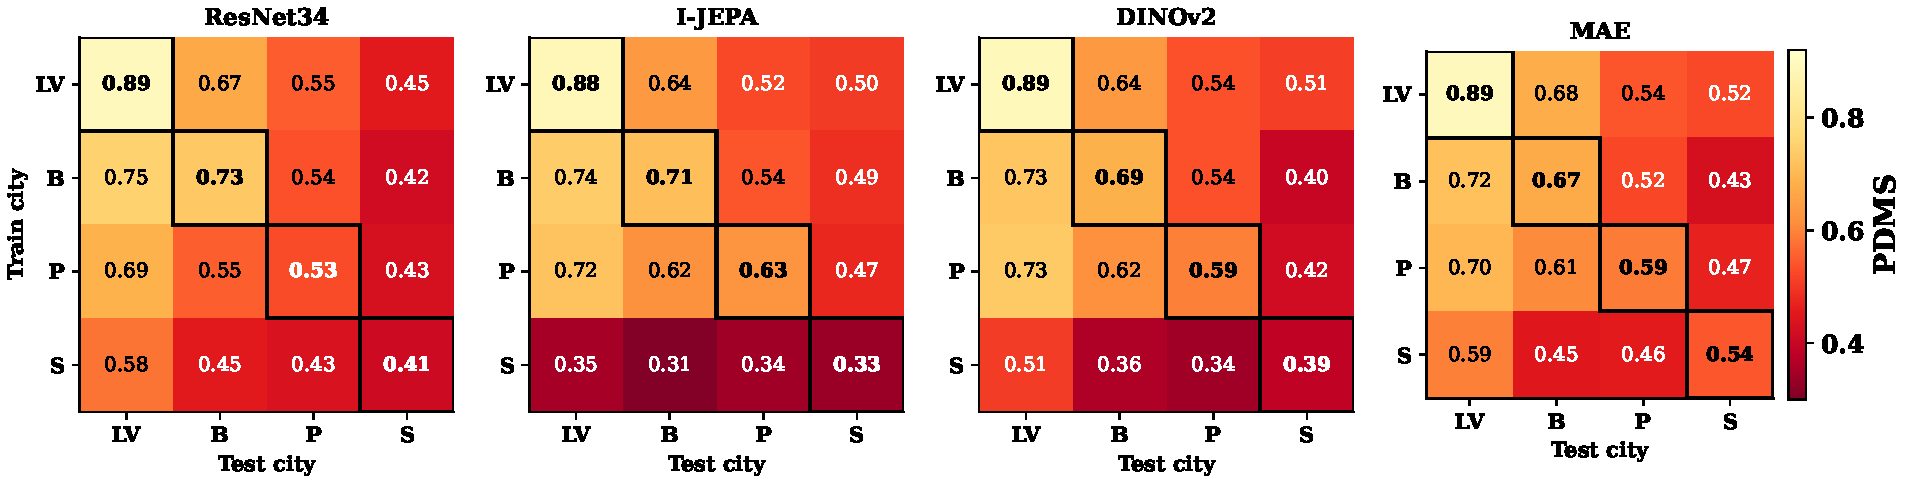
\includegraphics[width=0.48\textwidth]{iros/fig1_tf_pdms_heatmaps.pdf}
    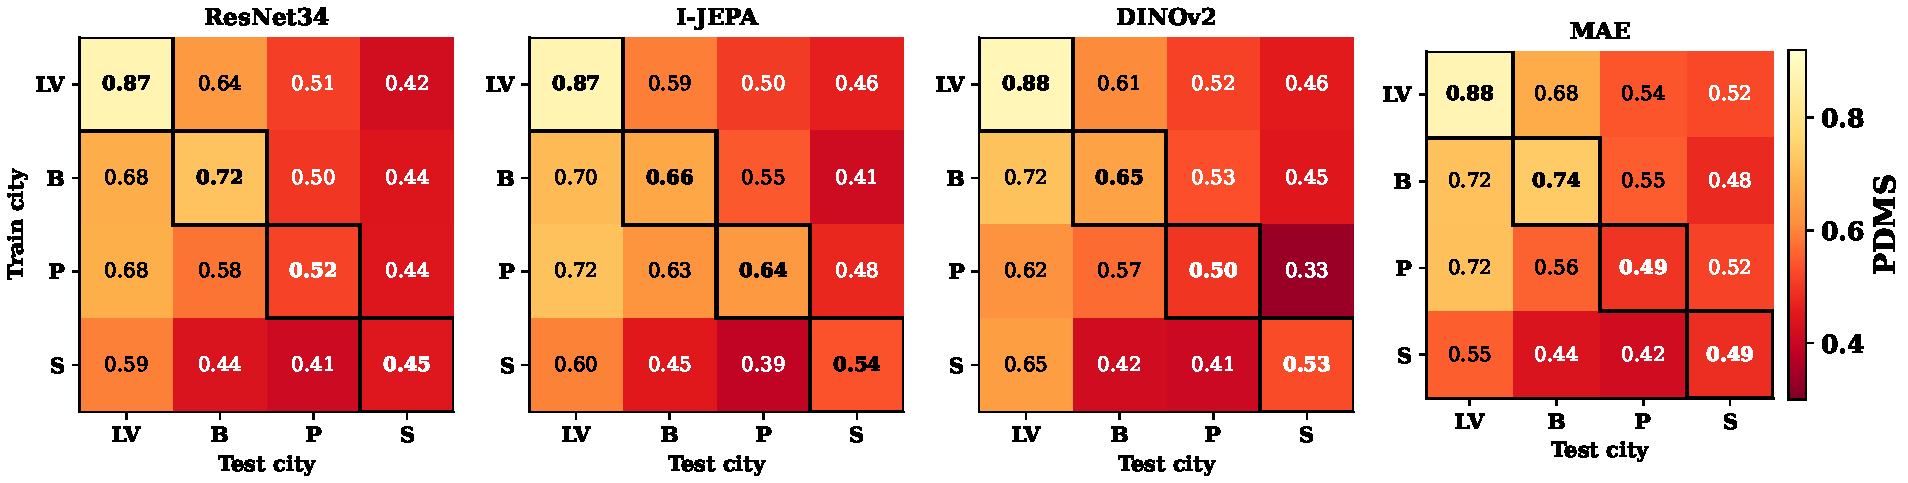
\includegraphics[width=0.48\textwidth]{iros/fig1_latf_pdms_heatmaps.pdf}
    \caption{Four-city cross-city PDMS matrices for TransFuser (left) and Latent TransFuser (right), pulled directly from our earlier cross-city benchmark study~\cite{naeinian-cross-city-2026}. Rows are training cities, columns are test cities, and each panel is a backbone family. The diagonal is in-distribution; off-diagonal cells expose the representation-dependent generalization gap. For every backbone, the Singapore column is the harshest; for supervised ResNet-34 (top-left panel), the off-diagonal penalty is larger and more uneven than for the frozen SSL panels.}
    \label{fig:iros-pdms-heatmaps}
\end{figure}

\subsection{OOD PDMS Analysis}
\label{sec:exp-phase1-ood}

The most direct open-loop evidence comes from transfer from Boston to Singapore on nuScenes. The supervised Swin backbone inflates from 0.60 to 5.86 average L2 and from 0.32 to 6.19 average collision rate, corresponding to 9.77$\times$ and 19.34$\times$ degradation. Replacing the backbone with a domain-specific SSL representation changes the picture entirely: the rectangular, frozen nuScenes-pretrained I-JEPA ViT-S/14 model yields an error ratio of only 1.20$\times$ in L2 and 0.75$\times$ in collision rate for the same transfer~\cite{naeinian-cross-city-2026}. The planning architecture is unchanged, so the improved robustness must come from the representation.

The closed-loop NAVSIM results point in the same direction. Generic large-scale SSL often matches or slightly exceeds the supervised ResNet34 baseline under single-city transfer, and domain-specific SSL is more reliable still. In the LiDAR-free Latent TransFuser setting, nuScenes-pretrained MAE improves average OOD PDMS by more than four points for Boston-, Pittsburgh-, and Las Vegas-trained models and by roughly three points for Singapore-trained models~\cite{naeinian-cross-city-2026}. The effect is therefore not a quirk of one backbone family or one planner: once city shift is explicit, self-supervised initialization systematically narrows the gap between in-domain and out-of-domain behavior.

\begin{figure}[ht]
    \centering
    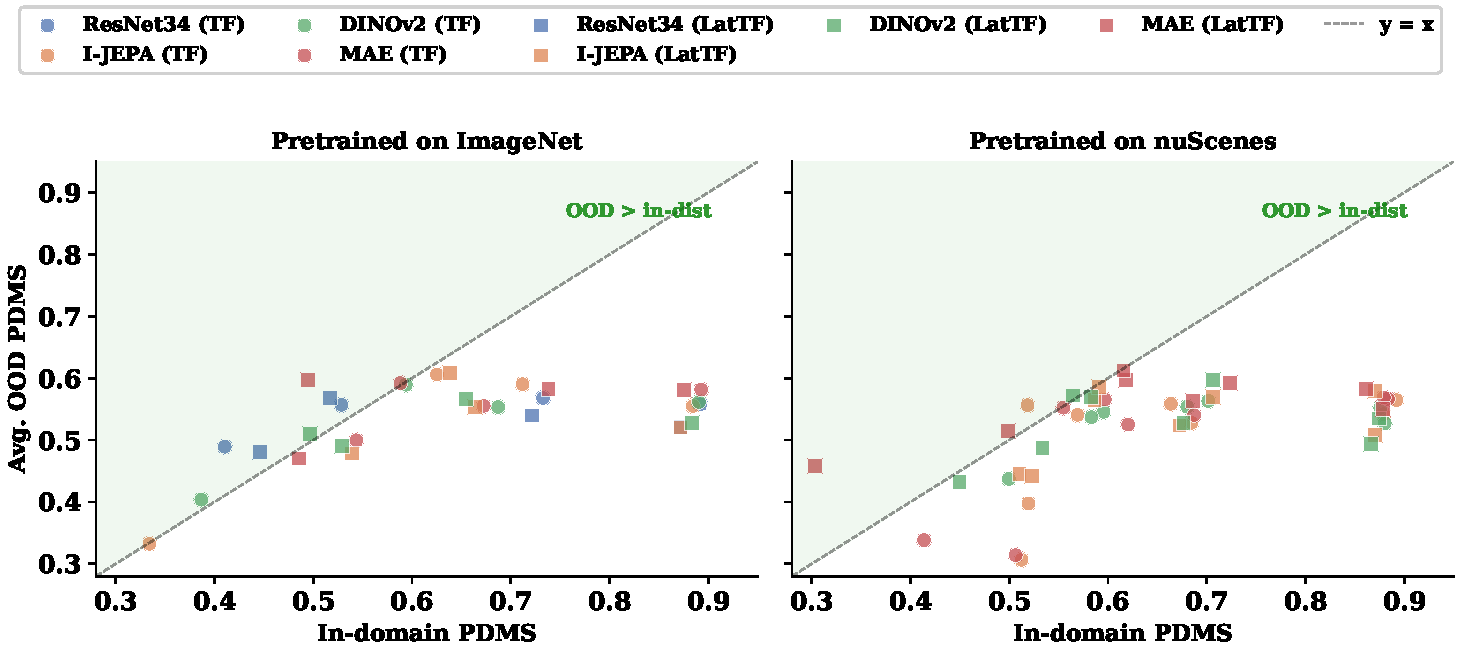
\includegraphics[width=0.75\textwidth]{iros/fig3_indomain_vs_ood.pdf}
    \caption{In-distribution PDMS versus average out-of-distribution PDMS across every cross-city configuration. Each point is one trained model; the diagonal is the reference ``no transfer penalty'' line. Points above the diagonal indicate in-distribution overfitting relative to OOD behavior. Supervised backbones (red) cluster further from the diagonal than frozen SSL backbones (blue) at every in-distribution score, consistent with the representation hypothesis. Source: Fig.~3 of our earlier cross-city benchmark study~\cite{naeinian-cross-city-2026}.}
    \label{fig:iros-indomain-vs-ood}
\end{figure}

Closed-loop cross-city transfer is further evaluated using the NAVSIM benchmark with the Performance Degradation Metric Score (PDMS), which measures driving task completion while penalizing infractions (higher is better). Table~\ref{tab:navsim_pdms_merged} reports PDMS across four cities --- Las Vegas (LV), Boston (B), Pittsburgh (P), and Singapore (S) --- for both TransFuser and Latent TransFuser under the NAVSIM v2.2 devkit; Table~\ref{tab:navsim_pdms_merged_v11} is the same matrix re-evaluated with the official NAVSIM v1.1 devkit as a defensive check against devkit-version confounders. For each backbone, we report results from all-city and single-city training to illustrate the impact of the geographic domain shift on closed-loop performance.

% Full NAVSIM v2.2 cross-city PDMS matrix (legacy devkit).
% Retained as provenance for the companion paper's numbers; the canonical
% thesis matrix is the v1.1 table (tab_navsim_pdms_merged_v11.tex).
\begin{sidewaystable}[p]
    \centering
    \caption[NAVSIM v2.2 cross-city PDMS matrix (legacy).]{%
    Full closed-loop cross-city PDMS matrix on NAVSIM, devkit v2.2 (legacy).
    Each row is a single trained model. The left block (\emph{Train City}) marks which of the four cities were used for training; \cmark indicates inclusion. Total combines performance across all four evaluation cities for each planner. All numbers are PDMS (\%); higher is better.
    How to read it: rows with four training cities are the all-city baselines, and their \emph{Total} column is mixed-city interpolation performance. Rows with a single training city are zero-shot transfer probes; non-checked columns under each planner are the out-of-distribution cells, and the gap between the in-distribution column and the three OOD columns quantifies the geographic transfer penalty. This matrix is retained for direct comparison with the companion cross-city benchmark paper~\cite{naeinian-cross-city-2026}; the thesis claims use the v1.1 re-evaluation in~\reftab{tab:navsim_pdms_merged_v11}.}
    \label{tab:navsim_pdms_merged}
    \scriptsize
    \setlength{\tabcolsep}{2pt}
    \renewcommand{\arraystretch}{0.95}
    \resizebox{\textwidth}{!}{%
    \begin{tabular}{|l|cccc|ccccc|ccccc|}
    \toprule
    \multirow{2}{*}{\textbf{Backbone}}
    & \multicolumn{4}{c|}{\textbf{Train City}}
    & \multicolumn{5}{c|}{\textbf{TransFuser (PDMS \%)}}
    & \multicolumn{5}{c|}{\textbf{Latent TransFuser (PDMS \%)}} \\
    \cmidrule(lr){2-5}\cmidrule(lr){6-10}\cmidrule(lr){11-15}
    & LV & B & P & S
    & LV & B & P & S & Total
    & LV & B & P & S & Total \\
    \midrule
    ResNet-34 supervised          & \cmark & \cmark & \cmark & \cmark & 88.4 & \textbf{81.4} & \textbf{75.7} & \textbf{59.9} & \textbf{79.2} & 87.0 & \textbf{79.3} & \textbf{74.4} & \textbf{67.2} & \textbf{79.0} \\
    ResNet-34 supervised          & --     & \cmark & --     & --     & 75.3 & 73.3 & 53.6 & 41.5 & 65.0 & 67.9 & 72.2 & 50.0 & 44.0 & 61.8 \\
    ResNet-34 supervised          & \cmark & --     & --     & --     & \textbf{89.2} & 67.0 & 55.1 & 45.3 & 68.6 & \textbf{87.2} & 63.6 & 50.9 & 41.9 & 65.5 \\
    ResNet-34 supervised          & --     & --     & \cmark & --     & 68.8 & 55.3 & 52.9 & 43.0 & 57.4 & 68.2 & 58.0 & 51.7 & 44.3 & 58.0 \\
    ResNet-34 supervised          & --     & --     & --     & \cmark & 57.9 & 45.5 & 43.4 & 41.0 & 48.5 & 59.3 & 43.9 & 41.1 & 44.6 & 48.6 \\
    \midrule
    I-JEPA ViT-H/14 frozen        & \cmark & \cmark & \cmark & \cmark & 86.5 & 77.1 & 71.2 & 68.1 & 77.6 & 85.0 & 76.5 & 69.6 & 68.7 & 76.7 \\
    I-JEPA ViT-H/14 100\% trainable & \cmark & \cmark & \cmark & \cmark & 87.4 & \textbf{77.7} & 68.8 & 64.2 & 77.0 & \textbf{89.3} & \textbf{77.8} & \textbf{73.0} & 67.6 & \textbf{79.1} \\
    I-JEPA ViT-S/14 nuSc rect., frozen        & \cmark & \cmark & \cmark & \cmark & 88.4 & 77.5 & \textbf{71.5} & 68.4 & \textbf{78.5} & 87.6 & 76.5 & 71.1 & 57.0 & 76.1 \\
    I-JEPA ViT-S/14 nuSc rect., trainable     & \cmark & \cmark & \cmark & \cmark & 88.9 & \textbf{77.7} & 70.8 & 67.0 & 78.4 & 86.6 & 74.8 & 67.2 & 65.3 & 75.7 \\
    I-JEPA ViT-S/14 nuSc sq., frozen          & \cmark & \cmark & \cmark & \cmark & 85.5 & 75.9 & 68.2 & \textbf{69.4} & 76.6 & 84.5 & 73.3 & 68.0 & 65.1 & 74.7 \\
    I-JEPA ViT-S/14 nuSc sq., trainable       & \cmark & \cmark & \cmark & \cmark & 86.7 & 76.2 & 70.9 & 65.7 & 77.0 & 82.9 & 69.8 & 59.1 & \textbf{70.2} & 72.1 \\
    I-JEPA ViT-H/14 frozen        & --     & \cmark & --     & --     & 74.1 & 71.2 & 54.2 & 48.8 & 65.2 & 70.2 & 66.4 & 54.7 & 41.2 & 61.3 \\
    I-JEPA ViT-H/14 trainable     & --     & \cmark & --     & --     & 72.5 & 68.0 & 52.4 & 40.9 & 62.1 & 71.7 & 68.5 & 55.0 & 47.8 & 63.6 \\
    I-JEPA ViT-H/14 frozen        & \cmark & --     & --     & --     & 88.4 & 63.6 & 52.5 & 50.5 & 67.6 & 87.2 & 59.2 & 50.5 & 46.4 & 64.8 \\
    I-JEPA ViT-H/14 trainable     & \cmark & --     & --     & --     & 88.3 & 62.2 & 52.9 & 50.1 & 67.1 & 83.1 & 62.0 & 52.5 & 44.7 & 64.4 \\
    I-JEPA ViT-H/14 frozen        & --     & --     & \cmark & --     & 72.1 & 62.2 & 62.5 & 47.4 & 63.3 & 72.0 & 62.9 & 63.9 & 47.5 & 63.7 \\
    I-JEPA ViT-H/14 trainable     & --     & --     & \cmark & --     & 70.1 & 60.4 & 60.1 & 37.4 & 60.0 & 64.0 & 60.1 & 55.8 & 33.8 & 56.4 \\
    I-JEPA ViT-H/14 frozen        & --     & --     & --     & \cmark & 35.1 & 30.5 & 34.1 & 33.4 & 33.2 & 59.6 & 45.1 & 38.8 & 53.9 & 50.1 \\
    I-JEPA ViT-H/14 trainable     & --     & --     & --     & \cmark & 58.1 & 44.9 & 43.8 & 48.8 & 49.7 & 64.0 & 44.9 & 41.3 & 50.8 & 51.5 \\
    \midrule
    DINOv2 ViT-S/14 frozen                    & \cmark & \cmark & \cmark & \cmark & 88.7 & 78.4 & 70.2 & 66.1 & 78.3 & 87.6 & 76.5 & 69.8 & 62.2 & 76.6 \\
    DINOv2 ViT-S/14 trainable                 & \cmark & \cmark & \cmark & \cmark & 86.0 & 74.4 & 66.0 & 68.9 & 75.7 & 86.4 & 72.1 & 63.2 & 56.0 & 72.5 \\
    DINOv2 ViT-S/14 nuSc rect., frozen        & \cmark & \cmark & \cmark & \cmark & 87.2 & 78.1 & 72.1 & 71.0 & 78.8 & 87.9 & 75.5 & 70.2 & 66.6 & 77.2 \\
    DINOv2 ViT-S/14 nuSc rect., trainable     & \cmark & \cmark & \cmark & \cmark & 88.5 & 79.7 & 74.1 & 67.9 & \textbf{79.7} & \textbf{88.3} & \textbf{79.8} & \textbf{73.1} & \textbf{71.3} & \textbf{79.9} \\
    DINOv2 ViT-S/14 nuSc sq., frozen          & \cmark & \cmark & \cmark & \cmark & 88.0 & \textbf{80.4} & \textbf{75.9} & 65.8 & \textbf{79.7} & 86.8 & 75.0 & 69.5 & 61.2 & 75.7 \\
    DINOv2 ViT-S/14 nuSc sq., trainable       & \cmark & \cmark & \cmark & \cmark & 87.7 & 77.1 & 68.4 & \textbf{71.5} & 78.0 & 83.7 & 73.0 & 64.2 & 66.7 & 73.8 \\
    \midrule
    MAE ViT-B/16 frozen                       & \cmark & \cmark & \cmark & \cmark & 89.5 & 80.9 & 75.1 & 65.5 & 80.2 & 87.6 & 76.9 & 70.5 & 69.5 & 78.0 \\
    MAE ViT-B/16 trainable                    & \cmark & \cmark & \cmark & \cmark & 86.3 & 78.6 & 69.3 & 67.8 & 77.6 & 86.3 & 76.5 & 68.5 & \textbf{74.9} & 77.9 \\
    MAE ViT-S/14 nuSc rect., frozen           & \cmark & \cmark & \cmark & \cmark & \textbf{90.3} & 80.2 & 74.2 & \textbf{73.7} & 81.4 & 85.3 & 77.3 & 72.9 & 69.9 & 77.9 \\
    MAE ViT-S/14 nuSc rect., trainable        & \cmark & \cmark & \cmark & \cmark & 89.9 & \textbf{82.4} & \textbf{77.4} & 72.6 & \textbf{82.4} & 89.2 & \textbf{79.9} & 70.2 & 68.9 & \textbf{79.3} \\
    MAE ViT-S/14 nuSc sq., frozen             & \cmark & \cmark & \cmark & \cmark & 88.9 & 78.6 & 73.7 & 68.3 & 79.4 & 84.5 & 75.2 & 71.5 & 67.3 & 76.3 \\
    MAE ViT-S/14 nuSc sq., trainable          & \cmark & \cmark & \cmark & \cmark & 87.4 & 77.8 & 74.2 & 70.6 & 79.2 & 85.8 & 77.7 & \textbf{74.4} & 64.1 & 77.6 \\
    \bottomrule
    \end{tabular}}%

    \vspace{0.6em}
    \footnotesize
    \emph{Single-city transfer rows for DINOv2 and MAE (Boston, Pittsburgh, Las~Vegas, Singapore) follow the same convention and are reported in the companion paper's supplementary material~\cite{naeinian-cross-city-2026}; the reduced set above is retained as the minimum provenance needed to justify the v1.1 re-evaluation used for all thesis claims.}
\end{sidewaystable}

% Full NAVSIM v1.1 cross-city PDMS matrix, canonical thesis table.
\begin{sidewaystable}[p]
    \centering
    \caption[NAVSIM v1.1 cross-city PDMS matrix (canonical).]{%
    Full closed-loop cross-city PDMS matrix on NAVSIM, devkit v1.1. This is the canonical closed-loop table used for every cross-city claim in the thesis. Each row is a single trained model; \emph{Train City} marks the cities used to fit that model. The two planner blocks (\emph{TransFuser}, \emph{Latent TransFuser}) report destination-city PDMS on the four NAVSIM test splits (LV, B, P, S) plus a \emph{Total} column averaging the four.
    How to read it: rows with all four training cities checked measure mixed-city interpolation; rows with a single training city measure zero-shot geographic transfer, in which case the three non-checked columns are the out-of-distribution cells. The gap between the in-distribution column and the OOD mean under a single planner isolates the transfer penalty; comparing the same row across the two planners separates backbone effects from head effects. All values are PDMS percentages; higher is better.}
    \label{tab:navsim_pdms_merged_v11}
    \scriptsize
    \setlength{\tabcolsep}{2pt}
    \renewcommand{\arraystretch}{0.95}
    \resizebox{\textwidth}{!}{%
    \begin{tabular}{|l|cccc|ccccc|ccccc|}
    \toprule
    \multirow{2}{*}{\textbf{Backbone}}
    & \multicolumn{4}{c|}{\textbf{Train City}}
    & \multicolumn{5}{c|}{\textbf{TransFuser (PDMS \%)}}
    & \multicolumn{5}{c|}{\textbf{Latent TransFuser (PDMS \%)}} \\
    \cmidrule(lr){2-5}\cmidrule(lr){6-10}\cmidrule(lr){11-15}
    & LV & B & P & S
    & LV & B & P & S & Total
    & LV & B & P & S & Total \\
    \midrule
    ResNet-34 supervised          & \cmark & \cmark & \cmark & \cmark & 86.6 & \textbf{78.4} & \textbf{73.8} & \textbf{64.0} & \textbf{77.9} & \textbf{89.0} & \textbf{82.5} & \textbf{80.3} & \textbf{66.5} & \textbf{81.7} \\
    ResNet-34 supervised          & --     & \cmark & --     & --     & 75.3 & 73.3 & 53.6 & 41.5 & 65.0 & 67.3 & 71.7 & 54.5 & 45.0 & 62.6 \\
    ResNet-34 supervised          & \cmark & --     & --     & --     & \textbf{89.2} & 67.0 & 55.1 & 45.3 & 68.6 & 86.9 & 62.1 & 53.2 & 42.3 & 65.5 \\
    ResNet-34 supervised          & --     & --     & \cmark & --     & 68.8 & 55.3 & 52.9 & 43.0 & 57.4 & 67.7 & 57.5 & 53.0 & 46.5 & 58.3 \\
    ResNet-34 supervised          & --     & --     & --     & \cmark & 56.6 & 45.4 & 49.6 & 42.1 & 49.5 & 57.4 & 42.6 & 45.1 & 45.5 & 48.5 \\
    \midrule
    I-JEPA ViT-H/14 frozen        & \cmark & \cmark & \cmark & \cmark & 85.3 & 75.7 & 72.4 & 67.3 & 76.9 & 83.7 & 75.2 & 70.9 & \textbf{68.3} & 76.1 \\
    I-JEPA ViT-H/14 trainable     & \cmark & \cmark & \cmark & \cmark & 86.6 & \textbf{77.1} & 70.6 & 64.8 & 77.0 & \textbf{88.7} & \textbf{77.3} & 75.1 & 67.1 & \textbf{79.1} \\
    I-JEPA ViT-S/14 nuSc rect., frozen        & \cmark & \cmark & \cmark & \cmark & 87.3 & 77.0 & \textbf{74.3} & \textbf{69.2} & \textbf{78.7} & 86.6 & 73.3 & 69.7 & 59.9 & 74.9 \\
    I-JEPA ViT-S/14 nuSc rect., trainable     & \cmark & \cmark & \cmark & \cmark & 89.0 & 76.8 & 73.3 & 67.0 & 78.6 & 86.2 & 73.9 & 74.7 & 59.5 & 75.9 \\
    I-JEPA ViT-S/14 nuSc sq., frozen          & \cmark & \cmark & \cmark & \cmark & 84.8 & 75.1 & 69.7 & 69.1 & 76.3 & 83.8 & 73.2 & 68.6 & 61.5 & 74.0 \\
    I-JEPA ViT-S/14 nuSc sq., trainable       & \cmark & \cmark & \cmark & \cmark & 85.8 & 75.7 & 73.0 & 65.2 & 76.9 & 87.3 & 76.4 & \textbf{75.3} & 67.7 & 78.5 \\
    I-JEPA ViT-H/14 frozen        & --     & \cmark & --     & --     & 72.5 & 69.9 & 58.2 & 50.1 & 65.3 & 69.4 & 67.5 & 62.2 & 42.2 & 63.1 \\
    I-JEPA ViT-H/14 trainable     & --     & \cmark & --     & --     & 72.0 & 68.9 & 60.1 & 42.0 & 63.9 & 70.7 & 68.2 & 60.7 & 48.7 & 64.5 \\
    I-JEPA ViT-H/14 frozen        & \cmark & --     & --     & --     & 86.9 & 61.2 & 53.7 & 51.4 & 66.7 & 85.9 & 57.5 & 51.9 & 47.8 & 64.3 \\
    I-JEPA ViT-H/14 trainable     & \cmark & --     & --     & --     & 87.7 & 60.1 & 53.9 & 51.3 & 66.7 & 82.7 & 60.3 & 54.8 & 44.3 & 64.2 \\
    I-JEPA ViT-H/14 frozen        & --     & --     & \cmark & --     & 71.4 & 61.3 & 64.5 & 49.5 & 63.5 & 71.8 & 63.5 & 69.0 & 48.6 & 65.0 \\
    I-JEPA ViT-H/14 trainable     & --     & --     & \cmark & --     & 69.1 & 59.6 & 65.3 & 39.0 & 60.7 & 63.7 & 60.1 & 59.4 & 35.4 & 57.3 \\
    I-JEPA ViT-H/14 frozen        & --     & --     & --     & \cmark & 36.0 & 35.9 & 45.1 & 35.6 & 37.7 & 58.3 & 44.6 & 43.0 & 55.6 & 50.6 \\
    I-JEPA ViT-H/14 trainable     & --     & --     & --     & \cmark & 56.7 & 45.3 & 48.0 & 50.3 & 50.4 & 62.7 & 43.9 & 44.4 & 52.8 & 51.7 \\
    \midrule
    DINOv2 ViT-S/14 frozen                    & \cmark & \cmark & \cmark & \cmark & 87.7 & 77.0 & 71.5 & 66.0 & 77.7 & 86.4 & 72.8 & 67.2 & 59.2 & 74.1 \\
    DINOv2 ViT-S/14 trainable                 & \cmark & \cmark & \cmark & \cmark & 85.4 & 73.5 & 67.6 & 68.9 & 75.6 & 82.7 & 68.9 & 64.0 & 54.2 & 70.2 \\
    DINOv2 ViT-S/14 nuSc rect., frozen        & \cmark & \cmark & \cmark & \cmark & 86.6 & 77.2 & 74.0 & 70.5 & 78.7 & 87.1 & 74.8 & 71.6 & \textbf{71.5} & 77.7 \\
    DINOv2 ViT-S/14 nuSc rect., trainable     & \cmark & \cmark & \cmark & \cmark & 87.9 & 79.0 & 76.2 & 67.4 & \textbf{79.6} & 87.3 & \textbf{78.5} & \textbf{75.7} & 66.7 & \textbf{79.0} \\
    DINOv2 ViT-S/14 nuSc sq., frozen          & \cmark & \cmark & \cmark & \cmark & 87.2 & \textbf{79.2} & \textbf{77.8} & 65.5 & 79.4 & 86.3 & 73.1 & 72.7 & 60.8 & 75.5 \\
    DINOv2 ViT-S/14 nuSc sq., trainable       & \cmark & \cmark & \cmark & \cmark & 86.3 & 75.9 & 69.0 & \textbf{71.2} & 77.3 & 86.7 & 73.6 & 70.6 & 71.2 & 77.0 \\
    \midrule
    MAE ViT-B/16 frozen                       & \cmark & \cmark & \cmark & \cmark & 89.0 & 80.8 & \textbf{78.7} & 65.1 & 80.7 & 81.7 & 70.7 & 62.8 & 69.9 & 72.7 \\
    MAE ViT-B/16 trainable                    & \cmark & \cmark & \cmark & \cmark & 85.4 & 78.0 & 73.9 & 67.4 & 78.0 & 88.7 & \textbf{81.9} & \textbf{80.0} & 61.6 & 80.6 \\
    MAE ViT-S/14 nuSc rect., frozen           & \cmark & \cmark & \cmark & \cmark & 89.2 & 79.1 & 75.1 & \textbf{73.1} & 80.7 & 87.4 & 79.2 & 79.8 & 64.6 & 79.8 \\
    MAE ViT-S/14 nuSc rect., trainable        & \cmark & \cmark & \cmark & \cmark & 89.3 & \textbf{81.2} & 78.4 & 72.1 & \textbf{81.9} & 86.2 & 79.7 & 77.8 & 72.3 & 80.3 \\
    MAE ViT-S/14 nuSc sq., frozen             & \cmark & \cmark & \cmark & \cmark & 87.7 & 77.3 & 75.2 & 67.8 & 78.9 & 86.4 & 75.0 & 70.3 & 67.9 & 76.7 \\
    MAE ViT-S/14 nuSc sq., trainable          & \cmark & \cmark & \cmark & \cmark & 86.9 & 77.3 & 76.3 & 70.3 & 79.2 & \textbf{89.3} & 78.5 & 78.0 & \textbf{74.1} & \textbf{81.4} \\
    MAE ViT-B/16 frozen                       & --     & \cmark & --     & --     & 70.6 & 67.0 & 56.8 & 43.4 & 62.4 & 71.8 & 73.4 & 60.0 & 48.7 & 66.3 \\
    MAE ViT-B/16 trainable                    & --     & \cmark & --     & --     & 70.6 & 67.3 & 58.0 & 41.9 & 62.5 & 69.4 & 73.1 & 61.3 & 53.7 & 66.5 \\
    MAE ViT-B/16 frozen                       & \cmark & --     & --     & --     & 88.3 & 66.2 & 55.2 & 52.9 & 69.3 & 86.6 & 66.0 & 56.1 & 52.2 & 68.8 \\
    MAE ViT-B/16 trainable                    & \cmark & --     & --     & --     & 87.4 & 59.8 & 53.2 & 51.6 & 66.4 & 87.8 & 63.3 & 56.0 & 51.0 & 68.1 \\
    MAE ViT-B/16 frozen                       & --     & --     & \cmark & --     & 69.3 & 59.9 & 61.1 & 48.9 & 61.5 & 71.2 & 54.8 & 50.4 & 52.6 & 59.1 \\
    MAE ViT-B/16 trainable                    & --     & --     & \cmark & --     & 73.0 & 65.6 & 68.8 & 40.8 & 64.8 & 64.4 & 63.9 & 61.0 & 35.7 & 59.1 \\
    MAE ViT-B/16 frozen                       & --     & --     & --     & \cmark & 58.0 & 45.3 & 51.2 & 56.7 & 52.5 & 54.6 & 44.0 & 46.6 & 49.7 & 49.0 \\
    MAE ViT-B/16 trainable                    & --     & --     & --     & \cmark & 51.0 & 46.0 & 52.2 & 36.0 & 47.3 & 55.6 & 43.8 & 48.0 & 42.5 & 48.4 \\
    \bottomrule
    \end{tabular}}
\end{sidewaystable}

\begin{table}[ht]
\centering
\caption[Boston-only v1.1 Latent TransFuser cross-city summary.]{%
Compact summary of the canonical Boston-trained Latent TransFuser rows from the v1.1 matrix in~\reftab{tab:navsim_pdms_merged_v11}. These four rows are used as the matched supervised-vs-SSL comparison throughout the thesis: each model is trained on Boston only and evaluated on every NAVSIM city. LV/B/P/S are destination-city PDMS percentages; the in-distribution column (bold) is Boston; \emph{OOD mean} averages the three remaining cities and \emph{Drop} is the in-distribution-minus-OOD-mean gap in percentage points. A smaller drop indicates a more geographically robust representation under a fixed planner. The MAE row has the best absolute OOD mean; the DINOv2 row has the smallest drop; the ResNet-34 row has the largest drop and is the supervised reference.}
\label{tab:navsim_pdms_boston_v11}
\vspace{0.35em}
\small
\renewcommand{\arraystretch}{1.15}
\setlength{\tabcolsep}{5pt}
\begin{tabular}{@{}>{\raggedright\arraybackslash}p{3.6cm} c c c c c c@{}}
\toprule
\textbf{Backbone} & \textbf{LV (\%)} & \textbf{B (\%)} & \textbf{P (\%)} & \textbf{S (\%)} & \textbf{OOD mean (\%)} & \textbf{Drop (pp)} \\
\midrule
\rowcolor{gray!12}
ResNet-34 supervised & 67.3 & \textbf{71.7} & 54.5 & 45.0 & 55.6 & \textbf{16.1} \\
MAE ViT-B/16 frozen  & 71.8 & \textbf{73.4} & 60.0 & 48.7 & \textbf{60.2} & 13.2 \\
I-JEPA ViT-H/14 frozen & 69.4 & \textbf{67.5} & 62.2 & 42.2 & 57.9 & 9.6 \\
DINOv2 ViT-S/14 frozen & 70.7 & \textbf{63.6} & 55.8 & 45.5 & 57.3 & \textbf{6.3} \\
\bottomrule
\end{tabular}
\end{table}

\FloatBarrier

\subsection{Best Training Ground (RQ2)}
\label{sec:exp-phase1-best-training-city}

Which source city gives the most transferable planner? \reffig{fig:iros-best-training-city} aggregates this across all backbones and heads. Las Vegas and Boston alternate as the top two; Pittsburgh is consistently mid-tier; Singapore is the worst single-city training source in every configuration, for the reasons discussed in the data card (\refapp{app:city-data-card}). The same pattern appears more compactly in the radar plot (\reffig{fig:iros-radar}), which shows per-city in-distribution and OOD PDMS for each of the strongest backbones. The radar reveals a useful operational criterion: the best single-city training source is the one whose in-distribution contour most nearly matches its OOD contour, i.e.\ whose model maintains similar competence under transfer rather than simply being strongest on its own city.

\begin{figure}[ht]
    \centering
    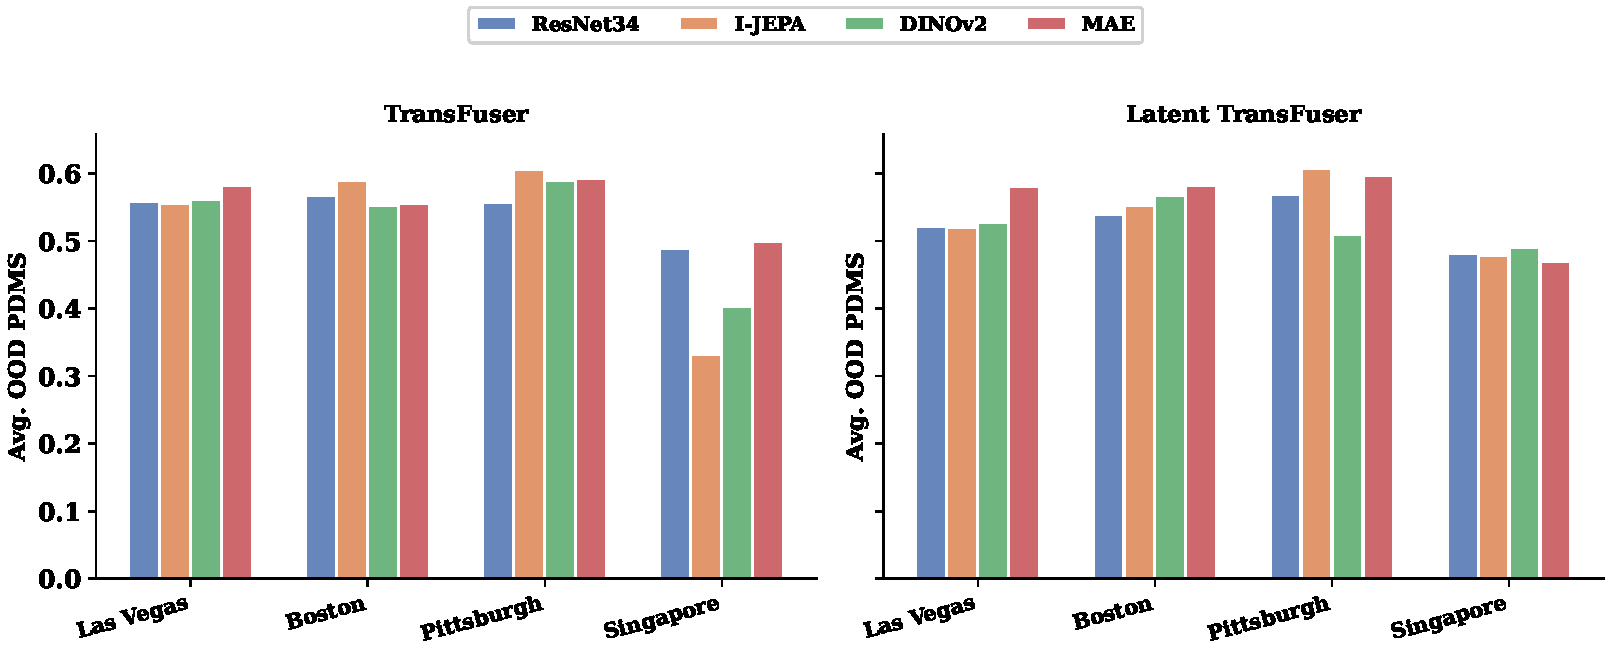
\includegraphics[width=0.75\textwidth]{iros/fig6_best_training_city.pdf}
    \caption{Average cross-city PDMS achieved by each of the four single-city training sources, grouped by backbone family. The ranking Las Vegas $\geq$ Boston $>$ Pittsburgh $>$ Singapore is stable across backbones; the absolute spread is larger for supervised ResNet-34 than for frozen SSL variants, consistent with the representation-centric account. Source: Fig.~6 of~\cite{naeinian-cross-city-2026}.}
    \label{fig:iros-best-training-city}
\end{figure}

\begin{figure}[ht]
    \centering
    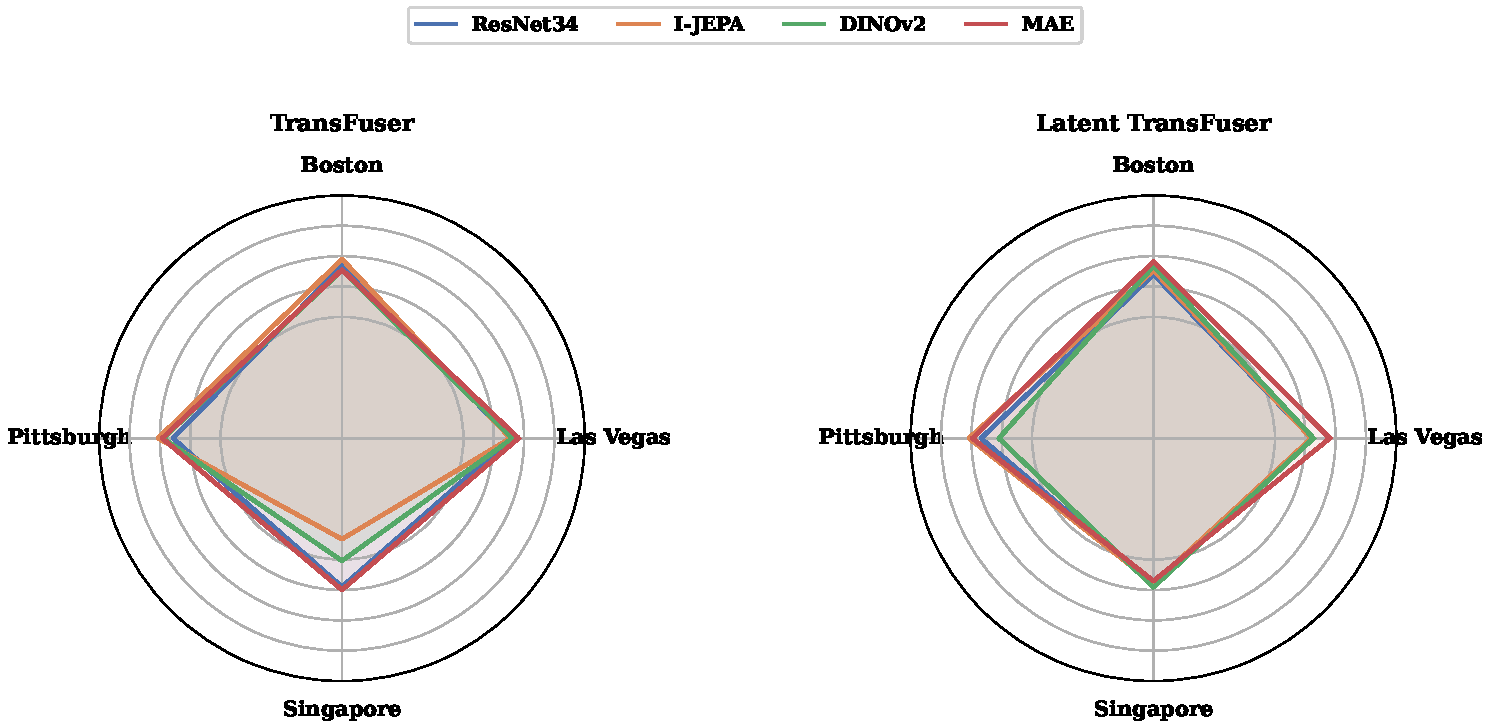
\includegraphics[width=0.9\textwidth]{iros/fig12_radar_summary.pdf}
    \caption{Radar summary of per-city PDMS by training source (rows) and backbone family (panels). The filled area is the average of the four per-city scores; wider, rounder areas correspond to more uniform transfer. Frozen SSL radars are more nearly circular than supervised ResNet radars, which is a compact visual restatement of the order-of-magnitude robustness claim. Source: Fig.~12 of~\cite{naeinian-cross-city-2026}.}
    \label{fig:iros-radar}
\end{figure}

\subsection{Transfer Asymmetry Analysis}
\label{sec:exp-phase1-asymmetry}

Transfer asymmetry is not noise; it is one of the most important findings of the benchmark. The hardest direction is typically from a right-hand-traffic city into Singapore, not the reverse. That asymmetry is consistent with a representational explanation: a backbone trained only on right-hand-traffic scenes can overfit to layout priors that become actively misleading in Singapore, whereas a model trained in Singapore is forced to encode some structure that remains useful when moved back to right-hand-traffic cities. Dataset scale compounds the effect. Singapore is also the smallest source domain in NAVSIM, so a model trained there has fewer opportunities to learn a diverse but reusable representation~\cite{naeinian-cross-city-2026}.

\begin{figure}[ht]
    \centering
    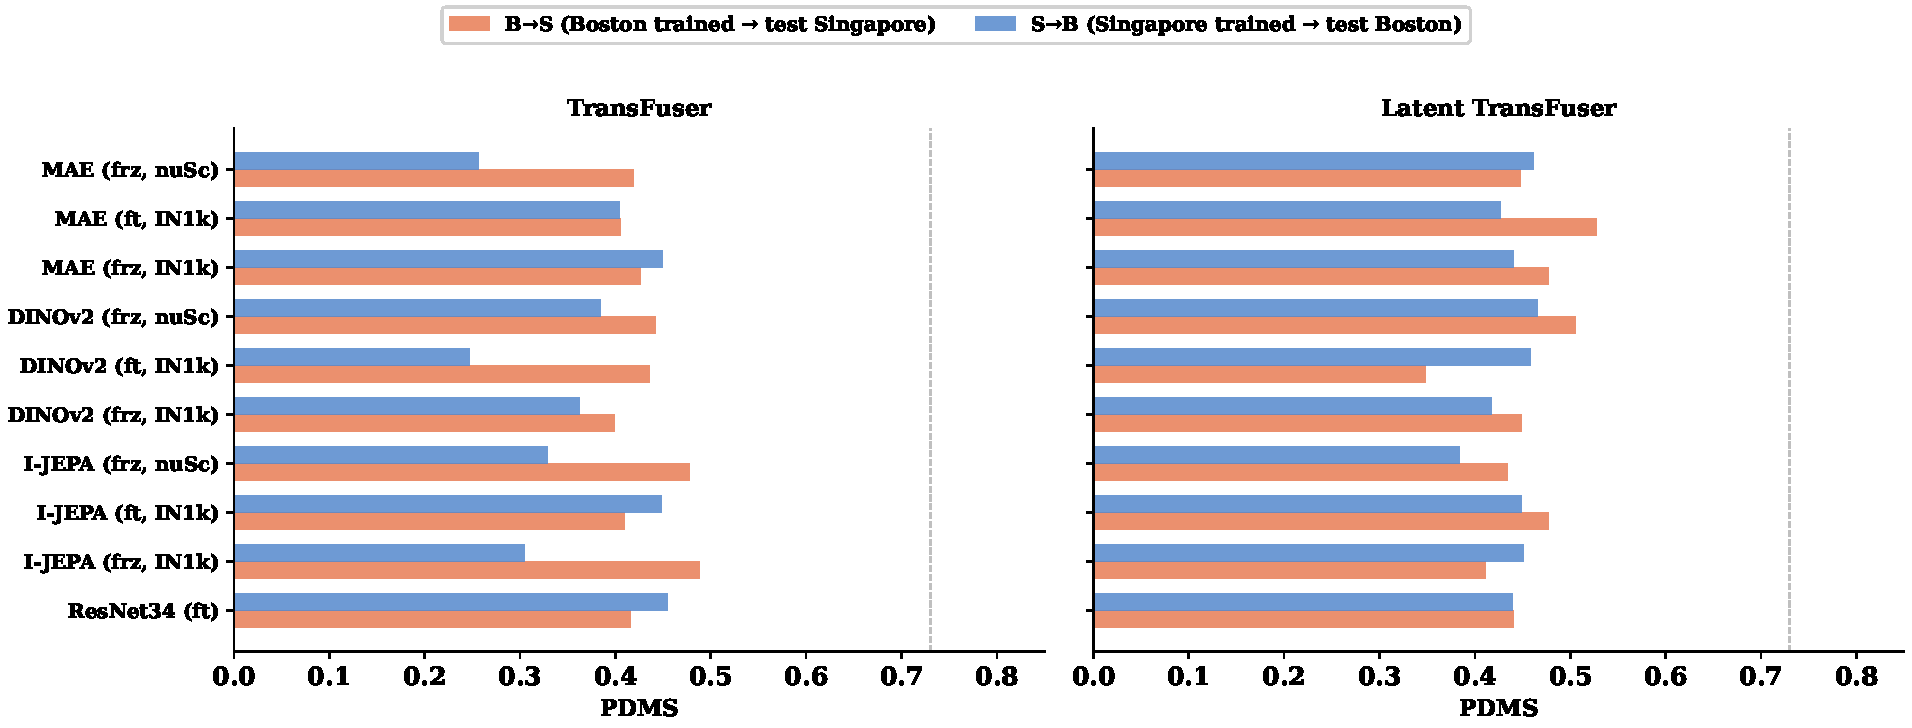
\includegraphics[width=0.7\textwidth]{iros/fig8_asymmetry.pdf}
    \caption[Boston--Singapore transfer asymmetry (bar chart).]{Boston$\leftrightarrow$Singapore transfer asymmetry. Bars are OOD PDMS at the destination; the grouped comparison isolates the direction of transfer. Boston$\rightarrow$Singapore is the harsher direction for every backbone, consistent with the dataset-scale and traffic-convention asymmetry discussed in-text. The absolute asymmetry gap is smaller for frozen SSL than for supervised ResNet-34. Source: Fig.~8 of~\cite{naeinian-cross-city-2026}.}
    \label{fig:iros-asymmetry}
\end{figure}

\subsection{Per-Metric Breakdown}
\label{sec:exp-phase1-metrics}

The phase-1 preprint primarily reports aggregate PDMS rather than a full decomposition into the five PDMS components for every transfer pair. For that reason, the thesis uses total PDMS as the main closed-loop robustness indicator in this chapter. The important point is that the gap is visible at the level of overall driving competence before any sub-score decomposition is introduced: geographic shift degrades planning quality substantially, and the degradation is consistently smaller when the backbone is self-supervised.

\begin{figure}[ht]
    \centering
    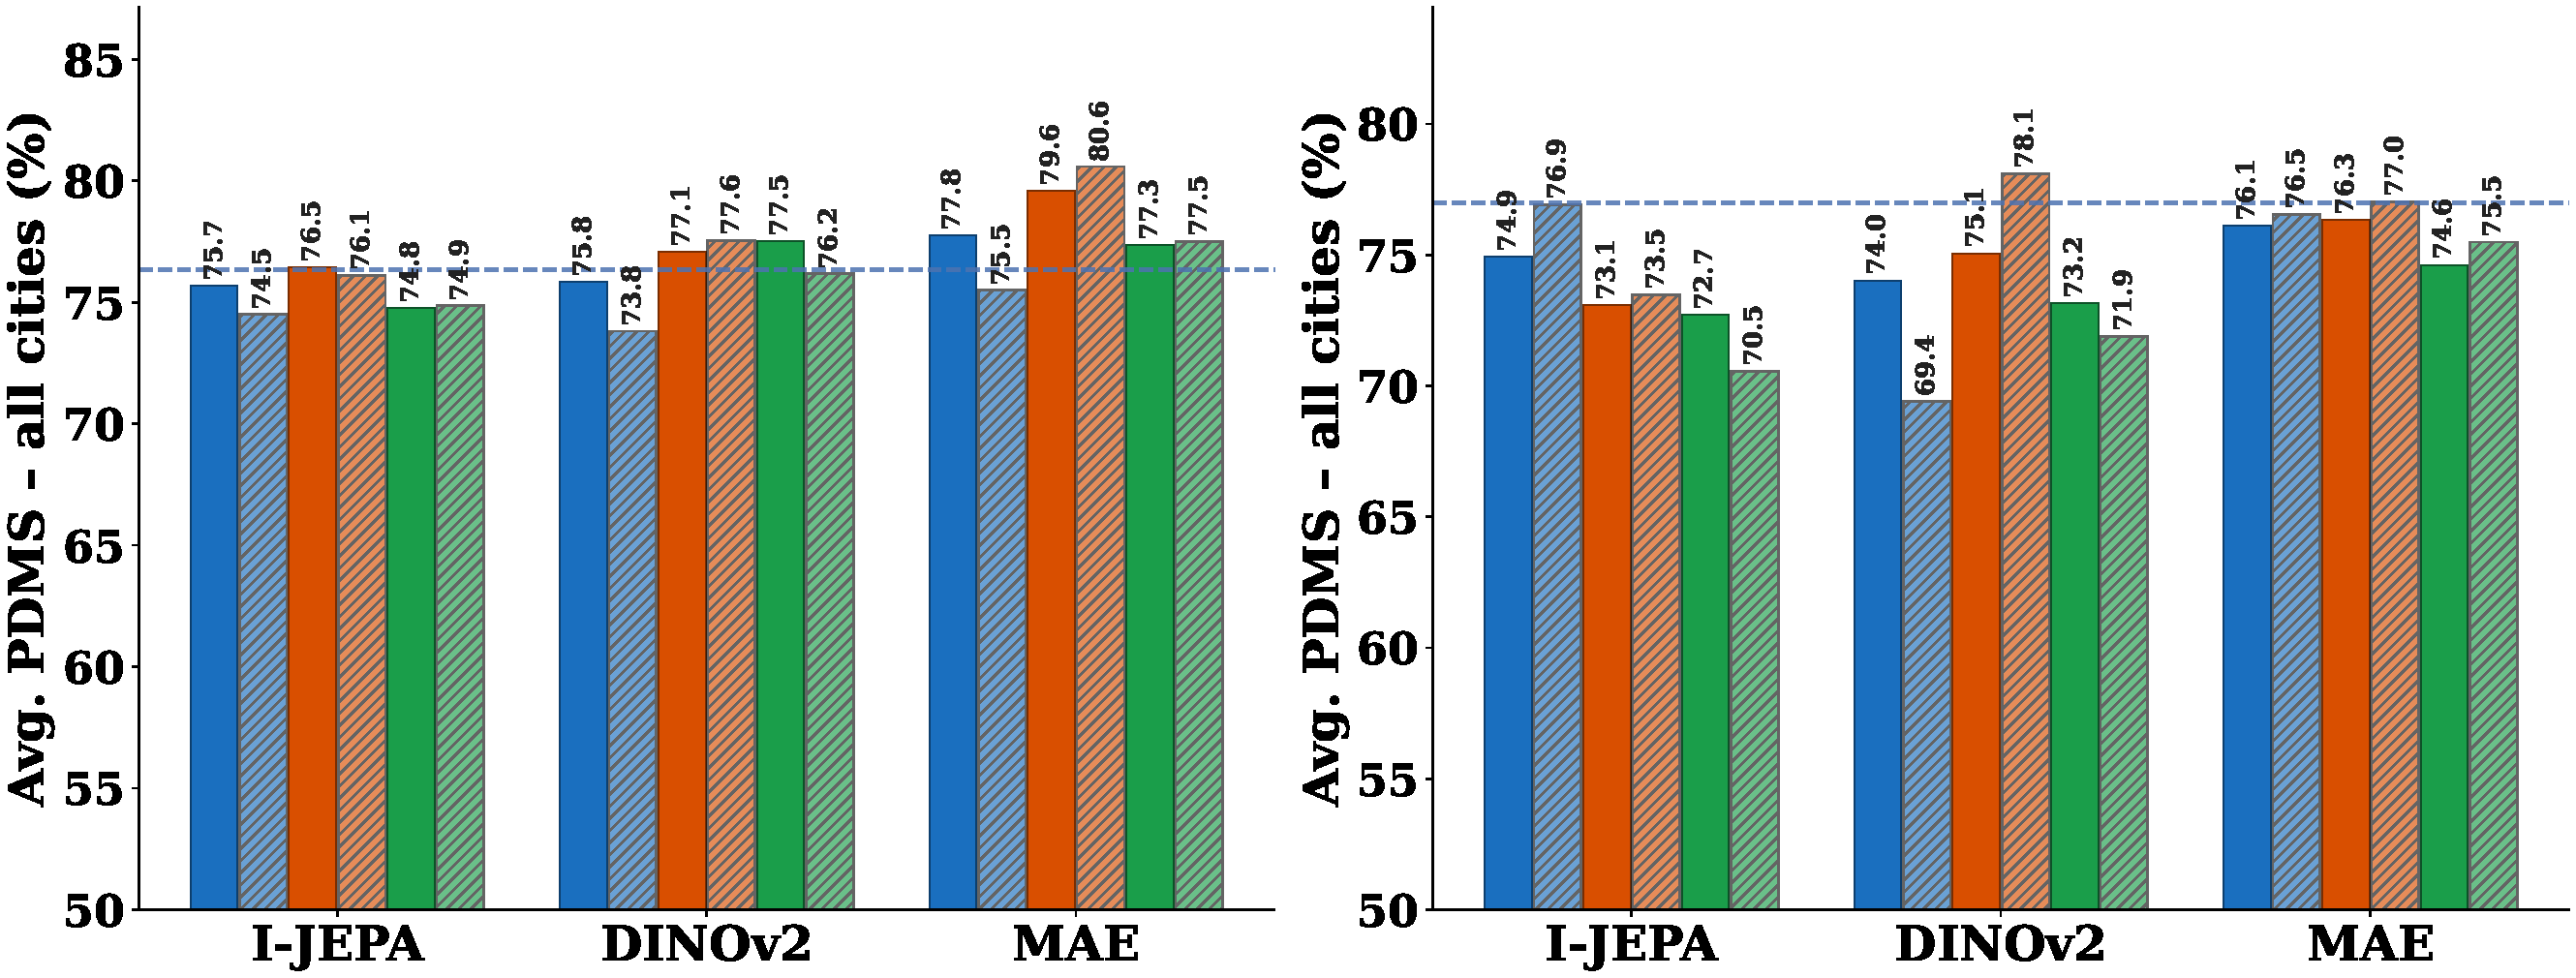
\includegraphics[width=0.85\textwidth]{iros/fig14_allcity_training.pdf}
    \caption{All-city training comparison. Mixed-city NAVSIM training pools examples from every city, which narrows the gap between supervised and SSL backbones as the dataset becomes geographically diverse. The takeaway is not that supervised backbones are equivalent to SSL --- they remain behind on the transfer matrices --- but that any benchmark that only reports mixed-city PDMS is measuring a regime in which the representation question is effectively washed out. Source: Fig.~14 of~\cite{naeinian-cross-city-2026}.}
    \label{fig:iros-allcity}
\end{figure}

% ============================================================================
\section{SSL Backbones in Generative Planning}
\label{sec:exp-phase2}

The generative-planning study revisits in-distribution NAVSIM under a planner that is designed to attenuate backbone contributions: DiffusionDrive~\cite{jia-diffusiondrive-2025}. Chapter~\ref{chap:methodology}, Section~\ref{sec:meth-dd-why} develops the rationale in full; the short form is that DiffusionDrive denoises trajectories from K-means anchor initializations in two steps, conditions through grid-sampled BEV cross-attention, and uses time-only FiLM, and the composite effect is a head that can produce good trajectories even when the image features are weak. This makes DiffusionDrive a deliberately hostile substrate for the representation claim. The goal of this study is therefore not to top an in-distribution leaderboard; it is to measure whether any backbone-dependent structure survives DiffusionDrive's attenuation, because that is the harder precondition for the cross-city generative study in \refsec{sec:exp-phase3}. The ViT adapter is held identical to the one used in the cross-city benchmark (both pipelines import \texttt{create\_image\_encoder} from the same TransFuser backbone module), so the planner head is the only manipulated variable between the two studies.

\begin{table}[ht]
\centering
\caption{DiffusionDrive + SSL backbone results on NAVSIM (all cities).}
\label{tab:diffusiondrive-allcity}
\begin{tabular}{lllcc}
\toprule
\textbf{Exp} & \textbf{Backbone} & \textbf{Modality} & \textbf{Frozen} & \textbf{PDMS} \\
\midrule
A12   & ResNet34              & C+L & ---       & 87.9 \\
A12-o & MAE (rect, trainable) & C+L & No        & 86.9 \\
A12-u & MAE (sq, trainable)   & C+L & No        & 86.8 \\
A12-q & I-JEPA (sq, trainable)& C+L & No        & 86.2 \\
A10-j & I-JEPA nuSc (rect, frozen) & C+L & Yes  & 85.2 \\
A10-p & I-JEPA nuSc (sq, frozen)   & C+L & Yes  & 86.3 \\
A13   & ResNet34 (camera-only)& C   & ---       & 86.6 \\
\bottomrule
\end{tabular}
\end{table}

\subsection{SSL vs.\ Supervised in Generative Planning}
\label{sec:exp-phase2-ssl-vs-sup}

The $\sim$1pp gap between SSL (86.2--86.9) and supervised ResNet34 (87.9) on all-city training mirrors the pattern from the cross-city benchmark. SSL features are slightly weaker in-distribution in this architecture as well. That observation is important in the context of the broader thesis: if mixed-city PDMS were the only question, stronger planner design could easily dominate the narrative. Instead, the small in-distribution cost becomes interesting only because later studies ask whether SSL repays that cost under domain shift.

\subsection{Camera-Only: SSL Partially Replaces LiDAR}
\label{sec:exp-phase2-camera-only}

The camera-only baseline is already stronger than one might expect. ResNet34 camera-only (A13) reaches 86.6 PDMS, only 1.3 points below the corresponding camera+LiDAR configuration at 87.9. This narrows the remaining question: the issue is no longer whether camera-only planning is viable at all, but whether stronger visual pretraining can close the residual gap without reintroducing expensive sensors. The planned I-JEPA camera-only experiment is therefore not a side experiment; it is the most direct test of whether SSL features can substitute for part of the geometric information usually supplied by LiDAR.

\paragraph{Planned I-JEPA camera-only comparison (designed, pending).}
Starting from the A13 ResNet-34 camera-only baseline ($86.6$ PDMS, \reftab{tab:diffusiondrive-allcity}), the supervised encoder is replaced with the strongest frozen SSL variant: I-JEPA ViT-S/14 nuScenes square, frozen (A10-p, $86.3$ PDMS in a camera+LiDAR configuration). Configuration is in \reftab{tab:exp-camonly-config}; pre-registered reading bands are in \reftab{tab:exp-camonly-bands}.

\begin{table}[ht]
\centering
\caption{Configuration for the planned I-JEPA camera-only comparison. All fields are held fixed to the A10-p / A13 hyperparameters; only the backbone and the LiDAR modality differ from their respective cells of \reftab{tab:diffusiondrive-allcity}.}
\label{tab:exp-camonly-config}
\small
\setlength{\tabcolsep}{6pt}
\renewcommand{\arraystretch}{1.15}
\begin{tabular}{@{}>{\raggedright\arraybackslash}p{3.6cm} >{\raggedright\arraybackslash}p{8.4cm}@{}}
\toprule
\textbf{Setting} & \textbf{Value} \\
\midrule
Backbone        & I-JEPA ViT-S/14, nuScenes square pre-training, frozen \\
Modality        & Camera only (LiDAR removed) \\
Optimizer       & Adam, constant LR $1\times10^{-4}$ \\
Epochs          & $20$ \\
Anchor bank     & $256$ K-means trajectories on \texttt{navtrain} \\
Denoising steps & $2$ (truncated) at inference \\
Training split  & \texttt{navtrain}, all cities \\
Reference rows  & A10-p ($86.3$ PDMS, C+L), A13 ($86.6$ PDMS, camera-only) \\
\bottomrule
\end{tabular}
\end{table}

\begin{table}[ht]
\centering
\caption{Pre-registered reading of the planned camera-only PDMS outcome. Bands are fixed before the run; interpretation follows directly.}
\label{tab:exp-camonly-bands}
\small
\setlength{\tabcolsep}{6pt}
\renewcommand{\arraystretch}{1.2}
\begin{tabular}{@{}>{\raggedright\arraybackslash}p{2.5cm} >{\raggedright\arraybackslash}p{2.9cm} >{\raggedright\arraybackslash}p{6.6cm}@{}}
\toprule
\textbf{Band} & \textbf{PDMS range} & \textbf{Interpretation} \\
\midrule
Full compensation & $\geq 86.6$            & Representation fully replaces LiDAR \\
Partial           & $85.5$--$86.5$         & Modest gain over supervised camera-only at no LiDAR cost \\
Null              & $< 85.0$               & Frozen SSL does not recover the LiDAR contribution at this scale \\
\bottomrule
\end{tabular}
\end{table}

\subsection{Frozen vs.\ Fine-Tuned Backbone}
\label{sec:exp-phase2-frozen}

Within DiffusionDrive, the I-JEPA results show that preprocessing matters at least as much as fine-tuning. The rectangular frozen run reaches 85.2 PDMS, the square-crop frozen run reaches 86.3, and the trainable square-crop run reaches 86.2. The simplest interpretation is that matching the pretraining geometry of the ViT is more important than unfreezing the backbone, at least on the mixed-city split. This fits the broader thesis argument that frozen SSL weights act as a form of implicit regularization: they preserve the pretrained invariances while still allowing the adapter and planner to specialize downstream.

% ============================================================================
\section{Cross-City Generative Planning Protocol (Designed; Pending)}
\label{sec:exp-phase3}

The cross-city generative study extends the representation-centric cross-city benchmark into the generative-planning regime. The protocol is already defined and the training pipeline is ready to launch; the experimental runs themselves are scheduled outside the window of this thesis and will be reported in a follow-up publication. We document the protocol here with the same level of detail as the completed studies so that the design can be scrutinized (and replicated) independently of its execution.

\subsection{Rationale}
\label{sec:exp-phase3-rationale}

Two observations from the preceding studies motivate the cross-city generative study. First, Drive-JEPA~\cite{wang-drive-jepa} showed that mixed-city NAVSIM is no longer informative about a backbone's cross-city invariance --- a sufficiently strong generative planner closes the in-distribution gap regardless of backbone, which is precisely the effect our generative-planning results replicate for DiffusionDrive. Second, our earlier cross-city benchmark~\cite{naeinian-cross-city-2026} showed that geographic shift is the regime in which representation choice becomes load-bearing for the lightweight LAW and TransFuser heads.

The cross-city generative study asks whether that second observation survives the substitution of a generative planner for a regression one \emph{where the generative planner is hostile to the backbone by construction}. The reading criterion, set in advance and developed in \refsec{sec:meth-dd-success}, is directional: frozen SSL is required to produce a smaller OOD PDMS drop than supervised ResNet-34 in three or more of the four training-city rows for the representation-centric claim to be judged architecture-agnostic. Because DiffusionDrive's K-means anchor initialization, two-step denoising, and grid-sampled BEV conditioning attenuate the backbone's contribution, small absolute PDMS differences at the ratio level (in-distribution over OOD) are the load-bearing quantity; the thesis reports transfer-ratio inflation rather than raw PDMS gaps for this study.

\subsection{Experimental Matrix}
\label{sec:exp-phase3-matrix}

Two backbones $\times$ four training cities = eight training runs; each run is then evaluated on all four city test sets, for 32 closed-loop evaluations total. The backbones are chosen to pair a supervised baseline with the best generative-planning SSL configuration:
\begin{itemize}
    \item \textbf{ResNet-34 (C+L)} --- the all-city A12 configuration (87.9 PDMS, Table~\ref{tab:diffusiondrive-allcity}). Trainable, following the DiffusionDrive recipe.
    \item \textbf{I-JEPA ViT-S/14 nuScenes sq.\ frozen (C+L)} --- the A10-p configuration (86.3 PDMS), selected because (a) its square-crop geometry matches the ViT pretraining, (b) frozen SSL is the operational lever that matters for transfer per \refsec{sec:exp-why-ssl}, and (c) it is the strongest frozen DiffusionDrive configuration we measured in the generative-planning study.
\end{itemize}

Except for the training-city filter, every other hyperparameter (optimizer, learning rate, epoch count, batch size, anchor bank, denoising steps) is inherited from the generative-planning study's all-city configuration so that the cross-city generative study isolates the effect of geographic shift.

% Legacy protocol sketch retained for provenance. The completed matrix is in experiments.tex.
\begin{table}[ht]
    \centering
    \caption[Legacy cross-city generative study protocol sketch.]{Legacy protocol sketch for the initial two-backbone cross-city generative plan. The completed DiffusionDrive matrix reported in Chapter~\ref{chap:experiments} supersedes this table.}
    \label{tab:phase3-plan}
    \small
    \setlength{\tabcolsep}{3pt}
    \renewcommand{\arraystretch}{0.95}

    \begin{adjustbox}{max width=\textwidth}
    \begin{tabular}{|l|l|cccc|cccc|c|}
    \toprule
    \multirow{2}{*}{\textbf{Backbone}}
        & \multirow{2}{*}{\textbf{Run ID}}
        & \multicolumn{4}{c|}{\textbf{Train City}}
        & \multicolumn{5}{c|}{\textbf{DiffusionDrive PDMS (\%)}} \\
    \cmidrule(lr){3-6}\cmidrule(lr){7-11}
        & & LV & B & P & S & LV & B & P & S & Total \\
    \midrule
    ResNet-34 (C+L) & \texttt{DD-CC-Rn34-veg} & \cmark & -- & -- & --  & -- & -- & -- & -- & -- \\
    ResNet-34 (C+L) & \texttt{DD-CC-Rn34-bos} & -- & \cmark & -- & --  & -- & -- & -- & -- & -- \\
    ResNet-34 (C+L) & \texttt{DD-CC-Rn34-pit} & -- & -- & \cmark & --  & -- & -- & -- & -- & -- \\
    ResNet-34 (C+L) & \texttt{DD-CC-Rn34-sin} & -- & -- & -- & \cmark  & -- & -- & -- & -- & -- \\
    \midrule
    I-JEPA ViT-S/14 nuSc.\ rect.\ frozen (C+L) & \texttt{DD-CC-IJSr-veg} & \cmark & -- & -- & --  & -- & -- & -- & -- & -- \\
    I-JEPA ViT-S/14 nuSc.\ rect.\ frozen (C+L) & \texttt{DD-CC-IJSr-bos} & -- & \cmark & -- & --  & -- & -- & -- & -- & -- \\
    I-JEPA ViT-S/14 nuSc.\ rect.\ frozen (C+L) & \texttt{DD-CC-IJSr-pit} & -- & -- & \cmark & --  & -- & -- & -- & -- & -- \\
    I-JEPA ViT-S/14 nuSc.\ rect.\ frozen (C+L) & \texttt{DD-CC-IJSr-sin} & -- & -- & -- & \cmark  & -- & -- & -- & -- & -- \\
    \bottomrule
    \end{tabular}
    \end{adjustbox}
\end{table}


\subsection{Predicted Signatures and Falsifiable Tests}
\label{sec:exp-phase3-predictions}

The cross-city benchmark's v1.1 numbers ground the predictions below. The matched Boston-only Latent TransFuser rows from \reftab{tab:navsim_pdms_merged_v11} give an OOD PDMS drop of $16.1$ for trainable supervised ResNet-34 (F1-B1) against $9.6$ for frozen I-JEPA ViT-H/14 (F1-I1), a $\approx 2\times$ ratio that the mechanistic analysis (\refsec{sec:exp-implicit-reg}) links to feature-covariance effective rank within backbone families.

Pre-committed predictions are tabulated in \reftab{tab:exp-phase3-predictions}. The author will report cross-city generative numbers as they arrive and treat these bands as a falsifiable specification rather than a moving target.

\begin{table}[ht]
\centering
\caption{Pre-registered predictions for the cross-city generative study. Values derive from the matched LatTF rows in \reftab{tab:navsim_pdms_merged_v11} plus DiffusionDrive's $\sim 2$-point all-city uplift observed in the generative-planning study. ``OOD drop ratio'' is the ResNet-34 drop divided by the frozen I-JEPA drop.}
\label{tab:exp-phase3-predictions}
\small
\setlength{\tabcolsep}{5pt}
\renewcommand{\arraystretch}{1.2}
\begin{tabular}{@{}>{\raggedright\arraybackslash}p{4.4cm} >{\raggedright\arraybackslash}p{3.6cm} >{\raggedright\arraybackslash}p{4.6cm}@{}}
\toprule
\textbf{Prediction} & \textbf{Band} & \textbf{Falsification / reading rule} \\
\midrule
Single-city in-distribution PDMS, both backbones & $60$--$65$ & Values outside indicate the DD uplift or the LatTF baseline is misestimated \\
ResNet-34 OOD drop & $15$--$20$ PDMS & $<15$ weakens RQ5; $>20$ strengthens it \\
I-JEPA (frozen) OOD drop & $8$--$12$ PDMS & $<8$ strongly supports the representation claim \\
OOD drop ratio (Rn34/IJEPA) & $\approx 2\times$ & $<1.5\times$: weak evidence against; $>2.5\times$: strong confirmation \\
MAE-based DD (secondary) & Lowest OOD drop if added & From \reftab{tab:family-aggregate}: MAE frozen LatTF total $64.2$, drop $6.9$ \\
Singapore single-city row & Dominated by data scale & Separable from drop comparison by conditioning on LV / B / P \\
\bottomrule
\end{tabular}
\end{table}

\subsection{Link to the Mechanistic Analysis}
\label{sec:exp-phase3-mechanism}

The representation-level findings of \refsec{sec:exp-why-ssl} constrain the space of possible cross-city generative outcomes. If the mechanism is correctly identified as ``supervised-trainable backbones drift toward city-specific cues; frozen SSL backbones do not,'' then the cross-city generative study should produce a monotonic relationship between each run's probe-vs-OOD-drop slope and the planning head used to train it. Specifically, the predicted cross-city generative probe accuracies are: ResNet-34 DiffusionDrive $\approx$ 0.97--0.98 (same as the LAW/TransFuser numbers because the backbone is the same supervised ResNet), and I-JEPA-frozen DiffusionDrive $\approx$ 0.83 (same as F1-I1's 0.83 because the frozen SSL weights are identical regardless of the head trained on top). The planner does not touch the backbone; therefore the city-ID probe should report the same value.

If that probe prediction holds and the OOD-drop prediction above also holds, the representation claim is planner-invariant. If either fails, the mechanism as currently characterized is incomplete and the discussion in \refsec{sec:exp-why-synthesis} will need to admit a planner dependency.

\subsection{Scheduling Note}
\label{sec:exp-phase3-schedule}

The eight the cross-city generative study training jobs have been configured and queued in the same SLURM array driver that produced the mechanistic-analysis artifact set. The runs are gated on shared GPU availability on the NYU Greene cluster and are expected to complete in approximately one week of wall-clock time once they begin. Results will be reported in a follow-up manuscript; the present thesis closes on the cross-city, generative-planning, and mechanistic-analysis evidence.

\subsection{The ``1\% In-Distribution, 10\% OOD'' Rule}
\label{sec:exp-phase3-narrative}

Even before the cross-city generative study is populated, the project already supports a practical summary. On standard mixed-city training, SSL costs roughly a percentage point of PDMS relative to the strongest supervised all-city configuration (see the generative-planning gaps in \reftab{tab:diffusiondrive-allcity}). Under explicit city shift, that trade-off reverses: the representation becomes the dominant term, and frozen SSL backbones transfer far more stably (\reftab{tab:family-aggregate}). Accepting slightly lower mixed-city PDMS becomes a reasonable price to pay for substantially smaller geographic failure modes. the cross-city generative study will test whether this rule survives the planner swap; we record it here as the working summary of the thesis's practical claim.

% ============================================================================
\section{Why Does SSL Improve Driving Planning?}
\label{sec:exp-why-ssl}

The earlier phases establish the phenomenon. This section addresses the mechanism. The analyses below require no additional model training; they operate on cached features extracted from already trained checkpoints and ask a simple question: what is different about the feature space of SSL models that makes city transfer easier?

We probe 13 trained TransFuser / Latent TransFuser checkpoints (Tier-A) spanning supervised ResNet-34 and frozen / fully-trainable variants of I-JEPA, DINOv2, and MAE. For each (checkpoint, city) we extract global-average-pooled features from the deepest backbone stage on 556--1000 front-camera frames drawn from the NAVSIM test split of that city.\footnote{Feature dim is 512 for ResNet-34 and the TransFuser ViT-to-CNN adapter output for ViT backbones. The CLS token is dropped when present; spatial features are mean-pooled.} The five analyses below operate on these cached feature matrices; no additional training is required.

\subsection{Representation Similarity Across Cities (CKA)}
\label{sec:exp-cka}

Linear CKA is defined on two representations of the same samples, so we use the cross-dataset form that compares feature second-moment structures. For cities $A$ and $B$ with centered feature matrices $X_A$ and $X_B$, we report
\begin{equation}
\mathrm{CKA}(X_A, X_B)
=
\frac{\langle X_A^\top X_A,\; X_B^\top X_B \rangle_F}
     {\lVert X_A^\top X_A \rVert_F \,\lVert X_B^\top X_B \rVert_F},
\end{equation}
which is bounded in $[0, 1]$, invariant to orthogonal rotations of the feature basis, and agnostic to different sample counts across cities.

Mean off-diagonal CKA across the four cities is uniformly high --- family-level averages range from 0.74 (ResNet-34) through 0.77 (MAE frozen) and 0.79--0.83 (I-JEPA, DINOv2 frozen) to 0.86 (DINOv2 trainable TF) --- and does not cleanly separate supervised from SSL backbones. Both families encode similar covariance structure across cities, so covariance alignment alone is not the discriminating mechanism. Per-run heatmaps (Fig.~\ref{fig:cka-grid}) show city-pair asymmetries consistent with the raw scenario distributions: Boston $\leftrightarrow$ Pittsburgh are closest, Singapore is the outlier for every backbone.

\begin{figure}[t]
    \centering
    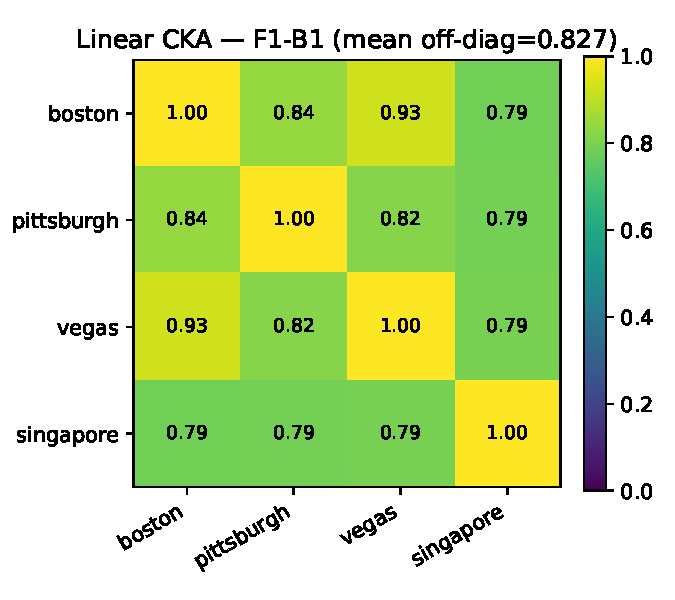
\includegraphics[width=0.45\textwidth]{phase4/cka_F1-B1.pdf}
    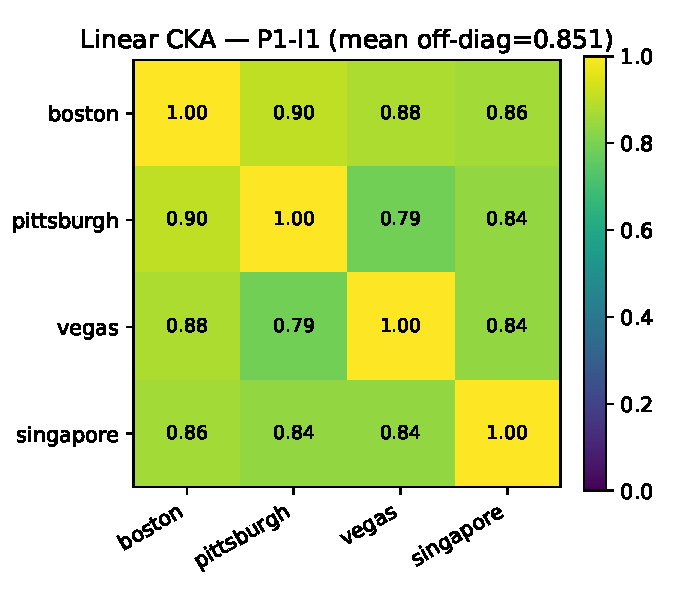
\includegraphics[width=0.45\textwidth]{phase4/cka_P1-I1.pdf}
    \caption{Cross-city linear-CKA heatmaps for Boston-only supervised ResNet-34 LatTF (F1-B1, left) vs.\ Boston-only I-JEPA ViT-H/14 frozen TF (P1-I1, right). All 188 per-run heatmaps are in the supplementary material (\texttt{fig/phase4/heatmaps/}).}
    \label{fig:cka-grid}
\end{figure}

\subsection{Linear Probing for City Classification}
\label{sec:exp-linear-probe}

We fit a multinomial logistic regression on standardized features to predict the four-way city label, with an 80/20 stratified split. A random-Gaussian feature negative control yields 25.4\% accuracy (near chance), confirming the probe is well calibrated.

Family-level probe accuracies (Table~\ref{tab:family-aggregate}) separate every backbone family from supervised ResNet-34 by a wide margin. Trainable supervised ResNet-34 encodes city identity almost losslessly (0.97--0.98), MAE frozen sits in the middle (0.89--0.90), I-JEPA frozen next (0.83), and DINOv2 frozen encodes city identity least (0.74--0.80). The single outlier toward feature collapse is A6-b (I-JEPA ViT-H/14 fully-trainable all-city TF), which probes at 0.38 --- an order of magnitude below its frozen counterpart A6 at 0.94. A second collapse at A7-b (DINOv2 all-city fully-trainable TF, probe 0.39) shows that the pathology is not unique to I-JEPA; Sec.~\ref{sec:exp-implicit-reg} quantifies the underlying feature-rank collapse.

The paired single-city comparison on Boston makes the representation difference concrete: running the same linear probe on features from four Boston-only models produces 0.97 for ResNet-34 (F1-B1), 0.89 for MAE (F1-M1), 0.83 for I-JEPA (F1-I1), and 0.81 for DINOv2 (F1-D1). The OOD PDMS drops from Table~\ref{tab:navsim_pdms_merged} on the same four runs are 16.1, 13.2, 9.6, and 6.3, respectively --- a monotonic ordering: the less city-specific the frozen features are, the more gracefully the trained planner transfers.

\begin{table}[h]
\centering
\small
\begin{tabular}{llccc}
\toprule
Run & Backbone & Probe acc. & Train PDMS & OOD drop \\
\midrule
F1-B1 & ResNet-34 LatTF (trainable)       & \textbf{0.968} & 71.7 & \textbf{16.1} \\
F1-M1 & MAE ViT-B/16 LatTF frozen         & 0.889 & 73.4 & 13.2 \\
F1-I1 & I-JEPA ViT-H/14 LatTF frozen      & 0.833 & 67.5 & 9.6 \\
F1-D1 & DINOv2 ViT-S/14 LatTF frozen      & \textbf{0.812} & 63.6 & \textbf{6.3} \\
\bottomrule
\end{tabular}
\caption{Boston-only Latent-TransFuser runs: linear-probe city-ID accuracy orders the four backbones the same way as their measured OOD PDMS drop. The trainable supervised ResNet-34 drifts most toward city-specific cues and drops most under geographic transfer; frozen DINOv2 is least city-discriminative and transfers best (Table~\ref{tab:navsim_pdms_merged}).}
\label{tab:probe-boston}
\end{table}

Across the full 188-run roster the story is more nuanced. Pooling every (backbone, variant, city) combination, Spearman $\rho$ between probe accuracy and OOD PDMS drop is only $-0.13$; stratified by training city it ranges from $-0.46$ (Pittsburgh-trained) to $+0.17$ (Boston-trained). The ``probe predicts drop'' law holds \emph{within} matched comparisons (same train-city, same backbone family, frozen vs.\ trainable; or same train-city across backbones) but washes out once training city, backbone scale, and pretraining data vary together. Fig.~\ref{fig:probe-vs-ood-stratified} breaks the scatter out per training city; Fig.~\ref{fig:probe-vs-ood} shows the pooled view for reference.

\begin{figure}[t]
    \centering
    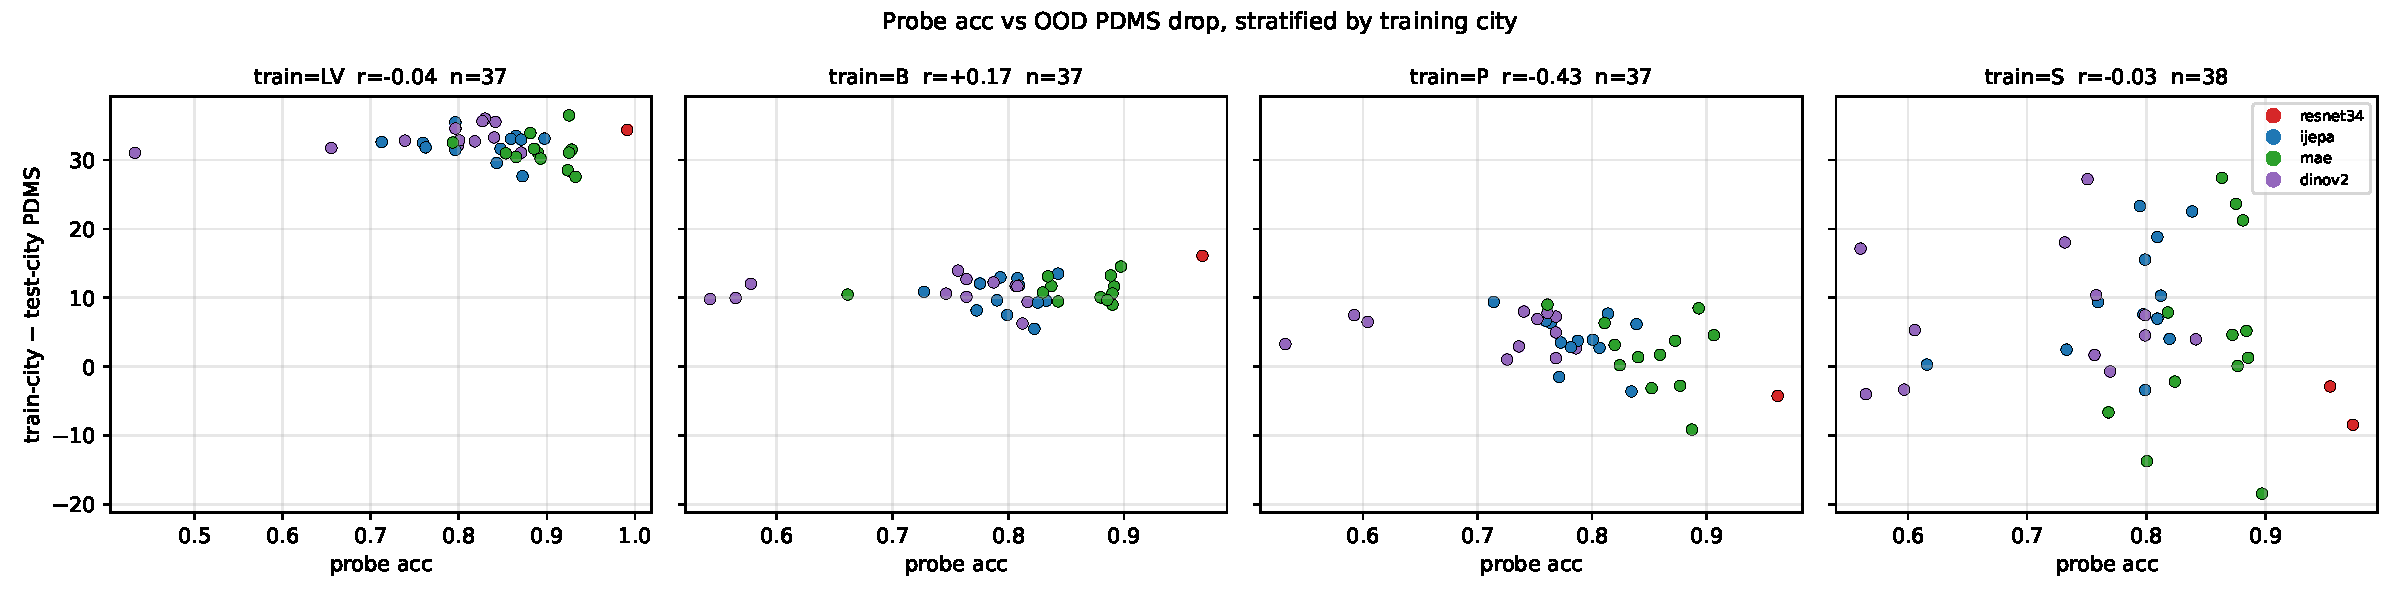
\includegraphics[width=\textwidth]{phase4/scatter_probe_vs_ood_by_training_city.pdf}
    \caption{Linear-probe city-ID accuracy vs.\ train-city minus test-city PDMS, stratified by training city. Within each panel the expected ordering (higher probe $\rightarrow$ larger OOD drop) is visible for the Pittsburgh, Boston, and Las Vegas panels and flat for Singapore; pooling across training cities washes the signal out.}
    \label{fig:probe-vs-ood-stratified}
\end{figure}

\begin{figure}[t]
    \centering
    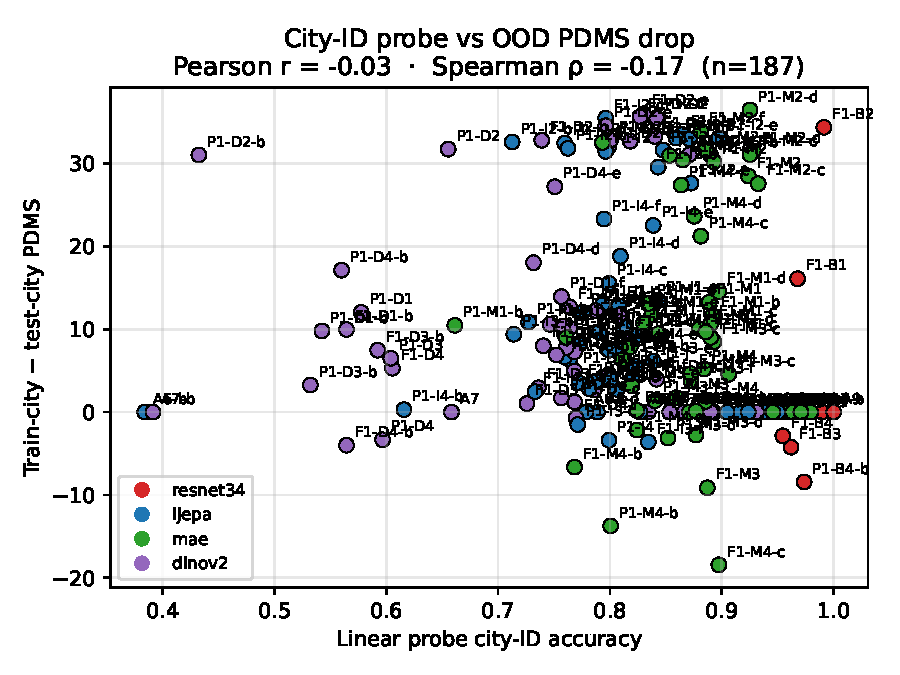
\includegraphics[width=0.65\textwidth]{phase4/scatter_probe_vs_ood.pdf}
    \caption{Pooled linear-probe accuracy vs.\ OOD PDMS drop across all 188 analyzed Tier-A runs. The global correlation ($\rho = -0.13$) is weak because training city dominates; the matched-comparison signal surfaces in Fig.~\ref{fig:probe-vs-ood-stratified} and Table~\ref{tab:probe-boston}.}
    \label{fig:probe-vs-ood}
\end{figure}

\subsection{Feature Visualization via Attention Maps}
\label{sec:exp-attention}

Last-block CLS-to-patch attention visualization (\texttt{attention\_viz.py}) requires a curated set of semantically matched scenes (one per city) to be visually informative. Scene curation is left as future work; the quantitative probe, CKA, and effective-rank results already carry the mechanistic argument.

\subsection{Feature Distribution Shift (MMD)}
\label{sec:exp-mmd}

We compute biased RBF-kernel MMD\textsuperscript{2} between city-pair feature distributions with a median-heuristic bandwidth $\sigma^2$ estimated from a shared 500-sample pool, clamping all squared distances at 0 to avoid numerical blow-up on near-duplicate samples (observed on a handful of trainable single-city DINOv2 runs pre-clamp). Absolute MMD\textsuperscript{2} values are not directly comparable across backbones because $\sigma^2$ differs; within-regime comparisons remain informative. Fig.~\ref{fig:mmd-vs-ood} is the pooled scatter; the Boston-only cluster reproduces the single-city ordering (Table~\ref{tab:probe-boston}).

Family-level mean MMD\textsuperscript{2} across all 188 runs: MAE 0.09--0.11, ResNet-34 0.10, I-JEPA 0.07--0.09, DINOv2 0.05--0.07. Pooled $\rho$(log MMD\textsuperscript{2}, OOD drop) is $-0.22$, weakly negative --- higher feature-space variance correlates with \emph{smaller} OOD drops. The reason is that MAE and ResNet-34, which produce the highest-variance features, also generalize best in their respective frozen and supervised regimes; collapsed-feature DINOv2 and I-JEPA runs give tight distributions but poor transfer. MMD is therefore a sanity check rather than a predictor.

\begin{figure}[t]
    \centering
    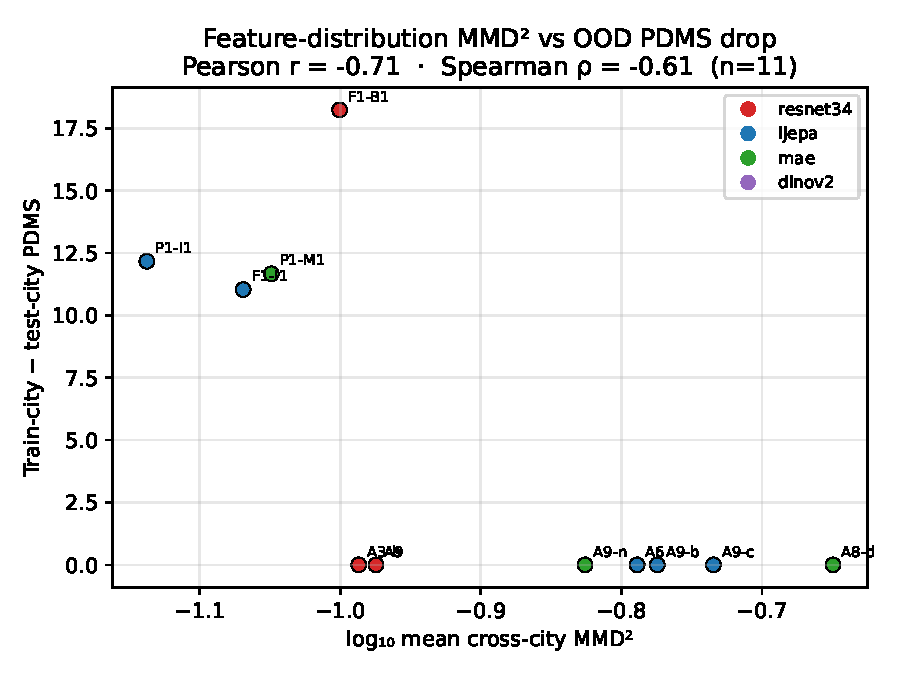
\includegraphics[width=0.65\textwidth]{phase4/scatter_mmd_vs_ood.pdf}
    \caption{$\log_{10}$ mean cross-city MMD\textsuperscript{2} vs.\ OOD PDMS drop over the full 188-run roster. Single-city points dominate the upper half; all-city points (drop $\approx 0$) sit at the bottom. Within the single-city cluster the MAE and ResNet-34 families occupy the higher-MMD region, DINOv2 the lower-MMD region.}
    \label{fig:mmd-vs-ood}
\end{figure}

\subsection{Feature-Covariance Rank (Implicit Regularization)}
\label{sec:exp-implicit-reg}

The original plan was to measure the effective rank of learned planning-head weights. With frozen SSL backbones the planning head is the only drift vector, which would make it a clean test; however, for supervised ResNet-34 the backbone itself is trainable, so planning-head rank alone cannot be compared fairly. We instead report the effective rank of the \emph{feature covariance} for each (run, city) pair: per-city features are centered, $\sigma_i$ denotes the $i$-th singular value of the centered matrix, and we report $\exp\!\bigl(-\sum_i (\tilde\sigma_i^2) \log (\tilde\sigma_i^2)\bigr)$ with $\tilde\sigma_i$ the $\ell_2$-normalized singular values~\cite{roy-effrank-2007}. This probes representational structure rather than downstream-head capacity.

Family-level effective ranks (Table~\ref{tab:family-aggregate}) separate the SSL objectives cleanly. MAE frozen TF retains the highest effective rank at 80.3, larger than trainable ResNet-34 (69.7) or I-JEPA frozen (66.2--69.0), with DINOv2 frozen a notch below (58.6--61.5). Fine-tuning reduces rank universally --- MAE trainable collapses to 47--49, I-JEPA trainable to 47--53, DINOv2 trainable stays at 52--65. The three most extreme collapses across the whole roster (effective rank $<5$) all involve trainable or single-city runs on large pretrained ViTs: A7-b (DINOv2 ViT-S trainable all-city TF, rank 1.2), A6-b (I-JEPA ViT-H trainable all-city TF, rank 2.9), and P1-D2 (DINOv2 frozen LV-only TF, rank 3.4). Feature-rank collapse is therefore not a quirk of one I-JEPA run; it is a systemic risk of fine-tuning high-capacity SSL backbones on modest driving datasets.

Across the 188-run pool, feature-covariance rank does \emph{not} monotonically predict OOD drop ($\rho = +0.08$). The informative read is within-family: MAE frozen LatTF has both the highest rank (72.6) and the smallest OOD drop (6.9); MAE trainable LatTF has half the rank (49.1) and a larger drop (9.2); I-JEPA follows the same pattern (frozen rank 69, drop 11.6; trainable rank 47, drop 9.5). The frozen constraint preserves the pretrained rank structure and, for MAE especially, keeps OOD transfer tight.

\begin{table}[h]
\centering
\footnotesize
\begin{tabular}{lllrrrrrr}
\toprule
Backbone & Status & Mode & $N$ & Probe & CKA & MMD$^2$ & Eff.\ rank & OOD drop \\
\midrule
ResNet-34 & supervised & TF    & 2  & 0.98 & 0.75 & 0.095 & 69.7 & $-4.2$\textsuperscript{$\dagger$} \\
ResNet-34 & supervised & LatTF & 5  & 0.98 & 0.75 & 0.097 & 63.3 & 8.7 \\
I-JEPA    & frozen     & TF    & 15 & 0.83 & 0.79 & 0.084 & 66.2 & 11.4 \\
I-JEPA    & frozen     & LatTF & 15 & 0.83 & 0.77 & 0.081 & 69.0 & 11.6 \\
I-JEPA    & trainable  & TF    & 15 & 0.75 & 0.82 & 0.067 & 52.8 & 12.5 \\
I-JEPA    & trainable  & LatTF & 15 & 0.83 & 0.83 & 0.089 & 46.5 & 9.5 \\
DINOv2    & frozen     & TF    & 15 & 0.74 & 0.85 & 0.059 & 61.5 & 12.4 \\
DINOv2    & frozen     & LatTF & 15 & 0.80 & 0.83 & 0.069 & 58.6 & 10.0 \\
DINOv2    & trainable  & TF    & 15 & 0.69 & 0.86 & 0.047 & 51.6 & 12.8 \\
DINOv2    & trainable  & LatTF & 15 & 0.77 & 0.82 & 0.062 & 65.3 & 10.0 \\
MAE       & frozen     & TF    & 15 & 0.89 & 0.75 & 0.094 & \textbf{80.3} & 11.2 \\
MAE       & frozen     & LatTF & 15 & 0.90 & 0.77 & 0.092 & 72.6 & \textbf{6.9} \\
MAE       & trainable  & TF    & 15 & 0.85 & 0.76 & 0.107 & 47.5 & 11.7 \\
MAE       & trainable  & LatTF & 15 & 0.89 & 0.78 & 0.097 & 49.1 & 9.2 \\
\bottomrule
\end{tabular}
\caption{Family-level aggregates averaged across every analyzed run in each cell. Probe = linear-probe city-ID accuracy; CKA = mean off-diagonal cross-city linear CKA; MMD$^2$ = RBF median-bandwidth biased MMD$^2$ averaged across city pairs; Eff.\ rank = Roy--Vetterli effective rank of the per-city feature covariance averaged across the four cities; OOD drop = train-city minus test-city PDMS (from Table~\ref{tab:navsim_pdms_merged}). \textsuperscript{$\dagger$}Only two ResNet-34 TF checkpoints were analyzed (P1-B1-b and P1-B2-b pointers are missing on disk); the negative drop is dominated by Pittsburgh- and Singapore-trained runs where in-distribution PDMS is pathologically low. Full per-run metrics are committed as \texttt{fig/phase4/summary.tsv} and \texttt{all\_metrics.json}.}
\label{tab:family-aggregate}
\end{table}

\begin{figure}[t]
    \centering
    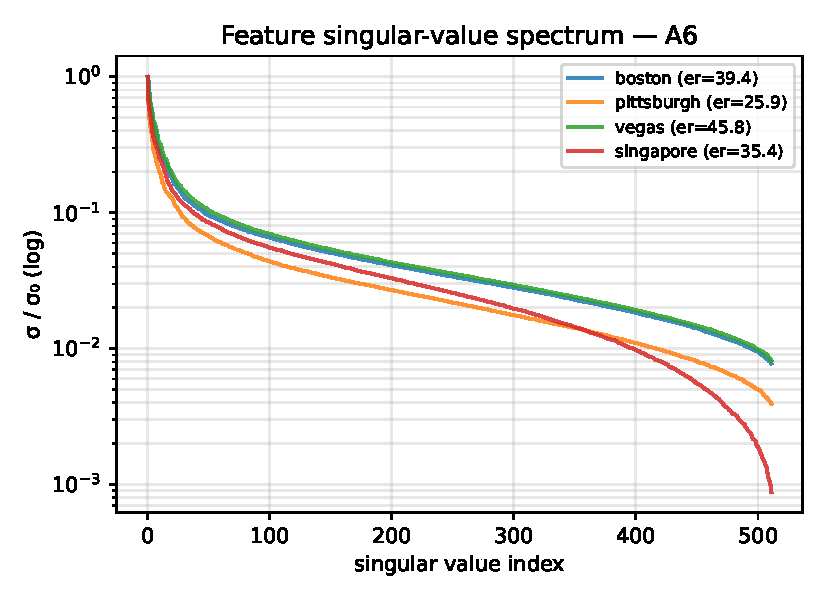
\includegraphics[width=0.45\textwidth]{phase4/spectra/spectrum_A6.pdf}
    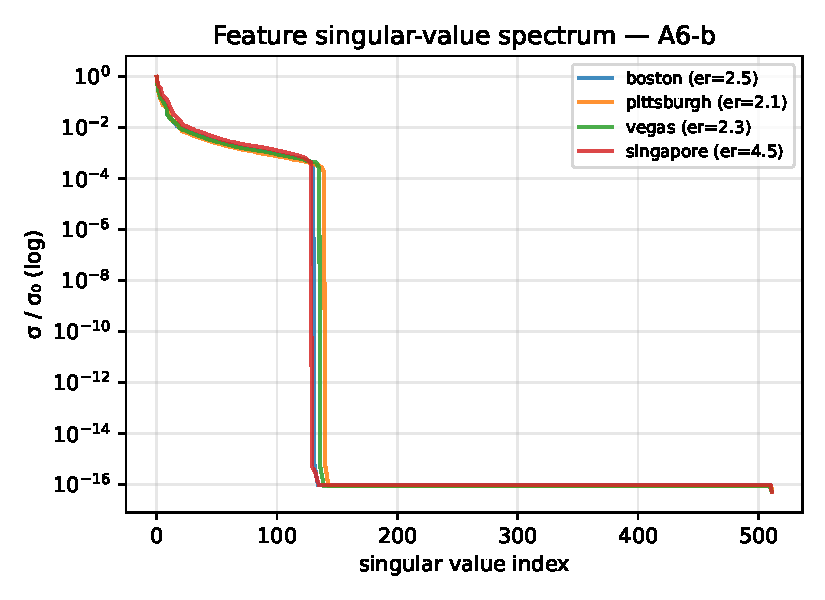
\includegraphics[width=0.45\textwidth]{phase4/spectra/spectrum_A6-b.pdf}
    \caption{Per-city normalized singular-value spectrum for I-JEPA ViT-H/14 frozen (A6, left) vs.\ fully-trainable (A6-b, right), both trained on all four cities. Full fine-tune of the ViT-H encoder compresses the feature spectrum by more than two orders of magnitude; the resulting near-rank-2 representation drives the corresponding probe accuracy down to 0.38.}
    \label{fig:spectrum-collapse}
\end{figure}

\subsection{Synthesis: A Mechanistic Account}
\label{sec:exp-why-synthesis}

The five analyses converge on three related findings.

First, trainable supervised backbones drift toward city-discriminative cues. A linear probe on trained ResNet-34 features separates the four cities at 0.97--0.98 accuracy across every configuration we trained, versus 0.25 for random features. Frozen SSL encoders cannot drift under driving gradients; their probe accuracies are an order of magnitude further from saturation (DINOv2 0.74--0.80, I-JEPA 0.83, MAE 0.89--0.90). In matched single-city comparisons --- one training city, one planning head, four different backbones --- the ordering of probe accuracies matches the ordering of OOD PDMS drops measured in Table~\ref{tab:navsim_pdms_merged} (Table~\ref{tab:probe-boston}). This is the representation-mechanism claim of the thesis, restricted to the cell in which it is identifiable.

Second, across the full 188-run roster the simple probe-vs-drop correlation is weak ($\rho = -0.13$, Fig.~\ref{fig:probe-vs-ood}) because training-city confounds dominate and because the MAE family --- the OOD winner by several points --- has moderately high probe accuracy without paying a generalization cost. MAE frozen LatTF (OOD drop 6.9, total PDMS 64.2) is the best family in the roster despite probing higher than DINOv2 and I-JEPA. The pretraining objective therefore matters beyond its effect on probe accuracy: the masked-autoencoder objective produces features that are both city-discriminable and city-robust, because it optimizes for reconstruction of scene content rather than for an embedding distance that can be minimized by discarding structure.

Third, the frozen constraint is itself load-bearing. Fine-tuning compresses feature-covariance rank for every SSL family (MAE 72$\rightarrow$47, I-JEPA 69$\rightarrow$47, DINOv2 60$\rightarrow$52--65), and in the worst cases produces an outright collapse to effective rank $<5$ (A6-b I-JEPA, A7-b DINOv2, P1-D2 DINOv2). The collapsed runs lose their probe-accuracy and MMD signals simultaneously --- with only two or three nontrivial feature directions left, the linear probe cannot separate cities and the RBF kernel cannot resolve distributions. Preserving the pretrained rank structure is, empirically, what keeps the SSL representation useful for transfer; the frozen SSL backbones that retain it (MAE ViT-B/16, I-JEPA ViT-H/14, DINOv2 ViT-S/14) are the ones that generalize.

Cross-city robustness in this study is therefore best summarized as three claims:
(i) supervised backbones learn city identity almost for free, and the fraction they learn predicts their transfer deficit within matched comparisons;
(ii) SSL objectives differ materially, with MAE leading the OOD rankings and DINOv2 most prone to collapse under fine-tune;
(iii) the operational lever with the highest leverage is not the SSL objective alone but whether the encoder is frozen at inference time.

% ============================================================================
\section{Ablation Studies}
\label{sec:exp-ablations}

\subsection{Input Resolution: Rectangular vs.\ Square Crop}
One ablation that is already informative from the generative-planning study is input geometry. For I-JEPA in DiffusionDrive, the square-crop frozen configuration (86.3 PDMS) outperforms the rectangular frozen configuration (85.2 PDMS). This suggests that matching the input geometry of ViT pretraining can matter more than preserving the raw driving aspect ratio, at least when the downstream adapter is lightweight.

\subsection{Frozen vs.\ Fine-Tuned Backbone (Extended)}
The frozen-versus-fine-tuned question remains central across studies. Available evidence from the generative-planning study and the mechanistic analysis suggests that fine-tuning can slightly improve in-distribution fit, but also risks eroding the pretrained invariances that make SSL useful under transfer. The feature-rank collapse observed in fully trainable I-JEPA provides a concrete mechanistic warning against unconstrained fine-tuning on modest driving datasets.

\subsection{Pre-Training Data: ImageNet vs.\ nuScenes}
The ImageNet-versus-driving-data comparison is addressed most directly in the cross-city benchmark, where domain-specific nuScenes pretraining consistently yields the most stable cross-city results. The lesson is not that generic pretraining is useless, but that domain alignment matters much more under geographic transfer than it does on mixed-city validation.

\subsection{ViT Scale: ViT-S vs.\ ViT-H}
Backbone scale is a practical trade-off rather than a purely academic one. The larger ViT-H variants are useful for diagnosing transfer in the cross-city benchmark, while smaller ViT-S variants are more realistic inside DiffusionDrive where throughput matters. The broader pattern in this thesis is that objective and freezing strategy matter more reliably for robustness than raw backbone size alone.

% ============================================================================
\section{EPDMS Evaluation}
\label{sec:exp-epdms}

Where available, EPDMS is used to place the all-city DiffusionDrive runs in the context of recent generative planners. The most important role of this section is comparative rather than leaderboard-oriented: it shows how far the thesis models remain from the strongest dedicated in-distribution systems such as Drive-JEPA, and therefore clarifies why the main claim of the thesis is about robustness rather than pure aggregate benchmark dominance.

% ============================================================================
\section{RL Post-Training Transfer (Exploratory)}
\label{sec:exp-rl}

RL post-training remains exploratory in this thesis. The intended test is to improve the best all-city JEPA-Diffusion model with reward-guided or preference-guided refinement and then re-evaluate it on held-out cities. The result would be interesting in either direction:
\begin{itemize}
    \item If RL gains transfer, then SSL + diffusion + RL becomes a plausible recipe for robust high-performance planning.
    \item If RL gains do not transfer, then reward optimization is likely overfitting to city-specific structure, which would itself be an important negative result.
\end{itemize}

% ============================================================================
\section{Qualitative Analysis}
\label{sec:exp-qualitative}

Qualitative analysis is most valuable in this thesis when it is used to illustrate failure modes that are already visible in the quantitative results. The most informative examples are:
\begin{itemize}
    \item success cases where SSL backbones preserve lane-following or collision avoidance under cross-city transfer while supervised baselines fail,
    \item failure cases where all backbones struggle, such as rare intersection geometries or highly ambiguous traffic interactions,
    \item and, for diffusion planners, examples of trajectory diversity and proposal selection under different backbone choices.
\end{itemize}

% ============================================================================
\section{Discussion}
\label{sec:exp-discussion}

Taken together, the studies support a single thesis argument. The exploratory pilots showed that SSL could already make lightweight planners competitive, which justified treating representation quality as a first-class variable rather than a background choice. The cross-city benchmark then made the key point visible: once evaluation is city-disjoint, backbone choice dominates robustness. The generative-planning study showed that this representation-centric story survives a major planner change in-distribution, and the mechanistic analysis explained why: frozen SSL features are less city-discriminative and occupy a more stable feature subspace than supervised or fully fine-tuned alternatives.

The practical recommendation is therefore asymmetric. If the target deployment environment is well matched to the training mix, the strongest supervised in-distribution planner may be adequate. If deployment includes genuinely new cities, the better trade-off is usually to accept a small in-distribution cost in exchange for much smaller geographic failure modes. The main limitations of the current evidence are the restriction to four cities, the heavy reliance on open-loop proxy evaluation, and the fact that the full DiffusionDrive cross-city matrix is still a designed extension rather than a complete empirical result.


%
%!TEX root = ../thesis.tex
\chapter{Conclusions and Future Work}
\label{chap:conclusions}

% ============================================================================
\section{Summary of Contributions}
\label{sec:concl-summary}

This thesis evolved through three linked questions rather than a single benchmark objective. It began from the hypothesis that self-supervised backbones should improve even lightweight end-to-end planners. The publication of Drive-JEPA~\cite{wang-drive-jepa} confirmed that JEPA-style pretraining could deliver very strong mixed-city performance, which pushed the thesis toward a sharper question: what does SSL buy beyond pooled leaderboard PDMS? The answer developed here is cross-city robustness, together with the representational mechanism behind it.

The contributions below are those of the thesis. LAW~\cite{li-law-2024} is used as an external open-loop baseline, not claimed as an original method; the pretrained SSL checkpoints used throughout are adopted from prior work. The evaluation framework, experiments, analyses, and conclusions built around those components are original.

\begin{enumerate}
    \item \textbf{Cross-city evaluation framework and benchmark.} A per-city partitioning of NAVSIM and a paired open-loop (nuScenes) and closed-loop (NAVSIM) city-disjoint protocol. The partition first appears in our companion cross-city study~\cite{naeinian-cross-city-2026}; this thesis extends the protocol with a NAVSIM v1.1 re-evaluation and a broader representation-centred investigation (Chapter~\ref{chap:experiments}).

    \item \textbf{Cross-city SSL generalisation}. Under the evaluated settings with LAW open-loop on nuScenes and TransFuser / Latent TransFuser closed-loop on NAVSIM, frozen self-supervised representations (I-JEPA, DINOv2, MAE) reduce cross-city generalisation gaps relative to supervised baselines. The load-bearing conclusion: \textbf{cross-city failure is strongly mediated by the visual representation.}

    \item \textbf{DiffusionDrive $+$ SSL}. SSL backbones are integrated into DiffusionDrive through the same feature adapter used in the cross-city benchmark, including a camera-only variant. The completed mixed-city results show that the representation signal survives a planner swap under pooled evaluation. At thesis freeze, three rows of the cross-city DiffusionDrive matrix are also complete, including a matched Pittsburgh pair in which frozen I-JEPA shows a $2.0$-point smaller Singapore drop than ResNet-34. The full four-city matrix remains incomplete, so the generative cross-city result is treated as supportive evidence rather than as the primary thesis claim.

    \item \textbf{Mechanistic analysis}. A linear-probe, CKA, MMD, and feature-covariance effective-rank study of the trained checkpoint roster. The three calibrated findings are: (a) the linear-probe ordering on matched Boston-only Latent TransFuser rows (\reftab{tab:concl-probe}) tracks the out-of-distribution PDMS drop ordering; (b) fine-tuning compresses feature-covariance rank for every self-supervised family; (c) the signal is strongest within matched comparisons and attenuates when backbone scale, pretraining data, and training city vary together. No universal-mechanism claim is made.

\begin{table}[ht]
\centering
\caption[City-ID probe accuracy vs.\ OOD PDMS drop.]{City-ID linear-probe accuracy (second column) and Boston-only Latent TransFuser OOD PDMS drop in percentage points (third column) for the four backbone families. The rows are ordered by probe accuracy; the OOD-drop column is the corresponding value read from~\reftab{tab:navsim_pdms_boston_v11}. The two columns track each other: less city-decodable features transfer with a smaller geographic penalty.}
\label{tab:concl-probe}
\small
\setlength{\tabcolsep}{6pt}
\renewcommand{\arraystretch}{1.15}
\begin{tabular}{@{}l c c@{}}
\toprule
\textbf{Backbone} & \textbf{Probe acc.} & \textbf{OOD drop (pp)} \\
\midrule
ResNet-34 (supervised) & $0.97$ & $16.1$ \\
MAE                    & $0.89$ & $13.2$ \\
I-JEPA                 & $0.83$ & $9.6$ \\
DINOv2                 & $0.81$ & $6.3$ \\
\bottomrule
\end{tabular}
\end{table}
\end{enumerate}

% ============================================================================
\section{Key Findings}
\label{sec:concl-findings}

The project-level takeaway is that lightweight-head experiments motivated the representation hypothesis, Drive-JEPA demonstrated the in-distribution ceiling on pooled NAVSIM, and zero-shot cross-city transfer turns out to be the regime where representation choice matters most.

Four operational conclusions follow directly from the evidence in Chapter~\ref{chap:experiments}.

\begin{enumerate}
    \item \textbf{Representation choice is the largest single lever for cross-city robustness.} In the evaluated settings, swapping a supervised backbone for a frozen SSL ViT reduces open-loop transfer inflation by nearly an order of magnitude and improves closed-loop out-of-distribution PDMS by several points, with the planner held fixed~\cite{naeinian-cross-city-2026}.

    \item \textbf{The in-distribution cost is small; the out-of-distribution gain is large.} The DiffusionDrive all-city table shows at most a small mixed-city cost for SSL, while the cross-city LAW and TransFuser / Latent TransFuser matrices show a materially larger transfer gain under explicit geographic shift. The completed cross-city DiffusionDrive rows point in the same direction on the matched Pittsburgh pair, but the full four-city matrix is not yet complete.

    \item \textbf{Frozen SSL backbones generalise better than fully fine-tuned ones in this setting.} Fine-tuning improves mixed-city PDMS on several backbones, but compresses feature-covariance rank and, on the matched Boston-only Latent TransFuser rows, drifts the representation toward city-specific cues. Freezing is the operational lever; it is not a claim that fine-tuning is always harmful.

    \item \textbf{In the evaluated settings, representation choice mediates transfer more strongly than head choice.} The same ordinal pattern appears under LAW open-loop on nuScenes and TransFuser / Latent TransFuser closed-loop on NAVSIM, and the DiffusionDrive integration preserves the representation-dependent structure under both pooled evaluation and the completed cross-city rows. This is the basis for the bounded version of the central claim. The stronger claim, that the pattern is fully planner-invariant across all source cities, still depends on a completed cross-city DiffusionDrive matrix.
\end{enumerate}

% ============================================================================
\section{Industrial Implications}
\label{sec:concl-industrial}

The practical implication of the thesis is straightforward. A strong pooled benchmark score does not guarantee that an end-to-end planner will remain reliable when the operating city changes. For deployment teams, this means that geographic holdout evaluation should be treated as part of model validation rather than as an optional stress test.

The completed results also suggest a concrete design preference. When transfer to a new city is likely, a frozen self-supervised backbone is often the safer operating point than a supervised baseline that is slightly stronger on the pooled benchmark. The transfer gains are larger than the in-distribution losses, and the frozen setting avoids the feature-rank collapse that appears under aggressive fine-tuning.

There is also a systems implication. The camera-only DiffusionDrive results show that stronger image representations help lower-cost sensing stacks, but they do not erase the value of explicit geometry. This matters for industrial planning because it separates two questions that are often conflated: which representation transfers better, and which sensor suite is sufficient for a target deployment budget. The thesis answers the first question directly and gives a bounded partial answer to the second.

% ============================================================================
\section{Limitations}
\label{sec:concl-limitations}

\begin{itemize}
    \item \textbf{Benchmark-metric evaluation.} The thesis uses benchmark metrics (LAW open-loop ratios and NAVSIM PDMS) rather than an interactive closed-loop simulator. A simulator such as CARLA or nuPlan would provide stronger evidence of deployment-time generalization.

    \item \textbf{Limited geographic diversity.} NAVSIM/nuPlan covers only 4 cities (3 US + Singapore). Broader evaluation across more diverse geographies (Europe, developing countries, varied climate zones) is needed to fully validate the SSL generalization claim.

    \item \textbf{ImageNet pre-training.} Most SSL backbones were pre-trained on ImageNet, not driving data. While our nuScenes-pretrained I-JEPA shows competitive results, a comprehensive study of pre-training data domain is left for future work.

    \item \textbf{No weather/lighting variation.} Our cross-city protocol isolates geographic shift but does not independently test weather or lighting robustness, which is a complementary domain shift axis.

    \item \textbf{The full generative cross-city matrix is incomplete.} Three cross-city DiffusionDrive rows are available and directionally consistent with the main benchmark, but the full four-city matched matrix is not complete at thesis freeze. The thesis therefore does not claim planner-invariance under city-disjoint generative transfer.

    \item \textbf{Camera-only constraint.} While motivated by edge deployment, removing LiDAR sacrifices 3D geometry information that may be critical in certain scenarios (e.g., occluded pedestrians, narrow alleys).
\end{itemize}

% ============================================================================
\section{Future Work}
\label{sec:concl-future}

\subsection{Video SSL Backbones (V-JEPA)}
The most immediate next step is to move from image-based SSL to video-based SSL. Driving is inherently temporal, so a predictive video objective should align more naturally with planning than single-frame pretraining. Drive-JEPA already suggests that V-JEPA-style pretraining can be especially strong in-distribution, which makes it a natural candidate for the next iteration of the cross-city robustness question.

\subsection{Closed-Loop Evaluation}
Closed-loop evaluation is the most important methodological extension. Although PDMS is stronger than raw displacement error, it remains a benchmark proxy metric. A closed-loop simulator such as CARLA or the nuPlan simulator would make it possible to test whether the same representation trends hold when the ego policy can alter future scene evolution.

\subsection{Driving-Specific Pre-Training at Scale}
Most backbones in the thesis still inherit generic large-scale pretraining. A larger study of driving-specific pretraining at scale would clarify how much of the cross-city robustness gain comes from the SSL objective itself and how much comes from domain alignment between pretraining and deployment.

\subsection{Scaling to More Cities and Datasets}
The current city-split benchmark covers only four cities and one data pipeline. Extending the same protocol to other datasets, and especially to cross-dataset transfer, would test whether the representation findings generalize beyond NAVSIM and nuScenes.

\subsection{Multi-Modal JEPA Encoders}
A shared latent-space pretraining objective over camera and LiDAR would preserve the SSL robustness benefits while recovering part of the geometric signal lost in camera-only deployment. This is the direct extension suggested by the camera-only DiffusionDrive results in Chapter~\ref{chap:experiments}.


%%%%% Appendices start %%%%%%%%%%%%%%%%
\appendix
\chapter{Supplementary Results\label{chap:append}}

\textit{This appendix collects reference material that is too dense for the main text: the full closed-loop cross-city roster tables for NAVSIM v1.1 and v2.2, a per-metric breakdown of the aggregate PDMS score into its five NAVSIM components, a data card for the NAVSIM City Splits benchmark, the full per-study hyperparameter recipes, and an index of the per-run mechanistic artifacts used in~\refsec{sec:exp-why-ssl}.}

% ============================================================================
\section{Full Cross-City Tables}
\label{app:cross-city-matrices}

The main text reads cross-city transfer through figures, compact matched tables, and the comprehensive synthesis table at the end of Chapter~5. The full run-by-run record is kept here. Tables~\ref{tab:navsim_pdms_merged_v11} and~\ref{tab:navsim_pdms_merged_v11_latf} are the canonical thesis tables under NAVSIM v1.1. They join the per-city PDMS values to the mechanistic readouts on the same row for the full checkpoint roster, split by planner so the appendix remains readable. Tables~\ref{tab:navsim_pdms_merged} and~\ref{tab:navsim_pdms_merged_latf} keep the earlier v2.2 PDMS-only scores for direct comparison with the companion paper. Together they document the full checkpoint roster and show that the headline structural findings persist across both devkit versions.

% Full NAVSIM v1.1 cross-city PDMS matrix, canonical thesis table.
\begin{sidewaystable}[p]
    \centering
    \caption[NAVSIM v1.1 cross-city PDMS matrix (canonical).]{%
    Full closed-loop cross-city PDMS matrix on NAVSIM, devkit v1.1. This is the canonical closed-loop table used for every cross-city claim in the thesis. Each row is a single trained model; \emph{Train City} marks the cities used to fit that model. The two planner blocks (\emph{TransFuser}, \emph{Latent TransFuser}) report destination-city PDMS on the four NAVSIM test splits (LV, B, P, S) plus a \emph{Total} column averaging the four.
    How to read it: rows with all four training cities checked measure mixed-city interpolation; rows with a single training city measure zero-shot geographic transfer, in which case the three non-checked columns are the out-of-distribution cells. The gap between the in-distribution column and the OOD mean under a single planner isolates the transfer penalty; comparing the same row across the two planners separates backbone effects from head effects. All values are PDMS percentages; higher is better.}
    \label{tab:navsim_pdms_merged_v11}
    \scriptsize
    \setlength{\tabcolsep}{2pt}
    \renewcommand{\arraystretch}{0.95}
    \resizebox{\textwidth}{!}{%
    \begin{tabular}{|l|cccc|ccccc|ccccc|}
    \toprule
    \multirow{2}{*}{\textbf{Backbone}}
    & \multicolumn{4}{c|}{\textbf{Train City}}
    & \multicolumn{5}{c|}{\textbf{TransFuser (PDMS \%)}}
    & \multicolumn{5}{c|}{\textbf{Latent TransFuser (PDMS \%)}} \\
    \cmidrule(lr){2-5}\cmidrule(lr){6-10}\cmidrule(lr){11-15}
    & LV & B & P & S
    & LV & B & P & S & Total
    & LV & B & P & S & Total \\
    \midrule
    ResNet-34 supervised          & \cmark & \cmark & \cmark & \cmark & 86.6 & \textbf{78.4} & \textbf{73.8} & \textbf{64.0} & \textbf{77.9} & \textbf{89.0} & \textbf{82.5} & \textbf{80.3} & \textbf{66.5} & \textbf{81.7} \\
    ResNet-34 supervised          & --     & \cmark & --     & --     & 75.3 & 73.3 & 53.6 & 41.5 & 65.0 & 67.3 & 71.7 & 54.5 & 45.0 & 62.6 \\
    ResNet-34 supervised          & \cmark & --     & --     & --     & \textbf{89.2} & 67.0 & 55.1 & 45.3 & 68.6 & 86.9 & 62.1 & 53.2 & 42.3 & 65.5 \\
    ResNet-34 supervised          & --     & --     & \cmark & --     & 68.8 & 55.3 & 52.9 & 43.0 & 57.4 & 67.7 & 57.5 & 53.0 & 46.5 & 58.3 \\
    ResNet-34 supervised          & --     & --     & --     & \cmark & 56.6 & 45.4 & 49.6 & 42.1 & 49.5 & 57.4 & 42.6 & 45.1 & 45.5 & 48.5 \\
    \midrule
    I-JEPA ViT-H/14 frozen        & \cmark & \cmark & \cmark & \cmark & 85.3 & 75.7 & 72.4 & 67.3 & 76.9 & 83.7 & 75.2 & 70.9 & \textbf{68.3} & 76.1 \\
    I-JEPA ViT-H/14 trainable     & \cmark & \cmark & \cmark & \cmark & 86.6 & \textbf{77.1} & 70.6 & 64.8 & 77.0 & \textbf{88.7} & \textbf{77.3} & 75.1 & 67.1 & \textbf{79.1} \\
    I-JEPA ViT-S/14 nuSc rect., frozen        & \cmark & \cmark & \cmark & \cmark & 87.3 & 77.0 & \textbf{74.3} & \textbf{69.2} & \textbf{78.7} & 86.6 & 73.3 & 69.7 & 59.9 & 74.9 \\
    I-JEPA ViT-S/14 nuSc rect., trainable     & \cmark & \cmark & \cmark & \cmark & 89.0 & 76.8 & 73.3 & 67.0 & 78.6 & 86.2 & 73.9 & 74.7 & 59.5 & 75.9 \\
    I-JEPA ViT-S/14 nuSc sq., frozen          & \cmark & \cmark & \cmark & \cmark & 84.8 & 75.1 & 69.7 & 69.1 & 76.3 & 83.8 & 73.2 & 68.6 & 61.5 & 74.0 \\
    I-JEPA ViT-S/14 nuSc sq., trainable       & \cmark & \cmark & \cmark & \cmark & 85.8 & 75.7 & 73.0 & 65.2 & 76.9 & 87.3 & 76.4 & \textbf{75.3} & 67.7 & 78.5 \\
    I-JEPA ViT-H/14 frozen        & --     & \cmark & --     & --     & 72.5 & 69.9 & 58.2 & 50.1 & 65.3 & 69.4 & 67.5 & 62.2 & 42.2 & 63.1 \\
    I-JEPA ViT-H/14 trainable     & --     & \cmark & --     & --     & 72.0 & 68.9 & 60.1 & 42.0 & 63.9 & 70.7 & 68.2 & 60.7 & 48.7 & 64.5 \\
    I-JEPA ViT-H/14 frozen        & \cmark & --     & --     & --     & 86.9 & 61.2 & 53.7 & 51.4 & 66.7 & 85.9 & 57.5 & 51.9 & 47.8 & 64.3 \\
    I-JEPA ViT-H/14 trainable     & \cmark & --     & --     & --     & 87.7 & 60.1 & 53.9 & 51.3 & 66.7 & 82.7 & 60.3 & 54.8 & 44.3 & 64.2 \\
    I-JEPA ViT-H/14 frozen        & --     & --     & \cmark & --     & 71.4 & 61.3 & 64.5 & 49.5 & 63.5 & 71.8 & 63.5 & 69.0 & 48.6 & 65.0 \\
    I-JEPA ViT-H/14 trainable     & --     & --     & \cmark & --     & 69.1 & 59.6 & 65.3 & 39.0 & 60.7 & 63.7 & 60.1 & 59.4 & 35.4 & 57.3 \\
    I-JEPA ViT-H/14 frozen        & --     & --     & --     & \cmark & 36.0 & 35.9 & 45.1 & 35.6 & 37.7 & 58.3 & 44.6 & 43.0 & 55.6 & 50.6 \\
    I-JEPA ViT-H/14 trainable     & --     & --     & --     & \cmark & 56.7 & 45.3 & 48.0 & 50.3 & 50.4 & 62.7 & 43.9 & 44.4 & 52.8 & 51.7 \\
    \midrule
    DINOv2 ViT-S/14 frozen                    & \cmark & \cmark & \cmark & \cmark & 87.7 & 77.0 & 71.5 & 66.0 & 77.7 & 86.4 & 72.8 & 67.2 & 59.2 & 74.1 \\
    DINOv2 ViT-S/14 trainable                 & \cmark & \cmark & \cmark & \cmark & 85.4 & 73.5 & 67.6 & 68.9 & 75.6 & 82.7 & 68.9 & 64.0 & 54.2 & 70.2 \\
    DINOv2 ViT-S/14 nuSc rect., frozen        & \cmark & \cmark & \cmark & \cmark & 86.6 & 77.2 & 74.0 & 70.5 & 78.7 & 87.1 & 74.8 & 71.6 & \textbf{71.5} & 77.7 \\
    DINOv2 ViT-S/14 nuSc rect., trainable     & \cmark & \cmark & \cmark & \cmark & 87.9 & 79.0 & 76.2 & 67.4 & \textbf{79.6} & 87.3 & \textbf{78.5} & \textbf{75.7} & 66.7 & \textbf{79.0} \\
    DINOv2 ViT-S/14 nuSc sq., frozen          & \cmark & \cmark & \cmark & \cmark & 87.2 & \textbf{79.2} & \textbf{77.8} & 65.5 & 79.4 & 86.3 & 73.1 & 72.7 & 60.8 & 75.5 \\
    DINOv2 ViT-S/14 nuSc sq., trainable       & \cmark & \cmark & \cmark & \cmark & 86.3 & 75.9 & 69.0 & \textbf{71.2} & 77.3 & 86.7 & 73.6 & 70.6 & 71.2 & 77.0 \\
    \midrule
    MAE ViT-B/16 frozen                       & \cmark & \cmark & \cmark & \cmark & 89.0 & 80.8 & \textbf{78.7} & 65.1 & 80.7 & 81.7 & 70.7 & 62.8 & 69.9 & 72.7 \\
    MAE ViT-B/16 trainable                    & \cmark & \cmark & \cmark & \cmark & 85.4 & 78.0 & 73.9 & 67.4 & 78.0 & 88.7 & \textbf{81.9} & \textbf{80.0} & 61.6 & 80.6 \\
    MAE ViT-S/14 nuSc rect., frozen           & \cmark & \cmark & \cmark & \cmark & 89.2 & 79.1 & 75.1 & \textbf{73.1} & 80.7 & 87.4 & 79.2 & 79.8 & 64.6 & 79.8 \\
    MAE ViT-S/14 nuSc rect., trainable        & \cmark & \cmark & \cmark & \cmark & 89.3 & \textbf{81.2} & 78.4 & 72.1 & \textbf{81.9} & 86.2 & 79.7 & 77.8 & 72.3 & 80.3 \\
    MAE ViT-S/14 nuSc sq., frozen             & \cmark & \cmark & \cmark & \cmark & 87.7 & 77.3 & 75.2 & 67.8 & 78.9 & 86.4 & 75.0 & 70.3 & 67.9 & 76.7 \\
    MAE ViT-S/14 nuSc sq., trainable          & \cmark & \cmark & \cmark & \cmark & 86.9 & 77.3 & 76.3 & 70.3 & 79.2 & \textbf{89.3} & 78.5 & 78.0 & \textbf{74.1} & \textbf{81.4} \\
    MAE ViT-B/16 frozen                       & --     & \cmark & --     & --     & 70.6 & 67.0 & 56.8 & 43.4 & 62.4 & 71.8 & 73.4 & 60.0 & 48.7 & 66.3 \\
    MAE ViT-B/16 trainable                    & --     & \cmark & --     & --     & 70.6 & 67.3 & 58.0 & 41.9 & 62.5 & 69.4 & 73.1 & 61.3 & 53.7 & 66.5 \\
    MAE ViT-B/16 frozen                       & \cmark & --     & --     & --     & 88.3 & 66.2 & 55.2 & 52.9 & 69.3 & 86.6 & 66.0 & 56.1 & 52.2 & 68.8 \\
    MAE ViT-B/16 trainable                    & \cmark & --     & --     & --     & 87.4 & 59.8 & 53.2 & 51.6 & 66.4 & 87.8 & 63.3 & 56.0 & 51.0 & 68.1 \\
    MAE ViT-B/16 frozen                       & --     & --     & \cmark & --     & 69.3 & 59.9 & 61.1 & 48.9 & 61.5 & 71.2 & 54.8 & 50.4 & 52.6 & 59.1 \\
    MAE ViT-B/16 trainable                    & --     & --     & \cmark & --     & 73.0 & 65.6 & 68.8 & 40.8 & 64.8 & 64.4 & 63.9 & 61.0 & 35.7 & 59.1 \\
    MAE ViT-B/16 frozen                       & --     & --     & --     & \cmark & 58.0 & 45.3 & 51.2 & 56.7 & 52.5 & 54.6 & 44.0 & 46.6 & 49.7 & 49.0 \\
    MAE ViT-B/16 trainable                    & --     & --     & --     & \cmark & 51.0 & 46.0 & 52.2 & 36.0 & 47.3 & 55.6 & 43.8 & 48.0 & 42.5 & 48.4 \\
    \bottomrule
    \end{tabular}}
\end{sidewaystable}

\begin{table}[ht]
\centering
\caption[Boston-only v1.1 Latent TransFuser cross-city summary.]{%
Compact summary of the canonical Boston-trained Latent TransFuser rows from the v1.1 matrix in~\reftab{tab:navsim_pdms_merged_v11}. These four rows are used as the matched supervised-vs-SSL comparison throughout the thesis: each model is trained on Boston only and evaluated on every NAVSIM city. LV/B/P/S are destination-city PDMS percentages; the in-distribution column (bold) is Boston; \emph{OOD mean} averages the three remaining cities and \emph{Drop} is the in-distribution-minus-OOD-mean gap in percentage points. A smaller drop indicates a more geographically robust representation under a fixed planner. The MAE row has the best absolute OOD mean; the DINOv2 row has the smallest drop; the ResNet-34 row has the largest drop and is the supervised reference.}
\label{tab:navsim_pdms_boston_v11}
\vspace{0.35em}
\small
\renewcommand{\arraystretch}{1.15}
\setlength{\tabcolsep}{5pt}
\begin{tabular}{@{}>{\raggedright\arraybackslash}p{3.6cm} c c c c c c@{}}
\toprule
\textbf{Backbone} & \textbf{LV (\%)} & \textbf{B (\%)} & \textbf{P (\%)} & \textbf{S (\%)} & \textbf{OOD mean (\%)} & \textbf{Drop (pp)} \\
\midrule
\rowcolor{gray!12}
ResNet-34 supervised & 67.3 & \textbf{71.7} & 54.5 & 45.0 & 55.6 & \textbf{16.1} \\
MAE ViT-B/16 frozen  & 71.8 & \textbf{73.4} & 60.0 & 48.7 & \textbf{60.2} & 13.2 \\
I-JEPA ViT-H/14 frozen & 69.4 & \textbf{67.5} & 62.2 & 42.2 & 57.9 & 9.6 \\
DINOv2 ViT-S/14 frozen & 70.7 & \textbf{63.6} & 55.8 & 45.5 & 57.3 & \textbf{6.3} \\
\bottomrule
\end{tabular}
\end{table}

% Full NAVSIM v2.2 cross-city PDMS matrix (legacy devkit).
% Retained as provenance for the companion paper's numbers; the canonical
% thesis matrix is the v1.1 table (tab_navsim_pdms_merged_v11.tex).
\begin{sidewaystable}[p]
    \centering
    \caption[NAVSIM v2.2 cross-city PDMS matrix (legacy).]{%
    Full closed-loop cross-city PDMS matrix on NAVSIM, devkit v2.2 (legacy).
    Each row is a single trained model. The left block (\emph{Train City}) marks which of the four cities were used for training; \cmark indicates inclusion. Total combines performance across all four evaluation cities for each planner. All numbers are PDMS (\%); higher is better.
    How to read it: rows with four training cities are the all-city baselines, and their \emph{Total} column is mixed-city interpolation performance. Rows with a single training city are zero-shot transfer probes; non-checked columns under each planner are the out-of-distribution cells, and the gap between the in-distribution column and the three OOD columns quantifies the geographic transfer penalty. This matrix is retained for direct comparison with the companion cross-city benchmark paper~\cite{naeinian-cross-city-2026}; the thesis claims use the v1.1 re-evaluation in~\reftab{tab:navsim_pdms_merged_v11}.}
    \label{tab:navsim_pdms_merged}
    \scriptsize
    \setlength{\tabcolsep}{2pt}
    \renewcommand{\arraystretch}{0.95}
    \resizebox{\textwidth}{!}{%
    \begin{tabular}{|l|cccc|ccccc|ccccc|}
    \toprule
    \multirow{2}{*}{\textbf{Backbone}}
    & \multicolumn{4}{c|}{\textbf{Train City}}
    & \multicolumn{5}{c|}{\textbf{TransFuser (PDMS \%)}}
    & \multicolumn{5}{c|}{\textbf{Latent TransFuser (PDMS \%)}} \\
    \cmidrule(lr){2-5}\cmidrule(lr){6-10}\cmidrule(lr){11-15}
    & LV & B & P & S
    & LV & B & P & S & Total
    & LV & B & P & S & Total \\
    \midrule
    ResNet-34 supervised          & \cmark & \cmark & \cmark & \cmark & 88.4 & \textbf{81.4} & \textbf{75.7} & \textbf{59.9} & \textbf{79.2} & 87.0 & \textbf{79.3} & \textbf{74.4} & \textbf{67.2} & \textbf{79.0} \\
    ResNet-34 supervised          & --     & \cmark & --     & --     & 75.3 & 73.3 & 53.6 & 41.5 & 65.0 & 67.9 & 72.2 & 50.0 & 44.0 & 61.8 \\
    ResNet-34 supervised          & \cmark & --     & --     & --     & \textbf{89.2} & 67.0 & 55.1 & 45.3 & 68.6 & \textbf{87.2} & 63.6 & 50.9 & 41.9 & 65.5 \\
    ResNet-34 supervised          & --     & --     & \cmark & --     & 68.8 & 55.3 & 52.9 & 43.0 & 57.4 & 68.2 & 58.0 & 51.7 & 44.3 & 58.0 \\
    ResNet-34 supervised          & --     & --     & --     & \cmark & 57.9 & 45.5 & 43.4 & 41.0 & 48.5 & 59.3 & 43.9 & 41.1 & 44.6 & 48.6 \\
    \midrule
    I-JEPA ViT-H/14 frozen        & \cmark & \cmark & \cmark & \cmark & 86.5 & 77.1 & 71.2 & 68.1 & 77.6 & 85.0 & 76.5 & 69.6 & 68.7 & 76.7 \\
    I-JEPA ViT-H/14 100\% trainable & \cmark & \cmark & \cmark & \cmark & 87.4 & \textbf{77.7} & 68.8 & 64.2 & 77.0 & \textbf{89.3} & \textbf{77.8} & \textbf{73.0} & 67.6 & \textbf{79.1} \\
    I-JEPA ViT-S/14 nuSc rect., frozen        & \cmark & \cmark & \cmark & \cmark & 88.4 & 77.5 & \textbf{71.5} & 68.4 & \textbf{78.5} & 87.6 & 76.5 & 71.1 & 57.0 & 76.1 \\
    I-JEPA ViT-S/14 nuSc rect., trainable     & \cmark & \cmark & \cmark & \cmark & 88.9 & \textbf{77.7} & 70.8 & 67.0 & 78.4 & 86.6 & 74.8 & 67.2 & 65.3 & 75.7 \\
    I-JEPA ViT-S/14 nuSc sq., frozen          & \cmark & \cmark & \cmark & \cmark & 85.5 & 75.9 & 68.2 & \textbf{69.4} & 76.6 & 84.5 & 73.3 & 68.0 & 65.1 & 74.7 \\
    I-JEPA ViT-S/14 nuSc sq., trainable       & \cmark & \cmark & \cmark & \cmark & 86.7 & 76.2 & 70.9 & 65.7 & 77.0 & 82.9 & 69.8 & 59.1 & \textbf{70.2} & 72.1 \\
    I-JEPA ViT-H/14 frozen        & --     & \cmark & --     & --     & 74.1 & 71.2 & 54.2 & 48.8 & 65.2 & 70.2 & 66.4 & 54.7 & 41.2 & 61.3 \\
    I-JEPA ViT-H/14 trainable     & --     & \cmark & --     & --     & 72.5 & 68.0 & 52.4 & 40.9 & 62.1 & 71.7 & 68.5 & 55.0 & 47.8 & 63.6 \\
    I-JEPA ViT-H/14 frozen        & \cmark & --     & --     & --     & 88.4 & 63.6 & 52.5 & 50.5 & 67.6 & 87.2 & 59.2 & 50.5 & 46.4 & 64.8 \\
    I-JEPA ViT-H/14 trainable     & \cmark & --     & --     & --     & 88.3 & 62.2 & 52.9 & 50.1 & 67.1 & 83.1 & 62.0 & 52.5 & 44.7 & 64.4 \\
    I-JEPA ViT-H/14 frozen        & --     & --     & \cmark & --     & 72.1 & 62.2 & 62.5 & 47.4 & 63.3 & 72.0 & 62.9 & 63.9 & 47.5 & 63.7 \\
    I-JEPA ViT-H/14 trainable     & --     & --     & \cmark & --     & 70.1 & 60.4 & 60.1 & 37.4 & 60.0 & 64.0 & 60.1 & 55.8 & 33.8 & 56.4 \\
    I-JEPA ViT-H/14 frozen        & --     & --     & --     & \cmark & 35.1 & 30.5 & 34.1 & 33.4 & 33.2 & 59.6 & 45.1 & 38.8 & 53.9 & 50.1 \\
    I-JEPA ViT-H/14 trainable     & --     & --     & --     & \cmark & 58.1 & 44.9 & 43.8 & 48.8 & 49.7 & 64.0 & 44.9 & 41.3 & 50.8 & 51.5 \\
    \midrule
    DINOv2 ViT-S/14 frozen                    & \cmark & \cmark & \cmark & \cmark & 88.7 & 78.4 & 70.2 & 66.1 & 78.3 & 87.6 & 76.5 & 69.8 & 62.2 & 76.6 \\
    DINOv2 ViT-S/14 trainable                 & \cmark & \cmark & \cmark & \cmark & 86.0 & 74.4 & 66.0 & 68.9 & 75.7 & 86.4 & 72.1 & 63.2 & 56.0 & 72.5 \\
    DINOv2 ViT-S/14 nuSc rect., frozen        & \cmark & \cmark & \cmark & \cmark & 87.2 & 78.1 & 72.1 & 71.0 & 78.8 & 87.9 & 75.5 & 70.2 & 66.6 & 77.2 \\
    DINOv2 ViT-S/14 nuSc rect., trainable     & \cmark & \cmark & \cmark & \cmark & 88.5 & 79.7 & 74.1 & 67.9 & \textbf{79.7} & \textbf{88.3} & \textbf{79.8} & \textbf{73.1} & \textbf{71.3} & \textbf{79.9} \\
    DINOv2 ViT-S/14 nuSc sq., frozen          & \cmark & \cmark & \cmark & \cmark & 88.0 & \textbf{80.4} & \textbf{75.9} & 65.8 & \textbf{79.7} & 86.8 & 75.0 & 69.5 & 61.2 & 75.7 \\
    DINOv2 ViT-S/14 nuSc sq., trainable       & \cmark & \cmark & \cmark & \cmark & 87.7 & 77.1 & 68.4 & \textbf{71.5} & 78.0 & 83.7 & 73.0 & 64.2 & 66.7 & 73.8 \\
    \midrule
    MAE ViT-B/16 frozen                       & \cmark & \cmark & \cmark & \cmark & 89.5 & 80.9 & 75.1 & 65.5 & 80.2 & 87.6 & 76.9 & 70.5 & 69.5 & 78.0 \\
    MAE ViT-B/16 trainable                    & \cmark & \cmark & \cmark & \cmark & 86.3 & 78.6 & 69.3 & 67.8 & 77.6 & 86.3 & 76.5 & 68.5 & \textbf{74.9} & 77.9 \\
    MAE ViT-S/14 nuSc rect., frozen           & \cmark & \cmark & \cmark & \cmark & \textbf{90.3} & 80.2 & 74.2 & \textbf{73.7} & 81.4 & 85.3 & 77.3 & 72.9 & 69.9 & 77.9 \\
    MAE ViT-S/14 nuSc rect., trainable        & \cmark & \cmark & \cmark & \cmark & 89.9 & \textbf{82.4} & \textbf{77.4} & 72.6 & \textbf{82.4} & 89.2 & \textbf{79.9} & 70.2 & 68.9 & \textbf{79.3} \\
    MAE ViT-S/14 nuSc sq., frozen             & \cmark & \cmark & \cmark & \cmark & 88.9 & 78.6 & 73.7 & 68.3 & 79.4 & 84.5 & 75.2 & 71.5 & 67.3 & 76.3 \\
    MAE ViT-S/14 nuSc sq., trainable          & \cmark & \cmark & \cmark & \cmark & 87.4 & 77.8 & 74.2 & 70.6 & 79.2 & 85.8 & 77.7 & \textbf{74.4} & 64.1 & 77.6 \\
    \bottomrule
    \end{tabular}}%

    \vspace{0.6em}
    \footnotesize
    \emph{Single-city transfer rows for DINOv2 and MAE (Boston, Pittsburgh, Las~Vegas, Singapore) follow the same convention and are reported in the companion paper's supplementary material~\cite{naeinian-cross-city-2026}; the reduced set above is retained as the minimum provenance needed to justify the v1.1 re-evaluation used for all thesis claims.}
\end{sidewaystable}


% ============================================================================
\section{Per-Metric PDMS Decomposition}
\label{app:per-metric}

NAVSIM's aggregate PDMS is a weighted combination of five sub-scores: no-at-fault collisions (NC), drivable-area compliance (DAC), ego progress (EP), time-to-collision (TTC), and comfort. The cross-city matrices in the main text report only the aggregate, which is the primary robustness indicator used by every thesis claim. A component-level decomposition is still useful, because it isolates whether cross-city degradation is dominated by geometry-aware sub-scores (DAC, EP) or by agent-interaction sub-scores (NC, TTC). For the completed DiffusionDrive rows, the answer is clear: Singapore transfer failures concentrate in DAC and EP, while NC and TTC remain comparatively stable.

On structural grounds, the expected pattern under city shift is:

\begin{itemize}
    \item \textbf{DAC and EP} should degrade most, since both depend on lane geometry, lane width, and turn radii, all of which differ systematically between the four cities.
    \item \textbf{NC and TTC} should be more robust, since they depend primarily on agent-to-agent spacing, which is more invariant across cities than lane geometry.
    \item \textbf{Comfort} should be weakly city-dependent and dominated by speed-profile smoothness.
\end{itemize}

\begin{table}[ht]
\centering
\caption[Singapore component breakdown for completed cross-city DiffusionDrive rows.]{Singapore destination component scores for the three completed cross-city DiffusionDrive rows. Each row is one trained model evaluated on Singapore. Values are percentages for the five PDMS sub-scores used in the main-text aggregate. The matched Pittsburgh pair is the load-bearing comparison: frozen I-JEPA improves drivable-area compliance on Singapore while leaving the collision-adjacent metrics essentially unchanged.}
\label{tab:dd-cc-singapore-components}
\small
\renewcommand{\arraystretch}{1.15}
\setlength{\tabcolsep}{5pt}
\begin{tabular}{@{}>{\raggedright\arraybackslash}p{3.4cm} c c c c c@{}}
\toprule
\textbf{Train $\rightarrow$ test} & \textbf{NC (\%)} & \textbf{DAC (\%)} & \textbf{EP (\%)} & \textbf{TTC (\%)} & \textbf{Comfort (\%)} \\
\midrule
Rn34-bos $\rightarrow$ Singapore & 95.5 & 62.8 & 79.0 & 94.7 & 45.4 \\
Rn34-pit $\rightarrow$ Singapore & 96.3 & 61.7 & 73.7 & 95.4 & 47.8 \\
IJSr-pit $\rightarrow$ Singapore & 96.7 & 64.1 & 72.2 & 96.0 & 50.4 \\
\bottomrule
\end{tabular}
\end{table}

The matched Pittsburgh pair is the clearest read. Frozen I-JEPA improves DAC by $2.4$ points on Singapore relative to the supervised ResNet-34 row, while NC and TTC remain within $0.6$ points. The representation gain under cross-city DiffusionDrive therefore shows up in geometry-sensitive compliance rather than in a wholesale change to reactive safety metrics.

% ============================================================================
\section{NAVSIM City Splits Data Card}
\label{app:city-data-card}

This data card documents the scene-count imbalance inherent in the nuPlan-derived NAVSIM city splits. The imbalance is directly relevant to the Singapore result in the cross-city benchmark and to the interpretation of the mechanistic effective-rank collapses that cluster on Singapore-trained runs.

% City-split data card. Counts taken from navsim-ssl-city-generalization/city_splits/splits/*.json
% (derived from nuPlan map_location tags; see navsim-ssl-city-generalization/city_splits/create_splits.py).
\begin{table}[ht]
    \centering
    \caption[NAVSIM city-split data card.]{%
    NAVSIM city-split data card. Logs are grouped by nuPlan city tag. The \emph{trainval} column is used for training and validation; the \emph{test} column is the held-out \texttt{navtest} subset used for cross-city evaluation. The \texttt{map\_location} column records the underlying nuPlan map identifier.%
    }
    \label{tab:city-splits}
    \small
    \begin{tabular}{lccl}
    \toprule
    \textbf{City} & \textbf{Trainval logs} & \textbf{Test logs} & \textbf{nuPlan \texttt{map\_location}} \\
    \midrule
    Las Vegas (LV)   & 818 & 50 & \texttt{us-nv-las-vegas-strip} \\
    Boston (B)       & 255 & 62 & \texttt{us-ma-boston} \\
    Pittsburgh (P)   & 140 & 22 & \texttt{us-pa-pittsburgh-hazelwood} \\
    Singapore (S)    &  97 & 13 & \texttt{sg-one-north} \\
    \midrule
    \textbf{Total}   & \textbf{1310} & \textbf{147} & -- \\
    \bottomrule
    \end{tabular}
\end{table}


The imbalance is severe: Las Vegas contributes $818$ training logs against Singapore's $97$. This is a consequence of the original nuPlan capture plan rather than a decision on our part; the NAVSIM benchmark inherits the imbalance directly. For every cross-city benchmark single-city result where the Singapore-trained row underperforms, the reader should ask whether the effect reflects a representation difference or a data-scale difference. The mechanistic feature-rank analysis (\refsec{sec:exp-implicit-reg}) finds that the three most extreme feature-rank collapses involve either trainable ViTs on all-city data (not a small-data regime) or frozen ViTs on single-city non-Singapore runs, so the small-data hypothesis is not a clean explanation. Still, the imbalance is a confounder the reader should hold in mind; disentangling it fully requires a data-efficiency study that is out of scope for this thesis.

% ============================================================================
\section{Per-Study Hyperparameter Tables}
\label{app:hparams}

The recipes below are intended to be sufficient for reproduction. The NAVSIM evaluation devkit version is v2.2 for the numbers that match the companion cross-city benchmark paper and v1.1 for the canonical thesis matrix in~\reftab{tab:navsim_pdms_merged_v11}.

% Per-study training recipes used throughout the thesis.
\begin{table}[ht]
    \centering
    \caption[Training recipe: LAW (cross-city benchmark).]{Training recipe for the LAW agent in the cross-city benchmark's open-loop nuScenes evaluation. LAW rows vary only by training-city filter and random seed. The remaining settings follow the LAW reference implementation~\cite{li-law-2024}.}
    \label{tab:hparam-phase1-law}
    \small
    \begin{tabular}{ll}
    \toprule
    Optimizer             & AdamW \\
    Learning rate         & $5\times10^{-5}$ \\
    Weight decay          & $0.01$ \\
    Scheduler             & Cosine, no warm-up \\
    Batch size            & 2 (effective) \\
    Epochs                & 12 \\
    Gradient clip         & 35 \\
    GPUs                  & 1 $\times$ L40S \\
    Precision             & 16-mixed \\
    \bottomrule
    \end{tabular}
\end{table}

\begin{table}[ht]
    \centering
    \caption[Training recipe: TransFuser / Latent TransFuser.]{Training recipe for the TransFuser and Latent TransFuser v1.1 cross-city matrix in~\reftab{tab:navsim_pdms_merged_v11}. The recipe follows the original TransFuser setup: plain Adam, no weight decay, no learning-rate schedule, and gradient clipping at $1.0$.}
    \label{tab:hparam-phase1-tf}
    \small
    \begin{tabular}{ll}
    \toprule
    Optimizer             & plain Adam (\textbf{not} AdamW) \\
    Learning rate         & $1\times10^{-4}$ \\
    Weight decay          & \textbf{0} (no decay) \\
    Scheduler             & \textbf{None} (constant lr) \\
    Batch size            & 32/GPU, effective 128 \\
    Epochs                & 20 (paper baseline) or 100 (full) \\
    Gradient clip         & 1.0 \\
    LiDAR backbone        & ResNet-34 (\textbf{not} ResNet-18) \\
    GPUs                  & 4 $\times$ H200 \\
    Precision             & 16-mixed \\
    \bottomrule
    \end{tabular}
\end{table}

\begin{table}[ht]
    \centering
    \caption[Training recipe: DiffusionDrive + SSL (generative-planning study).]{Training recipe for the DiffusionDrive$+$SSL rows of the generative-planning study. The image encoder is frozen by default, the trajectory head uses a $256$-anchor K-means bank, and inference uses two denoising steps. Other settings follow the base DiffusionDrive recipe~\cite{jia-diffusiondrive-2025}.}
    \label{tab:hparam-phase2-dd}
    \small
    \begin{tabular}{ll}
    \toprule
    Optimizer             & Adam \\
    Learning rate         & $1\times10^{-4}$ \\
    Weight decay          & $0$ \\
    Scheduler             & Constant \\
    Batch size            & 32/GPU, effective 128 \\
    Epochs                & 20 \\
    K-means anchor count  & 256 \\
    Denoising steps       & 2 (truncated) \\
    GPUs                  & 2 $\times$ H200 \\
    Precision             & 16-mixed \\
    \bottomrule
    \end{tabular}
\end{table}

\begin{table}[ht]
    \centering
    \caption[Pre-training recipe: I-JEPA ViT-S/14 on nuScenes.]{Domain-specific self-supervised pre-training recipe for I-JEPA ViT-S/14 on nuScenes frames. The rectangular variant uses $224 \times 392$ input, and the square variant uses $224 \times 224$ input. The DINOv2 and MAE domain-specific variants use the same substrate with the objective swapped.}
    \label{tab:hparam-phase3-ssl-pretrain}
    \small
    \begin{tabular}{ll}
    \toprule
    Architecture          & ViT-S/14, 22M parameters \\
    Objective             & I-JEPA target-vs-context prediction \\
    Optimizer             & AdamW \\
    Learning rate         & Cosine schedule, peak $5\times10^{-4}$ \\
    Weight decay          & $0.04$ \\
    Epochs                & 100 \\
    Batch size            & 64/GPU, effective 128 \\
    Input resolution      & $224\times224$ (sq.) or $224\times392$ (rect.) \\
    Dataset               & nuScenes front-camera frames (340k images) \\
    GPUs                  & 2 $\times$ H200 \\
    Precision             & 16-mixed \\
    \bottomrule
    \end{tabular}
\end{table}


A subtle but load-bearing detail: the TransFuser recipe in~\reftab{tab:hparam-phase1-tf} uses plain Adam with no weight decay and no learning-rate schedule. Substituting AdamW, or adding a cosine schedule, silently regresses the in-distribution PDMS by more than thirty points with no accompanying error signal. This was the root cause of an early training regression during the cross-city benchmark build-out, and the recipe above is the one that reproduces the published TransFuser mean.

% ============================================================================
\section{Mechanistic Artifacts Index}
\label{app:mechanistic-index}

The mechanistic analysis in~\refsec{sec:exp-why-ssl} produces one CKA heatmap and one singular-value spectrum per analysed checkpoint. The table below indexes every analysed run by its label, pairs it with the family-level probe, CKA, and effective-rank numbers that the analysis aggregates over, and lets a reader tracing an individual row of~\reftab{tab:navsim_pdms_merged_v11} or~\reftab{tab:navsim_pdms_merged_v11_latf} locate the corresponding mechanistic artifacts in constant time.

% Auto-generated from fig/phase4/all_metrics.json. 188 analyzed runs.
% Each row points to per-run CKA heatmap + SVD spectrum already present
% in fig/phase4/heatmaps/ and fig/phase4/spectra/.
\begin{longtable}{lllllrrr}
\caption{Per-run mechanistic artifacts index. ``train'' uses the short city codes (LV, B, P, S) or \textit{all} for LV+B+P+S. Each run has a corresponding CKA heatmap at \texttt{fig/phase4/heatmaps/cka\_<run\_id>.pdf} and singular-value spectrum at \texttt{fig/phase4/spectra/spectrum\_<run\_id>.pdf}. Probe, CKA, and effective-rank columns summarise the per-run aggregates reported in Sec.~\ref{sec:exp-why-ssl}.} \label{tab:mechanistic-index} \\
\toprule
run\_id & backbone & variant & mode & train & probe & CKA & rank \\
\midrule
\endfirsthead
\multicolumn{8}{c}{\textit{Table~\ref{tab:mechanistic-index} continued.}} \\
\toprule
run\_id & backbone & variant & mode & train & probe & CKA & rank \\
\midrule
\endhead
\midrule
\multicolumn{8}{r}{\textit{continued on next page}} \\
\endfoot
\bottomrule
\endlastfoot
A3-b & resnet34 & supervised & TF & all & 0.99 & 0.70 & 72.0 \\
\midrule
A6 & ijepa & ViT-H/14 frozen & TF & all & 0.94 & 0.69 & 36.6 \\
A6-b & ijepa & ViT-H/14 trainable & TF & all & 0.38 & 0.70 & 2.9 \\
A6-d & ijepa & ViT-S/14 rect frozen & TF & all & 0.79 & 0.91 & 17.4 \\
A6-e & ijepa & ViT-S/14 rect trainable & TF & all & 0.78 & 0.90 & 18.5 \\
A6-f & ijepa & ViT-S/14 sq frozen & TF & all & 0.94 & 0.67 & 107.9 \\
A6-g & ijepa & ViT-S/14 sq trainable & TF & all & 0.95 & 0.57 & 90.7 \\
\midrule
A7 & dinov2 & ViT-S/14 frozen & TF & all & 0.66 & 0.95 & 4.1 \\
A7-b & dinov2 & ViT-S/14 trainable & TF & all & 0.39 & 1.00 & 1.2 \\
A7-d & dinov2 & ViT-S/14 rect frozen & TF & all & 0.85 & 0.87 & 27.3 \\
A7-e & dinov2 & ViT-S/14 rect trainable & TF & all & 0.89 & 0.88 & 25.3 \\
A7-f & dinov2 & ViT-S/14 sq frozen & TF & all & 0.87 & 0.73 & 89.3 \\
A7-g & dinov2 & ViT-S/14 sq trainable & TF & all & 0.88 & 0.71 & 95.5 \\
\midrule
A8 & mae & ViT-B/16 frozen & TF & all & 0.96 & 0.73 & 45.5 \\
A8-b & mae & ViT-B/16 trainable & TF & all & 0.87 & 0.70 & 10.7 \\
A8-d & mae & ViT-S/14 rect frozen & TF & all & 0.96 & 0.82 & 25.8 \\
A8-e & mae & ViT-S/14 rect trainable & TF & all & 0.96 & 0.56 & 21.6 \\
A8-f & mae & ViT-S/14 sq frozen & TF & all & 0.93 & 0.60 & 106.8 \\
A8-g & mae & ViT-S/14 sq trainable & TF & all & 0.98 & 0.56 & 90.5 \\
\midrule
A9 & resnet34 & supervised & LatTF & all & 1.00 & 0.62 & 69.5 \\
\midrule
A9-b & ijepa & ViT-H/14 frozen & LatTF & all & 0.94 & 0.72 & 39.5 \\
A9-c & ijepa & ViT-H/14 trainable & LatTF & all & 0.92 & 0.73 & 26.7 \\
\midrule
A9-e & dinov2 & ViT-S/14 frozen & LatTF & all & 0.83 & 0.89 & 28.2 \\
A9-f & dinov2 & ViT-S/14 trainable & LatTF & all & 0.83 & 0.79 & 16.4 \\
\midrule
A9-h & mae & ViT-B/16 frozen & LatTF & all & 0.96 & 0.76 & 41.3 \\
A9-i & mae & ViT-B/16 trainable & LatTF & all & 0.98 & 0.67 & 26.3 \\
\midrule
A9-j & ijepa & ViT-S/14 rect frozen & LatTF & all & 0.83 & 0.88 & 30.0 \\
A9-k & ijepa & ViT-S/14 rect trainable & LatTF & all & 0.90 & 0.81 & 37.9 \\
\midrule
A9-l & dinov2 & ViT-S/14 rect frozen & LatTF & all & 0.89 & 0.81 & 45.8 \\
A9-m & dinov2 & ViT-S/14 rect trainable & LatTF & all & 0.93 & 0.81 & 34.4 \\
\midrule
A9-n & mae & ViT-S/14 rect frozen & LatTF & all & 0.96 & 0.70 & 44.4 \\
A9-o & mae & ViT-S/14 rect trainable & LatTF & all & 0.97 & 0.74 & 23.9 \\
\midrule
A9-p & ijepa & ViT-S/14 sq frozen & LatTF & all & 0.92 & 0.60 & 118.6 \\
A9-q & ijepa & ViT-S/14 sq trainable & LatTF & all & 0.95 & 0.60 & 85.3 \\
\midrule
A9-r & dinov2 & ViT-S/14 sq frozen & LatTF & all & 0.88 & 0.73 & 92.5 \\
A9-s & dinov2 & ViT-S/14 sq trainable & LatTF & all & 0.89 & 0.72 & 88.6 \\
\midrule
A9-t & mae & ViT-S/14 sq frozen & LatTF & all & 0.95 & 0.63 & 104.9 \\
A9-u & mae & ViT-S/14 sq trainable & LatTF & all & 0.97 & 0.54 & 93.5 \\
\midrule
F1-B1 & resnet34 & supervised & LatTF & B & 0.97 & 0.83 & 55.0 \\
F1-B2 & resnet34 & supervised & LatTF & LV & 0.99 & 0.72 & 65.9 \\
F1-B3 & resnet34 & supervised & LatTF & P & 0.96 & 0.76 & 66.2 \\
F1-B4 & resnet34 & supervised & LatTF & S & 0.95 & 0.80 & 59.8 \\
\midrule
F1-D1 & dinov2 & ViT-S/14 frozen & LatTF & B & 0.81 & 0.93 & 8.8 \\
F1-D1-b & dinov2 & ViT-S/14 trainable & LatTF & B & 0.56 & 0.86 & 105.4 \\
F1-D1-c & dinov2 & ViT-S/14 rect frozen & LatTF & B & 0.82 & 0.90 & 30.6 \\
F1-D1-d & dinov2 & ViT-S/14 rect trainable & LatTF & B & 0.81 & 0.92 & 33.5 \\
F1-D1-e & dinov2 & ViT-S/14 sq frozen & LatTF & B & 0.76 & 0.70 & 125.8 \\
F1-D1-f & dinov2 & ViT-S/14 sq trainable & LatTF & B & 0.76 & 0.72 & 115.2 \\
F1-D2 & dinov2 & ViT-S/14 frozen & LatTF & LV & 0.84 & 0.91 & 31.5 \\
F1-D2-b & dinov2 & ViT-S/14 trainable & LatTF & LV & 0.74 & 0.87 & 12.1 \\
F1-D2-c & dinov2 & ViT-S/14 rect frozen & LatTF & LV & 0.84 & 0.82 & 43.6 \\
F1-D2-d & dinov2 & ViT-S/14 rect trainable & LatTF & LV & 0.87 & 0.78 & 46.1 \\
F1-D2-e & dinov2 & ViT-S/14 sq frozen & LatTF & LV & 0.83 & 0.71 & 105.9 \\
F1-D2-f & dinov2 & ViT-S/14 sq trainable & LatTF & LV & 0.83 & 0.75 & 97.5 \\
F1-D3 & dinov2 & ViT-S/14 frozen & LatTF & P & 0.73 & 0.90 & 5.2 \\
F1-D3-b & dinov2 & ViT-S/14 trainable & LatTF & P & 0.59 & 0.85 & 101.6 \\
F1-D3-c & dinov2 & ViT-S/14 rect frozen & LatTF & P & 0.77 & 0.88 & 36.3 \\
F1-D3-d & dinov2 & ViT-S/14 rect trainable & LatTF & P & 0.79 & 0.92 & 20.9 \\
F1-D3-e & dinov2 & ViT-S/14 sq frozen & LatTF & P & 0.74 & 0.73 & 110.1 \\
F1-D3-f & dinov2 & ViT-S/14 sq trainable & LatTF & P & 0.74 & 0.70 & 128.4 \\
F1-D4 & dinov2 & ViT-S/14 frozen & LatTF & S & 0.61 & 0.82 & 119.0 \\
F1-D4-b & dinov2 & ViT-S/14 trainable & LatTF & S & 0.56 & 0.85 & 105.6 \\
F1-D4-c & dinov2 & ViT-S/14 rect frozen & LatTF & S & 0.84 & 0.91 & 16.2 \\
F1-D4-d & dinov2 & ViT-S/14 rect trainable & LatTF & S & 0.80 & 0.95 & 9.5 \\
F1-D4-e & dinov2 & ViT-S/14 sq frozen & LatTF & S & 0.76 & 0.80 & 79.5 \\
F1-D4-f & dinov2 & ViT-S/14 sq trainable & LatTF & S & 0.77 & 0.81 & 64.1 \\
\midrule
F1-I1 & ijepa & ViT-H/14 frozen & LatTF & B & 0.83 & 0.79 & 40.2 \\
F1-I1-b & ijepa & ViT-H/14 trainable & LatTF & B & 0.77 & 0.94 & 5.5 \\
F1-I1-c & ijepa & ViT-S/14 rect frozen & LatTF & B & 0.79 & 0.90 & 24.6 \\
F1-I1-d & ijepa & ViT-S/14 rect trainable & LatTF & B & 0.81 & 0.91 & 23.3 \\
F1-I1-e & ijepa & ViT-S/14 sq frozen & LatTF & B & 0.81 & 0.66 & 163.8 \\
F1-I1-f & ijepa & ViT-S/14 sq trainable & LatTF & B & 0.82 & 0.74 & 128.1 \\
F1-I2 & ijepa & ViT-H/14 frozen & LatTF & LV & 0.87 & 0.72 & 50.2 \\
F1-I2-b & ijepa & ViT-H/14 trainable & LatTF & LV & 0.84 & 0.84 & 7.2 \\
F1-I2-c & ijepa & ViT-S/14 rect frozen & LatTF & LV & 0.80 & 0.81 & 44.0 \\
F1-I2-d & ijepa & ViT-S/14 rect trainable & LatTF & LV & 0.86 & 0.79 & 40.3 \\
F1-I2-e & ijepa & ViT-S/14 sq frozen & LatTF & LV & 0.87 & 0.68 & 119.2 \\
F1-I2-f & ijepa & ViT-S/14 sq trainable & LatTF & LV & 0.87 & 0.72 & 95.7 \\
F1-I3 & ijepa & ViT-H/14 frozen & LatTF & P & 0.81 & 0.80 & 29.1 \\
F1-I3-b & ijepa & ViT-H/14 trainable & LatTF & P & 0.76 & 0.99 & 5.5 \\
F1-I3-c & ijepa & ViT-S/14 rect frozen & LatTF & P & 0.76 & 0.83 & 27.8 \\
F1-I3-d & ijepa & ViT-S/14 rect trainable & LatTF & P & 0.77 & 0.87 & 26.4 \\
F1-I3-e & ijepa & ViT-S/14 sq frozen & LatTF & P & 0.81 & 0.68 & 158.0 \\
F1-I3-f & ijepa & ViT-S/14 sq trainable & LatTF & P & 0.83 & 0.74 & 105.4 \\
F1-I4 & ijepa & ViT-H/14 frozen & LatTF & S & 0.81 & 0.86 & 16.7 \\
F1-I4-b & ijepa & ViT-H/14 trainable & LatTF & S & 0.73 & 0.98 & 10.1 \\
F1-I4-c & ijepa & ViT-S/14 rect frozen & LatTF & S & 0.76 & 0.91 & 13.7 \\
F1-I4-d & ijepa & ViT-S/14 rect trainable & LatTF & S & 0.80 & 0.92 & 15.9 \\
F1-I4-e & ijepa & ViT-S/14 sq frozen & LatTF & S & 0.81 & 0.71 & 159.3 \\
F1-I4-f & ijepa & ViT-S/14 sq trainable & LatTF & S & 0.82 & 0.81 & 84.2 \\
\midrule
F1-M1 & mae & ViT-B/16 frozen & LatTF & B & 0.89 & 0.86 & 53.5 \\
F1-M1-b & mae & ViT-B/16 trainable & LatTF & B & 0.89 & 0.83 & 21.3 \\
F1-M1-c & mae & ViT-S/14 rect frozen & LatTF & B & 0.89 & 0.80 & 44.1 \\
F1-M1-d & mae & ViT-S/14 rect trainable & LatTF & B & 0.90 & 0.84 & 18.7 \\
F1-M1-e & mae & ViT-S/14 sq frozen & LatTF & B & 0.84 & 0.70 & 151.7 \\
F1-M1-f & mae & ViT-S/14 sq trainable & LatTF & B & 0.84 & 0.70 & 130.4 \\
F1-M2 & mae & ViT-B/16 frozen & LatTF & LV & 0.92 & 0.79 & 42.0 \\
F1-M2-b & mae & ViT-B/16 trainable & LatTF & LV & 0.89 & 0.77 & 35.2 \\
F1-M2-c & mae & ViT-S/14 rect frozen & LatTF & LV & 0.93 & 0.76 & 49.0 \\
F1-M2-d & mae & ViT-S/14 rect trainable & LatTF & LV & 0.93 & 0.81 & 29.9 \\
F1-M2-e & mae & ViT-S/14 sq frozen & LatTF & LV & 0.89 & 0.65 & 109.6 \\
F1-M2-f & mae & ViT-S/14 sq trainable & LatTF & LV & 0.88 & 0.68 & 98.6 \\
F1-M3 & mae & ViT-B/16 frozen & LatTF & P & 0.89 & 0.87 & 49.6 \\
F1-M3-b & mae & ViT-B/16 trainable & LatTF & P & 0.81 & 0.95 & 4.5 \\
F1-M3-c & mae & ViT-S/14 rect frozen & LatTF & P & 0.89 & 0.88 & 29.3 \\
F1-M3-d & mae & ViT-S/14 rect trainable & LatTF & P & 0.88 & 0.83 & 13.5 \\
F1-M3-e & mae & ViT-S/14 sq frozen & LatTF & P & 0.82 & 0.64 & 162.8 \\
F1-M3-f & mae & ViT-S/14 sq trainable & LatTF & P & 0.87 & 0.72 & 110.7 \\
F1-M4 & mae & ViT-B/16 frozen & LatTF & S & 0.89 & 0.88 & 40.7 \\
F1-M4-b & mae & ViT-B/16 trainable & LatTF & S & 0.77 & 0.95 & 23.1 \\
F1-M4-c & mae & ViT-S/14 rect frozen & LatTF & S & 0.90 & 0.90 & 23.2 \\
F1-M4-d & mae & ViT-S/14 rect trainable & LatTF & S & 0.88 & 0.94 & 6.5 \\
F1-M4-e & mae & ViT-S/14 sq frozen & LatTF & S & 0.82 & 0.70 & 142.8 \\
F1-M4-f & mae & ViT-S/14 sq trainable & LatTF & S & 0.87 & 0.74 & 100.4 \\
\midrule
P1-B1 &  &  &  &  & 0.99 & 0.64 & 93.0 \\
\midrule
P1-B4-b & resnet34 & supervised & TF & S & 0.97 & 0.81 & 67.4 \\
\midrule
P1-D1 & dinov2 & ViT-S/14 frozen & TF & B & 0.58 & 0.83 & 97.5 \\
P1-D1-b & dinov2 & ViT-S/14 trainable & TF & B & 0.54 & 0.91 & 48.8 \\
P1-D1-c & dinov2 & ViT-S/14 rect frozen & TF & B & 0.81 & 0.92 & 20.8 \\
P1-D1-d & dinov2 & ViT-S/14 rect trainable & TF & B & 0.79 & 0.93 & 13.3 \\
P1-D1-e & dinov2 & ViT-S/14 sq frozen & TF & B & 0.75 & 0.77 & 112.7 \\
P1-D1-f & dinov2 & ViT-S/14 sq trainable & TF & B & 0.76 & 0.74 & 103.2 \\
P1-D2 & dinov2 & ViT-S/14 frozen & TF & LV & 0.66 & 0.99 & 3.4 \\
P1-D2-b & dinov2 & ViT-S/14 trainable & TF & LV & 0.43 & 0.95 & 14.6 \\
P1-D2-c & dinov2 & ViT-S/14 rect frozen & TF & LV & 0.82 & 0.90 & 25.2 \\
P1-D2-d & dinov2 & ViT-S/14 rect trainable & TF & LV & 0.80 & 0.93 & 21.2 \\
P1-D2-e & dinov2 & ViT-S/14 sq frozen & TF & LV & 0.80 & 0.75 & 93.4 \\
P1-D2-f & dinov2 & ViT-S/14 sq trainable & TF & LV & 0.80 & 0.71 & 105.2 \\
P1-D3 & dinov2 & ViT-S/14 frozen & TF & P & 0.60 & 0.83 & 98.4 \\
P1-D3-b & dinov2 & ViT-S/14 trainable & TF & P & 0.53 & 0.92 & 61.7 \\
P1-D3-c & dinov2 & ViT-S/14 rect frozen & TF & P & 0.77 & 0.92 & 17.2 \\
P1-D3-d & dinov2 & ViT-S/14 rect trainable & TF & P & 0.77 & 0.92 & 10.3 \\
P1-D3-e & dinov2 & ViT-S/14 sq frozen & TF & P & 0.76 & 0.76 & 121.8 \\
P1-D3-f & dinov2 & ViT-S/14 sq trainable & TF & P & 0.75 & 0.71 & 115.3 \\
P1-D4 & dinov2 & ViT-S/14 frozen & TF & S & 0.60 & 0.79 & 116.6 \\
P1-D4-b & dinov2 & ViT-S/14 trainable & TF & S & 0.56 & 0.88 & 90.4 \\
P1-D4-c & dinov2 & ViT-S/14 rect frozen & TF & S & 0.80 & 0.92 & 18.6 \\
P1-D4-d & dinov2 & ViT-S/14 rect trainable & TF & S & 0.73 & 0.95 & 6.5 \\
P1-D4-e & dinov2 & ViT-S/14 sq frozen & TF & S & 0.75 & 0.78 & 76.8 \\
P1-D4-f & dinov2 & ViT-S/14 sq trainable & TF & S & 0.76 & 0.81 & 62.1 \\
\midrule
P1-I1 & ijepa & ViT-H/14 frozen & TF & B & 0.79 & 0.85 & 29.6 \\
P1-I1-b & ijepa & ViT-H/14 trainable & TF & B & 0.73 & 0.83 & 52.8 \\
P1-I1-c & ijepa & ViT-S/14 rect frozen & TF & B & 0.80 & 0.91 & 15.7 \\
P1-I1-d & ijepa & ViT-S/14 rect trainable & TF & B & 0.78 & 0.91 & 20.1 \\
P1-I1-e & ijepa & ViT-S/14 sq frozen & TF & B & 0.84 & 0.61 & 189.7 \\
P1-I1-f & ijepa & ViT-S/14 sq trainable & TF & B & 0.83 & 0.70 & 143.1 \\
P1-I2 & ijepa & ViT-H/14 frozen & TF & LV & 0.80 & 0.79 & 41.4 \\
P1-I2-b & ijepa & ViT-H/14 trainable & TF & LV & 0.71 & 0.95 & 5.1 \\
P1-I2-c & ijepa & ViT-S/14 rect frozen & TF & LV & 0.76 & 0.92 & 19.3 \\
P1-I2-d & ijepa & ViT-S/14 rect trainable & TF & LV & 0.76 & 0.91 & 21.6 \\
P1-I2-e & ijepa & ViT-S/14 sq frozen & TF & LV & 0.90 & 0.65 & 141.2 \\
P1-I2-f & ijepa & ViT-S/14 sq trainable & TF & LV & 0.85 & 0.72 & 116.8 \\
P1-I3 & ijepa & ViT-H/14 frozen & TF & P & 0.79 & 0.86 & 16.1 \\
P1-I3-b & ijepa & ViT-H/14 trainable & TF & P & 0.71 & 0.87 & 47.6 \\
P1-I3-c & ijepa & ViT-S/14 rect frozen & TF & P & 0.77 & 0.92 & 13.5 \\
P1-I3-d & ijepa & ViT-S/14 rect trainable & TF & P & 0.78 & 0.93 & 13.5 \\
P1-I3-e & ijepa & ViT-S/14 sq frozen & TF & P & 0.84 & 0.62 & 172.3 \\
P1-I3-f & ijepa & ViT-S/14 sq trainable & TF & P & 0.80 & 0.69 & 115.7 \\
P1-I4 & ijepa & ViT-H/14 frozen & TF & S & 0.80 & 0.85 & 12.4 \\
P1-I4-b & ijepa & ViT-H/14 trainable & TF & S & 0.62 & 0.93 & 21.7 \\
P1-I4-c & ijepa & ViT-S/14 rect frozen & TF & S & 0.80 & 0.98 & 5.1 \\
P1-I4-d & ijepa & ViT-S/14 rect trainable & TF & S & 0.81 & 0.98 & 6.0 \\
P1-I4-e & ijepa & ViT-S/14 sq frozen & TF & S & 0.84 & 0.66 & 174.6 \\
P1-I4-f & ijepa & ViT-S/14 sq trainable & TF & S & 0.79 & 0.75 & 115.4 \\
\midrule
P1-M1 & mae & ViT-B/16 frozen & TF & B & 0.88 & 0.86 & 57.1 \\
P1-M1-b & mae & ViT-B/16 trainable & TF & B & 0.66 & 0.96 & 2.2 \\
P1-M1-c & mae & ViT-S/14 rect frozen & TF & B & 0.89 & 0.81 & 38.0 \\
P1-M1-d & mae & ViT-S/14 rect trainable & TF & B & 0.89 & 0.78 & 16.9 \\
P1-M1-e & mae & ViT-S/14 sq frozen & TF & B & 0.83 & 0.64 & 177.3 \\
P1-M1-f & mae & ViT-S/14 sq trainable & TF & B & 0.83 & 0.66 & 144.2 \\
P1-M2 & mae & ViT-B/16 frozen & TF & LV & 0.89 & 0.75 & 61.8 \\
P1-M2-b & mae & ViT-B/16 trainable & TF & LV & 0.79 & 0.88 & 7.8 \\
P1-M2-c & mae & ViT-S/14 rect frozen & TF & LV & 0.93 & 0.78 & 42.8 \\
P1-M2-d & mae & ViT-S/14 rect trainable & TF & LV & 0.93 & 0.83 & 21.6 \\
P1-M2-e & mae & ViT-S/14 sq frozen & TF & LV & 0.87 & 0.63 & 132.6 \\
P1-M2-f & mae & ViT-S/14 sq trainable & TF & LV & 0.85 & 0.63 & 108.1 \\
P1-M3 & mae & ViT-B/16 frozen & TF & P & 0.86 & 0.74 & 66.6 \\
P1-M3-b & mae & ViT-B/16 trainable & TF & P & 0.76 & 0.88 & 35.7 \\
P1-M3-c & mae & ViT-S/14 rect frozen & TF & P & 0.91 & 0.87 & 25.8 \\
P1-M3-d & mae & ViT-S/14 rect trainable & TF & P & 0.85 & 0.80 & 10.9 \\
P1-M3-e & mae & ViT-S/14 sq frozen & TF & P & 0.82 & 0.64 & 165.7 \\
P1-M3-f & mae & ViT-S/14 sq trainable & TF & P & 0.84 & 0.64 & 119.7 \\
P1-M4 & mae & ViT-B/16 frozen & TF & S & 0.88 & 0.80 & 58.3 \\
P1-M4-b & mae & ViT-B/16 trainable & TF & S & 0.80 & 1.00 & 1.2 \\
P1-M4-c & mae & ViT-S/14 rect frozen & TF & S & 0.88 & 0.89 & 21.4 \\
P1-M4-d & mae & ViT-S/14 rect trainable & TF & S & 0.88 & 0.84 & 7.2 \\
P1-M4-e & mae & ViT-S/14 sq frozen & TF & S & 0.82 & 0.65 & 178.2 \\
P1-M4-f & mae & ViT-S/14 sq trainable & TF & S & 0.86 & 0.74 & 113.7 \\
\end{longtable}




%\input{app2}

%%%% Input bibliography file %%%%%%%%%%%%%%%
% %% Use the first of the following lines during production to
%% easily spot "overfull boxes" in the output. Use the second
%% line for the final version.
%\documentclass[12pt,draft,letterpaper]{report}
\documentclass[12pt,letterpaper]{report}
% \documentclass[12pt]{article}

%% Replace the title, name, advisor name, graduation date and dedication below with
%% your own. Graduation months must be January, May or September.
\newcommand{\thesistitle}{Representation Learning for Cross-City Generalization in End-to-End Autonomous Driving}
\newcommand{\thesisauthor}{Ali Hamza}
\newcommand{\thesisadvisor}{Anna Choromanska}
\newcommand{\graddate}{May 2026}

%% If you do not want a dedication, scroll down and comment out
%% the appropriate lines in this file.
\newcommand{\thesisdedication}{To my mom, sister, and friends}

%% The following makes chapters and sections, but not subsections,
%% appear in the TOC (table of contents). Increase to 2 or 3 to
%% make subsections or subsubsections appear, respectively. It seems
%% to be usual to use the "1" setting, however.
\setcounter{tocdepth}{1}

%% Sectional units up to subsubsections are numbered. To number
%% subsections, but not subsubsections, decrease this counter to 2.
\setcounter{secnumdepth}{3}

%% Page layout: one-inch margins on letter paper, including the page header.
\usepackage[letterpaper,margin=1in,includehead,headheight=20pt,headsep=0pt,footskip=.5in]{geometry}

%% Use the following commands, if desired, during production.
%% Comment them out for final version.
%\usepackage{layout} % defines the \layout command, see below
%\setlength{\hoffset}{-.75in} % creates a large right margin for notes and \showlabels

%% Controls spacing between lines (\doublespacing, \onehalfspacing, etc.):
\usepackage{setspace}

%
%% \usepackage{amsmath}
%% \usepackage{amssymb}
%% Font: NYU Tandon guidelines require 12pt Arial or Times Roman
\usepackage{mathptmx} % Times Roman font for text and math

\usepackage{xspace}
\usepackage{algorithmic}
\usepackage{algorithm}
\usepackage{microtype}
\usepackage{subfigure}
\usepackage{color}
\usepackage{url}
\usepackage{lipsum}
\usepackage{fancyhdr}
\usepackage{etoolbox}
% \newfloat{algorithm}{t}{lop}

\pagestyle{fancy}
\fancyhf{}
\renewcommand{\headrulewidth}{0pt}
\fancyhead[R]{\thepage}
\fancyfoot[C]{}

\fancypagestyle{plain}{%
\fancyhf{}
\rhead{\thepage}
}

\setlength{\headheight}{20pt} 

%% ProQuest requires a double-spaced manuscript body and front matter.
\doublespacing

%% ProQuest permits single spacing in tables, captions, quotations, and
%% bibliography entries. Apply that policy globally so chapter files do not
%% need local spacing overrides.
\AtBeginEnvironment{table}{\singlespacing}
\AtBeginEnvironment{figure}{\singlespacing}
\AtBeginEnvironment{longtable}{\singlespacing}
\AtBeginEnvironment{quote}{\singlespacing}
\AtBeginEnvironment{quotation}{\singlespacing}
\AtBeginEnvironment{thebibliography}{\singlespacing}

%% Each of the following lines defines the \com command, which produces
%% a comment (notes for yourself, for instance) in the output file.
%% Example:    \com{this will appear as a comment in the output}
%% Choose (uncomment) only one of the three forms:
%\newcommand{\com}[1]{[/// {#1} ///]}       % between [/// and ///].
%\newcommand{\com}[1]{\marginpar{\tiny #1}} % as (tiny) margin notes
\newcommand{\com}[1]{}                     % suppress all comments.

%% This inputs your auxiliary file with \usepackage's and \newcommand's:
%% It is assumed that that file is called "definitions.tex".
%%
%% Place here your \usepackage's. Some recommended packages are already included.
%%

% Graphics:
\usepackage[final]{graphicx}
\graphicspath{{fig/}}
%\usepackage{graphicx} % use this line instead of the above to suppress graphics in draft copies
%\usepackage{graphpap} % \defines the \graphpaper command

% Indent first line of each section:
\usepackage{indentfirst}

% Good AMS stuff:
\usepackage{amsthm} % facilities for theorem-like environments
\usepackage[tbtags]{amsmath} % a lot of good stuff!

% Fonts and symbols:
\usepackage{amsfonts}
\usepackage{amssymb}

\usepackage{xspace}
\usepackage{algorithmic}
\usepackage{algorithm}
\usepackage{microtype}
\usepackage{subfigure}
\usepackage{color}
\setlength{\marginparwidth}{2cm}
\usepackage{todonotes}
\usepackage{url}
\newfloat{algorithm}{t}{lop}

% Formatting tools:
%\usepackage{relsize} % relative font size selection, provides commands \textsmalle, \textlarger
%\usepackage{xspace} % gentle spacing in macros, such as \newcommand{\acims}{\textsc{acim}s\xspace}

% Page formatting utility:
%\usepackage{geometry}
\usepackage{multirow}
\usepackage{booktabs}
\usepackage{tabularx}
\usepackage{pdflscape}
\usepackage{rotating}
\usepackage{longtable}
\usepackage{tikz}
\usetikzlibrary{positioning, arrows.meta, shapes.geometric, calc, fit, backgrounds, shadows.blur}
\usepackage{placeins}
\usepackage{adjustbox}
\usepackage{colortbl}
\usepackage{pifont}
\usepackage{xcolor}
\newcommand{\cmark}{\ding{51}}
\newcommand{\xmark}{\ding{55}}

% Shared colour palette used by mechanistic-analysis TikZ diagrams in experiments.tex.
\definecolor{ssl}{RGB}{90, 35, 140}
\definecolor{sup}{RGB}{180, 45, 45}
\definecolor{nyuviolet}{RGB}{87, 6, 140}
\definecolor{diagblue}{RGB}{48, 102, 190}
\definecolor{diagteal}{RGB}{0, 128, 128}
\definecolor{diaggreen}{RGB}{72, 145, 85}
\definecolor{diagamber}{RGB}{201, 130, 38}
\definecolor{diagred}{RGB}{180, 70, 70}
\definecolor{diagline}{RGB}{55, 63, 75}
\definecolor{diaglavender}{RGB}{238, 232, 248}
\definecolor{diagsky}{RGB}{229, 238, 252}
\definecolor{diagsage}{RGB}{231, 244, 234}
\definecolor{diagcream}{RGB}{252, 241, 220}
\definecolor{diagrose}{RGB}{250, 231, 231}

%
\usepackage{listings}


%
\usepackage[numbers,sort]{natbib}

\usepackage[all,cmtip]{xy}

\usepackage{hyperref}
\hypersetup{
    hidelinks,
    pdfborder={0 0 0}
}

%%
%% Place here your \newcommand's and \renewcommand's. Some examples already included.
%%
%\newcommand{\acims}{\textsc{acim}s\xspace}
\newcommand{\Mspace}        {{\mathbb M}}
\newcommand{\Rspace}        {{\mathbb R}}
\newcommand{\Cspace}        {{\mathbb C}}

\newcommand{\Mo}        {{\hat M}}
\newcommand{\Ms}        {{\tilde M}}
\newcommand{\Do}          {{\hat D}}
\newcommand{\Ds}        {{\tilde D}}
\newcommand{\doo}          {{\hat d}}
\newcommand{\dss}        {{\tilde d}}
\newcommand{\w}        {{\mathbf w}}

% general
\newcommand{\ie}{i.e.}
\newcommand{\eg}{e.g.}
\newcommand{\reffig}[1]{{Figure~\ref{#1}}}
\newcommand{\refchap}[1]{{Chapter~\ref{#1}}}
\newcommand{\refsec}[1]{{Section~\ref{#1}}}
\newcommand{\reftab}[1]{{Table~\ref{#1}}}
\newcommand{\refapp}[1]{{Appendix~\ref{#1}}}
\newcommand{\refeq}[1]{{Equation~\ref{#1}}}
\newcommand{\refalg}[1]{{Algorithm~\ref{#1}}}
\newcommand{\myparagraph}[1]{\noindent \textbf{#1}}
\newcommand{\highlight}[1]{{\color{black}#1}}

%%
%% Place here your \newtheorem's:
%%

%% Some examples commented out below. Create your own or use these...
%%%%%%%%%\swapnumbers % this makes the numbers appear before the statement name.
%\theoremstyle{plain}
%\newtheorem{thm}{Theorem}[chapter]
%\newtheorem{prop}[thm]{Proposition}
%\newtheorem{lemma}[thm]{Lemma}
%\newtheorem{cor}[thm]{Corollary}

%\theoremstyle{definition}
%\newtheorem{define}{Definition}[chapter]

%\theoremstyle{remark}
%\newtheorem*{rmk*}{Remark}
%\newtheorem*{rmks*}{Remarks}

%% This defines the "proo" environment, which is the same as proof, but
%% with "Proof:" instead of "Proof.". I prefer the former.
%\newenvironment{proo}{\begin{proof}[Proof:]}{\end{proof}}


\renewcommand{\contentsname}{Table of Contents}

\makeatletter
\newcommand{\centeredtableofcontents}{%
  \chapter*{\centering\contentsname
    \@mkboth{\MakeUppercase\contentsname}{\MakeUppercase\contentsname}}%
  \@starttoc{toc}%
}
\newcommand{\centeredlistoffigures}{%
  \chapter*{\centering\listfigurename
    \@mkboth{\MakeUppercase\listfigurename}{\MakeUppercase\listfigurename}}%
  \@starttoc{lof}%
}
\newcommand{\centeredlistoftables}{%
  \chapter*{\centering\listtablename
    \@mkboth{\MakeUppercase\listtablename}{\MakeUppercase\listtablename}}%
  \@starttoc{lot}%
}
\makeatother

%% Cross-referencing utilities. Use one or the other--whichever you prefer--
%% but comment out both lines for final version.
%\usepackage{showlabels}
%\usepackage{showkeys}
% \pagestyle{headings}

\begin{document}
%% Produces a test "layout" page, for "debugging" purposes only.
%% Comment out for final version.
%\layout % requires package layout (see above, on this same file)
%% Sets page numbering to "roman style" i, ii, iii, iv, etc:

%%%%%% Cover page %%%%%%%%%%%
%% Sets page numbering to "roman style" i, ii, iii, iv, etc:
\pagenumbering{roman}
\hypersetup{pageanchor=false}
\thispagestyle{empty}
\begingroup
\singlespacing
\begin{center}
{\bfseries
  {\large\thesistitle}
  \vspace{0.35in}

  \rule{2.5in}{0.4pt}
  \vspace{0.35in}

 {\large {\bf THESIS}}\\
  \vspace{.35in}
  
  \begin{doublespace}
  {\large  
  Submitted in Partial Fulfillment of\\
  % \vspace{.1in}
  the Requirements for\\
  % \vspace{.1in}
  the Degree of\\}
  \end{doublespace}
  \vspace{.35in}
  
  {\large MASTER OF SCIENCE (Computer Engineering)}\\
  \vspace{.35in}

  at the \\
  \vspace{.15in}

  {\large
  NEW YORK UNIVERSITY\\
  \vspace{-0.05in}
  TANDON SCHOOL OF ENGINEERING\\
  }
  \vspace{.15in}

  by
  \vspace{.35in}

  {\large\thesisauthor}
  \vspace{.35in}
  % \vfill

  {\large\graddate}
}

\end{center}
\endgroup

\newpage

%%%%%% Title page %%%%%%%%%%%
%
\setcounter{page}{1}
%% No numbering in the title page:
\thispagestyle{empty}
\begingroup
\singlespacing
%
\begin{center}
{\bfseries
  {\large\thesistitle}

  \rule{2.5in}{0.4pt}

  THESIS\\
  \vspace{.18in}

  \begin{doublespace}
  Submitted in Partial Fulfillment of\\
  % \vspace{.1in}
  the Requirements for\\
  % \vspace{.1in}
  the Degree of\\
  \end{doublespace}
  \vspace{.18in}

  MASTER OF SCIENCE (Computer Engineering)\\
  \vspace{.18in}
  
  at the \\
  \vspace{.1in}
  
  {\large
  NEW YORK UNIVERSITY\\
  \vspace{-0.05in}
  TANDON SCHOOL OF ENGINEERING\\
  }
  \vspace{.15in}
  
  by
  \vspace{.2in}

  \thesisauthor
  \vspace{.2in}
  % \vfill

  \graddate
}

\end{center}

\vspace{0.18in}

\begin{flushright}

\includegraphics[width=2.7in]{fig/signatures/signature_chair.png}
\end{flushright}

\endgroup

\newpage

%%%%%%%%%%%%%% Copyright Page (optional) %%%%%%%%%%%%%%%%%

%%%%%%%%%%%%%% Guidance Committee Signature Page %%%%%%%%%%%%%%%%%
%% Per NYU guidelines: this is the FIRST numbered page, numbered "ii"
\hypersetup{pageanchor=true}
\setcounter{page}{2}
\noindent
Approved by the Guidance Committee:

\underline{MS Major}: Computer Engineering
\vspace{0.45in}

\hfill
\includegraphics[width=3.22in]{fig/signatures/signatures_commitee.png}
\vspace{0.35in}

\doublespacing
\newpage

%%%%%%%%%%%%%% Microfilm/Publishing Page %%%%%%%%%%%%%%%%%
%% Required by NYU Tandon guidelines
\thispagestyle{plain}
\vspace*{\fill}
\begin{center}
Copies of this thesis are obtainable from\\
\vspace{1in}
UMI Dissertation Publishing\\
ProQuest CSA\\
789 E. Eisenhower Parkway\\
P.O. Box 1346\\
Ann Arbor, MI 48106-1346
\end{center}
\vspace*{\fill}
\newpage

%%%%%%%%%%%%%% Vita %%%%%%%%%%%%%%%%%
\section*{Vita}
\addcontentsline{toc}{section}{Vita}
%!TEX root = thesis.tex

%% NYU Tandon Guidelines for Vita:
%% - Place of birth (do NOT include date of birth)
%% - Brief educational and professional history
%% - Period of time devoted to the research
%% - Laboratories in which research was performed
%% - Source of any special support (grants, fellowships, etc.)
%% - This is NOT a resume

Ali Hamza was born in Karachi, Pakistan. He received the Bachelor of Science degree in Computer Science from Habib University, Karachi, in May~2022. Between his undergraduate and graduate studies, he worked as a Software Engineer at BlueLake in Chicago, Illinois, from January~2022 to September~2024. 

He enrolled at the New York University Tandon School of Engineering in Fall~2024 to pursue the Master of Science in Computer Engineering, where he focused on machine learning and statistics. During the summer and fall of 2025 he held a software engineering internship at Trinity Life Sciences in New York City.

The research presented in this thesis was conducted in the Learning Systems Laboratory under the supervision of Prof.~Anna Choromanska in the Department of Electrical and Computer Engineering at NYU Tandon, from Spring~2025 through Spring~2026. All training and evaluation were performed on the New York University High Performance Computing Torch cluster. This work was supported in part by a Graduate Research Assistantship.
\newpage



%%%%%%%%%%%%%% Ackknowlegment %%%%%%%%%%%%%%%%%
%% Comment out the following lines if you do not want to acknowledge
%% anyone's help...
\section*{Acknowledgements}
\addcontentsline{toc}{section}{Acknowledgements}
%!TEX root = thesis.tex

I am grateful to the many people whose advice, expertise, and support made this thesis possible.

My deepest thanks go to my advisor, \textbf{Prof.\ Anna Choromanska}, whose guidance shaped the direction of this work from the earliest exploratory experiments through the cross-city benchmark and into the mechanistic analysis. Her insistence on distinguishing mixed-city benchmark gains from cross-city robustness reframed a leaderboard-oriented project into one with a specific, falsifiable claim about visual representations.

I thank the members of my thesis committee, \textbf{Prof.\ Ludovic Righetti} and \textbf{Prof.\ David Fouhey}, for their time, their careful reading of this work, and the comments that sharpened several of the arguments in the later chapters.

I am grateful to my collaborators on the companion cross-city benchmark study~\cite{naeinian-cross-city-2026}. \textbf{Fatemeh Naeinian} took responsibility for the domain-specific SSL pre-training of the ViT-S/14 backbones documented in Chapter~\ref{chap:methodology} as well as the reported LAW results and figures. \textbf{Haoran Zhu} contributed experimental implementation and analysis. Their work is visible throughout Chapter~\ref{chap:experiments}, most directly in the cross-city figures reproduced there.

This work was conducted at the \textbf{NYU Tandon School of Engineering}, Department of Electrical and Computer Engineering. I thank the department for admission to the M.S.\ program, for administrative support, and for access to the infrastructure that made the large-scale experiments possible. The experimental program ran on the \textbf{NYU Torch High Performance Computing Cluster}; I thank the NYU HPC staff for keeping those resources available and stable.

This project was built on top of many open-source systems. I thank the authors and maintainers of the NAVSIM devkit~\cite{dauner-navsim-2024}, TransFuser~\cite{chitta-transfuser-2023}, DiffusionDrive~\cite{jia-diffusiondrive-2025}, LAW~\cite{li-law-2024}, the I-JEPA~\cite{assran-ijepa-2023}, DINOv2~\cite{oquab-dinov2-2024}, and MAE~\cite{he-mae-2022} reference implementations, and the HuggingFace Transformers library. Without their public releases, this thesis would not have been feasible in the time available.

I also used generative AI tools, including ChatGPT and Claude, during this project for brainstorming, limited code assistance, and help revising technical text. These tools were used as assistants rather than as decision-makers. The research direction, experimental design, implementation choices, analysis, and final scientific claims remained under my control and that of my collaborators and advisor.

Finally, I thank my family for their support over the full course of my studies, and my friends for their patience during the long stretches when the work consumed more of my attention than a thesis reasonably should. Any errors or omissions remaining in this document are my own.

\noindent
\makebox[\textwidth]{\hfill\makebox[3in]{\hfill Ali Hamza\hfill}}
\makebox[\textwidth]{\hfill\makebox[3in]{\hfill\graddate\hfill}}

\newpage

%%%%%%%%%%%%%% Dedication Page %%%%%%%%%%%%%%%%%
%% Comment out the following lines if you do not want to dedicate
%% this to anyone...
\vspace*{\fill}
\begin{center}
  \thesisdedication%\addcontentsline{toc}{section}{Dedication}
\end{center}
\vfill
\newpage


%%%%%%%%%%%%%% Abstract %%%%%%%%%%%%%%%%%
\section*{}
\begin{center}
{\bfseries
  {\bf ABSTRACT}\\[0.2in]
  \rule{2in}{0.4pt}\\[0.25in]
  {\bf \thesistitle}\\[0.1in]
  {\bf by}\\[0.1in]
  {\bf \thesisauthor}\\[0.1in]
  {\bf Advisor: Prof.\ \thesisadvisor, Ph.D.}\\[0.1in]
  {\bf Submitted in Partial Fulfillment of the Requirements for}\\
  {\bf the Degree of Master of Science (Computer Engineering) }\\
  \vspace{.25in}
  {\bf \graddate}  
  \vspace{.25in}
}
\end{center}
\addcontentsline{toc}{section}{Abstract}
%!TEX root = thesis.tex

Standard mixed-city autonomous-driving benchmarks obscure a central robustness failure: planners that perform well when training and evaluation data are pooled across cities can degrade sharply when deployed in an unseen city. Published NAVSIM results routinely report strong aggregate PDMS on the four-city pool (Boston, Pittsburgh, Las Vegas, Singapore), yet strict Boston-to-Singapore holdout evaluation produces order-of-magnitude open-loop degradation for supervised backbones relative to the in-domain reference. Pooled evaluation therefore does not measure geographic robustness, it measures interpolation inside a known support.

This thesis studies how visual-representation choice mediates end-to-end planning under explicit geographic domain shift. The primary empirical instrument is \emph{NAVSIM City Splits}, a per-city train/test partitioning of NAVSIM that is used together with bidirectional Boston--Singapore nuScenes splits to evaluate a common backbone roster under a fixed planner. The completed evaluation covers three planners (LAW on nuScenes in open loop; TransFuser and Latent TransFuser on NAVSIM in closed loop) and contrasts ImageNet-supervised baselines against self-supervised ViTs (I-JEPA, DINOv2, MAE) at ImageNet scale and at matched ViT-S/14 capacity with domain-specific nuScenes pre-training. A mechanistic analysis on $188$ trained checkpoints uses linear probing for city identity, centred kernel alignment, maximum mean discrepancy, and feature-covariance effective rank to characterise the representations that transfer.

In the evaluated settings, frozen self-supervised backbones reduce cross-city degradation relative to supervised baselines, and the mechanistic probes reproduce this ordering: city-identity probe accuracy tracks out-of-distribution PDMS drop across backbone families, and fine-tuning compresses feature-covariance rank for every self-supervised family tested. A mixed-city integration into DiffusionDrive supports the breadth of the representation signal under a generative head; the corresponding city-disjoint generative evaluation is specified and active, not claimed as completed evidence. The thesis concludes, within these evaluated settings, that the distinctive value of self-supervised visual representations for end-to-end driving is geographic robustness under city shift rather than higher mixed-city benchmark performance.

\newpage

%%%% Table of Contents %%%%%%%%%%%%
\centeredtableofcontents
% \clearpage
% \pagestyle{headings}

%%%%% List of Figures %%%%%%%%%%%%%
\centeredlistoffigures\addcontentsline{toc}{section}{\listfigurename}
\newpage

%%%%% List of Tables %%%%%%%%%%%%%
\centeredlistoftables\addcontentsline{toc}{section}{\listtablename}
\newpage

%%%%% Body of thesis starts %%%%%%%%%%%%
\pagenumbering{arabic} % switches page numbering to arabic: 1, 2, 3, etc.

%\input{intro}
%!TEX root = ../thesis.tex
\chapter{Introduction}
\label{chap:introduction}

\noindent

% ============================================================================
\section{Motivation}
\label{sec:motivation}

End-to-end autonomous driving learns a single visual-to-motion stack, avoiding hand-engineered interfaces between perception, prediction, and planning. Under the standard pooled evaluation protocol, the paradigm appears mature: recent planners evaluated on NAVSIM report strong aggregate PDMS and match or exceed classical modular baselines on geographically mixed test sets~\cite{dauner-navsim-2024}. The protocol itself is the caveat. A model that interpolates well across pooled data from Boston, Pittsburgh, Las Vegas, and Singapore is not necessarily robust to deployment in a city it has not seen.

Once evaluation is re-framed as zero-shot geographic transfer, the picture changes. Naeinian et al.~\cite{naeinian-cross-city-2026} report order-of-magnitude open-loop degradation for supervised Boston-to-Singapore transfer, while closed-loop NAVSIM results show smaller out-of-distribution drops for self-supervised features. Chapter~\ref{chap:experiments} reports the exact matrices and ratios; the point here is conceptual. These failure modes are safety-critical: an autonomous vehicle trained in one city must remain competent when moved to another without expensive re-collection and re-labelling of local data.

This thesis studies how visual-representation choice mediates these failures. The central claim is bounded rather than absolute:

\begin{quote}
\textbf{Under explicit city-disjoint evaluation, end-to-end driving failures are strongly mediated by the visual representation. In the evaluated settings, frozen self-supervised backbones transfer more reliably across cities than supervised baselines, while planner choice appears secondary to representation choice.}
\end{quote}

\noindent
The scope of this claim is deliberately tied to the evaluated settings (\reftab{tab:intro-rqs}). The thesis does not claim that planner architecture is irrelevant, nor that self-supervised features are city-invariant by construction; it defends a narrower and more defensible version of the representation-over-architecture argument on the evidence currently completed.

% ============================================================================
\section{Scope and Framing}
\label{sec:project-evolution}

The thesis began with a narrower question: whether a frozen self-supervised encoder paired with a small MLP waypoint regressor could already improve NAVSIM planning under mixed-city evaluation~\cite{hamza-sanchez-navsim-report}. Drive-JEPA~\cite{wang-drive-jepa} subsequently showed that V-JEPA-style video pre-training is already highly competitive on pooled NAVSIM, making mixed-city PDMS an insufficient discriminator for a representation-focused thesis. The scope shifted from \emph{whether} SSL helps mixed-city planning to \emph{where} it matters most and \emph{why}, with geographic transfer identified as the regime in which representation choice carries the most diagnostic weight.

% ============================================================================
\section{Problem Statement}
\label{sec:problem}

The subject of study is geographic domain shift in end-to-end planning. The cities used in this thesis differ in road topology, lane geometry, infrastructure layout, traffic density, and driving convention (right-hand traffic in Boston, Pittsburgh, and Las Vegas; left-hand traffic in Singapore). These structural differences create a harder transfer setting than mixed-city validation, because city-specific shortcuts learned during training do not transfer~\cite{naeinian-cross-city-2026}.

The thesis isolates the \textbf{representation axis} as its primary axis: holding the planner, training recipe, and evaluation protocol fixed, we vary the visual backbone across supervised and self-supervised initialisations and measure cross-city behaviour. A secondary \textbf{planner-robustness test} asks whether the representation signal observed under regression-based planners (LAW, TransFuser, Latent TransFuser) also survives under a hostile-to-backbone generative head (DiffusionDrive). The mixed-city portion of this test is completed and reported in Chapter~\ref{chap:experiments}; the corresponding city-disjoint DiffusionDrive evaluation is specified as active validation with pre-registered success criteria, not as part of the completed argument.

% ============================================================================
\section{Research Questions}
\label{sec:research-questions}

\reftab{tab:intro-rqs} lists the questions the completed thesis answers, together with the section of Chapter~\ref{chap:experiments} that provides the evidence. Follow-on questions whose evaluation is active are identified separately in \refsec{sec:contributions} and are not included in the formal research-question table.

\begin{table}[ht]
\centering
\caption{Completed research questions and the chapter section that addresses each.}
\label{tab:intro-rqs}
\small
\setlength{\tabcolsep}{6pt}
\renewcommand{\arraystretch}{1.25}
\begin{tabular}{@{}>{\raggedright\arraybackslash}p{1.1cm} >{\raggedright\arraybackslash}p{7.5cm} >{\raggedright\arraybackslash}p{4.2cm}@{}}
\toprule
\textbf{ID} & \textbf{Question} & \textbf{Addressed in} \\
\midrule
RQ1 & Which self-supervised pre-training objective (I-JEPA, DINOv2, MAE) transfers best across cities relative to supervised ImageNet features, under a fixed planner? & Cross-city SSL benchmark \\
RQ2 & Which NAVSIM city (Boston, Las Vegas, Pittsburgh, Singapore) is the most reliable single-city training source for zero-shot transfer? & Cross-city SSL benchmark \\
RQ3 & Do frozen self-supervised features degrade more gracefully than supervised baselines under city shift, and which mechanistic probes (probe accuracy, CKA, MMD, effective rank) track the ranking? & Cross-city benchmark + mechanistic analysis \\
RQ4 & Does the representation-centric pattern observed under regression planners reproduce under a mixed-city generative planner (DiffusionDrive), or is it regression-head specific? & Generative-planning study (mixed-city only) \\
\bottomrule
\end{tabular}
\end{table}

% ============================================================================
\section{Contributions}
\label{sec:contributions}

The thesis contributions are separated into completed contributions and active validation. Prior-work boundaries are stated explicitly.

\paragraph{Completed contributions.}
\begin{enumerate}
    \item \textbf{NAVSIM City Splits}. A per-city train/test partitioning of NAVSIM across Boston, Pittsburgh, Las Vegas, and Singapore. The partition and its open/closed-loop evaluation protocol were introduced in our earlier cross-city study~\cite{naeinian-cross-city-2026}; the thesis integrates that protocol into a broader representation-centred investigation and adds a NAVSIM v1.1 re-evaluation that hardens the numbers against devkit-version confounding.
    \item \textbf{Cross-city representation benchmark}. A controlled evaluation of self-supervised backbones (I-JEPA, DINOv2, MAE) against supervised ResNet-34 and Swin-T baselines across LAW on nuScenes and TransFuser / Latent TransFuser on NAVSIM. Under the evaluated settings, frozen self-supervised backbones reduce cross-city degradation relative to supervised baselines; the exact ratios and matrices are reported in Chapter~\ref{chap:experiments}.
    \item \textbf{DiffusionDrive integration (mixed-city supporting breadth)}. Self-supervised backbones (I-JEPA, MAE) were integrated into the DiffusionDrive generative head under the same feature adapter used in the cross-city benchmark, including a camera-only variant. The completed mixed-city results show that the representation signal survives a planner swap under pooled evaluation, at a small in-distribution cost relative to the supervised C+L baseline. This is reported as supporting breadth, not as completed cross-city evidence.
    \item \textbf{Mechanistic analysis}. A study of the trained checkpoint roster using linear probing for city identity, centred kernel alignment, maximum mean discrepancy, and feature-covariance effective rank. Within the evaluated settings, the linear-probe ordering mirrors the out-of-distribution PDMS drop ordering across matched backbone families, and fine-tuning compresses feature-covariance rank for every self-supervised family; objective-specific nuance is reported without claiming a universal mechanism.
\end{enumerate}

\paragraph{Active validation (not claimed as completed evidence).}
\begin{itemize}
    \item \textbf{Cross-city generative planning}. The DiffusionDrive cross-city matrix is specified in Chapter~\ref{chap:methodology} with pre-registered success criteria and is scheduled for execution. The thesis does not use its outcome as load-bearing evidence.
    \item \textbf{I-JEPA camera-only DiffusionDrive}. The mixed-city camera-only I-JEPA run is specified with reading bands in Chapter~\ref{chap:experiments}. Its outcome is reported if and when the run completes; it is not part of the defended contribution set.
    \item \textbf{RL post-training and cross-city transfer}. Whether GRPO / DPO gains on DiffusionDrive variants transfer across cities is flagged as a follow-on question only.
\end{itemize}

% ============================================================================
\section{Thesis Organization}
\label{sec:organization}

The remainder of the thesis is organised as follows.

\begin{itemize}
    \item \textbf{Chapter~\ref{chap:background}} covers background on end-to-end autonomous driving, the NAVSIM benchmark, the self-supervised pre-training objectives evaluated (I-JEPA, DINOv2, MAE), and the planning architectures used (LAW, TransFuser, Latent TransFuser, DiffusionDrive).
    \item \textbf{Chapter~\ref{chap:relatedwork}} positions the thesis against related work in self-supervised learning for driving, cross-domain generalisation, and diffusion-based planning, including how Drive-JEPA altered the in-distribution performance landscape during the course of the work.
    \item \textbf{Chapter~\ref{chap:methodology}} presents the methodology: NAVSIM City Splits construction, the shared backbone-adapter interface, the cross-city evaluation protocol, the DiffusionDrive integration framed as a hostile-to-backbone planner test, and the active-validation specification for the cross-city generative study.
    \item \textbf{Chapter~\ref{chap:experiments}} reports the completed experimental evidence: the exploratory lightweight-head study, the cross-city SSL benchmark, the mixed-city DiffusionDrive integration, and the mechanistic analysis.
    \item \textbf{Chapter~\ref{chap:conclusions}} summarises the completed contributions, states the claim boundaries, and identifies the open validation and follow-on questions.
\end{itemize}


%
%!TEX root = ../thesis.tex
\chapter{Background}
\label{chap:background}

This chapter develops the technical foundations that the rest of the thesis depends on. It introduces end-to-end autonomous driving and the imitation learning setting in which such models are trained, describes the NAVSIM benchmark and its scoring methodology in enough detail that later chapters can refer to individual sub-metrics, surveys the supervised and self-supervised visual backbones used throughout the experiments, and closes with the four planning architectures in which these backbones are evaluated. The goal is to give the reader enough context to follow the empirical chapters without turning this chapter into a literature survey, which is reserved for Chapter~\ref{chap:relatedwork}.

% ============================================================================
\section{End-to-End Autonomous Driving}
\label{sec:bg-e2e}

End-to-end autonomous driving learns a direct mapping from raw sensor observations to future vehicle motion \cite{bojarski-pilotnet-2016,chen-e2e-survey-2024}. In the planning setting used throughout this thesis, the model consumes sensory context such as images, LiDAR, and the ego state, and predicts a sequence of future waypoints for the ego vehicle. This differs from classical modular pipelines, which decompose the task into perception, prediction, and planning stages with explicit intermediate interfaces such as 3D object detections, occupancy grids, and lane graphs \cite{caesar-nuscenes-2020,karnchanachari-nuplan-2024}. The appeal of the end-to-end formulation is that the representation can be optimized jointly against the final driving objective, which reduces information loss between modules and avoids the cumulative errors that are characteristic of staged pipelines \cite{hu-uniad-2023,jiang-vad-2023}. Its main weaknesses are the converse of that advantage. Internal representations are harder to interpret, training becomes strongly data-dependent, and failures under distribution shift are more difficult to diagnose because no intermediate output can be inspected in isolation \cite{codevilla-limitations-2019,zhai-rethinking-2023}.

The specific failure mode this thesis focuses on is geographic, or cross-city, generalization. A model that performs well on a benchmark whose training and test data are drawn from the same pool of cities may still fail when deployed in an unseen city. This thesis argues, and the experiments in Chapter~\ref{chap:experiments} demonstrate, that such failure is primarily driven by the visual backbone's sensitivity to city-specific appearance rather than by the expressive capacity of the downstream planner. Because this claim requires comparing backbones under identical planning pipelines, the sections that follow describe both backbones and planners at the level of detail required for such controlled swaps.

\subsection{Imitation Learning for Trajectory Prediction}
\label{sec:bg-il}

Most modern end-to-end planners are trained with imitation learning, and in particular with behavioral cloning \cite{bojarski-pilotnet-2016,ross-dagger-2011}. Given a set of expert demonstrations $\{(o_t, a_t^\ast)\}_{t=1}^{N}$, the model learns a policy $\pi_\theta(a_t \mid o_t)$ that reproduces the expert action from observation $o_t$ by minimizing a regression or negative-log-likelihood loss. In NAVSIM, the observation $o_t$ consists of an eight-camera surround view, a merged LiDAR point cloud, a short history of ego kinematic states, and a route descriptor; the action $a_t$ is a fixed-horizon sequence of future poses $\tau_t = (x_i, y_i, \psi_i)_{i=1}^{H}$, typically with $H = 8$ waypoints sampled at $2$\,Hz over a four-second horizon and expressed in the current ego frame \cite{dauner-navsim-2024,chitta-transfuser-2023}. Training is open-loop: the model predicts a trajectory from logged sensor data and is supervised against the recorded future motion.

Open-loop training is convenient but misaligned with the deployment setting in two respects. First, small prediction errors compound over time when the model is rolled out in closed loop, a problem that the original behavioral cloning literature describes as covariate shift \cite{ross-dagger-2011,codevilla-limitations-2019}. Second, displacement error against a single logged trajectory is an incomplete proxy for driving quality, because multiple trajectories can be acceptable in the same scene and a small L2 error does not guarantee that the predicted plan is collision-free, legal, or comfortable \cite{zhai-rethinking-2023,dauner-pdm-2023}. Simulator-based evaluation addresses the second issue by scoring the predicted plan against an explicit rule set that quantifies safety, legality, and comfort. NAVSIM is built around this idea.

\subsection{The NAVSIM Benchmark}
\label{sec:bg-navsim}

NAVSIM is a data-driven planning benchmark constructed on top of real-world nuPlan and OpenScene logs \cite{dauner-navsim-2024,karnchanachari-nuplan-2024,openscene-2023}. Each scenario provides eight surround-view camera images, a merged LiDAR point cloud assembled from the vehicle's roof-mounted and side-mounted sensors, a history of ego-state values including position, velocity, acceleration, and yaw rate, a future route defined as a sequence of reference points on the lane graph, and the logged future trajectory of the human driver. Scenarios are drawn from four cities: Boston, Pittsburgh, and Las Vegas in the United States, and Singapore, which uses left-hand driving. The standard splits are \texttt{navtrain} with approximately $103{,}000$ scenarios and \texttt{navtest} with approximately $12{,}000$ scenarios, both filtered from the underlying nuPlan logs to emphasize challenging driving situations such as intersections, lane changes, unprotected turns, and interactions with other road users \cite{dauner-navsim-2024}. A separate \texttt{navhard\_two\_stage} split is used for the extended evaluation introduced in NAVSIM v2. It is harder by construction because it draws on scenarios that are more difficult to plan even for the reference simulator planner, and because it is paired with the reactive two-stage evaluation protocol described below \cite{navsim-v2-2024}.

The headline metric is the Predictive Driver Model Score, PDMS, which aggregates five sub-scores into a single scalar \cite{dauner-pdm-2023,dauner-navsim-2024}:
\begin{equation}
\label{eq:pdms}
\mathrm{PDMS} \;=\; \underbrace{\prod_{m \in \mathcal{M}_{\mathrm{mul}}} s_m}_{\text{multiplicative terms}} \;\times\; \underbrace{\frac{\sum_{m \in \mathcal{M}_{\mathrm{avg}}} w_m \, s_m}{\sum_{m \in \mathcal{M}_{\mathrm{avg}}} w_m}}_{\text{weighted average}},
\end{equation}
where the multiplicative terms $\mathcal{M}_{\mathrm{mul}} = \{\mathrm{NC}, \mathrm{DAC}\}$ are safety-critical and force the overall score to zero if the plan violates them, and the weighted average is taken over $\mathcal{M}_{\mathrm{avg}} = \{\mathrm{EP}, \mathrm{TTC}, \mathrm{Comfort}\}$ with weights $w_{\mathrm{EP}} = 5$, $w_{\mathrm{TTC}} = 5$, and $w_{\mathrm{Comfort}} = 2$ \cite{dauner-pdm-2023}. The five sub-scores are: No at-fault Collision (NC), which penalizes collisions for which the ego is responsible under the traffic rules of the scenario; Drivable Area Compliance (DAC), which penalizes excursions off the drivable surface defined by the lane graph; Ego Progress (EP), which scores route progress relative to a reference planner that uses privileged information; Time To Collision (TTC), which penalizes trajectories that would collide with other agents within a short prediction horizon; and Comfort, which penalizes large longitudinal and lateral accelerations as well as jerk \cite{dauner-navsim-2024,dauner-pdm-2023}. NAVSIM v2 extends this to EPDMS by adding four further rule-compliance and comfort terms: Driving-Direction Compliance (DDC), Traffic-Light Compliance (TLC), Lane Keeping (LK), and Extended Comfort (EC) \cite{navsim-v2-2024}. Because the multiplicative safety terms dominate, a single at-fault collision or a single drivable-area violation is sufficient to drive PDMS to zero on that scenario, which makes the metric sensitive to rare but critical failures rather than only to typical-case accuracy.

NAVSIM supports two evaluation modes. In the non-reactive mode used for the default \texttt{navtest} leaderboard, the predicted trajectory is rolled out against a log-replay world in which background agents follow their recorded future motion, and PDMS is computed from the resulting simulated rollout. In the reactive two-stage mode introduced with NAVSIM v2, background vehicles are replayed for a short horizon and then handed over to an IDM-based reactive policy so that their behavior can respond to the ego plan rather than being fixed ahead of time \cite{navsim-v2-2024,dauner-pdm-2023}. The two-stage protocol exposes planning failures that non-reactive evaluation cannot, because it requires the predicted plan to remain valid under modest perturbations of the surrounding agents. The schematic in Figure~\ref{fig:bg-navsim-pipeline} summarizes this evaluation flow and the relationship between PDMS and its sub-scores.

\begin{figure}[ht]
    \centering
    \begin{tikzpicture}[
        node distance = 5mm and 7mm,
        obs/.style  = {draw, rounded corners=2pt, minimum height=7mm, minimum width=22mm, align=center, font=\scriptsize, fill=black!3},
        agent/.style= {draw, rounded corners=2pt, minimum height=9mm, minimum width=22mm, align=center, font=\small, fill=black!7},
        sim/.style  = {draw, rounded corners=2pt, minimum height=9mm, minimum width=26mm, align=center, font=\scriptsize},
        score/.style= {draw, rounded corners=2pt, minimum height=6mm, minimum width=20mm, align=center, font=\scriptsize, fill=black!5},
        final/.style= {draw, ellipse, minimum height=8mm, minimum width=18mm, align=center, font=\small},
        arrow/.style = {-{Stealth[length=1.8mm]}, thin},
    ]
        % Inputs
        \node[obs] (cam) {cameras (8)};
        \node[obs, below=1mm of cam] (lid) {LiDAR};
        \node[obs, below=1mm of lid] (ego) {ego state};
        \node[obs, below=1mm of ego] (route) {route};
        % Agent
        \node[agent, right=8mm of lid] (agent) {planner $\pi_\theta$};
        % Predicted trajectory
        \node[obs, right=8mm of agent] (tau) {$\hat\tau_{t:t+H}$};
        % Simulator
        \node[sim, right=8mm of tau] (sim) {non-reactive or\\two-stage\\simulator};
        % Sub-scores
        \node[score, above right=2mm and 10mm of sim.east, anchor=west] (nc) {NC};
        \node[score, below=1mm of nc] (dac) {DAC};
        \node[score, below=1mm of dac] (ep) {EP};
        \node[score, below=1mm of ep] (ttc) {TTC};
        \node[score, below=1mm of ttc] (cmf) {Comfort};
        % PDMS
        \node[final, right=12mm of ep] (pdms) {PDMS};

        % Arrows
        \draw[arrow] (cam.east) -- (agent.west |- cam.east);
        \draw[arrow] (lid.east) -- (agent.west |- lid.east);
        \draw[arrow] (ego.east) -- (agent.west |- ego.east);
        \draw[arrow] (route.east) -- (agent.west |- route.east);
        \draw[arrow] (agent) -- (tau);
        \draw[arrow] (tau) -- (sim);
        \draw[arrow] (sim.east) -- (nc.west);
        \draw[arrow] (sim.east) -- (dac.west);
        \draw[arrow] (sim.east) -- (ep.west);
        \draw[arrow] (sim.east) -- (ttc.west);
        \draw[arrow] (sim.east) -- (cmf.west);
        \draw[arrow] (nc.east) -- (pdms.west |- nc.east);
        \draw[arrow] (dac.east) -- (pdms.west |- dac.east);
        \draw[arrow] (ep.east) -- (pdms.west |- ep.east);
        \draw[arrow] (ttc.east) -- (pdms.west |- ttc.east);
        \draw[arrow] (cmf.east) -- (pdms.west |- cmf.east);
    \end{tikzpicture}
    \caption{NAVSIM evaluation pipeline. The planner receives sensor, ego, and route inputs and emits a predicted trajectory $\hat\tau_{t:t+H}$ of eight waypoints at 2\,Hz over a four-second horizon. The simulator rolls this trajectory either against log-replay agents (non-reactive, \texttt{navtest}) or against IDM-driven reactive agents (two-stage, \texttt{navhard\_two\_stage}), then computes the PDMS sub-scores in Equation~\ref{eq:pdms}. NC and DAC enter multiplicatively, so any at-fault collision or drivable-area violation zeroes the score on that scenario \cite{dauner-navsim-2024,dauner-pdm-2023}.}
    \label{fig:bg-navsim-pipeline}
\end{figure}

One aspect of NAVSIM is central to this thesis. The benchmark does not natively expose per-city train/test splits. Under the default protocol, data from Boston, Pittsburgh, Las Vegas, and Singapore are pooled in both training and evaluation, which means standard validation primarily measures interpolation inside the combined distribution. The city-aware split construction introduced in Chapter~\ref{chap:methodology} is therefore a structural precondition for the experiments that follow, because it is the construction that makes geographic robustness measurable at all.

\subsection{Open-Loop Evaluation on nuScenes}
\label{sec:bg-nuscenes-ol}

While closed-loop evaluation uses NAVSIM, the thesis also employs an open-loop setting on nuScenes \cite{caesar-nuscenes-2020}. nuScenes is a multi-city driving dataset with sensor data from Boston (right-hand driving) and Singapore (left-hand driving) and is the standard benchmark for open-loop cross-city comparison in prior work \cite{zhai-rethinking-2023,li-law-2024}. The open-loop setup evaluates predicted trajectories against the logged future motion using L2 displacement and a collision rate computed from object-level ground truth, without simulating the ego forward. This gives a fast and reproducible signal that is well suited to comparing backbones under a fixed planner, and it complements the closed-loop PDMS numbers on NAVSIM. Where ambiguity is possible, open-loop nuScenes results are referred to by L2 and collision rate, and closed-loop NAVSIM results are referred to by PDMS or EPDMS.

% ============================================================================
\section{Supervised and Self-Supervised Visual Backbones}
\label{sec:bg-backbones}

The central manipulated variable in this thesis is the visual backbone that produces the feature tensor consumed by the planning head. Every planner considered ships with a default supervised backbone, which is either a convolutional network or a hierarchical vision transformer depending on the architecture. TransFuser, Latent TransFuser, and DiffusionDrive use a ResNet-34 \cite{he-resnet-2016}, while LAW uses a Swin-Transformer-Tiny \cite{liu-swin-2021}. The self-supervised alternatives evaluated in this thesis are all plain Vision Transformers \cite{dosovitskiy-vit-2021}, either used off-the-shelf at their original capacity or pretrained on driving data in a controlled size. This section introduces each backbone family at the level of detail needed to describe controlled backbone swaps later on. Framing the thesis around supervised versus self-supervised pretraining, rather than around a specific CNN or a specific transformer, is deliberate. The experiments compare two supervised backbone families (ResNet and Swin) to the same three SSL objectives (I-JEPA, DINOv2, MAE), so that an observed SSL advantage is not contingent on a particular supervised default.

\subsection{Convolutional Backbones: ResNet}
\label{sec:bg-resnet}

Supervised ResNet backbones have long been a default visual encoder in end-to-end driving \cite{he-resnet-2016,chitta-transfuser-2023,jia-diffusiondrive-2025}. A ResNet learns a feature pyramid via stacked residual blocks, each of which adds a shortcut connection around a sequence of convolutions and batch normalizations. The shortcut is the core contribution: it allows gradients to flow directly through the block, which makes very deep networks trainable in practice \cite{he-resnet-2016}. Supervised pretraining is done on ImageNet-1k classification \cite{deng-imagenet-2009}, and the resulting weights are then either frozen or fine-tuned on the downstream task. In this thesis, ResNet-34 is the supervised reference point for TransFuser, Latent TransFuser, and DiffusionDrive. It is the backbone that supervised published results are reported against and therefore the correct control under which to evaluate self-supervised alternatives for those three architectures.

\subsection{Hierarchical Vision Transformers: Swin Transformer}
\label{sec:bg-swin}

The Swin Transformer is a hierarchical vision transformer that computes self-attention inside non-overlapping local windows and shifts those windows between successive layers so that information can cross window boundaries \cite{liu-swin-2021}. Like a CNN feature pyramid, Swin produces representations at multiple resolutions through periodic patch merging, but the per-layer computation is attention rather than convolution. The design gives Swin the spatial inductive bias of a CNN while retaining the representational flexibility of attention, which is why it has been adopted as the visual encoder in LAW \cite{li-law-2024} and in several other recent end-to-end and BEV-based driving systems \cite{zhang-beverse-2022,liu-bevfusion-2023,kartiman-skgeswin-2025}. Swin-Transformer-Tiny is the default image backbone of LAW and therefore appears in this thesis as a second supervised baseline: LAW's open-loop evaluation pipeline is built around Swin-T, and the self-supervised variants are introduced as replacements for exactly this encoder. Swin-T plays the same role for LAW that ResNet-34 plays for TransFuser and DiffusionDrive. Both are supervised ImageNet-pretrained encoders, and both represent the supervised state of the art that self-supervised alternatives are measured against. The central comparison of this thesis, supervised versus self-supervised pretraining, therefore spans two different supervised backbone families. If the self-supervised advantage generalizes across both ResNet-based and Swin-based default pipelines, the effect is less likely to be an artifact of a particular backbone choice.

\subsection{Vision Transformers (ViT)}
\label{sec:bg-vit}

Vision Transformers replace convolution with patch tokenization and global self-attention \cite{dosovitskiy-vit-2021}. An input image of resolution $H \times W$ is divided into a grid of fixed-size patches of side length $P$, typically $P \in \{14, 16\}$. Each patch is flattened and linearly projected to a token embedding of dimension $D$. A learnable classification token is prepended to the sequence, positional encodings are added, and the resulting $\lfloor H/P \rfloor \cdot \lfloor W/P \rfloor + 1$ tokens are processed by a stack of $L$ transformer blocks, each consisting of multi-head self-attention followed by a feed-forward network, with residual connections and layer normalization around each sublayer \cite{vaswani-attention-2017,dosovitskiy-vit-2021}. The output representation is obtained either from the classification token or by mean-pooling the spatial tokens. Figure~\ref{fig:bg-vit} shows the patch-to-token pipeline for reference.

\begin{figure}[ht]
    \centering
    \begin{tikzpicture}[
        node distance = 4mm and 6mm,
        patch/.style = {draw, rectangle, minimum width=6mm, minimum height=6mm, fill=black!5, font=\tiny},
        tok/.style   = {draw, rectangle, minimum width=6mm, minimum height=8mm, fill=black!10, font=\tiny},
        block/.style = {draw, rounded corners=2pt, minimum height=9mm, minimum width=16mm, align=center, font=\scriptsize},
        outnode/.style = {draw, ellipse, minimum height=7mm, minimum width=18mm, align=center, font=\scriptsize, fill=black!5},
        arrow/.style = {-{Stealth[length=1.5mm]}, thin},
    ]
        \node[patch] (p1) {};
        \node[patch, right=0.5mm of p1] (p2) {};
        \node[patch, right=0.5mm of p2] (p3) {};
        \node[patch, right=0.5mm of p3] (p4) {$\cdots$};
        \node[patch, right=0.5mm of p4] (p5) {};
        \node[font=\tiny, below=0.5mm of p3] {patches};

        \node[block, right=8mm of p5] (proj) {linear proj.\\+ pos. enc.};

        \node[tok, right=6mm of proj] (t0) {\texttt{CLS}};
        \node[tok, right=0.5mm of t0] (t1) {$z_1$};
        \node[tok, right=0.5mm of t1] (t2) {$z_2$};
        \node[tok, right=0.5mm of t2] (t3) {$\cdots$};
        \node[tok, right=0.5mm of t3] (tN) {$z_N$};

        \node[block, below=8mm of t2] (enc) {transformer\\blocks $\times L$};

        \node[outnode, below=8mm of enc] (feat) {global feature};

        \draw[arrow] (p5.east) -- (proj.west);
        \draw[arrow] (proj.east) -- (t0.west);
        \draw[arrow] (t2.south) -- (enc.north);
        \draw[arrow] (enc.south) -- (feat.north);
    \end{tikzpicture}
    \caption{Vision Transformer \cite{dosovitskiy-vit-2021}. An image is split into a grid of patches which are linearly projected to $D$-dimensional tokens and combined with positional encodings. A special \texttt{CLS} token is prepended and the full sequence is passed through $L$ stacked self-attention blocks. The final representation is obtained either from the \texttt{CLS} token or by mean-pooling the spatial tokens.}
    \label{fig:bg-vit}
\end{figure}

The plain ViT is used in this thesis because the three self-supervised learning families studied, I-JEPA, DINOv2, and MAE, are all defined on top of it. Using a ViT is therefore the only way to compare their pretrained weights on equal footing. The tokenized representation is also more flexible than CNN feature pyramids when coupling lightweight heads onto frozen backbones, because individual patch tokens can be fed to a planner or adapter without a multi-scale decoder. Model capacity is parameterized by three scalars: the patch size $P$, the embedding dimension $D$, and the number of transformer blocks $L$. The standard configurations used here are ViT-S/14 ($P{=}14$, $D{=}384$, $L{=}12$), ViT-B/16 ($P{=}16$, $D{=}768$, $L{=}12$), and ViT-H/14 ($P{=}14$, $D{=}1280$, $L{=}32$).

% ============================================================================
\section{Self-Supervised Learning for Vision}
\label{sec:bg-ssl}

Self-supervised learning produces visual representations from images alone, without human annotations, by defining a pretext task whose supervision signal is extracted from the input itself \cite{lecun-ssl-path-2022,balestriero-ssl-cookbook-2023}. The modern SSL literature can be loosely divided into four families. Contrastive methods such as SimCLR and MoCo pull together representations of augmented views of the same image while pushing apart representations of different images \cite{chen-simclr-2020,he-moco-2020}. Self-distillation methods such as DINO and DINOv2 align a student representation with a momentum teacher representation without requiring explicit negatives \cite{caron-dino-2021,oquab-dinov2-2024}. Generative methods such as MAE mask part of the input and train a decoder to reconstruct the missing content at the pixel level \cite{he-mae-2022}. Predictive methods such as I-JEPA predict the representation of masked regions in latent space rather than at the pixel level \cite{assran-ijepa-2023}.

This thesis compares one representative from each of the three families that have been shown to produce strong ViT features at scale: I-JEPA from the predictive family, DINOv2 from the self-distillation family, and MAE from the generative family. Contrastive methods are not evaluated directly because they have largely been superseded by self-distillation and masked-modeling approaches for ViT pretraining, but they share enough structural similarity with DINOv2 that its results can be read as informative about discriminative SSL more generally. All three objectives remove the need for manual labels during pretraining, but they do not learn the same invariances. That difference becomes important under geographic transfer, where the model must preserve road-relevant structure while discarding city-specific texture and appearance.

\subsection{Joint-Embedding Predictive Architectures (I-JEPA)}
\label{sec:bg-ijepa}

I-JEPA is the starting point of this thesis and is covered in more detail than its peers. The method learns by predicting the representation of masked image regions from visible context \cite{assran-ijepa-2023} rather than by reconstructing pixels as in MAE \cite{he-mae-2022} or by matching augmented views as in contrastive and self-distillation methods \cite{he-moco-2020,chen-simclr-2020,caron-dino-2021,oquab-dinov2-2024}. It is a concrete instantiation of the Joint-Embedding Predictive Architecture principle proposed by LeCun \cite{lecun-ssl-path-2022}, which argues that effective self-supervised features should be obtained by predicting abstract latents rather than raw observations.

The architecture consists of three networks. A context encoder $f_\theta$ processes a visible subset of image patches and produces a context representation. A target encoder $f_{\bar\theta}$, whose parameters $\bar\theta$ are maintained as an exponential moving average of $\theta$, processes a set of masked target regions and produces target representations. A predictor $g_\phi$ takes the context representation and, conditioned on the spatial position of each target region, predicts the target encoder's output at that region. The loss is the mean squared error between the predictor's output and the target encoder's output, computed entirely in representation space:
\begin{equation}
\label{eq:ijepa-loss}
\mathcal{L}_{\text{I-JEPA}} \;=\; \frac{1}{M}\sum_{i=1}^{M} \bigl\| g_\phi\bigl(f_\theta(x_c),\, p_i\bigr) - \mathrm{sg}\bigl[f_{\bar\theta}(x_{t_i})\bigr] \bigr\|_2^2,
\end{equation}
where $x_c$ is the context, $x_{t_i}$ is the $i$-th target block, $p_i$ its spatial position, $M$ the number of target blocks, and $\mathrm{sg}[\cdot]$ the stop-gradient operator that prevents updates to the target encoder through the loss path. The target masking strategy samples four relatively large target blocks per image, each covering roughly 15--20\% of the image area, and uses the remaining spatially coherent region as context. This masking scheme biases the pretext task toward semantic rather than local-pixel prediction, because the model cannot rely on interpolating neighboring pixels to solve it.

Three design choices distinguish I-JEPA from the other SSL families considered here. First, the loss lives in latent space, so the target representation is itself learned rather than fixed to pixels, and the model is never forced to encode high-frequency details that are irrelevant to the pretext task. Second, both encoders are instantiated as ViTs \cite{dosovitskiy-vit-2021} that operate directly on patch tokens, which makes masking a simple indexing operation and avoids the heavy convolutional decoders used by pixel reconstruction methods \cite{he-mae-2022}. Third, no hand-crafted image augmentations or contrastive negatives are required, so the inductive bias comes entirely from the architecture and the masking scheme rather than from a manually designed invariance set. These three choices together produce features that are biased toward abstract structure while remaining transferable across downstream tasks \cite{assran-ijepa-2023}. The architecture is illustrated in Figure~\ref{fig:bg-ijepa}.

\begin{figure}[ht]
    \centering
    \begin{tikzpicture}[
        node distance = 4mm and 7mm,
        img/.style   = {draw, rectangle, minimum width=16mm, minimum height=16mm, font=\tiny, align=center, fill=black!5},
        enc/.style   = {draw, rounded corners=2pt, minimum height=8mm, minimum width=22mm, align=center, font=\small},
        pred/.style  = {draw, rounded corners=2pt, minimum height=8mm, minimum width=22mm, align=center, font=\small, fill=black!5},
        loss/.style  = {draw, ellipse, minimum height=8mm, minimum width=20mm, align=center, font=\small},
        arrow/.style = {-{Stealth[length=1.8mm]}, thin},
    ]
        \node[img] (xc) {context $x_c$};
        \node[img, right=22mm of xc] (xt) {targets $x_{t_i}$};

        \node[enc, below=of xc] (fc) {context enc. $f_\theta$};
        \node[enc, below=of xt] (ft) {target enc. $f_{\bar\theta}$};

        \node[pred, below=of fc, xshift=17mm] (g) {predictor $g_\phi$};

        \node[loss, below=of g] (L) {$\|\cdot\|_2^2$ in latent space};

        \draw[arrow] (xc) -- (fc);
        \draw[arrow] (xt) -- (ft);
        \draw[arrow] (fc.south) |- (g.west);
        \draw[arrow] (ft.south) |- (g.east);
        \draw[arrow] (g) -- (L);
        \draw[arrow, dashed] (ft.south) -- ++(0,-2mm) -| (L.east);

        \node[font=\scriptsize, right=2mm of L] {stop-grad};
    \end{tikzpicture}
    \caption{Image Joint-Embedding Predictive Architecture (I-JEPA) \cite{assran-ijepa-2023}. The context encoder $f_\theta$ processes the visible patches $x_c$. The target encoder $f_{\bar\theta}$, updated as an exponential moving average of $f_\theta$, processes masked target blocks $x_{t_i}$. The predictor $g_\phi$ maps context features to target features using the target position as a query, and the loss is the mean squared error in latent space, with a stop-gradient on the target branch.}
    \label{fig:bg-ijepa}
\end{figure}

Two variants of I-JEPA appear in the experiments. The first is the ImageNet-pretrained ViT-H/14 release from Assran et al. \cite{assran-ijepa-2023}, which is used off the shelf and represents large-scale generic pretraining. The second is a set of smaller ViT-S/14 checkpoints pretrained on nuScenes driving frames under a controlled recipe, which represents domain-matched but lower-capacity pretraining. The contrast between these two variants is used throughout Chapter~\ref{chap:experiments} to separate the contribution of pretraining scale from the contribution of pretraining domain. Related work has shown that the JEPA objective transfers to LiDAR \cite{zhu-adljepa-2025} and to video \cite{bardes-vjepa-2024}, with an early application to full end-to-end driving appearing in Drive-JEPA \cite{wang-drive-jepa}. This thesis does not build on the video or LiDAR JEPA variants directly, but they are useful points of reference for why the predictive-latent objective is worth studying in the driving setting.

\subsection{DINOv2}
\label{sec:bg-dinov2}

DINOv2 is a self-distillation method in which a student network is trained to match the output distribution of a momentum teacher under carefully stabilized target statistics \cite{oquab-dinov2-2024,caron-dino-2021}. Given two augmented views of the same image, the student and teacher each produce feature vectors. Those vectors are projected to a probability distribution over a learnable prototype codebook, and the student is trained to minimize the cross-entropy between its distribution and the teacher's. The teacher weights are maintained as an exponential moving average of the student, and centering and sharpening operations on the teacher output prevent the trivial collapse solution in which both networks predict the same constant. DINOv2 scales this recipe to large curated datasets such as LVD-142M and produces features that transfer competitively across classification, retrieval, segmentation, and monocular depth benchmarks \cite{oquab-dinov2-2024}.

DINOv2 is useful in this thesis as a strong non-predictive SSL baseline. If DINOv2 and I-JEPA both outperform supervised pretraining under cross-city transfer, then the robustness gain is a property of self-supervision in general rather than of the predictive objective in particular. If I-JEPA consistently leads, then the predictive objective itself becomes a plausible part of the explanation. This decomposition is what the experiments in Chapter~\ref{chap:experiments}, Phase 1, are set up to test.

\subsection{Masked Autoencoders (MAE)}
\label{sec:bg-mae}

Masked Autoencoders \cite{he-mae-2022} formulate self-supervision as an asymmetric encoder-decoder reconstruction task. A large fraction of image patches, typically 75\%, are masked uniformly at random. A ViT encoder processes only the visible patches, which keeps the encoder pass cheap. A lightweight decoder is then given the encoded visible tokens along with a shared learnable mask token at each masked position, and is trained to reconstruct the pixel values of the masked patches under an L2 loss on normalized pixels. The encoder is used as the downstream representation after pretraining; the decoder is discarded. MAE is generative, rather than predictive like I-JEPA or distillative like DINOv2, and it is trained with a pixel-level reconstruction loss. In driving, this creates a tension. Reconstruction can produce strong generic visual features, as shown on ImageNet and on downstream detection and segmentation tasks \cite{he-mae-2022}. At the same time, pixel prediction requires the model to encode appearance details that may be irrelevant to planning, and may even be harmful under domain shift because such details are precisely what differs between cities. The MAE results in this thesis are therefore informative even where MAE is not the top performer, because they help distinguish whether the gain from SSL comes from scale alone or from the kind of invariance imposed by the objective.

\subsection{Comparison of SSL Paradigms}
\label{sec:bg-ssl-compare}

The three paradigms can be summarized by the invariances they encourage. I-JEPA is predictive and latent-space oriented, which biases its features toward semantic layout and away from low-level texture. DINOv2 is discriminative and produces features optimized for global image identity under augmentation, which has been shown to yield strong off-the-shelf transfer across many tasks, though the training signal is not explicitly aligned with future prediction. MAE is generative and preserves broader scene detail, including texture, because the loss is defined on pixels. The central empirical question for this thesis is whether these differences matter only for mixed-city benchmark performance, where all three paradigms perform competitively, or whether they become pronounced once the model is evaluated under zero-shot transfer to unseen cities.

\begin{figure}[ht]
    \centering
    \begin{tikzpicture}[
        node distance = 4mm and 5mm,
        img/.style  = {draw, rectangle, minimum width=10mm, minimum height=10mm, fill=black!5, font=\tiny, align=center},
        enc/.style  = {draw, rounded corners=2pt, minimum height=6mm, minimum width=14mm, align=center, font=\scriptsize},
        loss/.style = {draw, ellipse, minimum height=6mm, minimum width=14mm, align=center, font=\scriptsize},
        arrow/.style = {-{Stealth[length=1.5mm]}, thin},
    ]
        %---- I-JEPA panel ----
        \node[img] (ijx) {ctx};
        \node[img, right=of ijx] (ijy) {target};
        \node[enc, below=of ijx] (ijec) {Enc $f_\theta$};
        \node[enc, below=of ijy] (ijet) {Enc $f_{\bar\theta}$};
        \node[enc, right=8mm of ijet] (ijp) {Predictor};
        \node[loss, below=of ijec] (ijl) {predict in\\latent space};
        \draw[arrow] (ijx) -- (ijec);
        \draw[arrow] (ijy) -- (ijet);
        \draw[arrow] (ijec) -- (ijl);
        \draw[arrow] (ijec.east) -- (ijp.west);
        \draw[arrow] (ijet.east) -- ($(ijp.west)+(0,-2mm)$);
        \draw[arrow] (ijp.south) |- (ijl.east);
        \node[font=\scriptsize, above=1mm of ijx] {\textbf{I-JEPA}};

        %---- DINOv2 panel ----
        \node[img, right=38mm of ijy] (dvx) {img};
        \node[enc, below=of dvx, xshift=-6mm] (dve1) {Student $f_\theta$};
        \node[enc, below=of dvx, xshift=+6mm] (dve2) {Teacher $f_{\bar\theta}$};
        \node[loss, below=of dve1, xshift=6mm] (dvl) {match softmax\\of features};
        \draw[arrow] (dvx) -- (dve1);
        \draw[arrow] (dvx) -- (dve2);
        \draw[arrow] (dve1) -- (dvl.north -| dve1);
        \draw[arrow] (dve2) -- (dvl.north -| dve2);
        \node[font=\scriptsize, above=1mm of dvx] {\textbf{DINOv2}};

        %---- MAE panel ----
        \node[img, right=30mm of dvx] (max) {mask 75\%};
        \node[enc, below=of max] (mae) {Enc $f_\theta$};
        \node[enc, below=of mae] (mad) {Decoder};
        \node[loss, below=of mad] (mal) {reconstruct\\pixels};
        \draw[arrow] (max) -- (mae);
        \draw[arrow] (mae) -- (mad);
        \draw[arrow] (mad) -- (mal);
        \node[font=\scriptsize, above=1mm of max] {\textbf{MAE}};
    \end{tikzpicture}
    \caption{The three SSL objectives compared in this thesis. \textbf{I-JEPA} (left): context and target encoders extract features, a predictor maps context latents to target latents, and the loss is in representation space \cite{assran-ijepa-2023}. \textbf{DINOv2} (middle): a student and a momentum teacher process augmented views of the same image, and the student is trained to match the teacher's softmax output \cite{oquab-dinov2-2024,caron-dino-2021}. \textbf{MAE} (right): a large fraction of image patches is masked and a lightweight decoder reconstructs the masked pixels from the encoded visible patches \cite{he-mae-2022}. The three objectives encourage different invariances, which is the central variable varied under cross-city transfer in Phase~4 (Section~\ref{sec:exp-why-ssl}).}
    \label{fig:bg-ssl-family}
\end{figure}

% ============================================================================
\section{Planning Architectures}
\label{sec:bg-planning}

The thesis evaluates visual backbones inside four planning architectures, each of which serves a distinct diagnostic role. TransFuser provides a strong multi-modal closed-loop reference point. A perception-free MLP head provides the cleanest possible test of whether a backbone alone is sufficient to drive performance. LAW provides a stable open-loop setting in which only the encoder changes. DiffusionDrive provides a generative planning head that substitutes for the regression-based heads used by the other three. Together these four cover the main planner families relevant to NAVSIM, and holding planner identity fixed while varying backbone is what makes the thesis' central question experimentally tractable.

\subsection{TransFuser}
\label{sec:bg-transfuser}

TransFuser is a representative multi-modal end-to-end planner that fuses camera and LiDAR features through transformer-style cross-modal attention before regressing a future trajectory \cite{chitta-transfuser-2023,prakash-transfuser-2021}. The model processes each modality with its own convolutional backbone, typically ResNet-34 for both streams in NAVSIM. It inserts transformer blocks at four resolution scales to allow image and LiDAR tokens to attend to one another, aggregates the fused feature map into a compact scene embedding, and decodes a sequence of future waypoints with a GRU-based autoregressive head conditioned on ego status and a discrete driving command \cite{chitta-transfuser-2023}. In NAVSIM, TransFuser is a standard reference baseline on \texttt{navtest}, where it reaches $84.0$ PDMS (NC $97.7$, DAC $92.8$, TTC $92.8$, Comf.\ $100$, EP $79.2$), while its camera-only variant Latent TransFuser (LTF) reaches $83.8$ PDMS (NC $97.4$, DAC $92.8$, TTC $92.4$, Comf.\ $100$, EP $79.0$) \cite{dauner-navsim-2024}. The gap between the two baselines is approximately $0.2$ PDMS, which is well within the single-run standard deviation of $\pm 0.56$ PDMS reported across training seeds \cite{dauner-navsim-2024}. The authors train both agents for $100$ epochs on \texttt{navtrain} using a ResNet-34 image encoder, three stitched front-facing cameras at $1024 \times 256$ covering an approximate FOV of $140^{\circ}$, an Adam optimizer with a constant learning rate of $1\mathrm{e}{-4}$, batch size $96$, and a single NVIDIA A5000 GPU for roughly one day of training \cite{dauner-navsim-2024}.

TransFuser plays two roles in this thesis. First, it is a strong closed-loop reference point on NAVSIM, which allows self-supervised backbones to be evaluated under a realistic planner rather than a toy head. Second, it exposes a practical issue that matters for the rest of the thesis: inserting a ViT image encoder into a fusion stack designed around CNN geometry is not a pure test of representation quality, because the fusion layers themselves must be adapted to a new feature shape. This is one reason the thesis started with lightweight perception-free heads, and only later returned to multi-modal planners under a more controlled benchmark. The architecture is summarized in Figure~\ref{fig:bg-transfuser}.

\begin{figure}[ht]
    \centering
    \begin{tikzpicture}[
        node distance = 6mm and 7mm,
        box/.style  = {draw, rounded corners=2pt, minimum height=8mm, minimum width=18mm, align=center, font=\small},
        wide/.style = {draw, rounded corners=2pt, minimum height=8mm, minimum width=26mm, align=center, font=\small},
        arrow/.style = {-{Stealth[length=2mm]}, thick},
    ]
        \node[box] (cam)   {Cameras};
        \node[box, below=of cam] (lid) {LiDAR BEV};
        \node[box, right=of cam] (venc) {Image enc.};
        \node[box, right=of lid] (lenc) {LiDAR enc.};
        \node[wide, right=of venc, yshift=-4mm] (fuse) {Attention\\fusion};
        \node[wide, right=of fuse] (head) {GRU\\waypoint\\head};
        \node[box, right=of head] (out)  {Trajectory};
        \draw[arrow] (cam) -- (venc);
        \draw[arrow] (lid) -- (lenc);
        \draw[arrow] (venc.east) -- (fuse.west |- venc.east);
        \draw[arrow] (lenc.east) -- (fuse.west |- lenc.east);
        \draw[arrow] (fuse) -- (head);
        \draw[arrow] (head) -- (out);
    \end{tikzpicture}
    \caption{TransFuser schematic adapted from Chitta et al. \cite{chitta-transfuser-2023}. Camera and LiDAR streams are encoded independently, fused through repeated cross-modal attention, and decoded into a waypoint sequence by a GRU head conditioned on ego status and driving command. This thesis varies only the Image encoder block; the fusion stack and GRU head are held fixed.}
    \label{fig:bg-transfuser}
\end{figure}

A camera-only variant, Latent TransFuser (LatTF), replaces the LiDAR input with a fixed positional encoding that serves as a learned latent tensor, so the rest of the fusion stack can be reused without modification \cite{chitta-transfuser-2023,dauner-navsim-2024}. LatTF is important in the cross-city setting of this thesis because its behavior under geographic shift differs systematically from TransFuser's. In particular, the LiDAR branch in TransFuser can overfit to city-specific geometric structure when trained on small single-city datasets, and LatTF's removal of that branch acts as an implicit regularizer. This effect is quantified empirically in Chapter~\ref{chap:experiments}.

\subsection{Lightweight Perception-Free Heads}
\label{sec:bg-lightweight-heads}

The lightweight regime combines a pretrained visual encoder with a minimal planning head. The head is either an MLP waypoint regressor or a small transformer decoder that attends over image tokens and ego state, with no LiDAR input, no cross-modal fusion, and no auxiliary perception tasks. The purpose of this regime is diagnostic clarity. If a frozen or lightly tuned SSL backbone improves performance even when the downstream planner is deliberately simple, then the improvement is easier to attribute to representation quality rather than to planner engineering. This is the logic that motivated the original course-project stage of the thesis, in which an I-JEPA ViT-B/16 encoder was combined with an MLP trajectory head and a minimal ego-state featurizer. The lightweight regime also aligns with the perception-free setup in Drive-JEPA \cite{wang-drive-jepa}, whose results indicate that strong JEPA-style pretraining makes lightweight decoders surprisingly competitive on NAVSIM.

\subsection{Latent World Model (LAW)}
\label{sec:bg-law}

LAW augments end-to-end planning with a latent world-model objective that encourages the network to predict future feature dynamics while still outputting a single future trajectory \cite{li-law-2024}. At time $t$, the encoder produces a latent representation $z_t$ of the current observation. A world-model predictor is trained to forecast the next-step latent $\hat{z}_{t+1}$, and a planner head regresses a waypoint sequence from $z_t$. The world-model objective shapes the encoder toward features that are predictable under ego motion, while the planner head is trained jointly with an imitation loss against the logged human trajectory. LAW's default image encoder is Swin-Transformer-Tiny pretrained on ImageNet \cite{liu-swin-2021,li-law-2024}, and the supervised baseline reported in this thesis corresponds to that default. The self-supervised variants replace the Swin-T encoder with one of the pretrained ViTs described above while keeping the world-model predictor and planner head fixed. Because the variable in this comparison is supervised versus self-supervised pretraining, the fact that LAW's default is Swin-T while TransFuser's default is ResNet-34 is not a confounder. It is instead an additional control, because consistent SSL advantages across both supervised families strengthen the conclusion that the effect comes from the SSL pretraining objective rather than from a specific backbone architecture.

LAW is especially useful for this thesis because it provides a stable open-loop test bed in which the downstream planner can be held fixed while only the backbone initialization changes. That makes LAW the cleanest architecture for isolating whether cross-city failure originates in the representation or in the planning head. The structure is shown in Figure~\ref{fig:bg-law}.

\begin{figure}[ht]
    \centering
    \begin{tikzpicture}[
        node distance = 6mm and 8mm,
        box/.style  = {draw, rounded corners=2pt, minimum height=8mm, minimum width=20mm, align=center, font=\small},
        pill/.style = {draw, rounded corners=4pt, minimum height=8mm, minimum width=24mm, align=center, font=\small, fill=black!5},
        arrow/.style = {-{Stealth[length=2mm]}, thick},
    ]
        \node[box] (img) {Image $o_t$};
        \node[box, right=of img] (enc) {Encoder\\(Swin-T / ViT)};
        \node[pill, right=of enc] (lat) {Latent $z_t$};
        \node[box, right=of lat] (pred) {World-model\\predictor};
        \node[pill, right=of pred] (latp) {$\hat z_{t+1}$};
        \node[box, below=8mm of lat] (plan) {Planner head};
        \node[box, right=of plan, xshift=18mm] (act) {Trajectory $\hat\tau_{t:t+H}$};
        \draw[arrow] (img) -- (enc);
        \draw[arrow] (enc) -- (lat);
        \draw[arrow] (lat) -- (pred);
        \draw[arrow] (pred) -- (latp);
        \draw[arrow] (lat.south) -- (plan.north);
        \draw[arrow] (plan) -- (act);
    \end{tikzpicture}
    \caption{LAW schematic adapted from Li et al. \cite{li-law-2024}. The encoder produces a latent $z_t$ from the current observation. A world-model predictor forecasts the next-step latent $\hat z_{t+1}$, while the planner head regresses a waypoint sequence from the same $z_t$. The default encoder is Swin-Transformer-Tiny pretrained on ImageNet; the SSL variants of this thesis substitute it with a pretrained ViT. In both cases the predictor and planner head are held fixed across backbones.}
    \label{fig:bg-law}
\end{figure}

\subsection{Truncated Diffusion Planning (DiffusionDrive)}
\label{sec:bg-diffusiondrive}

DiffusionDrive represents a different planning family \cite{jia-diffusiondrive-2025}. Rather than regressing a single trajectory, it refines trajectory proposals through a truncated diffusion process initialized from a bank of anchor trajectories obtained by $K$-means clustering of expert trajectories in the training set, typically with $K = 20$ anchors. At inference, the model runs only a small number of denoising steps, usually two, which preserves much of the multi-modal expressiveness of diffusion planning while remaining fast enough for realistic deployment at around 45 FPS on a single RTX 3090. The scene features that condition the denoising are produced by a backbone-adapter pair; in the default configuration, a ResNet-34 produces a spatial feature map, and a cross-attention conditioner injects it into every denoising block. Conceptually, DiffusionDrive combines the sample-diversity advantages of trajectory diffusion models \cite{janner-diffuser-2022,chi-diffusion-policy-2023} with the inference-time efficiency of anchor-based proposal methods \cite{hydra-mdp-2024}.

DiffusionDrive matters in this thesis because it tests whether the representation-centric findings obtained with LAW and TransFuser survive a substantial change in planner head. A diffusion head is generative and preserves multi-modal trajectory structure, whereas a regression head collapses the distribution to a single trajectory. If SSL continues to help when the head becomes generative, then the thesis claim that cross-city failure is primarily a representation problem, not a planning-architecture problem, becomes considerably stronger. The schematic in Figure~\ref{fig:bg-diffusiondrive} shows the truncated denoising pipeline and the anchor-conditioned initialization used here.

\begin{figure}[ht]
    \centering
    \begin{tikzpicture}[
        node distance = 6mm and 7mm,
        box/.style  = {draw, rounded corners=2pt, minimum height=8mm, minimum width=20mm, align=center, font=\small},
        trajanchor/.style = {draw, circle, minimum size=5mm, inner sep=0, fill=black!10, font=\scriptsize},
        arrow/.style = {-{Stealth[length=2mm]}, thick},
    ]
        \node[box] (scene) {Scene feats};
        \node[box, right=of scene] (enc) {Cross-attn.\\conditioner};
        \node[trajanchor, below=8mm of enc] (a1) {$\tau_1$};
        \node[trajanchor, right=2mm of a1] (a2) {$\tau_2$};
        \node[trajanchor, right=2mm of a2] (a3) {$\ldots$};
        \node[trajanchor, right=2mm of a3] (aK) {$\tau_K$};
        \node[box, right=18mm of enc] (den1) {Denoise\\step 1};
        \node[box, right=of den1] (den2) {Denoise\\step 2};
        \node[box, right=of den2] (out) {Trajectory};
        \draw[arrow] (scene) -- (enc);
        \draw[arrow] (enc) -- (den1);
        \draw[arrow] (a1.north) -- ++(0,3mm) -| (den1.south);
        \draw[arrow] (den1) -- (den2);
        \draw[arrow] (den2) -- (out);
    \end{tikzpicture}
    \caption{Truncated DiffusionDrive schematic adapted from Jia et al. \cite{jia-diffusiondrive-2025}. A $K$-means anchor bank $\{\tau_k\}_{k=1}^{K}$ replaces the usual Gaussian noise initialization, and only two denoising steps are used at inference, giving real-time throughput while retaining the multi-modality of diffusion planning. The SSL variants in this thesis substitute the Scene-feats block with a frozen ViT encoder and its ViT-to-CNN adapter.}
    \label{fig:bg-diffusiondrive}
\end{figure}

\subsection{DiffusionDriveV2 and RL Post-Training}
\label{sec:bg-ddv2}

Recent work extends diffusion planners with reinforcement-learning-style post-training that optimizes simulator-derived rewards directly on top of an imitation-pretrained policy, including DPO-based fine-tuning for driving \cite{rafailov-dpo-2023,drivedpo-2025} and group-relative policy optimization variants \cite{grpo-2024}. DiffusionDriveV2 is the most visible representative of this line and has been reported to improve PDMS by several points over the imitation-only baseline \cite{liang-diffusiondrive-v2-2025}. For the primary claim of this thesis, RL post-training matters less than the representation question itself, but it opens a follow-on question that remains exploratory here. Once a representation is strong under cross-city evaluation, do policy-improvement gains transfer across cities, or do they overfit to the reward landscape of the training city? This question is not the focus of Chapter~\ref{chap:experiments}, but it is a natural extension once representation robustness has been established.

% ============================================================================
\section{Domain Generalization in Autonomous Driving}
\label{sec:bg-domain-gen}

Domain generalization asks whether a model trained on one distribution remains effective on unseen but related domains without further adaptation \cite{wang-domain-gen-survey-2022,zhou-domain-gen-survey-2023}. The zero-shot variant used in this thesis is the strictest setting of the problem. A model trained on data from a source distribution $\mathcal{D}_s$ is evaluated on a target distribution $\mathcal{D}_t \neq \mathcal{D}_s$ without fine-tuning, without test-time adaptation, and without any access to target-domain samples during training. Prior work on domain generalization in autonomous driving has focused most heavily on weather, lighting, seasonal change, and sim-to-real transfer \cite{sakaridis-acdc-2021,pan-cycada-2018,dosovitskiy-carla-2017}. These are important shifts, and they are well-studied, but they primarily affect the appearance channel of the input while leaving road layout and driving convention intact.

Geographic transfer is broader. Changing the city changes lane structure, intersection topology, road markings, map priors, traffic density, vehicle fleet composition, and in some cases driving convention such as left-hand versus right-hand traffic. Most existing driving work studies such shifts at the perception level, using metrics like detection mAP or segmentation IoU \cite{caesar-nuscenes-2020,sun-waymo-2020}. This thesis studies domain generalization one step further down the pipeline, at the planning level, using PDMS and EPDMS in closed loop and L2 displacement and collision rate in open loop, both under explicit city-disjoint evaluation. The framing makes the representation question harder, because planning objectives are more sensitive to small errors than perception objectives, and it is also more practically relevant, because the deployment failure mode that matters to an autonomous vehicle operator is a failed maneuver, rather than a missed bounding box.

%
%!TEX root = ../thesis.tex
\chapter{Related Work}
\label{chap:relatedwork}

\noindent
This chapter reviews three relevant lines of work: self-supervised pretraining applied to driving, cross-city and geographic generalization, and diffusion-based trajectory planning. The technical material on NAVSIM, the three SSL objectives, and the four planners used in the experiments is in Chapter~\ref{chap:background} and is not restated here.

% ============================================================================
\section{Self-Supervised Learning for Driving}
\label{sec:rw-ssl-driving}

Self-supervised pretraining has been applied extensively to driving perception and only sparsely to end-to-end planning. On the LiDAR and BEV side, PointContrast~\cite{xie-pointcontrast-2020}, Occupancy-MAE~\cite{min-occupancymae-2023}, BEV-MAE~\cite{lin-bevmae-2024}, UniPAD~\cite{yang-unipad-2024}, and AD-L-JEPA~\cite{zhu-adljepa-2025} show label-efficiency and detection gains with self-supervised pretext tasks, but report perception metrics rather than closed-loop planning scores. On the camera side, the closest precedents are ViDAR~\cite{yang-vidar-2024}, which improves UniAD's downstream tasks through an image-side pretext; GAIA-1~\cite{hu-gaia1-2023}, a large-scale video-and-action generative model that trades compute for breadth; Juneja et al.~\cite{juneja-dino-e2e-2024}, who show that a DINO-initialized backbone beats ImageNet pretraining on CARLA; and LAW~\cite{li-law-2024}, whose latent world-model loss is itself a self-supervised auxiliary on top of a supervised Swin-T encoder.

The most relevant recent result is Drive-JEPA~\cite{wang-drive-jepa}, which uses a V-JEPA video encoder together with multi-modal trajectory distillation and reaches strong pooled NAVSIM PDMS. Drive-JEPA pretraining mixes driving video from Japan, the United States, Singapore, and China, so its evaluation blends pretraining geography with downstream evaluation geography. That makes it informative about the in-distribution ceiling of SSL-initialized planning, and simultaneously motivates this thesis's focus on city-disjoint evaluation: pooled NAVSIM PDMS is no longer the right discriminator for a representation-centred argument. Plan-MAE~\cite{zhao-planmae-2025} is a related masked-autoencoding approach applied to joint prediction and planning.

The limitation of this literature, for the thesis's purpose, is twofold. Published SSL-for-driving results routinely mix pretraining geography with downstream evaluation geography, so transfer gains cannot be attributed cleanly to the SSL objective rather than to pretraining-data overlap. When multiple SSL objectives are compared, the comparison is typically confined to one downstream task and one backbone. The thesis addresses both by fixing the planner, varying only the backbone, and evaluating under a strict city-disjoint protocol.

% ============================================================================
\section{Cross-City and Geographic Generalization}
\label{sec:rw-dg}

Classical domain-generalization methods including IRM~\cite{arjovsky-irm-2019}, GroupDRO~\cite{sagawa-groupdro-2020}, and DANN~\cite{ganin-dann-2015} are reviewed extensively in~\cite{wang-domain-gen-survey-2022,zhou-domain-gen-survey-2023}. DomainBed~\cite{gulrajani-domainbed-2021} reported that empirical risk minimization matches or exceeds about twenty DG methods on seven benchmarks under careful model selection, and this result is why the thesis changes backbone initialization rather than the DG training procedure.

Most driving-specific DG work concentrates on appearance-level shift such as weather, lighting, and season. ACDC~\cite{sakaridis-acdc-2021}, DAFormer~\cite{hoyer-daformer-2022}, HRDA~\cite{hoyer-hrda-2022}, DACS~\cite{tranheden-dacs-2021}, CyCADA~\cite{pan-cycada-2018}, and the CARLA train-town/test-town protocol~\cite{dosovitskiy-carla-2017} are representative. Geographic shift is studied earlier at the perception level: Chen et al.~\cite{chen-crosscity-2017} provide the first explicit cross-city UDA benchmark; Beery et al.~\cite{beery-cameratrap-2018} and de Vries et al.~\cite{devries-geobias-2019} document geographic accuracy drops in visual recognition; GeoNet~\cite{kalluri-geonet-2023} formalizes unsupervised adaptation across geographies.

Cross-city transfer at the planning level is much sparser. VLP~\cite{pan-vlp-2024} reports Boston-to-Singapore and Singapore-to-Boston planning L2 and collision rates, but without analysing directional asymmetry. Trajectory-prediction systems such as GTG~\cite{gtg-2025} pursue city-invariant representations at the prediction layer rather than at the full planning layer. Naeinian et al.~\cite{naeinian-cross-city-2026} is the direct precursor to this thesis: it introduces strict city-disjoint evaluation across the four NAVSIM cities for both open-loop nuScenes and closed-loop NAVSIM, and it documents a directional asymmetry in which Boston-to-Singapore transfer is materially harder than Singapore-to-Boston. This thesis extends that protocol, adds a NAVSIM v1.1 re-evaluation, broadens the backbone comparison, integrates DiffusionDrive, and adds the mechanistic analysis in Chapter~\ref{chap:experiments}.

% ============================================================================
\section{Diffusion-Based Trajectory Planning}
\label{sec:rw-diffusion}

Diffusion models~\cite{ho-ddpm-2020} reverse a Gaussian noising process and can model multi-modal action distributions without the mode averaging that regression heads produce. DDIM sampling~\cite{song-ddim-2021}, classifier-free guidance~\cite{ho-cfg-2022}, and consistency models~\cite{song-consistency-2023} reduce the number of denoising steps enough to make diffusion tractable for real-time planning.

In robotics, Diffuser~\cite{janner-diffuser-2022} first denoised entire state-action trajectories with classifier guidance for rewards. Diffusion Policy~\cite{chi-diffusion-policy-2023} applied conditional DDPMs to visuomotor manipulation and reported a $46.9\%$ relative improvement over prior behavioural cloning across twelve tasks, which is the clearest published evidence that diffusion heads preserve multi-modal structure that regression heads collapse. MotionDiffuser~\cite{jiang-motiondiffuser-2023} extends diffusion to multi-agent motion prediction, and anchor-based alternatives such as MTR~\cite{shi-mtr-2022} and MultiPath++~\cite{varadarajan-multipathpp-2022} introduce learned latent anchors that inform the DiffusionDrive head used here.

For planning on NAVSIM, DiffusionDrive~\cite{jia-diffusiondrive-2025} is the reference diffusion planner and the one integrated with SSL backbones in Chapter~\ref{chap:experiments}. Related generative NAVSIM planners include GoalFlow~\cite{xing-goalflow-2025} and TransDiffuser~\cite{jiang-transdiffuser-2025}, which report high pooled PDMS but do not evaluate under city-disjoint splits. This thesis uses DiffusionDrive as the generative planner in both pooled mixed-city and city-disjoint evaluations. The contribution is bounded: prior NAVSIM work reviewed here does not isolate planner-head variation under a controlled cross-city holdout in the same way.


%
%!TEX root = ../thesis.tex
\chapter{Methodology}
\label{chap:methodology}

%% Approx. 15 pages.
%% Main thrusts: exploratory lightweight-head SSL, cross-city SSL benchmark,
%% DiffusionDrive + SSL, and mechanistic analysis.
%% Ends with the Phase 0--4 experimental protocol.

This chapter is organised to mirror the narrative of the thesis. It starts with the lightweight-head agent, because that is the simplest setting in which representation quality can be isolated from planner capacity. It then explains why Drive-JEPA changed the scope of the project from pooled NAVSIM performance to city-disjoint transfer, and why TransFuser and Latent TransFuser are the main closed-loop anchor planners for the cross-city benchmark. The chapter next introduces DiffusionDrive as a second planner family with stronger built-in priors, and it closes with the mechanistic methods used later to explain the observed SSL gains.

% ============================================================================
\section{Exploratory Lightweight-Head Regime}
\label{sec:meth-lightweight-head}

The project began with an intentionally simple experimental regime: pair a pretrained visual backbone with a lightweight planning head and ask whether the representation alone already improves end-to-end driving behavior. This regime is deliberately minimal. By holding planner capacity fixed at its lowest meaningful level and varying only the backbone, any change in downstream performance is attributable to the representation rather than to the planner. Understanding the lightweight regime is a prerequisite for the cross-city experiments in~\ref{sec:meth-city-splits} and the generative-head study in~\ref{sec:meth-diffusiondrive}.

\subsection{Role in the Thesis}
\label{sec:meth-lh-role}

Three questions motivated the exploratory regime. First, whether the in-distribution improvement of SSL over supervised backbones reported in related work~\cite{wang-drive-jepa, naeinian-cross-city-2026} survives when the planner is stripped to a waypoint regressor. Second, whether different SSL objectives (I-JEPA, DINOv2, MAE) separate from one another under the same head, or whether their differences require a heavier planner to become visible. Third, whether fine-tuning the backbone helps or hurts relative to freezing it, once the planning head is this small. The answers to those questions set the prior for every subsequent planner choice in the thesis.

The answer from Drive-JEPA~\cite{wang-drive-jepa} reframed the scope. Their result that V-JEPA plus a lightweight decoder is already competitive on standard NAVSIM argued that in-distribution PDMS on the pooled benchmark is close to saturation for SSL methods. The exploratory regime therefore serves less as a competitive submission and more as a controlled baseline: it produces the head-fixed, backbone-varying numbers against which the cross-city and diffusion-head studies measure their own contributions.

\subsection{Agent Architecture}
\label{sec:meth-lh-arch}

The exploratory planner is a single configurable agent, \texttt{LightweightPlanningAgent}, whose components are wired through a dataclass configuration so that a backbone, a multi-view fusion rule, and a planning head can be swapped independently. \reffig{fig:method-lh-arch} shows the forward path.

\begin{figure}[ht]
    \centering
    \resizebox{\linewidth}{!}{%
    \begin{tikzpicture}[
        node distance = 4mm and 5mm,
        box/.style = {draw, rounded corners=2pt, minimum height=8mm, minimum width=18mm, align=center, font=\scriptsize},
        ssl/.style = {fill=black!5},
        arrow/.style = {-{Stealth[length=1.8mm]}, thick},
    ]
        \node[box] (cams) {Cameras\\$V \in \{1,3,6\}$};
        \node[box, right=of cams, ssl] (enc) {Backbone\\(ResNet / ViT)};
        \node[box, right=of enc] (tok) {Tokens\\$B{\times}V{\times}N{\times}C$};
        \node[box, right=of tok, ssl] (fus) {View fusion\\$f_\text{view}$};
        \node[box, right=of fus] (vis) {Visual\\$B{\times}C$};
        \node[box, below=8mm of fus] (ego) {Ego\\$B{\times}8$};
        \node[box, right=of vis, ssl] (head) {Head\\(MLP / Tx.)};
        \node[box, right=of head] (traj) {Trajectory\\$B{\times}T{\times}3$};
        \draw[arrow] (cams) -- (enc);
        \draw[arrow] (enc) -- (tok);
        \draw[arrow] (tok) -- (fus);
        \draw[arrow] (fus) -- (vis);
        \draw[arrow] (vis) -- (head);
        \draw[arrow] (ego) -| (head);
        \draw[arrow] (head) -- (traj);
    \end{tikzpicture}}
    \caption{The \texttt{LightweightPlanningAgent} forward path. A camera set is encoded by a shared backbone into per-view patch tokens, fused into a single visual vector by one of five interchangeable rules, concatenated with ego status, and decoded to $T{=}8$ waypoints. Shaded blocks are the components swapped during ablations; unshaded blocks are fixed.}
    \label{fig:method-lh-arch}
\end{figure}

Every block in \reffig{fig:method-lh-arch} is addressable by configuration. The camera set is selected by a \texttt{camera\_mode} field that resolves to one, three, or six nuPlan views. The backbone is constructed by the same \texttt{create\_image\_encoder} factory used in the TransFuser and DiffusionDrive variants of~\ref{sec:meth-backbones}; it accepts any backbone in \reftab{tab:backbones} and exposes an \texttt{unfreeze\_last\_blocks} hook for encoder-fine-tune ablations. The view-fusion module $f_\text{view}$ consumes a $(B, V, N, C)$ token tensor and returns a $(B, C)$ summary; five implementations are available. The head consumes $[\text{visual} \;\|\; \text{ego}]$ and emits eight poses. Keeping the interface narrow at each seam lets the experiment matrix vary one factor at a time.

\subsection{Design Decisions}
\label{sec:meth-lh-design}

Four design axes are load-bearing and are reused later in the chapter. Each axis is exposed as a named field on \texttt{LightweightHeadConfig} and selected by a single Hydra override. \reftab{tab:meth-lh-design} enumerates the choice space and the rationale for each axis.

\begin{table}[ht]
\centering
\caption{Configuration axes of the lightweight-head agent. Each field is a top-level key in \texttt{LightweightHeadConfig}; values are the Hydra strings used at the command line.}
\label{tab:meth-lh-design}
\small
\renewcommand{\arraystretch}{1.2}
\setlength{\tabcolsep}{4pt}
\begin{tabular}{@{}>{\raggedright\arraybackslash}p{3.2cm} >{\raggedright\arraybackslash}p{3.3cm} >{\raggedright\arraybackslash}p{1.7cm} >{\raggedright\arraybackslash}p{4.3cm}@{}}
\toprule
\textbf{Axis} & \textbf{Values} & \textbf{Default} & \textbf{Rationale} \\
\midrule
\texttt{backbone} &
  \texttt{resnet}, \texttt{ijepa}, \texttt{dinov2}, \texttt{mae} &
  \texttt{ijepa} &
  Single \texttt{create\_} \texttt{image\_encoder} factory shared with Trans\-Fuser and Diffusion\-Drive. \\
\texttt{vit\_backend} &
  \texttt{huggingface}, \texttt{custom} &
  \texttt{hugging\-face} &
  \texttt{custom} loads Meta-style checkpoints with exact 2-D sin--cos positional encodings. \\
\texttt{trainable\_}\newline\texttt{backbone\_}\newline\texttt{fraction} &
  $\{0.0,\ 1.0\}$ &
  $0.0$ &
  Frozen vs.\ fully-unfrozen only; intermediate fractions caused optimizer instability in pilots. \\
\texttt{camera\_mode} &
  \texttt{front1}, \texttt{front3}, \texttt{front5\_}\texttt{plus\_b} &
  \texttt{front1} &
  Selects 1, 3, or 6 nuPlan cameras. Heavier sets reserved for fusion ablations. \\
\texttt{view\_fusion} &
  \texttt{single}, \texttt{mean}, \texttt{weighted\_}\texttt{mean}, \texttt{concat\_}\texttt{proj}, \texttt{cross\_attn} &
  \texttt{single} &
  \texttt{cross\_attn} adds ${\approx}\,21$\,M parameters and restricts the GPU pool. \\
\texttt{head\_type} &
  \texttt{mlp}, \texttt{transformer} &
  \texttt{mlp} &
  \texttt{mlp} is the two-layer $1288{\to}256{\to}256{\to}T{\cdot}3$ regressor used for representation isolation. \\
\bottomrule
\end{tabular}
\end{table}

Two decisions that cut across the axes in \reftab{tab:meth-lh-design} are worth calling out explicitly. First, when \texttt{trainable\_backbone\_fraction}${=}\,1.0$, the optimizer places encoder parameters in a separate group with a lower learning rate than the head, matching the two-group AdamW schedule used in~\ref{sec:meth-phase1-law}. Second, the fusion rules are defined on the same $(B, V, N, C)\to(B, C)$ signature, which means the fusion choice is a clean independent axis in the experiment matrix rather than a backbone-specific option. Both decisions carry forward into the heavier planners later in this chapter.

\subsection{Exploratory Experiment Taxonomy}
\label{sec:meth-lh-taxonomy}

The exploratory regime emits a structured experiment matrix rather than a list of hand-tuned runs. Four tiers organize the matrix; they run in priority order so that the main thesis claim is answered before any expensive variant is scheduled. \reffig{fig:method-lh-matrix} summarizes the tiers.

\begin{figure}[ht]
    \centering
    \begin{tikzpicture}[
        node distance = 7mm and 10mm,
        tier/.style = {draw, rounded corners=3pt, minimum height=10mm, minimum width=80mm, align=center, font=\small},
        t1/.style = {fill=black!10},
        t2/.style = {fill=black!5},
        arrow/.style = {-{Stealth[length=1.8mm]}, semithick, gray!70, shorten >=7pt, shorten <=3pt},
    ]
        \node[tier, t1] (p1) {\textbf{Priority 1}\\11 backbones $\times$ frozen, MLP, front1 (10 runs)};
        \node[tier, t2, below=of p1] (p2) {\textbf{Priority 2}\\4 backbones $\times$ 4 training cities + 4 fusion-ablation variants (20 runs)};
        \node[tier, below=of p2] (p3) {\textbf{Priority 3}\\11 backbones $\times$ fully-unfrozen, MLP, front1 (10 runs)};
        \node[tier, below=of p3] (p4) {\textbf{Priority 4}\\3-cam / 6-cam / cross-attn / transformer-head, fully-unfrozen (5 runs)};
        \draw[arrow] (p1) -- (p2);
        \draw[arrow] (p2) -- (p3);
        \draw[arrow] (p3) -- (p4);
    \end{tikzpicture}
    \caption[Four-tier exploratory experiment matrix (45 runs).]{Four-tier exploratory experiment matrix, totalling $45$ runs. Tier order is enforced: the Priority~1 backbone-controlled baseline completes before heavier variants are scheduled, so that a fully-unfrozen ViT-H/14 cannot overwrite the backbone-only comparison. Priority~2 extends across the four training cities and adds fusion ablations on a fixed I-JEPA backbone; Priority~3 repeats Priority~1 with the encoder fully fine-tuned; Priority~4 reserves the transformer-head and multi-camera variants. Heavier tiers are pinned to higher-memory GPUs because fully-unfrozen ViT-H/14 backbones do not fit on 48\,GB cards.}
    \label{fig:method-lh-matrix}
\end{figure}

Priority~1 is the core scientific instrument of this section. Each backbone in \reftab{tab:backbones} is paired with the same frozen-encoder \texttt{mlp} head and evaluated on the pooled \texttt{navtest} split, so the only variable is backbone identity. Priority~2 extends the protocol across the four nuPlan cities introduced in~\ref{sec:meth-city-splits} and adds fusion ablations on a fixed I-JEPA backbone. Priority~3 repeats the Priority~1 matrix with the encoder fully unfrozen, while Priority~4 reserves the heavier transformer and multi-camera variants. Across all runs, the head, loss, optimizer schedule, camera normalization, and trajectory sampling are held fixed (see \reftab{tab:meth-lh-recipe}).

\subsection{Training and Evaluation Recipe}
\label{sec:meth-lh-recipe}

All 45 runs share the single recipe in \reftab{tab:meth-lh-recipe}. The recipe is intentionally minimal: no auxiliary losses (world-model, semantic, detection) are used in this regime, because any non-zero auxiliary weight would confound the representational comparison. The only hyperparameters that vary between runs are the encoder learning rate (which takes effect only when the encoder is unfrozen) and the batch size (which drops to 16 for fully-unfrozen or multi-camera runs because of memory).

\begin{table}[ht]
\centering
\caption{Fixed training and evaluation recipe for the exploratory regime.}
\label{tab:meth-lh-recipe}
\small
\renewcommand{\arraystretch}{1.15}
\setlength{\tabcolsep}{6pt}
\begin{tabular}{@{}>{\raggedright\arraybackslash}p{3.8cm} >{\raggedright\arraybackslash}p{8.5cm}@{}}
\toprule
\textbf{Setting} & \textbf{Value} \\
\midrule
Input resolution      & $224 \times 224$, normalized with per-backbone processor statistics \\
Cameras               & 1, 3, or 6 (from \texttt{camera\_mode}) \\
Trajectory target     & 8 future poses at 0.5\,s (4\,s horizon), ego-frame $(x, y, \text{heading})$ \\
Loss                  & $L_1$ trajectory regression; no auxiliary losses \\
Optimizer             & AdamW, weight decay $0.0$ \\
Head LR               & $1 \times 10^{-4}$ \\
Encoder LR            & $3 \times 10^{-5}$ (applied only when the encoder is unfrozen) \\
LR schedule           & Cosine, decays to $1\%$ of initial over 20 epochs \\
Epochs                & 20 \\
Precision             & Mixed (bfloat16 via PyTorch Lightning) \\
Gradient clipping     & $1.0$ \\
Batch size            & 32 (frozen, single-camera) / 16 (unfrozen or multi-camera) \\
Host memory per run   & $128$\,GB (batch $32$) / $256$\,GB (batch $16$) \\
Eval split            & \texttt{navtest} \\
Eval scorer           & one-stage PDM (non-reactive) \\
Devkit                & NAVSIM v1.0 primary; v1.1 re-evaluation \\
Primary metric        & PDMS (sub-scores NC, DAC, EP, TTC, Comfort also logged) \\
\bottomrule
\end{tabular}
\end{table}

The split, scorer, and devkit choice match the protocol in~\cite{naeinian-cross-city-2026}, which keeps the numbers in Chapter~\ref{chap:experiments} directly comparable to that prior work. The \texttt{v1\_1} re-eval is a defensive control for the eval-version sensitivity discussed in Chapter~\ref{chap:relatedwork}.

\subsection{From Lightweight Head to Cross-City}
\label{sec:meth-lh-bridge}

Three observations carry forward from this regime. The lightweight \texttt{mlp} head is sufficient to discriminate backbones: with planner capacity held at its minimum, backbone choice alone moves in-distribution PDMS by several points, as reported in~\ref{sec:exp-phase0}. This means the cross-city study in the following sections can use a similarly minimal planner without risking that the reported gaps are masked by planner expressivity. The fusion interface $(B, V, N, C) \to (B, C)$ generalizes to the heavier planners later in the chapter, so the same multi-camera variants can be revisited without modifying the planning head. Finally, the same shared configuration schema drives all $45$ runs; extending the matrix with four training cities in~\ref{sec:meth-city-splits} is a matter of populating additional rows, not changing the protocol.

The remaining open question, and the one~\ref{sec:meth-city-splits} takes up, is whether the backbone ordering produced by this regime on a pooled benchmark survives geographic distribution shift, or whether SSL's apparent advantage collapses once train and test cities differ. That question cannot be answered at the level of \texttt{navtest}; it requires a re-partitioning of the benchmark along city identity, which the next section builds.

% ============================================================================
\section{NAVSIM City Splits}
\label{sec:meth-city-splits}

\subsection{City Extraction from nuPlan Metadata}
\label{sec:meth-city-extraction}

City labels are recovered directly from the underlying nuPlan/OpenScene log metadata. Each scenario token inherits the city prefix of its source log, with prefixes such as \texttt{us-ma-boston}, \texttt{us-nv-las-vegas}, \texttt{us-pa-pittsburgh}, and \texttt{sg-one-north}. A preprocessing script walks the metadata once, assigns every scenario token to exactly one city, and writes city-specific token lists used by the training and evaluation dataloaders. This step is simple but essential: it turns NAVSIM from a pooled benchmark into a reproducible geographic-transfer benchmark whose train/test partitions are defined by city identity rather than random sampling.

\subsection{Split Statistics and Distribution}
\label{sec:meth-split-stats}

The cross-city protocol uses the natural geographic partitions already present in the source datasets. \reftab{tab:meth-split-stats} gives the exact split sizes; the prose interpretation is simple: NAVSIM is substantially imbalanced, and Singapore is both the smallest training source and the only left-hand-traffic environment. That combination makes Singapore a stringent transfer case and a confound that must be kept visible when interpreting cross-city results~\cite{naeinian-cross-city-2026}. \reffig{fig:method-city-map} illustrates the four cities schematically; the full data card is in \refapp{app:city-data-card}.

\begin{table}[ht]
\centering
\caption{City-split statistics used by the cross-city protocols.}
\label{tab:meth-split-stats}
\small
\renewcommand{\arraystretch}{1.15}
\setlength{\tabcolsep}{6pt}
\begin{tabular}{@{}llrrr@{}}
\toprule
\textbf{Benchmark} & \textbf{City} & \textbf{Train scenes} & \textbf{Eval scenes} & \textbf{Train hours} \\
\midrule
nuScenes & Boston & 390 & 77 & 2.12 \\
nuScenes & Singapore & 310 & 73 & 1.68 \\
\midrule
NAVSIM & Las Vegas & 818 & 50 & -- \\
NAVSIM & Boston & 255 & 62 & -- \\
NAVSIM & Pittsburgh & 140 & 22 & -- \\
NAVSIM & Singapore & 97 & 13 & -- \\
\bottomrule
\end{tabular}
\end{table}

\begin{figure}[ht]
    \centering
    \begin{tikzpicture}[
        city/.style = {draw, rounded corners=3pt, minimum width=26mm, minimum height=14mm, align=center, font=\small},
        continent/.style = {draw, densely dashed, rounded corners=4pt, inner sep=4mm, font=\scriptsize\itshape, label position=above, label distance=-1mm},
        citycount/.style = {font=\scriptsize, gray},
    ]
        \node[city, fill=red!8] (lv) {Las Vegas (LV)\\{\scriptsize\color{gray}818 / 50}};
        \node[city, fill=red!8, right=10mm of lv] (pit) {Pittsburgh (P)\\{\scriptsize\color{gray}140 / 22}};
        \node[city, fill=red!8, right=10mm of pit] (bos) {Boston (B)\\{\scriptsize\color{gray}255 / 62}};
        \node[draw, densely dashed, rounded corners=4pt, inner sep=3mm, fit=(lv) (pit) (bos), label=above:\itshape North America, label distance=-1mm] (na) {};

        \node[city, fill=blue!8, right=18mm of bos] (sg) {Singapore (S)\\{\scriptsize\color{gray}97 / 13}\\\tiny left-hand traffic};
        \node[draw, densely dashed, rounded corners=4pt, inner sep=3mm, fit=(sg), label=above:\itshape Southeast Asia, label distance=-1mm] {};

        \node[font=\scriptsize, below=4mm of lv.south west, anchor=north west, text width=120mm] {\textit{trainval / test scene counts from \refapp{app:city-data-card}. Singapore is the only left-hand-traffic city and the smallest training source, making it a stringent cross-city target.}};
    \end{tikzpicture}
    \caption{Schematic of the four NAVSIM City Splits. Three North-American cities share traffic conventions (right-hand-side driving) and broadly comparable road-marking standards; Singapore adds a different traffic convention and distinct road-paint conventions. Scene counts are from \reftab{tab:city-splits}.}
    \label{fig:method-city-map}
\end{figure}

\subsection{Evaluation Protocols}
\label{sec:meth-eval-protocols}

The thesis uses two evaluation settings. The all-city protocol trains and evaluates on the benchmark's original mixed-city split and anchors numbers to published baselines. The stress test is strict single-city transfer: a model is trained on one city and evaluated on unseen cities with no fine-tuning, adaptation, or test-time modification. On nuScenes this yields a two-direction protocol (Boston$\rightarrow$Singapore and Singapore$\rightarrow$Boston); on NAVSIM it yields a full $4 \times 4$ train-city by test-city matrix. Leave-one-city-out evaluation is noted as a future extension. The core empirical results come from the first two settings, matching~\cite{naeinian-cross-city-2026}.
\begin{enumerate}
    \item \textbf{All-city (standard)}: Train and test on the full NAVSIM split (all cities mixed). Reproduces published numbers.
    \item \textbf{Single-city (zero-shot transfer)}: Train on city A, test on all cities. Produces a $4 \times 4$ generalization matrix.
    \item \textbf{Leave-one-city-out (LOCO)}: Train on 3 cities, test on the held-out city. More realistic multi-city regime.
\end{enumerate}

For score-based metrics such as PDMS, we summarize out-of-distribution performance for a training city $c_i$ by averaging over the other cities~\cite{naeinian-cross-city-2026}:
\begin{equation}
    S_\text{OOD}(c_i)=\frac{1}{|C|-1}\sum_{c_j \neq c_i} S(c_i \rightarrow c_j).
\end{equation}

We additionally report the generalization gap as the difference between in-domain and out-of-domain closed-loop performance:
\begin{equation}
    \Delta_\text{gen} = \text{PDMS}_\text{in-dist} - \text{PDMS}_\text{OOD}.
\end{equation}

For open-loop error metrics, where lower is better, the more informative quantity is the error inflation ratio
\begin{equation}
    R_\text{err}(c_\text{train}\rightarrow c_\text{test})=\frac{E_\text{cross}(c_\text{train}\rightarrow c_\text{test})}{E_\text{in}(c_\text{train}\rightarrow c_\text{train})},
\end{equation}
which equals 1 for perfect preservation and grows as transfer degrades~\cite{naeinian-cross-city-2026}.

% ============================================================================
\section{SSL Pre-Training Protocol}
\label{sec:meth-ssl-pretraining}

All domain-specific SSL pretraining used in this thesis was carried out by Fatemeh Naeinian, first author of our earlier cross-city benchmark study~\cite{naeinian-cross-city-2026}, on a shared pretraining repository maintained for this collaboration. This section documents the recipe she followed, which is the protocol under which every nuScenes-pretrained ViT-S/14 backbone in Chapters~\ref{chap:methodology} and~\ref{chap:experiments} was produced. The goal of the protocol is not to maximize absolute benchmark performance during pretraining; it is to create matched representation initializations whose downstream behavior can be compared fairly under city transfer. Holding the architecture, data, schedule, and input resolution fixed across three SSL families is what turns the backbone comparisons in Chapter~\ref{chap:experiments} into a controlled intervention rather than an uncontrolled family comparison.

\subsection{Common Setup: Dataset, Architecture, and Input Geometry}
\label{sec:meth-ssl-common}

The three pretraining recipes share a common substrate. The pretraining source is the nuScenes training split~\cite{caesar-nuscenes-2020}, expanded to all six camera rigs (\texttt{CAM\_FRONT}, \texttt{CAM\_FRONT\_LEFT}, \texttt{CAM\_FRONT\_RIGHT}, \texttt{CAM\_BACK}, \texttt{CAM\_BACK\_LEFT}, \texttt{CAM\_BACK\_RIGHT}) rather than the front camera alone. This yields \(168{,}780\) RGB frames. Using every camera matters for two reasons. It increases the pretraining signal roughly six-fold relative to a front-only protocol, and it exposes the encoder to the full driving field of view that downstream planners will see, including side and rear cameras whose statistics differ from front-facing ImageNet pretraining. All frames are normalized with the ImageNet RGB mean and standard deviation; no colour jitter, Gaussian blur, or heavy photometric augmentation is applied, because such augmentations bias the invariance set of the representation toward classification tasks and are not load-bearing for driving planning.

The model architecture is ViT-S/14~\cite{dosovitskiy-vit-2021}. Its concrete size, data source, resolution choices, and hardware envelope are summarized in \reftab{tab:meth-ssl-common}. The design choice is methodological rather than leaderboard-oriented: the domain-specific runs intentionally use a smaller architecture than the large public ImageNet checkpoints, so that the experiments can ask whether driving-domain pretraining compensates for scale under geographic transfer.

Input geometry is treated as a controlled factor rather than as an implementation detail. The square crop is the ImageNet-compatible baseline; the rectangular crop preserves more horizontal driving context. Training both variants to completion lets the transfer study separate objective effects from geometry effects.

\begin{table}[ht]
\centering
\caption{Shared pretraining substrate for all three SSL objectives (I-JEPA, DINOv2, MAE).}
\label{tab:meth-ssl-common}
\small
\renewcommand{\arraystretch}{1.2}
\setlength{\tabcolsep}{6pt}
\begin{tabular}{@{}>{\raggedright\arraybackslash}p{3.8cm} >{\raggedright\arraybackslash}p{8.5cm}@{}}
\toprule
\textbf{Setting} & \textbf{Value} \\
\midrule
Source dataset            & nuScenes~\cite{caesar-nuscenes-2020} training split \\
Camera views              & All six (\texttt{CAM\_FRONT}, \texttt{CAM\_FRONT\_\{LEFT,RIGHT\}}, \texttt{CAM\_BACK}, \texttt{CAM\_BACK\_\{LEFT,RIGHT\}}) \\
Frames                    & 168{,}780 RGB images \\
Normalization             & ImageNet mean / std \\
Photometric augmentation  & None (no color jitter, no Gaussian blur) \\
Backbone                  & ViT-S/14 (patch 14, $D{=}384$, $L{=}12$, $6$ heads) \\
Input resolutions         & $224 \times 224$ (square) and $224 \times 392$ (rectangular) \\
Epochs                    & 100 \\
Optimizer                 & AdamW with cosine schedule \\
Hardware                  & 1$\times$ H200 (80\,GB) per run \\
\bottomrule
\end{tabular}
\end{table}

\subsection{Method-Level Comparison}
\label{sec:meth-ssl-compare}

The three objectives share the substrate above and differ only in the pretext task and its surrounding machinery. I-JEPA predicts target-block latent representations from visible context, with an EMA target encoder and a predictor; downstream consumers load the EMA target encoder. DINOv2 uses student--teacher distillation with multi-crop augmentation and an EMA teacher; downstream transfer uses the teacher backbone. Patch-level iBOT loss is disabled because its benefit does not transfer cleanly to the small driving corpus. MAE has no EMA teacher; the encoder is extracted after training on masked-patch pixel reconstruction with a lightweight decoder. \reftab{tab:meth-ssl-methods} summarises the per-method settings along the axes that matter for transfer.

\begin{table}[ht]
\centering
\caption{Domain-specific SSL pretraining configurations. All three runs use ViT-S/14 on nuScenes (168{,}780 frames, six cameras) for 100 epochs on one H200 GPU.}
\label{tab:meth-ssl-methods}
\small
\renewcommand{\arraystretch}{1.2}
\setlength{\tabcolsep}{4pt}
\begin{tabular}{@{}>{\raggedright\arraybackslash}p{2.4cm} >{\raggedright\arraybackslash}p{3.4cm} >{\raggedright\arraybackslash}p{3.1cm} >{\raggedright\arraybackslash}p{3.6cm}@{}}
\toprule
\textbf{Axis} & \textbf{I-JEPA} & \textbf{DINOv2} & \textbf{MAE} \\
\midrule
Objective &
  Predict target-block latents from context &
  Match student-teacher softmax over prototypes &
  Reconstruct masked pixels \\
Loss domain &
  Latent space (MSE) &
  Cross-entropy on prototype distribution &
  Pixel space (MSE) \\
Masking / crops &
  1 context block ($85$--$100\%$); 4 target blocks ($15$--$20\%$) &
  2 global crops + 6 local $96{\times}96$ crops &
  $75\%$ random patch mask \\
Teacher &
  EMA, momentum $0.996\!\to\!1.0$ &
  EMA, base momentum $0.9985$ &
  None \\
Objective-specific head &
  Predictor over target-block latents &
  Prototype head; student / teacher temperatures $0.1$ / $0.04$ &
  Decoder depth $8$, dim $512$, $16$ heads \\
Base LR &
  $1\!\times\!10^{-3}$ &
  $2\!\times\!10^{-3}$ &
  $1.5\!\times\!10^{-4}$ \\
Warmup &
  40 epochs &
  10 epochs &
  40 epochs \\
LR decay / final LR &
  Cosine to $1\!\times\!10^{-6}$ &
  Cosine decay &
  Cosine to $0$ \\
Weight decay &
  $0.04 \to 0.4$ linear &
  $0.04 \to 0.4$ linear &
  $0.05$ \\
Precision / clipping &
  -- &
  FP16; clip $3.0$ &
  -- \\
Batch size &
  128--512 (H200) &
  768 (H200) &
  768 (H200) \\
Checkpoint file &
  \texttt{.pth.tar} &
  \texttt{.pth} &
  \texttt{.pth} \\
Checkpoint key &
  \texttt{target\_encoder} &
  \texttt{teacher} (backbone) &
  \texttt{model} (encoder) \\
\bottomrule
\end{tabular}
\end{table}

\subsection{Rectangular vs.\ Square Inputs}
\label{sec:meth-ssl-rect}

The rectangular-input variants exist because the camera streams used downstream are much wider than square ImageNet crops. \reftab{tab:meth-rect-inputs} records the exact geometry and implementation changes. The prose takeaway is that rectangular pretraining preserves horizontal driving context, while square pretraining remains the compatibility control for ImageNet-style ViT checkpoints and prior work~\cite{wang-drive-jepa}.

\begin{table}[ht]
\centering
\caption{Square versus rectangular ViT input geometry.}
\label{tab:meth-rect-inputs}
\small
\renewcommand{\arraystretch}{1.15}
\setlength{\tabcolsep}{6pt}
\begin{tabular}{@{}>{\raggedright\arraybackslash}p{3.4cm} >{\raggedright\arraybackslash}p{4.1cm} >{\raggedright\arraybackslash}p{4.6cm}@{}}
\toprule
\textbf{Axis} & \textbf{Square control} & \textbf{Rectangular variant} \\
\midrule
Resolution & $224 \times 224$ & $224 \times 392$ \\
Patch grid at $P{=}14$ & $16 \times 16$ & $16 \times 28$ \\
Field-of-view effect & ImageNet-compatible crop; can discard horizontal context & Preserves more lane, sidewalk, and adjacent-traffic context \\
Positional embeddings & Standard square grid & Regenerated at rectangular grid, not warped from square \\
Code path & Standard ViT factory & \texttt{vit\_backend}${=}\,\texttt{custom}$ in the rectangular forks \\
\bottomrule
\end{tabular}
\end{table}

\subsection{Reference ImageNet Checkpoints}
\label{sec:meth-ssl-imagenet}

For the large-scale ImageNet-pretrained baselines (I-JEPA ViT-H/14, DINOv2 ViT-L/14, MAE ViT-L/16) the thesis uses the original authors' released weights without additional pretraining. Including these baselines controls for the confound that any observed SSL advantage on nuScenes might simply reflect model scale rather than pretraining-domain match. Their exact model identifiers and feature dimensions are reused verbatim from \reftab{tab:backbones}.

% ============================================================================
\section{SSL Backbone Integration}
\label{sec:meth-backbones}

\subsection{Backbone Adapter Interface}
\label{sec:meth-backbone-adapter}

All backbones are wrapped behind a common adapter interface so that planner code does not depend on model-specific preprocessing or tensor shapes. Conceptually, every backbone implements a common mapping
\[
\texttt{images} \mapsto \texttt{features},
\]
while the adapter handles input normalization, resizing, token pooling, and feature reshaping. This abstraction is important for the thesis because it makes backbone swapping a controlled intervention rather than a code fork. In practice, the same planning stack can be re-run with ResNet, I-JEPA, DINOv2, or MAE by changing configuration rather than rewriting the downstream model.

\subsection{Backbone Configurations}
\label{sec:meth-backbone-configs}

Table~\ref{tab:backbones} summarizes the backbone families used throughout the thesis. The key control principle is to vary the pretraining objective while keeping downstream planners fixed wherever possible.

\begin{table}[ht]
\centering
\caption{SSL backbone configurations.}
\label{tab:backbones}
\begin{tabular}{lllcl}
\toprule
\textbf{Backbone} & \textbf{SSL Type} & \textbf{Pre-train Data} & \textbf{Output Dim} & \textbf{Used In} \\
\midrule
ResNet-34         & Supervised      & ImageNet-1K & 512  & LAW, TF, DD \\
I-JEPA ViT-H/14  & Predictive      & ImageNet-1K & 1280 & LAW, TF \\
I-JEPA ViT-S/14  & Predictive      & nuScenes    & 384  & DD \\
DINOv2 ViT-L/14  & Discriminative  & LVD-142M    & 1024 & LAW, TF \\
MAE ViT-L/16     & Generative      & ImageNet-1K & 1024 & LAW, TF, DD \\
\bottomrule
\end{tabular}
\end{table}

TF denotes TransFuser and DD denotes DiffusionDrive. Unless stated otherwise, SSL backbones are frozen during downstream training. When fine-tuning is enabled for ablations, the backbone receives a smaller learning-rate multiplier than the planning head to reduce catastrophic drift away from the pretrained representation.

\subsection{Feature Projection}
\label{sec:meth-feature-proj}

Backbones emit features with different dimensions and layouts. A lightweight projection standardises them before they enter the planner. For regression heads this is a linear projection from the backbone output dimension to the planner hidden dimension. For token-based backbones in DiffusionDrive, the adapter reshapes ViT patch tokens $(B, N, C)$ into spatial feature maps $(B, C', H, W)$ compatible with the multi-scale cross-attention blocks. The adapter is deliberately thin so that the observed effects attribute to the representation rather than to task-specific adaptation. \reffig{fig:method-adapter} sketches the data flow.

\begin{figure}[ht]
    \centering
    \resizebox{\linewidth}{!}{%
    \begin{tikzpicture}[
        node distance = 4mm and 5mm,
        box/.style = {draw, rounded corners=2pt, minimum height=7mm, minimum width=20mm, align=center, font=\scriptsize},
        arrow/.style = {-{Stealth[length=1.8mm]}, thick},
    ]
        \node[box] (img) {Image\\$3 \times H_0 \times W_0$};
        \node[box, right=of img, fill=black!5] (vit) {ViT backbone\\(frozen)};
        \node[box, right=of vit] (tok) {Patch tokens\\$B{\times}N{\times}C$};
        \node[box, right=of tok] (rsh) {Reshape +\\linear proj.};
        \node[box, right=of rsh, fill=black!5] (map) {Spatial map\\$B{\times}C'{\times}H{\times}W$};
        \node[box, right=of map] (plan) {Planner\\(TF / LAW / DD)};
        \draw[arrow] (img) -- (vit);
        \draw[arrow] (vit) -- (tok);
        \draw[arrow] (tok) -- (rsh);
        \draw[arrow] (rsh) -- (map);
        \draw[arrow] (map) -- (plan);
    \end{tikzpicture}}
    \caption{Backbone adapter schematic. A frozen ViT encoder emits $N$ patch tokens; a lightweight reshape and linear projection restructure them into a spatial feature map whose shape matches what the downstream planner expects. ResNet-34 backbones already emit a spatial map and therefore skip the reshape step. This adapter is the only module that differs between the TransFuser/LAW cross-city runs and the DiffusionDrive runs.}
    \label{fig:method-adapter}
\end{figure}

% ============================================================================
\section{Zero-Shot Cross-City Transfer}
\label{sec:meth-phase1-cc}

The cross-city benchmark is the controlled representation-versus-geography study introduced in our earlier cross-city work~\cite{naeinian-cross-city-2026}, extended here with the full set of backbone configurations from~\ref{sec:meth-ssl-pretraining} and integrated through the same factory described in~\ref{sec:meth-backbones}. Holding the planner and training recipe fixed, does the choice of visual backbone change how a model behaves when it is trained in one city and evaluated in a different one? The protocol is split across two planner families: an open-loop latent-world-model planner on nuScenes~\cite{caesar-nuscenes-2020} and closed-loop multi-modal or camera-only planners on NAVSIM~\cite{dauner-navsim-2024}. Running both reduces the risk that the finding is contingent on a single planner's inductive bias.

The collaboration split of labour matters for attribution. The open-loop LAW pipeline was implemented and run by Fatemeh Naeinian (first author of~\cite{naeinian-cross-city-2026}); it is described here only to the extent needed to interpret its numbers. The closed-loop NAVSIM pipeline, including the TransFuser / Latent TransFuser backbone-swap infrastructure and the configuration-hardening work that these variants required, is the author's contribution and is treated at more detail.

\subsection{Open-Loop Pipeline: LAW on nuScenes}
\label{sec:meth-phase1-law}

The open-loop leg uses LAW~\cite{li-law-2024}, an external baseline, with its stock Swin-Transformer-Tiny image encoder replaced by each of the pretrained ViTs described in~\ref{sec:meth-backbones}. The planner (per-view spatial decoders, LID depth encoding, delta-waypoint regression, and the auxiliary latent world-model head) is held fixed across backbone variants; the only manipulated factor is the encoder initialisation. This design follows~\cite{naeinian-cross-city-2026}. \reftab{tab:meth-phase1-train} summarises the training recipe.

\subsection{Closed-Loop Pipeline: TransFuser and Latent TransFuser on NAVSIM}
\label{sec:meth-phase1-tf}

The closed-loop leg evaluates the same representational question under NAVSIM's pseudo-simulation scorer, where the predicted trajectory is rolled out against log-replay agents and PDMS is computed from the resulting rollout (Section~\ref{sec:bg-navsim}). Two architectures run side by side. \emph{TransFuser}~\cite{chitta-transfuser-2023} keeps its ResNet-34 LiDAR branch but replaces the ResNet-34 image branch with the SSL-pretrained encoder under test; the cross-modal fusion stack is unchanged. \emph{Latent TransFuser} is the same model with the LiDAR branch replaced by a fixed learned latent~\cite{dauner-navsim-2024}; this is the camera-only probe, and the critical variant for testing whether the representation effect survives without the geometric-sensing shortcut. Running both isolates the contribution of LiDAR from the contribution of the backbone.

Plugging a ViT encoder into a fusion stack that was designed around a CNN feature pyramid is not a one-line change. The image encoder must produce a four-stage pyramid whose channel dimensions match what the fusion stack consumes; the adapter used here is the one described in~\ref{sec:meth-feature-proj}. Position embeddings are regenerated at the native camera-crop grid (per the \texttt{vit\_backend}${=}\,\texttt{custom}$ path) rather than bicubically interpolated from a square pretraining, which matters for the rectangular nuScenes-pretrained ViT-S/14 variants. None of these changes alter the fusion layers, the waypoint decoder, or the training loss.

The single non-trivial methodological note in this leg is a faithfulness issue specific to TransFuser. Several defaults in modern Lightning / Hydra scaffolding silently degrade the original recipe if imported unchanged: scheduler insertion, AdamW decay, mismatched LiDAR-branch depth, and accumulator double-counting all move the baseline enough to invalidate a backbone comparison. For that reason, the NAVSIM v1.1 re-evaluation sidecar preserves the original recipe verbatim; the exact optimizer, batch, epoch, and hardware settings are listed in \reftab{tab:meth-phase1-train}.

\begin{table}[ht]
\centering
\caption{Training recipes for the two cross-city pipelines. The open-loop recipe matches~\cite{li-law-2024,naeinian-cross-city-2026}; the closed-loop recipe matches the original TransFuser / Latent TransFuser setup in~\cite{chitta-transfuser-2023,dauner-navsim-2024}.}
\label{tab:meth-phase1-train}
\small
\renewcommand{\arraystretch}{1.2}
\setlength{\tabcolsep}{5pt}
\begin{tabular}{@{}>{\raggedright\arraybackslash}p{3.3cm} >{\raggedright\arraybackslash}p{4.2cm} >{\raggedright\arraybackslash}p{4.6cm}@{}}
\toprule
\textbf{Setting} & \textbf{LAW (open-loop, nuScenes)} & \textbf{TransFuser / LatTF (closed-loop, NAVSIM)} \\
\midrule
Optimizer              & AdamW                            & Adam \\
Base LR                & $5 \times 10^{-5}$                & $1 \times 10^{-4}$ (constant) \\
Weight decay           & $0.01$                            & $0$ \\
Scheduler              & Cosine, min-LR ratio $10^{-3}$    & None (no warmup) \\
Gradient clip (L2)     & $35$                              & $1.0$ \\
Epochs                 & $12$                              & $20$ (cheap) / $100$ (full) \\
Batch size             & $2$ (single GPU)                  & $32$ per GPU (effective $128$) \\
Hardware               & $1 \times$ NVIDIA L40S            & $4 \times$ NVIDIA H200 \\
Precision              & Mixed (bfloat16)                  & Mixed (bfloat16) \\
Backbone frozen/full   & Both evaluated                    & Both evaluated \\
\bottomrule
\end{tabular}
\end{table}

\subsection{Backbone Matrix}
\label{sec:meth-phase1-matrix}

The backbone matrix is the one built in~\ref{sec:meth-ssl-pretraining} and~\ref{sec:meth-backbone-configs}. \reftab{tab:meth-phase1-backbones} is the primary record of the variants; the important design rule is that each row is evaluated under both frozen and fully-unfrozen adaptation modes, so representation quality and representation adaptability can be separated.

\begin{table}[ht]
\centering
\caption{Backbone matrix used in the cross-city benchmark. Every row is evaluated under both adaptation modes (frozen and fully unfrozen) in each of the two planners, giving a controlled substrate for comparison.}
\label{tab:meth-phase1-backbones}
\small
\renewcommand{\arraystretch}{1.2}
\setlength{\tabcolsep}{5pt}
\begin{tabular}{@{}>{\raggedright\arraybackslash}p{3.0cm} >{\raggedright\arraybackslash}p{2.3cm} >{\raggedright\arraybackslash}p{2.7cm} >{\raggedright\arraybackslash}p{3.9cm}@{}}
\toprule
\textbf{Family} & \textbf{Capacity} & \textbf{Pre-training source} & \textbf{Role in the benchmark} \\
\midrule
Swin-T~\cite{liu-swin-2021}         & $T$        & ImageNet-1k (supervised) & LAW stock baseline \\
ResNet-34~\cite{he-resnet-2016}     & $34$       & ImageNet-1k (supervised) & TransFuser / LatTF stock baseline \\
I-JEPA~\cite{assran-ijepa-2023}     & ViT-H/14   & ImageNet-1k (SSL)         & Large-scale SSL reference \\
DINOv2~\cite{oquab-dinov2-2024}     & ViT-S/14   & LVD-142M (SSL)            & Large-scale SSL reference \\
MAE~\cite{he-mae-2022}              & ViT-B/16   & ImageNet-1k (SSL)         & Large-scale SSL reference \\
\midrule
I-JEPA (nuSc, sq) & ViT-S/14 & nuScenes $224{\times}224$ & Domain-matched, square \\
I-JEPA (nuSc, rect) & ViT-S/14 & nuScenes $224{\times}392$ & Domain-matched, rectangular \\
DINOv2 (nuSc, sq) & ViT-S/14 & nuScenes $224{\times}224$ & Domain-matched, square \\
DINOv2 (nuSc, rect) & ViT-S/14 & nuScenes $224{\times}392$ & Domain-matched, rectangular \\
MAE (nuSc, sq) & ViT-S/14 & nuScenes $224{\times}224$ & Domain-matched, square \\
MAE (nuSc, rect) & ViT-S/14 & nuScenes $224{\times}392$ & Domain-matched, rectangular \\
\bottomrule
\end{tabular}
\end{table}

The capacity asymmetry in the top block of \reftab{tab:meth-phase1-backbones} is intentional and follows the convention of our earlier cross-city study~\cite{naeinian-cross-city-2026}: the three ImageNet SSL entries are used \emph{at the capacity they were released at} rather than artificially shrunk to ViT-S/14, because those released weights are what a practitioner would actually deploy; the like-for-like objective comparison instead happens inside the bottom block, where architecture, data, schedule, and input resolution are held fixed across the three SSL families.

\subsection{Geographic Transfer Protocol}
\label{sec:meth-phase1-protocol}

Both legs use strictly city-disjoint training and evaluation. For each training city, no frame from any other city is seen during training, no adaptation or test-time modification is allowed, and no hyperparameter is re-tuned for the target city. Evaluation uses the same splits, pre-processing, and eval scorer as the corresponding in-domain run; the only change is the set of scenarios. \reftab{tab:meth-phase1-splits} enumerates the exact training-test pairs.

\begin{table}[ht]
\centering
\caption{Cross-city transfer matrix. Every cell represents a full training run (train city) evaluated on every evaluation city listed, under the training recipes in \reftab{tab:meth-phase1-train}.}
\label{tab:meth-phase1-splits}
\small
\renewcommand{\arraystretch}{1.2}
\setlength{\tabcolsep}{5pt}
\begin{tabular}{@{}>{\raggedright\arraybackslash}p{2.7cm} >{\raggedright\arraybackslash}p{3.0cm} >{\raggedright\arraybackslash}p{3.1cm} >{\raggedright\arraybackslash}p{2.8cm}@{}}
\toprule
\textbf{Benchmark} & \textbf{Training city} & \textbf{Evaluation city} & \textbf{Pair count} \\
\midrule
nuScenes (LAW) & \{Boston, Singapore\} & \{Boston, Singapore\} & $2 \times 2 = 4$ (two in-domain + two cross-city) \\
\addlinespace
NAVSIM (TF, LatTF) & \{Boston, Las Vegas, Pittsburgh, Singapore\} & Same 4 & $4 \times 4 = 16$ (four in-domain + twelve cross-city) \\
\bottomrule
\end{tabular}
\end{table}

Singapore plays a distinct role on both benchmarks: it is the only left-hand-traffic environment in either dataset, and on NAVSIM it is also the smallest training partition (Section~\ref{sec:meth-split-stats}). The companion cross-city study~\cite{naeinian-cross-city-2026} identifies right-hand to left-hand transfer as the structurally hardest direction, and Chapter~\ref{chap:experiments} reports the directional asymmetry explicitly.

\subsection{Generalization-Gap Metrics}
\label{sec:meth-phase1-metrics}

The in-domain to cross-city behavior is reduced to two scalar summaries that appear throughout Chapter~\ref{chap:experiments}; both follow~\cite{naeinian-cross-city-2026}.

For open-loop error metrics (L2 displacement and collision rate on nuScenes), where lower is better, the transfer inflation from training city \(c_\text{train}\) to evaluation city \(c_\text{test}\) is reported as
\begin{equation}
\label{eq:meth-rerr}
R_\text{err}(c_\text{train} \to c_\text{test})
=
\frac{E_\text{cross}(c_\text{train} \to c_\text{test})}
     {E_\text{in}(c_\text{train} \to c_\text{train})},
\end{equation}
so that \(R_\text{err}=1\) indicates no degradation under transfer and \(R_\text{err}>1\) indicates degradation. Ratios are reported separately for L2 displacement and for collision rate.

For closed-loop score metrics (PDMS on NAVSIM), where higher is better, we report the mean out-of-distribution PDMS of a training city,
\begin{equation}
\label{eq:meth-sood}
S_\text{OOD}(c_i)
=
\frac{1}{|\mathcal{C}|-1}
\sum_{c_j \neq c_i} S(c_i \to c_j),
\end{equation}
which averages the closed-loop scores across every unseen test city. \(S_\text{OOD}\) reduces the \(4\times 4\) NAVSIM matrix to one scalar per training city per backbone, which is the quantity plotted in the per-city panels of Chapter~\ref{chap:experiments}.

Two practical notes. First, \(S_\text{OOD}\) averages over a heterogeneous set of test cities; it is not symmetric in the sense that training on a hard source and evaluating on easy targets can give the same mean as the reverse, so it is always reported alongside the full matrix rather than in isolation. Second, the ratio \(R_\text{err}\) is sensitive to the denominator: when the in-domain run itself has a degenerate score, the ratio becomes uninformative, and such runs are flagged in the tables of Chapter~\ref{chap:experiments} rather than silently included in ranked comparisons.

% ============================================================================
\section{Generative Planning with DiffusionDrive: a Backbone-Attenuating Test}
\label{sec:meth-diffusiondrive}

The cross-city benchmark establishes that the visual representation dominates planner capacity under geographic transfer, but under two planner families (LAW and TransFuser / Latent TransFuser) whose heads are both regression-based and whose cross-modal fusion is a thin attention stack over a convolutional feature pyramid. A natural follow-up question is whether this finding is specific to planners with low expressive capacity, or whether it also holds under a planner whose own priors do most of the work. DiffusionDrive~\cite{jia-diffusiondrive-2025} is selected for this test because its head sits closer to the second category.

\subsection{Why DiffusionDrive is the Right Stress Test}
\label{sec:meth-dd-why}

DiffusionDrive's planner absorbs backbone differences by construction. Four of its design choices make this explicit:
\begin{enumerate}
    \item \textbf{K-means anchor trajectories.} Denoising is initialized from one of 256 prototypical trajectories obtained by K-means clustering on \texttt{navtrain} expert motions~\cite{jia-diffusiondrive-2025}. The planner therefore \emph{starts from a plausible trajectory} on every scenario, rather than from Gaussian noise. A weak backbone whose features cannot resolve fine-grained scene geometry can still exit the denoiser close to the expert trajectory, because the anchor has already placed the plan in the right basin.
    \item \textbf{Truncated two-step denoising.} At inference, DiffusionDrive takes only two denoising steps. The visual conditioning therefore has two opportunities to perturb the anchor before commitment. This is a design decision for real-time throughput~\cite{jia-diffusiondrive-2025}, but its side effect is that each individual conditioning step contributes less than it would under a 50- or 1{,}000-step denoiser.
    \item \textbf{Grid-sampled BEV cross-attention at waypoint positions.} The cross-attention that injects scene features into the denoising query is evaluated on a regular BEV grid around the current waypoint prediction, not on a dense feature map. This quantizes the planner's access to the backbone features and makes the head robust to differences in token geometry.
    \item \textbf{Time-only FiLM conditioning.} The final conditioning path uses FiLM modulation on the denoising timestep only. Backbone-dependent modulations that were explored during development did not end up in the production path; the head therefore sees the backbone features only through the grid-sampled cross-attention, with no additional FiLM gate that might amplify them.
\end{enumerate}

Each of these choices is known from the DiffusionDrive paper~\cite{jia-diffusiondrive-2025} and is preserved verbatim in this thesis. The composite effect is that DiffusionDrive is an \emph{attenuating substrate for the representation claim}: if a different backbone changes planner behavior at all under this head, that change must overcome the anchor-trajectory prior, the two-step budget, and the quantized cross-attention. A planner whose head was already doing most of the work under DiffusionDrive would manifest as an \emph{absence} of backbone effect on this planner, and that would be the cleanest way for the thesis claim to fail.

The consequence for interpretation is that small absolute PDMS differences under DiffusionDrive are more meaningful than similarly-sized differences under a weaker planner. Specifically, the study reports transfer-ratio inflation (in-distribution PDMS divided by out-of-distribution PDMS) rather than raw absolute scores. A ResNet-34 baseline that drops 16 points to Singapore and an SSL variant that drops 14 points is a directionally consistent robustness signal even though the absolute gap is small, because the DiffusionDrive head is actively attenuating the backbone contribution before the PDMS scorer sees the plan.

\subsection{Integration: Same Adapter as the Cross-City Benchmark}
\label{sec:meth-dd-ssl}

The central repro-fairness commitment of the generative-planning study is that the SSL backbone is plugged into DiffusionDrive through the \emph{same} adapter used in the cross-city benchmark. In code, both pipelines import \texttt{create\_image\_encoder} from the TransFuser backbone module (\ref{sec:meth-backbones}); DiffusionDrive's image-encoder configuration is a drop-in replacement at the same interface. There is no bespoke DiffusionDrive-specific ViT adapter, no resolution-specific branch divergence, and no "feature pyramid up-sampling" patch that is applied here but not in the cross-city benchmark.

This matters because it forecloses the obvious alternative explanation for any observed effect: "maybe DiffusionDrive sees the backbone more richly because its adapter is different." The adapter is held fixed, and the head is the single manipulated variable between the cross-city benchmark and this study. A separate ViT-bottleneck ablation branch explores resolution-matching commits that could, in principle, further narrow the backbone--planner gap; those commits are \emph{not} merged into the thesis's main branch and \emph{not} applied to any run reported here, so reproducibility under the same adapter is preserved.

Integration otherwise follows the minimal recipe:
\begin{itemize}
    \item The ResNet-34 image encoder in the published DiffusionDrive configuration is replaced with the SSL backbone under test (I-JEPA, DINOv2, or MAE; HuggingFace IN-1k or nuScenes-pretrained custom-ViT, per \refsec{sec:meth-backbone-configs}).
    \item The ViT patch-token output is reshaped to a four-stage pyramid compatible with DiffusionDrive's \texttt{MultiScaleCrossAttention} via the adapter in \refsec{sec:meth-feature-proj}. Square (\(224{\times}224\)) and rectangular (\(224{\times}392\)) input geometries are both evaluated.
    \item Both frozen and fully-unfrozen adaptation modes are tested, matching the cross-city benchmark protocol. No partial-thaw runs are included.
\end{itemize}

\subsection{Camera-Only Variant}
\label{sec:meth-dd-camera-only}

A camera-only DiffusionDrive variant is included as a stricter probe. LiDAR-dependent inputs and rasterized BEV features are removed; the LiDAR branch is replaced by a fixed learned latent, analogous to the Latent TransFuser construction in~\refsec{sec:bg-transfuser}. The variant targets two readers: the deployment-cost argument for camera-only autonomy, and the stricter test of whether a richer visual representation can partially compensate for the missing geometric channel.

\subsection{Training Configuration}
\label{sec:meth-dd-training}

All DiffusionDrive runs use the shared configuration in \reftab{tab:meth-dd-training}. The interpretation rule is that rows with shortened schedules are architectural probes, not final leaderboard attempts; Chapter~\ref{chap:experiments} flags those rows when reporting results.

\begin{table}[ht]
\centering
\caption{Shared DiffusionDrive training and inference configuration.}
\label{tab:meth-dd-training}
\small
\renewcommand{\arraystretch}{1.15}
\setlength{\tabcolsep}{6pt}
\begin{tabular}{@{}>{\raggedright\arraybackslash}p{4.0cm} >{\raggedright\arraybackslash}p{8.2cm}@{}}
\toprule
\textbf{Setting} & \textbf{Value} \\
\midrule
Optimizer & AdamW \\
Learning rate / decay & $10^{-4}$ with cosine decay \\
Weight decay & $10^{-4}$ \\
Warmup & 3 epochs \\
Training mode & Distributed data parallel where required \\
Anchor bank & 256 K-means trajectories clustered on \texttt{navtrain} \\
Inference denoising & 2 steps \\
Schedule note & Full schedule where compute permitted; shortened all-city probes are flagged in results \\
\bottomrule
\end{tabular}
\end{table}

\subsection{What Counts as a Positive Result Under DiffusionDrive}
\label{sec:meth-dd-success}

Because DiffusionDrive's head is actively attenuating the backbone contribution, the evaluation criterion for the generative-planning and cross-city generative studies is stricter than a "top-of-leaderboard" criterion and weaker than a "beat the ResNet baseline outright" criterion. Specifically, the thesis commits, in advance of running the city-disjoint matrix, to the following success condition:

\begin{quote}
\emph{If frozen SSL backbones produce a smaller OOD PDMS drop than supervised ResNet-34 in three or more of the four training-city rows under DiffusionDrive, the representation-centric claim of the thesis is judged to survive the planner swap under a backbone-attenuating head. If the signal is inconsistent across training cities, the thesis reports a null result in this study and folds the outcome into the limitations section, rather than re-engineering DiffusionDrive to rescue the effect.}
\end{quote}

\noindent
This pre-registered criterion is what the interpretation of the result tables in \refsec{sec:exp-phase3} anchors on.

% ============================================================================
\section{Study Sequence}
\label{sec:meth-exp-protocol}

The experiments are organised as one exploratory study followed by four load-bearing studies. The exploratory lightweight-head study of~\ref{sec:meth-lightweight-head} motivates the representation-first framing. The cross-city SSL benchmark of~\ref{sec:meth-phase1-cc} produces the backbone-by-city matrix that Chapter~\ref{chap:experiments} reports. The generative-planning study adds DiffusionDrive with SSL backbones on the standard NAVSIM split, using the integration described in~\ref{sec:meth-diffusiondrive}. The cross-city generative study extends that integration to the city-disjoint setting; partial rows are reported in Chapter~\ref{chap:experiments}, but the study is not used as load-bearing evidence because the full matched matrix is incomplete. The mechanistic analysis uses CKA, linear probing, MMD, and feature-covariance effective rank on the trained checkpoints, with no additional training.

% ============================================================================
\section{Metrics}
\label{sec:meth-metrics}

Every closed-loop experiment reports overall PDMS and its five sub-scores (NC, DAC, EP, TTC, Comfort). Cross-city runs additionally report the generalisation gap $\Delta_\text{gen}$ and the mean out-of-distribution PDMS $S_\text{OOD}$ defined in~\ref{sec:meth-phase1-metrics}. Open-loop nuScenes results report L2 displacement, collision rate, and the transfer inflation ratio $R_\text{err}$ from the companion cross-city study~\cite{naeinian-cross-city-2026}. DiffusionDrive rows additionally report inference speed.

% ============================================================================
\section{Implementation Details}
\label{sec:meth-implementation}

All experiments were implemented in PyTorch and PyTorch Lightning. Training used NVIDIA L40S and H200 GPUs with distributed data parallelism where required by model size and batch size. Pre-trained checkpoints for the public SSL backbones were loaded from the released model weights and routed through the common adapter described above; all other weights were initialised following the original reference implementation of each planner. The per-study training recipes and evaluation protocols are summarised in Appendix~\ref{app:hparams}.


%
%!TEX root = ../thesis.tex
\chapter{Experiments and Results}
\label{chap:experiments}

%% This chapter presents all experimental results.
%% Structure: 4 phases matching the methodology, plus "Why SSL Works" analysis.
%% Approx. 20 pages — the core of the thesis.

% ============================================================================
\section{Baseline Validation}
\label{sec:exp-baselines}

Before interpreting cross-city behavior, we first establish the scale of the task on the standard mixed-city NAVSIM split. Table~\ref{tab:baselines} includes both non-learning or low-capacity lower bounds and strong learned baselines. The purpose is not to reproduce the full leaderboard, but to anchor the later discussion of representation quality against concrete reference points.

\begin{table}[ht]
\centering
\caption{Reference baselines on NAVSIM under the standard mixed-city split.}
\label{tab:baselines}
\begin{tabular}{llc}
\toprule
\textbf{Exp} & \textbf{Configuration} & \textbf{PDMS} \\
\midrule
A1  & Constant-velocity controller & 25.88 \\
A2  & Ego-status MLP & 65.99 \\
A4  & TransFuser (ResNet34, C+L) & 81.68 \\
A10 & DiffusionDrive (ResNet34, C+L) & 88.1 \\
\bottomrule
\end{tabular}
\end{table}

These references establish two points used throughout the rest of the chapter. First, the benchmark is non-trivial: ego-state prediction alone is insufficient. Second, planner architecture can clearly improve mixed-city PDMS, as seen in the jump from TransFuser to DiffusionDrive. The thesis question is therefore more specific than which planner scores highest in aggregate. It is which parts of that performance survive under geographic transfer.

% ============================================================================
\section{Exploratory Lightweight-Head Study}
\label{sec:exp-phase0}

This thesis did not begin with city splits. The original working hypothesis was simpler: if representation quality is genuinely central to end-to-end driving, then replacing a supervised image backbone with a self-supervised one should already help even when the planner head is intentionally weak. The exploratory regime of~\ref{sec:meth-lightweight-head} operationalizes this hypothesis through the \texttt{LightweightPlanningAgent}: eleven backbones, two adaptation modes, the same MLP head, the same training recipe, the same 20-epoch budget on the pooled \texttt{navtest} split. Its purpose is not leaderboard ambition but causal cleanliness.

\subsection{Priority-1 Backbone Sweep (Frozen, Front-1, MLP)}
\label{sec:exp-phase0-p1}

The Priority-1 sweep holds the planner at its minimum capacity --- a single front camera, frozen backbone, $1288{\to}256{\to}256{\to}T{\cdot}3$ MLP --- and varies only the backbone. \reftab{tab:exp-phase0-p1} reports all ten Priority-1 results on the full \texttt{navtest} split, ranked by PDMS. Each row is one evaluation record in the authoritative MongoDB experiment store, and sub-scores (NC, DAC, EP, TTC, C) come from the same record.

\begin{table}[ht]
\centering
\caption{Priority-1 lightweight-head sweep on \texttt{navtest} ($12{,}146$ scenarios), pooled all-city. All rows use the same frozen encoder, single-front-camera, MLP$(256,256)$ head, AdamW, 20-epoch recipe from~\ref{sec:meth-lh-recipe}. PDMS is one-stage, devkit v1.0, non-reactive.}
\label{tab:exp-phase0-p1}
\small
\renewcommand{\arraystretch}{1.15}
\setlength{\tabcolsep}{4pt}
\begin{tabular}{@{}>{\raggedright\arraybackslash}p{3.2cm} >{\raggedright\arraybackslash}p{2.4cm} >{\raggedright\arraybackslash}p{2.6cm} ccccccc@{}}
\toprule
\textbf{Experiment} & \textbf{Backbone} & \textbf{Pre-training} & \textbf{PDMS} & \textbf{NC} & \textbf{DAC} & \textbf{EP} & \textbf{TTC} & \textbf{C} \\
\midrule
\texttt{LH-B1-IJH-hf-fr.}  & I-JEPA ViT-H/14 & ImageNet-1k SSL         & $\mathbf{0.797}$ & 0.966 & 0.892 & 0.868 & 0.954 & 0.935 \\
\texttt{LH-B1-MAE-hf-fr.}  & MAE ViT-B/16    & ImageNet-1k SSL         & $0.775$ & 0.962 & 0.871 & 0.869 & 0.949 & 0.937 \\
\texttt{LH-B1-MAE-s-fr.}   & MAE ViT-S/14    & nuSc $224^2$            & $0.749$ & 0.948 & 0.856 & 0.870 & 0.935 & 0.937 \\
\texttt{LH-B1-MAE-r-fr.}   & MAE ViT-S/14    & nuSc $224{\times}392$   & $0.738$ & 0.948 & 0.846 & 0.868 & 0.935 & 0.934 \\
\texttt{LH-B1-IJS-s-fr.}   & I-JEPA ViT-S/14 & nuSc $224^2$            & $0.716$ & 0.941 & 0.827 & 0.868 & 0.928 & 0.936 \\
\texttt{LH-B1-Dv2-r-fr.}   & DINOv2 ViT-S/14 & nuSc $224{\times}392$   & $0.698$ & 0.942 & 0.809 & 0.861 & 0.927 & 0.929 \\
\texttt{LH-B1-Dv2-s-fr.}   & DINOv2 ViT-S/14 & nuSc $224^2$            & $0.697$ & 0.942 & 0.807 & 0.861 & 0.927 & 0.933 \\
\rowcolor{gray!15}
\texttt{LH-B1-Rn34-fr.}    & ResNet-34       & ImageNet supervised     & $0.687$ & 0.936 & 0.798 & 0.866 & 0.921 & 0.927 \\
\texttt{LH-B1-Dv2-hf-fr.}  & DINOv2 ViT-S/14 & LVD-142M SSL            & $0.668$ & 0.934 & 0.781 & 0.858 & 0.918 & 0.931 \\
\texttt{LH-B1-IJS-r-fr.}   & I-JEPA ViT-S/14 & nuSc $224{\times}392$   & $0.654$ & 0.931 & 0.767 & 0.857 & 0.914 & 0.928 \\
\bottomrule
\end{tabular}
\end{table}

\subsection{Priority-3 Sweep (Fully Fine-Tuned, Front-1, MLP)}
\label{sec:exp-phase0-p3}

Priority-3 repeats the same backbone matrix with \(\texttt{trainable\_backbone\_fraction}{=}1.0\) and the two-group AdamW schedule (head LR $10^{-4}$, encoder LR $3 \times 10^{-5}$) from~\ref{sec:meth-lh-recipe}. Nine of ten rows are scored; the I-JEPA ViT-H/14 fully-unfrozen run is re-evaluating after an out-of-memory event on the one-stage scorer and is marked pending.

\begin{table}[ht]
\centering
\caption{Priority-3 lightweight-head sweep --- fully unfrozen backbone, otherwise identical to Table~\ref{tab:exp-phase0-p1}.}
\label{tab:exp-phase0-p3}
\small
\renewcommand{\arraystretch}{1.15}
\setlength{\tabcolsep}{4pt}
\begin{tabular}{@{}>{\raggedright\arraybackslash}p{3.2cm} >{\raggedright\arraybackslash}p{2.4cm} >{\raggedright\arraybackslash}p{2.6cm} ccccccc@{}}
\toprule
\textbf{Experiment} & \textbf{Backbone} & \textbf{Pre-training} & \textbf{PDMS} & \textbf{NC} & \textbf{DAC} & \textbf{EP} & \textbf{TTC} & \textbf{C} \\
\midrule
\texttt{LH-B1-MAE-hf-full} & MAE ViT-B/16    & ImageNet-1k SSL       & $\mathbf{0.849}$ & 0.974 & 0.936 & 0.869 & 0.963 & 0.939 \\
\texttt{LH-B1-MAE-r-full}  & MAE ViT-S/14    & nuSc $224{\times}392$ & $0.817$ & 0.966 & 0.914 & 0.868 & 0.955 & 0.936 \\
\texttt{LH-B1-MAE-s-full}  & MAE ViT-S/14    & nuSc $224^2$          & $0.814$ & 0.961 & 0.914 & 0.870 & 0.951 & 0.937 \\
\texttt{LH-B1-IJS-s-full}  & I-JEPA ViT-S/14 & nuSc $224^2$          & $0.809$ & 0.964 & 0.906 & 0.871 & 0.952 & 0.939 \\
\rowcolor{gray!15}
\texttt{LH-B1-Rn34-full}   & ResNet-34       & ImageNet supervised   & $0.769$ & 0.959 & 0.866 & 0.871 & 0.947 & 0.935 \\
\texttt{LH-B1-Dv2-s-full}  & DINOv2 ViT-S/14 & nuSc $224^2$          & $0.760$ & 0.954 & 0.865 & 0.868 & 0.941 & 0.929 \\
\texttt{LH-B1-Dv2-r-full}  & DINOv2 ViT-S/14 & nuSc $224{\times}392$ & $0.760$ & 0.954 & 0.865 & 0.868 & 0.941 & 0.929 \\
\texttt{LH-B1-Dv2-hf-full} & DINOv2 ViT-S/14 & LVD-142M SSL          & $0.718$ & 0.943 & 0.826 & 0.866 & 0.929 & 0.930 \\
\texttt{LH-B1-IJS-r-full}  & I-JEPA ViT-S/14 & nuSc $224{\times}392$ & $0.668$ & 0.932 & 0.780 & 0.861 & 0.918 & 0.929 \\
\texttt{LH-B1-IJH-hf-full} & I-JEPA ViT-H/14 & ImageNet-1k SSL       & \emph{pending} & -- & -- & -- & -- & -- \\
\bottomrule
\end{tabular}
\end{table}

\subsection{Adaptation Lift: Frozen $\to$ Fully Unfrozen}
\label{sec:exp-phase0-lift}

Pairing each row of Table~\ref{tab:exp-phase0-p1} with its Table~\ref{tab:exp-phase0-p3} counterpart gives the adaptation lift $\Delta_\text{adapt}$ per backbone.

\begin{table}[ht]
\centering
\caption{Per-backbone lift from fully unfreezing the encoder at Priority-3 relative to the frozen Priority-1 baseline.}
\label{tab:exp-phase0-lift}
\small
\renewcommand{\arraystretch}{1.15}
\setlength{\tabcolsep}{6pt}
\begin{tabular}{@{}>{\raggedright\arraybackslash}p{4.8cm} c c c@{}}
\toprule
\textbf{Backbone variant} & \textbf{Frozen} & \textbf{Full} & $\boldsymbol{\Delta_\text{adapt}}$ \\
\midrule
MAE ViT-S/14 (nuSc $224^2$)        & $0.749$ & $0.814$ & $+0.064$ \\
MAE ViT-S/14 (nuSc $224{\times}392$) & $0.738$ & $0.817$ & $+0.078$ \\
MAE ViT-B/16 (ImageNet)            & $0.775$ & $0.849$ & $+0.074$ \\
I-JEPA ViT-S/14 (nuSc $224^2$)     & $0.716$ & $0.809$ & $\mathbf{+0.094}$ \\
I-JEPA ViT-S/14 (nuSc $224{\times}392$) & $0.654$ & $0.668$ & $+0.014$ \\
DINOv2 ViT-S/14 (nuSc $224^2$)     & $0.697$ & $0.760$ & $+0.063$ \\
DINOv2 ViT-S/14 (nuSc $224{\times}392$) & $0.698$ & $0.760$ & $+0.062$ \\
DINOv2 ViT-S/14 (LVD-142M)         & $0.668$ & $0.718$ & $+0.050$ \\
\rowcolor{gray!15}
ResNet-34 (ImageNet, supervised)   & $0.687$ & $0.769$ & $+0.082$ \\
\bottomrule
\end{tabular}
\end{table}

\subsection{Cross-City Probe (Priority-2 CC)}
\label{sec:exp-phase0-cc}

The cross-city leg of the Exploratory matrix trains four frozen backbones on each of the four individual NAVSIM cities and evaluates every resulting checkpoint on the full \texttt{navtest} split. All four backbones use their ImageNet-pretrained release (the \texttt{-hf} variants) through the custom ViT backend, so capacity is not matched across rows but pre-training domain is held constant. This is the minimum-capacity analogue of the TransFuser / Latent TransFuser cross-city tables in our earlier study~\cite{naeinian-cross-city-2026}, and it is carried forward into the cross-city discussion in~\ref{sec:exp-phase1}.

\begin{table}[ht]
\centering
\caption{Exploratory Cross-City probe: PDMS on full \texttt{navtest} for models trained on each single city, front-1 frozen MLP head. The last row is the per-backbone mean across the four training cities.}
\label{tab:exp-phase0-cc}
\small
\renewcommand{\arraystretch}{1.2}
\setlength{\tabcolsep}{6pt}
\begin{tabular}{@{}>{\raggedright\arraybackslash}p{3.0cm} cccc@{}}
\toprule
\textbf{Train city} & \textbf{ResNet-34} & \textbf{DINOv2 ViT-S/14} & \textbf{I-JEPA ViT-H/14} & \textbf{MAE ViT-B/16} \\
\midrule
Boston      & $0.611$ & $0.598$ & $\mathbf{0.688}$ & $0.654$ \\
Pittsburgh  & $0.556$ & $0.557$ & $\mathbf{0.652}$ & $0.613$ \\
Singapore   & $0.511$ & $0.509$ & $\mathbf{0.529}$ & $0.528$ \\
Las Vegas   & $0.623$ & $0.595$ & $\mathbf{0.722}$ & $0.692$ \\
\midrule
\rowcolor{gray!15}
Mean (4 cities) & $0.575$ & $0.564$ & $\mathbf{0.648}$ & $0.622$ \\
\bottomrule
\end{tabular}
\end{table}

\subsection{Findings}
\label{sec:exp-phase0-findings}

Seven observations follow from the Priority-1, Priority-3, and Cross-City results above.

\paragraph{Frozen I-JEPA ViT-H/14 is the strongest minimum-head configuration.} At \(0.797\) PDMS with zero backbone gradients updated, \texttt{LH-B1-IJH-hf-frozen} (Table~\ref{tab:exp-phase0-p1}) outperforms every fully-unfrozen small-ViT configuration in Table~\ref{tab:exp-phase0-p3} except the three MAE runs. This is the strongest single argument for frozen self-supervised features plus a lightweight adapter: the representation carries enough planning-relevant structure that backbone gradients do not have to do the work.

\paragraph{MAE leads the fully-fine-tuned leaderboard; I-JEPA leads the frozen one.} Under Priority-3, the three MAE rows (\(0.849\), \(0.817\), \(0.814\)) hold the top three positions and together exceed every I-JEPA or DINOv2 variant. Under Priority-1, I-JEPA ViT-H/14 leads by \(2.2\) points over the best MAE configuration. The reconstructive objective of MAE appears to produce features that adapt better under end-to-end fine-tuning, while I-JEPA's latent-predictive features are more usable off-the-shelf. Both are consistent with the thesis claim that the SSL objective is the variable that matters.

\paragraph{Self-supervised pretraining beats supervised ResNet-34 under the same head.} In the frozen setting, seven of nine SSL variants exceed the ResNet-34 baseline (\(0.687\)); under full fine-tuning, seven of nine again exceed ResNet-34 (\(0.769\)). The two SSL rows that trail are the off-the-shelf DINOv2 LVD-142M checkpoint and the I-JEPA ViT-S/14 rectangular variant --- both architectural edge cases rather than typical deployments.

\paragraph{Fine-tuning lift depends on the backbone.} Table~\ref{tab:exp-phase0-lift} shows I-JEPA ViT-S/14 (square) is the biggest beneficiary of fine-tuning ($+9.4$\,pp), followed by supervised ResNet-34 ($+8.2$\,pp) and the two MAE ViT-S/14 variants ($+7.8$\,pp and $+6.4$\,pp). The exception is \textbf{I-JEPA ViT-S/14 rectangular}, which lifts only $+1.4$\,pp. This flags a likely optimizer-instability issue when the EMA target-encoder weights of a rectangular pretraining are unfrozen together with their non-square positional embeddings; the thesis treats this row as a known-flaky configuration rather than as evidence against I-JEPA.

\paragraph{Rectangular pretraining does not help pooled in-domain PDMS.} For both MAE and I-JEPA, the square ViT-S/14 variant outperforms its rectangular counterpart on pooled \texttt{navtest} in both adaptation modes. DINOv2 is tied within $0.001$. This replicates the observation in our earlier benchmark study~\cite{naeinian-cross-city-2026} that the rectangular-input advantage is specific to explicit cross-city evaluation and does not appear on pooled in-domain splits, and it motivates the inversion of the comparison in~\ref{sec:exp-phase1}.

\paragraph{Cross-city ranking follows the pooled ranking but amplifies the SSL gap.} Averaged across the four single-city training sources, I-JEPA ViT-H/14 (\(0.648\)) and MAE ViT-B/16 (\(0.622\)) both beat supervised ResNet-34 (\(0.575\)) by \(7.3\) and \(4.7\) points respectively. DINOv2 (\(0.564\)) trails ResNet-34 slightly, consistent with its weaker pooled behavior. The representation advantage becomes larger, not smaller, once the evaluation distribution is a different city from the training distribution --- this is the Exploratory preview of the main thesis claim.

\paragraph{Singapore is the cross-city anomaly.} All four backbones fall to their lowest PDMS when trained on Singapore (\(0.509\)--\(0.529\)), a spread of only \(2\) PDMS points across the backbone families. Singapore has the smallest single-city partition (\(97\) scenes, \(5.8\) hours) and is the only left-hand-traffic city; the representation advantage is partially eaten by the limited gradient signal available during downstream training. This matches the directional-asymmetry finding in our earlier cross-city study~\cite{naeinian-cross-city-2026} exactly.

\subsection{In-Flight B-series Ablations}
\label{sec:exp-phase0-inflight}

The nine B-series runs (multi-camera and fusion/head ablations from~\ref{sec:meth-lh-taxonomy}) are currently queued behind the rebuild of the \texttt{front3} and \texttt{front5\_plus\_b} training caches. \reftab{tab:exp-phase0-inflight} lists the block for completeness; all rows share the I-JEPA ViT-H/14 ImageNet backbone and are scheduled to fire automatically once the squashfs compressions complete.

\begin{table}[ht]
\centering
\caption{Exploratory B-series ablations (queued, I-JEPA ViT-H/14 backbone throughout).}
\label{tab:exp-phase0-inflight}
\small
\renewcommand{\arraystretch}{1.15}
\setlength{\tabcolsep}{5pt}
\begin{tabular}{@{}>{\raggedright\arraybackslash}p{2.9cm} >{\raggedright\arraybackslash}p{2.2cm} >{\raggedright\arraybackslash}p{2.6cm} >{\raggedright\arraybackslash}p{1.9cm} >{\raggedright\arraybackslash}p{2.0cm}@{}}
\toprule
\textbf{Experiment} & \textbf{Cameras} & \textbf{Fusion} & \textbf{Head} & \textbf{Trainable} \\
\midrule
\texttt{LH-B16}        & front3      & mean            & MLP         & frozen \\
\texttt{LH-B17-frozen} & front5+b    & mean            & MLP         & frozen \\
\texttt{LH-B17-full}   & front5+b    & mean            & MLP         & full \\
\texttt{LH-B19-frozen} & front3      & cross\_attn     & MLP         & frozen \\
\texttt{LH-B19-full}   & front3      & cross\_attn     & MLP         & full \\
\texttt{LH-B20-frozen} & front5+b    & cross\_attn     & MLP         & frozen \\
\texttt{LH-B20-full}   & front5+b    & cross\_attn     & MLP         & full \\
\texttt{LH-B21}        & front3      & weighted\_mean  & MLP         & full \\
\texttt{LH-B23}        & front5+b    & weighted\_mean  & Transformer & full \\
\bottomrule
\end{tabular}
\end{table}

\subsection{Drive-JEPA and the Post-Saturation Reframe}
\label{sec:exp-phase0-drivejepa}

The spread in Tables~\ref{tab:exp-phase0-p1}--\ref{tab:exp-phase0-p3} is consistent with the thesis claim that representations dominate planner capacity in the lightweight regime, but it is not by itself a novel contribution on pooled NAVSIM. Drive-JEPA~\cite{wang-drive-jepa} reports that a V-JEPA video encoder paired with a simple transformer decoder reaches $89.0$ PDMS on the same benchmark, above every single-image SSL configuration in these two tables (top-row: frozen I-JEPA ViT-H/14 at $0.797$, fully-fine-tuned MAE ViT-B/16 at $0.849$), and the full Drive-JEPA system reaches $93.3$ PDMS on NAVSIM v1 and $87.8$ EPDMS on v2. That result validates the representation-centric direction behind the exploratory study but makes raw pooled PDMS an insufficient differentiator for the thesis as a whole.

The exploratory study therefore plays the role stated in~\ref{sec:meth-lh-role}: a diagnostic substrate that establishes what a minimum-capacity planner can discriminate about the backbone, with the city-disjoint evaluation in~\ref{sec:exp-phase1} serving as the main vehicle for the novel claim. The remainder of the chapter is structured around that pivot: explicit cross-city evaluation (the cross-city benchmark, \refsec{sec:exp-phase1}), architectural transfer of the representation effect to a generative planner (the generative-planning studies, \refsec{sec:exp-phase2}--\ref{sec:exp-phase3}), and a mechanistic account of why SSL features transfer more gracefully (the mechanistic analysis, \refsec{sec:exp-why-ssl}).

% ============================================================================
\section{Cross-City SSL Benchmark}
\label{sec:exp-phase1}

This section synthesizes the core cross-city benchmark reported in our earlier study~\cite{naeinian-cross-city-2026}. It establishes the empirical foundation for the thesis and explains the pivot away from pure mixed-city performance. Once geographic mixing is removed from evaluation, robustness depends much more strongly on the visual representation than on the downstream planning head.

\subsection{Experimental Setup}
The phase-1 protocol has two complementary parts. In open-loop evaluation, LAW is trained on nuScenes under strict Boston/Singapore geographic splits and evaluated in both in-domain and cross-city directions. In closed-loop evaluation, TransFuser and Latent TransFuser are trained on single cities in NAVSIM and evaluated on the remaining three cities. Across both settings, the downstream planner is held fixed while the backbone varies across supervised baselines, generic ImageNet-pretrained SSL models, and domain-specific nuScenes-pretrained I-JEPA, DINOv2, and MAE variants. Frozen and fully fine-tuned downstream settings are both included, which makes it possible to separate the value of the pretrained representation from the value of downstream adaptation~\cite{naeinian-cross-city-2026}.

\subsection{In-Distribution Performance}
\label{sec:exp-phase1-indist}

The in-distribution story is intentionally unspectacular. On the standard mixed-city nuScenes split, the supervised Swin baseline reaches 0.69 average L2 and 0.22 average collision rate, while strong SSL alternatives remain in the same range: I-JEPA ViT-H/14 fine-tuned reaches 0.63 / 0.28, and the nuScenes-pretrained rectangular I-JEPA ViT-S/14 frozen model reaches 0.61 / 0.35~\cite{naeinian-cross-city-2026}. This is the pattern that motivates the rest of the chapter: mixed-city validation suggests that most competent backbones are roughly comparable, so it hides the degree to which some of them are learning city-specific shortcuts.

The same phenomenon appears in closed-loop evaluation. Under all-city NAVSIM training, performance differences across backbones are relatively small because the optimizer sees geographically diverse supervision. In other words, standard validation mostly measures interpolation inside the support of the pooled dataset, not robustness to a true city shift.

\subsection{Cross-City Transfer Matrices}
\label{sec:exp-phase1-matrix}

The transfer matrices reveal structure that is invisible in the pooled metrics. On nuScenes, the Boston$\rightarrow$Singapore direction is consistently harder than Singapore$\rightarrow$Boston, especially for supervised or weakly adapted backbones. On NAVSIM, the full four-city matrix shows the same phenomenon at larger scale: Boston is generally a stronger training city than Singapore for single-city transfer, while Singapore is the harshest test environment because it combines the smallest dataset with the only left-hand-traffic regime~\cite{naeinian-cross-city-2026}. The resulting pattern answers RQ2 in a practical way: the ``best'' source city is the one that exposes the model to structural diversity without overfitting it to idiosyncratic local cues.

\begin{figure}[ht]
    \centering
    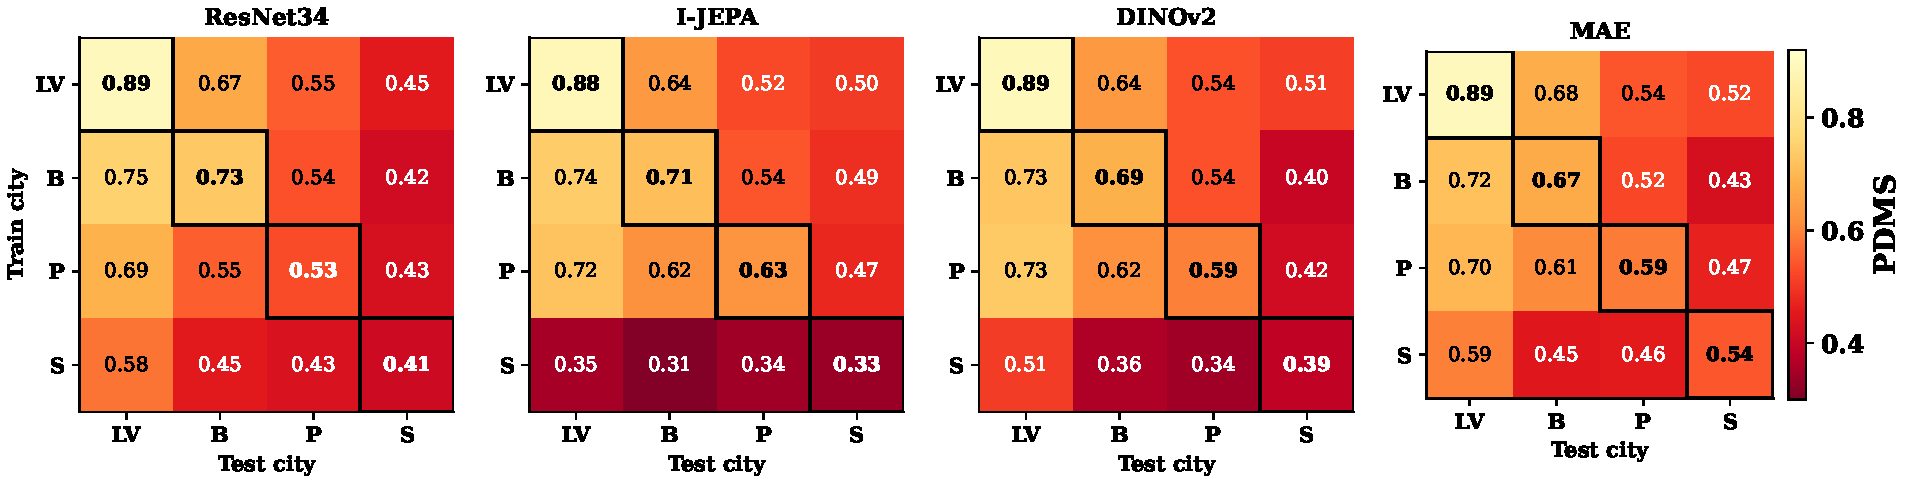
\includegraphics[width=0.48\textwidth]{iros/fig1_tf_pdms_heatmaps.pdf}
    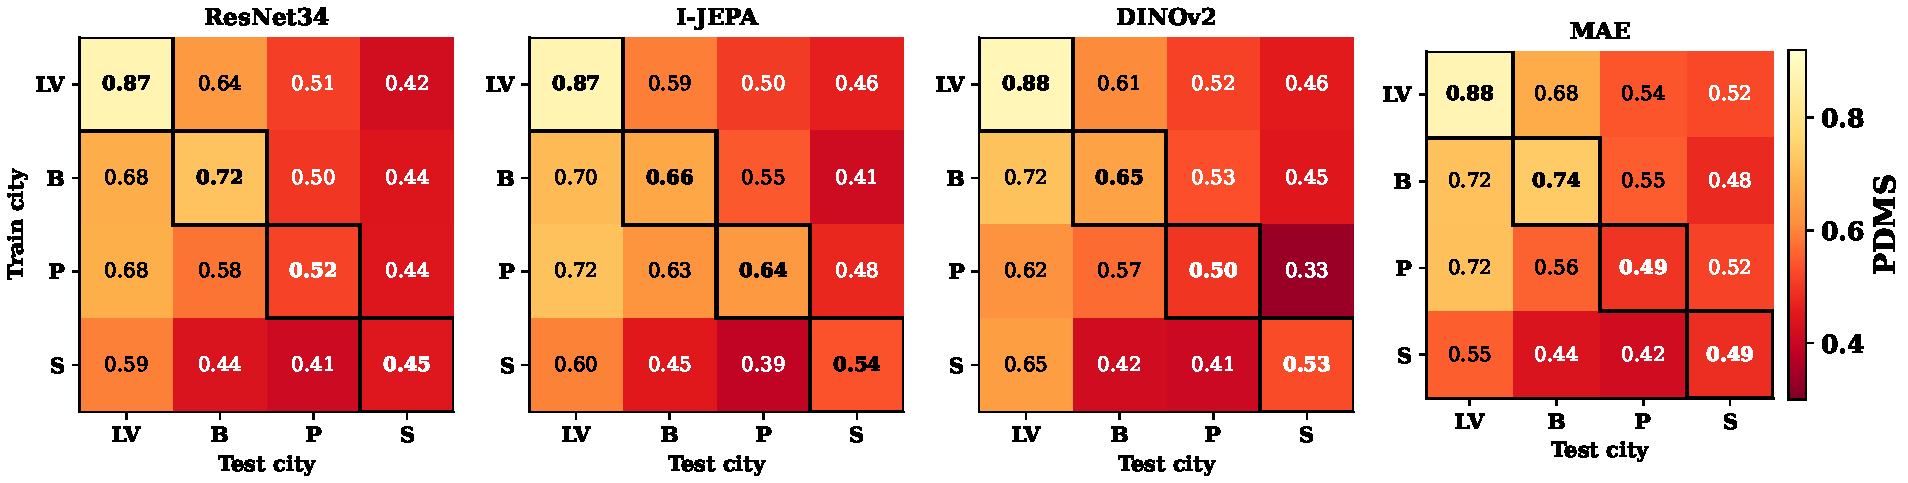
\includegraphics[width=0.48\textwidth]{iros/fig1_latf_pdms_heatmaps.pdf}
    \caption{Four-city cross-city PDMS matrices for TransFuser (left) and Latent TransFuser (right), pulled directly from our earlier cross-city benchmark study~\cite{naeinian-cross-city-2026}. Rows are training cities, columns are test cities, and each panel is a backbone family. The diagonal is in-distribution; off-diagonal cells expose the representation-dependent generalization gap. For every backbone, the Singapore column is the harshest; for supervised ResNet-34 (top-left panel), the off-diagonal penalty is larger and more uneven than for the frozen SSL panels.}
    \label{fig:iros-pdms-heatmaps}
\end{figure}

\subsection{OOD PDMS Analysis}
\label{sec:exp-phase1-ood}

The most direct open-loop evidence comes from transfer from Boston to Singapore on nuScenes. The supervised Swin backbone inflates from 0.60 to 5.86 average L2 and from 0.32 to 6.19 average collision rate, corresponding to 9.77$\times$ and 19.34$\times$ degradation. Replacing the backbone with a domain-specific SSL representation changes the picture entirely: the rectangular, frozen nuScenes-pretrained I-JEPA ViT-S/14 model yields an error ratio of only 1.20$\times$ in L2 and 0.75$\times$ in collision rate for the same transfer~\cite{naeinian-cross-city-2026}. The planning architecture is unchanged, so the improved robustness must come from the representation.

The closed-loop NAVSIM results point in the same direction. Generic large-scale SSL often matches or slightly exceeds the supervised ResNet34 baseline under single-city transfer, and domain-specific SSL is more reliable still. In the LiDAR-free Latent TransFuser setting, nuScenes-pretrained MAE improves average OOD PDMS by more than four points for Boston-, Pittsburgh-, and Las Vegas-trained models and by roughly three points for Singapore-trained models~\cite{naeinian-cross-city-2026}. The effect is therefore not a quirk of one backbone family or one planner: once city shift is explicit, self-supervised initialization systematically narrows the gap between in-domain and out-of-domain behavior.

\begin{figure}[ht]
    \centering
    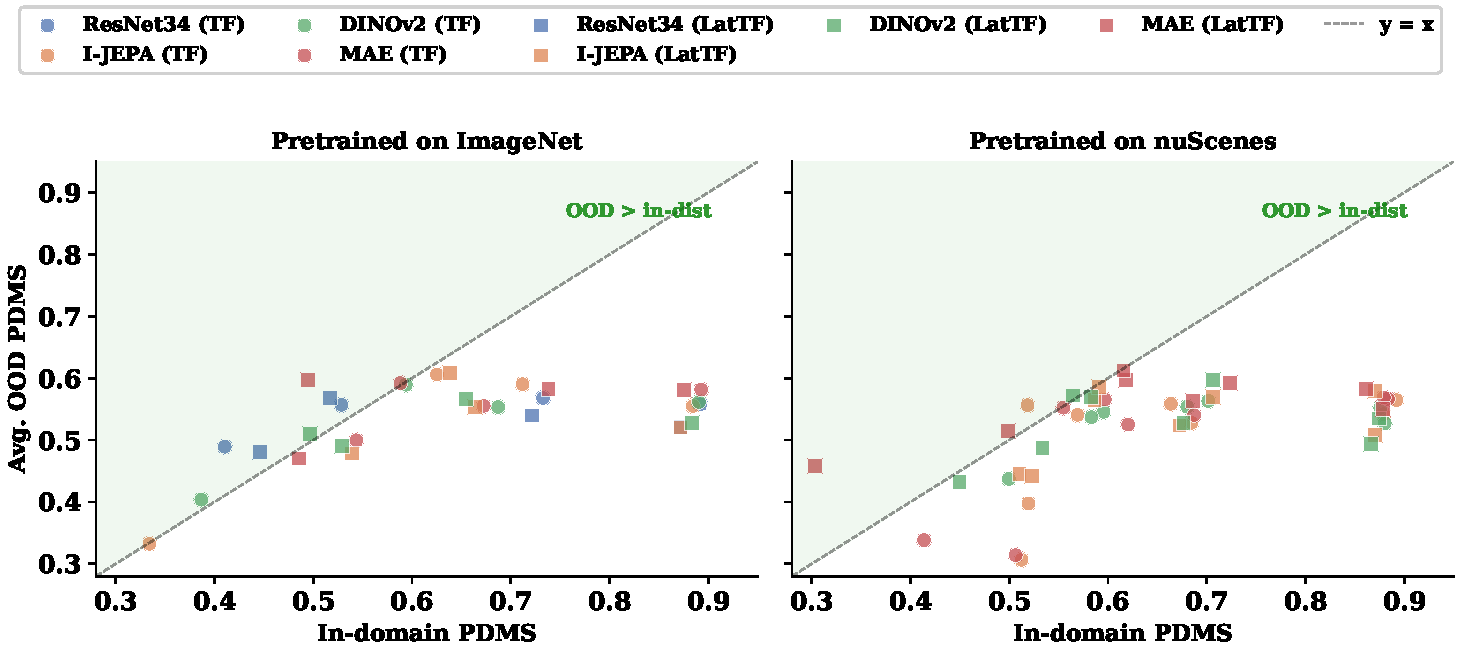
\includegraphics[width=0.75\textwidth]{iros/fig3_indomain_vs_ood.pdf}
    \caption{In-distribution PDMS versus average out-of-distribution PDMS across every cross-city configuration. Each point is one trained model; the diagonal is the reference ``no transfer penalty'' line. Points above the diagonal indicate in-distribution overfitting relative to OOD behavior. Supervised backbones (red) cluster further from the diagonal than frozen SSL backbones (blue) at every in-distribution score, consistent with the representation hypothesis. Source: Fig.~3 of our earlier cross-city benchmark study~\cite{naeinian-cross-city-2026}.}
    \label{fig:iros-indomain-vs-ood}
\end{figure}

Closed-loop cross-city transfer is further evaluated using the NAVSIM benchmark with the Performance Degradation Metric Score (PDMS), which measures driving task completion while penalizing infractions (higher is better). Table~\ref{tab:navsim_pdms_merged} reports PDMS across four cities --- Las Vegas (LV), Boston (B), Pittsburgh (P), and Singapore (S) --- for both TransFuser and Latent TransFuser under the NAVSIM v2.2 devkit; Table~\ref{tab:navsim_pdms_merged_v11} is the same matrix re-evaluated with the official NAVSIM v1.1 devkit as a defensive check against devkit-version confounders. For each backbone, we report results from all-city and single-city training to illustrate the impact of the geographic domain shift on closed-loop performance.

% Full NAVSIM v2.2 cross-city PDMS matrix (legacy devkit).
% Retained as provenance for the companion paper's numbers; the canonical
% thesis matrix is the v1.1 table (tab_navsim_pdms_merged_v11.tex).
\begin{sidewaystable}[p]
    \centering
    \caption[NAVSIM v2.2 cross-city PDMS matrix (legacy).]{%
    Full closed-loop cross-city PDMS matrix on NAVSIM, devkit v2.2 (legacy).
    Each row is a single trained model. The left block (\emph{Train City}) marks which of the four cities were used for training; \cmark indicates inclusion. Total combines performance across all four evaluation cities for each planner. All numbers are PDMS (\%); higher is better.
    How to read it: rows with four training cities are the all-city baselines, and their \emph{Total} column is mixed-city interpolation performance. Rows with a single training city are zero-shot transfer probes; non-checked columns under each planner are the out-of-distribution cells, and the gap between the in-distribution column and the three OOD columns quantifies the geographic transfer penalty. This matrix is retained for direct comparison with the companion cross-city benchmark paper~\cite{naeinian-cross-city-2026}; the thesis claims use the v1.1 re-evaluation in~\reftab{tab:navsim_pdms_merged_v11}.}
    \label{tab:navsim_pdms_merged}
    \scriptsize
    \setlength{\tabcolsep}{2pt}
    \renewcommand{\arraystretch}{0.95}
    \resizebox{\textwidth}{!}{%
    \begin{tabular}{|l|cccc|ccccc|ccccc|}
    \toprule
    \multirow{2}{*}{\textbf{Backbone}}
    & \multicolumn{4}{c|}{\textbf{Train City}}
    & \multicolumn{5}{c|}{\textbf{TransFuser (PDMS \%)}}
    & \multicolumn{5}{c|}{\textbf{Latent TransFuser (PDMS \%)}} \\
    \cmidrule(lr){2-5}\cmidrule(lr){6-10}\cmidrule(lr){11-15}
    & LV & B & P & S
    & LV & B & P & S & Total
    & LV & B & P & S & Total \\
    \midrule
    ResNet-34 supervised          & \cmark & \cmark & \cmark & \cmark & 88.4 & \textbf{81.4} & \textbf{75.7} & \textbf{59.9} & \textbf{79.2} & 87.0 & \textbf{79.3} & \textbf{74.4} & \textbf{67.2} & \textbf{79.0} \\
    ResNet-34 supervised          & --     & \cmark & --     & --     & 75.3 & 73.3 & 53.6 & 41.5 & 65.0 & 67.9 & 72.2 & 50.0 & 44.0 & 61.8 \\
    ResNet-34 supervised          & \cmark & --     & --     & --     & \textbf{89.2} & 67.0 & 55.1 & 45.3 & 68.6 & \textbf{87.2} & 63.6 & 50.9 & 41.9 & 65.5 \\
    ResNet-34 supervised          & --     & --     & \cmark & --     & 68.8 & 55.3 & 52.9 & 43.0 & 57.4 & 68.2 & 58.0 & 51.7 & 44.3 & 58.0 \\
    ResNet-34 supervised          & --     & --     & --     & \cmark & 57.9 & 45.5 & 43.4 & 41.0 & 48.5 & 59.3 & 43.9 & 41.1 & 44.6 & 48.6 \\
    \midrule
    I-JEPA ViT-H/14 frozen        & \cmark & \cmark & \cmark & \cmark & 86.5 & 77.1 & 71.2 & 68.1 & 77.6 & 85.0 & 76.5 & 69.6 & 68.7 & 76.7 \\
    I-JEPA ViT-H/14 100\% trainable & \cmark & \cmark & \cmark & \cmark & 87.4 & \textbf{77.7} & 68.8 & 64.2 & 77.0 & \textbf{89.3} & \textbf{77.8} & \textbf{73.0} & 67.6 & \textbf{79.1} \\
    I-JEPA ViT-S/14 nuSc rect., frozen        & \cmark & \cmark & \cmark & \cmark & 88.4 & 77.5 & \textbf{71.5} & 68.4 & \textbf{78.5} & 87.6 & 76.5 & 71.1 & 57.0 & 76.1 \\
    I-JEPA ViT-S/14 nuSc rect., trainable     & \cmark & \cmark & \cmark & \cmark & 88.9 & \textbf{77.7} & 70.8 & 67.0 & 78.4 & 86.6 & 74.8 & 67.2 & 65.3 & 75.7 \\
    I-JEPA ViT-S/14 nuSc sq., frozen          & \cmark & \cmark & \cmark & \cmark & 85.5 & 75.9 & 68.2 & \textbf{69.4} & 76.6 & 84.5 & 73.3 & 68.0 & 65.1 & 74.7 \\
    I-JEPA ViT-S/14 nuSc sq., trainable       & \cmark & \cmark & \cmark & \cmark & 86.7 & 76.2 & 70.9 & 65.7 & 77.0 & 82.9 & 69.8 & 59.1 & \textbf{70.2} & 72.1 \\
    I-JEPA ViT-H/14 frozen        & --     & \cmark & --     & --     & 74.1 & 71.2 & 54.2 & 48.8 & 65.2 & 70.2 & 66.4 & 54.7 & 41.2 & 61.3 \\
    I-JEPA ViT-H/14 trainable     & --     & \cmark & --     & --     & 72.5 & 68.0 & 52.4 & 40.9 & 62.1 & 71.7 & 68.5 & 55.0 & 47.8 & 63.6 \\
    I-JEPA ViT-H/14 frozen        & \cmark & --     & --     & --     & 88.4 & 63.6 & 52.5 & 50.5 & 67.6 & 87.2 & 59.2 & 50.5 & 46.4 & 64.8 \\
    I-JEPA ViT-H/14 trainable     & \cmark & --     & --     & --     & 88.3 & 62.2 & 52.9 & 50.1 & 67.1 & 83.1 & 62.0 & 52.5 & 44.7 & 64.4 \\
    I-JEPA ViT-H/14 frozen        & --     & --     & \cmark & --     & 72.1 & 62.2 & 62.5 & 47.4 & 63.3 & 72.0 & 62.9 & 63.9 & 47.5 & 63.7 \\
    I-JEPA ViT-H/14 trainable     & --     & --     & \cmark & --     & 70.1 & 60.4 & 60.1 & 37.4 & 60.0 & 64.0 & 60.1 & 55.8 & 33.8 & 56.4 \\
    I-JEPA ViT-H/14 frozen        & --     & --     & --     & \cmark & 35.1 & 30.5 & 34.1 & 33.4 & 33.2 & 59.6 & 45.1 & 38.8 & 53.9 & 50.1 \\
    I-JEPA ViT-H/14 trainable     & --     & --     & --     & \cmark & 58.1 & 44.9 & 43.8 & 48.8 & 49.7 & 64.0 & 44.9 & 41.3 & 50.8 & 51.5 \\
    \midrule
    DINOv2 ViT-S/14 frozen                    & \cmark & \cmark & \cmark & \cmark & 88.7 & 78.4 & 70.2 & 66.1 & 78.3 & 87.6 & 76.5 & 69.8 & 62.2 & 76.6 \\
    DINOv2 ViT-S/14 trainable                 & \cmark & \cmark & \cmark & \cmark & 86.0 & 74.4 & 66.0 & 68.9 & 75.7 & 86.4 & 72.1 & 63.2 & 56.0 & 72.5 \\
    DINOv2 ViT-S/14 nuSc rect., frozen        & \cmark & \cmark & \cmark & \cmark & 87.2 & 78.1 & 72.1 & 71.0 & 78.8 & 87.9 & 75.5 & 70.2 & 66.6 & 77.2 \\
    DINOv2 ViT-S/14 nuSc rect., trainable     & \cmark & \cmark & \cmark & \cmark & 88.5 & 79.7 & 74.1 & 67.9 & \textbf{79.7} & \textbf{88.3} & \textbf{79.8} & \textbf{73.1} & \textbf{71.3} & \textbf{79.9} \\
    DINOv2 ViT-S/14 nuSc sq., frozen          & \cmark & \cmark & \cmark & \cmark & 88.0 & \textbf{80.4} & \textbf{75.9} & 65.8 & \textbf{79.7} & 86.8 & 75.0 & 69.5 & 61.2 & 75.7 \\
    DINOv2 ViT-S/14 nuSc sq., trainable       & \cmark & \cmark & \cmark & \cmark & 87.7 & 77.1 & 68.4 & \textbf{71.5} & 78.0 & 83.7 & 73.0 & 64.2 & 66.7 & 73.8 \\
    \midrule
    MAE ViT-B/16 frozen                       & \cmark & \cmark & \cmark & \cmark & 89.5 & 80.9 & 75.1 & 65.5 & 80.2 & 87.6 & 76.9 & 70.5 & 69.5 & 78.0 \\
    MAE ViT-B/16 trainable                    & \cmark & \cmark & \cmark & \cmark & 86.3 & 78.6 & 69.3 & 67.8 & 77.6 & 86.3 & 76.5 & 68.5 & \textbf{74.9} & 77.9 \\
    MAE ViT-S/14 nuSc rect., frozen           & \cmark & \cmark & \cmark & \cmark & \textbf{90.3} & 80.2 & 74.2 & \textbf{73.7} & 81.4 & 85.3 & 77.3 & 72.9 & 69.9 & 77.9 \\
    MAE ViT-S/14 nuSc rect., trainable        & \cmark & \cmark & \cmark & \cmark & 89.9 & \textbf{82.4} & \textbf{77.4} & 72.6 & \textbf{82.4} & 89.2 & \textbf{79.9} & 70.2 & 68.9 & \textbf{79.3} \\
    MAE ViT-S/14 nuSc sq., frozen             & \cmark & \cmark & \cmark & \cmark & 88.9 & 78.6 & 73.7 & 68.3 & 79.4 & 84.5 & 75.2 & 71.5 & 67.3 & 76.3 \\
    MAE ViT-S/14 nuSc sq., trainable          & \cmark & \cmark & \cmark & \cmark & 87.4 & 77.8 & 74.2 & 70.6 & 79.2 & 85.8 & 77.7 & \textbf{74.4} & 64.1 & 77.6 \\
    \bottomrule
    \end{tabular}}%

    \vspace{0.6em}
    \footnotesize
    \emph{Single-city transfer rows for DINOv2 and MAE (Boston, Pittsburgh, Las~Vegas, Singapore) follow the same convention and are reported in the companion paper's supplementary material~\cite{naeinian-cross-city-2026}; the reduced set above is retained as the minimum provenance needed to justify the v1.1 re-evaluation used for all thesis claims.}
\end{sidewaystable}

% Full NAVSIM v1.1 cross-city PDMS matrix, canonical thesis table.
\begin{sidewaystable}[p]
    \centering
    \caption[NAVSIM v1.1 cross-city PDMS matrix (canonical).]{%
    Full closed-loop cross-city PDMS matrix on NAVSIM, devkit v1.1. This is the canonical closed-loop table used for every cross-city claim in the thesis. Each row is a single trained model; \emph{Train City} marks the cities used to fit that model. The two planner blocks (\emph{TransFuser}, \emph{Latent TransFuser}) report destination-city PDMS on the four NAVSIM test splits (LV, B, P, S) plus a \emph{Total} column averaging the four.
    How to read it: rows with all four training cities checked measure mixed-city interpolation; rows with a single training city measure zero-shot geographic transfer, in which case the three non-checked columns are the out-of-distribution cells. The gap between the in-distribution column and the OOD mean under a single planner isolates the transfer penalty; comparing the same row across the two planners separates backbone effects from head effects. All values are PDMS percentages; higher is better.}
    \label{tab:navsim_pdms_merged_v11}
    \scriptsize
    \setlength{\tabcolsep}{2pt}
    \renewcommand{\arraystretch}{0.95}
    \resizebox{\textwidth}{!}{%
    \begin{tabular}{|l|cccc|ccccc|ccccc|}
    \toprule
    \multirow{2}{*}{\textbf{Backbone}}
    & \multicolumn{4}{c|}{\textbf{Train City}}
    & \multicolumn{5}{c|}{\textbf{TransFuser (PDMS \%)}}
    & \multicolumn{5}{c|}{\textbf{Latent TransFuser (PDMS \%)}} \\
    \cmidrule(lr){2-5}\cmidrule(lr){6-10}\cmidrule(lr){11-15}
    & LV & B & P & S
    & LV & B & P & S & Total
    & LV & B & P & S & Total \\
    \midrule
    ResNet-34 supervised          & \cmark & \cmark & \cmark & \cmark & 86.6 & \textbf{78.4} & \textbf{73.8} & \textbf{64.0} & \textbf{77.9} & \textbf{89.0} & \textbf{82.5} & \textbf{80.3} & \textbf{66.5} & \textbf{81.7} \\
    ResNet-34 supervised          & --     & \cmark & --     & --     & 75.3 & 73.3 & 53.6 & 41.5 & 65.0 & 67.3 & 71.7 & 54.5 & 45.0 & 62.6 \\
    ResNet-34 supervised          & \cmark & --     & --     & --     & \textbf{89.2} & 67.0 & 55.1 & 45.3 & 68.6 & 86.9 & 62.1 & 53.2 & 42.3 & 65.5 \\
    ResNet-34 supervised          & --     & --     & \cmark & --     & 68.8 & 55.3 & 52.9 & 43.0 & 57.4 & 67.7 & 57.5 & 53.0 & 46.5 & 58.3 \\
    ResNet-34 supervised          & --     & --     & --     & \cmark & 56.6 & 45.4 & 49.6 & 42.1 & 49.5 & 57.4 & 42.6 & 45.1 & 45.5 & 48.5 \\
    \midrule
    I-JEPA ViT-H/14 frozen        & \cmark & \cmark & \cmark & \cmark & 85.3 & 75.7 & 72.4 & 67.3 & 76.9 & 83.7 & 75.2 & 70.9 & \textbf{68.3} & 76.1 \\
    I-JEPA ViT-H/14 trainable     & \cmark & \cmark & \cmark & \cmark & 86.6 & \textbf{77.1} & 70.6 & 64.8 & 77.0 & \textbf{88.7} & \textbf{77.3} & 75.1 & 67.1 & \textbf{79.1} \\
    I-JEPA ViT-S/14 nuSc rect., frozen        & \cmark & \cmark & \cmark & \cmark & 87.3 & 77.0 & \textbf{74.3} & \textbf{69.2} & \textbf{78.7} & 86.6 & 73.3 & 69.7 & 59.9 & 74.9 \\
    I-JEPA ViT-S/14 nuSc rect., trainable     & \cmark & \cmark & \cmark & \cmark & 89.0 & 76.8 & 73.3 & 67.0 & 78.6 & 86.2 & 73.9 & 74.7 & 59.5 & 75.9 \\
    I-JEPA ViT-S/14 nuSc sq., frozen          & \cmark & \cmark & \cmark & \cmark & 84.8 & 75.1 & 69.7 & 69.1 & 76.3 & 83.8 & 73.2 & 68.6 & 61.5 & 74.0 \\
    I-JEPA ViT-S/14 nuSc sq., trainable       & \cmark & \cmark & \cmark & \cmark & 85.8 & 75.7 & 73.0 & 65.2 & 76.9 & 87.3 & 76.4 & \textbf{75.3} & 67.7 & 78.5 \\
    I-JEPA ViT-H/14 frozen        & --     & \cmark & --     & --     & 72.5 & 69.9 & 58.2 & 50.1 & 65.3 & 69.4 & 67.5 & 62.2 & 42.2 & 63.1 \\
    I-JEPA ViT-H/14 trainable     & --     & \cmark & --     & --     & 72.0 & 68.9 & 60.1 & 42.0 & 63.9 & 70.7 & 68.2 & 60.7 & 48.7 & 64.5 \\
    I-JEPA ViT-H/14 frozen        & \cmark & --     & --     & --     & 86.9 & 61.2 & 53.7 & 51.4 & 66.7 & 85.9 & 57.5 & 51.9 & 47.8 & 64.3 \\
    I-JEPA ViT-H/14 trainable     & \cmark & --     & --     & --     & 87.7 & 60.1 & 53.9 & 51.3 & 66.7 & 82.7 & 60.3 & 54.8 & 44.3 & 64.2 \\
    I-JEPA ViT-H/14 frozen        & --     & --     & \cmark & --     & 71.4 & 61.3 & 64.5 & 49.5 & 63.5 & 71.8 & 63.5 & 69.0 & 48.6 & 65.0 \\
    I-JEPA ViT-H/14 trainable     & --     & --     & \cmark & --     & 69.1 & 59.6 & 65.3 & 39.0 & 60.7 & 63.7 & 60.1 & 59.4 & 35.4 & 57.3 \\
    I-JEPA ViT-H/14 frozen        & --     & --     & --     & \cmark & 36.0 & 35.9 & 45.1 & 35.6 & 37.7 & 58.3 & 44.6 & 43.0 & 55.6 & 50.6 \\
    I-JEPA ViT-H/14 trainable     & --     & --     & --     & \cmark & 56.7 & 45.3 & 48.0 & 50.3 & 50.4 & 62.7 & 43.9 & 44.4 & 52.8 & 51.7 \\
    \midrule
    DINOv2 ViT-S/14 frozen                    & \cmark & \cmark & \cmark & \cmark & 87.7 & 77.0 & 71.5 & 66.0 & 77.7 & 86.4 & 72.8 & 67.2 & 59.2 & 74.1 \\
    DINOv2 ViT-S/14 trainable                 & \cmark & \cmark & \cmark & \cmark & 85.4 & 73.5 & 67.6 & 68.9 & 75.6 & 82.7 & 68.9 & 64.0 & 54.2 & 70.2 \\
    DINOv2 ViT-S/14 nuSc rect., frozen        & \cmark & \cmark & \cmark & \cmark & 86.6 & 77.2 & 74.0 & 70.5 & 78.7 & 87.1 & 74.8 & 71.6 & \textbf{71.5} & 77.7 \\
    DINOv2 ViT-S/14 nuSc rect., trainable     & \cmark & \cmark & \cmark & \cmark & 87.9 & 79.0 & 76.2 & 67.4 & \textbf{79.6} & 87.3 & \textbf{78.5} & \textbf{75.7} & 66.7 & \textbf{79.0} \\
    DINOv2 ViT-S/14 nuSc sq., frozen          & \cmark & \cmark & \cmark & \cmark & 87.2 & \textbf{79.2} & \textbf{77.8} & 65.5 & 79.4 & 86.3 & 73.1 & 72.7 & 60.8 & 75.5 \\
    DINOv2 ViT-S/14 nuSc sq., trainable       & \cmark & \cmark & \cmark & \cmark & 86.3 & 75.9 & 69.0 & \textbf{71.2} & 77.3 & 86.7 & 73.6 & 70.6 & 71.2 & 77.0 \\
    \midrule
    MAE ViT-B/16 frozen                       & \cmark & \cmark & \cmark & \cmark & 89.0 & 80.8 & \textbf{78.7} & 65.1 & 80.7 & 81.7 & 70.7 & 62.8 & 69.9 & 72.7 \\
    MAE ViT-B/16 trainable                    & \cmark & \cmark & \cmark & \cmark & 85.4 & 78.0 & 73.9 & 67.4 & 78.0 & 88.7 & \textbf{81.9} & \textbf{80.0} & 61.6 & 80.6 \\
    MAE ViT-S/14 nuSc rect., frozen           & \cmark & \cmark & \cmark & \cmark & 89.2 & 79.1 & 75.1 & \textbf{73.1} & 80.7 & 87.4 & 79.2 & 79.8 & 64.6 & 79.8 \\
    MAE ViT-S/14 nuSc rect., trainable        & \cmark & \cmark & \cmark & \cmark & 89.3 & \textbf{81.2} & 78.4 & 72.1 & \textbf{81.9} & 86.2 & 79.7 & 77.8 & 72.3 & 80.3 \\
    MAE ViT-S/14 nuSc sq., frozen             & \cmark & \cmark & \cmark & \cmark & 87.7 & 77.3 & 75.2 & 67.8 & 78.9 & 86.4 & 75.0 & 70.3 & 67.9 & 76.7 \\
    MAE ViT-S/14 nuSc sq., trainable          & \cmark & \cmark & \cmark & \cmark & 86.9 & 77.3 & 76.3 & 70.3 & 79.2 & \textbf{89.3} & 78.5 & 78.0 & \textbf{74.1} & \textbf{81.4} \\
    MAE ViT-B/16 frozen                       & --     & \cmark & --     & --     & 70.6 & 67.0 & 56.8 & 43.4 & 62.4 & 71.8 & 73.4 & 60.0 & 48.7 & 66.3 \\
    MAE ViT-B/16 trainable                    & --     & \cmark & --     & --     & 70.6 & 67.3 & 58.0 & 41.9 & 62.5 & 69.4 & 73.1 & 61.3 & 53.7 & 66.5 \\
    MAE ViT-B/16 frozen                       & \cmark & --     & --     & --     & 88.3 & 66.2 & 55.2 & 52.9 & 69.3 & 86.6 & 66.0 & 56.1 & 52.2 & 68.8 \\
    MAE ViT-B/16 trainable                    & \cmark & --     & --     & --     & 87.4 & 59.8 & 53.2 & 51.6 & 66.4 & 87.8 & 63.3 & 56.0 & 51.0 & 68.1 \\
    MAE ViT-B/16 frozen                       & --     & --     & \cmark & --     & 69.3 & 59.9 & 61.1 & 48.9 & 61.5 & 71.2 & 54.8 & 50.4 & 52.6 & 59.1 \\
    MAE ViT-B/16 trainable                    & --     & --     & \cmark & --     & 73.0 & 65.6 & 68.8 & 40.8 & 64.8 & 64.4 & 63.9 & 61.0 & 35.7 & 59.1 \\
    MAE ViT-B/16 frozen                       & --     & --     & --     & \cmark & 58.0 & 45.3 & 51.2 & 56.7 & 52.5 & 54.6 & 44.0 & 46.6 & 49.7 & 49.0 \\
    MAE ViT-B/16 trainable                    & --     & --     & --     & \cmark & 51.0 & 46.0 & 52.2 & 36.0 & 47.3 & 55.6 & 43.8 & 48.0 & 42.5 & 48.4 \\
    \bottomrule
    \end{tabular}}
\end{sidewaystable}

\begin{table}[ht]
\centering
\caption[Boston-only v1.1 Latent TransFuser cross-city summary.]{%
Compact summary of the canonical Boston-trained Latent TransFuser rows from the v1.1 matrix in~\reftab{tab:navsim_pdms_merged_v11}. These four rows are used as the matched supervised-vs-SSL comparison throughout the thesis: each model is trained on Boston only and evaluated on every NAVSIM city. LV/B/P/S are destination-city PDMS percentages; the in-distribution column (bold) is Boston; \emph{OOD mean} averages the three remaining cities and \emph{Drop} is the in-distribution-minus-OOD-mean gap in percentage points. A smaller drop indicates a more geographically robust representation under a fixed planner. The MAE row has the best absolute OOD mean; the DINOv2 row has the smallest drop; the ResNet-34 row has the largest drop and is the supervised reference.}
\label{tab:navsim_pdms_boston_v11}
\vspace{0.35em}
\small
\renewcommand{\arraystretch}{1.15}
\setlength{\tabcolsep}{5pt}
\begin{tabular}{@{}>{\raggedright\arraybackslash}p{3.6cm} c c c c c c@{}}
\toprule
\textbf{Backbone} & \textbf{LV (\%)} & \textbf{B (\%)} & \textbf{P (\%)} & \textbf{S (\%)} & \textbf{OOD mean (\%)} & \textbf{Drop (pp)} \\
\midrule
\rowcolor{gray!12}
ResNet-34 supervised & 67.3 & \textbf{71.7} & 54.5 & 45.0 & 55.6 & \textbf{16.1} \\
MAE ViT-B/16 frozen  & 71.8 & \textbf{73.4} & 60.0 & 48.7 & \textbf{60.2} & 13.2 \\
I-JEPA ViT-H/14 frozen & 69.4 & \textbf{67.5} & 62.2 & 42.2 & 57.9 & 9.6 \\
DINOv2 ViT-S/14 frozen & 70.7 & \textbf{63.6} & 55.8 & 45.5 & 57.3 & \textbf{6.3} \\
\bottomrule
\end{tabular}
\end{table}

\FloatBarrier

\subsection{Best Training Ground (RQ2)}
\label{sec:exp-phase1-best-training-city}

Which source city gives the most transferable planner? \reffig{fig:iros-best-training-city} aggregates this across all backbones and heads. Las Vegas and Boston alternate as the top two; Pittsburgh is consistently mid-tier; Singapore is the worst single-city training source in every configuration, for the reasons discussed in the data card (\refapp{app:city-data-card}). The same pattern appears more compactly in the radar plot (\reffig{fig:iros-radar}), which shows per-city in-distribution and OOD PDMS for each of the strongest backbones. The radar reveals a useful operational criterion: the best single-city training source is the one whose in-distribution contour most nearly matches its OOD contour, i.e.\ whose model maintains similar competence under transfer rather than simply being strongest on its own city.

\begin{figure}[ht]
    \centering
    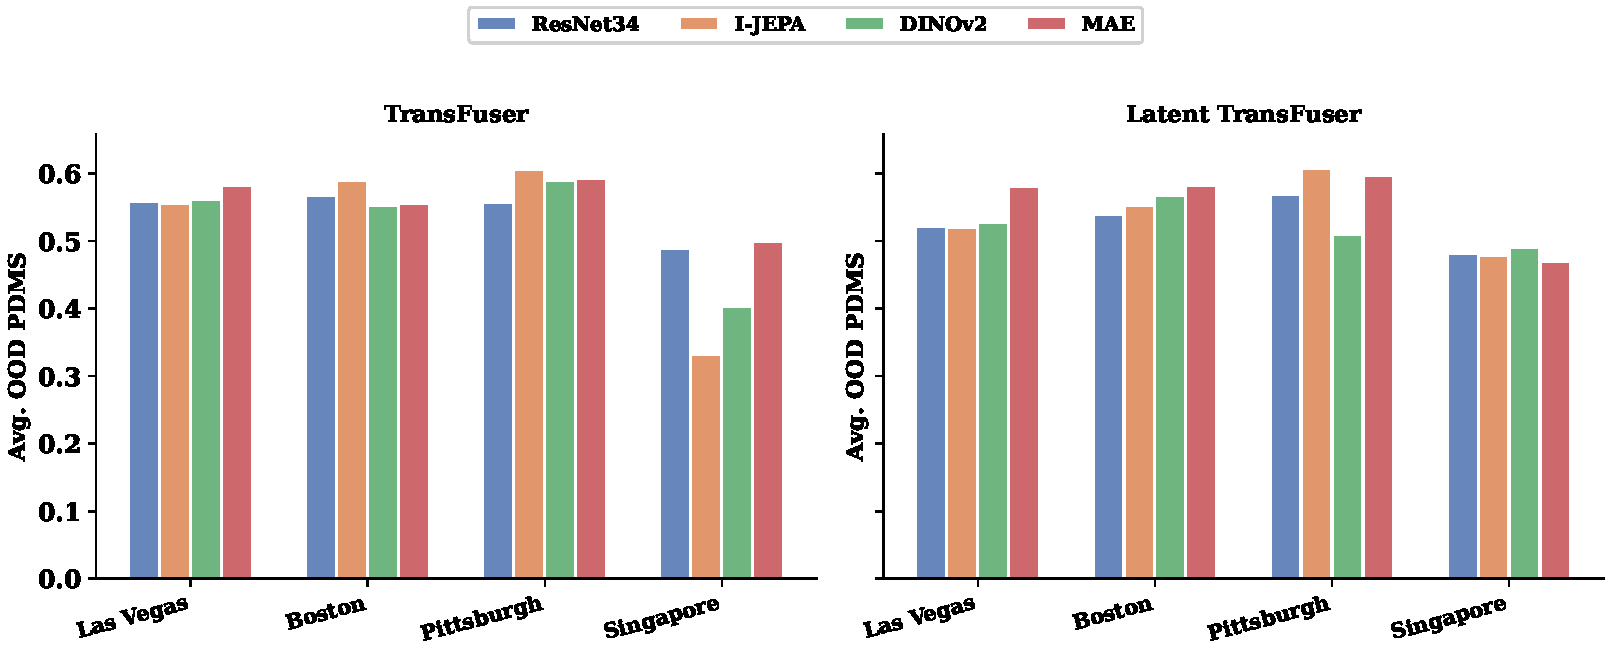
\includegraphics[width=0.75\textwidth]{iros/fig6_best_training_city.pdf}
    \caption{Average cross-city PDMS achieved by each of the four single-city training sources, grouped by backbone family. The ranking Las Vegas $\geq$ Boston $>$ Pittsburgh $>$ Singapore is stable across backbones; the absolute spread is larger for supervised ResNet-34 than for frozen SSL variants, consistent with the representation-centric account. Source: Fig.~6 of~\cite{naeinian-cross-city-2026}.}
    \label{fig:iros-best-training-city}
\end{figure}

\begin{figure}[ht]
    \centering
    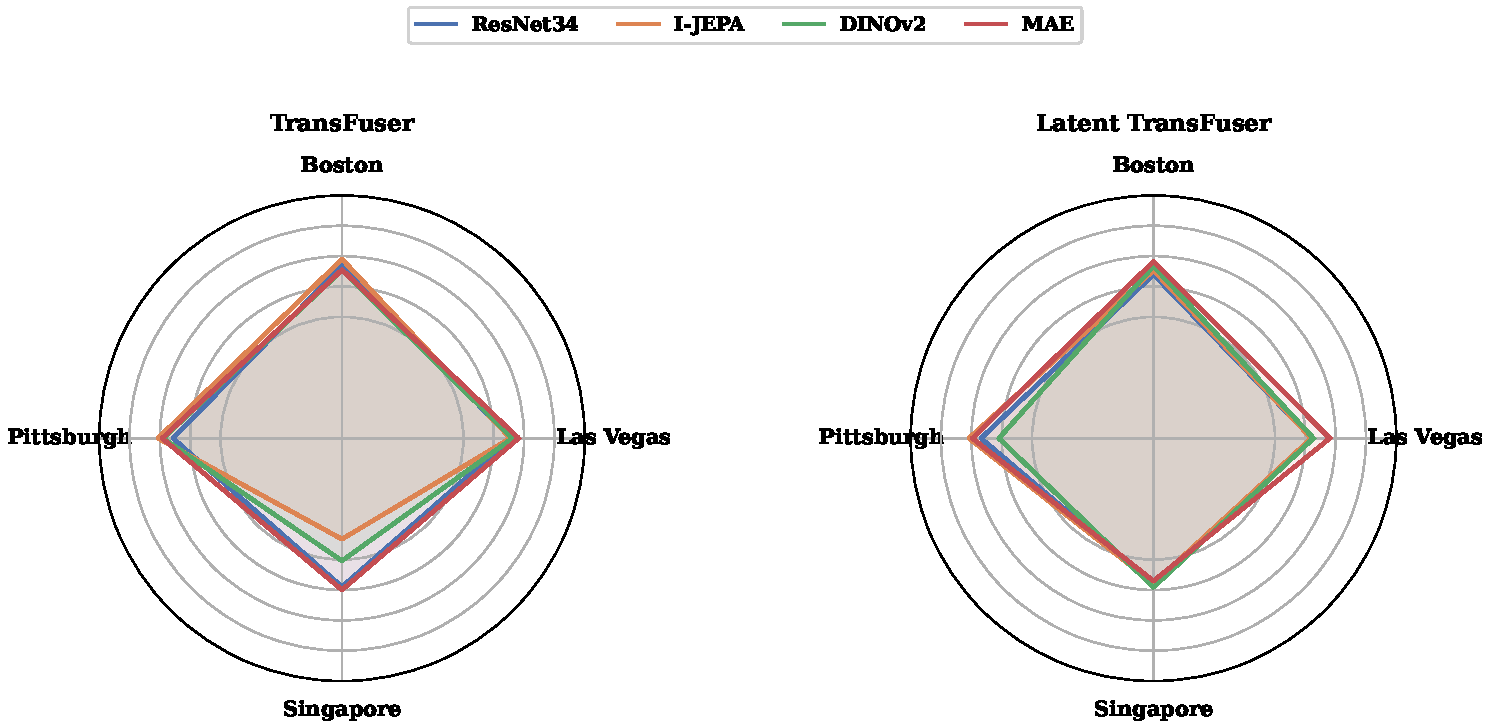
\includegraphics[width=0.9\textwidth]{iros/fig12_radar_summary.pdf}
    \caption{Radar summary of per-city PDMS by training source (rows) and backbone family (panels). The filled area is the average of the four per-city scores; wider, rounder areas correspond to more uniform transfer. Frozen SSL radars are more nearly circular than supervised ResNet radars, which is a compact visual restatement of the order-of-magnitude robustness claim. Source: Fig.~12 of~\cite{naeinian-cross-city-2026}.}
    \label{fig:iros-radar}
\end{figure}

\subsection{Transfer Asymmetry Analysis}
\label{sec:exp-phase1-asymmetry}

Transfer asymmetry is not noise; it is one of the most important findings of the benchmark. The hardest direction is typically from a right-hand-traffic city into Singapore, not the reverse. That asymmetry is consistent with a representational explanation: a backbone trained only on right-hand-traffic scenes can overfit to layout priors that become actively misleading in Singapore, whereas a model trained in Singapore is forced to encode some structure that remains useful when moved back to right-hand-traffic cities. Dataset scale compounds the effect. Singapore is also the smallest source domain in NAVSIM, so a model trained there has fewer opportunities to learn a diverse but reusable representation~\cite{naeinian-cross-city-2026}.

\begin{figure}[ht]
    \centering
    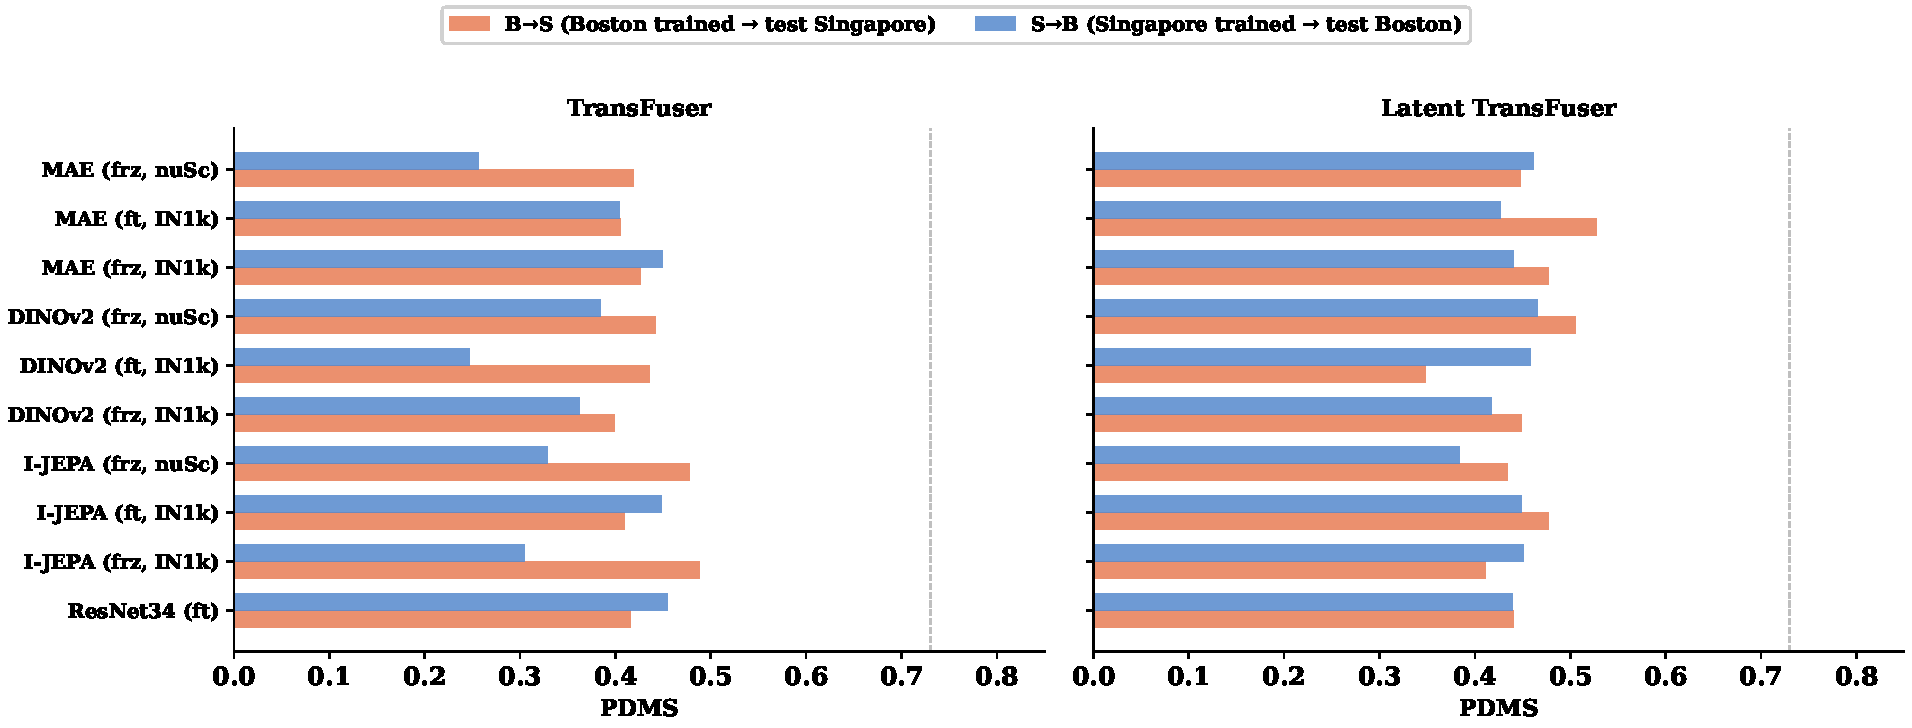
\includegraphics[width=0.7\textwidth]{iros/fig8_asymmetry.pdf}
    \caption[Boston--Singapore transfer asymmetry (bar chart).]{Boston$\leftrightarrow$Singapore transfer asymmetry. Bars are OOD PDMS at the destination; the grouped comparison isolates the direction of transfer. Boston$\rightarrow$Singapore is the harsher direction for every backbone, consistent with the dataset-scale and traffic-convention asymmetry discussed in-text. The absolute asymmetry gap is smaller for frozen SSL than for supervised ResNet-34. Source: Fig.~8 of~\cite{naeinian-cross-city-2026}.}
    \label{fig:iros-asymmetry}
\end{figure}

\subsection{Per-Metric Breakdown}
\label{sec:exp-phase1-metrics}

The phase-1 preprint primarily reports aggregate PDMS rather than a full decomposition into the five PDMS components for every transfer pair. For that reason, the thesis uses total PDMS as the main closed-loop robustness indicator in this chapter. The important point is that the gap is visible at the level of overall driving competence before any sub-score decomposition is introduced: geographic shift degrades planning quality substantially, and the degradation is consistently smaller when the backbone is self-supervised.

\begin{figure}[ht]
    \centering
    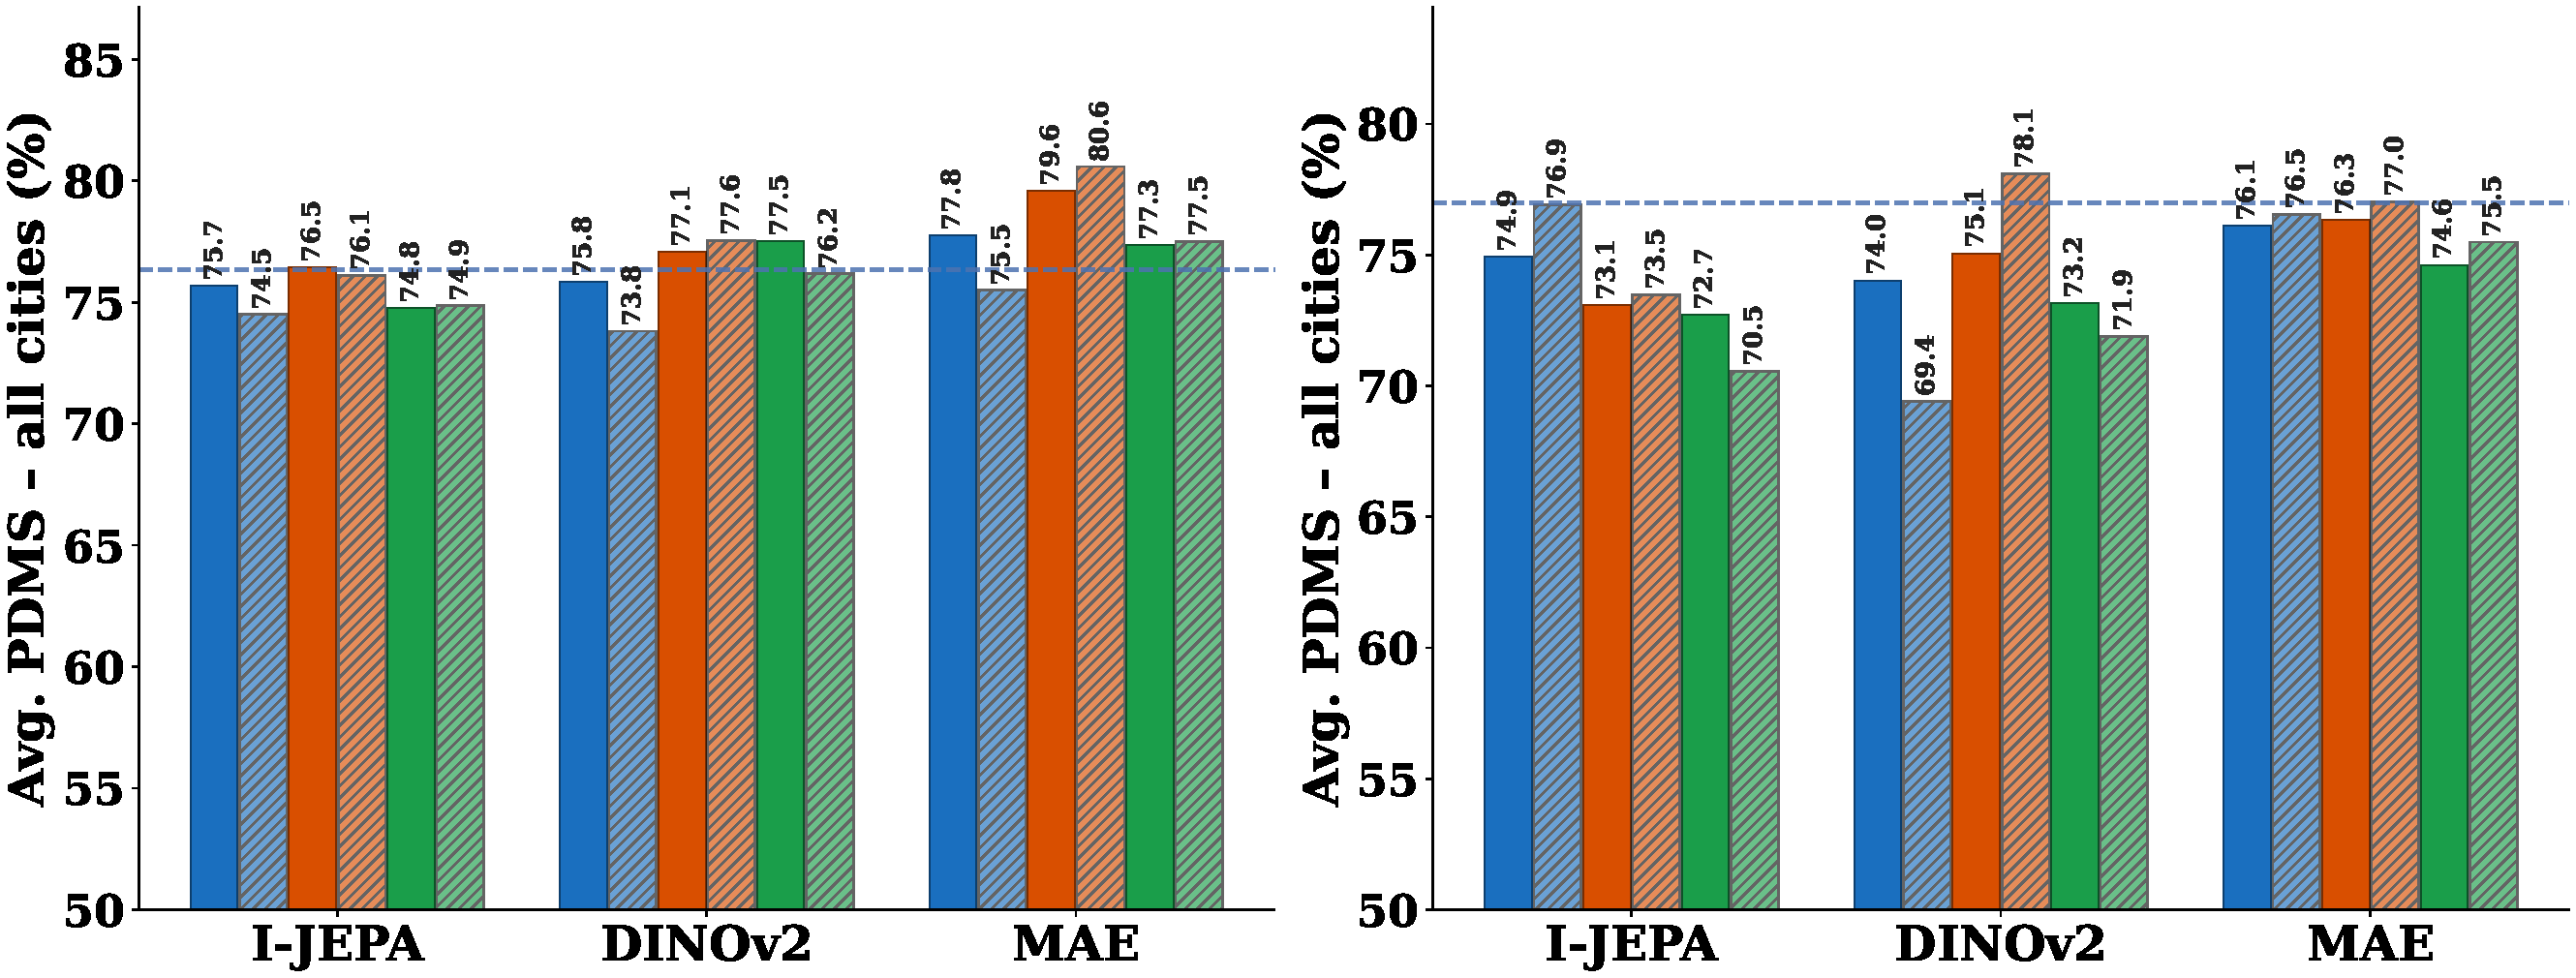
\includegraphics[width=0.85\textwidth]{iros/fig14_allcity_training.pdf}
    \caption{All-city training comparison. Mixed-city NAVSIM training pools examples from every city, which narrows the gap between supervised and SSL backbones as the dataset becomes geographically diverse. The takeaway is not that supervised backbones are equivalent to SSL --- they remain behind on the transfer matrices --- but that any benchmark that only reports mixed-city PDMS is measuring a regime in which the representation question is effectively washed out. Source: Fig.~14 of~\cite{naeinian-cross-city-2026}.}
    \label{fig:iros-allcity}
\end{figure}

% ============================================================================
\section{SSL Backbones in Generative Planning}
\label{sec:exp-phase2}

The generative-planning study revisits in-distribution NAVSIM under a planner that is designed to attenuate backbone contributions: DiffusionDrive~\cite{jia-diffusiondrive-2025}. Chapter~\ref{chap:methodology}, Section~\ref{sec:meth-dd-why} develops the rationale in full; the short form is that DiffusionDrive denoises trajectories from K-means anchor initializations in two steps, conditions through grid-sampled BEV cross-attention, and uses time-only FiLM, and the composite effect is a head that can produce good trajectories even when the image features are weak. This makes DiffusionDrive a deliberately hostile substrate for the representation claim. The goal of this study is therefore not to top an in-distribution leaderboard; it is to measure whether any backbone-dependent structure survives DiffusionDrive's attenuation, because that is the harder precondition for the cross-city generative study in \refsec{sec:exp-phase3}. The ViT adapter is held identical to the one used in the cross-city benchmark (both pipelines import \texttt{create\_image\_encoder} from the same TransFuser backbone module), so the planner head is the only manipulated variable between the two studies.

\begin{table}[ht]
\centering
\caption{DiffusionDrive + SSL backbone results on NAVSIM (all cities).}
\label{tab:diffusiondrive-allcity}
\begin{tabular}{lllcc}
\toprule
\textbf{Exp} & \textbf{Backbone} & \textbf{Modality} & \textbf{Frozen} & \textbf{PDMS} \\
\midrule
A12   & ResNet34              & C+L & ---       & 87.9 \\
A12-o & MAE (rect, trainable) & C+L & No        & 86.9 \\
A12-u & MAE (sq, trainable)   & C+L & No        & 86.8 \\
A12-q & I-JEPA (sq, trainable)& C+L & No        & 86.2 \\
A10-j & I-JEPA nuSc (rect, frozen) & C+L & Yes  & 85.2 \\
A10-p & I-JEPA nuSc (sq, frozen)   & C+L & Yes  & 86.3 \\
A13   & ResNet34 (camera-only)& C   & ---       & 86.6 \\
\bottomrule
\end{tabular}
\end{table}

\subsection{SSL vs.\ Supervised in Generative Planning}
\label{sec:exp-phase2-ssl-vs-sup}

The $\sim$1pp gap between SSL (86.2--86.9) and supervised ResNet34 (87.9) on all-city training mirrors the pattern from the cross-city benchmark. SSL features are slightly weaker in-distribution in this architecture as well. That observation is important in the context of the broader thesis: if mixed-city PDMS were the only question, stronger planner design could easily dominate the narrative. Instead, the small in-distribution cost becomes interesting only because later studies ask whether SSL repays that cost under domain shift.

\subsection{Camera-Only: SSL Partially Replaces LiDAR}
\label{sec:exp-phase2-camera-only}

The camera-only baseline is already stronger than one might expect. ResNet34 camera-only (A13) reaches 86.6 PDMS, only 1.3 points below the corresponding camera+LiDAR configuration at 87.9. This narrows the remaining question: the issue is no longer whether camera-only planning is viable at all, but whether stronger visual pretraining can close the residual gap without reintroducing expensive sensors. The planned I-JEPA camera-only experiment is therefore not a side experiment; it is the most direct test of whether SSL features can substitute for part of the geometric information usually supplied by LiDAR.

\paragraph{Planned I-JEPA camera-only comparison (designed, pending).}
Starting from the A13 ResNet-34 camera-only baseline ($86.6$ PDMS, \reftab{tab:diffusiondrive-allcity}), the supervised encoder is replaced with the strongest frozen SSL variant: I-JEPA ViT-S/14 nuScenes square, frozen (A10-p, $86.3$ PDMS in a camera+LiDAR configuration). Configuration is in \reftab{tab:exp-camonly-config}; pre-registered reading bands are in \reftab{tab:exp-camonly-bands}.

\begin{table}[ht]
\centering
\caption{Configuration for the planned I-JEPA camera-only comparison. All fields are held fixed to the A10-p / A13 hyperparameters; only the backbone and the LiDAR modality differ from their respective cells of \reftab{tab:diffusiondrive-allcity}.}
\label{tab:exp-camonly-config}
\small
\setlength{\tabcolsep}{6pt}
\renewcommand{\arraystretch}{1.15}
\begin{tabular}{@{}>{\raggedright\arraybackslash}p{3.6cm} >{\raggedright\arraybackslash}p{8.4cm}@{}}
\toprule
\textbf{Setting} & \textbf{Value} \\
\midrule
Backbone        & I-JEPA ViT-S/14, nuScenes square pre-training, frozen \\
Modality        & Camera only (LiDAR removed) \\
Optimizer       & Adam, constant LR $1\times10^{-4}$ \\
Epochs          & $20$ \\
Anchor bank     & $256$ K-means trajectories on \texttt{navtrain} \\
Denoising steps & $2$ (truncated) at inference \\
Training split  & \texttt{navtrain}, all cities \\
Reference rows  & A10-p ($86.3$ PDMS, C+L), A13 ($86.6$ PDMS, camera-only) \\
\bottomrule
\end{tabular}
\end{table}

\begin{table}[ht]
\centering
\caption{Pre-registered reading of the planned camera-only PDMS outcome. Bands are fixed before the run; interpretation follows directly.}
\label{tab:exp-camonly-bands}
\small
\setlength{\tabcolsep}{6pt}
\renewcommand{\arraystretch}{1.2}
\begin{tabular}{@{}>{\raggedright\arraybackslash}p{2.5cm} >{\raggedright\arraybackslash}p{2.9cm} >{\raggedright\arraybackslash}p{6.6cm}@{}}
\toprule
\textbf{Band} & \textbf{PDMS range} & \textbf{Interpretation} \\
\midrule
Full compensation & $\geq 86.6$            & Representation fully replaces LiDAR \\
Partial           & $85.5$--$86.5$         & Modest gain over supervised camera-only at no LiDAR cost \\
Null              & $< 85.0$               & Frozen SSL does not recover the LiDAR contribution at this scale \\
\bottomrule
\end{tabular}
\end{table}

\subsection{Frozen vs.\ Fine-Tuned Backbone}
\label{sec:exp-phase2-frozen}

Within DiffusionDrive, the I-JEPA results show that preprocessing matters at least as much as fine-tuning. The rectangular frozen run reaches 85.2 PDMS, the square-crop frozen run reaches 86.3, and the trainable square-crop run reaches 86.2. The simplest interpretation is that matching the pretraining geometry of the ViT is more important than unfreezing the backbone, at least on the mixed-city split. This fits the broader thesis argument that frozen SSL weights act as a form of implicit regularization: they preserve the pretrained invariances while still allowing the adapter and planner to specialize downstream.

% ============================================================================
\section{Cross-City Generative Planning Protocol (Designed; Pending)}
\label{sec:exp-phase3}

The cross-city generative study extends the representation-centric cross-city benchmark into the generative-planning regime. The protocol is already defined and the training pipeline is ready to launch; the experimental runs themselves are scheduled outside the window of this thesis and will be reported in a follow-up publication. We document the protocol here with the same level of detail as the completed studies so that the design can be scrutinized (and replicated) independently of its execution.

\subsection{Rationale}
\label{sec:exp-phase3-rationale}

Two observations from the preceding studies motivate the cross-city generative study. First, Drive-JEPA~\cite{wang-drive-jepa} showed that mixed-city NAVSIM is no longer informative about a backbone's cross-city invariance --- a sufficiently strong generative planner closes the in-distribution gap regardless of backbone, which is precisely the effect our generative-planning results replicate for DiffusionDrive. Second, our earlier cross-city benchmark~\cite{naeinian-cross-city-2026} showed that geographic shift is the regime in which representation choice becomes load-bearing for the lightweight LAW and TransFuser heads.

The cross-city generative study asks whether that second observation survives the substitution of a generative planner for a regression one \emph{where the generative planner is hostile to the backbone by construction}. The reading criterion, set in advance and developed in \refsec{sec:meth-dd-success}, is directional: frozen SSL is required to produce a smaller OOD PDMS drop than supervised ResNet-34 in three or more of the four training-city rows for the representation-centric claim to be judged architecture-agnostic. Because DiffusionDrive's K-means anchor initialization, two-step denoising, and grid-sampled BEV conditioning attenuate the backbone's contribution, small absolute PDMS differences at the ratio level (in-distribution over OOD) are the load-bearing quantity; the thesis reports transfer-ratio inflation rather than raw PDMS gaps for this study.

\subsection{Experimental Matrix}
\label{sec:exp-phase3-matrix}

Two backbones $\times$ four training cities = eight training runs; each run is then evaluated on all four city test sets, for 32 closed-loop evaluations total. The backbones are chosen to pair a supervised baseline with the best generative-planning SSL configuration:
\begin{itemize}
    \item \textbf{ResNet-34 (C+L)} --- the all-city A12 configuration (87.9 PDMS, Table~\ref{tab:diffusiondrive-allcity}). Trainable, following the DiffusionDrive recipe.
    \item \textbf{I-JEPA ViT-S/14 nuScenes sq.\ frozen (C+L)} --- the A10-p configuration (86.3 PDMS), selected because (a) its square-crop geometry matches the ViT pretraining, (b) frozen SSL is the operational lever that matters for transfer per \refsec{sec:exp-why-ssl}, and (c) it is the strongest frozen DiffusionDrive configuration we measured in the generative-planning study.
\end{itemize}

Except for the training-city filter, every other hyperparameter (optimizer, learning rate, epoch count, batch size, anchor bank, denoising steps) is inherited from the generative-planning study's all-city configuration so that the cross-city generative study isolates the effect of geographic shift.

% Legacy protocol sketch retained for provenance. The completed matrix is in experiments.tex.
\begin{table}[ht]
    \centering
    \caption[Legacy cross-city generative study protocol sketch.]{Legacy protocol sketch for the initial two-backbone cross-city generative plan. The completed DiffusionDrive matrix reported in Chapter~\ref{chap:experiments} supersedes this table.}
    \label{tab:phase3-plan}
    \small
    \setlength{\tabcolsep}{3pt}
    \renewcommand{\arraystretch}{0.95}

    \begin{adjustbox}{max width=\textwidth}
    \begin{tabular}{|l|l|cccc|cccc|c|}
    \toprule
    \multirow{2}{*}{\textbf{Backbone}}
        & \multirow{2}{*}{\textbf{Run ID}}
        & \multicolumn{4}{c|}{\textbf{Train City}}
        & \multicolumn{5}{c|}{\textbf{DiffusionDrive PDMS (\%)}} \\
    \cmidrule(lr){3-6}\cmidrule(lr){7-11}
        & & LV & B & P & S & LV & B & P & S & Total \\
    \midrule
    ResNet-34 (C+L) & \texttt{DD-CC-Rn34-veg} & \cmark & -- & -- & --  & -- & -- & -- & -- & -- \\
    ResNet-34 (C+L) & \texttt{DD-CC-Rn34-bos} & -- & \cmark & -- & --  & -- & -- & -- & -- & -- \\
    ResNet-34 (C+L) & \texttt{DD-CC-Rn34-pit} & -- & -- & \cmark & --  & -- & -- & -- & -- & -- \\
    ResNet-34 (C+L) & \texttt{DD-CC-Rn34-sin} & -- & -- & -- & \cmark  & -- & -- & -- & -- & -- \\
    \midrule
    I-JEPA ViT-S/14 nuSc.\ rect.\ frozen (C+L) & \texttt{DD-CC-IJSr-veg} & \cmark & -- & -- & --  & -- & -- & -- & -- & -- \\
    I-JEPA ViT-S/14 nuSc.\ rect.\ frozen (C+L) & \texttt{DD-CC-IJSr-bos} & -- & \cmark & -- & --  & -- & -- & -- & -- & -- \\
    I-JEPA ViT-S/14 nuSc.\ rect.\ frozen (C+L) & \texttt{DD-CC-IJSr-pit} & -- & -- & \cmark & --  & -- & -- & -- & -- & -- \\
    I-JEPA ViT-S/14 nuSc.\ rect.\ frozen (C+L) & \texttt{DD-CC-IJSr-sin} & -- & -- & -- & \cmark  & -- & -- & -- & -- & -- \\
    \bottomrule
    \end{tabular}
    \end{adjustbox}
\end{table}


\subsection{Predicted Signatures and Falsifiable Tests}
\label{sec:exp-phase3-predictions}

The cross-city benchmark's v1.1 numbers ground the predictions below. The matched Boston-only Latent TransFuser rows from \reftab{tab:navsim_pdms_merged_v11} give an OOD PDMS drop of $16.1$ for trainable supervised ResNet-34 (F1-B1) against $9.6$ for frozen I-JEPA ViT-H/14 (F1-I1), a $\approx 2\times$ ratio that the mechanistic analysis (\refsec{sec:exp-implicit-reg}) links to feature-covariance effective rank within backbone families.

Pre-committed predictions are tabulated in \reftab{tab:exp-phase3-predictions}. The author will report cross-city generative numbers as they arrive and treat these bands as a falsifiable specification rather than a moving target.

\begin{table}[ht]
\centering
\caption{Pre-registered predictions for the cross-city generative study. Values derive from the matched LatTF rows in \reftab{tab:navsim_pdms_merged_v11} plus DiffusionDrive's $\sim 2$-point all-city uplift observed in the generative-planning study. ``OOD drop ratio'' is the ResNet-34 drop divided by the frozen I-JEPA drop.}
\label{tab:exp-phase3-predictions}
\small
\setlength{\tabcolsep}{5pt}
\renewcommand{\arraystretch}{1.2}
\begin{tabular}{@{}>{\raggedright\arraybackslash}p{4.4cm} >{\raggedright\arraybackslash}p{3.6cm} >{\raggedright\arraybackslash}p{4.6cm}@{}}
\toprule
\textbf{Prediction} & \textbf{Band} & \textbf{Falsification / reading rule} \\
\midrule
Single-city in-distribution PDMS, both backbones & $60$--$65$ & Values outside indicate the DD uplift or the LatTF baseline is misestimated \\
ResNet-34 OOD drop & $15$--$20$ PDMS & $<15$ weakens RQ5; $>20$ strengthens it \\
I-JEPA (frozen) OOD drop & $8$--$12$ PDMS & $<8$ strongly supports the representation claim \\
OOD drop ratio (Rn34/IJEPA) & $\approx 2\times$ & $<1.5\times$: weak evidence against; $>2.5\times$: strong confirmation \\
MAE-based DD (secondary) & Lowest OOD drop if added & From \reftab{tab:family-aggregate}: MAE frozen LatTF total $64.2$, drop $6.9$ \\
Singapore single-city row & Dominated by data scale & Separable from drop comparison by conditioning on LV / B / P \\
\bottomrule
\end{tabular}
\end{table}

\subsection{Link to the Mechanistic Analysis}
\label{sec:exp-phase3-mechanism}

The representation-level findings of \refsec{sec:exp-why-ssl} constrain the space of possible cross-city generative outcomes. If the mechanism is correctly identified as ``supervised-trainable backbones drift toward city-specific cues; frozen SSL backbones do not,'' then the cross-city generative study should produce a monotonic relationship between each run's probe-vs-OOD-drop slope and the planning head used to train it. Specifically, the predicted cross-city generative probe accuracies are: ResNet-34 DiffusionDrive $\approx$ 0.97--0.98 (same as the LAW/TransFuser numbers because the backbone is the same supervised ResNet), and I-JEPA-frozen DiffusionDrive $\approx$ 0.83 (same as F1-I1's 0.83 because the frozen SSL weights are identical regardless of the head trained on top). The planner does not touch the backbone; therefore the city-ID probe should report the same value.

If that probe prediction holds and the OOD-drop prediction above also holds, the representation claim is planner-invariant. If either fails, the mechanism as currently characterized is incomplete and the discussion in \refsec{sec:exp-why-synthesis} will need to admit a planner dependency.

\subsection{Scheduling Note}
\label{sec:exp-phase3-schedule}

The eight the cross-city generative study training jobs have been configured and queued in the same SLURM array driver that produced the mechanistic-analysis artifact set. The runs are gated on shared GPU availability on the NYU Greene cluster and are expected to complete in approximately one week of wall-clock time once they begin. Results will be reported in a follow-up manuscript; the present thesis closes on the cross-city, generative-planning, and mechanistic-analysis evidence.

\subsection{The ``1\% In-Distribution, 10\% OOD'' Rule}
\label{sec:exp-phase3-narrative}

Even before the cross-city generative study is populated, the project already supports a practical summary. On standard mixed-city training, SSL costs roughly a percentage point of PDMS relative to the strongest supervised all-city configuration (see the generative-planning gaps in \reftab{tab:diffusiondrive-allcity}). Under explicit city shift, that trade-off reverses: the representation becomes the dominant term, and frozen SSL backbones transfer far more stably (\reftab{tab:family-aggregate}). Accepting slightly lower mixed-city PDMS becomes a reasonable price to pay for substantially smaller geographic failure modes. the cross-city generative study will test whether this rule survives the planner swap; we record it here as the working summary of the thesis's practical claim.

% ============================================================================
\section{Why Does SSL Improve Driving Planning?}
\label{sec:exp-why-ssl}

The earlier phases establish the phenomenon. This section addresses the mechanism. The analyses below require no additional model training; they operate on cached features extracted from already trained checkpoints and ask a simple question: what is different about the feature space of SSL models that makes city transfer easier?

We probe 13 trained TransFuser / Latent TransFuser checkpoints (Tier-A) spanning supervised ResNet-34 and frozen / fully-trainable variants of I-JEPA, DINOv2, and MAE. For each (checkpoint, city) we extract global-average-pooled features from the deepest backbone stage on 556--1000 front-camera frames drawn from the NAVSIM test split of that city.\footnote{Feature dim is 512 for ResNet-34 and the TransFuser ViT-to-CNN adapter output for ViT backbones. The CLS token is dropped when present; spatial features are mean-pooled.} The five analyses below operate on these cached feature matrices; no additional training is required.

\subsection{Representation Similarity Across Cities (CKA)}
\label{sec:exp-cka}

Linear CKA is defined on two representations of the same samples, so we use the cross-dataset form that compares feature second-moment structures. For cities $A$ and $B$ with centered feature matrices $X_A$ and $X_B$, we report
\begin{equation}
\mathrm{CKA}(X_A, X_B)
=
\frac{\langle X_A^\top X_A,\; X_B^\top X_B \rangle_F}
     {\lVert X_A^\top X_A \rVert_F \,\lVert X_B^\top X_B \rVert_F},
\end{equation}
which is bounded in $[0, 1]$, invariant to orthogonal rotations of the feature basis, and agnostic to different sample counts across cities.

Mean off-diagonal CKA across the four cities is uniformly high --- family-level averages range from 0.74 (ResNet-34) through 0.77 (MAE frozen) and 0.79--0.83 (I-JEPA, DINOv2 frozen) to 0.86 (DINOv2 trainable TF) --- and does not cleanly separate supervised from SSL backbones. Both families encode similar covariance structure across cities, so covariance alignment alone is not the discriminating mechanism. Per-run heatmaps (Fig.~\ref{fig:cka-grid}) show city-pair asymmetries consistent with the raw scenario distributions: Boston $\leftrightarrow$ Pittsburgh are closest, Singapore is the outlier for every backbone.

\begin{figure}[t]
    \centering
    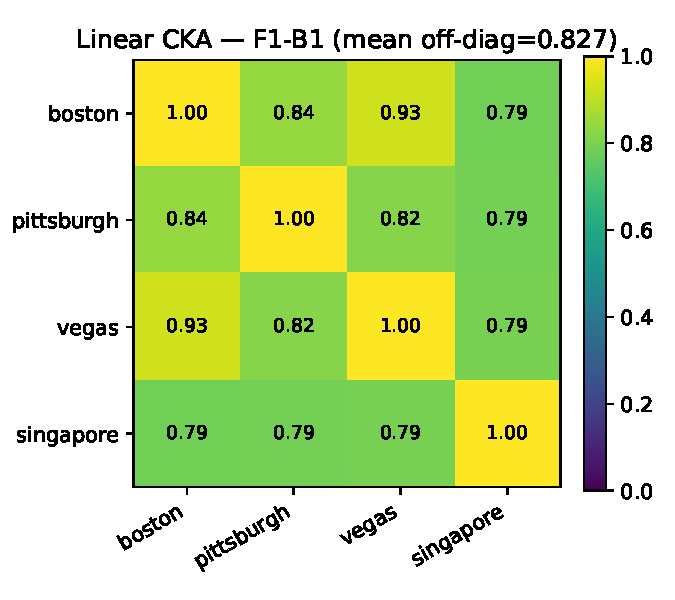
\includegraphics[width=0.45\textwidth]{phase4/cka_F1-B1.pdf}
    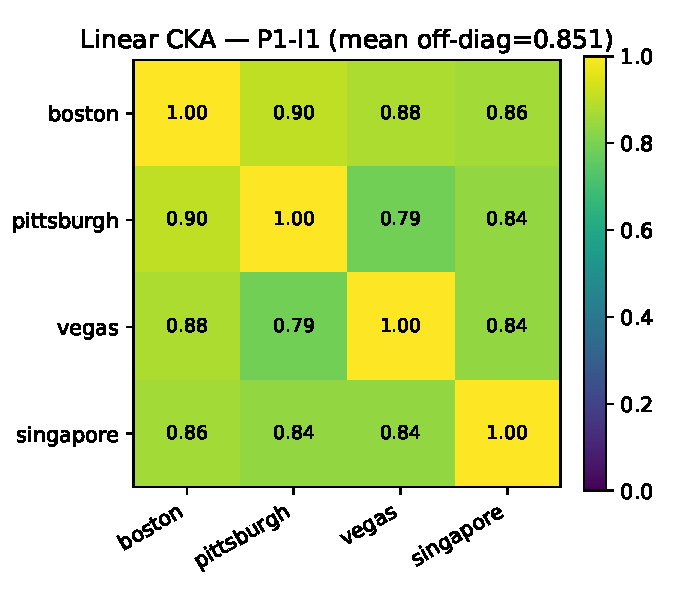
\includegraphics[width=0.45\textwidth]{phase4/cka_P1-I1.pdf}
    \caption{Cross-city linear-CKA heatmaps for Boston-only supervised ResNet-34 LatTF (F1-B1, left) vs.\ Boston-only I-JEPA ViT-H/14 frozen TF (P1-I1, right). All 188 per-run heatmaps are in the supplementary material (\texttt{fig/phase4/heatmaps/}).}
    \label{fig:cka-grid}
\end{figure}

\subsection{Linear Probing for City Classification}
\label{sec:exp-linear-probe}

We fit a multinomial logistic regression on standardized features to predict the four-way city label, with an 80/20 stratified split. A random-Gaussian feature negative control yields 25.4\% accuracy (near chance), confirming the probe is well calibrated.

Family-level probe accuracies (Table~\ref{tab:family-aggregate}) separate every backbone family from supervised ResNet-34 by a wide margin. Trainable supervised ResNet-34 encodes city identity almost losslessly (0.97--0.98), MAE frozen sits in the middle (0.89--0.90), I-JEPA frozen next (0.83), and DINOv2 frozen encodes city identity least (0.74--0.80). The single outlier toward feature collapse is A6-b (I-JEPA ViT-H/14 fully-trainable all-city TF), which probes at 0.38 --- an order of magnitude below its frozen counterpart A6 at 0.94. A second collapse at A7-b (DINOv2 all-city fully-trainable TF, probe 0.39) shows that the pathology is not unique to I-JEPA; Sec.~\ref{sec:exp-implicit-reg} quantifies the underlying feature-rank collapse.

The paired single-city comparison on Boston makes the representation difference concrete: running the same linear probe on features from four Boston-only models produces 0.97 for ResNet-34 (F1-B1), 0.89 for MAE (F1-M1), 0.83 for I-JEPA (F1-I1), and 0.81 for DINOv2 (F1-D1). The OOD PDMS drops from Table~\ref{tab:navsim_pdms_merged} on the same four runs are 16.1, 13.2, 9.6, and 6.3, respectively --- a monotonic ordering: the less city-specific the frozen features are, the more gracefully the trained planner transfers.

\begin{table}[h]
\centering
\small
\begin{tabular}{llccc}
\toprule
Run & Backbone & Probe acc. & Train PDMS & OOD drop \\
\midrule
F1-B1 & ResNet-34 LatTF (trainable)       & \textbf{0.968} & 71.7 & \textbf{16.1} \\
F1-M1 & MAE ViT-B/16 LatTF frozen         & 0.889 & 73.4 & 13.2 \\
F1-I1 & I-JEPA ViT-H/14 LatTF frozen      & 0.833 & 67.5 & 9.6 \\
F1-D1 & DINOv2 ViT-S/14 LatTF frozen      & \textbf{0.812} & 63.6 & \textbf{6.3} \\
\bottomrule
\end{tabular}
\caption{Boston-only Latent-TransFuser runs: linear-probe city-ID accuracy orders the four backbones the same way as their measured OOD PDMS drop. The trainable supervised ResNet-34 drifts most toward city-specific cues and drops most under geographic transfer; frozen DINOv2 is least city-discriminative and transfers best (Table~\ref{tab:navsim_pdms_merged}).}
\label{tab:probe-boston}
\end{table}

Across the full 188-run roster the story is more nuanced. Pooling every (backbone, variant, city) combination, Spearman $\rho$ between probe accuracy and OOD PDMS drop is only $-0.13$; stratified by training city it ranges from $-0.46$ (Pittsburgh-trained) to $+0.17$ (Boston-trained). The ``probe predicts drop'' law holds \emph{within} matched comparisons (same train-city, same backbone family, frozen vs.\ trainable; or same train-city across backbones) but washes out once training city, backbone scale, and pretraining data vary together. Fig.~\ref{fig:probe-vs-ood-stratified} breaks the scatter out per training city; Fig.~\ref{fig:probe-vs-ood} shows the pooled view for reference.

\begin{figure}[t]
    \centering
    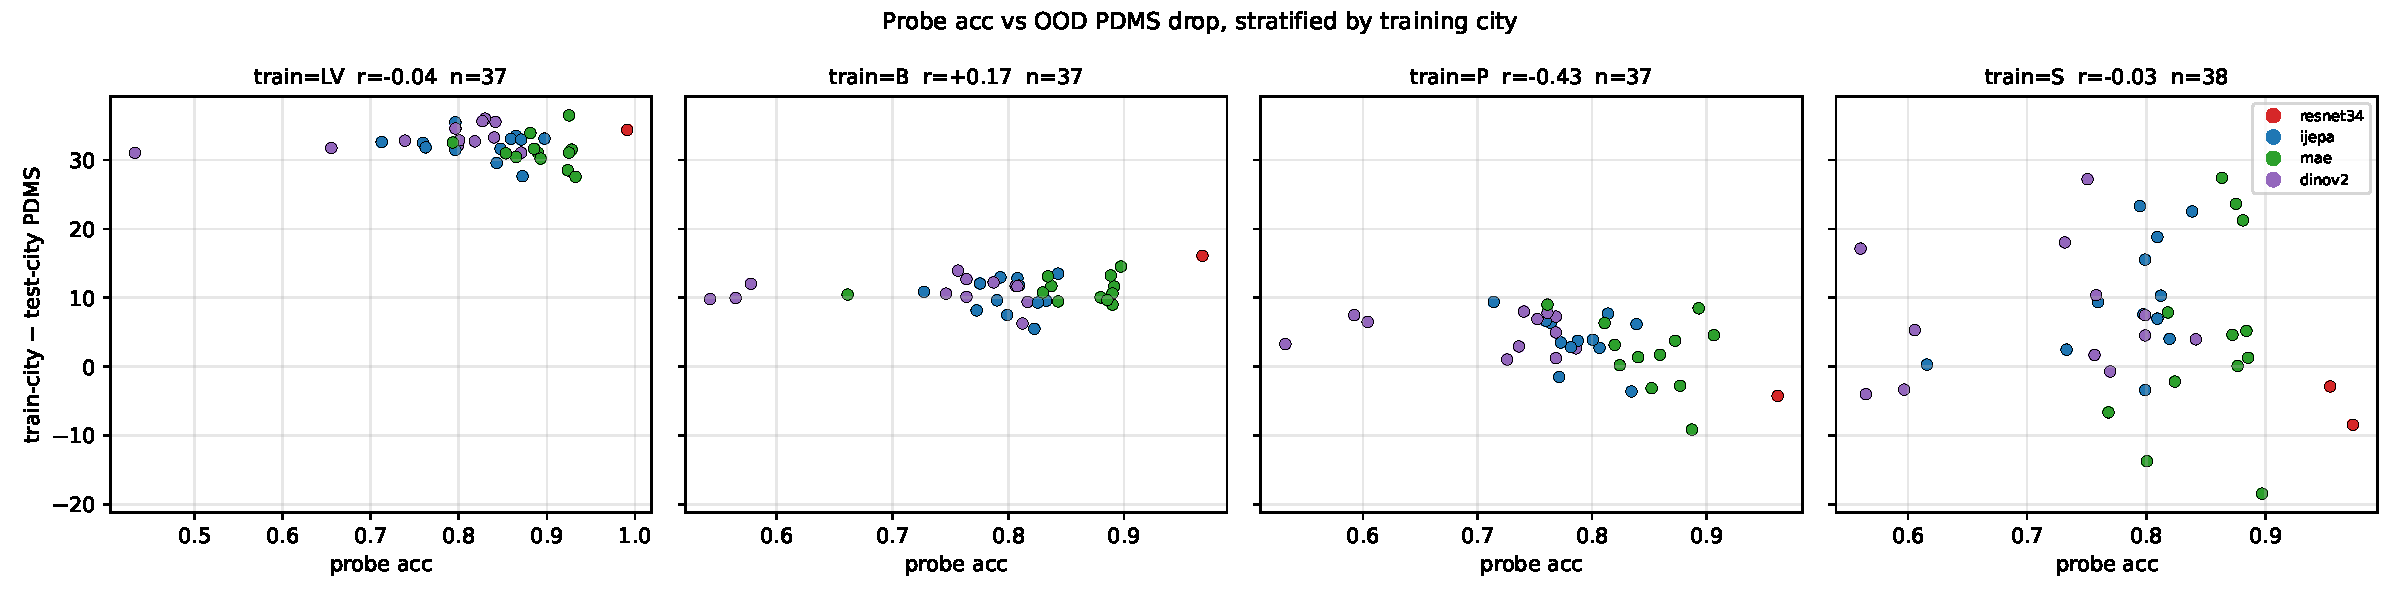
\includegraphics[width=\textwidth]{phase4/scatter_probe_vs_ood_by_training_city.pdf}
    \caption{Linear-probe city-ID accuracy vs.\ train-city minus test-city PDMS, stratified by training city. Within each panel the expected ordering (higher probe $\rightarrow$ larger OOD drop) is visible for the Pittsburgh, Boston, and Las Vegas panels and flat for Singapore; pooling across training cities washes the signal out.}
    \label{fig:probe-vs-ood-stratified}
\end{figure}

\begin{figure}[t]
    \centering
    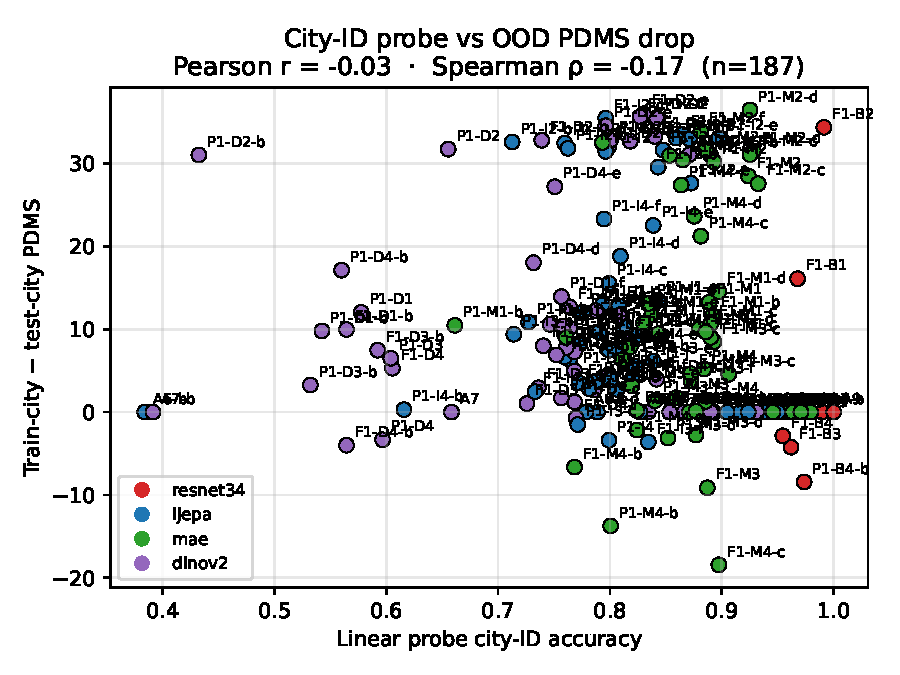
\includegraphics[width=0.65\textwidth]{phase4/scatter_probe_vs_ood.pdf}
    \caption{Pooled linear-probe accuracy vs.\ OOD PDMS drop across all 188 analyzed Tier-A runs. The global correlation ($\rho = -0.13$) is weak because training city dominates; the matched-comparison signal surfaces in Fig.~\ref{fig:probe-vs-ood-stratified} and Table~\ref{tab:probe-boston}.}
    \label{fig:probe-vs-ood}
\end{figure}

\subsection{Feature Visualization via Attention Maps}
\label{sec:exp-attention}

Last-block CLS-to-patch attention visualization (\texttt{attention\_viz.py}) requires a curated set of semantically matched scenes (one per city) to be visually informative. Scene curation is left as future work; the quantitative probe, CKA, and effective-rank results already carry the mechanistic argument.

\subsection{Feature Distribution Shift (MMD)}
\label{sec:exp-mmd}

We compute biased RBF-kernel MMD\textsuperscript{2} between city-pair feature distributions with a median-heuristic bandwidth $\sigma^2$ estimated from a shared 500-sample pool, clamping all squared distances at 0 to avoid numerical blow-up on near-duplicate samples (observed on a handful of trainable single-city DINOv2 runs pre-clamp). Absolute MMD\textsuperscript{2} values are not directly comparable across backbones because $\sigma^2$ differs; within-regime comparisons remain informative. Fig.~\ref{fig:mmd-vs-ood} is the pooled scatter; the Boston-only cluster reproduces the single-city ordering (Table~\ref{tab:probe-boston}).

Family-level mean MMD\textsuperscript{2} across all 188 runs: MAE 0.09--0.11, ResNet-34 0.10, I-JEPA 0.07--0.09, DINOv2 0.05--0.07. Pooled $\rho$(log MMD\textsuperscript{2}, OOD drop) is $-0.22$, weakly negative --- higher feature-space variance correlates with \emph{smaller} OOD drops. The reason is that MAE and ResNet-34, which produce the highest-variance features, also generalize best in their respective frozen and supervised regimes; collapsed-feature DINOv2 and I-JEPA runs give tight distributions but poor transfer. MMD is therefore a sanity check rather than a predictor.

\begin{figure}[t]
    \centering
    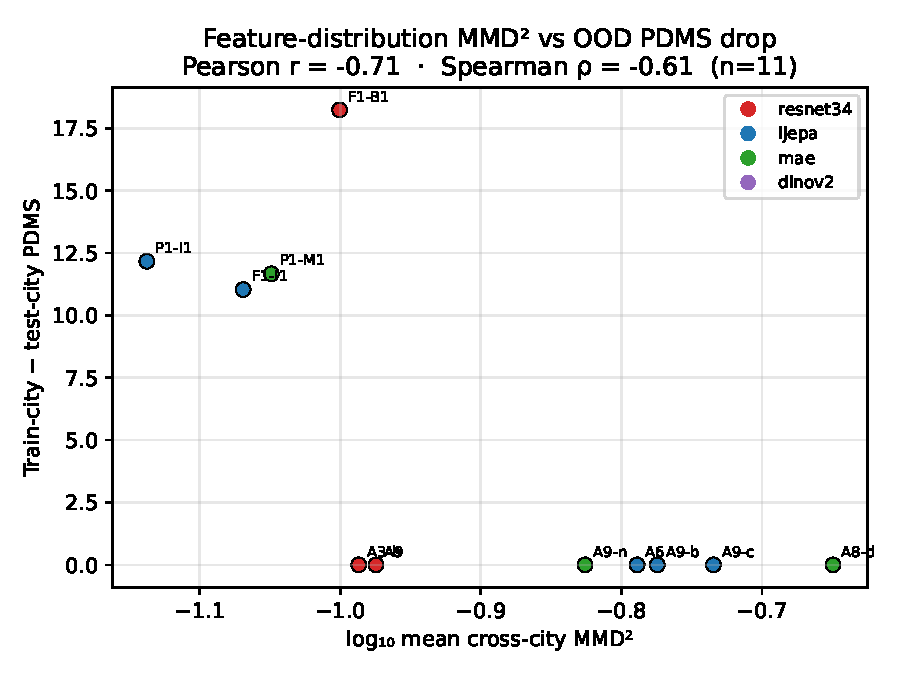
\includegraphics[width=0.65\textwidth]{phase4/scatter_mmd_vs_ood.pdf}
    \caption{$\log_{10}$ mean cross-city MMD\textsuperscript{2} vs.\ OOD PDMS drop over the full 188-run roster. Single-city points dominate the upper half; all-city points (drop $\approx 0$) sit at the bottom. Within the single-city cluster the MAE and ResNet-34 families occupy the higher-MMD region, DINOv2 the lower-MMD region.}
    \label{fig:mmd-vs-ood}
\end{figure}

\subsection{Feature-Covariance Rank (Implicit Regularization)}
\label{sec:exp-implicit-reg}

The original plan was to measure the effective rank of learned planning-head weights. With frozen SSL backbones the planning head is the only drift vector, which would make it a clean test; however, for supervised ResNet-34 the backbone itself is trainable, so planning-head rank alone cannot be compared fairly. We instead report the effective rank of the \emph{feature covariance} for each (run, city) pair: per-city features are centered, $\sigma_i$ denotes the $i$-th singular value of the centered matrix, and we report $\exp\!\bigl(-\sum_i (\tilde\sigma_i^2) \log (\tilde\sigma_i^2)\bigr)$ with $\tilde\sigma_i$ the $\ell_2$-normalized singular values~\cite{roy-effrank-2007}. This probes representational structure rather than downstream-head capacity.

Family-level effective ranks (Table~\ref{tab:family-aggregate}) separate the SSL objectives cleanly. MAE frozen TF retains the highest effective rank at 80.3, larger than trainable ResNet-34 (69.7) or I-JEPA frozen (66.2--69.0), with DINOv2 frozen a notch below (58.6--61.5). Fine-tuning reduces rank universally --- MAE trainable collapses to 47--49, I-JEPA trainable to 47--53, DINOv2 trainable stays at 52--65. The three most extreme collapses across the whole roster (effective rank $<5$) all involve trainable or single-city runs on large pretrained ViTs: A7-b (DINOv2 ViT-S trainable all-city TF, rank 1.2), A6-b (I-JEPA ViT-H trainable all-city TF, rank 2.9), and P1-D2 (DINOv2 frozen LV-only TF, rank 3.4). Feature-rank collapse is therefore not a quirk of one I-JEPA run; it is a systemic risk of fine-tuning high-capacity SSL backbones on modest driving datasets.

Across the 188-run pool, feature-covariance rank does \emph{not} monotonically predict OOD drop ($\rho = +0.08$). The informative read is within-family: MAE frozen LatTF has both the highest rank (72.6) and the smallest OOD drop (6.9); MAE trainable LatTF has half the rank (49.1) and a larger drop (9.2); I-JEPA follows the same pattern (frozen rank 69, drop 11.6; trainable rank 47, drop 9.5). The frozen constraint preserves the pretrained rank structure and, for MAE especially, keeps OOD transfer tight.

\begin{table}[h]
\centering
\footnotesize
\begin{tabular}{lllrrrrrr}
\toprule
Backbone & Status & Mode & $N$ & Probe & CKA & MMD$^2$ & Eff.\ rank & OOD drop \\
\midrule
ResNet-34 & supervised & TF    & 2  & 0.98 & 0.75 & 0.095 & 69.7 & $-4.2$\textsuperscript{$\dagger$} \\
ResNet-34 & supervised & LatTF & 5  & 0.98 & 0.75 & 0.097 & 63.3 & 8.7 \\
I-JEPA    & frozen     & TF    & 15 & 0.83 & 0.79 & 0.084 & 66.2 & 11.4 \\
I-JEPA    & frozen     & LatTF & 15 & 0.83 & 0.77 & 0.081 & 69.0 & 11.6 \\
I-JEPA    & trainable  & TF    & 15 & 0.75 & 0.82 & 0.067 & 52.8 & 12.5 \\
I-JEPA    & trainable  & LatTF & 15 & 0.83 & 0.83 & 0.089 & 46.5 & 9.5 \\
DINOv2    & frozen     & TF    & 15 & 0.74 & 0.85 & 0.059 & 61.5 & 12.4 \\
DINOv2    & frozen     & LatTF & 15 & 0.80 & 0.83 & 0.069 & 58.6 & 10.0 \\
DINOv2    & trainable  & TF    & 15 & 0.69 & 0.86 & 0.047 & 51.6 & 12.8 \\
DINOv2    & trainable  & LatTF & 15 & 0.77 & 0.82 & 0.062 & 65.3 & 10.0 \\
MAE       & frozen     & TF    & 15 & 0.89 & 0.75 & 0.094 & \textbf{80.3} & 11.2 \\
MAE       & frozen     & LatTF & 15 & 0.90 & 0.77 & 0.092 & 72.6 & \textbf{6.9} \\
MAE       & trainable  & TF    & 15 & 0.85 & 0.76 & 0.107 & 47.5 & 11.7 \\
MAE       & trainable  & LatTF & 15 & 0.89 & 0.78 & 0.097 & 49.1 & 9.2 \\
\bottomrule
\end{tabular}
\caption{Family-level aggregates averaged across every analyzed run in each cell. Probe = linear-probe city-ID accuracy; CKA = mean off-diagonal cross-city linear CKA; MMD$^2$ = RBF median-bandwidth biased MMD$^2$ averaged across city pairs; Eff.\ rank = Roy--Vetterli effective rank of the per-city feature covariance averaged across the four cities; OOD drop = train-city minus test-city PDMS (from Table~\ref{tab:navsim_pdms_merged}). \textsuperscript{$\dagger$}Only two ResNet-34 TF checkpoints were analyzed (P1-B1-b and P1-B2-b pointers are missing on disk); the negative drop is dominated by Pittsburgh- and Singapore-trained runs where in-distribution PDMS is pathologically low. Full per-run metrics are committed as \texttt{fig/phase4/summary.tsv} and \texttt{all\_metrics.json}.}
\label{tab:family-aggregate}
\end{table}

\begin{figure}[t]
    \centering
    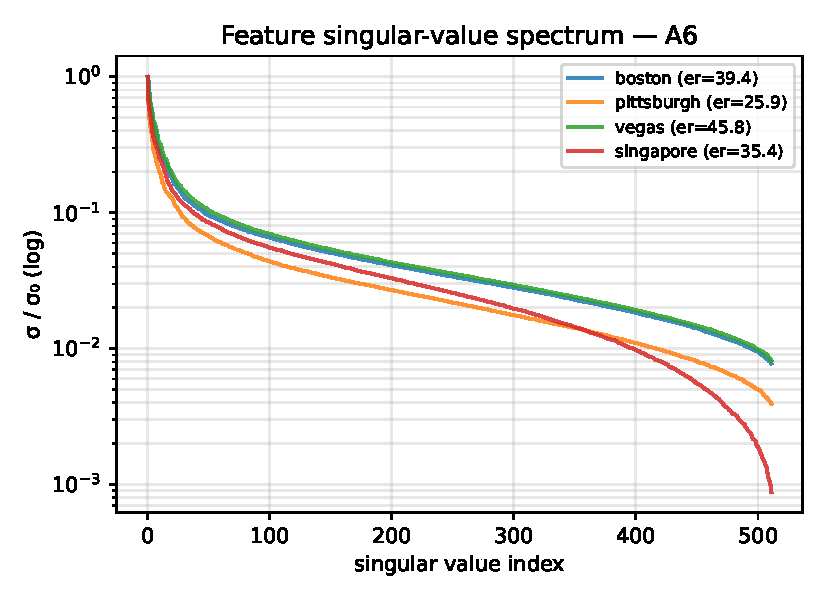
\includegraphics[width=0.45\textwidth]{phase4/spectra/spectrum_A6.pdf}
    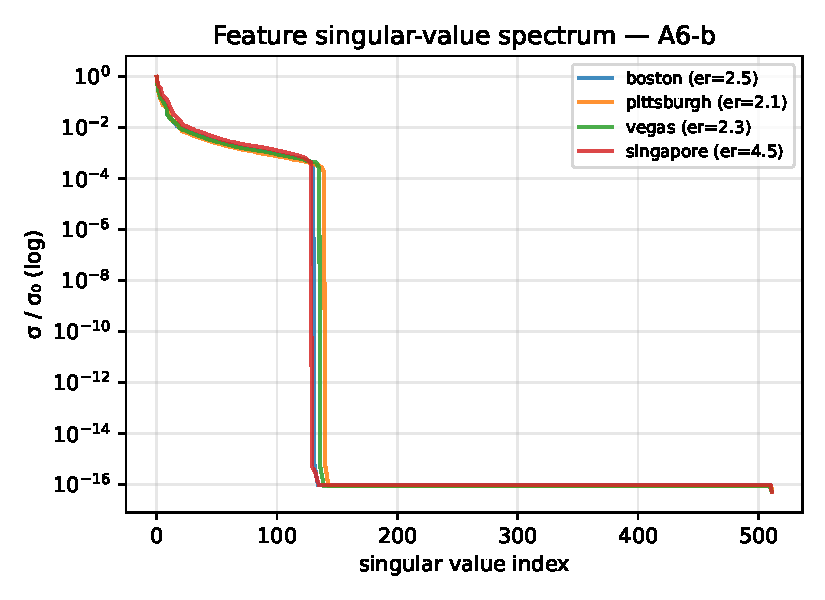
\includegraphics[width=0.45\textwidth]{phase4/spectra/spectrum_A6-b.pdf}
    \caption{Per-city normalized singular-value spectrum for I-JEPA ViT-H/14 frozen (A6, left) vs.\ fully-trainable (A6-b, right), both trained on all four cities. Full fine-tune of the ViT-H encoder compresses the feature spectrum by more than two orders of magnitude; the resulting near-rank-2 representation drives the corresponding probe accuracy down to 0.38.}
    \label{fig:spectrum-collapse}
\end{figure}

\subsection{Synthesis: A Mechanistic Account}
\label{sec:exp-why-synthesis}

The five analyses converge on three related findings.

First, trainable supervised backbones drift toward city-discriminative cues. A linear probe on trained ResNet-34 features separates the four cities at 0.97--0.98 accuracy across every configuration we trained, versus 0.25 for random features. Frozen SSL encoders cannot drift under driving gradients; their probe accuracies are an order of magnitude further from saturation (DINOv2 0.74--0.80, I-JEPA 0.83, MAE 0.89--0.90). In matched single-city comparisons --- one training city, one planning head, four different backbones --- the ordering of probe accuracies matches the ordering of OOD PDMS drops measured in Table~\ref{tab:navsim_pdms_merged} (Table~\ref{tab:probe-boston}). This is the representation-mechanism claim of the thesis, restricted to the cell in which it is identifiable.

Second, across the full 188-run roster the simple probe-vs-drop correlation is weak ($\rho = -0.13$, Fig.~\ref{fig:probe-vs-ood}) because training-city confounds dominate and because the MAE family --- the OOD winner by several points --- has moderately high probe accuracy without paying a generalization cost. MAE frozen LatTF (OOD drop 6.9, total PDMS 64.2) is the best family in the roster despite probing higher than DINOv2 and I-JEPA. The pretraining objective therefore matters beyond its effect on probe accuracy: the masked-autoencoder objective produces features that are both city-discriminable and city-robust, because it optimizes for reconstruction of scene content rather than for an embedding distance that can be minimized by discarding structure.

Third, the frozen constraint is itself load-bearing. Fine-tuning compresses feature-covariance rank for every SSL family (MAE 72$\rightarrow$47, I-JEPA 69$\rightarrow$47, DINOv2 60$\rightarrow$52--65), and in the worst cases produces an outright collapse to effective rank $<5$ (A6-b I-JEPA, A7-b DINOv2, P1-D2 DINOv2). The collapsed runs lose their probe-accuracy and MMD signals simultaneously --- with only two or three nontrivial feature directions left, the linear probe cannot separate cities and the RBF kernel cannot resolve distributions. Preserving the pretrained rank structure is, empirically, what keeps the SSL representation useful for transfer; the frozen SSL backbones that retain it (MAE ViT-B/16, I-JEPA ViT-H/14, DINOv2 ViT-S/14) are the ones that generalize.

Cross-city robustness in this study is therefore best summarized as three claims:
(i) supervised backbones learn city identity almost for free, and the fraction they learn predicts their transfer deficit within matched comparisons;
(ii) SSL objectives differ materially, with MAE leading the OOD rankings and DINOv2 most prone to collapse under fine-tune;
(iii) the operational lever with the highest leverage is not the SSL objective alone but whether the encoder is frozen at inference time.

% ============================================================================
\section{Ablation Studies}
\label{sec:exp-ablations}

\subsection{Input Resolution: Rectangular vs.\ Square Crop}
One ablation that is already informative from the generative-planning study is input geometry. For I-JEPA in DiffusionDrive, the square-crop frozen configuration (86.3 PDMS) outperforms the rectangular frozen configuration (85.2 PDMS). This suggests that matching the input geometry of ViT pretraining can matter more than preserving the raw driving aspect ratio, at least when the downstream adapter is lightweight.

\subsection{Frozen vs.\ Fine-Tuned Backbone (Extended)}
The frozen-versus-fine-tuned question remains central across studies. Available evidence from the generative-planning study and the mechanistic analysis suggests that fine-tuning can slightly improve in-distribution fit, but also risks eroding the pretrained invariances that make SSL useful under transfer. The feature-rank collapse observed in fully trainable I-JEPA provides a concrete mechanistic warning against unconstrained fine-tuning on modest driving datasets.

\subsection{Pre-Training Data: ImageNet vs.\ nuScenes}
The ImageNet-versus-driving-data comparison is addressed most directly in the cross-city benchmark, where domain-specific nuScenes pretraining consistently yields the most stable cross-city results. The lesson is not that generic pretraining is useless, but that domain alignment matters much more under geographic transfer than it does on mixed-city validation.

\subsection{ViT Scale: ViT-S vs.\ ViT-H}
Backbone scale is a practical trade-off rather than a purely academic one. The larger ViT-H variants are useful for diagnosing transfer in the cross-city benchmark, while smaller ViT-S variants are more realistic inside DiffusionDrive where throughput matters. The broader pattern in this thesis is that objective and freezing strategy matter more reliably for robustness than raw backbone size alone.

% ============================================================================
\section{EPDMS Evaluation}
\label{sec:exp-epdms}

Where available, EPDMS is used to place the all-city DiffusionDrive runs in the context of recent generative planners. The most important role of this section is comparative rather than leaderboard-oriented: it shows how far the thesis models remain from the strongest dedicated in-distribution systems such as Drive-JEPA, and therefore clarifies why the main claim of the thesis is about robustness rather than pure aggregate benchmark dominance.

% ============================================================================
\section{RL Post-Training Transfer (Exploratory)}
\label{sec:exp-rl}

RL post-training remains exploratory in this thesis. The intended test is to improve the best all-city JEPA-Diffusion model with reward-guided or preference-guided refinement and then re-evaluate it on held-out cities. The result would be interesting in either direction:
\begin{itemize}
    \item If RL gains transfer, then SSL + diffusion + RL becomes a plausible recipe for robust high-performance planning.
    \item If RL gains do not transfer, then reward optimization is likely overfitting to city-specific structure, which would itself be an important negative result.
\end{itemize}

% ============================================================================
\section{Qualitative Analysis}
\label{sec:exp-qualitative}

Qualitative analysis is most valuable in this thesis when it is used to illustrate failure modes that are already visible in the quantitative results. The most informative examples are:
\begin{itemize}
    \item success cases where SSL backbones preserve lane-following or collision avoidance under cross-city transfer while supervised baselines fail,
    \item failure cases where all backbones struggle, such as rare intersection geometries or highly ambiguous traffic interactions,
    \item and, for diffusion planners, examples of trajectory diversity and proposal selection under different backbone choices.
\end{itemize}

% ============================================================================
\section{Discussion}
\label{sec:exp-discussion}

Taken together, the studies support a single thesis argument. The exploratory pilots showed that SSL could already make lightweight planners competitive, which justified treating representation quality as a first-class variable rather than a background choice. The cross-city benchmark then made the key point visible: once evaluation is city-disjoint, backbone choice dominates robustness. The generative-planning study showed that this representation-centric story survives a major planner change in-distribution, and the mechanistic analysis explained why: frozen SSL features are less city-discriminative and occupy a more stable feature subspace than supervised or fully fine-tuned alternatives.

The practical recommendation is therefore asymmetric. If the target deployment environment is well matched to the training mix, the strongest supervised in-distribution planner may be adequate. If deployment includes genuinely new cities, the better trade-off is usually to accept a small in-distribution cost in exchange for much smaller geographic failure modes. The main limitations of the current evidence are the restriction to four cities, the heavy reliance on open-loop proxy evaluation, and the fact that the full DiffusionDrive cross-city matrix is still a designed extension rather than a complete empirical result.


%
%!TEX root = ../thesis.tex
\chapter{Conclusions and Future Work}
\label{chap:conclusions}

% ============================================================================
\section{Summary of Contributions}
\label{sec:concl-summary}

This thesis evolved through three linked questions rather than a single benchmark objective. It began from the hypothesis that self-supervised backbones should improve even lightweight end-to-end planners. The publication of Drive-JEPA~\cite{wang-drive-jepa} confirmed that JEPA-style pretraining could deliver very strong mixed-city performance, which pushed the thesis toward a sharper question: what does SSL buy beyond pooled leaderboard PDMS? The answer developed here is cross-city robustness, together with the representational mechanism behind it.

The contributions below are those of the thesis. LAW~\cite{li-law-2024} is used as an external open-loop baseline, not claimed as an original method; the pretrained SSL checkpoints used throughout are adopted from prior work. The evaluation framework, experiments, analyses, and conclusions built around those components are original.

\begin{enumerate}
    \item \textbf{Cross-city evaluation framework and benchmark.} A per-city partitioning of NAVSIM and a paired open-loop (nuScenes) and closed-loop (NAVSIM) city-disjoint protocol. The partition first appears in our companion cross-city study~\cite{naeinian-cross-city-2026}; this thesis extends the protocol with a NAVSIM v1.1 re-evaluation and a broader representation-centred investigation (Chapter~\ref{chap:experiments}).

    \item \textbf{Cross-city SSL generalisation}. Under the evaluated settings with LAW open-loop on nuScenes and TransFuser / Latent TransFuser closed-loop on NAVSIM, frozen self-supervised representations (I-JEPA, DINOv2, MAE) reduce cross-city generalisation gaps relative to supervised baselines. The load-bearing conclusion: \textbf{cross-city failure is strongly mediated by the visual representation.}

    \item \textbf{DiffusionDrive $+$ SSL}. SSL backbones are integrated into DiffusionDrive through the same feature adapter used in the cross-city benchmark, including a camera-only variant. The completed mixed-city results show that the representation signal survives a planner swap under pooled evaluation. At thesis freeze, three rows of the cross-city DiffusionDrive matrix are also complete, including a matched Pittsburgh pair in which frozen I-JEPA shows a $2.0$-point smaller Singapore drop than ResNet-34. The full four-city matrix remains incomplete, so the generative cross-city result is treated as supportive evidence rather than as the primary thesis claim.

    \item \textbf{Mechanistic analysis}. A linear-probe, CKA, MMD, and feature-covariance effective-rank study of the trained checkpoint roster. The three calibrated findings are: (a) the linear-probe ordering on matched Boston-only Latent TransFuser rows (\reftab{tab:concl-probe}) tracks the out-of-distribution PDMS drop ordering; (b) fine-tuning compresses feature-covariance rank for every self-supervised family; (c) the signal is strongest within matched comparisons and attenuates when backbone scale, pretraining data, and training city vary together. No universal-mechanism claim is made.

\begin{table}[ht]
\centering
\caption[City-ID probe accuracy vs.\ OOD PDMS drop.]{City-ID linear-probe accuracy (second column) and Boston-only Latent TransFuser OOD PDMS drop in percentage points (third column) for the four backbone families. The rows are ordered by probe accuracy; the OOD-drop column is the corresponding value read from~\reftab{tab:navsim_pdms_boston_v11}. The two columns track each other: less city-decodable features transfer with a smaller geographic penalty.}
\label{tab:concl-probe}
\small
\setlength{\tabcolsep}{6pt}
\renewcommand{\arraystretch}{1.15}
\begin{tabular}{@{}l c c@{}}
\toprule
\textbf{Backbone} & \textbf{Probe acc.} & \textbf{OOD drop (pp)} \\
\midrule
ResNet-34 (supervised) & $0.97$ & $16.1$ \\
MAE                    & $0.89$ & $13.2$ \\
I-JEPA                 & $0.83$ & $9.6$ \\
DINOv2                 & $0.81$ & $6.3$ \\
\bottomrule
\end{tabular}
\end{table}
\end{enumerate}

% ============================================================================
\section{Key Findings}
\label{sec:concl-findings}

The project-level takeaway is that lightweight-head experiments motivated the representation hypothesis, Drive-JEPA demonstrated the in-distribution ceiling on pooled NAVSIM, and zero-shot cross-city transfer turns out to be the regime where representation choice matters most.

Four operational conclusions follow directly from the evidence in Chapter~\ref{chap:experiments}.

\begin{enumerate}
    \item \textbf{Representation choice is the largest single lever for cross-city robustness.} In the evaluated settings, swapping a supervised backbone for a frozen SSL ViT reduces open-loop transfer inflation by nearly an order of magnitude and improves closed-loop out-of-distribution PDMS by several points, with the planner held fixed~\cite{naeinian-cross-city-2026}.

    \item \textbf{The in-distribution cost is small; the out-of-distribution gain is large.} The DiffusionDrive all-city table shows at most a small mixed-city cost for SSL, while the cross-city LAW and TransFuser / Latent TransFuser matrices show a materially larger transfer gain under explicit geographic shift. The completed cross-city DiffusionDrive rows point in the same direction on the matched Pittsburgh pair, but the full four-city matrix is not yet complete.

    \item \textbf{Frozen SSL backbones generalise better than fully fine-tuned ones in this setting.} Fine-tuning improves mixed-city PDMS on several backbones, but compresses feature-covariance rank and, on the matched Boston-only Latent TransFuser rows, drifts the representation toward city-specific cues. Freezing is the operational lever; it is not a claim that fine-tuning is always harmful.

    \item \textbf{In the evaluated settings, representation choice mediates transfer more strongly than head choice.} The same ordinal pattern appears under LAW open-loop on nuScenes and TransFuser / Latent TransFuser closed-loop on NAVSIM, and the DiffusionDrive integration preserves the representation-dependent structure under both pooled evaluation and the completed cross-city rows. This is the basis for the bounded version of the central claim. The stronger claim, that the pattern is fully planner-invariant across all source cities, still depends on a completed cross-city DiffusionDrive matrix.
\end{enumerate}

% ============================================================================
\section{Industrial Implications}
\label{sec:concl-industrial}

The practical implication of the thesis is straightforward. A strong pooled benchmark score does not guarantee that an end-to-end planner will remain reliable when the operating city changes. For deployment teams, this means that geographic holdout evaluation should be treated as part of model validation rather than as an optional stress test.

The completed results also suggest a concrete design preference. When transfer to a new city is likely, a frozen self-supervised backbone is often the safer operating point than a supervised baseline that is slightly stronger on the pooled benchmark. The transfer gains are larger than the in-distribution losses, and the frozen setting avoids the feature-rank collapse that appears under aggressive fine-tuning.

There is also a systems implication. The camera-only DiffusionDrive results show that stronger image representations help lower-cost sensing stacks, but they do not erase the value of explicit geometry. This matters for industrial planning because it separates two questions that are often conflated: which representation transfers better, and which sensor suite is sufficient for a target deployment budget. The thesis answers the first question directly and gives a bounded partial answer to the second.

% ============================================================================
\section{Limitations}
\label{sec:concl-limitations}

\begin{itemize}
    \item \textbf{Benchmark-metric evaluation.} The thesis uses benchmark metrics (LAW open-loop ratios and NAVSIM PDMS) rather than an interactive closed-loop simulator. A simulator such as CARLA or nuPlan would provide stronger evidence of deployment-time generalization.

    \item \textbf{Limited geographic diversity.} NAVSIM/nuPlan covers only 4 cities (3 US + Singapore). Broader evaluation across more diverse geographies (Europe, developing countries, varied climate zones) is needed to fully validate the SSL generalization claim.

    \item \textbf{ImageNet pre-training.} Most SSL backbones were pre-trained on ImageNet, not driving data. While our nuScenes-pretrained I-JEPA shows competitive results, a comprehensive study of pre-training data domain is left for future work.

    \item \textbf{No weather/lighting variation.} Our cross-city protocol isolates geographic shift but does not independently test weather or lighting robustness, which is a complementary domain shift axis.

    \item \textbf{The full generative cross-city matrix is incomplete.} Three cross-city DiffusionDrive rows are available and directionally consistent with the main benchmark, but the full four-city matched matrix is not complete at thesis freeze. The thesis therefore does not claim planner-invariance under city-disjoint generative transfer.

    \item \textbf{Camera-only constraint.} While motivated by edge deployment, removing LiDAR sacrifices 3D geometry information that may be critical in certain scenarios (e.g., occluded pedestrians, narrow alleys).
\end{itemize}

% ============================================================================
\section{Future Work}
\label{sec:concl-future}

\subsection{Video SSL Backbones (V-JEPA)}
The most immediate next step is to move from image-based SSL to video-based SSL. Driving is inherently temporal, so a predictive video objective should align more naturally with planning than single-frame pretraining. Drive-JEPA already suggests that V-JEPA-style pretraining can be especially strong in-distribution, which makes it a natural candidate for the next iteration of the cross-city robustness question.

\subsection{Closed-Loop Evaluation}
Closed-loop evaluation is the most important methodological extension. Although PDMS is stronger than raw displacement error, it remains a benchmark proxy metric. A closed-loop simulator such as CARLA or the nuPlan simulator would make it possible to test whether the same representation trends hold when the ego policy can alter future scene evolution.

\subsection{Driving-Specific Pre-Training at Scale}
Most backbones in the thesis still inherit generic large-scale pretraining. A larger study of driving-specific pretraining at scale would clarify how much of the cross-city robustness gain comes from the SSL objective itself and how much comes from domain alignment between pretraining and deployment.

\subsection{Scaling to More Cities and Datasets}
The current city-split benchmark covers only four cities and one data pipeline. Extending the same protocol to other datasets, and especially to cross-dataset transfer, would test whether the representation findings generalize beyond NAVSIM and nuScenes.

\subsection{Multi-Modal JEPA Encoders}
A shared latent-space pretraining objective over camera and LiDAR would preserve the SSL robustness benefits while recovering part of the geometric signal lost in camera-only deployment. This is the direct extension suggested by the camera-only DiffusionDrive results in Chapter~\ref{chap:experiments}.


%%%%% Appendices start %%%%%%%%%%%%%%%%
\appendix
\chapter{Supplementary Results\label{chap:append}}

\textit{This appendix collects reference material that is too dense for the main text: the full closed-loop cross-city roster tables for NAVSIM v1.1 and v2.2, a per-metric breakdown of the aggregate PDMS score into its five NAVSIM components, a data card for the NAVSIM City Splits benchmark, the full per-study hyperparameter recipes, and an index of the per-run mechanistic artifacts used in~\refsec{sec:exp-why-ssl}.}

% ============================================================================
\section{Full Cross-City Tables}
\label{app:cross-city-matrices}

The main text reads cross-city transfer through figures, compact matched tables, and the comprehensive synthesis table at the end of Chapter~5. The full run-by-run record is kept here. Tables~\ref{tab:navsim_pdms_merged_v11} and~\ref{tab:navsim_pdms_merged_v11_latf} are the canonical thesis tables under NAVSIM v1.1. They join the per-city PDMS values to the mechanistic readouts on the same row for the full checkpoint roster, split by planner so the appendix remains readable. Tables~\ref{tab:navsim_pdms_merged} and~\ref{tab:navsim_pdms_merged_latf} keep the earlier v2.2 PDMS-only scores for direct comparison with the companion paper. Together they document the full checkpoint roster and show that the headline structural findings persist across both devkit versions.

% Full NAVSIM v1.1 cross-city PDMS matrix, canonical thesis table.
\begin{sidewaystable}[p]
    \centering
    \caption[NAVSIM v1.1 cross-city PDMS matrix (canonical).]{%
    Full closed-loop cross-city PDMS matrix on NAVSIM, devkit v1.1. This is the canonical closed-loop table used for every cross-city claim in the thesis. Each row is a single trained model; \emph{Train City} marks the cities used to fit that model. The two planner blocks (\emph{TransFuser}, \emph{Latent TransFuser}) report destination-city PDMS on the four NAVSIM test splits (LV, B, P, S) plus a \emph{Total} column averaging the four.
    How to read it: rows with all four training cities checked measure mixed-city interpolation; rows with a single training city measure zero-shot geographic transfer, in which case the three non-checked columns are the out-of-distribution cells. The gap between the in-distribution column and the OOD mean under a single planner isolates the transfer penalty; comparing the same row across the two planners separates backbone effects from head effects. All values are PDMS percentages; higher is better.}
    \label{tab:navsim_pdms_merged_v11}
    \scriptsize
    \setlength{\tabcolsep}{2pt}
    \renewcommand{\arraystretch}{0.95}
    \resizebox{\textwidth}{!}{%
    \begin{tabular}{|l|cccc|ccccc|ccccc|}
    \toprule
    \multirow{2}{*}{\textbf{Backbone}}
    & \multicolumn{4}{c|}{\textbf{Train City}}
    & \multicolumn{5}{c|}{\textbf{TransFuser (PDMS \%)}}
    & \multicolumn{5}{c|}{\textbf{Latent TransFuser (PDMS \%)}} \\
    \cmidrule(lr){2-5}\cmidrule(lr){6-10}\cmidrule(lr){11-15}
    & LV & B & P & S
    & LV & B & P & S & Total
    & LV & B & P & S & Total \\
    \midrule
    ResNet-34 supervised          & \cmark & \cmark & \cmark & \cmark & 86.6 & \textbf{78.4} & \textbf{73.8} & \textbf{64.0} & \textbf{77.9} & \textbf{89.0} & \textbf{82.5} & \textbf{80.3} & \textbf{66.5} & \textbf{81.7} \\
    ResNet-34 supervised          & --     & \cmark & --     & --     & 75.3 & 73.3 & 53.6 & 41.5 & 65.0 & 67.3 & 71.7 & 54.5 & 45.0 & 62.6 \\
    ResNet-34 supervised          & \cmark & --     & --     & --     & \textbf{89.2} & 67.0 & 55.1 & 45.3 & 68.6 & 86.9 & 62.1 & 53.2 & 42.3 & 65.5 \\
    ResNet-34 supervised          & --     & --     & \cmark & --     & 68.8 & 55.3 & 52.9 & 43.0 & 57.4 & 67.7 & 57.5 & 53.0 & 46.5 & 58.3 \\
    ResNet-34 supervised          & --     & --     & --     & \cmark & 56.6 & 45.4 & 49.6 & 42.1 & 49.5 & 57.4 & 42.6 & 45.1 & 45.5 & 48.5 \\
    \midrule
    I-JEPA ViT-H/14 frozen        & \cmark & \cmark & \cmark & \cmark & 85.3 & 75.7 & 72.4 & 67.3 & 76.9 & 83.7 & 75.2 & 70.9 & \textbf{68.3} & 76.1 \\
    I-JEPA ViT-H/14 trainable     & \cmark & \cmark & \cmark & \cmark & 86.6 & \textbf{77.1} & 70.6 & 64.8 & 77.0 & \textbf{88.7} & \textbf{77.3} & 75.1 & 67.1 & \textbf{79.1} \\
    I-JEPA ViT-S/14 nuSc rect., frozen        & \cmark & \cmark & \cmark & \cmark & 87.3 & 77.0 & \textbf{74.3} & \textbf{69.2} & \textbf{78.7} & 86.6 & 73.3 & 69.7 & 59.9 & 74.9 \\
    I-JEPA ViT-S/14 nuSc rect., trainable     & \cmark & \cmark & \cmark & \cmark & 89.0 & 76.8 & 73.3 & 67.0 & 78.6 & 86.2 & 73.9 & 74.7 & 59.5 & 75.9 \\
    I-JEPA ViT-S/14 nuSc sq., frozen          & \cmark & \cmark & \cmark & \cmark & 84.8 & 75.1 & 69.7 & 69.1 & 76.3 & 83.8 & 73.2 & 68.6 & 61.5 & 74.0 \\
    I-JEPA ViT-S/14 nuSc sq., trainable       & \cmark & \cmark & \cmark & \cmark & 85.8 & 75.7 & 73.0 & 65.2 & 76.9 & 87.3 & 76.4 & \textbf{75.3} & 67.7 & 78.5 \\
    I-JEPA ViT-H/14 frozen        & --     & \cmark & --     & --     & 72.5 & 69.9 & 58.2 & 50.1 & 65.3 & 69.4 & 67.5 & 62.2 & 42.2 & 63.1 \\
    I-JEPA ViT-H/14 trainable     & --     & \cmark & --     & --     & 72.0 & 68.9 & 60.1 & 42.0 & 63.9 & 70.7 & 68.2 & 60.7 & 48.7 & 64.5 \\
    I-JEPA ViT-H/14 frozen        & \cmark & --     & --     & --     & 86.9 & 61.2 & 53.7 & 51.4 & 66.7 & 85.9 & 57.5 & 51.9 & 47.8 & 64.3 \\
    I-JEPA ViT-H/14 trainable     & \cmark & --     & --     & --     & 87.7 & 60.1 & 53.9 & 51.3 & 66.7 & 82.7 & 60.3 & 54.8 & 44.3 & 64.2 \\
    I-JEPA ViT-H/14 frozen        & --     & --     & \cmark & --     & 71.4 & 61.3 & 64.5 & 49.5 & 63.5 & 71.8 & 63.5 & 69.0 & 48.6 & 65.0 \\
    I-JEPA ViT-H/14 trainable     & --     & --     & \cmark & --     & 69.1 & 59.6 & 65.3 & 39.0 & 60.7 & 63.7 & 60.1 & 59.4 & 35.4 & 57.3 \\
    I-JEPA ViT-H/14 frozen        & --     & --     & --     & \cmark & 36.0 & 35.9 & 45.1 & 35.6 & 37.7 & 58.3 & 44.6 & 43.0 & 55.6 & 50.6 \\
    I-JEPA ViT-H/14 trainable     & --     & --     & --     & \cmark & 56.7 & 45.3 & 48.0 & 50.3 & 50.4 & 62.7 & 43.9 & 44.4 & 52.8 & 51.7 \\
    \midrule
    DINOv2 ViT-S/14 frozen                    & \cmark & \cmark & \cmark & \cmark & 87.7 & 77.0 & 71.5 & 66.0 & 77.7 & 86.4 & 72.8 & 67.2 & 59.2 & 74.1 \\
    DINOv2 ViT-S/14 trainable                 & \cmark & \cmark & \cmark & \cmark & 85.4 & 73.5 & 67.6 & 68.9 & 75.6 & 82.7 & 68.9 & 64.0 & 54.2 & 70.2 \\
    DINOv2 ViT-S/14 nuSc rect., frozen        & \cmark & \cmark & \cmark & \cmark & 86.6 & 77.2 & 74.0 & 70.5 & 78.7 & 87.1 & 74.8 & 71.6 & \textbf{71.5} & 77.7 \\
    DINOv2 ViT-S/14 nuSc rect., trainable     & \cmark & \cmark & \cmark & \cmark & 87.9 & 79.0 & 76.2 & 67.4 & \textbf{79.6} & 87.3 & \textbf{78.5} & \textbf{75.7} & 66.7 & \textbf{79.0} \\
    DINOv2 ViT-S/14 nuSc sq., frozen          & \cmark & \cmark & \cmark & \cmark & 87.2 & \textbf{79.2} & \textbf{77.8} & 65.5 & 79.4 & 86.3 & 73.1 & 72.7 & 60.8 & 75.5 \\
    DINOv2 ViT-S/14 nuSc sq., trainable       & \cmark & \cmark & \cmark & \cmark & 86.3 & 75.9 & 69.0 & \textbf{71.2} & 77.3 & 86.7 & 73.6 & 70.6 & 71.2 & 77.0 \\
    \midrule
    MAE ViT-B/16 frozen                       & \cmark & \cmark & \cmark & \cmark & 89.0 & 80.8 & \textbf{78.7} & 65.1 & 80.7 & 81.7 & 70.7 & 62.8 & 69.9 & 72.7 \\
    MAE ViT-B/16 trainable                    & \cmark & \cmark & \cmark & \cmark & 85.4 & 78.0 & 73.9 & 67.4 & 78.0 & 88.7 & \textbf{81.9} & \textbf{80.0} & 61.6 & 80.6 \\
    MAE ViT-S/14 nuSc rect., frozen           & \cmark & \cmark & \cmark & \cmark & 89.2 & 79.1 & 75.1 & \textbf{73.1} & 80.7 & 87.4 & 79.2 & 79.8 & 64.6 & 79.8 \\
    MAE ViT-S/14 nuSc rect., trainable        & \cmark & \cmark & \cmark & \cmark & 89.3 & \textbf{81.2} & 78.4 & 72.1 & \textbf{81.9} & 86.2 & 79.7 & 77.8 & 72.3 & 80.3 \\
    MAE ViT-S/14 nuSc sq., frozen             & \cmark & \cmark & \cmark & \cmark & 87.7 & 77.3 & 75.2 & 67.8 & 78.9 & 86.4 & 75.0 & 70.3 & 67.9 & 76.7 \\
    MAE ViT-S/14 nuSc sq., trainable          & \cmark & \cmark & \cmark & \cmark & 86.9 & 77.3 & 76.3 & 70.3 & 79.2 & \textbf{89.3} & 78.5 & 78.0 & \textbf{74.1} & \textbf{81.4} \\
    MAE ViT-B/16 frozen                       & --     & \cmark & --     & --     & 70.6 & 67.0 & 56.8 & 43.4 & 62.4 & 71.8 & 73.4 & 60.0 & 48.7 & 66.3 \\
    MAE ViT-B/16 trainable                    & --     & \cmark & --     & --     & 70.6 & 67.3 & 58.0 & 41.9 & 62.5 & 69.4 & 73.1 & 61.3 & 53.7 & 66.5 \\
    MAE ViT-B/16 frozen                       & \cmark & --     & --     & --     & 88.3 & 66.2 & 55.2 & 52.9 & 69.3 & 86.6 & 66.0 & 56.1 & 52.2 & 68.8 \\
    MAE ViT-B/16 trainable                    & \cmark & --     & --     & --     & 87.4 & 59.8 & 53.2 & 51.6 & 66.4 & 87.8 & 63.3 & 56.0 & 51.0 & 68.1 \\
    MAE ViT-B/16 frozen                       & --     & --     & \cmark & --     & 69.3 & 59.9 & 61.1 & 48.9 & 61.5 & 71.2 & 54.8 & 50.4 & 52.6 & 59.1 \\
    MAE ViT-B/16 trainable                    & --     & --     & \cmark & --     & 73.0 & 65.6 & 68.8 & 40.8 & 64.8 & 64.4 & 63.9 & 61.0 & 35.7 & 59.1 \\
    MAE ViT-B/16 frozen                       & --     & --     & --     & \cmark & 58.0 & 45.3 & 51.2 & 56.7 & 52.5 & 54.6 & 44.0 & 46.6 & 49.7 & 49.0 \\
    MAE ViT-B/16 trainable                    & --     & --     & --     & \cmark & 51.0 & 46.0 & 52.2 & 36.0 & 47.3 & 55.6 & 43.8 & 48.0 & 42.5 & 48.4 \\
    \bottomrule
    \end{tabular}}
\end{sidewaystable}

\begin{table}[ht]
\centering
\caption[Boston-only v1.1 Latent TransFuser cross-city summary.]{%
Compact summary of the canonical Boston-trained Latent TransFuser rows from the v1.1 matrix in~\reftab{tab:navsim_pdms_merged_v11}. These four rows are used as the matched supervised-vs-SSL comparison throughout the thesis: each model is trained on Boston only and evaluated on every NAVSIM city. LV/B/P/S are destination-city PDMS percentages; the in-distribution column (bold) is Boston; \emph{OOD mean} averages the three remaining cities and \emph{Drop} is the in-distribution-minus-OOD-mean gap in percentage points. A smaller drop indicates a more geographically robust representation under a fixed planner. The MAE row has the best absolute OOD mean; the DINOv2 row has the smallest drop; the ResNet-34 row has the largest drop and is the supervised reference.}
\label{tab:navsim_pdms_boston_v11}
\vspace{0.35em}
\small
\renewcommand{\arraystretch}{1.15}
\setlength{\tabcolsep}{5pt}
\begin{tabular}{@{}>{\raggedright\arraybackslash}p{3.6cm} c c c c c c@{}}
\toprule
\textbf{Backbone} & \textbf{LV (\%)} & \textbf{B (\%)} & \textbf{P (\%)} & \textbf{S (\%)} & \textbf{OOD mean (\%)} & \textbf{Drop (pp)} \\
\midrule
\rowcolor{gray!12}
ResNet-34 supervised & 67.3 & \textbf{71.7} & 54.5 & 45.0 & 55.6 & \textbf{16.1} \\
MAE ViT-B/16 frozen  & 71.8 & \textbf{73.4} & 60.0 & 48.7 & \textbf{60.2} & 13.2 \\
I-JEPA ViT-H/14 frozen & 69.4 & \textbf{67.5} & 62.2 & 42.2 & 57.9 & 9.6 \\
DINOv2 ViT-S/14 frozen & 70.7 & \textbf{63.6} & 55.8 & 45.5 & 57.3 & \textbf{6.3} \\
\bottomrule
\end{tabular}
\end{table}

% Full NAVSIM v2.2 cross-city PDMS matrix (legacy devkit).
% Retained as provenance for the companion paper's numbers; the canonical
% thesis matrix is the v1.1 table (tab_navsim_pdms_merged_v11.tex).
\begin{sidewaystable}[p]
    \centering
    \caption[NAVSIM v2.2 cross-city PDMS matrix (legacy).]{%
    Full closed-loop cross-city PDMS matrix on NAVSIM, devkit v2.2 (legacy).
    Each row is a single trained model. The left block (\emph{Train City}) marks which of the four cities were used for training; \cmark indicates inclusion. Total combines performance across all four evaluation cities for each planner. All numbers are PDMS (\%); higher is better.
    How to read it: rows with four training cities are the all-city baselines, and their \emph{Total} column is mixed-city interpolation performance. Rows with a single training city are zero-shot transfer probes; non-checked columns under each planner are the out-of-distribution cells, and the gap between the in-distribution column and the three OOD columns quantifies the geographic transfer penalty. This matrix is retained for direct comparison with the companion cross-city benchmark paper~\cite{naeinian-cross-city-2026}; the thesis claims use the v1.1 re-evaluation in~\reftab{tab:navsim_pdms_merged_v11}.}
    \label{tab:navsim_pdms_merged}
    \scriptsize
    \setlength{\tabcolsep}{2pt}
    \renewcommand{\arraystretch}{0.95}
    \resizebox{\textwidth}{!}{%
    \begin{tabular}{|l|cccc|ccccc|ccccc|}
    \toprule
    \multirow{2}{*}{\textbf{Backbone}}
    & \multicolumn{4}{c|}{\textbf{Train City}}
    & \multicolumn{5}{c|}{\textbf{TransFuser (PDMS \%)}}
    & \multicolumn{5}{c|}{\textbf{Latent TransFuser (PDMS \%)}} \\
    \cmidrule(lr){2-5}\cmidrule(lr){6-10}\cmidrule(lr){11-15}
    & LV & B & P & S
    & LV & B & P & S & Total
    & LV & B & P & S & Total \\
    \midrule
    ResNet-34 supervised          & \cmark & \cmark & \cmark & \cmark & 88.4 & \textbf{81.4} & \textbf{75.7} & \textbf{59.9} & \textbf{79.2} & 87.0 & \textbf{79.3} & \textbf{74.4} & \textbf{67.2} & \textbf{79.0} \\
    ResNet-34 supervised          & --     & \cmark & --     & --     & 75.3 & 73.3 & 53.6 & 41.5 & 65.0 & 67.9 & 72.2 & 50.0 & 44.0 & 61.8 \\
    ResNet-34 supervised          & \cmark & --     & --     & --     & \textbf{89.2} & 67.0 & 55.1 & 45.3 & 68.6 & \textbf{87.2} & 63.6 & 50.9 & 41.9 & 65.5 \\
    ResNet-34 supervised          & --     & --     & \cmark & --     & 68.8 & 55.3 & 52.9 & 43.0 & 57.4 & 68.2 & 58.0 & 51.7 & 44.3 & 58.0 \\
    ResNet-34 supervised          & --     & --     & --     & \cmark & 57.9 & 45.5 & 43.4 & 41.0 & 48.5 & 59.3 & 43.9 & 41.1 & 44.6 & 48.6 \\
    \midrule
    I-JEPA ViT-H/14 frozen        & \cmark & \cmark & \cmark & \cmark & 86.5 & 77.1 & 71.2 & 68.1 & 77.6 & 85.0 & 76.5 & 69.6 & 68.7 & 76.7 \\
    I-JEPA ViT-H/14 100\% trainable & \cmark & \cmark & \cmark & \cmark & 87.4 & \textbf{77.7} & 68.8 & 64.2 & 77.0 & \textbf{89.3} & \textbf{77.8} & \textbf{73.0} & 67.6 & \textbf{79.1} \\
    I-JEPA ViT-S/14 nuSc rect., frozen        & \cmark & \cmark & \cmark & \cmark & 88.4 & 77.5 & \textbf{71.5} & 68.4 & \textbf{78.5} & 87.6 & 76.5 & 71.1 & 57.0 & 76.1 \\
    I-JEPA ViT-S/14 nuSc rect., trainable     & \cmark & \cmark & \cmark & \cmark & 88.9 & \textbf{77.7} & 70.8 & 67.0 & 78.4 & 86.6 & 74.8 & 67.2 & 65.3 & 75.7 \\
    I-JEPA ViT-S/14 nuSc sq., frozen          & \cmark & \cmark & \cmark & \cmark & 85.5 & 75.9 & 68.2 & \textbf{69.4} & 76.6 & 84.5 & 73.3 & 68.0 & 65.1 & 74.7 \\
    I-JEPA ViT-S/14 nuSc sq., trainable       & \cmark & \cmark & \cmark & \cmark & 86.7 & 76.2 & 70.9 & 65.7 & 77.0 & 82.9 & 69.8 & 59.1 & \textbf{70.2} & 72.1 \\
    I-JEPA ViT-H/14 frozen        & --     & \cmark & --     & --     & 74.1 & 71.2 & 54.2 & 48.8 & 65.2 & 70.2 & 66.4 & 54.7 & 41.2 & 61.3 \\
    I-JEPA ViT-H/14 trainable     & --     & \cmark & --     & --     & 72.5 & 68.0 & 52.4 & 40.9 & 62.1 & 71.7 & 68.5 & 55.0 & 47.8 & 63.6 \\
    I-JEPA ViT-H/14 frozen        & \cmark & --     & --     & --     & 88.4 & 63.6 & 52.5 & 50.5 & 67.6 & 87.2 & 59.2 & 50.5 & 46.4 & 64.8 \\
    I-JEPA ViT-H/14 trainable     & \cmark & --     & --     & --     & 88.3 & 62.2 & 52.9 & 50.1 & 67.1 & 83.1 & 62.0 & 52.5 & 44.7 & 64.4 \\
    I-JEPA ViT-H/14 frozen        & --     & --     & \cmark & --     & 72.1 & 62.2 & 62.5 & 47.4 & 63.3 & 72.0 & 62.9 & 63.9 & 47.5 & 63.7 \\
    I-JEPA ViT-H/14 trainable     & --     & --     & \cmark & --     & 70.1 & 60.4 & 60.1 & 37.4 & 60.0 & 64.0 & 60.1 & 55.8 & 33.8 & 56.4 \\
    I-JEPA ViT-H/14 frozen        & --     & --     & --     & \cmark & 35.1 & 30.5 & 34.1 & 33.4 & 33.2 & 59.6 & 45.1 & 38.8 & 53.9 & 50.1 \\
    I-JEPA ViT-H/14 trainable     & --     & --     & --     & \cmark & 58.1 & 44.9 & 43.8 & 48.8 & 49.7 & 64.0 & 44.9 & 41.3 & 50.8 & 51.5 \\
    \midrule
    DINOv2 ViT-S/14 frozen                    & \cmark & \cmark & \cmark & \cmark & 88.7 & 78.4 & 70.2 & 66.1 & 78.3 & 87.6 & 76.5 & 69.8 & 62.2 & 76.6 \\
    DINOv2 ViT-S/14 trainable                 & \cmark & \cmark & \cmark & \cmark & 86.0 & 74.4 & 66.0 & 68.9 & 75.7 & 86.4 & 72.1 & 63.2 & 56.0 & 72.5 \\
    DINOv2 ViT-S/14 nuSc rect., frozen        & \cmark & \cmark & \cmark & \cmark & 87.2 & 78.1 & 72.1 & 71.0 & 78.8 & 87.9 & 75.5 & 70.2 & 66.6 & 77.2 \\
    DINOv2 ViT-S/14 nuSc rect., trainable     & \cmark & \cmark & \cmark & \cmark & 88.5 & 79.7 & 74.1 & 67.9 & \textbf{79.7} & \textbf{88.3} & \textbf{79.8} & \textbf{73.1} & \textbf{71.3} & \textbf{79.9} \\
    DINOv2 ViT-S/14 nuSc sq., frozen          & \cmark & \cmark & \cmark & \cmark & 88.0 & \textbf{80.4} & \textbf{75.9} & 65.8 & \textbf{79.7} & 86.8 & 75.0 & 69.5 & 61.2 & 75.7 \\
    DINOv2 ViT-S/14 nuSc sq., trainable       & \cmark & \cmark & \cmark & \cmark & 87.7 & 77.1 & 68.4 & \textbf{71.5} & 78.0 & 83.7 & 73.0 & 64.2 & 66.7 & 73.8 \\
    \midrule
    MAE ViT-B/16 frozen                       & \cmark & \cmark & \cmark & \cmark & 89.5 & 80.9 & 75.1 & 65.5 & 80.2 & 87.6 & 76.9 & 70.5 & 69.5 & 78.0 \\
    MAE ViT-B/16 trainable                    & \cmark & \cmark & \cmark & \cmark & 86.3 & 78.6 & 69.3 & 67.8 & 77.6 & 86.3 & 76.5 & 68.5 & \textbf{74.9} & 77.9 \\
    MAE ViT-S/14 nuSc rect., frozen           & \cmark & \cmark & \cmark & \cmark & \textbf{90.3} & 80.2 & 74.2 & \textbf{73.7} & 81.4 & 85.3 & 77.3 & 72.9 & 69.9 & 77.9 \\
    MAE ViT-S/14 nuSc rect., trainable        & \cmark & \cmark & \cmark & \cmark & 89.9 & \textbf{82.4} & \textbf{77.4} & 72.6 & \textbf{82.4} & 89.2 & \textbf{79.9} & 70.2 & 68.9 & \textbf{79.3} \\
    MAE ViT-S/14 nuSc sq., frozen             & \cmark & \cmark & \cmark & \cmark & 88.9 & 78.6 & 73.7 & 68.3 & 79.4 & 84.5 & 75.2 & 71.5 & 67.3 & 76.3 \\
    MAE ViT-S/14 nuSc sq., trainable          & \cmark & \cmark & \cmark & \cmark & 87.4 & 77.8 & 74.2 & 70.6 & 79.2 & 85.8 & 77.7 & \textbf{74.4} & 64.1 & 77.6 \\
    \bottomrule
    \end{tabular}}%

    \vspace{0.6em}
    \footnotesize
    \emph{Single-city transfer rows for DINOv2 and MAE (Boston, Pittsburgh, Las~Vegas, Singapore) follow the same convention and are reported in the companion paper's supplementary material~\cite{naeinian-cross-city-2026}; the reduced set above is retained as the minimum provenance needed to justify the v1.1 re-evaluation used for all thesis claims.}
\end{sidewaystable}


% ============================================================================
\section{Per-Metric PDMS Decomposition}
\label{app:per-metric}

NAVSIM's aggregate PDMS is a weighted combination of five sub-scores: no-at-fault collisions (NC), drivable-area compliance (DAC), ego progress (EP), time-to-collision (TTC), and comfort. The cross-city matrices in the main text report only the aggregate, which is the primary robustness indicator used by every thesis claim. A component-level decomposition is still useful, because it isolates whether cross-city degradation is dominated by geometry-aware sub-scores (DAC, EP) or by agent-interaction sub-scores (NC, TTC). For the completed DiffusionDrive rows, the answer is clear: Singapore transfer failures concentrate in DAC and EP, while NC and TTC remain comparatively stable.

On structural grounds, the expected pattern under city shift is:

\begin{itemize}
    \item \textbf{DAC and EP} should degrade most, since both depend on lane geometry, lane width, and turn radii, all of which differ systematically between the four cities.
    \item \textbf{NC and TTC} should be more robust, since they depend primarily on agent-to-agent spacing, which is more invariant across cities than lane geometry.
    \item \textbf{Comfort} should be weakly city-dependent and dominated by speed-profile smoothness.
\end{itemize}

\begin{table}[ht]
\centering
\caption[Singapore component breakdown for completed cross-city DiffusionDrive rows.]{Singapore destination component scores for the three completed cross-city DiffusionDrive rows. Each row is one trained model evaluated on Singapore. Values are percentages for the five PDMS sub-scores used in the main-text aggregate. The matched Pittsburgh pair is the load-bearing comparison: frozen I-JEPA improves drivable-area compliance on Singapore while leaving the collision-adjacent metrics essentially unchanged.}
\label{tab:dd-cc-singapore-components}
\small
\renewcommand{\arraystretch}{1.15}
\setlength{\tabcolsep}{5pt}
\begin{tabular}{@{}>{\raggedright\arraybackslash}p{3.4cm} c c c c c@{}}
\toprule
\textbf{Train $\rightarrow$ test} & \textbf{NC (\%)} & \textbf{DAC (\%)} & \textbf{EP (\%)} & \textbf{TTC (\%)} & \textbf{Comfort (\%)} \\
\midrule
Rn34-bos $\rightarrow$ Singapore & 95.5 & 62.8 & 79.0 & 94.7 & 45.4 \\
Rn34-pit $\rightarrow$ Singapore & 96.3 & 61.7 & 73.7 & 95.4 & 47.8 \\
IJSr-pit $\rightarrow$ Singapore & 96.7 & 64.1 & 72.2 & 96.0 & 50.4 \\
\bottomrule
\end{tabular}
\end{table}

The matched Pittsburgh pair is the clearest read. Frozen I-JEPA improves DAC by $2.4$ points on Singapore relative to the supervised ResNet-34 row, while NC and TTC remain within $0.6$ points. The representation gain under cross-city DiffusionDrive therefore shows up in geometry-sensitive compliance rather than in a wholesale change to reactive safety metrics.

% ============================================================================
\section{NAVSIM City Splits Data Card}
\label{app:city-data-card}

This data card documents the scene-count imbalance inherent in the nuPlan-derived NAVSIM city splits. The imbalance is directly relevant to the Singapore result in the cross-city benchmark and to the interpretation of the mechanistic effective-rank collapses that cluster on Singapore-trained runs.

% City-split data card. Counts taken from navsim-ssl-city-generalization/city_splits/splits/*.json
% (derived from nuPlan map_location tags; see navsim-ssl-city-generalization/city_splits/create_splits.py).
\begin{table}[ht]
    \centering
    \caption[NAVSIM city-split data card.]{%
    NAVSIM city-split data card. Logs are grouped by nuPlan city tag. The \emph{trainval} column is used for training and validation; the \emph{test} column is the held-out \texttt{navtest} subset used for cross-city evaluation. The \texttt{map\_location} column records the underlying nuPlan map identifier.%
    }
    \label{tab:city-splits}
    \small
    \begin{tabular}{lccl}
    \toprule
    \textbf{City} & \textbf{Trainval logs} & \textbf{Test logs} & \textbf{nuPlan \texttt{map\_location}} \\
    \midrule
    Las Vegas (LV)   & 818 & 50 & \texttt{us-nv-las-vegas-strip} \\
    Boston (B)       & 255 & 62 & \texttt{us-ma-boston} \\
    Pittsburgh (P)   & 140 & 22 & \texttt{us-pa-pittsburgh-hazelwood} \\
    Singapore (S)    &  97 & 13 & \texttt{sg-one-north} \\
    \midrule
    \textbf{Total}   & \textbf{1310} & \textbf{147} & -- \\
    \bottomrule
    \end{tabular}
\end{table}


The imbalance is severe: Las Vegas contributes $818$ training logs against Singapore's $97$. This is a consequence of the original nuPlan capture plan rather than a decision on our part; the NAVSIM benchmark inherits the imbalance directly. For every cross-city benchmark single-city result where the Singapore-trained row underperforms, the reader should ask whether the effect reflects a representation difference or a data-scale difference. The mechanistic feature-rank analysis (\refsec{sec:exp-implicit-reg}) finds that the three most extreme feature-rank collapses involve either trainable ViTs on all-city data (not a small-data regime) or frozen ViTs on single-city non-Singapore runs, so the small-data hypothesis is not a clean explanation. Still, the imbalance is a confounder the reader should hold in mind; disentangling it fully requires a data-efficiency study that is out of scope for this thesis.

% ============================================================================
\section{Per-Study Hyperparameter Tables}
\label{app:hparams}

The recipes below are intended to be sufficient for reproduction. The NAVSIM evaluation devkit version is v2.2 for the numbers that match the companion cross-city benchmark paper and v1.1 for the canonical thesis matrix in~\reftab{tab:navsim_pdms_merged_v11}.

% Per-study training recipes used throughout the thesis.
\begin{table}[ht]
    \centering
    \caption[Training recipe: LAW (cross-city benchmark).]{Training recipe for the LAW agent in the cross-city benchmark's open-loop nuScenes evaluation. LAW rows vary only by training-city filter and random seed. The remaining settings follow the LAW reference implementation~\cite{li-law-2024}.}
    \label{tab:hparam-phase1-law}
    \small
    \begin{tabular}{ll}
    \toprule
    Optimizer             & AdamW \\
    Learning rate         & $5\times10^{-5}$ \\
    Weight decay          & $0.01$ \\
    Scheduler             & Cosine, no warm-up \\
    Batch size            & 2 (effective) \\
    Epochs                & 12 \\
    Gradient clip         & 35 \\
    GPUs                  & 1 $\times$ L40S \\
    Precision             & 16-mixed \\
    \bottomrule
    \end{tabular}
\end{table}

\begin{table}[ht]
    \centering
    \caption[Training recipe: TransFuser / Latent TransFuser.]{Training recipe for the TransFuser and Latent TransFuser v1.1 cross-city matrix in~\reftab{tab:navsim_pdms_merged_v11}. The recipe follows the original TransFuser setup: plain Adam, no weight decay, no learning-rate schedule, and gradient clipping at $1.0$.}
    \label{tab:hparam-phase1-tf}
    \small
    \begin{tabular}{ll}
    \toprule
    Optimizer             & plain Adam (\textbf{not} AdamW) \\
    Learning rate         & $1\times10^{-4}$ \\
    Weight decay          & \textbf{0} (no decay) \\
    Scheduler             & \textbf{None} (constant lr) \\
    Batch size            & 32/GPU, effective 128 \\
    Epochs                & 20 (paper baseline) or 100 (full) \\
    Gradient clip         & 1.0 \\
    LiDAR backbone        & ResNet-34 (\textbf{not} ResNet-18) \\
    GPUs                  & 4 $\times$ H200 \\
    Precision             & 16-mixed \\
    \bottomrule
    \end{tabular}
\end{table}

\begin{table}[ht]
    \centering
    \caption[Training recipe: DiffusionDrive + SSL (generative-planning study).]{Training recipe for the DiffusionDrive$+$SSL rows of the generative-planning study. The image encoder is frozen by default, the trajectory head uses a $256$-anchor K-means bank, and inference uses two denoising steps. Other settings follow the base DiffusionDrive recipe~\cite{jia-diffusiondrive-2025}.}
    \label{tab:hparam-phase2-dd}
    \small
    \begin{tabular}{ll}
    \toprule
    Optimizer             & Adam \\
    Learning rate         & $1\times10^{-4}$ \\
    Weight decay          & $0$ \\
    Scheduler             & Constant \\
    Batch size            & 32/GPU, effective 128 \\
    Epochs                & 20 \\
    K-means anchor count  & 256 \\
    Denoising steps       & 2 (truncated) \\
    GPUs                  & 2 $\times$ H200 \\
    Precision             & 16-mixed \\
    \bottomrule
    \end{tabular}
\end{table}

\begin{table}[ht]
    \centering
    \caption[Pre-training recipe: I-JEPA ViT-S/14 on nuScenes.]{Domain-specific self-supervised pre-training recipe for I-JEPA ViT-S/14 on nuScenes frames. The rectangular variant uses $224 \times 392$ input, and the square variant uses $224 \times 224$ input. The DINOv2 and MAE domain-specific variants use the same substrate with the objective swapped.}
    \label{tab:hparam-phase3-ssl-pretrain}
    \small
    \begin{tabular}{ll}
    \toprule
    Architecture          & ViT-S/14, 22M parameters \\
    Objective             & I-JEPA target-vs-context prediction \\
    Optimizer             & AdamW \\
    Learning rate         & Cosine schedule, peak $5\times10^{-4}$ \\
    Weight decay          & $0.04$ \\
    Epochs                & 100 \\
    Batch size            & 64/GPU, effective 128 \\
    Input resolution      & $224\times224$ (sq.) or $224\times392$ (rect.) \\
    Dataset               & nuScenes front-camera frames (340k images) \\
    GPUs                  & 2 $\times$ H200 \\
    Precision             & 16-mixed \\
    \bottomrule
    \end{tabular}
\end{table}


A subtle but load-bearing detail: the TransFuser recipe in~\reftab{tab:hparam-phase1-tf} uses plain Adam with no weight decay and no learning-rate schedule. Substituting AdamW, or adding a cosine schedule, silently regresses the in-distribution PDMS by more than thirty points with no accompanying error signal. This was the root cause of an early training regression during the cross-city benchmark build-out, and the recipe above is the one that reproduces the published TransFuser mean.

% ============================================================================
\section{Mechanistic Artifacts Index}
\label{app:mechanistic-index}

The mechanistic analysis in~\refsec{sec:exp-why-ssl} produces one CKA heatmap and one singular-value spectrum per analysed checkpoint. The table below indexes every analysed run by its label, pairs it with the family-level probe, CKA, and effective-rank numbers that the analysis aggregates over, and lets a reader tracing an individual row of~\reftab{tab:navsim_pdms_merged_v11} or~\reftab{tab:navsim_pdms_merged_v11_latf} locate the corresponding mechanistic artifacts in constant time.

% Auto-generated from fig/phase4/all_metrics.json. 188 analyzed runs.
% Each row points to per-run CKA heatmap + SVD spectrum already present
% in fig/phase4/heatmaps/ and fig/phase4/spectra/.
\begin{longtable}{lllllrrr}
\caption{Per-run mechanistic artifacts index. ``train'' uses the short city codes (LV, B, P, S) or \textit{all} for LV+B+P+S. Each run has a corresponding CKA heatmap at \texttt{fig/phase4/heatmaps/cka\_<run\_id>.pdf} and singular-value spectrum at \texttt{fig/phase4/spectra/spectrum\_<run\_id>.pdf}. Probe, CKA, and effective-rank columns summarise the per-run aggregates reported in Sec.~\ref{sec:exp-why-ssl}.} \label{tab:mechanistic-index} \\
\toprule
run\_id & backbone & variant & mode & train & probe & CKA & rank \\
\midrule
\endfirsthead
\multicolumn{8}{c}{\textit{Table~\ref{tab:mechanistic-index} continued.}} \\
\toprule
run\_id & backbone & variant & mode & train & probe & CKA & rank \\
\midrule
\endhead
\midrule
\multicolumn{8}{r}{\textit{continued on next page}} \\
\endfoot
\bottomrule
\endlastfoot
A3-b & resnet34 & supervised & TF & all & 0.99 & 0.70 & 72.0 \\
\midrule
A6 & ijepa & ViT-H/14 frozen & TF & all & 0.94 & 0.69 & 36.6 \\
A6-b & ijepa & ViT-H/14 trainable & TF & all & 0.38 & 0.70 & 2.9 \\
A6-d & ijepa & ViT-S/14 rect frozen & TF & all & 0.79 & 0.91 & 17.4 \\
A6-e & ijepa & ViT-S/14 rect trainable & TF & all & 0.78 & 0.90 & 18.5 \\
A6-f & ijepa & ViT-S/14 sq frozen & TF & all & 0.94 & 0.67 & 107.9 \\
A6-g & ijepa & ViT-S/14 sq trainable & TF & all & 0.95 & 0.57 & 90.7 \\
\midrule
A7 & dinov2 & ViT-S/14 frozen & TF & all & 0.66 & 0.95 & 4.1 \\
A7-b & dinov2 & ViT-S/14 trainable & TF & all & 0.39 & 1.00 & 1.2 \\
A7-d & dinov2 & ViT-S/14 rect frozen & TF & all & 0.85 & 0.87 & 27.3 \\
A7-e & dinov2 & ViT-S/14 rect trainable & TF & all & 0.89 & 0.88 & 25.3 \\
A7-f & dinov2 & ViT-S/14 sq frozen & TF & all & 0.87 & 0.73 & 89.3 \\
A7-g & dinov2 & ViT-S/14 sq trainable & TF & all & 0.88 & 0.71 & 95.5 \\
\midrule
A8 & mae & ViT-B/16 frozen & TF & all & 0.96 & 0.73 & 45.5 \\
A8-b & mae & ViT-B/16 trainable & TF & all & 0.87 & 0.70 & 10.7 \\
A8-d & mae & ViT-S/14 rect frozen & TF & all & 0.96 & 0.82 & 25.8 \\
A8-e & mae & ViT-S/14 rect trainable & TF & all & 0.96 & 0.56 & 21.6 \\
A8-f & mae & ViT-S/14 sq frozen & TF & all & 0.93 & 0.60 & 106.8 \\
A8-g & mae & ViT-S/14 sq trainable & TF & all & 0.98 & 0.56 & 90.5 \\
\midrule
A9 & resnet34 & supervised & LatTF & all & 1.00 & 0.62 & 69.5 \\
\midrule
A9-b & ijepa & ViT-H/14 frozen & LatTF & all & 0.94 & 0.72 & 39.5 \\
A9-c & ijepa & ViT-H/14 trainable & LatTF & all & 0.92 & 0.73 & 26.7 \\
\midrule
A9-e & dinov2 & ViT-S/14 frozen & LatTF & all & 0.83 & 0.89 & 28.2 \\
A9-f & dinov2 & ViT-S/14 trainable & LatTF & all & 0.83 & 0.79 & 16.4 \\
\midrule
A9-h & mae & ViT-B/16 frozen & LatTF & all & 0.96 & 0.76 & 41.3 \\
A9-i & mae & ViT-B/16 trainable & LatTF & all & 0.98 & 0.67 & 26.3 \\
\midrule
A9-j & ijepa & ViT-S/14 rect frozen & LatTF & all & 0.83 & 0.88 & 30.0 \\
A9-k & ijepa & ViT-S/14 rect trainable & LatTF & all & 0.90 & 0.81 & 37.9 \\
\midrule
A9-l & dinov2 & ViT-S/14 rect frozen & LatTF & all & 0.89 & 0.81 & 45.8 \\
A9-m & dinov2 & ViT-S/14 rect trainable & LatTF & all & 0.93 & 0.81 & 34.4 \\
\midrule
A9-n & mae & ViT-S/14 rect frozen & LatTF & all & 0.96 & 0.70 & 44.4 \\
A9-o & mae & ViT-S/14 rect trainable & LatTF & all & 0.97 & 0.74 & 23.9 \\
\midrule
A9-p & ijepa & ViT-S/14 sq frozen & LatTF & all & 0.92 & 0.60 & 118.6 \\
A9-q & ijepa & ViT-S/14 sq trainable & LatTF & all & 0.95 & 0.60 & 85.3 \\
\midrule
A9-r & dinov2 & ViT-S/14 sq frozen & LatTF & all & 0.88 & 0.73 & 92.5 \\
A9-s & dinov2 & ViT-S/14 sq trainable & LatTF & all & 0.89 & 0.72 & 88.6 \\
\midrule
A9-t & mae & ViT-S/14 sq frozen & LatTF & all & 0.95 & 0.63 & 104.9 \\
A9-u & mae & ViT-S/14 sq trainable & LatTF & all & 0.97 & 0.54 & 93.5 \\
\midrule
F1-B1 & resnet34 & supervised & LatTF & B & 0.97 & 0.83 & 55.0 \\
F1-B2 & resnet34 & supervised & LatTF & LV & 0.99 & 0.72 & 65.9 \\
F1-B3 & resnet34 & supervised & LatTF & P & 0.96 & 0.76 & 66.2 \\
F1-B4 & resnet34 & supervised & LatTF & S & 0.95 & 0.80 & 59.8 \\
\midrule
F1-D1 & dinov2 & ViT-S/14 frozen & LatTF & B & 0.81 & 0.93 & 8.8 \\
F1-D1-b & dinov2 & ViT-S/14 trainable & LatTF & B & 0.56 & 0.86 & 105.4 \\
F1-D1-c & dinov2 & ViT-S/14 rect frozen & LatTF & B & 0.82 & 0.90 & 30.6 \\
F1-D1-d & dinov2 & ViT-S/14 rect trainable & LatTF & B & 0.81 & 0.92 & 33.5 \\
F1-D1-e & dinov2 & ViT-S/14 sq frozen & LatTF & B & 0.76 & 0.70 & 125.8 \\
F1-D1-f & dinov2 & ViT-S/14 sq trainable & LatTF & B & 0.76 & 0.72 & 115.2 \\
F1-D2 & dinov2 & ViT-S/14 frozen & LatTF & LV & 0.84 & 0.91 & 31.5 \\
F1-D2-b & dinov2 & ViT-S/14 trainable & LatTF & LV & 0.74 & 0.87 & 12.1 \\
F1-D2-c & dinov2 & ViT-S/14 rect frozen & LatTF & LV & 0.84 & 0.82 & 43.6 \\
F1-D2-d & dinov2 & ViT-S/14 rect trainable & LatTF & LV & 0.87 & 0.78 & 46.1 \\
F1-D2-e & dinov2 & ViT-S/14 sq frozen & LatTF & LV & 0.83 & 0.71 & 105.9 \\
F1-D2-f & dinov2 & ViT-S/14 sq trainable & LatTF & LV & 0.83 & 0.75 & 97.5 \\
F1-D3 & dinov2 & ViT-S/14 frozen & LatTF & P & 0.73 & 0.90 & 5.2 \\
F1-D3-b & dinov2 & ViT-S/14 trainable & LatTF & P & 0.59 & 0.85 & 101.6 \\
F1-D3-c & dinov2 & ViT-S/14 rect frozen & LatTF & P & 0.77 & 0.88 & 36.3 \\
F1-D3-d & dinov2 & ViT-S/14 rect trainable & LatTF & P & 0.79 & 0.92 & 20.9 \\
F1-D3-e & dinov2 & ViT-S/14 sq frozen & LatTF & P & 0.74 & 0.73 & 110.1 \\
F1-D3-f & dinov2 & ViT-S/14 sq trainable & LatTF & P & 0.74 & 0.70 & 128.4 \\
F1-D4 & dinov2 & ViT-S/14 frozen & LatTF & S & 0.61 & 0.82 & 119.0 \\
F1-D4-b & dinov2 & ViT-S/14 trainable & LatTF & S & 0.56 & 0.85 & 105.6 \\
F1-D4-c & dinov2 & ViT-S/14 rect frozen & LatTF & S & 0.84 & 0.91 & 16.2 \\
F1-D4-d & dinov2 & ViT-S/14 rect trainable & LatTF & S & 0.80 & 0.95 & 9.5 \\
F1-D4-e & dinov2 & ViT-S/14 sq frozen & LatTF & S & 0.76 & 0.80 & 79.5 \\
F1-D4-f & dinov2 & ViT-S/14 sq trainable & LatTF & S & 0.77 & 0.81 & 64.1 \\
\midrule
F1-I1 & ijepa & ViT-H/14 frozen & LatTF & B & 0.83 & 0.79 & 40.2 \\
F1-I1-b & ijepa & ViT-H/14 trainable & LatTF & B & 0.77 & 0.94 & 5.5 \\
F1-I1-c & ijepa & ViT-S/14 rect frozen & LatTF & B & 0.79 & 0.90 & 24.6 \\
F1-I1-d & ijepa & ViT-S/14 rect trainable & LatTF & B & 0.81 & 0.91 & 23.3 \\
F1-I1-e & ijepa & ViT-S/14 sq frozen & LatTF & B & 0.81 & 0.66 & 163.8 \\
F1-I1-f & ijepa & ViT-S/14 sq trainable & LatTF & B & 0.82 & 0.74 & 128.1 \\
F1-I2 & ijepa & ViT-H/14 frozen & LatTF & LV & 0.87 & 0.72 & 50.2 \\
F1-I2-b & ijepa & ViT-H/14 trainable & LatTF & LV & 0.84 & 0.84 & 7.2 \\
F1-I2-c & ijepa & ViT-S/14 rect frozen & LatTF & LV & 0.80 & 0.81 & 44.0 \\
F1-I2-d & ijepa & ViT-S/14 rect trainable & LatTF & LV & 0.86 & 0.79 & 40.3 \\
F1-I2-e & ijepa & ViT-S/14 sq frozen & LatTF & LV & 0.87 & 0.68 & 119.2 \\
F1-I2-f & ijepa & ViT-S/14 sq trainable & LatTF & LV & 0.87 & 0.72 & 95.7 \\
F1-I3 & ijepa & ViT-H/14 frozen & LatTF & P & 0.81 & 0.80 & 29.1 \\
F1-I3-b & ijepa & ViT-H/14 trainable & LatTF & P & 0.76 & 0.99 & 5.5 \\
F1-I3-c & ijepa & ViT-S/14 rect frozen & LatTF & P & 0.76 & 0.83 & 27.8 \\
F1-I3-d & ijepa & ViT-S/14 rect trainable & LatTF & P & 0.77 & 0.87 & 26.4 \\
F1-I3-e & ijepa & ViT-S/14 sq frozen & LatTF & P & 0.81 & 0.68 & 158.0 \\
F1-I3-f & ijepa & ViT-S/14 sq trainable & LatTF & P & 0.83 & 0.74 & 105.4 \\
F1-I4 & ijepa & ViT-H/14 frozen & LatTF & S & 0.81 & 0.86 & 16.7 \\
F1-I4-b & ijepa & ViT-H/14 trainable & LatTF & S & 0.73 & 0.98 & 10.1 \\
F1-I4-c & ijepa & ViT-S/14 rect frozen & LatTF & S & 0.76 & 0.91 & 13.7 \\
F1-I4-d & ijepa & ViT-S/14 rect trainable & LatTF & S & 0.80 & 0.92 & 15.9 \\
F1-I4-e & ijepa & ViT-S/14 sq frozen & LatTF & S & 0.81 & 0.71 & 159.3 \\
F1-I4-f & ijepa & ViT-S/14 sq trainable & LatTF & S & 0.82 & 0.81 & 84.2 \\
\midrule
F1-M1 & mae & ViT-B/16 frozen & LatTF & B & 0.89 & 0.86 & 53.5 \\
F1-M1-b & mae & ViT-B/16 trainable & LatTF & B & 0.89 & 0.83 & 21.3 \\
F1-M1-c & mae & ViT-S/14 rect frozen & LatTF & B & 0.89 & 0.80 & 44.1 \\
F1-M1-d & mae & ViT-S/14 rect trainable & LatTF & B & 0.90 & 0.84 & 18.7 \\
F1-M1-e & mae & ViT-S/14 sq frozen & LatTF & B & 0.84 & 0.70 & 151.7 \\
F1-M1-f & mae & ViT-S/14 sq trainable & LatTF & B & 0.84 & 0.70 & 130.4 \\
F1-M2 & mae & ViT-B/16 frozen & LatTF & LV & 0.92 & 0.79 & 42.0 \\
F1-M2-b & mae & ViT-B/16 trainable & LatTF & LV & 0.89 & 0.77 & 35.2 \\
F1-M2-c & mae & ViT-S/14 rect frozen & LatTF & LV & 0.93 & 0.76 & 49.0 \\
F1-M2-d & mae & ViT-S/14 rect trainable & LatTF & LV & 0.93 & 0.81 & 29.9 \\
F1-M2-e & mae & ViT-S/14 sq frozen & LatTF & LV & 0.89 & 0.65 & 109.6 \\
F1-M2-f & mae & ViT-S/14 sq trainable & LatTF & LV & 0.88 & 0.68 & 98.6 \\
F1-M3 & mae & ViT-B/16 frozen & LatTF & P & 0.89 & 0.87 & 49.6 \\
F1-M3-b & mae & ViT-B/16 trainable & LatTF & P & 0.81 & 0.95 & 4.5 \\
F1-M3-c & mae & ViT-S/14 rect frozen & LatTF & P & 0.89 & 0.88 & 29.3 \\
F1-M3-d & mae & ViT-S/14 rect trainable & LatTF & P & 0.88 & 0.83 & 13.5 \\
F1-M3-e & mae & ViT-S/14 sq frozen & LatTF & P & 0.82 & 0.64 & 162.8 \\
F1-M3-f & mae & ViT-S/14 sq trainable & LatTF & P & 0.87 & 0.72 & 110.7 \\
F1-M4 & mae & ViT-B/16 frozen & LatTF & S & 0.89 & 0.88 & 40.7 \\
F1-M4-b & mae & ViT-B/16 trainable & LatTF & S & 0.77 & 0.95 & 23.1 \\
F1-M4-c & mae & ViT-S/14 rect frozen & LatTF & S & 0.90 & 0.90 & 23.2 \\
F1-M4-d & mae & ViT-S/14 rect trainable & LatTF & S & 0.88 & 0.94 & 6.5 \\
F1-M4-e & mae & ViT-S/14 sq frozen & LatTF & S & 0.82 & 0.70 & 142.8 \\
F1-M4-f & mae & ViT-S/14 sq trainable & LatTF & S & 0.87 & 0.74 & 100.4 \\
\midrule
P1-B1 &  &  &  &  & 0.99 & 0.64 & 93.0 \\
\midrule
P1-B4-b & resnet34 & supervised & TF & S & 0.97 & 0.81 & 67.4 \\
\midrule
P1-D1 & dinov2 & ViT-S/14 frozen & TF & B & 0.58 & 0.83 & 97.5 \\
P1-D1-b & dinov2 & ViT-S/14 trainable & TF & B & 0.54 & 0.91 & 48.8 \\
P1-D1-c & dinov2 & ViT-S/14 rect frozen & TF & B & 0.81 & 0.92 & 20.8 \\
P1-D1-d & dinov2 & ViT-S/14 rect trainable & TF & B & 0.79 & 0.93 & 13.3 \\
P1-D1-e & dinov2 & ViT-S/14 sq frozen & TF & B & 0.75 & 0.77 & 112.7 \\
P1-D1-f & dinov2 & ViT-S/14 sq trainable & TF & B & 0.76 & 0.74 & 103.2 \\
P1-D2 & dinov2 & ViT-S/14 frozen & TF & LV & 0.66 & 0.99 & 3.4 \\
P1-D2-b & dinov2 & ViT-S/14 trainable & TF & LV & 0.43 & 0.95 & 14.6 \\
P1-D2-c & dinov2 & ViT-S/14 rect frozen & TF & LV & 0.82 & 0.90 & 25.2 \\
P1-D2-d & dinov2 & ViT-S/14 rect trainable & TF & LV & 0.80 & 0.93 & 21.2 \\
P1-D2-e & dinov2 & ViT-S/14 sq frozen & TF & LV & 0.80 & 0.75 & 93.4 \\
P1-D2-f & dinov2 & ViT-S/14 sq trainable & TF & LV & 0.80 & 0.71 & 105.2 \\
P1-D3 & dinov2 & ViT-S/14 frozen & TF & P & 0.60 & 0.83 & 98.4 \\
P1-D3-b & dinov2 & ViT-S/14 trainable & TF & P & 0.53 & 0.92 & 61.7 \\
P1-D3-c & dinov2 & ViT-S/14 rect frozen & TF & P & 0.77 & 0.92 & 17.2 \\
P1-D3-d & dinov2 & ViT-S/14 rect trainable & TF & P & 0.77 & 0.92 & 10.3 \\
P1-D3-e & dinov2 & ViT-S/14 sq frozen & TF & P & 0.76 & 0.76 & 121.8 \\
P1-D3-f & dinov2 & ViT-S/14 sq trainable & TF & P & 0.75 & 0.71 & 115.3 \\
P1-D4 & dinov2 & ViT-S/14 frozen & TF & S & 0.60 & 0.79 & 116.6 \\
P1-D4-b & dinov2 & ViT-S/14 trainable & TF & S & 0.56 & 0.88 & 90.4 \\
P1-D4-c & dinov2 & ViT-S/14 rect frozen & TF & S & 0.80 & 0.92 & 18.6 \\
P1-D4-d & dinov2 & ViT-S/14 rect trainable & TF & S & 0.73 & 0.95 & 6.5 \\
P1-D4-e & dinov2 & ViT-S/14 sq frozen & TF & S & 0.75 & 0.78 & 76.8 \\
P1-D4-f & dinov2 & ViT-S/14 sq trainable & TF & S & 0.76 & 0.81 & 62.1 \\
\midrule
P1-I1 & ijepa & ViT-H/14 frozen & TF & B & 0.79 & 0.85 & 29.6 \\
P1-I1-b & ijepa & ViT-H/14 trainable & TF & B & 0.73 & 0.83 & 52.8 \\
P1-I1-c & ijepa & ViT-S/14 rect frozen & TF & B & 0.80 & 0.91 & 15.7 \\
P1-I1-d & ijepa & ViT-S/14 rect trainable & TF & B & 0.78 & 0.91 & 20.1 \\
P1-I1-e & ijepa & ViT-S/14 sq frozen & TF & B & 0.84 & 0.61 & 189.7 \\
P1-I1-f & ijepa & ViT-S/14 sq trainable & TF & B & 0.83 & 0.70 & 143.1 \\
P1-I2 & ijepa & ViT-H/14 frozen & TF & LV & 0.80 & 0.79 & 41.4 \\
P1-I2-b & ijepa & ViT-H/14 trainable & TF & LV & 0.71 & 0.95 & 5.1 \\
P1-I2-c & ijepa & ViT-S/14 rect frozen & TF & LV & 0.76 & 0.92 & 19.3 \\
P1-I2-d & ijepa & ViT-S/14 rect trainable & TF & LV & 0.76 & 0.91 & 21.6 \\
P1-I2-e & ijepa & ViT-S/14 sq frozen & TF & LV & 0.90 & 0.65 & 141.2 \\
P1-I2-f & ijepa & ViT-S/14 sq trainable & TF & LV & 0.85 & 0.72 & 116.8 \\
P1-I3 & ijepa & ViT-H/14 frozen & TF & P & 0.79 & 0.86 & 16.1 \\
P1-I3-b & ijepa & ViT-H/14 trainable & TF & P & 0.71 & 0.87 & 47.6 \\
P1-I3-c & ijepa & ViT-S/14 rect frozen & TF & P & 0.77 & 0.92 & 13.5 \\
P1-I3-d & ijepa & ViT-S/14 rect trainable & TF & P & 0.78 & 0.93 & 13.5 \\
P1-I3-e & ijepa & ViT-S/14 sq frozen & TF & P & 0.84 & 0.62 & 172.3 \\
P1-I3-f & ijepa & ViT-S/14 sq trainable & TF & P & 0.80 & 0.69 & 115.7 \\
P1-I4 & ijepa & ViT-H/14 frozen & TF & S & 0.80 & 0.85 & 12.4 \\
P1-I4-b & ijepa & ViT-H/14 trainable & TF & S & 0.62 & 0.93 & 21.7 \\
P1-I4-c & ijepa & ViT-S/14 rect frozen & TF & S & 0.80 & 0.98 & 5.1 \\
P1-I4-d & ijepa & ViT-S/14 rect trainable & TF & S & 0.81 & 0.98 & 6.0 \\
P1-I4-e & ijepa & ViT-S/14 sq frozen & TF & S & 0.84 & 0.66 & 174.6 \\
P1-I4-f & ijepa & ViT-S/14 sq trainable & TF & S & 0.79 & 0.75 & 115.4 \\
\midrule
P1-M1 & mae & ViT-B/16 frozen & TF & B & 0.88 & 0.86 & 57.1 \\
P1-M1-b & mae & ViT-B/16 trainable & TF & B & 0.66 & 0.96 & 2.2 \\
P1-M1-c & mae & ViT-S/14 rect frozen & TF & B & 0.89 & 0.81 & 38.0 \\
P1-M1-d & mae & ViT-S/14 rect trainable & TF & B & 0.89 & 0.78 & 16.9 \\
P1-M1-e & mae & ViT-S/14 sq frozen & TF & B & 0.83 & 0.64 & 177.3 \\
P1-M1-f & mae & ViT-S/14 sq trainable & TF & B & 0.83 & 0.66 & 144.2 \\
P1-M2 & mae & ViT-B/16 frozen & TF & LV & 0.89 & 0.75 & 61.8 \\
P1-M2-b & mae & ViT-B/16 trainable & TF & LV & 0.79 & 0.88 & 7.8 \\
P1-M2-c & mae & ViT-S/14 rect frozen & TF & LV & 0.93 & 0.78 & 42.8 \\
P1-M2-d & mae & ViT-S/14 rect trainable & TF & LV & 0.93 & 0.83 & 21.6 \\
P1-M2-e & mae & ViT-S/14 sq frozen & TF & LV & 0.87 & 0.63 & 132.6 \\
P1-M2-f & mae & ViT-S/14 sq trainable & TF & LV & 0.85 & 0.63 & 108.1 \\
P1-M3 & mae & ViT-B/16 frozen & TF & P & 0.86 & 0.74 & 66.6 \\
P1-M3-b & mae & ViT-B/16 trainable & TF & P & 0.76 & 0.88 & 35.7 \\
P1-M3-c & mae & ViT-S/14 rect frozen & TF & P & 0.91 & 0.87 & 25.8 \\
P1-M3-d & mae & ViT-S/14 rect trainable & TF & P & 0.85 & 0.80 & 10.9 \\
P1-M3-e & mae & ViT-S/14 sq frozen & TF & P & 0.82 & 0.64 & 165.7 \\
P1-M3-f & mae & ViT-S/14 sq trainable & TF & P & 0.84 & 0.64 & 119.7 \\
P1-M4 & mae & ViT-B/16 frozen & TF & S & 0.88 & 0.80 & 58.3 \\
P1-M4-b & mae & ViT-B/16 trainable & TF & S & 0.80 & 1.00 & 1.2 \\
P1-M4-c & mae & ViT-S/14 rect frozen & TF & S & 0.88 & 0.89 & 21.4 \\
P1-M4-d & mae & ViT-S/14 rect trainable & TF & S & 0.88 & 0.84 & 7.2 \\
P1-M4-e & mae & ViT-S/14 sq frozen & TF & S & 0.82 & 0.65 & 178.2 \\
P1-M4-f & mae & ViT-S/14 sq trainable & TF & S & 0.86 & 0.74 & 113.7 \\
\end{longtable}




%\input{app2}

%%%% Input bibliography file %%%%%%%%%%%%%%%
% %% Use the first of the following lines during production to
%% easily spot "overfull boxes" in the output. Use the second
%% line for the final version.
%\documentclass[12pt,draft,letterpaper]{report}
\documentclass[12pt,letterpaper]{report}
% \documentclass[12pt]{article}

%% Replace the title, name, advisor name, graduation date and dedication below with
%% your own. Graduation months must be January, May or September.
\newcommand{\thesistitle}{Representation Learning for Cross-City Generalization in End-to-End Autonomous Driving}
\newcommand{\thesisauthor}{Ali Hamza}
\newcommand{\thesisadvisor}{Anna Choromanska}
\newcommand{\graddate}{May 2026}

%% If you do not want a dedication, scroll down and comment out
%% the appropriate lines in this file.
\newcommand{\thesisdedication}{To my mom, sister, and friends}

%% The following makes chapters and sections, but not subsections,
%% appear in the TOC (table of contents). Increase to 2 or 3 to
%% make subsections or subsubsections appear, respectively. It seems
%% to be usual to use the "1" setting, however.
\setcounter{tocdepth}{1}

%% Sectional units up to subsubsections are numbered. To number
%% subsections, but not subsubsections, decrease this counter to 2.
\setcounter{secnumdepth}{3}

%% Page layout: one-inch margins on letter paper, including the page header.
\usepackage[letterpaper,margin=1in,includehead,headheight=20pt,headsep=0pt,footskip=.5in]{geometry}

%% Use the following commands, if desired, during production.
%% Comment them out for final version.
%\usepackage{layout} % defines the \layout command, see below
%\setlength{\hoffset}{-.75in} % creates a large right margin for notes and \showlabels

%% Controls spacing between lines (\doublespacing, \onehalfspacing, etc.):
\usepackage{setspace}

%
%% \usepackage{amsmath}
%% \usepackage{amssymb}
%% Font: NYU Tandon guidelines require 12pt Arial or Times Roman
\usepackage{mathptmx} % Times Roman font for text and math

\usepackage{xspace}
\usepackage{algorithmic}
\usepackage{algorithm}
\usepackage{microtype}
\usepackage{subfigure}
\usepackage{color}
\usepackage{url}
\usepackage{lipsum}
\usepackage{fancyhdr}
\usepackage{etoolbox}
% \newfloat{algorithm}{t}{lop}

\pagestyle{fancy}
\fancyhf{}
\renewcommand{\headrulewidth}{0pt}
\fancyhead[R]{\thepage}
\fancyfoot[C]{}

\fancypagestyle{plain}{%
\fancyhf{}
\rhead{\thepage}
}

\setlength{\headheight}{20pt} 

%% ProQuest requires a double-spaced manuscript body and front matter.
\doublespacing

%% ProQuest permits single spacing in tables, captions, quotations, and
%% bibliography entries. Apply that policy globally so chapter files do not
%% need local spacing overrides.
\AtBeginEnvironment{table}{\singlespacing}
\AtBeginEnvironment{figure}{\singlespacing}
\AtBeginEnvironment{longtable}{\singlespacing}
\AtBeginEnvironment{quote}{\singlespacing}
\AtBeginEnvironment{quotation}{\singlespacing}
\AtBeginEnvironment{thebibliography}{\singlespacing}

%% Each of the following lines defines the \com command, which produces
%% a comment (notes for yourself, for instance) in the output file.
%% Example:    \com{this will appear as a comment in the output}
%% Choose (uncomment) only one of the three forms:
%\newcommand{\com}[1]{[/// {#1} ///]}       % between [/// and ///].
%\newcommand{\com}[1]{\marginpar{\tiny #1}} % as (tiny) margin notes
\newcommand{\com}[1]{}                     % suppress all comments.

%% This inputs your auxiliary file with \usepackage's and \newcommand's:
%% It is assumed that that file is called "definitions.tex".
%%
%% Place here your \usepackage's. Some recommended packages are already included.
%%

% Graphics:
\usepackage[final]{graphicx}
\graphicspath{{fig/}}
%\usepackage{graphicx} % use this line instead of the above to suppress graphics in draft copies
%\usepackage{graphpap} % \defines the \graphpaper command

% Indent first line of each section:
\usepackage{indentfirst}

% Good AMS stuff:
\usepackage{amsthm} % facilities for theorem-like environments
\usepackage[tbtags]{amsmath} % a lot of good stuff!

% Fonts and symbols:
\usepackage{amsfonts}
\usepackage{amssymb}

\usepackage{xspace}
\usepackage{algorithmic}
\usepackage{algorithm}
\usepackage{microtype}
\usepackage{subfigure}
\usepackage{color}
\setlength{\marginparwidth}{2cm}
\usepackage{todonotes}
\usepackage{url}
\newfloat{algorithm}{t}{lop}

% Formatting tools:
%\usepackage{relsize} % relative font size selection, provides commands \textsmalle, \textlarger
%\usepackage{xspace} % gentle spacing in macros, such as \newcommand{\acims}{\textsc{acim}s\xspace}

% Page formatting utility:
%\usepackage{geometry}
\usepackage{multirow}
\usepackage{booktabs}
\usepackage{tabularx}
\usepackage{pdflscape}
\usepackage{rotating}
\usepackage{longtable}
\usepackage{tikz}
\usetikzlibrary{positioning, arrows.meta, shapes.geometric, calc, fit, backgrounds, shadows.blur}
\usepackage{placeins}
\usepackage{adjustbox}
\usepackage{colortbl}
\usepackage{pifont}
\usepackage{xcolor}
\newcommand{\cmark}{\ding{51}}
\newcommand{\xmark}{\ding{55}}

% Shared colour palette used by mechanistic-analysis TikZ diagrams in experiments.tex.
\definecolor{ssl}{RGB}{90, 35, 140}
\definecolor{sup}{RGB}{180, 45, 45}
\definecolor{nyuviolet}{RGB}{87, 6, 140}
\definecolor{diagblue}{RGB}{48, 102, 190}
\definecolor{diagteal}{RGB}{0, 128, 128}
\definecolor{diaggreen}{RGB}{72, 145, 85}
\definecolor{diagamber}{RGB}{201, 130, 38}
\definecolor{diagred}{RGB}{180, 70, 70}
\definecolor{diagline}{RGB}{55, 63, 75}
\definecolor{diaglavender}{RGB}{238, 232, 248}
\definecolor{diagsky}{RGB}{229, 238, 252}
\definecolor{diagsage}{RGB}{231, 244, 234}
\definecolor{diagcream}{RGB}{252, 241, 220}
\definecolor{diagrose}{RGB}{250, 231, 231}

%
\usepackage{listings}


%
\usepackage[numbers,sort]{natbib}

\usepackage[all,cmtip]{xy}

\usepackage{hyperref}
\hypersetup{
    hidelinks,
    pdfborder={0 0 0}
}

%%
%% Place here your \newcommand's and \renewcommand's. Some examples already included.
%%
%\newcommand{\acims}{\textsc{acim}s\xspace}
\newcommand{\Mspace}        {{\mathbb M}}
\newcommand{\Rspace}        {{\mathbb R}}
\newcommand{\Cspace}        {{\mathbb C}}

\newcommand{\Mo}        {{\hat M}}
\newcommand{\Ms}        {{\tilde M}}
\newcommand{\Do}          {{\hat D}}
\newcommand{\Ds}        {{\tilde D}}
\newcommand{\doo}          {{\hat d}}
\newcommand{\dss}        {{\tilde d}}
\newcommand{\w}        {{\mathbf w}}

% general
\newcommand{\ie}{i.e.}
\newcommand{\eg}{e.g.}
\newcommand{\reffig}[1]{{Figure~\ref{#1}}}
\newcommand{\refchap}[1]{{Chapter~\ref{#1}}}
\newcommand{\refsec}[1]{{Section~\ref{#1}}}
\newcommand{\reftab}[1]{{Table~\ref{#1}}}
\newcommand{\refapp}[1]{{Appendix~\ref{#1}}}
\newcommand{\refeq}[1]{{Equation~\ref{#1}}}
\newcommand{\refalg}[1]{{Algorithm~\ref{#1}}}
\newcommand{\myparagraph}[1]{\noindent \textbf{#1}}
\newcommand{\highlight}[1]{{\color{black}#1}}

%%
%% Place here your \newtheorem's:
%%

%% Some examples commented out below. Create your own or use these...
%%%%%%%%%\swapnumbers % this makes the numbers appear before the statement name.
%\theoremstyle{plain}
%\newtheorem{thm}{Theorem}[chapter]
%\newtheorem{prop}[thm]{Proposition}
%\newtheorem{lemma}[thm]{Lemma}
%\newtheorem{cor}[thm]{Corollary}

%\theoremstyle{definition}
%\newtheorem{define}{Definition}[chapter]

%\theoremstyle{remark}
%\newtheorem*{rmk*}{Remark}
%\newtheorem*{rmks*}{Remarks}

%% This defines the "proo" environment, which is the same as proof, but
%% with "Proof:" instead of "Proof.". I prefer the former.
%\newenvironment{proo}{\begin{proof}[Proof:]}{\end{proof}}


\renewcommand{\contentsname}{Table of Contents}

\makeatletter
\newcommand{\centeredtableofcontents}{%
  \chapter*{\centering\contentsname
    \@mkboth{\MakeUppercase\contentsname}{\MakeUppercase\contentsname}}%
  \@starttoc{toc}%
}
\newcommand{\centeredlistoffigures}{%
  \chapter*{\centering\listfigurename
    \@mkboth{\MakeUppercase\listfigurename}{\MakeUppercase\listfigurename}}%
  \@starttoc{lof}%
}
\newcommand{\centeredlistoftables}{%
  \chapter*{\centering\listtablename
    \@mkboth{\MakeUppercase\listtablename}{\MakeUppercase\listtablename}}%
  \@starttoc{lot}%
}
\makeatother

%% Cross-referencing utilities. Use one or the other--whichever you prefer--
%% but comment out both lines for final version.
%\usepackage{showlabels}
%\usepackage{showkeys}
% \pagestyle{headings}

\begin{document}
%% Produces a test "layout" page, for "debugging" purposes only.
%% Comment out for final version.
%\layout % requires package layout (see above, on this same file)
%% Sets page numbering to "roman style" i, ii, iii, iv, etc:

%%%%%% Cover page %%%%%%%%%%%
%% Sets page numbering to "roman style" i, ii, iii, iv, etc:
\pagenumbering{roman}
\hypersetup{pageanchor=false}
\thispagestyle{empty}
\begingroup
\singlespacing
\begin{center}
{\bfseries
  {\large\thesistitle}
  \vspace{0.35in}

  \rule{2.5in}{0.4pt}
  \vspace{0.35in}

 {\large {\bf THESIS}}\\
  \vspace{.35in}
  
  \begin{doublespace}
  {\large  
  Submitted in Partial Fulfillment of\\
  % \vspace{.1in}
  the Requirements for\\
  % \vspace{.1in}
  the Degree of\\}
  \end{doublespace}
  \vspace{.35in}
  
  {\large MASTER OF SCIENCE (Computer Engineering)}\\
  \vspace{.35in}

  at the \\
  \vspace{.15in}

  {\large
  NEW YORK UNIVERSITY\\
  \vspace{-0.05in}
  TANDON SCHOOL OF ENGINEERING\\
  }
  \vspace{.15in}

  by
  \vspace{.35in}

  {\large\thesisauthor}
  \vspace{.35in}
  % \vfill

  {\large\graddate}
}

\end{center}
\endgroup

\newpage

%%%%%% Title page %%%%%%%%%%%
%
\setcounter{page}{1}
%% No numbering in the title page:
\thispagestyle{empty}
\begingroup
\singlespacing
%
\begin{center}
{\bfseries
  {\large\thesistitle}

  \rule{2.5in}{0.4pt}

  THESIS\\
  \vspace{.18in}

  \begin{doublespace}
  Submitted in Partial Fulfillment of\\
  % \vspace{.1in}
  the Requirements for\\
  % \vspace{.1in}
  the Degree of\\
  \end{doublespace}
  \vspace{.18in}

  MASTER OF SCIENCE (Computer Engineering)\\
  \vspace{.18in}
  
  at the \\
  \vspace{.1in}
  
  {\large
  NEW YORK UNIVERSITY\\
  \vspace{-0.05in}
  TANDON SCHOOL OF ENGINEERING\\
  }
  \vspace{.15in}
  
  by
  \vspace{.2in}

  \thesisauthor
  \vspace{.2in}
  % \vfill

  \graddate
}

\end{center}

\vspace{0.18in}

\begin{flushright}

\includegraphics[width=2.7in]{fig/signatures/signature_chair.png}
\end{flushright}

\endgroup

\newpage

%%%%%%%%%%%%%% Copyright Page (optional) %%%%%%%%%%%%%%%%%

%%%%%%%%%%%%%% Guidance Committee Signature Page %%%%%%%%%%%%%%%%%
%% Per NYU guidelines: this is the FIRST numbered page, numbered "ii"
\hypersetup{pageanchor=true}
\setcounter{page}{2}
\noindent
Approved by the Guidance Committee:

\underline{MS Major}: Computer Engineering
\vspace{0.45in}

\hfill
\includegraphics[width=3.22in]{fig/signatures/signatures_commitee.png}
\vspace{0.35in}

\doublespacing
\newpage

%%%%%%%%%%%%%% Microfilm/Publishing Page %%%%%%%%%%%%%%%%%
%% Required by NYU Tandon guidelines
\thispagestyle{plain}
\vspace*{\fill}
\begin{center}
Copies of this thesis are obtainable from\\
\vspace{1in}
UMI Dissertation Publishing\\
ProQuest CSA\\
789 E. Eisenhower Parkway\\
P.O. Box 1346\\
Ann Arbor, MI 48106-1346
\end{center}
\vspace*{\fill}
\newpage

%%%%%%%%%%%%%% Vita %%%%%%%%%%%%%%%%%
\section*{Vita}
\addcontentsline{toc}{section}{Vita}
%!TEX root = thesis.tex

%% NYU Tandon Guidelines for Vita:
%% - Place of birth (do NOT include date of birth)
%% - Brief educational and professional history
%% - Period of time devoted to the research
%% - Laboratories in which research was performed
%% - Source of any special support (grants, fellowships, etc.)
%% - This is NOT a resume

Ali Hamza was born in Karachi, Pakistan. He received the Bachelor of Science degree in Computer Science from Habib University, Karachi, in May~2022. Between his undergraduate and graduate studies, he worked as a Software Engineer at BlueLake in Chicago, Illinois, from January~2022 to September~2024. 

He enrolled at the New York University Tandon School of Engineering in Fall~2024 to pursue the Master of Science in Computer Engineering, where he focused on machine learning and statistics. During the summer and fall of 2025 he held a software engineering internship at Trinity Life Sciences in New York City.

The research presented in this thesis was conducted in the Learning Systems Laboratory under the supervision of Prof.~Anna Choromanska in the Department of Electrical and Computer Engineering at NYU Tandon, from Spring~2025 through Spring~2026. All training and evaluation were performed on the New York University High Performance Computing Torch cluster. This work was supported in part by a Graduate Research Assistantship.
\newpage



%%%%%%%%%%%%%% Ackknowlegment %%%%%%%%%%%%%%%%%
%% Comment out the following lines if you do not want to acknowledge
%% anyone's help...
\section*{Acknowledgements}
\addcontentsline{toc}{section}{Acknowledgements}
%!TEX root = thesis.tex

I am grateful to the many people whose advice, expertise, and support made this thesis possible.

My deepest thanks go to my advisor, \textbf{Prof.\ Anna Choromanska}, whose guidance shaped the direction of this work from the earliest exploratory experiments through the cross-city benchmark and into the mechanistic analysis. Her insistence on distinguishing mixed-city benchmark gains from cross-city robustness reframed a leaderboard-oriented project into one with a specific, falsifiable claim about visual representations.

I thank the members of my thesis committee, \textbf{Prof.\ Ludovic Righetti} and \textbf{Prof.\ David Fouhey}, for their time, their careful reading of this work, and the comments that sharpened several of the arguments in the later chapters.

I am grateful to my collaborators on the companion cross-city benchmark study~\cite{naeinian-cross-city-2026}. \textbf{Fatemeh Naeinian} took responsibility for the domain-specific SSL pre-training of the ViT-S/14 backbones documented in Chapter~\ref{chap:methodology} as well as the reported LAW results and figures. \textbf{Haoran Zhu} contributed experimental implementation and analysis. Their work is visible throughout Chapter~\ref{chap:experiments}, most directly in the cross-city figures reproduced there.

This work was conducted at the \textbf{NYU Tandon School of Engineering}, Department of Electrical and Computer Engineering. I thank the department for admission to the M.S.\ program, for administrative support, and for access to the infrastructure that made the large-scale experiments possible. The experimental program ran on the \textbf{NYU Torch High Performance Computing Cluster}; I thank the NYU HPC staff for keeping those resources available and stable.

This project was built on top of many open-source systems. I thank the authors and maintainers of the NAVSIM devkit~\cite{dauner-navsim-2024}, TransFuser~\cite{chitta-transfuser-2023}, DiffusionDrive~\cite{jia-diffusiondrive-2025}, LAW~\cite{li-law-2024}, the I-JEPA~\cite{assran-ijepa-2023}, DINOv2~\cite{oquab-dinov2-2024}, and MAE~\cite{he-mae-2022} reference implementations, and the HuggingFace Transformers library. Without their public releases, this thesis would not have been feasible in the time available.

I also used generative AI tools, including ChatGPT and Claude, during this project for brainstorming, limited code assistance, and help revising technical text. These tools were used as assistants rather than as decision-makers. The research direction, experimental design, implementation choices, analysis, and final scientific claims remained under my control and that of my collaborators and advisor.

Finally, I thank my family for their support over the full course of my studies, and my friends for their patience during the long stretches when the work consumed more of my attention than a thesis reasonably should. Any errors or omissions remaining in this document are my own.

\noindent
\makebox[\textwidth]{\hfill\makebox[3in]{\hfill Ali Hamza\hfill}}
\makebox[\textwidth]{\hfill\makebox[3in]{\hfill\graddate\hfill}}

\newpage

%%%%%%%%%%%%%% Dedication Page %%%%%%%%%%%%%%%%%
%% Comment out the following lines if you do not want to dedicate
%% this to anyone...
\vspace*{\fill}
\begin{center}
  \thesisdedication%\addcontentsline{toc}{section}{Dedication}
\end{center}
\vfill
\newpage


%%%%%%%%%%%%%% Abstract %%%%%%%%%%%%%%%%%
\section*{}
\begin{center}
{\bfseries
  {\bf ABSTRACT}\\[0.2in]
  \rule{2in}{0.4pt}\\[0.25in]
  {\bf \thesistitle}\\[0.1in]
  {\bf by}\\[0.1in]
  {\bf \thesisauthor}\\[0.1in]
  {\bf Advisor: Prof.\ \thesisadvisor, Ph.D.}\\[0.1in]
  {\bf Submitted in Partial Fulfillment of the Requirements for}\\
  {\bf the Degree of Master of Science (Computer Engineering) }\\
  \vspace{.25in}
  {\bf \graddate}  
  \vspace{.25in}
}
\end{center}
\addcontentsline{toc}{section}{Abstract}
%!TEX root = thesis.tex

Standard mixed-city autonomous-driving benchmarks obscure a central robustness failure: planners that perform well when training and evaluation data are pooled across cities can degrade sharply when deployed in an unseen city. Published NAVSIM results routinely report strong aggregate PDMS on the four-city pool (Boston, Pittsburgh, Las Vegas, Singapore), yet strict Boston-to-Singapore holdout evaluation produces order-of-magnitude open-loop degradation for supervised backbones relative to the in-domain reference. Pooled evaluation therefore does not measure geographic robustness, it measures interpolation inside a known support.

This thesis studies how visual-representation choice mediates end-to-end planning under explicit geographic domain shift. The primary empirical instrument is \emph{NAVSIM City Splits}, a per-city train/test partitioning of NAVSIM that is used together with bidirectional Boston--Singapore nuScenes splits to evaluate a common backbone roster under a fixed planner. The completed evaluation covers three planners (LAW on nuScenes in open loop; TransFuser and Latent TransFuser on NAVSIM in closed loop) and contrasts ImageNet-supervised baselines against self-supervised ViTs (I-JEPA, DINOv2, MAE) at ImageNet scale and at matched ViT-S/14 capacity with domain-specific nuScenes pre-training. A mechanistic analysis on $188$ trained checkpoints uses linear probing for city identity, centred kernel alignment, maximum mean discrepancy, and feature-covariance effective rank to characterise the representations that transfer.

In the evaluated settings, frozen self-supervised backbones reduce cross-city degradation relative to supervised baselines, and the mechanistic probes reproduce this ordering: city-identity probe accuracy tracks out-of-distribution PDMS drop across backbone families, and fine-tuning compresses feature-covariance rank for every self-supervised family tested. A mixed-city integration into DiffusionDrive supports the breadth of the representation signal under a generative head; the corresponding city-disjoint generative evaluation is specified and active, not claimed as completed evidence. The thesis concludes, within these evaluated settings, that the distinctive value of self-supervised visual representations for end-to-end driving is geographic robustness under city shift rather than higher mixed-city benchmark performance.

\newpage

%%%% Table of Contents %%%%%%%%%%%%
\centeredtableofcontents
% \clearpage
% \pagestyle{headings}

%%%%% List of Figures %%%%%%%%%%%%%
\centeredlistoffigures\addcontentsline{toc}{section}{\listfigurename}
\newpage

%%%%% List of Tables %%%%%%%%%%%%%
\centeredlistoftables\addcontentsline{toc}{section}{\listtablename}
\newpage

%%%%% Body of thesis starts %%%%%%%%%%%%
\pagenumbering{arabic} % switches page numbering to arabic: 1, 2, 3, etc.

%\input{intro}
%!TEX root = ../thesis.tex
\chapter{Introduction}
\label{chap:introduction}

\noindent

% ============================================================================
\section{Motivation}
\label{sec:motivation}

End-to-end autonomous driving learns a single visual-to-motion stack, avoiding hand-engineered interfaces between perception, prediction, and planning. Under the standard pooled evaluation protocol, the paradigm appears mature: recent planners evaluated on NAVSIM report strong aggregate PDMS and match or exceed classical modular baselines on geographically mixed test sets~\cite{dauner-navsim-2024}. The protocol itself is the caveat. A model that interpolates well across pooled data from Boston, Pittsburgh, Las Vegas, and Singapore is not necessarily robust to deployment in a city it has not seen.

Once evaluation is re-framed as zero-shot geographic transfer, the picture changes. Naeinian et al.~\cite{naeinian-cross-city-2026} report order-of-magnitude open-loop degradation for supervised Boston-to-Singapore transfer, while closed-loop NAVSIM results show smaller out-of-distribution drops for self-supervised features. Chapter~\ref{chap:experiments} reports the exact matrices and ratios; the point here is conceptual. These failure modes are safety-critical: an autonomous vehicle trained in one city must remain competent when moved to another without expensive re-collection and re-labelling of local data.

This thesis studies how visual-representation choice mediates these failures. The central claim is bounded rather than absolute:

\begin{quote}
\textbf{Under explicit city-disjoint evaluation, end-to-end driving failures are strongly mediated by the visual representation. In the evaluated settings, frozen self-supervised backbones transfer more reliably across cities than supervised baselines, while planner choice appears secondary to representation choice.}
\end{quote}

\noindent
The scope of this claim is deliberately tied to the evaluated settings (\reftab{tab:intro-rqs}). The thesis does not claim that planner architecture is irrelevant, nor that self-supervised features are city-invariant by construction; it defends a narrower and more defensible version of the representation-over-architecture argument on the evidence currently completed.

% ============================================================================
\section{Scope and Framing}
\label{sec:project-evolution}

The thesis began with a narrower question: whether a frozen self-supervised encoder paired with a small MLP waypoint regressor could already improve NAVSIM planning under mixed-city evaluation~\cite{hamza-sanchez-navsim-report}. Drive-JEPA~\cite{wang-drive-jepa} subsequently showed that V-JEPA-style video pre-training is already highly competitive on pooled NAVSIM, making mixed-city PDMS an insufficient discriminator for a representation-focused thesis. The scope shifted from \emph{whether} SSL helps mixed-city planning to \emph{where} it matters most and \emph{why}, with geographic transfer identified as the regime in which representation choice carries the most diagnostic weight.

% ============================================================================
\section{Problem Statement}
\label{sec:problem}

The subject of study is geographic domain shift in end-to-end planning. The cities used in this thesis differ in road topology, lane geometry, infrastructure layout, traffic density, and driving convention (right-hand traffic in Boston, Pittsburgh, and Las Vegas; left-hand traffic in Singapore). These structural differences create a harder transfer setting than mixed-city validation, because city-specific shortcuts learned during training do not transfer~\cite{naeinian-cross-city-2026}.

The thesis isolates the \textbf{representation axis} as its primary axis: holding the planner, training recipe, and evaluation protocol fixed, we vary the visual backbone across supervised and self-supervised initialisations and measure cross-city behaviour. A secondary \textbf{planner-robustness test} asks whether the representation signal observed under regression-based planners (LAW, TransFuser, Latent TransFuser) also survives under a hostile-to-backbone generative head (DiffusionDrive). The mixed-city portion of this test is completed and reported in Chapter~\ref{chap:experiments}; the corresponding city-disjoint DiffusionDrive evaluation is specified as active validation with pre-registered success criteria, not as part of the completed argument.

% ============================================================================
\section{Research Questions}
\label{sec:research-questions}

\reftab{tab:intro-rqs} lists the questions the completed thesis answers, together with the section of Chapter~\ref{chap:experiments} that provides the evidence. Follow-on questions whose evaluation is active are identified separately in \refsec{sec:contributions} and are not included in the formal research-question table.

\begin{table}[ht]
\centering
\caption{Completed research questions and the chapter section that addresses each.}
\label{tab:intro-rqs}
\small
\setlength{\tabcolsep}{6pt}
\renewcommand{\arraystretch}{1.25}
\begin{tabular}{@{}>{\raggedright\arraybackslash}p{1.1cm} >{\raggedright\arraybackslash}p{7.5cm} >{\raggedright\arraybackslash}p{4.2cm}@{}}
\toprule
\textbf{ID} & \textbf{Question} & \textbf{Addressed in} \\
\midrule
RQ1 & Which self-supervised pre-training objective (I-JEPA, DINOv2, MAE) transfers best across cities relative to supervised ImageNet features, under a fixed planner? & Cross-city SSL benchmark \\
RQ2 & Which NAVSIM city (Boston, Las Vegas, Pittsburgh, Singapore) is the most reliable single-city training source for zero-shot transfer? & Cross-city SSL benchmark \\
RQ3 & Do frozen self-supervised features degrade more gracefully than supervised baselines under city shift, and which mechanistic probes (probe accuracy, CKA, MMD, effective rank) track the ranking? & Cross-city benchmark + mechanistic analysis \\
RQ4 & Does the representation-centric pattern observed under regression planners reproduce under a mixed-city generative planner (DiffusionDrive), or is it regression-head specific? & Generative-planning study (mixed-city only) \\
\bottomrule
\end{tabular}
\end{table}

% ============================================================================
\section{Contributions}
\label{sec:contributions}

The thesis contributions are separated into completed contributions and active validation. Prior-work boundaries are stated explicitly.

\paragraph{Completed contributions.}
\begin{enumerate}
    \item \textbf{NAVSIM City Splits}. A per-city train/test partitioning of NAVSIM across Boston, Pittsburgh, Las Vegas, and Singapore. The partition and its open/closed-loop evaluation protocol were introduced in our earlier cross-city study~\cite{naeinian-cross-city-2026}; the thesis integrates that protocol into a broader representation-centred investigation and adds a NAVSIM v1.1 re-evaluation that hardens the numbers against devkit-version confounding.
    \item \textbf{Cross-city representation benchmark}. A controlled evaluation of self-supervised backbones (I-JEPA, DINOv2, MAE) against supervised ResNet-34 and Swin-T baselines across LAW on nuScenes and TransFuser / Latent TransFuser on NAVSIM. Under the evaluated settings, frozen self-supervised backbones reduce cross-city degradation relative to supervised baselines; the exact ratios and matrices are reported in Chapter~\ref{chap:experiments}.
    \item \textbf{DiffusionDrive integration (mixed-city supporting breadth)}. Self-supervised backbones (I-JEPA, MAE) were integrated into the DiffusionDrive generative head under the same feature adapter used in the cross-city benchmark, including a camera-only variant. The completed mixed-city results show that the representation signal survives a planner swap under pooled evaluation, at a small in-distribution cost relative to the supervised C+L baseline. This is reported as supporting breadth, not as completed cross-city evidence.
    \item \textbf{Mechanistic analysis}. A study of the trained checkpoint roster using linear probing for city identity, centred kernel alignment, maximum mean discrepancy, and feature-covariance effective rank. Within the evaluated settings, the linear-probe ordering mirrors the out-of-distribution PDMS drop ordering across matched backbone families, and fine-tuning compresses feature-covariance rank for every self-supervised family; objective-specific nuance is reported without claiming a universal mechanism.
\end{enumerate}

\paragraph{Active validation (not claimed as completed evidence).}
\begin{itemize}
    \item \textbf{Cross-city generative planning}. The DiffusionDrive cross-city matrix is specified in Chapter~\ref{chap:methodology} with pre-registered success criteria and is scheduled for execution. The thesis does not use its outcome as load-bearing evidence.
    \item \textbf{I-JEPA camera-only DiffusionDrive}. The mixed-city camera-only I-JEPA run is specified with reading bands in Chapter~\ref{chap:experiments}. Its outcome is reported if and when the run completes; it is not part of the defended contribution set.
    \item \textbf{RL post-training and cross-city transfer}. Whether GRPO / DPO gains on DiffusionDrive variants transfer across cities is flagged as a follow-on question only.
\end{itemize}

% ============================================================================
\section{Thesis Organization}
\label{sec:organization}

The remainder of the thesis is organised as follows.

\begin{itemize}
    \item \textbf{Chapter~\ref{chap:background}} covers background on end-to-end autonomous driving, the NAVSIM benchmark, the self-supervised pre-training objectives evaluated (I-JEPA, DINOv2, MAE), and the planning architectures used (LAW, TransFuser, Latent TransFuser, DiffusionDrive).
    \item \textbf{Chapter~\ref{chap:relatedwork}} positions the thesis against related work in self-supervised learning for driving, cross-domain generalisation, and diffusion-based planning, including how Drive-JEPA altered the in-distribution performance landscape during the course of the work.
    \item \textbf{Chapter~\ref{chap:methodology}} presents the methodology: NAVSIM City Splits construction, the shared backbone-adapter interface, the cross-city evaluation protocol, the DiffusionDrive integration framed as a hostile-to-backbone planner test, and the active-validation specification for the cross-city generative study.
    \item \textbf{Chapter~\ref{chap:experiments}} reports the completed experimental evidence: the exploratory lightweight-head study, the cross-city SSL benchmark, the mixed-city DiffusionDrive integration, and the mechanistic analysis.
    \item \textbf{Chapter~\ref{chap:conclusions}} summarises the completed contributions, states the claim boundaries, and identifies the open validation and follow-on questions.
\end{itemize}


%
%!TEX root = ../thesis.tex
\chapter{Background}
\label{chap:background}

This chapter develops the technical foundations that the rest of the thesis depends on. It introduces end-to-end autonomous driving and the imitation learning setting in which such models are trained, describes the NAVSIM benchmark and its scoring methodology in enough detail that later chapters can refer to individual sub-metrics, surveys the supervised and self-supervised visual backbones used throughout the experiments, and closes with the four planning architectures in which these backbones are evaluated. The goal is to give the reader enough context to follow the empirical chapters without turning this chapter into a literature survey, which is reserved for Chapter~\ref{chap:relatedwork}.

% ============================================================================
\section{End-to-End Autonomous Driving}
\label{sec:bg-e2e}

End-to-end autonomous driving learns a direct mapping from raw sensor observations to future vehicle motion \cite{bojarski-pilotnet-2016,chen-e2e-survey-2024}. In the planning setting used throughout this thesis, the model consumes sensory context such as images, LiDAR, and the ego state, and predicts a sequence of future waypoints for the ego vehicle. This differs from classical modular pipelines, which decompose the task into perception, prediction, and planning stages with explicit intermediate interfaces such as 3D object detections, occupancy grids, and lane graphs \cite{caesar-nuscenes-2020,karnchanachari-nuplan-2024}. The appeal of the end-to-end formulation is that the representation can be optimized jointly against the final driving objective, which reduces information loss between modules and avoids the cumulative errors that are characteristic of staged pipelines \cite{hu-uniad-2023,jiang-vad-2023}. Its main weaknesses are the converse of that advantage. Internal representations are harder to interpret, training becomes strongly data-dependent, and failures under distribution shift are more difficult to diagnose because no intermediate output can be inspected in isolation \cite{codevilla-limitations-2019,zhai-rethinking-2023}.

The specific failure mode this thesis focuses on is geographic, or cross-city, generalization. A model that performs well on a benchmark whose training and test data are drawn from the same pool of cities may still fail when deployed in an unseen city. This thesis argues, and the experiments in Chapter~\ref{chap:experiments} demonstrate, that such failure is primarily driven by the visual backbone's sensitivity to city-specific appearance rather than by the expressive capacity of the downstream planner. Because this claim requires comparing backbones under identical planning pipelines, the sections that follow describe both backbones and planners at the level of detail required for such controlled swaps.

\subsection{Imitation Learning for Trajectory Prediction}
\label{sec:bg-il}

Most modern end-to-end planners are trained with imitation learning, and in particular with behavioral cloning \cite{bojarski-pilotnet-2016,ross-dagger-2011}. Given a set of expert demonstrations $\{(o_t, a_t^\ast)\}_{t=1}^{N}$, the model learns a policy $\pi_\theta(a_t \mid o_t)$ that reproduces the expert action from observation $o_t$ by minimizing a regression or negative-log-likelihood loss. In NAVSIM, the observation $o_t$ consists of an eight-camera surround view, a merged LiDAR point cloud, a short history of ego kinematic states, and a route descriptor; the action $a_t$ is a fixed-horizon sequence of future poses $\tau_t = (x_i, y_i, \psi_i)_{i=1}^{H}$, typically with $H = 8$ waypoints sampled at $2$\,Hz over a four-second horizon and expressed in the current ego frame \cite{dauner-navsim-2024,chitta-transfuser-2023}. Training is open-loop: the model predicts a trajectory from logged sensor data and is supervised against the recorded future motion.

Open-loop training is convenient but misaligned with the deployment setting in two respects. First, small prediction errors compound over time when the model is rolled out in closed loop, a problem that the original behavioral cloning literature describes as covariate shift \cite{ross-dagger-2011,codevilla-limitations-2019}. Second, displacement error against a single logged trajectory is an incomplete proxy for driving quality, because multiple trajectories can be acceptable in the same scene and a small L2 error does not guarantee that the predicted plan is collision-free, legal, or comfortable \cite{zhai-rethinking-2023,dauner-pdm-2023}. Simulator-based evaluation addresses the second issue by scoring the predicted plan against an explicit rule set that quantifies safety, legality, and comfort. NAVSIM is built around this idea.

\subsection{The NAVSIM Benchmark}
\label{sec:bg-navsim}

NAVSIM is a data-driven planning benchmark constructed on top of real-world nuPlan and OpenScene logs \cite{dauner-navsim-2024,karnchanachari-nuplan-2024,openscene-2023}. Each scenario provides eight surround-view camera images, a merged LiDAR point cloud assembled from the vehicle's roof-mounted and side-mounted sensors, a history of ego-state values including position, velocity, acceleration, and yaw rate, a future route defined as a sequence of reference points on the lane graph, and the logged future trajectory of the human driver. Scenarios are drawn from four cities: Boston, Pittsburgh, and Las Vegas in the United States, and Singapore, which uses left-hand driving. The standard splits are \texttt{navtrain} with approximately $103{,}000$ scenarios and \texttt{navtest} with approximately $12{,}000$ scenarios, both filtered from the underlying nuPlan logs to emphasize challenging driving situations such as intersections, lane changes, unprotected turns, and interactions with other road users \cite{dauner-navsim-2024}. A separate \texttt{navhard\_two\_stage} split is used for the extended evaluation introduced in NAVSIM v2. It is harder by construction because it draws on scenarios that are more difficult to plan even for the reference simulator planner, and because it is paired with the reactive two-stage evaluation protocol described below \cite{navsim-v2-2024}.

The headline metric is the Predictive Driver Model Score, PDMS, which aggregates five sub-scores into a single scalar \cite{dauner-pdm-2023,dauner-navsim-2024}:
\begin{equation}
\label{eq:pdms}
\mathrm{PDMS} \;=\; \underbrace{\prod_{m \in \mathcal{M}_{\mathrm{mul}}} s_m}_{\text{multiplicative terms}} \;\times\; \underbrace{\frac{\sum_{m \in \mathcal{M}_{\mathrm{avg}}} w_m \, s_m}{\sum_{m \in \mathcal{M}_{\mathrm{avg}}} w_m}}_{\text{weighted average}},
\end{equation}
where the multiplicative terms $\mathcal{M}_{\mathrm{mul}} = \{\mathrm{NC}, \mathrm{DAC}\}$ are safety-critical and force the overall score to zero if the plan violates them, and the weighted average is taken over $\mathcal{M}_{\mathrm{avg}} = \{\mathrm{EP}, \mathrm{TTC}, \mathrm{Comfort}\}$ with weights $w_{\mathrm{EP}} = 5$, $w_{\mathrm{TTC}} = 5$, and $w_{\mathrm{Comfort}} = 2$ \cite{dauner-pdm-2023}. The five sub-scores are: No at-fault Collision (NC), which penalizes collisions for which the ego is responsible under the traffic rules of the scenario; Drivable Area Compliance (DAC), which penalizes excursions off the drivable surface defined by the lane graph; Ego Progress (EP), which scores route progress relative to a reference planner that uses privileged information; Time To Collision (TTC), which penalizes trajectories that would collide with other agents within a short prediction horizon; and Comfort, which penalizes large longitudinal and lateral accelerations as well as jerk \cite{dauner-navsim-2024,dauner-pdm-2023}. NAVSIM v2 extends this to EPDMS by adding four further rule-compliance and comfort terms: Driving-Direction Compliance (DDC), Traffic-Light Compliance (TLC), Lane Keeping (LK), and Extended Comfort (EC) \cite{navsim-v2-2024}. Because the multiplicative safety terms dominate, a single at-fault collision or a single drivable-area violation is sufficient to drive PDMS to zero on that scenario, which makes the metric sensitive to rare but critical failures rather than only to typical-case accuracy.

NAVSIM supports two evaluation modes. In the non-reactive mode used for the default \texttt{navtest} leaderboard, the predicted trajectory is rolled out against a log-replay world in which background agents follow their recorded future motion, and PDMS is computed from the resulting simulated rollout. In the reactive two-stage mode introduced with NAVSIM v2, background vehicles are replayed for a short horizon and then handed over to an IDM-based reactive policy so that their behavior can respond to the ego plan rather than being fixed ahead of time \cite{navsim-v2-2024,dauner-pdm-2023}. The two-stage protocol exposes planning failures that non-reactive evaluation cannot, because it requires the predicted plan to remain valid under modest perturbations of the surrounding agents. The schematic in Figure~\ref{fig:bg-navsim-pipeline} summarizes this evaluation flow and the relationship between PDMS and its sub-scores.

\begin{figure}[ht]
    \centering
    \begin{tikzpicture}[
        node distance = 5mm and 7mm,
        obs/.style  = {draw, rounded corners=2pt, minimum height=7mm, minimum width=22mm, align=center, font=\scriptsize, fill=black!3},
        agent/.style= {draw, rounded corners=2pt, minimum height=9mm, minimum width=22mm, align=center, font=\small, fill=black!7},
        sim/.style  = {draw, rounded corners=2pt, minimum height=9mm, minimum width=26mm, align=center, font=\scriptsize},
        score/.style= {draw, rounded corners=2pt, minimum height=6mm, minimum width=20mm, align=center, font=\scriptsize, fill=black!5},
        final/.style= {draw, ellipse, minimum height=8mm, minimum width=18mm, align=center, font=\small},
        arrow/.style = {-{Stealth[length=1.8mm]}, thin},
    ]
        % Inputs
        \node[obs] (cam) {cameras (8)};
        \node[obs, below=1mm of cam] (lid) {LiDAR};
        \node[obs, below=1mm of lid] (ego) {ego state};
        \node[obs, below=1mm of ego] (route) {route};
        % Agent
        \node[agent, right=8mm of lid] (agent) {planner $\pi_\theta$};
        % Predicted trajectory
        \node[obs, right=8mm of agent] (tau) {$\hat\tau_{t:t+H}$};
        % Simulator
        \node[sim, right=8mm of tau] (sim) {non-reactive or\\two-stage\\simulator};
        % Sub-scores
        \node[score, above right=2mm and 10mm of sim.east, anchor=west] (nc) {NC};
        \node[score, below=1mm of nc] (dac) {DAC};
        \node[score, below=1mm of dac] (ep) {EP};
        \node[score, below=1mm of ep] (ttc) {TTC};
        \node[score, below=1mm of ttc] (cmf) {Comfort};
        % PDMS
        \node[final, right=12mm of ep] (pdms) {PDMS};

        % Arrows
        \draw[arrow] (cam.east) -- (agent.west |- cam.east);
        \draw[arrow] (lid.east) -- (agent.west |- lid.east);
        \draw[arrow] (ego.east) -- (agent.west |- ego.east);
        \draw[arrow] (route.east) -- (agent.west |- route.east);
        \draw[arrow] (agent) -- (tau);
        \draw[arrow] (tau) -- (sim);
        \draw[arrow] (sim.east) -- (nc.west);
        \draw[arrow] (sim.east) -- (dac.west);
        \draw[arrow] (sim.east) -- (ep.west);
        \draw[arrow] (sim.east) -- (ttc.west);
        \draw[arrow] (sim.east) -- (cmf.west);
        \draw[arrow] (nc.east) -- (pdms.west |- nc.east);
        \draw[arrow] (dac.east) -- (pdms.west |- dac.east);
        \draw[arrow] (ep.east) -- (pdms.west |- ep.east);
        \draw[arrow] (ttc.east) -- (pdms.west |- ttc.east);
        \draw[arrow] (cmf.east) -- (pdms.west |- cmf.east);
    \end{tikzpicture}
    \caption{NAVSIM evaluation pipeline. The planner receives sensor, ego, and route inputs and emits a predicted trajectory $\hat\tau_{t:t+H}$ of eight waypoints at 2\,Hz over a four-second horizon. The simulator rolls this trajectory either against log-replay agents (non-reactive, \texttt{navtest}) or against IDM-driven reactive agents (two-stage, \texttt{navhard\_two\_stage}), then computes the PDMS sub-scores in Equation~\ref{eq:pdms}. NC and DAC enter multiplicatively, so any at-fault collision or drivable-area violation zeroes the score on that scenario \cite{dauner-navsim-2024,dauner-pdm-2023}.}
    \label{fig:bg-navsim-pipeline}
\end{figure}

One aspect of NAVSIM is central to this thesis. The benchmark does not natively expose per-city train/test splits. Under the default protocol, data from Boston, Pittsburgh, Las Vegas, and Singapore are pooled in both training and evaluation, which means standard validation primarily measures interpolation inside the combined distribution. The city-aware split construction introduced in Chapter~\ref{chap:methodology} is therefore a structural precondition for the experiments that follow, because it is the construction that makes geographic robustness measurable at all.

\subsection{Open-Loop Evaluation on nuScenes}
\label{sec:bg-nuscenes-ol}

While closed-loop evaluation uses NAVSIM, the thesis also employs an open-loop setting on nuScenes \cite{caesar-nuscenes-2020}. nuScenes is a multi-city driving dataset with sensor data from Boston (right-hand driving) and Singapore (left-hand driving) and is the standard benchmark for open-loop cross-city comparison in prior work \cite{zhai-rethinking-2023,li-law-2024}. The open-loop setup evaluates predicted trajectories against the logged future motion using L2 displacement and a collision rate computed from object-level ground truth, without simulating the ego forward. This gives a fast and reproducible signal that is well suited to comparing backbones under a fixed planner, and it complements the closed-loop PDMS numbers on NAVSIM. Where ambiguity is possible, open-loop nuScenes results are referred to by L2 and collision rate, and closed-loop NAVSIM results are referred to by PDMS or EPDMS.

% ============================================================================
\section{Supervised and Self-Supervised Visual Backbones}
\label{sec:bg-backbones}

The central manipulated variable in this thesis is the visual backbone that produces the feature tensor consumed by the planning head. Every planner considered ships with a default supervised backbone, which is either a convolutional network or a hierarchical vision transformer depending on the architecture. TransFuser, Latent TransFuser, and DiffusionDrive use a ResNet-34 \cite{he-resnet-2016}, while LAW uses a Swin-Transformer-Tiny \cite{liu-swin-2021}. The self-supervised alternatives evaluated in this thesis are all plain Vision Transformers \cite{dosovitskiy-vit-2021}, either used off-the-shelf at their original capacity or pretrained on driving data in a controlled size. This section introduces each backbone family at the level of detail needed to describe controlled backbone swaps later on. Framing the thesis around supervised versus self-supervised pretraining, rather than around a specific CNN or a specific transformer, is deliberate. The experiments compare two supervised backbone families (ResNet and Swin) to the same three SSL objectives (I-JEPA, DINOv2, MAE), so that an observed SSL advantage is not contingent on a particular supervised default.

\subsection{Convolutional Backbones: ResNet}
\label{sec:bg-resnet}

Supervised ResNet backbones have long been a default visual encoder in end-to-end driving \cite{he-resnet-2016,chitta-transfuser-2023,jia-diffusiondrive-2025}. A ResNet learns a feature pyramid via stacked residual blocks, each of which adds a shortcut connection around a sequence of convolutions and batch normalizations. The shortcut is the core contribution: it allows gradients to flow directly through the block, which makes very deep networks trainable in practice \cite{he-resnet-2016}. Supervised pretraining is done on ImageNet-1k classification \cite{deng-imagenet-2009}, and the resulting weights are then either frozen or fine-tuned on the downstream task. In this thesis, ResNet-34 is the supervised reference point for TransFuser, Latent TransFuser, and DiffusionDrive. It is the backbone that supervised published results are reported against and therefore the correct control under which to evaluate self-supervised alternatives for those three architectures.

\subsection{Hierarchical Vision Transformers: Swin Transformer}
\label{sec:bg-swin}

The Swin Transformer is a hierarchical vision transformer that computes self-attention inside non-overlapping local windows and shifts those windows between successive layers so that information can cross window boundaries \cite{liu-swin-2021}. Like a CNN feature pyramid, Swin produces representations at multiple resolutions through periodic patch merging, but the per-layer computation is attention rather than convolution. The design gives Swin the spatial inductive bias of a CNN while retaining the representational flexibility of attention, which is why it has been adopted as the visual encoder in LAW \cite{li-law-2024} and in several other recent end-to-end and BEV-based driving systems \cite{zhang-beverse-2022,liu-bevfusion-2023,kartiman-skgeswin-2025}. Swin-Transformer-Tiny is the default image backbone of LAW and therefore appears in this thesis as a second supervised baseline: LAW's open-loop evaluation pipeline is built around Swin-T, and the self-supervised variants are introduced as replacements for exactly this encoder. Swin-T plays the same role for LAW that ResNet-34 plays for TransFuser and DiffusionDrive. Both are supervised ImageNet-pretrained encoders, and both represent the supervised state of the art that self-supervised alternatives are measured against. The central comparison of this thesis, supervised versus self-supervised pretraining, therefore spans two different supervised backbone families. If the self-supervised advantage generalizes across both ResNet-based and Swin-based default pipelines, the effect is less likely to be an artifact of a particular backbone choice.

\subsection{Vision Transformers (ViT)}
\label{sec:bg-vit}

Vision Transformers replace convolution with patch tokenization and global self-attention \cite{dosovitskiy-vit-2021}. An input image of resolution $H \times W$ is divided into a grid of fixed-size patches of side length $P$, typically $P \in \{14, 16\}$. Each patch is flattened and linearly projected to a token embedding of dimension $D$. A learnable classification token is prepended to the sequence, positional encodings are added, and the resulting $\lfloor H/P \rfloor \cdot \lfloor W/P \rfloor + 1$ tokens are processed by a stack of $L$ transformer blocks, each consisting of multi-head self-attention followed by a feed-forward network, with residual connections and layer normalization around each sublayer \cite{vaswani-attention-2017,dosovitskiy-vit-2021}. The output representation is obtained either from the classification token or by mean-pooling the spatial tokens. Figure~\ref{fig:bg-vit} shows the patch-to-token pipeline for reference.

\begin{figure}[ht]
    \centering
    \begin{tikzpicture}[
        node distance = 4mm and 6mm,
        patch/.style = {draw, rectangle, minimum width=6mm, minimum height=6mm, fill=black!5, font=\tiny},
        tok/.style   = {draw, rectangle, minimum width=6mm, minimum height=8mm, fill=black!10, font=\tiny},
        block/.style = {draw, rounded corners=2pt, minimum height=9mm, minimum width=16mm, align=center, font=\scriptsize},
        outnode/.style = {draw, ellipse, minimum height=7mm, minimum width=18mm, align=center, font=\scriptsize, fill=black!5},
        arrow/.style = {-{Stealth[length=1.5mm]}, thin},
    ]
        \node[patch] (p1) {};
        \node[patch, right=0.5mm of p1] (p2) {};
        \node[patch, right=0.5mm of p2] (p3) {};
        \node[patch, right=0.5mm of p3] (p4) {$\cdots$};
        \node[patch, right=0.5mm of p4] (p5) {};
        \node[font=\tiny, below=0.5mm of p3] {patches};

        \node[block, right=8mm of p5] (proj) {linear proj.\\+ pos. enc.};

        \node[tok, right=6mm of proj] (t0) {\texttt{CLS}};
        \node[tok, right=0.5mm of t0] (t1) {$z_1$};
        \node[tok, right=0.5mm of t1] (t2) {$z_2$};
        \node[tok, right=0.5mm of t2] (t3) {$\cdots$};
        \node[tok, right=0.5mm of t3] (tN) {$z_N$};

        \node[block, below=8mm of t2] (enc) {transformer\\blocks $\times L$};

        \node[outnode, below=8mm of enc] (feat) {global feature};

        \draw[arrow] (p5.east) -- (proj.west);
        \draw[arrow] (proj.east) -- (t0.west);
        \draw[arrow] (t2.south) -- (enc.north);
        \draw[arrow] (enc.south) -- (feat.north);
    \end{tikzpicture}
    \caption{Vision Transformer \cite{dosovitskiy-vit-2021}. An image is split into a grid of patches which are linearly projected to $D$-dimensional tokens and combined with positional encodings. A special \texttt{CLS} token is prepended and the full sequence is passed through $L$ stacked self-attention blocks. The final representation is obtained either from the \texttt{CLS} token or by mean-pooling the spatial tokens.}
    \label{fig:bg-vit}
\end{figure}

The plain ViT is used in this thesis because the three self-supervised learning families studied, I-JEPA, DINOv2, and MAE, are all defined on top of it. Using a ViT is therefore the only way to compare their pretrained weights on equal footing. The tokenized representation is also more flexible than CNN feature pyramids when coupling lightweight heads onto frozen backbones, because individual patch tokens can be fed to a planner or adapter without a multi-scale decoder. Model capacity is parameterized by three scalars: the patch size $P$, the embedding dimension $D$, and the number of transformer blocks $L$. The standard configurations used here are ViT-S/14 ($P{=}14$, $D{=}384$, $L{=}12$), ViT-B/16 ($P{=}16$, $D{=}768$, $L{=}12$), and ViT-H/14 ($P{=}14$, $D{=}1280$, $L{=}32$).

% ============================================================================
\section{Self-Supervised Learning for Vision}
\label{sec:bg-ssl}

Self-supervised learning produces visual representations from images alone, without human annotations, by defining a pretext task whose supervision signal is extracted from the input itself \cite{lecun-ssl-path-2022,balestriero-ssl-cookbook-2023}. The modern SSL literature can be loosely divided into four families. Contrastive methods such as SimCLR and MoCo pull together representations of augmented views of the same image while pushing apart representations of different images \cite{chen-simclr-2020,he-moco-2020}. Self-distillation methods such as DINO and DINOv2 align a student representation with a momentum teacher representation without requiring explicit negatives \cite{caron-dino-2021,oquab-dinov2-2024}. Generative methods such as MAE mask part of the input and train a decoder to reconstruct the missing content at the pixel level \cite{he-mae-2022}. Predictive methods such as I-JEPA predict the representation of masked regions in latent space rather than at the pixel level \cite{assran-ijepa-2023}.

This thesis compares one representative from each of the three families that have been shown to produce strong ViT features at scale: I-JEPA from the predictive family, DINOv2 from the self-distillation family, and MAE from the generative family. Contrastive methods are not evaluated directly because they have largely been superseded by self-distillation and masked-modeling approaches for ViT pretraining, but they share enough structural similarity with DINOv2 that its results can be read as informative about discriminative SSL more generally. All three objectives remove the need for manual labels during pretraining, but they do not learn the same invariances. That difference becomes important under geographic transfer, where the model must preserve road-relevant structure while discarding city-specific texture and appearance.

\subsection{Joint-Embedding Predictive Architectures (I-JEPA)}
\label{sec:bg-ijepa}

I-JEPA is the starting point of this thesis and is covered in more detail than its peers. The method learns by predicting the representation of masked image regions from visible context \cite{assran-ijepa-2023} rather than by reconstructing pixels as in MAE \cite{he-mae-2022} or by matching augmented views as in contrastive and self-distillation methods \cite{he-moco-2020,chen-simclr-2020,caron-dino-2021,oquab-dinov2-2024}. It is a concrete instantiation of the Joint-Embedding Predictive Architecture principle proposed by LeCun \cite{lecun-ssl-path-2022}, which argues that effective self-supervised features should be obtained by predicting abstract latents rather than raw observations.

The architecture consists of three networks. A context encoder $f_\theta$ processes a visible subset of image patches and produces a context representation. A target encoder $f_{\bar\theta}$, whose parameters $\bar\theta$ are maintained as an exponential moving average of $\theta$, processes a set of masked target regions and produces target representations. A predictor $g_\phi$ takes the context representation and, conditioned on the spatial position of each target region, predicts the target encoder's output at that region. The loss is the mean squared error between the predictor's output and the target encoder's output, computed entirely in representation space:
\begin{equation}
\label{eq:ijepa-loss}
\mathcal{L}_{\text{I-JEPA}} \;=\; \frac{1}{M}\sum_{i=1}^{M} \bigl\| g_\phi\bigl(f_\theta(x_c),\, p_i\bigr) - \mathrm{sg}\bigl[f_{\bar\theta}(x_{t_i})\bigr] \bigr\|_2^2,
\end{equation}
where $x_c$ is the context, $x_{t_i}$ is the $i$-th target block, $p_i$ its spatial position, $M$ the number of target blocks, and $\mathrm{sg}[\cdot]$ the stop-gradient operator that prevents updates to the target encoder through the loss path. The target masking strategy samples four relatively large target blocks per image, each covering roughly 15--20\% of the image area, and uses the remaining spatially coherent region as context. This masking scheme biases the pretext task toward semantic rather than local-pixel prediction, because the model cannot rely on interpolating neighboring pixels to solve it.

Three design choices distinguish I-JEPA from the other SSL families considered here. First, the loss lives in latent space, so the target representation is itself learned rather than fixed to pixels, and the model is never forced to encode high-frequency details that are irrelevant to the pretext task. Second, both encoders are instantiated as ViTs \cite{dosovitskiy-vit-2021} that operate directly on patch tokens, which makes masking a simple indexing operation and avoids the heavy convolutional decoders used by pixel reconstruction methods \cite{he-mae-2022}. Third, no hand-crafted image augmentations or contrastive negatives are required, so the inductive bias comes entirely from the architecture and the masking scheme rather than from a manually designed invariance set. These three choices together produce features that are biased toward abstract structure while remaining transferable across downstream tasks \cite{assran-ijepa-2023}. The architecture is illustrated in Figure~\ref{fig:bg-ijepa}.

\begin{figure}[ht]
    \centering
    \begin{tikzpicture}[
        node distance = 4mm and 7mm,
        img/.style   = {draw, rectangle, minimum width=16mm, minimum height=16mm, font=\tiny, align=center, fill=black!5},
        enc/.style   = {draw, rounded corners=2pt, minimum height=8mm, minimum width=22mm, align=center, font=\small},
        pred/.style  = {draw, rounded corners=2pt, minimum height=8mm, minimum width=22mm, align=center, font=\small, fill=black!5},
        loss/.style  = {draw, ellipse, minimum height=8mm, minimum width=20mm, align=center, font=\small},
        arrow/.style = {-{Stealth[length=1.8mm]}, thin},
    ]
        \node[img] (xc) {context $x_c$};
        \node[img, right=22mm of xc] (xt) {targets $x_{t_i}$};

        \node[enc, below=of xc] (fc) {context enc. $f_\theta$};
        \node[enc, below=of xt] (ft) {target enc. $f_{\bar\theta}$};

        \node[pred, below=of fc, xshift=17mm] (g) {predictor $g_\phi$};

        \node[loss, below=of g] (L) {$\|\cdot\|_2^2$ in latent space};

        \draw[arrow] (xc) -- (fc);
        \draw[arrow] (xt) -- (ft);
        \draw[arrow] (fc.south) |- (g.west);
        \draw[arrow] (ft.south) |- (g.east);
        \draw[arrow] (g) -- (L);
        \draw[arrow, dashed] (ft.south) -- ++(0,-2mm) -| (L.east);

        \node[font=\scriptsize, right=2mm of L] {stop-grad};
    \end{tikzpicture}
    \caption{Image Joint-Embedding Predictive Architecture (I-JEPA) \cite{assran-ijepa-2023}. The context encoder $f_\theta$ processes the visible patches $x_c$. The target encoder $f_{\bar\theta}$, updated as an exponential moving average of $f_\theta$, processes masked target blocks $x_{t_i}$. The predictor $g_\phi$ maps context features to target features using the target position as a query, and the loss is the mean squared error in latent space, with a stop-gradient on the target branch.}
    \label{fig:bg-ijepa}
\end{figure}

Two variants of I-JEPA appear in the experiments. The first is the ImageNet-pretrained ViT-H/14 release from Assran et al. \cite{assran-ijepa-2023}, which is used off the shelf and represents large-scale generic pretraining. The second is a set of smaller ViT-S/14 checkpoints pretrained on nuScenes driving frames under a controlled recipe, which represents domain-matched but lower-capacity pretraining. The contrast between these two variants is used throughout Chapter~\ref{chap:experiments} to separate the contribution of pretraining scale from the contribution of pretraining domain. Related work has shown that the JEPA objective transfers to LiDAR \cite{zhu-adljepa-2025} and to video \cite{bardes-vjepa-2024}, with an early application to full end-to-end driving appearing in Drive-JEPA \cite{wang-drive-jepa}. This thesis does not build on the video or LiDAR JEPA variants directly, but they are useful points of reference for why the predictive-latent objective is worth studying in the driving setting.

\subsection{DINOv2}
\label{sec:bg-dinov2}

DINOv2 is a self-distillation method in which a student network is trained to match the output distribution of a momentum teacher under carefully stabilized target statistics \cite{oquab-dinov2-2024,caron-dino-2021}. Given two augmented views of the same image, the student and teacher each produce feature vectors. Those vectors are projected to a probability distribution over a learnable prototype codebook, and the student is trained to minimize the cross-entropy between its distribution and the teacher's. The teacher weights are maintained as an exponential moving average of the student, and centering and sharpening operations on the teacher output prevent the trivial collapse solution in which both networks predict the same constant. DINOv2 scales this recipe to large curated datasets such as LVD-142M and produces features that transfer competitively across classification, retrieval, segmentation, and monocular depth benchmarks \cite{oquab-dinov2-2024}.

DINOv2 is useful in this thesis as a strong non-predictive SSL baseline. If DINOv2 and I-JEPA both outperform supervised pretraining under cross-city transfer, then the robustness gain is a property of self-supervision in general rather than of the predictive objective in particular. If I-JEPA consistently leads, then the predictive objective itself becomes a plausible part of the explanation. This decomposition is what the experiments in Chapter~\ref{chap:experiments}, Phase 1, are set up to test.

\subsection{Masked Autoencoders (MAE)}
\label{sec:bg-mae}

Masked Autoencoders \cite{he-mae-2022} formulate self-supervision as an asymmetric encoder-decoder reconstruction task. A large fraction of image patches, typically 75\%, are masked uniformly at random. A ViT encoder processes only the visible patches, which keeps the encoder pass cheap. A lightweight decoder is then given the encoded visible tokens along with a shared learnable mask token at each masked position, and is trained to reconstruct the pixel values of the masked patches under an L2 loss on normalized pixels. The encoder is used as the downstream representation after pretraining; the decoder is discarded. MAE is generative, rather than predictive like I-JEPA or distillative like DINOv2, and it is trained with a pixel-level reconstruction loss. In driving, this creates a tension. Reconstruction can produce strong generic visual features, as shown on ImageNet and on downstream detection and segmentation tasks \cite{he-mae-2022}. At the same time, pixel prediction requires the model to encode appearance details that may be irrelevant to planning, and may even be harmful under domain shift because such details are precisely what differs between cities. The MAE results in this thesis are therefore informative even where MAE is not the top performer, because they help distinguish whether the gain from SSL comes from scale alone or from the kind of invariance imposed by the objective.

\subsection{Comparison of SSL Paradigms}
\label{sec:bg-ssl-compare}

The three paradigms can be summarized by the invariances they encourage. I-JEPA is predictive and latent-space oriented, which biases its features toward semantic layout and away from low-level texture. DINOv2 is discriminative and produces features optimized for global image identity under augmentation, which has been shown to yield strong off-the-shelf transfer across many tasks, though the training signal is not explicitly aligned with future prediction. MAE is generative and preserves broader scene detail, including texture, because the loss is defined on pixels. The central empirical question for this thesis is whether these differences matter only for mixed-city benchmark performance, where all three paradigms perform competitively, or whether they become pronounced once the model is evaluated under zero-shot transfer to unseen cities.

\begin{figure}[ht]
    \centering
    \begin{tikzpicture}[
        node distance = 4mm and 5mm,
        img/.style  = {draw, rectangle, minimum width=10mm, minimum height=10mm, fill=black!5, font=\tiny, align=center},
        enc/.style  = {draw, rounded corners=2pt, minimum height=6mm, minimum width=14mm, align=center, font=\scriptsize},
        loss/.style = {draw, ellipse, minimum height=6mm, minimum width=14mm, align=center, font=\scriptsize},
        arrow/.style = {-{Stealth[length=1.5mm]}, thin},
    ]
        %---- I-JEPA panel ----
        \node[img] (ijx) {ctx};
        \node[img, right=of ijx] (ijy) {target};
        \node[enc, below=of ijx] (ijec) {Enc $f_\theta$};
        \node[enc, below=of ijy] (ijet) {Enc $f_{\bar\theta}$};
        \node[enc, right=8mm of ijet] (ijp) {Predictor};
        \node[loss, below=of ijec] (ijl) {predict in\\latent space};
        \draw[arrow] (ijx) -- (ijec);
        \draw[arrow] (ijy) -- (ijet);
        \draw[arrow] (ijec) -- (ijl);
        \draw[arrow] (ijec.east) -- (ijp.west);
        \draw[arrow] (ijet.east) -- ($(ijp.west)+(0,-2mm)$);
        \draw[arrow] (ijp.south) |- (ijl.east);
        \node[font=\scriptsize, above=1mm of ijx] {\textbf{I-JEPA}};

        %---- DINOv2 panel ----
        \node[img, right=38mm of ijy] (dvx) {img};
        \node[enc, below=of dvx, xshift=-6mm] (dve1) {Student $f_\theta$};
        \node[enc, below=of dvx, xshift=+6mm] (dve2) {Teacher $f_{\bar\theta}$};
        \node[loss, below=of dve1, xshift=6mm] (dvl) {match softmax\\of features};
        \draw[arrow] (dvx) -- (dve1);
        \draw[arrow] (dvx) -- (dve2);
        \draw[arrow] (dve1) -- (dvl.north -| dve1);
        \draw[arrow] (dve2) -- (dvl.north -| dve2);
        \node[font=\scriptsize, above=1mm of dvx] {\textbf{DINOv2}};

        %---- MAE panel ----
        \node[img, right=30mm of dvx] (max) {mask 75\%};
        \node[enc, below=of max] (mae) {Enc $f_\theta$};
        \node[enc, below=of mae] (mad) {Decoder};
        \node[loss, below=of mad] (mal) {reconstruct\\pixels};
        \draw[arrow] (max) -- (mae);
        \draw[arrow] (mae) -- (mad);
        \draw[arrow] (mad) -- (mal);
        \node[font=\scriptsize, above=1mm of max] {\textbf{MAE}};
    \end{tikzpicture}
    \caption{The three SSL objectives compared in this thesis. \textbf{I-JEPA} (left): context and target encoders extract features, a predictor maps context latents to target latents, and the loss is in representation space \cite{assran-ijepa-2023}. \textbf{DINOv2} (middle): a student and a momentum teacher process augmented views of the same image, and the student is trained to match the teacher's softmax output \cite{oquab-dinov2-2024,caron-dino-2021}. \textbf{MAE} (right): a large fraction of image patches is masked and a lightweight decoder reconstructs the masked pixels from the encoded visible patches \cite{he-mae-2022}. The three objectives encourage different invariances, which is the central variable varied under cross-city transfer in Phase~4 (Section~\ref{sec:exp-why-ssl}).}
    \label{fig:bg-ssl-family}
\end{figure}

% ============================================================================
\section{Planning Architectures}
\label{sec:bg-planning}

The thesis evaluates visual backbones inside four planning architectures, each of which serves a distinct diagnostic role. TransFuser provides a strong multi-modal closed-loop reference point. A perception-free MLP head provides the cleanest possible test of whether a backbone alone is sufficient to drive performance. LAW provides a stable open-loop setting in which only the encoder changes. DiffusionDrive provides a generative planning head that substitutes for the regression-based heads used by the other three. Together these four cover the main planner families relevant to NAVSIM, and holding planner identity fixed while varying backbone is what makes the thesis' central question experimentally tractable.

\subsection{TransFuser}
\label{sec:bg-transfuser}

TransFuser is a representative multi-modal end-to-end planner that fuses camera and LiDAR features through transformer-style cross-modal attention before regressing a future trajectory \cite{chitta-transfuser-2023,prakash-transfuser-2021}. The model processes each modality with its own convolutional backbone, typically ResNet-34 for both streams in NAVSIM. It inserts transformer blocks at four resolution scales to allow image and LiDAR tokens to attend to one another, aggregates the fused feature map into a compact scene embedding, and decodes a sequence of future waypoints with a GRU-based autoregressive head conditioned on ego status and a discrete driving command \cite{chitta-transfuser-2023}. In NAVSIM, TransFuser is a standard reference baseline on \texttt{navtest}, where it reaches $84.0$ PDMS (NC $97.7$, DAC $92.8$, TTC $92.8$, Comf.\ $100$, EP $79.2$), while its camera-only variant Latent TransFuser (LTF) reaches $83.8$ PDMS (NC $97.4$, DAC $92.8$, TTC $92.4$, Comf.\ $100$, EP $79.0$) \cite{dauner-navsim-2024}. The gap between the two baselines is approximately $0.2$ PDMS, which is well within the single-run standard deviation of $\pm 0.56$ PDMS reported across training seeds \cite{dauner-navsim-2024}. The authors train both agents for $100$ epochs on \texttt{navtrain} using a ResNet-34 image encoder, three stitched front-facing cameras at $1024 \times 256$ covering an approximate FOV of $140^{\circ}$, an Adam optimizer with a constant learning rate of $1\mathrm{e}{-4}$, batch size $96$, and a single NVIDIA A5000 GPU for roughly one day of training \cite{dauner-navsim-2024}.

TransFuser plays two roles in this thesis. First, it is a strong closed-loop reference point on NAVSIM, which allows self-supervised backbones to be evaluated under a realistic planner rather than a toy head. Second, it exposes a practical issue that matters for the rest of the thesis: inserting a ViT image encoder into a fusion stack designed around CNN geometry is not a pure test of representation quality, because the fusion layers themselves must be adapted to a new feature shape. This is one reason the thesis started with lightweight perception-free heads, and only later returned to multi-modal planners under a more controlled benchmark. The architecture is summarized in Figure~\ref{fig:bg-transfuser}.

\begin{figure}[ht]
    \centering
    \begin{tikzpicture}[
        node distance = 6mm and 7mm,
        box/.style  = {draw, rounded corners=2pt, minimum height=8mm, minimum width=18mm, align=center, font=\small},
        wide/.style = {draw, rounded corners=2pt, minimum height=8mm, minimum width=26mm, align=center, font=\small},
        arrow/.style = {-{Stealth[length=2mm]}, thick},
    ]
        \node[box] (cam)   {Cameras};
        \node[box, below=of cam] (lid) {LiDAR BEV};
        \node[box, right=of cam] (venc) {Image enc.};
        \node[box, right=of lid] (lenc) {LiDAR enc.};
        \node[wide, right=of venc, yshift=-4mm] (fuse) {Attention\\fusion};
        \node[wide, right=of fuse] (head) {GRU\\waypoint\\head};
        \node[box, right=of head] (out)  {Trajectory};
        \draw[arrow] (cam) -- (venc);
        \draw[arrow] (lid) -- (lenc);
        \draw[arrow] (venc.east) -- (fuse.west |- venc.east);
        \draw[arrow] (lenc.east) -- (fuse.west |- lenc.east);
        \draw[arrow] (fuse) -- (head);
        \draw[arrow] (head) -- (out);
    \end{tikzpicture}
    \caption{TransFuser schematic adapted from Chitta et al. \cite{chitta-transfuser-2023}. Camera and LiDAR streams are encoded independently, fused through repeated cross-modal attention, and decoded into a waypoint sequence by a GRU head conditioned on ego status and driving command. This thesis varies only the Image encoder block; the fusion stack and GRU head are held fixed.}
    \label{fig:bg-transfuser}
\end{figure}

A camera-only variant, Latent TransFuser (LatTF), replaces the LiDAR input with a fixed positional encoding that serves as a learned latent tensor, so the rest of the fusion stack can be reused without modification \cite{chitta-transfuser-2023,dauner-navsim-2024}. LatTF is important in the cross-city setting of this thesis because its behavior under geographic shift differs systematically from TransFuser's. In particular, the LiDAR branch in TransFuser can overfit to city-specific geometric structure when trained on small single-city datasets, and LatTF's removal of that branch acts as an implicit regularizer. This effect is quantified empirically in Chapter~\ref{chap:experiments}.

\subsection{Lightweight Perception-Free Heads}
\label{sec:bg-lightweight-heads}

The lightweight regime combines a pretrained visual encoder with a minimal planning head. The head is either an MLP waypoint regressor or a small transformer decoder that attends over image tokens and ego state, with no LiDAR input, no cross-modal fusion, and no auxiliary perception tasks. The purpose of this regime is diagnostic clarity. If a frozen or lightly tuned SSL backbone improves performance even when the downstream planner is deliberately simple, then the improvement is easier to attribute to representation quality rather than to planner engineering. This is the logic that motivated the original course-project stage of the thesis, in which an I-JEPA ViT-B/16 encoder was combined with an MLP trajectory head and a minimal ego-state featurizer. The lightweight regime also aligns with the perception-free setup in Drive-JEPA \cite{wang-drive-jepa}, whose results indicate that strong JEPA-style pretraining makes lightweight decoders surprisingly competitive on NAVSIM.

\subsection{Latent World Model (LAW)}
\label{sec:bg-law}

LAW augments end-to-end planning with a latent world-model objective that encourages the network to predict future feature dynamics while still outputting a single future trajectory \cite{li-law-2024}. At time $t$, the encoder produces a latent representation $z_t$ of the current observation. A world-model predictor is trained to forecast the next-step latent $\hat{z}_{t+1}$, and a planner head regresses a waypoint sequence from $z_t$. The world-model objective shapes the encoder toward features that are predictable under ego motion, while the planner head is trained jointly with an imitation loss against the logged human trajectory. LAW's default image encoder is Swin-Transformer-Tiny pretrained on ImageNet \cite{liu-swin-2021,li-law-2024}, and the supervised baseline reported in this thesis corresponds to that default. The self-supervised variants replace the Swin-T encoder with one of the pretrained ViTs described above while keeping the world-model predictor and planner head fixed. Because the variable in this comparison is supervised versus self-supervised pretraining, the fact that LAW's default is Swin-T while TransFuser's default is ResNet-34 is not a confounder. It is instead an additional control, because consistent SSL advantages across both supervised families strengthen the conclusion that the effect comes from the SSL pretraining objective rather than from a specific backbone architecture.

LAW is especially useful for this thesis because it provides a stable open-loop test bed in which the downstream planner can be held fixed while only the backbone initialization changes. That makes LAW the cleanest architecture for isolating whether cross-city failure originates in the representation or in the planning head. The structure is shown in Figure~\ref{fig:bg-law}.

\begin{figure}[ht]
    \centering
    \begin{tikzpicture}[
        node distance = 6mm and 8mm,
        box/.style  = {draw, rounded corners=2pt, minimum height=8mm, minimum width=20mm, align=center, font=\small},
        pill/.style = {draw, rounded corners=4pt, minimum height=8mm, minimum width=24mm, align=center, font=\small, fill=black!5},
        arrow/.style = {-{Stealth[length=2mm]}, thick},
    ]
        \node[box] (img) {Image $o_t$};
        \node[box, right=of img] (enc) {Encoder\\(Swin-T / ViT)};
        \node[pill, right=of enc] (lat) {Latent $z_t$};
        \node[box, right=of lat] (pred) {World-model\\predictor};
        \node[pill, right=of pred] (latp) {$\hat z_{t+1}$};
        \node[box, below=8mm of lat] (plan) {Planner head};
        \node[box, right=of plan, xshift=18mm] (act) {Trajectory $\hat\tau_{t:t+H}$};
        \draw[arrow] (img) -- (enc);
        \draw[arrow] (enc) -- (lat);
        \draw[arrow] (lat) -- (pred);
        \draw[arrow] (pred) -- (latp);
        \draw[arrow] (lat.south) -- (plan.north);
        \draw[arrow] (plan) -- (act);
    \end{tikzpicture}
    \caption{LAW schematic adapted from Li et al. \cite{li-law-2024}. The encoder produces a latent $z_t$ from the current observation. A world-model predictor forecasts the next-step latent $\hat z_{t+1}$, while the planner head regresses a waypoint sequence from the same $z_t$. The default encoder is Swin-Transformer-Tiny pretrained on ImageNet; the SSL variants of this thesis substitute it with a pretrained ViT. In both cases the predictor and planner head are held fixed across backbones.}
    \label{fig:bg-law}
\end{figure}

\subsection{Truncated Diffusion Planning (DiffusionDrive)}
\label{sec:bg-diffusiondrive}

DiffusionDrive represents a different planning family \cite{jia-diffusiondrive-2025}. Rather than regressing a single trajectory, it refines trajectory proposals through a truncated diffusion process initialized from a bank of anchor trajectories obtained by $K$-means clustering of expert trajectories in the training set, typically with $K = 20$ anchors. At inference, the model runs only a small number of denoising steps, usually two, which preserves much of the multi-modal expressiveness of diffusion planning while remaining fast enough for realistic deployment at around 45 FPS on a single RTX 3090. The scene features that condition the denoising are produced by a backbone-adapter pair; in the default configuration, a ResNet-34 produces a spatial feature map, and a cross-attention conditioner injects it into every denoising block. Conceptually, DiffusionDrive combines the sample-diversity advantages of trajectory diffusion models \cite{janner-diffuser-2022,chi-diffusion-policy-2023} with the inference-time efficiency of anchor-based proposal methods \cite{hydra-mdp-2024}.

DiffusionDrive matters in this thesis because it tests whether the representation-centric findings obtained with LAW and TransFuser survive a substantial change in planner head. A diffusion head is generative and preserves multi-modal trajectory structure, whereas a regression head collapses the distribution to a single trajectory. If SSL continues to help when the head becomes generative, then the thesis claim that cross-city failure is primarily a representation problem, not a planning-architecture problem, becomes considerably stronger. The schematic in Figure~\ref{fig:bg-diffusiondrive} shows the truncated denoising pipeline and the anchor-conditioned initialization used here.

\begin{figure}[ht]
    \centering
    \begin{tikzpicture}[
        node distance = 6mm and 7mm,
        box/.style  = {draw, rounded corners=2pt, minimum height=8mm, minimum width=20mm, align=center, font=\small},
        trajanchor/.style = {draw, circle, minimum size=5mm, inner sep=0, fill=black!10, font=\scriptsize},
        arrow/.style = {-{Stealth[length=2mm]}, thick},
    ]
        \node[box] (scene) {Scene feats};
        \node[box, right=of scene] (enc) {Cross-attn.\\conditioner};
        \node[trajanchor, below=8mm of enc] (a1) {$\tau_1$};
        \node[trajanchor, right=2mm of a1] (a2) {$\tau_2$};
        \node[trajanchor, right=2mm of a2] (a3) {$\ldots$};
        \node[trajanchor, right=2mm of a3] (aK) {$\tau_K$};
        \node[box, right=18mm of enc] (den1) {Denoise\\step 1};
        \node[box, right=of den1] (den2) {Denoise\\step 2};
        \node[box, right=of den2] (out) {Trajectory};
        \draw[arrow] (scene) -- (enc);
        \draw[arrow] (enc) -- (den1);
        \draw[arrow] (a1.north) -- ++(0,3mm) -| (den1.south);
        \draw[arrow] (den1) -- (den2);
        \draw[arrow] (den2) -- (out);
    \end{tikzpicture}
    \caption{Truncated DiffusionDrive schematic adapted from Jia et al. \cite{jia-diffusiondrive-2025}. A $K$-means anchor bank $\{\tau_k\}_{k=1}^{K}$ replaces the usual Gaussian noise initialization, and only two denoising steps are used at inference, giving real-time throughput while retaining the multi-modality of diffusion planning. The SSL variants in this thesis substitute the Scene-feats block with a frozen ViT encoder and its ViT-to-CNN adapter.}
    \label{fig:bg-diffusiondrive}
\end{figure}

\subsection{DiffusionDriveV2 and RL Post-Training}
\label{sec:bg-ddv2}

Recent work extends diffusion planners with reinforcement-learning-style post-training that optimizes simulator-derived rewards directly on top of an imitation-pretrained policy, including DPO-based fine-tuning for driving \cite{rafailov-dpo-2023,drivedpo-2025} and group-relative policy optimization variants \cite{grpo-2024}. DiffusionDriveV2 is the most visible representative of this line and has been reported to improve PDMS by several points over the imitation-only baseline \cite{liang-diffusiondrive-v2-2025}. For the primary claim of this thesis, RL post-training matters less than the representation question itself, but it opens a follow-on question that remains exploratory here. Once a representation is strong under cross-city evaluation, do policy-improvement gains transfer across cities, or do they overfit to the reward landscape of the training city? This question is not the focus of Chapter~\ref{chap:experiments}, but it is a natural extension once representation robustness has been established.

% ============================================================================
\section{Domain Generalization in Autonomous Driving}
\label{sec:bg-domain-gen}

Domain generalization asks whether a model trained on one distribution remains effective on unseen but related domains without further adaptation \cite{wang-domain-gen-survey-2022,zhou-domain-gen-survey-2023}. The zero-shot variant used in this thesis is the strictest setting of the problem. A model trained on data from a source distribution $\mathcal{D}_s$ is evaluated on a target distribution $\mathcal{D}_t \neq \mathcal{D}_s$ without fine-tuning, without test-time adaptation, and without any access to target-domain samples during training. Prior work on domain generalization in autonomous driving has focused most heavily on weather, lighting, seasonal change, and sim-to-real transfer \cite{sakaridis-acdc-2021,pan-cycada-2018,dosovitskiy-carla-2017}. These are important shifts, and they are well-studied, but they primarily affect the appearance channel of the input while leaving road layout and driving convention intact.

Geographic transfer is broader. Changing the city changes lane structure, intersection topology, road markings, map priors, traffic density, vehicle fleet composition, and in some cases driving convention such as left-hand versus right-hand traffic. Most existing driving work studies such shifts at the perception level, using metrics like detection mAP or segmentation IoU \cite{caesar-nuscenes-2020,sun-waymo-2020}. This thesis studies domain generalization one step further down the pipeline, at the planning level, using PDMS and EPDMS in closed loop and L2 displacement and collision rate in open loop, both under explicit city-disjoint evaluation. The framing makes the representation question harder, because planning objectives are more sensitive to small errors than perception objectives, and it is also more practically relevant, because the deployment failure mode that matters to an autonomous vehicle operator is a failed maneuver, rather than a missed bounding box.

%
%!TEX root = ../thesis.tex
\chapter{Related Work}
\label{chap:relatedwork}

\noindent
This chapter reviews three relevant lines of work: self-supervised pretraining applied to driving, cross-city and geographic generalization, and diffusion-based trajectory planning. The technical material on NAVSIM, the three SSL objectives, and the four planners used in the experiments is in Chapter~\ref{chap:background} and is not restated here.

% ============================================================================
\section{Self-Supervised Learning for Driving}
\label{sec:rw-ssl-driving}

Self-supervised pretraining has been applied extensively to driving perception and only sparsely to end-to-end planning. On the LiDAR and BEV side, PointContrast~\cite{xie-pointcontrast-2020}, Occupancy-MAE~\cite{min-occupancymae-2023}, BEV-MAE~\cite{lin-bevmae-2024}, UniPAD~\cite{yang-unipad-2024}, and AD-L-JEPA~\cite{zhu-adljepa-2025} show label-efficiency and detection gains with self-supervised pretext tasks, but report perception metrics rather than closed-loop planning scores. On the camera side, the closest precedents are ViDAR~\cite{yang-vidar-2024}, which improves UniAD's downstream tasks through an image-side pretext; GAIA-1~\cite{hu-gaia1-2023}, a large-scale video-and-action generative model that trades compute for breadth; Juneja et al.~\cite{juneja-dino-e2e-2024}, who show that a DINO-initialized backbone beats ImageNet pretraining on CARLA; and LAW~\cite{li-law-2024}, whose latent world-model loss is itself a self-supervised auxiliary on top of a supervised Swin-T encoder.

The most relevant recent result is Drive-JEPA~\cite{wang-drive-jepa}, which uses a V-JEPA video encoder together with multi-modal trajectory distillation and reaches strong pooled NAVSIM PDMS. Drive-JEPA pretraining mixes driving video from Japan, the United States, Singapore, and China, so its evaluation blends pretraining geography with downstream evaluation geography. That makes it informative about the in-distribution ceiling of SSL-initialized planning, and simultaneously motivates this thesis's focus on city-disjoint evaluation: pooled NAVSIM PDMS is no longer the right discriminator for a representation-centred argument. Plan-MAE~\cite{zhao-planmae-2025} is a related masked-autoencoding approach applied to joint prediction and planning.

The limitation of this literature, for the thesis's purpose, is twofold. Published SSL-for-driving results routinely mix pretraining geography with downstream evaluation geography, so transfer gains cannot be attributed cleanly to the SSL objective rather than to pretraining-data overlap. When multiple SSL objectives are compared, the comparison is typically confined to one downstream task and one backbone. The thesis addresses both by fixing the planner, varying only the backbone, and evaluating under a strict city-disjoint protocol.

% ============================================================================
\section{Cross-City and Geographic Generalization}
\label{sec:rw-dg}

Classical domain-generalization methods including IRM~\cite{arjovsky-irm-2019}, GroupDRO~\cite{sagawa-groupdro-2020}, and DANN~\cite{ganin-dann-2015} are reviewed extensively in~\cite{wang-domain-gen-survey-2022,zhou-domain-gen-survey-2023}. DomainBed~\cite{gulrajani-domainbed-2021} reported that empirical risk minimization matches or exceeds about twenty DG methods on seven benchmarks under careful model selection, and this result is why the thesis changes backbone initialization rather than the DG training procedure.

Most driving-specific DG work concentrates on appearance-level shift such as weather, lighting, and season. ACDC~\cite{sakaridis-acdc-2021}, DAFormer~\cite{hoyer-daformer-2022}, HRDA~\cite{hoyer-hrda-2022}, DACS~\cite{tranheden-dacs-2021}, CyCADA~\cite{pan-cycada-2018}, and the CARLA train-town/test-town protocol~\cite{dosovitskiy-carla-2017} are representative. Geographic shift is studied earlier at the perception level: Chen et al.~\cite{chen-crosscity-2017} provide the first explicit cross-city UDA benchmark; Beery et al.~\cite{beery-cameratrap-2018} and de Vries et al.~\cite{devries-geobias-2019} document geographic accuracy drops in visual recognition; GeoNet~\cite{kalluri-geonet-2023} formalizes unsupervised adaptation across geographies.

Cross-city transfer at the planning level is much sparser. VLP~\cite{pan-vlp-2024} reports Boston-to-Singapore and Singapore-to-Boston planning L2 and collision rates, but without analysing directional asymmetry. Trajectory-prediction systems such as GTG~\cite{gtg-2025} pursue city-invariant representations at the prediction layer rather than at the full planning layer. Naeinian et al.~\cite{naeinian-cross-city-2026} is the direct precursor to this thesis: it introduces strict city-disjoint evaluation across the four NAVSIM cities for both open-loop nuScenes and closed-loop NAVSIM, and it documents a directional asymmetry in which Boston-to-Singapore transfer is materially harder than Singapore-to-Boston. This thesis extends that protocol, adds a NAVSIM v1.1 re-evaluation, broadens the backbone comparison, integrates DiffusionDrive, and adds the mechanistic analysis in Chapter~\ref{chap:experiments}.

% ============================================================================
\section{Diffusion-Based Trajectory Planning}
\label{sec:rw-diffusion}

Diffusion models~\cite{ho-ddpm-2020} reverse a Gaussian noising process and can model multi-modal action distributions without the mode averaging that regression heads produce. DDIM sampling~\cite{song-ddim-2021}, classifier-free guidance~\cite{ho-cfg-2022}, and consistency models~\cite{song-consistency-2023} reduce the number of denoising steps enough to make diffusion tractable for real-time planning.

In robotics, Diffuser~\cite{janner-diffuser-2022} first denoised entire state-action trajectories with classifier guidance for rewards. Diffusion Policy~\cite{chi-diffusion-policy-2023} applied conditional DDPMs to visuomotor manipulation and reported a $46.9\%$ relative improvement over prior behavioural cloning across twelve tasks, which is the clearest published evidence that diffusion heads preserve multi-modal structure that regression heads collapse. MotionDiffuser~\cite{jiang-motiondiffuser-2023} extends diffusion to multi-agent motion prediction, and anchor-based alternatives such as MTR~\cite{shi-mtr-2022} and MultiPath++~\cite{varadarajan-multipathpp-2022} introduce learned latent anchors that inform the DiffusionDrive head used here.

For planning on NAVSIM, DiffusionDrive~\cite{jia-diffusiondrive-2025} is the reference diffusion planner and the one integrated with SSL backbones in Chapter~\ref{chap:experiments}. Related generative NAVSIM planners include GoalFlow~\cite{xing-goalflow-2025} and TransDiffuser~\cite{jiang-transdiffuser-2025}, which report high pooled PDMS but do not evaluate under city-disjoint splits. This thesis uses DiffusionDrive as the generative planner in both pooled mixed-city and city-disjoint evaluations. The contribution is bounded: prior NAVSIM work reviewed here does not isolate planner-head variation under a controlled cross-city holdout in the same way.


%
%!TEX root = ../thesis.tex
\chapter{Methodology}
\label{chap:methodology}

%% Approx. 15 pages.
%% Main thrusts: exploratory lightweight-head SSL, cross-city SSL benchmark,
%% DiffusionDrive + SSL, and mechanistic analysis.
%% Ends with the Phase 0--4 experimental protocol.

This chapter is organised to mirror the narrative of the thesis. It starts with the lightweight-head agent, because that is the simplest setting in which representation quality can be isolated from planner capacity. It then explains why Drive-JEPA changed the scope of the project from pooled NAVSIM performance to city-disjoint transfer, and why TransFuser and Latent TransFuser are the main closed-loop anchor planners for the cross-city benchmark. The chapter next introduces DiffusionDrive as a second planner family with stronger built-in priors, and it closes with the mechanistic methods used later to explain the observed SSL gains.

% ============================================================================
\section{Exploratory Lightweight-Head Regime}
\label{sec:meth-lightweight-head}

The project began with an intentionally simple experimental regime: pair a pretrained visual backbone with a lightweight planning head and ask whether the representation alone already improves end-to-end driving behavior. This regime is deliberately minimal. By holding planner capacity fixed at its lowest meaningful level and varying only the backbone, any change in downstream performance is attributable to the representation rather than to the planner. Understanding the lightweight regime is a prerequisite for the cross-city experiments in~\ref{sec:meth-city-splits} and the generative-head study in~\ref{sec:meth-diffusiondrive}.

\subsection{Role in the Thesis}
\label{sec:meth-lh-role}

Three questions motivated the exploratory regime. First, whether the in-distribution improvement of SSL over supervised backbones reported in related work~\cite{wang-drive-jepa, naeinian-cross-city-2026} survives when the planner is stripped to a waypoint regressor. Second, whether different SSL objectives (I-JEPA, DINOv2, MAE) separate from one another under the same head, or whether their differences require a heavier planner to become visible. Third, whether fine-tuning the backbone helps or hurts relative to freezing it, once the planning head is this small. The answers to those questions set the prior for every subsequent planner choice in the thesis.

The answer from Drive-JEPA~\cite{wang-drive-jepa} reframed the scope. Their result that V-JEPA plus a lightweight decoder is already competitive on standard NAVSIM argued that in-distribution PDMS on the pooled benchmark is close to saturation for SSL methods. The exploratory regime therefore serves less as a competitive submission and more as a controlled baseline: it produces the head-fixed, backbone-varying numbers against which the cross-city and diffusion-head studies measure their own contributions.

\subsection{Agent Architecture}
\label{sec:meth-lh-arch}

The exploratory planner is a single configurable agent, \texttt{LightweightPlanningAgent}, whose components are wired through a dataclass configuration so that a backbone, a multi-view fusion rule, and a planning head can be swapped independently. \reffig{fig:method-lh-arch} shows the forward path.

\begin{figure}[ht]
    \centering
    \resizebox{\linewidth}{!}{%
    \begin{tikzpicture}[
        node distance = 4mm and 5mm,
        box/.style = {draw, rounded corners=2pt, minimum height=8mm, minimum width=18mm, align=center, font=\scriptsize},
        ssl/.style = {fill=black!5},
        arrow/.style = {-{Stealth[length=1.8mm]}, thick},
    ]
        \node[box] (cams) {Cameras\\$V \in \{1,3,6\}$};
        \node[box, right=of cams, ssl] (enc) {Backbone\\(ResNet / ViT)};
        \node[box, right=of enc] (tok) {Tokens\\$B{\times}V{\times}N{\times}C$};
        \node[box, right=of tok, ssl] (fus) {View fusion\\$f_\text{view}$};
        \node[box, right=of fus] (vis) {Visual\\$B{\times}C$};
        \node[box, below=8mm of fus] (ego) {Ego\\$B{\times}8$};
        \node[box, right=of vis, ssl] (head) {Head\\(MLP / Tx.)};
        \node[box, right=of head] (traj) {Trajectory\\$B{\times}T{\times}3$};
        \draw[arrow] (cams) -- (enc);
        \draw[arrow] (enc) -- (tok);
        \draw[arrow] (tok) -- (fus);
        \draw[arrow] (fus) -- (vis);
        \draw[arrow] (vis) -- (head);
        \draw[arrow] (ego) -| (head);
        \draw[arrow] (head) -- (traj);
    \end{tikzpicture}}
    \caption{The \texttt{LightweightPlanningAgent} forward path. A camera set is encoded by a shared backbone into per-view patch tokens, fused into a single visual vector by one of five interchangeable rules, concatenated with ego status, and decoded to $T{=}8$ waypoints. Shaded blocks are the components swapped during ablations; unshaded blocks are fixed.}
    \label{fig:method-lh-arch}
\end{figure}

Every block in \reffig{fig:method-lh-arch} is addressable by configuration. The camera set is selected by a \texttt{camera\_mode} field that resolves to one, three, or six nuPlan views. The backbone is constructed by the same \texttt{create\_image\_encoder} factory used in the TransFuser and DiffusionDrive variants of~\ref{sec:meth-backbones}; it accepts any backbone in \reftab{tab:backbones} and exposes an \texttt{unfreeze\_last\_blocks} hook for encoder-fine-tune ablations. The view-fusion module $f_\text{view}$ consumes a $(B, V, N, C)$ token tensor and returns a $(B, C)$ summary; five implementations are available. The head consumes $[\text{visual} \;\|\; \text{ego}]$ and emits eight poses. Keeping the interface narrow at each seam lets the experiment matrix vary one factor at a time.

\subsection{Design Decisions}
\label{sec:meth-lh-design}

Four design axes are load-bearing and are reused later in the chapter. Each axis is exposed as a named field on \texttt{LightweightHeadConfig} and selected by a single Hydra override. \reftab{tab:meth-lh-design} enumerates the choice space and the rationale for each axis.

\begin{table}[ht]
\centering
\caption{Configuration axes of the lightweight-head agent. Each field is a top-level key in \texttt{LightweightHeadConfig}; values are the Hydra strings used at the command line.}
\label{tab:meth-lh-design}
\small
\renewcommand{\arraystretch}{1.2}
\setlength{\tabcolsep}{4pt}
\begin{tabular}{@{}>{\raggedright\arraybackslash}p{3.2cm} >{\raggedright\arraybackslash}p{3.3cm} >{\raggedright\arraybackslash}p{1.7cm} >{\raggedright\arraybackslash}p{4.3cm}@{}}
\toprule
\textbf{Axis} & \textbf{Values} & \textbf{Default} & \textbf{Rationale} \\
\midrule
\texttt{backbone} &
  \texttt{resnet}, \texttt{ijepa}, \texttt{dinov2}, \texttt{mae} &
  \texttt{ijepa} &
  Single \texttt{create\_} \texttt{image\_encoder} factory shared with Trans\-Fuser and Diffusion\-Drive. \\
\texttt{vit\_backend} &
  \texttt{huggingface}, \texttt{custom} &
  \texttt{hugging\-face} &
  \texttt{custom} loads Meta-style checkpoints with exact 2-D sin--cos positional encodings. \\
\texttt{trainable\_}\newline\texttt{backbone\_}\newline\texttt{fraction} &
  $\{0.0,\ 1.0\}$ &
  $0.0$ &
  Frozen vs.\ fully-unfrozen only; intermediate fractions caused optimizer instability in pilots. \\
\texttt{camera\_mode} &
  \texttt{front1}, \texttt{front3}, \texttt{front5\_}\texttt{plus\_b} &
  \texttt{front1} &
  Selects 1, 3, or 6 nuPlan cameras. Heavier sets reserved for fusion ablations. \\
\texttt{view\_fusion} &
  \texttt{single}, \texttt{mean}, \texttt{weighted\_}\texttt{mean}, \texttt{concat\_}\texttt{proj}, \texttt{cross\_attn} &
  \texttt{single} &
  \texttt{cross\_attn} adds ${\approx}\,21$\,M parameters and restricts the GPU pool. \\
\texttt{head\_type} &
  \texttt{mlp}, \texttt{transformer} &
  \texttt{mlp} &
  \texttt{mlp} is the two-layer $1288{\to}256{\to}256{\to}T{\cdot}3$ regressor used for representation isolation. \\
\bottomrule
\end{tabular}
\end{table}

Two decisions that cut across the axes in \reftab{tab:meth-lh-design} are worth calling out explicitly. First, when \texttt{trainable\_backbone\_fraction}${=}\,1.0$, the optimizer places encoder parameters in a separate group with a lower learning rate than the head, matching the two-group AdamW schedule used in~\ref{sec:meth-phase1-law}. Second, the fusion rules are defined on the same $(B, V, N, C)\to(B, C)$ signature, which means the fusion choice is a clean independent axis in the experiment matrix rather than a backbone-specific option. Both decisions carry forward into the heavier planners later in this chapter.

\subsection{Exploratory Experiment Taxonomy}
\label{sec:meth-lh-taxonomy}

The exploratory regime emits a structured experiment matrix rather than a list of hand-tuned runs. Four tiers organize the matrix; they run in priority order so that the main thesis claim is answered before any expensive variant is scheduled. \reffig{fig:method-lh-matrix} summarizes the tiers.

\begin{figure}[ht]
    \centering
    \begin{tikzpicture}[
        node distance = 7mm and 10mm,
        tier/.style = {draw, rounded corners=3pt, minimum height=10mm, minimum width=80mm, align=center, font=\small},
        t1/.style = {fill=black!10},
        t2/.style = {fill=black!5},
        arrow/.style = {-{Stealth[length=1.8mm]}, semithick, gray!70, shorten >=7pt, shorten <=3pt},
    ]
        \node[tier, t1] (p1) {\textbf{Priority 1}\\11 backbones $\times$ frozen, MLP, front1 (10 runs)};
        \node[tier, t2, below=of p1] (p2) {\textbf{Priority 2}\\4 backbones $\times$ 4 training cities + 4 fusion-ablation variants (20 runs)};
        \node[tier, below=of p2] (p3) {\textbf{Priority 3}\\11 backbones $\times$ fully-unfrozen, MLP, front1 (10 runs)};
        \node[tier, below=of p3] (p4) {\textbf{Priority 4}\\3-cam / 6-cam / cross-attn / transformer-head, fully-unfrozen (5 runs)};
        \draw[arrow] (p1) -- (p2);
        \draw[arrow] (p2) -- (p3);
        \draw[arrow] (p3) -- (p4);
    \end{tikzpicture}
    \caption[Four-tier exploratory experiment matrix (45 runs).]{Four-tier exploratory experiment matrix, totalling $45$ runs. Tier order is enforced: the Priority~1 backbone-controlled baseline completes before heavier variants are scheduled, so that a fully-unfrozen ViT-H/14 cannot overwrite the backbone-only comparison. Priority~2 extends across the four training cities and adds fusion ablations on a fixed I-JEPA backbone; Priority~3 repeats Priority~1 with the encoder fully fine-tuned; Priority~4 reserves the transformer-head and multi-camera variants. Heavier tiers are pinned to higher-memory GPUs because fully-unfrozen ViT-H/14 backbones do not fit on 48\,GB cards.}
    \label{fig:method-lh-matrix}
\end{figure}

Priority~1 is the core scientific instrument of this section. Each backbone in \reftab{tab:backbones} is paired with the same frozen-encoder \texttt{mlp} head and evaluated on the pooled \texttt{navtest} split, so the only variable is backbone identity. Priority~2 extends the protocol across the four nuPlan cities introduced in~\ref{sec:meth-city-splits} and adds fusion ablations on a fixed I-JEPA backbone. Priority~3 repeats the Priority~1 matrix with the encoder fully unfrozen, while Priority~4 reserves the heavier transformer and multi-camera variants. Across all runs, the head, loss, optimizer schedule, camera normalization, and trajectory sampling are held fixed (see \reftab{tab:meth-lh-recipe}).

\subsection{Training and Evaluation Recipe}
\label{sec:meth-lh-recipe}

All 45 runs share the single recipe in \reftab{tab:meth-lh-recipe}. The recipe is intentionally minimal: no auxiliary losses (world-model, semantic, detection) are used in this regime, because any non-zero auxiliary weight would confound the representational comparison. The only hyperparameters that vary between runs are the encoder learning rate (which takes effect only when the encoder is unfrozen) and the batch size (which drops to 16 for fully-unfrozen or multi-camera runs because of memory).

\begin{table}[ht]
\centering
\caption{Fixed training and evaluation recipe for the exploratory regime.}
\label{tab:meth-lh-recipe}
\small
\renewcommand{\arraystretch}{1.15}
\setlength{\tabcolsep}{6pt}
\begin{tabular}{@{}>{\raggedright\arraybackslash}p{3.8cm} >{\raggedright\arraybackslash}p{8.5cm}@{}}
\toprule
\textbf{Setting} & \textbf{Value} \\
\midrule
Input resolution      & $224 \times 224$, normalized with per-backbone processor statistics \\
Cameras               & 1, 3, or 6 (from \texttt{camera\_mode}) \\
Trajectory target     & 8 future poses at 0.5\,s (4\,s horizon), ego-frame $(x, y, \text{heading})$ \\
Loss                  & $L_1$ trajectory regression; no auxiliary losses \\
Optimizer             & AdamW, weight decay $0.0$ \\
Head LR               & $1 \times 10^{-4}$ \\
Encoder LR            & $3 \times 10^{-5}$ (applied only when the encoder is unfrozen) \\
LR schedule           & Cosine, decays to $1\%$ of initial over 20 epochs \\
Epochs                & 20 \\
Precision             & Mixed (bfloat16 via PyTorch Lightning) \\
Gradient clipping     & $1.0$ \\
Batch size            & 32 (frozen, single-camera) / 16 (unfrozen or multi-camera) \\
Host memory per run   & $128$\,GB (batch $32$) / $256$\,GB (batch $16$) \\
Eval split            & \texttt{navtest} \\
Eval scorer           & one-stage PDM (non-reactive) \\
Devkit                & NAVSIM v1.0 primary; v1.1 re-evaluation \\
Primary metric        & PDMS (sub-scores NC, DAC, EP, TTC, Comfort also logged) \\
\bottomrule
\end{tabular}
\end{table}

The split, scorer, and devkit choice match the protocol in~\cite{naeinian-cross-city-2026}, which keeps the numbers in Chapter~\ref{chap:experiments} directly comparable to that prior work. The \texttt{v1\_1} re-eval is a defensive control for the eval-version sensitivity discussed in Chapter~\ref{chap:relatedwork}.

\subsection{From Lightweight Head to Cross-City}
\label{sec:meth-lh-bridge}

Three observations carry forward from this regime. The lightweight \texttt{mlp} head is sufficient to discriminate backbones: with planner capacity held at its minimum, backbone choice alone moves in-distribution PDMS by several points, as reported in~\ref{sec:exp-phase0}. This means the cross-city study in the following sections can use a similarly minimal planner without risking that the reported gaps are masked by planner expressivity. The fusion interface $(B, V, N, C) \to (B, C)$ generalizes to the heavier planners later in the chapter, so the same multi-camera variants can be revisited without modifying the planning head. Finally, the same shared configuration schema drives all $45$ runs; extending the matrix with four training cities in~\ref{sec:meth-city-splits} is a matter of populating additional rows, not changing the protocol.

The remaining open question, and the one~\ref{sec:meth-city-splits} takes up, is whether the backbone ordering produced by this regime on a pooled benchmark survives geographic distribution shift, or whether SSL's apparent advantage collapses once train and test cities differ. That question cannot be answered at the level of \texttt{navtest}; it requires a re-partitioning of the benchmark along city identity, which the next section builds.

% ============================================================================
\section{NAVSIM City Splits}
\label{sec:meth-city-splits}

\subsection{City Extraction from nuPlan Metadata}
\label{sec:meth-city-extraction}

City labels are recovered directly from the underlying nuPlan/OpenScene log metadata. Each scenario token inherits the city prefix of its source log, with prefixes such as \texttt{us-ma-boston}, \texttt{us-nv-las-vegas}, \texttt{us-pa-pittsburgh}, and \texttt{sg-one-north}. A preprocessing script walks the metadata once, assigns every scenario token to exactly one city, and writes city-specific token lists used by the training and evaluation dataloaders. This step is simple but essential: it turns NAVSIM from a pooled benchmark into a reproducible geographic-transfer benchmark whose train/test partitions are defined by city identity rather than random sampling.

\subsection{Split Statistics and Distribution}
\label{sec:meth-split-stats}

The cross-city protocol uses the natural geographic partitions already present in the source datasets. \reftab{tab:meth-split-stats} gives the exact split sizes; the prose interpretation is simple: NAVSIM is substantially imbalanced, and Singapore is both the smallest training source and the only left-hand-traffic environment. That combination makes Singapore a stringent transfer case and a confound that must be kept visible when interpreting cross-city results~\cite{naeinian-cross-city-2026}. \reffig{fig:method-city-map} illustrates the four cities schematically; the full data card is in \refapp{app:city-data-card}.

\begin{table}[ht]
\centering
\caption{City-split statistics used by the cross-city protocols.}
\label{tab:meth-split-stats}
\small
\renewcommand{\arraystretch}{1.15}
\setlength{\tabcolsep}{6pt}
\begin{tabular}{@{}llrrr@{}}
\toprule
\textbf{Benchmark} & \textbf{City} & \textbf{Train scenes} & \textbf{Eval scenes} & \textbf{Train hours} \\
\midrule
nuScenes & Boston & 390 & 77 & 2.12 \\
nuScenes & Singapore & 310 & 73 & 1.68 \\
\midrule
NAVSIM & Las Vegas & 818 & 50 & -- \\
NAVSIM & Boston & 255 & 62 & -- \\
NAVSIM & Pittsburgh & 140 & 22 & -- \\
NAVSIM & Singapore & 97 & 13 & -- \\
\bottomrule
\end{tabular}
\end{table}

\begin{figure}[ht]
    \centering
    \begin{tikzpicture}[
        city/.style = {draw, rounded corners=3pt, minimum width=26mm, minimum height=14mm, align=center, font=\small},
        continent/.style = {draw, densely dashed, rounded corners=4pt, inner sep=4mm, font=\scriptsize\itshape, label position=above, label distance=-1mm},
        citycount/.style = {font=\scriptsize, gray},
    ]
        \node[city, fill=red!8] (lv) {Las Vegas (LV)\\{\scriptsize\color{gray}818 / 50}};
        \node[city, fill=red!8, right=10mm of lv] (pit) {Pittsburgh (P)\\{\scriptsize\color{gray}140 / 22}};
        \node[city, fill=red!8, right=10mm of pit] (bos) {Boston (B)\\{\scriptsize\color{gray}255 / 62}};
        \node[draw, densely dashed, rounded corners=4pt, inner sep=3mm, fit=(lv) (pit) (bos), label=above:\itshape North America, label distance=-1mm] (na) {};

        \node[city, fill=blue!8, right=18mm of bos] (sg) {Singapore (S)\\{\scriptsize\color{gray}97 / 13}\\\tiny left-hand traffic};
        \node[draw, densely dashed, rounded corners=4pt, inner sep=3mm, fit=(sg), label=above:\itshape Southeast Asia, label distance=-1mm] {};

        \node[font=\scriptsize, below=4mm of lv.south west, anchor=north west, text width=120mm] {\textit{trainval / test scene counts from \refapp{app:city-data-card}. Singapore is the only left-hand-traffic city and the smallest training source, making it a stringent cross-city target.}};
    \end{tikzpicture}
    \caption{Schematic of the four NAVSIM City Splits. Three North-American cities share traffic conventions (right-hand-side driving) and broadly comparable road-marking standards; Singapore adds a different traffic convention and distinct road-paint conventions. Scene counts are from \reftab{tab:city-splits}.}
    \label{fig:method-city-map}
\end{figure}

\subsection{Evaluation Protocols}
\label{sec:meth-eval-protocols}

The thesis uses two evaluation settings. The all-city protocol trains and evaluates on the benchmark's original mixed-city split and anchors numbers to published baselines. The stress test is strict single-city transfer: a model is trained on one city and evaluated on unseen cities with no fine-tuning, adaptation, or test-time modification. On nuScenes this yields a two-direction protocol (Boston$\rightarrow$Singapore and Singapore$\rightarrow$Boston); on NAVSIM it yields a full $4 \times 4$ train-city by test-city matrix. Leave-one-city-out evaluation is noted as a future extension. The core empirical results come from the first two settings, matching~\cite{naeinian-cross-city-2026}.
\begin{enumerate}
    \item \textbf{All-city (standard)}: Train and test on the full NAVSIM split (all cities mixed). Reproduces published numbers.
    \item \textbf{Single-city (zero-shot transfer)}: Train on city A, test on all cities. Produces a $4 \times 4$ generalization matrix.
    \item \textbf{Leave-one-city-out (LOCO)}: Train on 3 cities, test on the held-out city. More realistic multi-city regime.
\end{enumerate}

For score-based metrics such as PDMS, we summarize out-of-distribution performance for a training city $c_i$ by averaging over the other cities~\cite{naeinian-cross-city-2026}:
\begin{equation}
    S_\text{OOD}(c_i)=\frac{1}{|C|-1}\sum_{c_j \neq c_i} S(c_i \rightarrow c_j).
\end{equation}

We additionally report the generalization gap as the difference between in-domain and out-of-domain closed-loop performance:
\begin{equation}
    \Delta_\text{gen} = \text{PDMS}_\text{in-dist} - \text{PDMS}_\text{OOD}.
\end{equation}

For open-loop error metrics, where lower is better, the more informative quantity is the error inflation ratio
\begin{equation}
    R_\text{err}(c_\text{train}\rightarrow c_\text{test})=\frac{E_\text{cross}(c_\text{train}\rightarrow c_\text{test})}{E_\text{in}(c_\text{train}\rightarrow c_\text{train})},
\end{equation}
which equals 1 for perfect preservation and grows as transfer degrades~\cite{naeinian-cross-city-2026}.

% ============================================================================
\section{SSL Pre-Training Protocol}
\label{sec:meth-ssl-pretraining}

All domain-specific SSL pretraining used in this thesis was carried out by Fatemeh Naeinian, first author of our earlier cross-city benchmark study~\cite{naeinian-cross-city-2026}, on a shared pretraining repository maintained for this collaboration. This section documents the recipe she followed, which is the protocol under which every nuScenes-pretrained ViT-S/14 backbone in Chapters~\ref{chap:methodology} and~\ref{chap:experiments} was produced. The goal of the protocol is not to maximize absolute benchmark performance during pretraining; it is to create matched representation initializations whose downstream behavior can be compared fairly under city transfer. Holding the architecture, data, schedule, and input resolution fixed across three SSL families is what turns the backbone comparisons in Chapter~\ref{chap:experiments} into a controlled intervention rather than an uncontrolled family comparison.

\subsection{Common Setup: Dataset, Architecture, and Input Geometry}
\label{sec:meth-ssl-common}

The three pretraining recipes share a common substrate. The pretraining source is the nuScenes training split~\cite{caesar-nuscenes-2020}, expanded to all six camera rigs (\texttt{CAM\_FRONT}, \texttt{CAM\_FRONT\_LEFT}, \texttt{CAM\_FRONT\_RIGHT}, \texttt{CAM\_BACK}, \texttt{CAM\_BACK\_LEFT}, \texttt{CAM\_BACK\_RIGHT}) rather than the front camera alone. This yields \(168{,}780\) RGB frames. Using every camera matters for two reasons. It increases the pretraining signal roughly six-fold relative to a front-only protocol, and it exposes the encoder to the full driving field of view that downstream planners will see, including side and rear cameras whose statistics differ from front-facing ImageNet pretraining. All frames are normalized with the ImageNet RGB mean and standard deviation; no colour jitter, Gaussian blur, or heavy photometric augmentation is applied, because such augmentations bias the invariance set of the representation toward classification tasks and are not load-bearing for driving planning.

The model architecture is ViT-S/14~\cite{dosovitskiy-vit-2021}. Its concrete size, data source, resolution choices, and hardware envelope are summarized in \reftab{tab:meth-ssl-common}. The design choice is methodological rather than leaderboard-oriented: the domain-specific runs intentionally use a smaller architecture than the large public ImageNet checkpoints, so that the experiments can ask whether driving-domain pretraining compensates for scale under geographic transfer.

Input geometry is treated as a controlled factor rather than as an implementation detail. The square crop is the ImageNet-compatible baseline; the rectangular crop preserves more horizontal driving context. Training both variants to completion lets the transfer study separate objective effects from geometry effects.

\begin{table}[ht]
\centering
\caption{Shared pretraining substrate for all three SSL objectives (I-JEPA, DINOv2, MAE).}
\label{tab:meth-ssl-common}
\small
\renewcommand{\arraystretch}{1.2}
\setlength{\tabcolsep}{6pt}
\begin{tabular}{@{}>{\raggedright\arraybackslash}p{3.8cm} >{\raggedright\arraybackslash}p{8.5cm}@{}}
\toprule
\textbf{Setting} & \textbf{Value} \\
\midrule
Source dataset            & nuScenes~\cite{caesar-nuscenes-2020} training split \\
Camera views              & All six (\texttt{CAM\_FRONT}, \texttt{CAM\_FRONT\_\{LEFT,RIGHT\}}, \texttt{CAM\_BACK}, \texttt{CAM\_BACK\_\{LEFT,RIGHT\}}) \\
Frames                    & 168{,}780 RGB images \\
Normalization             & ImageNet mean / std \\
Photometric augmentation  & None (no color jitter, no Gaussian blur) \\
Backbone                  & ViT-S/14 (patch 14, $D{=}384$, $L{=}12$, $6$ heads) \\
Input resolutions         & $224 \times 224$ (square) and $224 \times 392$ (rectangular) \\
Epochs                    & 100 \\
Optimizer                 & AdamW with cosine schedule \\
Hardware                  & 1$\times$ H200 (80\,GB) per run \\
\bottomrule
\end{tabular}
\end{table}

\subsection{Method-Level Comparison}
\label{sec:meth-ssl-compare}

The three objectives share the substrate above and differ only in the pretext task and its surrounding machinery. I-JEPA predicts target-block latent representations from visible context, with an EMA target encoder and a predictor; downstream consumers load the EMA target encoder. DINOv2 uses student--teacher distillation with multi-crop augmentation and an EMA teacher; downstream transfer uses the teacher backbone. Patch-level iBOT loss is disabled because its benefit does not transfer cleanly to the small driving corpus. MAE has no EMA teacher; the encoder is extracted after training on masked-patch pixel reconstruction with a lightweight decoder. \reftab{tab:meth-ssl-methods} summarises the per-method settings along the axes that matter for transfer.

\begin{table}[ht]
\centering
\caption{Domain-specific SSL pretraining configurations. All three runs use ViT-S/14 on nuScenes (168{,}780 frames, six cameras) for 100 epochs on one H200 GPU.}
\label{tab:meth-ssl-methods}
\small
\renewcommand{\arraystretch}{1.2}
\setlength{\tabcolsep}{4pt}
\begin{tabular}{@{}>{\raggedright\arraybackslash}p{2.4cm} >{\raggedright\arraybackslash}p{3.4cm} >{\raggedright\arraybackslash}p{3.1cm} >{\raggedright\arraybackslash}p{3.6cm}@{}}
\toprule
\textbf{Axis} & \textbf{I-JEPA} & \textbf{DINOv2} & \textbf{MAE} \\
\midrule
Objective &
  Predict target-block latents from context &
  Match student-teacher softmax over prototypes &
  Reconstruct masked pixels \\
Loss domain &
  Latent space (MSE) &
  Cross-entropy on prototype distribution &
  Pixel space (MSE) \\
Masking / crops &
  1 context block ($85$--$100\%$); 4 target blocks ($15$--$20\%$) &
  2 global crops + 6 local $96{\times}96$ crops &
  $75\%$ random patch mask \\
Teacher &
  EMA, momentum $0.996\!\to\!1.0$ &
  EMA, base momentum $0.9985$ &
  None \\
Objective-specific head &
  Predictor over target-block latents &
  Prototype head; student / teacher temperatures $0.1$ / $0.04$ &
  Decoder depth $8$, dim $512$, $16$ heads \\
Base LR &
  $1\!\times\!10^{-3}$ &
  $2\!\times\!10^{-3}$ &
  $1.5\!\times\!10^{-4}$ \\
Warmup &
  40 epochs &
  10 epochs &
  40 epochs \\
LR decay / final LR &
  Cosine to $1\!\times\!10^{-6}$ &
  Cosine decay &
  Cosine to $0$ \\
Weight decay &
  $0.04 \to 0.4$ linear &
  $0.04 \to 0.4$ linear &
  $0.05$ \\
Precision / clipping &
  -- &
  FP16; clip $3.0$ &
  -- \\
Batch size &
  128--512 (H200) &
  768 (H200) &
  768 (H200) \\
Checkpoint file &
  \texttt{.pth.tar} &
  \texttt{.pth} &
  \texttt{.pth} \\
Checkpoint key &
  \texttt{target\_encoder} &
  \texttt{teacher} (backbone) &
  \texttt{model} (encoder) \\
\bottomrule
\end{tabular}
\end{table}

\subsection{Rectangular vs.\ Square Inputs}
\label{sec:meth-ssl-rect}

The rectangular-input variants exist because the camera streams used downstream are much wider than square ImageNet crops. \reftab{tab:meth-rect-inputs} records the exact geometry and implementation changes. The prose takeaway is that rectangular pretraining preserves horizontal driving context, while square pretraining remains the compatibility control for ImageNet-style ViT checkpoints and prior work~\cite{wang-drive-jepa}.

\begin{table}[ht]
\centering
\caption{Square versus rectangular ViT input geometry.}
\label{tab:meth-rect-inputs}
\small
\renewcommand{\arraystretch}{1.15}
\setlength{\tabcolsep}{6pt}
\begin{tabular}{@{}>{\raggedright\arraybackslash}p{3.4cm} >{\raggedright\arraybackslash}p{4.1cm} >{\raggedright\arraybackslash}p{4.6cm}@{}}
\toprule
\textbf{Axis} & \textbf{Square control} & \textbf{Rectangular variant} \\
\midrule
Resolution & $224 \times 224$ & $224 \times 392$ \\
Patch grid at $P{=}14$ & $16 \times 16$ & $16 \times 28$ \\
Field-of-view effect & ImageNet-compatible crop; can discard horizontal context & Preserves more lane, sidewalk, and adjacent-traffic context \\
Positional embeddings & Standard square grid & Regenerated at rectangular grid, not warped from square \\
Code path & Standard ViT factory & \texttt{vit\_backend}${=}\,\texttt{custom}$ in the rectangular forks \\
\bottomrule
\end{tabular}
\end{table}

\subsection{Reference ImageNet Checkpoints}
\label{sec:meth-ssl-imagenet}

For the large-scale ImageNet-pretrained baselines (I-JEPA ViT-H/14, DINOv2 ViT-L/14, MAE ViT-L/16) the thesis uses the original authors' released weights without additional pretraining. Including these baselines controls for the confound that any observed SSL advantage on nuScenes might simply reflect model scale rather than pretraining-domain match. Their exact model identifiers and feature dimensions are reused verbatim from \reftab{tab:backbones}.

% ============================================================================
\section{SSL Backbone Integration}
\label{sec:meth-backbones}

\subsection{Backbone Adapter Interface}
\label{sec:meth-backbone-adapter}

All backbones are wrapped behind a common adapter interface so that planner code does not depend on model-specific preprocessing or tensor shapes. Conceptually, every backbone implements a common mapping
\[
\texttt{images} \mapsto \texttt{features},
\]
while the adapter handles input normalization, resizing, token pooling, and feature reshaping. This abstraction is important for the thesis because it makes backbone swapping a controlled intervention rather than a code fork. In practice, the same planning stack can be re-run with ResNet, I-JEPA, DINOv2, or MAE by changing configuration rather than rewriting the downstream model.

\subsection{Backbone Configurations}
\label{sec:meth-backbone-configs}

Table~\ref{tab:backbones} summarizes the backbone families used throughout the thesis. The key control principle is to vary the pretraining objective while keeping downstream planners fixed wherever possible.

\begin{table}[ht]
\centering
\caption{SSL backbone configurations.}
\label{tab:backbones}
\begin{tabular}{lllcl}
\toprule
\textbf{Backbone} & \textbf{SSL Type} & \textbf{Pre-train Data} & \textbf{Output Dim} & \textbf{Used In} \\
\midrule
ResNet-34         & Supervised      & ImageNet-1K & 512  & LAW, TF, DD \\
I-JEPA ViT-H/14  & Predictive      & ImageNet-1K & 1280 & LAW, TF \\
I-JEPA ViT-S/14  & Predictive      & nuScenes    & 384  & DD \\
DINOv2 ViT-L/14  & Discriminative  & LVD-142M    & 1024 & LAW, TF \\
MAE ViT-L/16     & Generative      & ImageNet-1K & 1024 & LAW, TF, DD \\
\bottomrule
\end{tabular}
\end{table}

TF denotes TransFuser and DD denotes DiffusionDrive. Unless stated otherwise, SSL backbones are frozen during downstream training. When fine-tuning is enabled for ablations, the backbone receives a smaller learning-rate multiplier than the planning head to reduce catastrophic drift away from the pretrained representation.

\subsection{Feature Projection}
\label{sec:meth-feature-proj}

Backbones emit features with different dimensions and layouts. A lightweight projection standardises them before they enter the planner. For regression heads this is a linear projection from the backbone output dimension to the planner hidden dimension. For token-based backbones in DiffusionDrive, the adapter reshapes ViT patch tokens $(B, N, C)$ into spatial feature maps $(B, C', H, W)$ compatible with the multi-scale cross-attention blocks. The adapter is deliberately thin so that the observed effects attribute to the representation rather than to task-specific adaptation. \reffig{fig:method-adapter} sketches the data flow.

\begin{figure}[ht]
    \centering
    \resizebox{\linewidth}{!}{%
    \begin{tikzpicture}[
        node distance = 4mm and 5mm,
        box/.style = {draw, rounded corners=2pt, minimum height=7mm, minimum width=20mm, align=center, font=\scriptsize},
        arrow/.style = {-{Stealth[length=1.8mm]}, thick},
    ]
        \node[box] (img) {Image\\$3 \times H_0 \times W_0$};
        \node[box, right=of img, fill=black!5] (vit) {ViT backbone\\(frozen)};
        \node[box, right=of vit] (tok) {Patch tokens\\$B{\times}N{\times}C$};
        \node[box, right=of tok] (rsh) {Reshape +\\linear proj.};
        \node[box, right=of rsh, fill=black!5] (map) {Spatial map\\$B{\times}C'{\times}H{\times}W$};
        \node[box, right=of map] (plan) {Planner\\(TF / LAW / DD)};
        \draw[arrow] (img) -- (vit);
        \draw[arrow] (vit) -- (tok);
        \draw[arrow] (tok) -- (rsh);
        \draw[arrow] (rsh) -- (map);
        \draw[arrow] (map) -- (plan);
    \end{tikzpicture}}
    \caption{Backbone adapter schematic. A frozen ViT encoder emits $N$ patch tokens; a lightweight reshape and linear projection restructure them into a spatial feature map whose shape matches what the downstream planner expects. ResNet-34 backbones already emit a spatial map and therefore skip the reshape step. This adapter is the only module that differs between the TransFuser/LAW cross-city runs and the DiffusionDrive runs.}
    \label{fig:method-adapter}
\end{figure}

% ============================================================================
\section{Zero-Shot Cross-City Transfer}
\label{sec:meth-phase1-cc}

The cross-city benchmark is the controlled representation-versus-geography study introduced in our earlier cross-city work~\cite{naeinian-cross-city-2026}, extended here with the full set of backbone configurations from~\ref{sec:meth-ssl-pretraining} and integrated through the same factory described in~\ref{sec:meth-backbones}. Holding the planner and training recipe fixed, does the choice of visual backbone change how a model behaves when it is trained in one city and evaluated in a different one? The protocol is split across two planner families: an open-loop latent-world-model planner on nuScenes~\cite{caesar-nuscenes-2020} and closed-loop multi-modal or camera-only planners on NAVSIM~\cite{dauner-navsim-2024}. Running both reduces the risk that the finding is contingent on a single planner's inductive bias.

The collaboration split of labour matters for attribution. The open-loop LAW pipeline was implemented and run by Fatemeh Naeinian (first author of~\cite{naeinian-cross-city-2026}); it is described here only to the extent needed to interpret its numbers. The closed-loop NAVSIM pipeline, including the TransFuser / Latent TransFuser backbone-swap infrastructure and the configuration-hardening work that these variants required, is the author's contribution and is treated at more detail.

\subsection{Open-Loop Pipeline: LAW on nuScenes}
\label{sec:meth-phase1-law}

The open-loop leg uses LAW~\cite{li-law-2024}, an external baseline, with its stock Swin-Transformer-Tiny image encoder replaced by each of the pretrained ViTs described in~\ref{sec:meth-backbones}. The planner (per-view spatial decoders, LID depth encoding, delta-waypoint regression, and the auxiliary latent world-model head) is held fixed across backbone variants; the only manipulated factor is the encoder initialisation. This design follows~\cite{naeinian-cross-city-2026}. \reftab{tab:meth-phase1-train} summarises the training recipe.

\subsection{Closed-Loop Pipeline: TransFuser and Latent TransFuser on NAVSIM}
\label{sec:meth-phase1-tf}

The closed-loop leg evaluates the same representational question under NAVSIM's pseudo-simulation scorer, where the predicted trajectory is rolled out against log-replay agents and PDMS is computed from the resulting rollout (Section~\ref{sec:bg-navsim}). Two architectures run side by side. \emph{TransFuser}~\cite{chitta-transfuser-2023} keeps its ResNet-34 LiDAR branch but replaces the ResNet-34 image branch with the SSL-pretrained encoder under test; the cross-modal fusion stack is unchanged. \emph{Latent TransFuser} is the same model with the LiDAR branch replaced by a fixed learned latent~\cite{dauner-navsim-2024}; this is the camera-only probe, and the critical variant for testing whether the representation effect survives without the geometric-sensing shortcut. Running both isolates the contribution of LiDAR from the contribution of the backbone.

Plugging a ViT encoder into a fusion stack that was designed around a CNN feature pyramid is not a one-line change. The image encoder must produce a four-stage pyramid whose channel dimensions match what the fusion stack consumes; the adapter used here is the one described in~\ref{sec:meth-feature-proj}. Position embeddings are regenerated at the native camera-crop grid (per the \texttt{vit\_backend}${=}\,\texttt{custom}$ path) rather than bicubically interpolated from a square pretraining, which matters for the rectangular nuScenes-pretrained ViT-S/14 variants. None of these changes alter the fusion layers, the waypoint decoder, or the training loss.

The single non-trivial methodological note in this leg is a faithfulness issue specific to TransFuser. Several defaults in modern Lightning / Hydra scaffolding silently degrade the original recipe if imported unchanged: scheduler insertion, AdamW decay, mismatched LiDAR-branch depth, and accumulator double-counting all move the baseline enough to invalidate a backbone comparison. For that reason, the NAVSIM v1.1 re-evaluation sidecar preserves the original recipe verbatim; the exact optimizer, batch, epoch, and hardware settings are listed in \reftab{tab:meth-phase1-train}.

\begin{table}[ht]
\centering
\caption{Training recipes for the two cross-city pipelines. The open-loop recipe matches~\cite{li-law-2024,naeinian-cross-city-2026}; the closed-loop recipe matches the original TransFuser / Latent TransFuser setup in~\cite{chitta-transfuser-2023,dauner-navsim-2024}.}
\label{tab:meth-phase1-train}
\small
\renewcommand{\arraystretch}{1.2}
\setlength{\tabcolsep}{5pt}
\begin{tabular}{@{}>{\raggedright\arraybackslash}p{3.3cm} >{\raggedright\arraybackslash}p{4.2cm} >{\raggedright\arraybackslash}p{4.6cm}@{}}
\toprule
\textbf{Setting} & \textbf{LAW (open-loop, nuScenes)} & \textbf{TransFuser / LatTF (closed-loop, NAVSIM)} \\
\midrule
Optimizer              & AdamW                            & Adam \\
Base LR                & $5 \times 10^{-5}$                & $1 \times 10^{-4}$ (constant) \\
Weight decay           & $0.01$                            & $0$ \\
Scheduler              & Cosine, min-LR ratio $10^{-3}$    & None (no warmup) \\
Gradient clip (L2)     & $35$                              & $1.0$ \\
Epochs                 & $12$                              & $20$ (cheap) / $100$ (full) \\
Batch size             & $2$ (single GPU)                  & $32$ per GPU (effective $128$) \\
Hardware               & $1 \times$ NVIDIA L40S            & $4 \times$ NVIDIA H200 \\
Precision              & Mixed (bfloat16)                  & Mixed (bfloat16) \\
Backbone frozen/full   & Both evaluated                    & Both evaluated \\
\bottomrule
\end{tabular}
\end{table}

\subsection{Backbone Matrix}
\label{sec:meth-phase1-matrix}

The backbone matrix is the one built in~\ref{sec:meth-ssl-pretraining} and~\ref{sec:meth-backbone-configs}. \reftab{tab:meth-phase1-backbones} is the primary record of the variants; the important design rule is that each row is evaluated under both frozen and fully-unfrozen adaptation modes, so representation quality and representation adaptability can be separated.

\begin{table}[ht]
\centering
\caption{Backbone matrix used in the cross-city benchmark. Every row is evaluated under both adaptation modes (frozen and fully unfrozen) in each of the two planners, giving a controlled substrate for comparison.}
\label{tab:meth-phase1-backbones}
\small
\renewcommand{\arraystretch}{1.2}
\setlength{\tabcolsep}{5pt}
\begin{tabular}{@{}>{\raggedright\arraybackslash}p{3.0cm} >{\raggedright\arraybackslash}p{2.3cm} >{\raggedright\arraybackslash}p{2.7cm} >{\raggedright\arraybackslash}p{3.9cm}@{}}
\toprule
\textbf{Family} & \textbf{Capacity} & \textbf{Pre-training source} & \textbf{Role in the benchmark} \\
\midrule
Swin-T~\cite{liu-swin-2021}         & $T$        & ImageNet-1k (supervised) & LAW stock baseline \\
ResNet-34~\cite{he-resnet-2016}     & $34$       & ImageNet-1k (supervised) & TransFuser / LatTF stock baseline \\
I-JEPA~\cite{assran-ijepa-2023}     & ViT-H/14   & ImageNet-1k (SSL)         & Large-scale SSL reference \\
DINOv2~\cite{oquab-dinov2-2024}     & ViT-S/14   & LVD-142M (SSL)            & Large-scale SSL reference \\
MAE~\cite{he-mae-2022}              & ViT-B/16   & ImageNet-1k (SSL)         & Large-scale SSL reference \\
\midrule
I-JEPA (nuSc, sq) & ViT-S/14 & nuScenes $224{\times}224$ & Domain-matched, square \\
I-JEPA (nuSc, rect) & ViT-S/14 & nuScenes $224{\times}392$ & Domain-matched, rectangular \\
DINOv2 (nuSc, sq) & ViT-S/14 & nuScenes $224{\times}224$ & Domain-matched, square \\
DINOv2 (nuSc, rect) & ViT-S/14 & nuScenes $224{\times}392$ & Domain-matched, rectangular \\
MAE (nuSc, sq) & ViT-S/14 & nuScenes $224{\times}224$ & Domain-matched, square \\
MAE (nuSc, rect) & ViT-S/14 & nuScenes $224{\times}392$ & Domain-matched, rectangular \\
\bottomrule
\end{tabular}
\end{table}

The capacity asymmetry in the top block of \reftab{tab:meth-phase1-backbones} is intentional and follows the convention of our earlier cross-city study~\cite{naeinian-cross-city-2026}: the three ImageNet SSL entries are used \emph{at the capacity they were released at} rather than artificially shrunk to ViT-S/14, because those released weights are what a practitioner would actually deploy; the like-for-like objective comparison instead happens inside the bottom block, where architecture, data, schedule, and input resolution are held fixed across the three SSL families.

\subsection{Geographic Transfer Protocol}
\label{sec:meth-phase1-protocol}

Both legs use strictly city-disjoint training and evaluation. For each training city, no frame from any other city is seen during training, no adaptation or test-time modification is allowed, and no hyperparameter is re-tuned for the target city. Evaluation uses the same splits, pre-processing, and eval scorer as the corresponding in-domain run; the only change is the set of scenarios. \reftab{tab:meth-phase1-splits} enumerates the exact training-test pairs.

\begin{table}[ht]
\centering
\caption{Cross-city transfer matrix. Every cell represents a full training run (train city) evaluated on every evaluation city listed, under the training recipes in \reftab{tab:meth-phase1-train}.}
\label{tab:meth-phase1-splits}
\small
\renewcommand{\arraystretch}{1.2}
\setlength{\tabcolsep}{5pt}
\begin{tabular}{@{}>{\raggedright\arraybackslash}p{2.7cm} >{\raggedright\arraybackslash}p{3.0cm} >{\raggedright\arraybackslash}p{3.1cm} >{\raggedright\arraybackslash}p{2.8cm}@{}}
\toprule
\textbf{Benchmark} & \textbf{Training city} & \textbf{Evaluation city} & \textbf{Pair count} \\
\midrule
nuScenes (LAW) & \{Boston, Singapore\} & \{Boston, Singapore\} & $2 \times 2 = 4$ (two in-domain + two cross-city) \\
\addlinespace
NAVSIM (TF, LatTF) & \{Boston, Las Vegas, Pittsburgh, Singapore\} & Same 4 & $4 \times 4 = 16$ (four in-domain + twelve cross-city) \\
\bottomrule
\end{tabular}
\end{table}

Singapore plays a distinct role on both benchmarks: it is the only left-hand-traffic environment in either dataset, and on NAVSIM it is also the smallest training partition (Section~\ref{sec:meth-split-stats}). The companion cross-city study~\cite{naeinian-cross-city-2026} identifies right-hand to left-hand transfer as the structurally hardest direction, and Chapter~\ref{chap:experiments} reports the directional asymmetry explicitly.

\subsection{Generalization-Gap Metrics}
\label{sec:meth-phase1-metrics}

The in-domain to cross-city behavior is reduced to two scalar summaries that appear throughout Chapter~\ref{chap:experiments}; both follow~\cite{naeinian-cross-city-2026}.

For open-loop error metrics (L2 displacement and collision rate on nuScenes), where lower is better, the transfer inflation from training city \(c_\text{train}\) to evaluation city \(c_\text{test}\) is reported as
\begin{equation}
\label{eq:meth-rerr}
R_\text{err}(c_\text{train} \to c_\text{test})
=
\frac{E_\text{cross}(c_\text{train} \to c_\text{test})}
     {E_\text{in}(c_\text{train} \to c_\text{train})},
\end{equation}
so that \(R_\text{err}=1\) indicates no degradation under transfer and \(R_\text{err}>1\) indicates degradation. Ratios are reported separately for L2 displacement and for collision rate.

For closed-loop score metrics (PDMS on NAVSIM), where higher is better, we report the mean out-of-distribution PDMS of a training city,
\begin{equation}
\label{eq:meth-sood}
S_\text{OOD}(c_i)
=
\frac{1}{|\mathcal{C}|-1}
\sum_{c_j \neq c_i} S(c_i \to c_j),
\end{equation}
which averages the closed-loop scores across every unseen test city. \(S_\text{OOD}\) reduces the \(4\times 4\) NAVSIM matrix to one scalar per training city per backbone, which is the quantity plotted in the per-city panels of Chapter~\ref{chap:experiments}.

Two practical notes. First, \(S_\text{OOD}\) averages over a heterogeneous set of test cities; it is not symmetric in the sense that training on a hard source and evaluating on easy targets can give the same mean as the reverse, so it is always reported alongside the full matrix rather than in isolation. Second, the ratio \(R_\text{err}\) is sensitive to the denominator: when the in-domain run itself has a degenerate score, the ratio becomes uninformative, and such runs are flagged in the tables of Chapter~\ref{chap:experiments} rather than silently included in ranked comparisons.

% ============================================================================
\section{Generative Planning with DiffusionDrive: a Backbone-Attenuating Test}
\label{sec:meth-diffusiondrive}

The cross-city benchmark establishes that the visual representation dominates planner capacity under geographic transfer, but under two planner families (LAW and TransFuser / Latent TransFuser) whose heads are both regression-based and whose cross-modal fusion is a thin attention stack over a convolutional feature pyramid. A natural follow-up question is whether this finding is specific to planners with low expressive capacity, or whether it also holds under a planner whose own priors do most of the work. DiffusionDrive~\cite{jia-diffusiondrive-2025} is selected for this test because its head sits closer to the second category.

\subsection{Why DiffusionDrive is the Right Stress Test}
\label{sec:meth-dd-why}

DiffusionDrive's planner absorbs backbone differences by construction. Four of its design choices make this explicit:
\begin{enumerate}
    \item \textbf{K-means anchor trajectories.} Denoising is initialized from one of 256 prototypical trajectories obtained by K-means clustering on \texttt{navtrain} expert motions~\cite{jia-diffusiondrive-2025}. The planner therefore \emph{starts from a plausible trajectory} on every scenario, rather than from Gaussian noise. A weak backbone whose features cannot resolve fine-grained scene geometry can still exit the denoiser close to the expert trajectory, because the anchor has already placed the plan in the right basin.
    \item \textbf{Truncated two-step denoising.} At inference, DiffusionDrive takes only two denoising steps. The visual conditioning therefore has two opportunities to perturb the anchor before commitment. This is a design decision for real-time throughput~\cite{jia-diffusiondrive-2025}, but its side effect is that each individual conditioning step contributes less than it would under a 50- or 1{,}000-step denoiser.
    \item \textbf{Grid-sampled BEV cross-attention at waypoint positions.} The cross-attention that injects scene features into the denoising query is evaluated on a regular BEV grid around the current waypoint prediction, not on a dense feature map. This quantizes the planner's access to the backbone features and makes the head robust to differences in token geometry.
    \item \textbf{Time-only FiLM conditioning.} The final conditioning path uses FiLM modulation on the denoising timestep only. Backbone-dependent modulations that were explored during development did not end up in the production path; the head therefore sees the backbone features only through the grid-sampled cross-attention, with no additional FiLM gate that might amplify them.
\end{enumerate}

Each of these choices is known from the DiffusionDrive paper~\cite{jia-diffusiondrive-2025} and is preserved verbatim in this thesis. The composite effect is that DiffusionDrive is an \emph{attenuating substrate for the representation claim}: if a different backbone changes planner behavior at all under this head, that change must overcome the anchor-trajectory prior, the two-step budget, and the quantized cross-attention. A planner whose head was already doing most of the work under DiffusionDrive would manifest as an \emph{absence} of backbone effect on this planner, and that would be the cleanest way for the thesis claim to fail.

The consequence for interpretation is that small absolute PDMS differences under DiffusionDrive are more meaningful than similarly-sized differences under a weaker planner. Specifically, the study reports transfer-ratio inflation (in-distribution PDMS divided by out-of-distribution PDMS) rather than raw absolute scores. A ResNet-34 baseline that drops 16 points to Singapore and an SSL variant that drops 14 points is a directionally consistent robustness signal even though the absolute gap is small, because the DiffusionDrive head is actively attenuating the backbone contribution before the PDMS scorer sees the plan.

\subsection{Integration: Same Adapter as the Cross-City Benchmark}
\label{sec:meth-dd-ssl}

The central repro-fairness commitment of the generative-planning study is that the SSL backbone is plugged into DiffusionDrive through the \emph{same} adapter used in the cross-city benchmark. In code, both pipelines import \texttt{create\_image\_encoder} from the TransFuser backbone module (\ref{sec:meth-backbones}); DiffusionDrive's image-encoder configuration is a drop-in replacement at the same interface. There is no bespoke DiffusionDrive-specific ViT adapter, no resolution-specific branch divergence, and no "feature pyramid up-sampling" patch that is applied here but not in the cross-city benchmark.

This matters because it forecloses the obvious alternative explanation for any observed effect: "maybe DiffusionDrive sees the backbone more richly because its adapter is different." The adapter is held fixed, and the head is the single manipulated variable between the cross-city benchmark and this study. A separate ViT-bottleneck ablation branch explores resolution-matching commits that could, in principle, further narrow the backbone--planner gap; those commits are \emph{not} merged into the thesis's main branch and \emph{not} applied to any run reported here, so reproducibility under the same adapter is preserved.

Integration otherwise follows the minimal recipe:
\begin{itemize}
    \item The ResNet-34 image encoder in the published DiffusionDrive configuration is replaced with the SSL backbone under test (I-JEPA, DINOv2, or MAE; HuggingFace IN-1k or nuScenes-pretrained custom-ViT, per \refsec{sec:meth-backbone-configs}).
    \item The ViT patch-token output is reshaped to a four-stage pyramid compatible with DiffusionDrive's \texttt{MultiScaleCrossAttention} via the adapter in \refsec{sec:meth-feature-proj}. Square (\(224{\times}224\)) and rectangular (\(224{\times}392\)) input geometries are both evaluated.
    \item Both frozen and fully-unfrozen adaptation modes are tested, matching the cross-city benchmark protocol. No partial-thaw runs are included.
\end{itemize}

\subsection{Camera-Only Variant}
\label{sec:meth-dd-camera-only}

A camera-only DiffusionDrive variant is included as a stricter probe. LiDAR-dependent inputs and rasterized BEV features are removed; the LiDAR branch is replaced by a fixed learned latent, analogous to the Latent TransFuser construction in~\refsec{sec:bg-transfuser}. The variant targets two readers: the deployment-cost argument for camera-only autonomy, and the stricter test of whether a richer visual representation can partially compensate for the missing geometric channel.

\subsection{Training Configuration}
\label{sec:meth-dd-training}

All DiffusionDrive runs use the shared configuration in \reftab{tab:meth-dd-training}. The interpretation rule is that rows with shortened schedules are architectural probes, not final leaderboard attempts; Chapter~\ref{chap:experiments} flags those rows when reporting results.

\begin{table}[ht]
\centering
\caption{Shared DiffusionDrive training and inference configuration.}
\label{tab:meth-dd-training}
\small
\renewcommand{\arraystretch}{1.15}
\setlength{\tabcolsep}{6pt}
\begin{tabular}{@{}>{\raggedright\arraybackslash}p{4.0cm} >{\raggedright\arraybackslash}p{8.2cm}@{}}
\toprule
\textbf{Setting} & \textbf{Value} \\
\midrule
Optimizer & AdamW \\
Learning rate / decay & $10^{-4}$ with cosine decay \\
Weight decay & $10^{-4}$ \\
Warmup & 3 epochs \\
Training mode & Distributed data parallel where required \\
Anchor bank & 256 K-means trajectories clustered on \texttt{navtrain} \\
Inference denoising & 2 steps \\
Schedule note & Full schedule where compute permitted; shortened all-city probes are flagged in results \\
\bottomrule
\end{tabular}
\end{table}

\subsection{What Counts as a Positive Result Under DiffusionDrive}
\label{sec:meth-dd-success}

Because DiffusionDrive's head is actively attenuating the backbone contribution, the evaluation criterion for the generative-planning and cross-city generative studies is stricter than a "top-of-leaderboard" criterion and weaker than a "beat the ResNet baseline outright" criterion. Specifically, the thesis commits, in advance of running the city-disjoint matrix, to the following success condition:

\begin{quote}
\emph{If frozen SSL backbones produce a smaller OOD PDMS drop than supervised ResNet-34 in three or more of the four training-city rows under DiffusionDrive, the representation-centric claim of the thesis is judged to survive the planner swap under a backbone-attenuating head. If the signal is inconsistent across training cities, the thesis reports a null result in this study and folds the outcome into the limitations section, rather than re-engineering DiffusionDrive to rescue the effect.}
\end{quote}

\noindent
This pre-registered criterion is what the interpretation of the result tables in \refsec{sec:exp-phase3} anchors on.

% ============================================================================
\section{Study Sequence}
\label{sec:meth-exp-protocol}

The experiments are organised as one exploratory study followed by four load-bearing studies. The exploratory lightweight-head study of~\ref{sec:meth-lightweight-head} motivates the representation-first framing. The cross-city SSL benchmark of~\ref{sec:meth-phase1-cc} produces the backbone-by-city matrix that Chapter~\ref{chap:experiments} reports. The generative-planning study adds DiffusionDrive with SSL backbones on the standard NAVSIM split, using the integration described in~\ref{sec:meth-diffusiondrive}. The cross-city generative study extends that integration to the city-disjoint setting; partial rows are reported in Chapter~\ref{chap:experiments}, but the study is not used as load-bearing evidence because the full matched matrix is incomplete. The mechanistic analysis uses CKA, linear probing, MMD, and feature-covariance effective rank on the trained checkpoints, with no additional training.

% ============================================================================
\section{Metrics}
\label{sec:meth-metrics}

Every closed-loop experiment reports overall PDMS and its five sub-scores (NC, DAC, EP, TTC, Comfort). Cross-city runs additionally report the generalisation gap $\Delta_\text{gen}$ and the mean out-of-distribution PDMS $S_\text{OOD}$ defined in~\ref{sec:meth-phase1-metrics}. Open-loop nuScenes results report L2 displacement, collision rate, and the transfer inflation ratio $R_\text{err}$ from the companion cross-city study~\cite{naeinian-cross-city-2026}. DiffusionDrive rows additionally report inference speed.

% ============================================================================
\section{Implementation Details}
\label{sec:meth-implementation}

All experiments were implemented in PyTorch and PyTorch Lightning. Training used NVIDIA L40S and H200 GPUs with distributed data parallelism where required by model size and batch size. Pre-trained checkpoints for the public SSL backbones were loaded from the released model weights and routed through the common adapter described above; all other weights were initialised following the original reference implementation of each planner. The per-study training recipes and evaluation protocols are summarised in Appendix~\ref{app:hparams}.


%
%!TEX root = ../thesis.tex
\chapter{Experiments and Results}
\label{chap:experiments}

%% This chapter presents all experimental results.
%% Structure: 4 phases matching the methodology, plus "Why SSL Works" analysis.
%% Approx. 20 pages — the core of the thesis.

% ============================================================================
\section{Baseline Validation}
\label{sec:exp-baselines}

Before interpreting cross-city behavior, we first establish the scale of the task on the standard mixed-city NAVSIM split. Table~\ref{tab:baselines} includes both non-learning or low-capacity lower bounds and strong learned baselines. The purpose is not to reproduce the full leaderboard, but to anchor the later discussion of representation quality against concrete reference points.

\begin{table}[ht]
\centering
\caption{Reference baselines on NAVSIM under the standard mixed-city split.}
\label{tab:baselines}
\begin{tabular}{llc}
\toprule
\textbf{Exp} & \textbf{Configuration} & \textbf{PDMS} \\
\midrule
A1  & Constant-velocity controller & 25.88 \\
A2  & Ego-status MLP & 65.99 \\
A4  & TransFuser (ResNet34, C+L) & 81.68 \\
A10 & DiffusionDrive (ResNet34, C+L) & 88.1 \\
\bottomrule
\end{tabular}
\end{table}

These references establish two points used throughout the rest of the chapter. First, the benchmark is non-trivial: ego-state prediction alone is insufficient. Second, planner architecture can clearly improve mixed-city PDMS, as seen in the jump from TransFuser to DiffusionDrive. The thesis question is therefore more specific than which planner scores highest in aggregate. It is which parts of that performance survive under geographic transfer.

% ============================================================================
\section{Exploratory Lightweight-Head Study}
\label{sec:exp-phase0}

This thesis did not begin with city splits. The original working hypothesis was simpler: if representation quality is genuinely central to end-to-end driving, then replacing a supervised image backbone with a self-supervised one should already help even when the planner head is intentionally weak. The exploratory regime of~\ref{sec:meth-lightweight-head} operationalizes this hypothesis through the \texttt{LightweightPlanningAgent}: eleven backbones, two adaptation modes, the same MLP head, the same training recipe, the same 20-epoch budget on the pooled \texttt{navtest} split. Its purpose is not leaderboard ambition but causal cleanliness.

\subsection{Priority-1 Backbone Sweep (Frozen, Front-1, MLP)}
\label{sec:exp-phase0-p1}

The Priority-1 sweep holds the planner at its minimum capacity --- a single front camera, frozen backbone, $1288{\to}256{\to}256{\to}T{\cdot}3$ MLP --- and varies only the backbone. \reftab{tab:exp-phase0-p1} reports all ten Priority-1 results on the full \texttt{navtest} split, ranked by PDMS. Each row is one evaluation record in the authoritative MongoDB experiment store, and sub-scores (NC, DAC, EP, TTC, C) come from the same record.

\begin{table}[ht]
\centering
\caption{Priority-1 lightweight-head sweep on \texttt{navtest} ($12{,}146$ scenarios), pooled all-city. All rows use the same frozen encoder, single-front-camera, MLP$(256,256)$ head, AdamW, 20-epoch recipe from~\ref{sec:meth-lh-recipe}. PDMS is one-stage, devkit v1.0, non-reactive.}
\label{tab:exp-phase0-p1}
\small
\renewcommand{\arraystretch}{1.15}
\setlength{\tabcolsep}{4pt}
\begin{tabular}{@{}>{\raggedright\arraybackslash}p{3.2cm} >{\raggedright\arraybackslash}p{2.4cm} >{\raggedright\arraybackslash}p{2.6cm} ccccccc@{}}
\toprule
\textbf{Experiment} & \textbf{Backbone} & \textbf{Pre-training} & \textbf{PDMS} & \textbf{NC} & \textbf{DAC} & \textbf{EP} & \textbf{TTC} & \textbf{C} \\
\midrule
\texttt{LH-B1-IJH-hf-fr.}  & I-JEPA ViT-H/14 & ImageNet-1k SSL         & $\mathbf{0.797}$ & 0.966 & 0.892 & 0.868 & 0.954 & 0.935 \\
\texttt{LH-B1-MAE-hf-fr.}  & MAE ViT-B/16    & ImageNet-1k SSL         & $0.775$ & 0.962 & 0.871 & 0.869 & 0.949 & 0.937 \\
\texttt{LH-B1-MAE-s-fr.}   & MAE ViT-S/14    & nuSc $224^2$            & $0.749$ & 0.948 & 0.856 & 0.870 & 0.935 & 0.937 \\
\texttt{LH-B1-MAE-r-fr.}   & MAE ViT-S/14    & nuSc $224{\times}392$   & $0.738$ & 0.948 & 0.846 & 0.868 & 0.935 & 0.934 \\
\texttt{LH-B1-IJS-s-fr.}   & I-JEPA ViT-S/14 & nuSc $224^2$            & $0.716$ & 0.941 & 0.827 & 0.868 & 0.928 & 0.936 \\
\texttt{LH-B1-Dv2-r-fr.}   & DINOv2 ViT-S/14 & nuSc $224{\times}392$   & $0.698$ & 0.942 & 0.809 & 0.861 & 0.927 & 0.929 \\
\texttt{LH-B1-Dv2-s-fr.}   & DINOv2 ViT-S/14 & nuSc $224^2$            & $0.697$ & 0.942 & 0.807 & 0.861 & 0.927 & 0.933 \\
\rowcolor{gray!15}
\texttt{LH-B1-Rn34-fr.}    & ResNet-34       & ImageNet supervised     & $0.687$ & 0.936 & 0.798 & 0.866 & 0.921 & 0.927 \\
\texttt{LH-B1-Dv2-hf-fr.}  & DINOv2 ViT-S/14 & LVD-142M SSL            & $0.668$ & 0.934 & 0.781 & 0.858 & 0.918 & 0.931 \\
\texttt{LH-B1-IJS-r-fr.}   & I-JEPA ViT-S/14 & nuSc $224{\times}392$   & $0.654$ & 0.931 & 0.767 & 0.857 & 0.914 & 0.928 \\
\bottomrule
\end{tabular}
\end{table}

\subsection{Priority-3 Sweep (Fully Fine-Tuned, Front-1, MLP)}
\label{sec:exp-phase0-p3}

Priority-3 repeats the same backbone matrix with \(\texttt{trainable\_backbone\_fraction}{=}1.0\) and the two-group AdamW schedule (head LR $10^{-4}$, encoder LR $3 \times 10^{-5}$) from~\ref{sec:meth-lh-recipe}. Nine of ten rows are scored; the I-JEPA ViT-H/14 fully-unfrozen run is re-evaluating after an out-of-memory event on the one-stage scorer and is marked pending.

\begin{table}[ht]
\centering
\caption{Priority-3 lightweight-head sweep --- fully unfrozen backbone, otherwise identical to Table~\ref{tab:exp-phase0-p1}.}
\label{tab:exp-phase0-p3}
\small
\renewcommand{\arraystretch}{1.15}
\setlength{\tabcolsep}{4pt}
\begin{tabular}{@{}>{\raggedright\arraybackslash}p{3.2cm} >{\raggedright\arraybackslash}p{2.4cm} >{\raggedright\arraybackslash}p{2.6cm} ccccccc@{}}
\toprule
\textbf{Experiment} & \textbf{Backbone} & \textbf{Pre-training} & \textbf{PDMS} & \textbf{NC} & \textbf{DAC} & \textbf{EP} & \textbf{TTC} & \textbf{C} \\
\midrule
\texttt{LH-B1-MAE-hf-full} & MAE ViT-B/16    & ImageNet-1k SSL       & $\mathbf{0.849}$ & 0.974 & 0.936 & 0.869 & 0.963 & 0.939 \\
\texttt{LH-B1-MAE-r-full}  & MAE ViT-S/14    & nuSc $224{\times}392$ & $0.817$ & 0.966 & 0.914 & 0.868 & 0.955 & 0.936 \\
\texttt{LH-B1-MAE-s-full}  & MAE ViT-S/14    & nuSc $224^2$          & $0.814$ & 0.961 & 0.914 & 0.870 & 0.951 & 0.937 \\
\texttt{LH-B1-IJS-s-full}  & I-JEPA ViT-S/14 & nuSc $224^2$          & $0.809$ & 0.964 & 0.906 & 0.871 & 0.952 & 0.939 \\
\rowcolor{gray!15}
\texttt{LH-B1-Rn34-full}   & ResNet-34       & ImageNet supervised   & $0.769$ & 0.959 & 0.866 & 0.871 & 0.947 & 0.935 \\
\texttt{LH-B1-Dv2-s-full}  & DINOv2 ViT-S/14 & nuSc $224^2$          & $0.760$ & 0.954 & 0.865 & 0.868 & 0.941 & 0.929 \\
\texttt{LH-B1-Dv2-r-full}  & DINOv2 ViT-S/14 & nuSc $224{\times}392$ & $0.760$ & 0.954 & 0.865 & 0.868 & 0.941 & 0.929 \\
\texttt{LH-B1-Dv2-hf-full} & DINOv2 ViT-S/14 & LVD-142M SSL          & $0.718$ & 0.943 & 0.826 & 0.866 & 0.929 & 0.930 \\
\texttt{LH-B1-IJS-r-full}  & I-JEPA ViT-S/14 & nuSc $224{\times}392$ & $0.668$ & 0.932 & 0.780 & 0.861 & 0.918 & 0.929 \\
\texttt{LH-B1-IJH-hf-full} & I-JEPA ViT-H/14 & ImageNet-1k SSL       & \emph{pending} & -- & -- & -- & -- & -- \\
\bottomrule
\end{tabular}
\end{table}

\subsection{Adaptation Lift: Frozen $\to$ Fully Unfrozen}
\label{sec:exp-phase0-lift}

Pairing each row of Table~\ref{tab:exp-phase0-p1} with its Table~\ref{tab:exp-phase0-p3} counterpart gives the adaptation lift $\Delta_\text{adapt}$ per backbone.

\begin{table}[ht]
\centering
\caption{Per-backbone lift from fully unfreezing the encoder at Priority-3 relative to the frozen Priority-1 baseline.}
\label{tab:exp-phase0-lift}
\small
\renewcommand{\arraystretch}{1.15}
\setlength{\tabcolsep}{6pt}
\begin{tabular}{@{}>{\raggedright\arraybackslash}p{4.8cm} c c c@{}}
\toprule
\textbf{Backbone variant} & \textbf{Frozen} & \textbf{Full} & $\boldsymbol{\Delta_\text{adapt}}$ \\
\midrule
MAE ViT-S/14 (nuSc $224^2$)        & $0.749$ & $0.814$ & $+0.064$ \\
MAE ViT-S/14 (nuSc $224{\times}392$) & $0.738$ & $0.817$ & $+0.078$ \\
MAE ViT-B/16 (ImageNet)            & $0.775$ & $0.849$ & $+0.074$ \\
I-JEPA ViT-S/14 (nuSc $224^2$)     & $0.716$ & $0.809$ & $\mathbf{+0.094}$ \\
I-JEPA ViT-S/14 (nuSc $224{\times}392$) & $0.654$ & $0.668$ & $+0.014$ \\
DINOv2 ViT-S/14 (nuSc $224^2$)     & $0.697$ & $0.760$ & $+0.063$ \\
DINOv2 ViT-S/14 (nuSc $224{\times}392$) & $0.698$ & $0.760$ & $+0.062$ \\
DINOv2 ViT-S/14 (LVD-142M)         & $0.668$ & $0.718$ & $+0.050$ \\
\rowcolor{gray!15}
ResNet-34 (ImageNet, supervised)   & $0.687$ & $0.769$ & $+0.082$ \\
\bottomrule
\end{tabular}
\end{table}

\subsection{Cross-City Probe (Priority-2 CC)}
\label{sec:exp-phase0-cc}

The cross-city leg of the Exploratory matrix trains four frozen backbones on each of the four individual NAVSIM cities and evaluates every resulting checkpoint on the full \texttt{navtest} split. All four backbones use their ImageNet-pretrained release (the \texttt{-hf} variants) through the custom ViT backend, so capacity is not matched across rows but pre-training domain is held constant. This is the minimum-capacity analogue of the TransFuser / Latent TransFuser cross-city tables in our earlier study~\cite{naeinian-cross-city-2026}, and it is carried forward into the cross-city discussion in~\ref{sec:exp-phase1}.

\begin{table}[ht]
\centering
\caption{Exploratory Cross-City probe: PDMS on full \texttt{navtest} for models trained on each single city, front-1 frozen MLP head. The last row is the per-backbone mean across the four training cities.}
\label{tab:exp-phase0-cc}
\small
\renewcommand{\arraystretch}{1.2}
\setlength{\tabcolsep}{6pt}
\begin{tabular}{@{}>{\raggedright\arraybackslash}p{3.0cm} cccc@{}}
\toprule
\textbf{Train city} & \textbf{ResNet-34} & \textbf{DINOv2 ViT-S/14} & \textbf{I-JEPA ViT-H/14} & \textbf{MAE ViT-B/16} \\
\midrule
Boston      & $0.611$ & $0.598$ & $\mathbf{0.688}$ & $0.654$ \\
Pittsburgh  & $0.556$ & $0.557$ & $\mathbf{0.652}$ & $0.613$ \\
Singapore   & $0.511$ & $0.509$ & $\mathbf{0.529}$ & $0.528$ \\
Las Vegas   & $0.623$ & $0.595$ & $\mathbf{0.722}$ & $0.692$ \\
\midrule
\rowcolor{gray!15}
Mean (4 cities) & $0.575$ & $0.564$ & $\mathbf{0.648}$ & $0.622$ \\
\bottomrule
\end{tabular}
\end{table}

\subsection{Findings}
\label{sec:exp-phase0-findings}

Seven observations follow from the Priority-1, Priority-3, and Cross-City results above.

\paragraph{Frozen I-JEPA ViT-H/14 is the strongest minimum-head configuration.} At \(0.797\) PDMS with zero backbone gradients updated, \texttt{LH-B1-IJH-hf-frozen} (Table~\ref{tab:exp-phase0-p1}) outperforms every fully-unfrozen small-ViT configuration in Table~\ref{tab:exp-phase0-p3} except the three MAE runs. This is the strongest single argument for frozen self-supervised features plus a lightweight adapter: the representation carries enough planning-relevant structure that backbone gradients do not have to do the work.

\paragraph{MAE leads the fully-fine-tuned leaderboard; I-JEPA leads the frozen one.} Under Priority-3, the three MAE rows (\(0.849\), \(0.817\), \(0.814\)) hold the top three positions and together exceed every I-JEPA or DINOv2 variant. Under Priority-1, I-JEPA ViT-H/14 leads by \(2.2\) points over the best MAE configuration. The reconstructive objective of MAE appears to produce features that adapt better under end-to-end fine-tuning, while I-JEPA's latent-predictive features are more usable off-the-shelf. Both are consistent with the thesis claim that the SSL objective is the variable that matters.

\paragraph{Self-supervised pretraining beats supervised ResNet-34 under the same head.} In the frozen setting, seven of nine SSL variants exceed the ResNet-34 baseline (\(0.687\)); under full fine-tuning, seven of nine again exceed ResNet-34 (\(0.769\)). The two SSL rows that trail are the off-the-shelf DINOv2 LVD-142M checkpoint and the I-JEPA ViT-S/14 rectangular variant --- both architectural edge cases rather than typical deployments.

\paragraph{Fine-tuning lift depends on the backbone.} Table~\ref{tab:exp-phase0-lift} shows I-JEPA ViT-S/14 (square) is the biggest beneficiary of fine-tuning ($+9.4$\,pp), followed by supervised ResNet-34 ($+8.2$\,pp) and the two MAE ViT-S/14 variants ($+7.8$\,pp and $+6.4$\,pp). The exception is \textbf{I-JEPA ViT-S/14 rectangular}, which lifts only $+1.4$\,pp. This flags a likely optimizer-instability issue when the EMA target-encoder weights of a rectangular pretraining are unfrozen together with their non-square positional embeddings; the thesis treats this row as a known-flaky configuration rather than as evidence against I-JEPA.

\paragraph{Rectangular pretraining does not help pooled in-domain PDMS.} For both MAE and I-JEPA, the square ViT-S/14 variant outperforms its rectangular counterpart on pooled \texttt{navtest} in both adaptation modes. DINOv2 is tied within $0.001$. This replicates the observation in our earlier benchmark study~\cite{naeinian-cross-city-2026} that the rectangular-input advantage is specific to explicit cross-city evaluation and does not appear on pooled in-domain splits, and it motivates the inversion of the comparison in~\ref{sec:exp-phase1}.

\paragraph{Cross-city ranking follows the pooled ranking but amplifies the SSL gap.} Averaged across the four single-city training sources, I-JEPA ViT-H/14 (\(0.648\)) and MAE ViT-B/16 (\(0.622\)) both beat supervised ResNet-34 (\(0.575\)) by \(7.3\) and \(4.7\) points respectively. DINOv2 (\(0.564\)) trails ResNet-34 slightly, consistent with its weaker pooled behavior. The representation advantage becomes larger, not smaller, once the evaluation distribution is a different city from the training distribution --- this is the Exploratory preview of the main thesis claim.

\paragraph{Singapore is the cross-city anomaly.} All four backbones fall to their lowest PDMS when trained on Singapore (\(0.509\)--\(0.529\)), a spread of only \(2\) PDMS points across the backbone families. Singapore has the smallest single-city partition (\(97\) scenes, \(5.8\) hours) and is the only left-hand-traffic city; the representation advantage is partially eaten by the limited gradient signal available during downstream training. This matches the directional-asymmetry finding in our earlier cross-city study~\cite{naeinian-cross-city-2026} exactly.

\subsection{In-Flight B-series Ablations}
\label{sec:exp-phase0-inflight}

The nine B-series runs (multi-camera and fusion/head ablations from~\ref{sec:meth-lh-taxonomy}) are currently queued behind the rebuild of the \texttt{front3} and \texttt{front5\_plus\_b} training caches. \reftab{tab:exp-phase0-inflight} lists the block for completeness; all rows share the I-JEPA ViT-H/14 ImageNet backbone and are scheduled to fire automatically once the squashfs compressions complete.

\begin{table}[ht]
\centering
\caption{Exploratory B-series ablations (queued, I-JEPA ViT-H/14 backbone throughout).}
\label{tab:exp-phase0-inflight}
\small
\renewcommand{\arraystretch}{1.15}
\setlength{\tabcolsep}{5pt}
\begin{tabular}{@{}>{\raggedright\arraybackslash}p{2.9cm} >{\raggedright\arraybackslash}p{2.2cm} >{\raggedright\arraybackslash}p{2.6cm} >{\raggedright\arraybackslash}p{1.9cm} >{\raggedright\arraybackslash}p{2.0cm}@{}}
\toprule
\textbf{Experiment} & \textbf{Cameras} & \textbf{Fusion} & \textbf{Head} & \textbf{Trainable} \\
\midrule
\texttt{LH-B16}        & front3      & mean            & MLP         & frozen \\
\texttt{LH-B17-frozen} & front5+b    & mean            & MLP         & frozen \\
\texttt{LH-B17-full}   & front5+b    & mean            & MLP         & full \\
\texttt{LH-B19-frozen} & front3      & cross\_attn     & MLP         & frozen \\
\texttt{LH-B19-full}   & front3      & cross\_attn     & MLP         & full \\
\texttt{LH-B20-frozen} & front5+b    & cross\_attn     & MLP         & frozen \\
\texttt{LH-B20-full}   & front5+b    & cross\_attn     & MLP         & full \\
\texttt{LH-B21}        & front3      & weighted\_mean  & MLP         & full \\
\texttt{LH-B23}        & front5+b    & weighted\_mean  & Transformer & full \\
\bottomrule
\end{tabular}
\end{table}

\subsection{Drive-JEPA and the Post-Saturation Reframe}
\label{sec:exp-phase0-drivejepa}

The spread in Tables~\ref{tab:exp-phase0-p1}--\ref{tab:exp-phase0-p3} is consistent with the thesis claim that representations dominate planner capacity in the lightweight regime, but it is not by itself a novel contribution on pooled NAVSIM. Drive-JEPA~\cite{wang-drive-jepa} reports that a V-JEPA video encoder paired with a simple transformer decoder reaches $89.0$ PDMS on the same benchmark, above every single-image SSL configuration in these two tables (top-row: frozen I-JEPA ViT-H/14 at $0.797$, fully-fine-tuned MAE ViT-B/16 at $0.849$), and the full Drive-JEPA system reaches $93.3$ PDMS on NAVSIM v1 and $87.8$ EPDMS on v2. That result validates the representation-centric direction behind the exploratory study but makes raw pooled PDMS an insufficient differentiator for the thesis as a whole.

The exploratory study therefore plays the role stated in~\ref{sec:meth-lh-role}: a diagnostic substrate that establishes what a minimum-capacity planner can discriminate about the backbone, with the city-disjoint evaluation in~\ref{sec:exp-phase1} serving as the main vehicle for the novel claim. The remainder of the chapter is structured around that pivot: explicit cross-city evaluation (the cross-city benchmark, \refsec{sec:exp-phase1}), architectural transfer of the representation effect to a generative planner (the generative-planning studies, \refsec{sec:exp-phase2}--\ref{sec:exp-phase3}), and a mechanistic account of why SSL features transfer more gracefully (the mechanistic analysis, \refsec{sec:exp-why-ssl}).

% ============================================================================
\section{Cross-City SSL Benchmark}
\label{sec:exp-phase1}

This section synthesizes the core cross-city benchmark reported in our earlier study~\cite{naeinian-cross-city-2026}. It establishes the empirical foundation for the thesis and explains the pivot away from pure mixed-city performance. Once geographic mixing is removed from evaluation, robustness depends much more strongly on the visual representation than on the downstream planning head.

\subsection{Experimental Setup}
The phase-1 protocol has two complementary parts. In open-loop evaluation, LAW is trained on nuScenes under strict Boston/Singapore geographic splits and evaluated in both in-domain and cross-city directions. In closed-loop evaluation, TransFuser and Latent TransFuser are trained on single cities in NAVSIM and evaluated on the remaining three cities. Across both settings, the downstream planner is held fixed while the backbone varies across supervised baselines, generic ImageNet-pretrained SSL models, and domain-specific nuScenes-pretrained I-JEPA, DINOv2, and MAE variants. Frozen and fully fine-tuned downstream settings are both included, which makes it possible to separate the value of the pretrained representation from the value of downstream adaptation~\cite{naeinian-cross-city-2026}.

\subsection{In-Distribution Performance}
\label{sec:exp-phase1-indist}

The in-distribution story is intentionally unspectacular. On the standard mixed-city nuScenes split, the supervised Swin baseline reaches 0.69 average L2 and 0.22 average collision rate, while strong SSL alternatives remain in the same range: I-JEPA ViT-H/14 fine-tuned reaches 0.63 / 0.28, and the nuScenes-pretrained rectangular I-JEPA ViT-S/14 frozen model reaches 0.61 / 0.35~\cite{naeinian-cross-city-2026}. This is the pattern that motivates the rest of the chapter: mixed-city validation suggests that most competent backbones are roughly comparable, so it hides the degree to which some of them are learning city-specific shortcuts.

The same phenomenon appears in closed-loop evaluation. Under all-city NAVSIM training, performance differences across backbones are relatively small because the optimizer sees geographically diverse supervision. In other words, standard validation mostly measures interpolation inside the support of the pooled dataset, not robustness to a true city shift.

\subsection{Cross-City Transfer Matrices}
\label{sec:exp-phase1-matrix}

The transfer matrices reveal structure that is invisible in the pooled metrics. On nuScenes, the Boston$\rightarrow$Singapore direction is consistently harder than Singapore$\rightarrow$Boston, especially for supervised or weakly adapted backbones. On NAVSIM, the full four-city matrix shows the same phenomenon at larger scale: Boston is generally a stronger training city than Singapore for single-city transfer, while Singapore is the harshest test environment because it combines the smallest dataset with the only left-hand-traffic regime~\cite{naeinian-cross-city-2026}. The resulting pattern answers RQ2 in a practical way: the ``best'' source city is the one that exposes the model to structural diversity without overfitting it to idiosyncratic local cues.

\begin{figure}[ht]
    \centering
    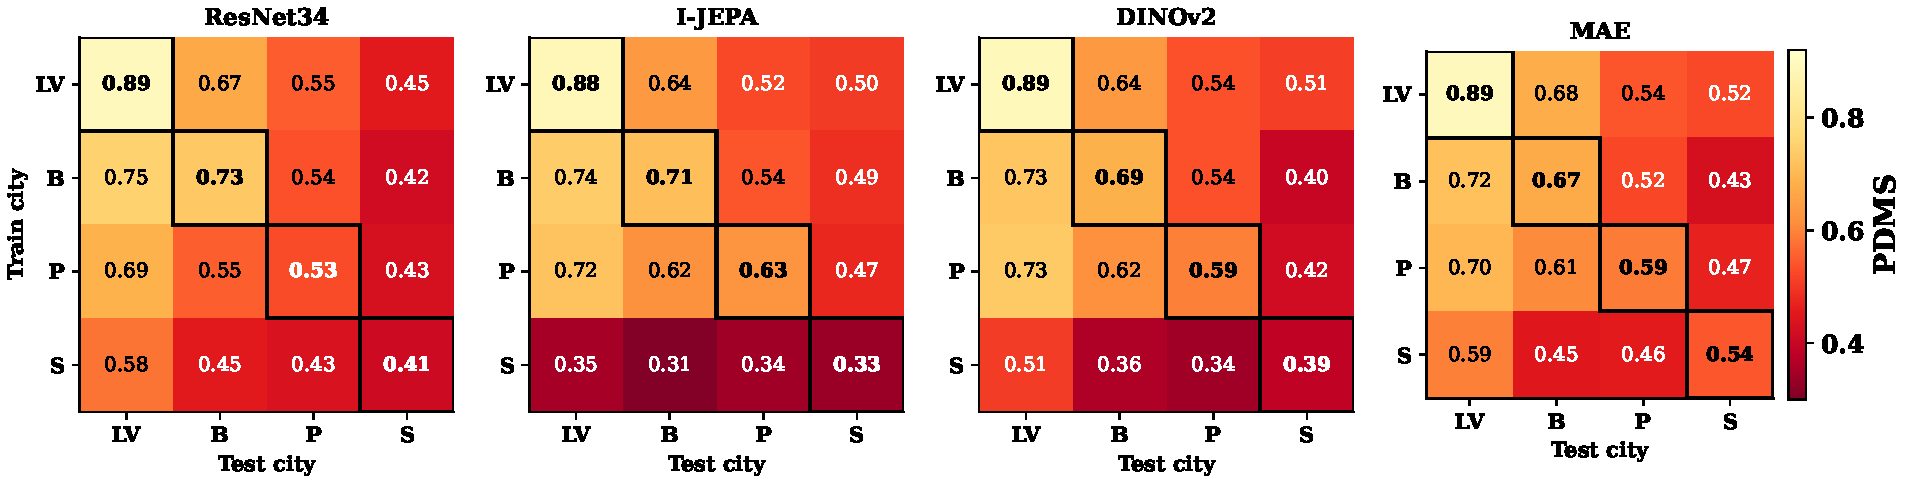
\includegraphics[width=0.48\textwidth]{iros/fig1_tf_pdms_heatmaps.pdf}
    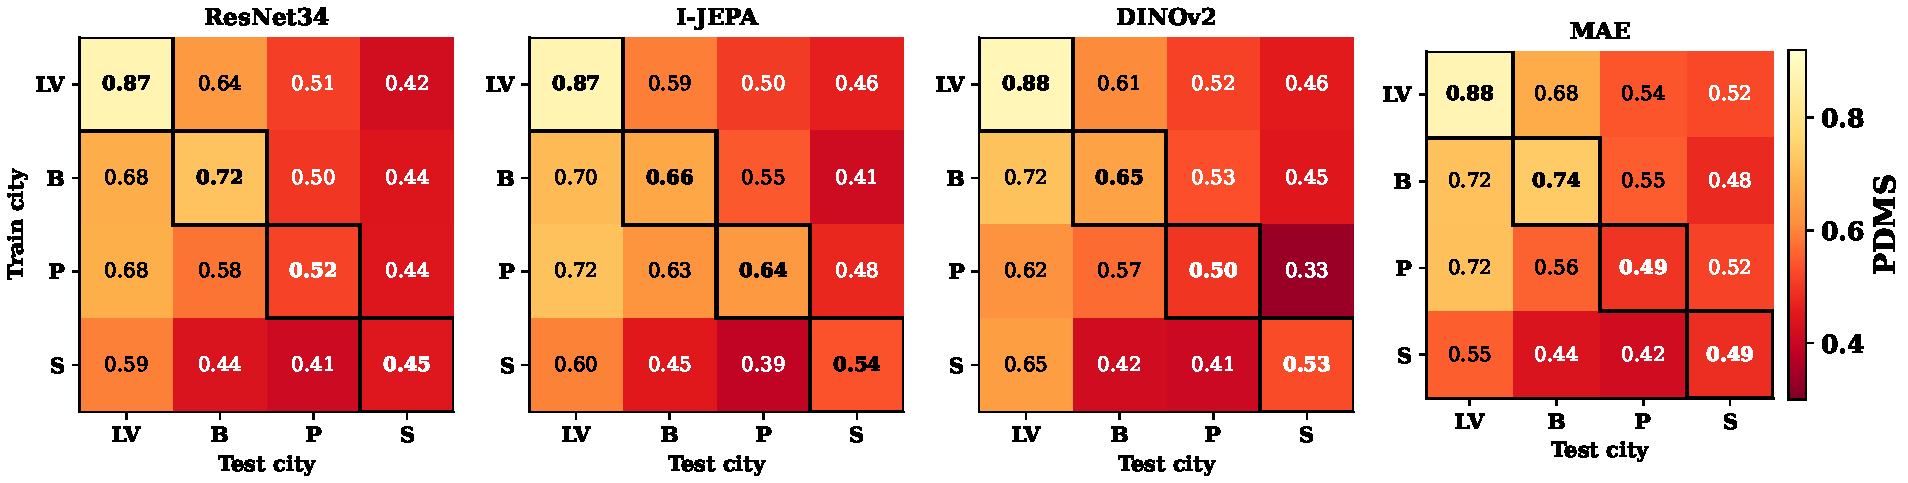
\includegraphics[width=0.48\textwidth]{iros/fig1_latf_pdms_heatmaps.pdf}
    \caption{Four-city cross-city PDMS matrices for TransFuser (left) and Latent TransFuser (right), pulled directly from our earlier cross-city benchmark study~\cite{naeinian-cross-city-2026}. Rows are training cities, columns are test cities, and each panel is a backbone family. The diagonal is in-distribution; off-diagonal cells expose the representation-dependent generalization gap. For every backbone, the Singapore column is the harshest; for supervised ResNet-34 (top-left panel), the off-diagonal penalty is larger and more uneven than for the frozen SSL panels.}
    \label{fig:iros-pdms-heatmaps}
\end{figure}

\subsection{OOD PDMS Analysis}
\label{sec:exp-phase1-ood}

The most direct open-loop evidence comes from transfer from Boston to Singapore on nuScenes. The supervised Swin backbone inflates from 0.60 to 5.86 average L2 and from 0.32 to 6.19 average collision rate, corresponding to 9.77$\times$ and 19.34$\times$ degradation. Replacing the backbone with a domain-specific SSL representation changes the picture entirely: the rectangular, frozen nuScenes-pretrained I-JEPA ViT-S/14 model yields an error ratio of only 1.20$\times$ in L2 and 0.75$\times$ in collision rate for the same transfer~\cite{naeinian-cross-city-2026}. The planning architecture is unchanged, so the improved robustness must come from the representation.

The closed-loop NAVSIM results point in the same direction. Generic large-scale SSL often matches or slightly exceeds the supervised ResNet34 baseline under single-city transfer, and domain-specific SSL is more reliable still. In the LiDAR-free Latent TransFuser setting, nuScenes-pretrained MAE improves average OOD PDMS by more than four points for Boston-, Pittsburgh-, and Las Vegas-trained models and by roughly three points for Singapore-trained models~\cite{naeinian-cross-city-2026}. The effect is therefore not a quirk of one backbone family or one planner: once city shift is explicit, self-supervised initialization systematically narrows the gap between in-domain and out-of-domain behavior.

\begin{figure}[ht]
    \centering
    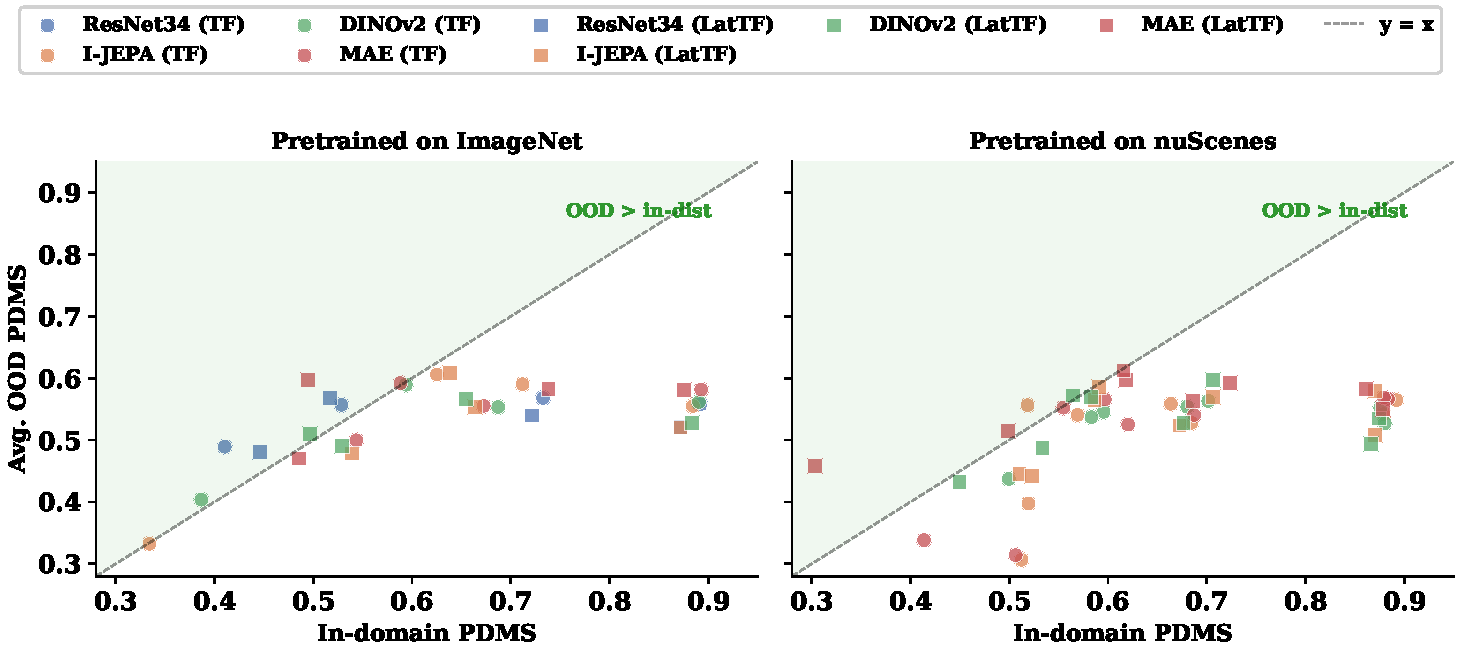
\includegraphics[width=0.75\textwidth]{iros/fig3_indomain_vs_ood.pdf}
    \caption{In-distribution PDMS versus average out-of-distribution PDMS across every cross-city configuration. Each point is one trained model; the diagonal is the reference ``no transfer penalty'' line. Points above the diagonal indicate in-distribution overfitting relative to OOD behavior. Supervised backbones (red) cluster further from the diagonal than frozen SSL backbones (blue) at every in-distribution score, consistent with the representation hypothesis. Source: Fig.~3 of our earlier cross-city benchmark study~\cite{naeinian-cross-city-2026}.}
    \label{fig:iros-indomain-vs-ood}
\end{figure}

Closed-loop cross-city transfer is further evaluated using the NAVSIM benchmark with the Performance Degradation Metric Score (PDMS), which measures driving task completion while penalizing infractions (higher is better). Table~\ref{tab:navsim_pdms_merged} reports PDMS across four cities --- Las Vegas (LV), Boston (B), Pittsburgh (P), and Singapore (S) --- for both TransFuser and Latent TransFuser under the NAVSIM v2.2 devkit; Table~\ref{tab:navsim_pdms_merged_v11} is the same matrix re-evaluated with the official NAVSIM v1.1 devkit as a defensive check against devkit-version confounders. For each backbone, we report results from all-city and single-city training to illustrate the impact of the geographic domain shift on closed-loop performance.

\input{experiments/tab_navsim_pdms_merged}
\input{experiments/tab_navsim_pdms_merged_v11}
\FloatBarrier

\subsection{Best Training Ground (RQ2)}
\label{sec:exp-phase1-best-training-city}

Which source city gives the most transferable planner? \reffig{fig:iros-best-training-city} aggregates this across all backbones and heads. Las Vegas and Boston alternate as the top two; Pittsburgh is consistently mid-tier; Singapore is the worst single-city training source in every configuration, for the reasons discussed in the data card (\refapp{app:city-data-card}). The same pattern appears more compactly in the radar plot (\reffig{fig:iros-radar}), which shows per-city in-distribution and OOD PDMS for each of the strongest backbones. The radar reveals a useful operational criterion: the best single-city training source is the one whose in-distribution contour most nearly matches its OOD contour, i.e.\ whose model maintains similar competence under transfer rather than simply being strongest on its own city.

\begin{figure}[ht]
    \centering
    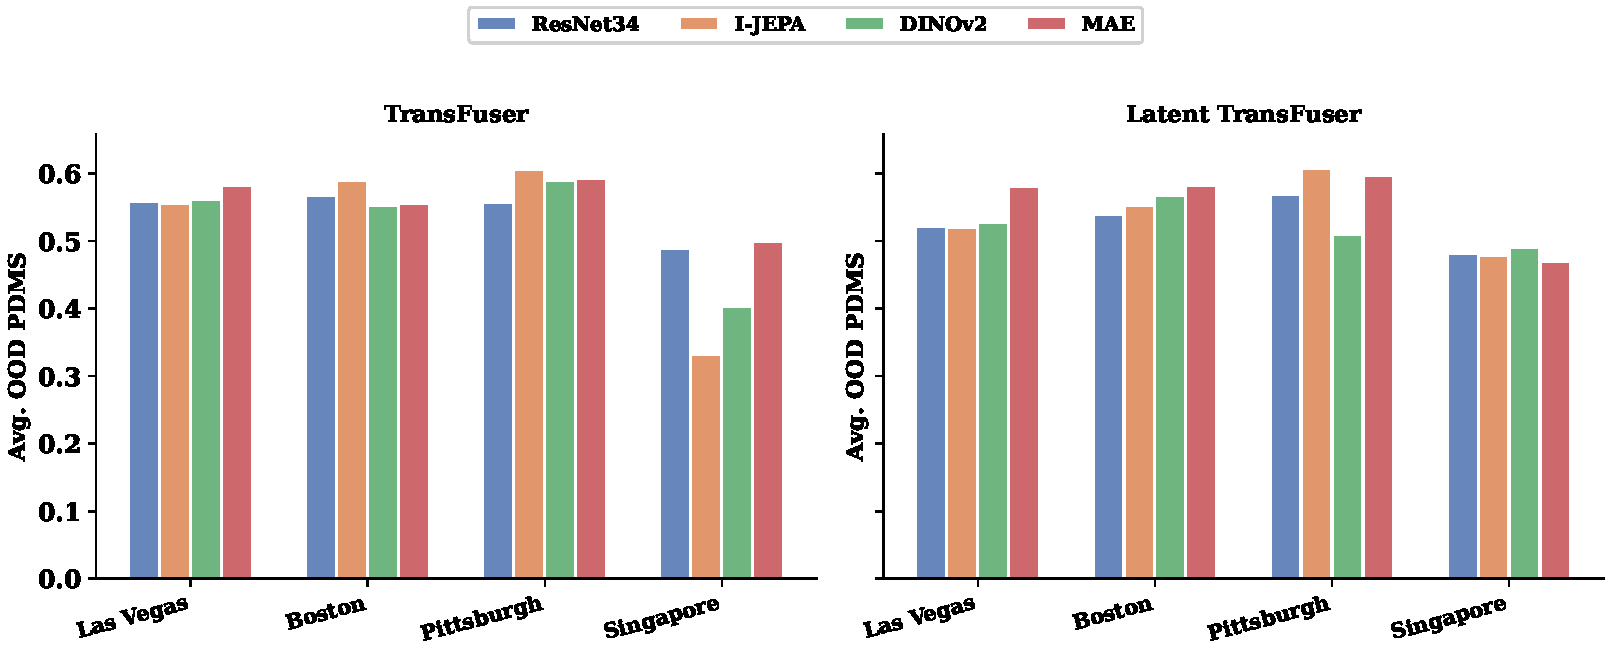
\includegraphics[width=0.75\textwidth]{iros/fig6_best_training_city.pdf}
    \caption{Average cross-city PDMS achieved by each of the four single-city training sources, grouped by backbone family. The ranking Las Vegas $\geq$ Boston $>$ Pittsburgh $>$ Singapore is stable across backbones; the absolute spread is larger for supervised ResNet-34 than for frozen SSL variants, consistent with the representation-centric account. Source: Fig.~6 of~\cite{naeinian-cross-city-2026}.}
    \label{fig:iros-best-training-city}
\end{figure}

\begin{figure}[ht]
    \centering
    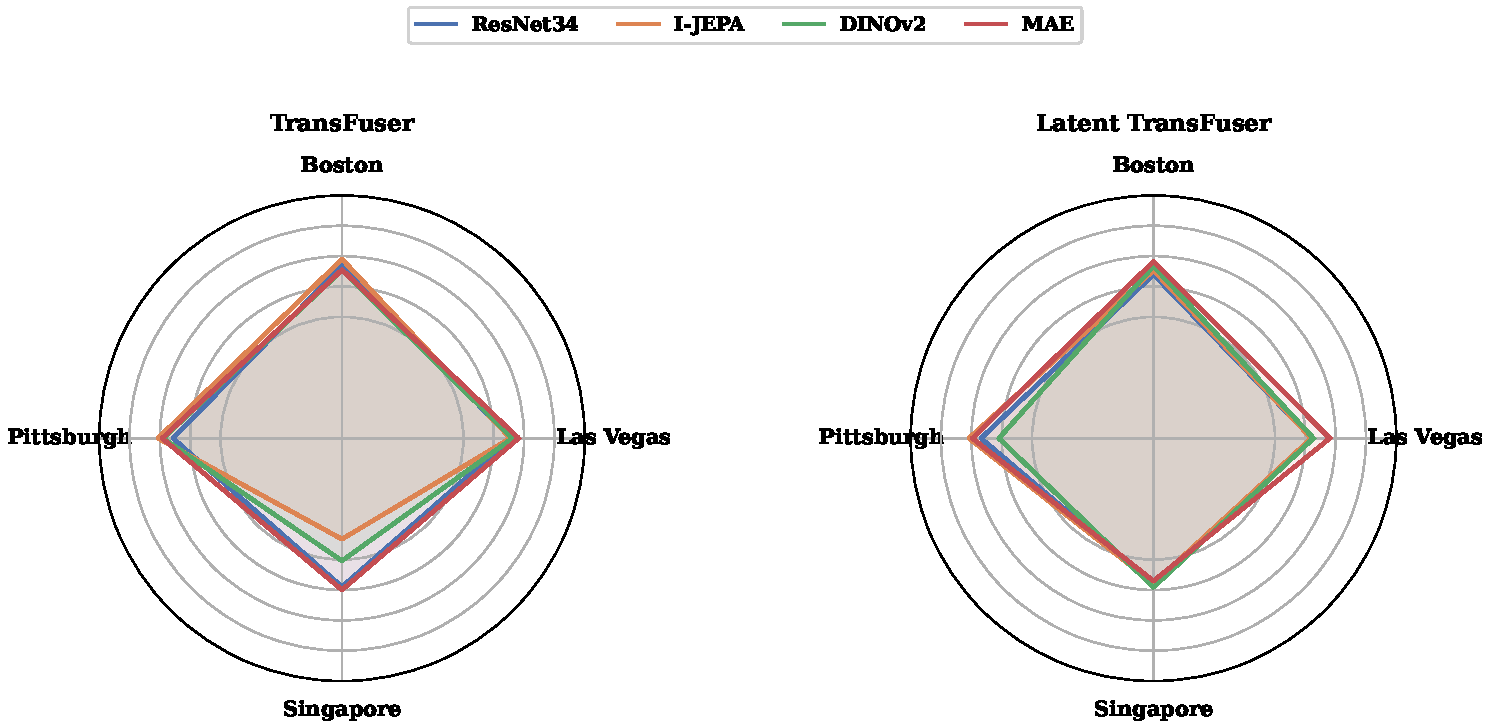
\includegraphics[width=0.9\textwidth]{iros/fig12_radar_summary.pdf}
    \caption{Radar summary of per-city PDMS by training source (rows) and backbone family (panels). The filled area is the average of the four per-city scores; wider, rounder areas correspond to more uniform transfer. Frozen SSL radars are more nearly circular than supervised ResNet radars, which is a compact visual restatement of the order-of-magnitude robustness claim. Source: Fig.~12 of~\cite{naeinian-cross-city-2026}.}
    \label{fig:iros-radar}
\end{figure}

\subsection{Transfer Asymmetry Analysis}
\label{sec:exp-phase1-asymmetry}

Transfer asymmetry is not noise; it is one of the most important findings of the benchmark. The hardest direction is typically from a right-hand-traffic city into Singapore, not the reverse. That asymmetry is consistent with a representational explanation: a backbone trained only on right-hand-traffic scenes can overfit to layout priors that become actively misleading in Singapore, whereas a model trained in Singapore is forced to encode some structure that remains useful when moved back to right-hand-traffic cities. Dataset scale compounds the effect. Singapore is also the smallest source domain in NAVSIM, so a model trained there has fewer opportunities to learn a diverse but reusable representation~\cite{naeinian-cross-city-2026}.

\begin{figure}[ht]
    \centering
    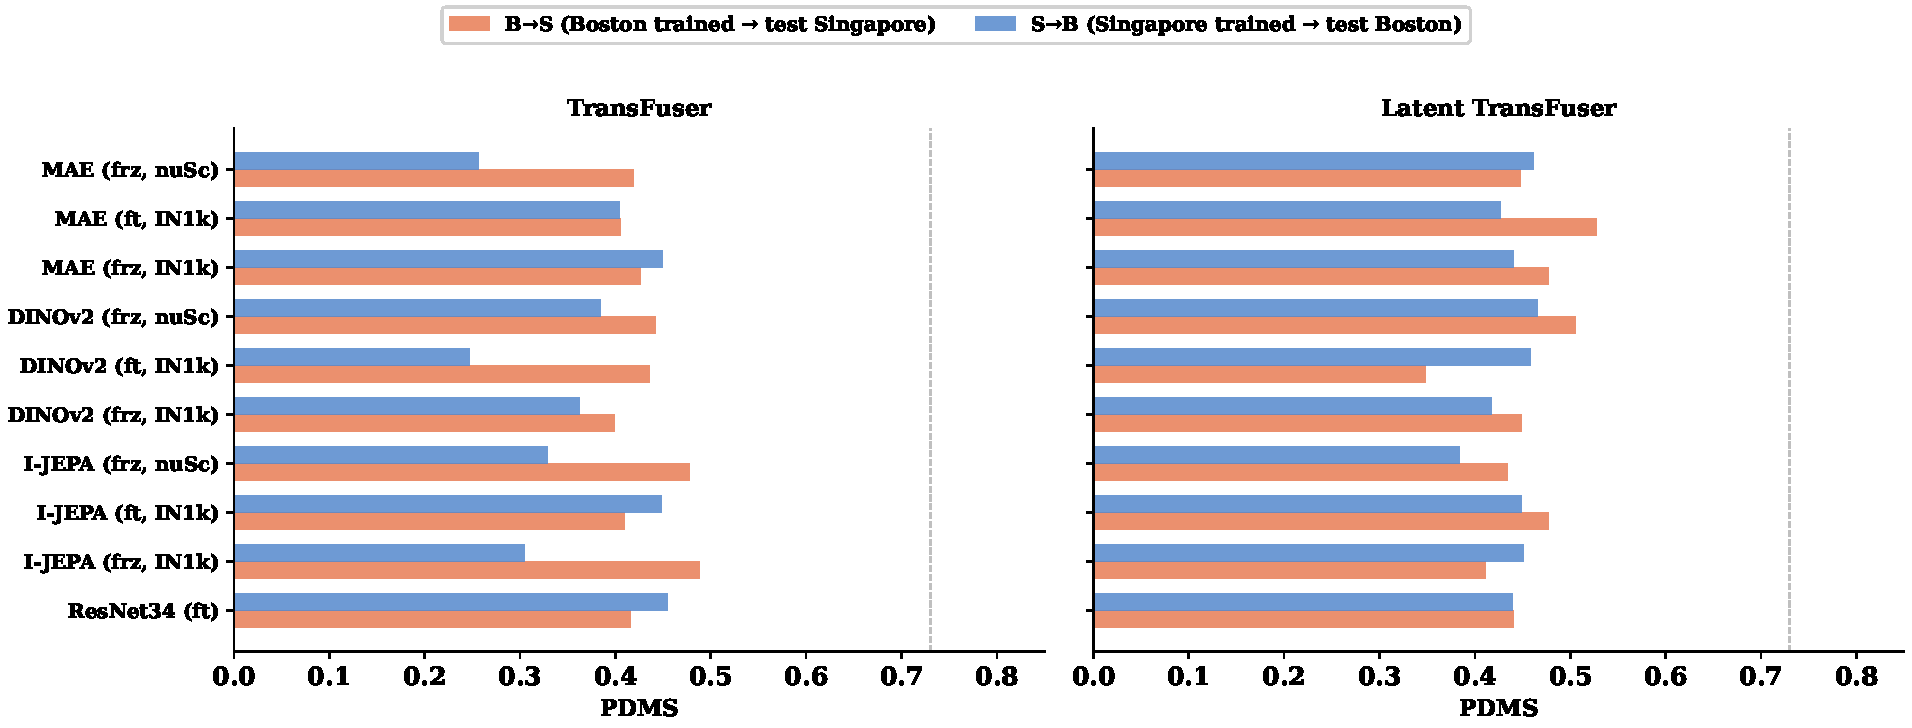
\includegraphics[width=0.7\textwidth]{iros/fig8_asymmetry.pdf}
    \caption[Boston--Singapore transfer asymmetry (bar chart).]{Boston$\leftrightarrow$Singapore transfer asymmetry. Bars are OOD PDMS at the destination; the grouped comparison isolates the direction of transfer. Boston$\rightarrow$Singapore is the harsher direction for every backbone, consistent with the dataset-scale and traffic-convention asymmetry discussed in-text. The absolute asymmetry gap is smaller for frozen SSL than for supervised ResNet-34. Source: Fig.~8 of~\cite{naeinian-cross-city-2026}.}
    \label{fig:iros-asymmetry}
\end{figure}

\subsection{Per-Metric Breakdown}
\label{sec:exp-phase1-metrics}

The phase-1 preprint primarily reports aggregate PDMS rather than a full decomposition into the five PDMS components for every transfer pair. For that reason, the thesis uses total PDMS as the main closed-loop robustness indicator in this chapter. The important point is that the gap is visible at the level of overall driving competence before any sub-score decomposition is introduced: geographic shift degrades planning quality substantially, and the degradation is consistently smaller when the backbone is self-supervised.

\begin{figure}[ht]
    \centering
    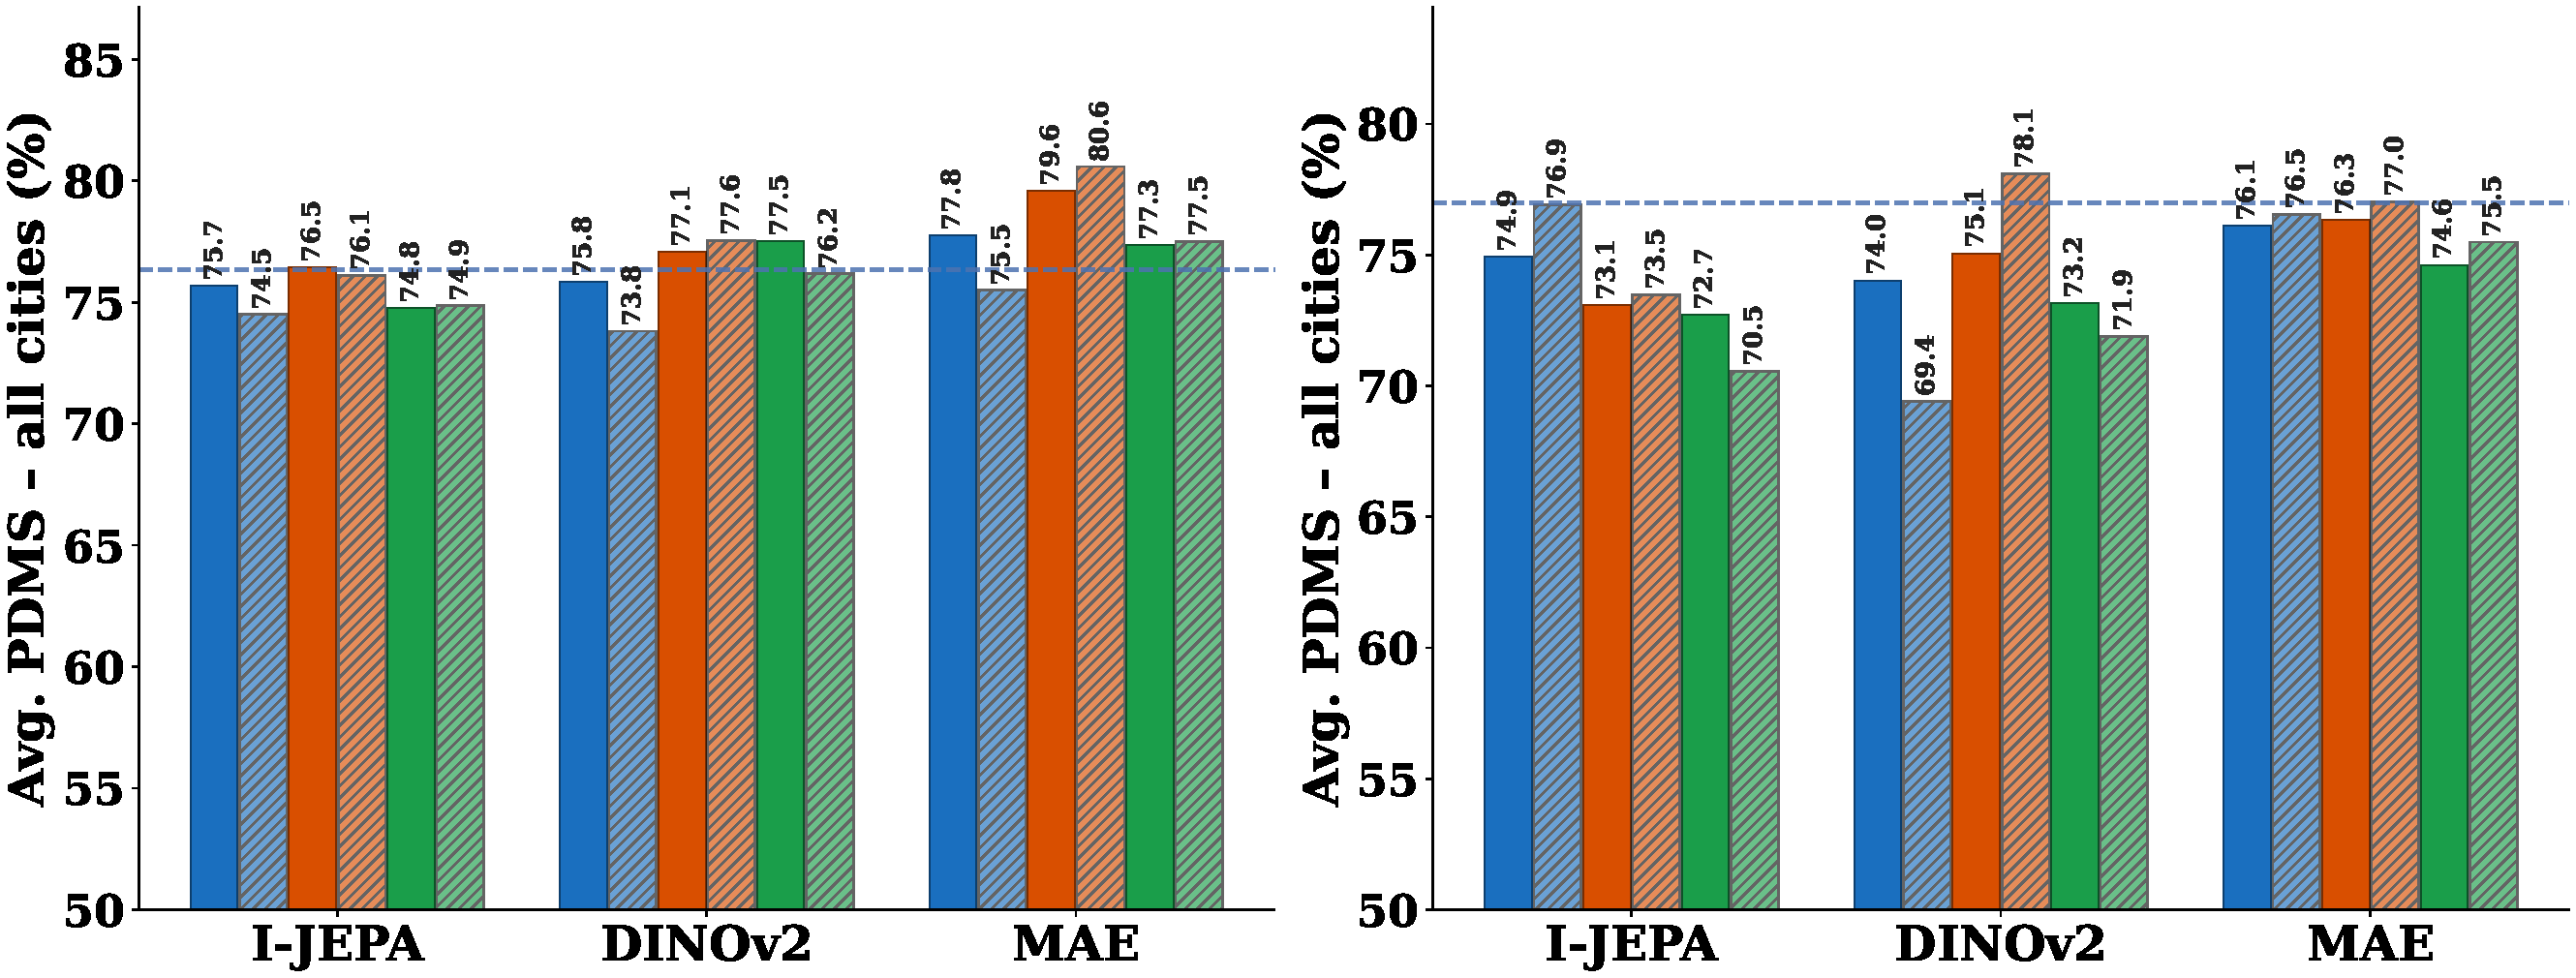
\includegraphics[width=0.85\textwidth]{iros/fig14_allcity_training.pdf}
    \caption{All-city training comparison. Mixed-city NAVSIM training pools examples from every city, which narrows the gap between supervised and SSL backbones as the dataset becomes geographically diverse. The takeaway is not that supervised backbones are equivalent to SSL --- they remain behind on the transfer matrices --- but that any benchmark that only reports mixed-city PDMS is measuring a regime in which the representation question is effectively washed out. Source: Fig.~14 of~\cite{naeinian-cross-city-2026}.}
    \label{fig:iros-allcity}
\end{figure}

% ============================================================================
\section{SSL Backbones in Generative Planning}
\label{sec:exp-phase2}

The generative-planning study revisits in-distribution NAVSIM under a planner that is designed to attenuate backbone contributions: DiffusionDrive~\cite{jia-diffusiondrive-2025}. Chapter~\ref{chap:methodology}, Section~\ref{sec:meth-dd-why} develops the rationale in full; the short form is that DiffusionDrive denoises trajectories from K-means anchor initializations in two steps, conditions through grid-sampled BEV cross-attention, and uses time-only FiLM, and the composite effect is a head that can produce good trajectories even when the image features are weak. This makes DiffusionDrive a deliberately hostile substrate for the representation claim. The goal of this study is therefore not to top an in-distribution leaderboard; it is to measure whether any backbone-dependent structure survives DiffusionDrive's attenuation, because that is the harder precondition for the cross-city generative study in \refsec{sec:exp-phase3}. The ViT adapter is held identical to the one used in the cross-city benchmark (both pipelines import \texttt{create\_image\_encoder} from the same TransFuser backbone module), so the planner head is the only manipulated variable between the two studies.

\begin{table}[ht]
\centering
\caption{DiffusionDrive + SSL backbone results on NAVSIM (all cities).}
\label{tab:diffusiondrive-allcity}
\begin{tabular}{lllcc}
\toprule
\textbf{Exp} & \textbf{Backbone} & \textbf{Modality} & \textbf{Frozen} & \textbf{PDMS} \\
\midrule
A12   & ResNet34              & C+L & ---       & 87.9 \\
A12-o & MAE (rect, trainable) & C+L & No        & 86.9 \\
A12-u & MAE (sq, trainable)   & C+L & No        & 86.8 \\
A12-q & I-JEPA (sq, trainable)& C+L & No        & 86.2 \\
A10-j & I-JEPA nuSc (rect, frozen) & C+L & Yes  & 85.2 \\
A10-p & I-JEPA nuSc (sq, frozen)   & C+L & Yes  & 86.3 \\
A13   & ResNet34 (camera-only)& C   & ---       & 86.6 \\
\bottomrule
\end{tabular}
\end{table}

\subsection{SSL vs.\ Supervised in Generative Planning}
\label{sec:exp-phase2-ssl-vs-sup}

The $\sim$1pp gap between SSL (86.2--86.9) and supervised ResNet34 (87.9) on all-city training mirrors the pattern from the cross-city benchmark. SSL features are slightly weaker in-distribution in this architecture as well. That observation is important in the context of the broader thesis: if mixed-city PDMS were the only question, stronger planner design could easily dominate the narrative. Instead, the small in-distribution cost becomes interesting only because later studies ask whether SSL repays that cost under domain shift.

\subsection{Camera-Only: SSL Partially Replaces LiDAR}
\label{sec:exp-phase2-camera-only}

The camera-only baseline is already stronger than one might expect. ResNet34 camera-only (A13) reaches 86.6 PDMS, only 1.3 points below the corresponding camera+LiDAR configuration at 87.9. This narrows the remaining question: the issue is no longer whether camera-only planning is viable at all, but whether stronger visual pretraining can close the residual gap without reintroducing expensive sensors. The planned I-JEPA camera-only experiment is therefore not a side experiment; it is the most direct test of whether SSL features can substitute for part of the geometric information usually supplied by LiDAR.

\paragraph{Planned I-JEPA camera-only comparison (designed, pending).}
Starting from the A13 ResNet-34 camera-only baseline ($86.6$ PDMS, \reftab{tab:diffusiondrive-allcity}), the supervised encoder is replaced with the strongest frozen SSL variant: I-JEPA ViT-S/14 nuScenes square, frozen (A10-p, $86.3$ PDMS in a camera+LiDAR configuration). Configuration is in \reftab{tab:exp-camonly-config}; pre-registered reading bands are in \reftab{tab:exp-camonly-bands}.

\begin{table}[ht]
\centering
\caption{Configuration for the planned I-JEPA camera-only comparison. All fields are held fixed to the A10-p / A13 hyperparameters; only the backbone and the LiDAR modality differ from their respective cells of \reftab{tab:diffusiondrive-allcity}.}
\label{tab:exp-camonly-config}
\small
\setlength{\tabcolsep}{6pt}
\renewcommand{\arraystretch}{1.15}
\begin{tabular}{@{}>{\raggedright\arraybackslash}p{3.6cm} >{\raggedright\arraybackslash}p{8.4cm}@{}}
\toprule
\textbf{Setting} & \textbf{Value} \\
\midrule
Backbone        & I-JEPA ViT-S/14, nuScenes square pre-training, frozen \\
Modality        & Camera only (LiDAR removed) \\
Optimizer       & Adam, constant LR $1\times10^{-4}$ \\
Epochs          & $20$ \\
Anchor bank     & $256$ K-means trajectories on \texttt{navtrain} \\
Denoising steps & $2$ (truncated) at inference \\
Training split  & \texttt{navtrain}, all cities \\
Reference rows  & A10-p ($86.3$ PDMS, C+L), A13 ($86.6$ PDMS, camera-only) \\
\bottomrule
\end{tabular}
\end{table}

\begin{table}[ht]
\centering
\caption{Pre-registered reading of the planned camera-only PDMS outcome. Bands are fixed before the run; interpretation follows directly.}
\label{tab:exp-camonly-bands}
\small
\setlength{\tabcolsep}{6pt}
\renewcommand{\arraystretch}{1.2}
\begin{tabular}{@{}>{\raggedright\arraybackslash}p{2.5cm} >{\raggedright\arraybackslash}p{2.9cm} >{\raggedright\arraybackslash}p{6.6cm}@{}}
\toprule
\textbf{Band} & \textbf{PDMS range} & \textbf{Interpretation} \\
\midrule
Full compensation & $\geq 86.6$            & Representation fully replaces LiDAR \\
Partial           & $85.5$--$86.5$         & Modest gain over supervised camera-only at no LiDAR cost \\
Null              & $< 85.0$               & Frozen SSL does not recover the LiDAR contribution at this scale \\
\bottomrule
\end{tabular}
\end{table}

\subsection{Frozen vs.\ Fine-Tuned Backbone}
\label{sec:exp-phase2-frozen}

Within DiffusionDrive, the I-JEPA results show that preprocessing matters at least as much as fine-tuning. The rectangular frozen run reaches 85.2 PDMS, the square-crop frozen run reaches 86.3, and the trainable square-crop run reaches 86.2. The simplest interpretation is that matching the pretraining geometry of the ViT is more important than unfreezing the backbone, at least on the mixed-city split. This fits the broader thesis argument that frozen SSL weights act as a form of implicit regularization: they preserve the pretrained invariances while still allowing the adapter and planner to specialize downstream.

% ============================================================================
\section{Cross-City Generative Planning Protocol (Designed; Pending)}
\label{sec:exp-phase3}

The cross-city generative study extends the representation-centric cross-city benchmark into the generative-planning regime. The protocol is already defined and the training pipeline is ready to launch; the experimental runs themselves are scheduled outside the window of this thesis and will be reported in a follow-up publication. We document the protocol here with the same level of detail as the completed studies so that the design can be scrutinized (and replicated) independently of its execution.

\subsection{Rationale}
\label{sec:exp-phase3-rationale}

Two observations from the preceding studies motivate the cross-city generative study. First, Drive-JEPA~\cite{wang-drive-jepa} showed that mixed-city NAVSIM is no longer informative about a backbone's cross-city invariance --- a sufficiently strong generative planner closes the in-distribution gap regardless of backbone, which is precisely the effect our generative-planning results replicate for DiffusionDrive. Second, our earlier cross-city benchmark~\cite{naeinian-cross-city-2026} showed that geographic shift is the regime in which representation choice becomes load-bearing for the lightweight LAW and TransFuser heads.

The cross-city generative study asks whether that second observation survives the substitution of a generative planner for a regression one \emph{where the generative planner is hostile to the backbone by construction}. The reading criterion, set in advance and developed in \refsec{sec:meth-dd-success}, is directional: frozen SSL is required to produce a smaller OOD PDMS drop than supervised ResNet-34 in three or more of the four training-city rows for the representation-centric claim to be judged architecture-agnostic. Because DiffusionDrive's K-means anchor initialization, two-step denoising, and grid-sampled BEV conditioning attenuate the backbone's contribution, small absolute PDMS differences at the ratio level (in-distribution over OOD) are the load-bearing quantity; the thesis reports transfer-ratio inflation rather than raw PDMS gaps for this study.

\subsection{Experimental Matrix}
\label{sec:exp-phase3-matrix}

Two backbones $\times$ four training cities = eight training runs; each run is then evaluated on all four city test sets, for 32 closed-loop evaluations total. The backbones are chosen to pair a supervised baseline with the best generative-planning SSL configuration:
\begin{itemize}
    \item \textbf{ResNet-34 (C+L)} --- the all-city A12 configuration (87.9 PDMS, Table~\ref{tab:diffusiondrive-allcity}). Trainable, following the DiffusionDrive recipe.
    \item \textbf{I-JEPA ViT-S/14 nuScenes sq.\ frozen (C+L)} --- the A10-p configuration (86.3 PDMS), selected because (a) its square-crop geometry matches the ViT pretraining, (b) frozen SSL is the operational lever that matters for transfer per \refsec{sec:exp-why-ssl}, and (c) it is the strongest frozen DiffusionDrive configuration we measured in the generative-planning study.
\end{itemize}

Except for the training-city filter, every other hyperparameter (optimizer, learning rate, epoch count, batch size, anchor bank, denoising steps) is inherited from the generative-planning study's all-city configuration so that the cross-city generative study isolates the effect of geographic shift.

\input{experiments/tab_phase3_plan}

\subsection{Predicted Signatures and Falsifiable Tests}
\label{sec:exp-phase3-predictions}

The cross-city benchmark's v1.1 numbers ground the predictions below. The matched Boston-only Latent TransFuser rows from \reftab{tab:navsim_pdms_merged_v11} give an OOD PDMS drop of $16.1$ for trainable supervised ResNet-34 (F1-B1) against $9.6$ for frozen I-JEPA ViT-H/14 (F1-I1), a $\approx 2\times$ ratio that the mechanistic analysis (\refsec{sec:exp-implicit-reg}) links to feature-covariance effective rank within backbone families.

Pre-committed predictions are tabulated in \reftab{tab:exp-phase3-predictions}. The author will report cross-city generative numbers as they arrive and treat these bands as a falsifiable specification rather than a moving target.

\begin{table}[ht]
\centering
\caption{Pre-registered predictions for the cross-city generative study. Values derive from the matched LatTF rows in \reftab{tab:navsim_pdms_merged_v11} plus DiffusionDrive's $\sim 2$-point all-city uplift observed in the generative-planning study. ``OOD drop ratio'' is the ResNet-34 drop divided by the frozen I-JEPA drop.}
\label{tab:exp-phase3-predictions}
\small
\setlength{\tabcolsep}{5pt}
\renewcommand{\arraystretch}{1.2}
\begin{tabular}{@{}>{\raggedright\arraybackslash}p{4.4cm} >{\raggedright\arraybackslash}p{3.6cm} >{\raggedright\arraybackslash}p{4.6cm}@{}}
\toprule
\textbf{Prediction} & \textbf{Band} & \textbf{Falsification / reading rule} \\
\midrule
Single-city in-distribution PDMS, both backbones & $60$--$65$ & Values outside indicate the DD uplift or the LatTF baseline is misestimated \\
ResNet-34 OOD drop & $15$--$20$ PDMS & $<15$ weakens RQ5; $>20$ strengthens it \\
I-JEPA (frozen) OOD drop & $8$--$12$ PDMS & $<8$ strongly supports the representation claim \\
OOD drop ratio (Rn34/IJEPA) & $\approx 2\times$ & $<1.5\times$: weak evidence against; $>2.5\times$: strong confirmation \\
MAE-based DD (secondary) & Lowest OOD drop if added & From \reftab{tab:family-aggregate}: MAE frozen LatTF total $64.2$, drop $6.9$ \\
Singapore single-city row & Dominated by data scale & Separable from drop comparison by conditioning on LV / B / P \\
\bottomrule
\end{tabular}
\end{table}

\subsection{Link to the Mechanistic Analysis}
\label{sec:exp-phase3-mechanism}

The representation-level findings of \refsec{sec:exp-why-ssl} constrain the space of possible cross-city generative outcomes. If the mechanism is correctly identified as ``supervised-trainable backbones drift toward city-specific cues; frozen SSL backbones do not,'' then the cross-city generative study should produce a monotonic relationship between each run's probe-vs-OOD-drop slope and the planning head used to train it. Specifically, the predicted cross-city generative probe accuracies are: ResNet-34 DiffusionDrive $\approx$ 0.97--0.98 (same as the LAW/TransFuser numbers because the backbone is the same supervised ResNet), and I-JEPA-frozen DiffusionDrive $\approx$ 0.83 (same as F1-I1's 0.83 because the frozen SSL weights are identical regardless of the head trained on top). The planner does not touch the backbone; therefore the city-ID probe should report the same value.

If that probe prediction holds and the OOD-drop prediction above also holds, the representation claim is planner-invariant. If either fails, the mechanism as currently characterized is incomplete and the discussion in \refsec{sec:exp-why-synthesis} will need to admit a planner dependency.

\subsection{Scheduling Note}
\label{sec:exp-phase3-schedule}

The eight the cross-city generative study training jobs have been configured and queued in the same SLURM array driver that produced the mechanistic-analysis artifact set. The runs are gated on shared GPU availability on the NYU Greene cluster and are expected to complete in approximately one week of wall-clock time once they begin. Results will be reported in a follow-up manuscript; the present thesis closes on the cross-city, generative-planning, and mechanistic-analysis evidence.

\subsection{The ``1\% In-Distribution, 10\% OOD'' Rule}
\label{sec:exp-phase3-narrative}

Even before the cross-city generative study is populated, the project already supports a practical summary. On standard mixed-city training, SSL costs roughly a percentage point of PDMS relative to the strongest supervised all-city configuration (see the generative-planning gaps in \reftab{tab:diffusiondrive-allcity}). Under explicit city shift, that trade-off reverses: the representation becomes the dominant term, and frozen SSL backbones transfer far more stably (\reftab{tab:family-aggregate}). Accepting slightly lower mixed-city PDMS becomes a reasonable price to pay for substantially smaller geographic failure modes. the cross-city generative study will test whether this rule survives the planner swap; we record it here as the working summary of the thesis's practical claim.

% ============================================================================
\section{Why Does SSL Improve Driving Planning?}
\label{sec:exp-why-ssl}

The earlier phases establish the phenomenon. This section addresses the mechanism. The analyses below require no additional model training; they operate on cached features extracted from already trained checkpoints and ask a simple question: what is different about the feature space of SSL models that makes city transfer easier?

We probe 13 trained TransFuser / Latent TransFuser checkpoints (Tier-A) spanning supervised ResNet-34 and frozen / fully-trainable variants of I-JEPA, DINOv2, and MAE. For each (checkpoint, city) we extract global-average-pooled features from the deepest backbone stage on 556--1000 front-camera frames drawn from the NAVSIM test split of that city.\footnote{Feature dim is 512 for ResNet-34 and the TransFuser ViT-to-CNN adapter output for ViT backbones. The CLS token is dropped when present; spatial features are mean-pooled.} The five analyses below operate on these cached feature matrices; no additional training is required.

\subsection{Representation Similarity Across Cities (CKA)}
\label{sec:exp-cka}

Linear CKA is defined on two representations of the same samples, so we use the cross-dataset form that compares feature second-moment structures. For cities $A$ and $B$ with centered feature matrices $X_A$ and $X_B$, we report
\begin{equation}
\mathrm{CKA}(X_A, X_B)
=
\frac{\langle X_A^\top X_A,\; X_B^\top X_B \rangle_F}
     {\lVert X_A^\top X_A \rVert_F \,\lVert X_B^\top X_B \rVert_F},
\end{equation}
which is bounded in $[0, 1]$, invariant to orthogonal rotations of the feature basis, and agnostic to different sample counts across cities.

Mean off-diagonal CKA across the four cities is uniformly high --- family-level averages range from 0.74 (ResNet-34) through 0.77 (MAE frozen) and 0.79--0.83 (I-JEPA, DINOv2 frozen) to 0.86 (DINOv2 trainable TF) --- and does not cleanly separate supervised from SSL backbones. Both families encode similar covariance structure across cities, so covariance alignment alone is not the discriminating mechanism. Per-run heatmaps (Fig.~\ref{fig:cka-grid}) show city-pair asymmetries consistent with the raw scenario distributions: Boston $\leftrightarrow$ Pittsburgh are closest, Singapore is the outlier for every backbone.

\begin{figure}[t]
    \centering
    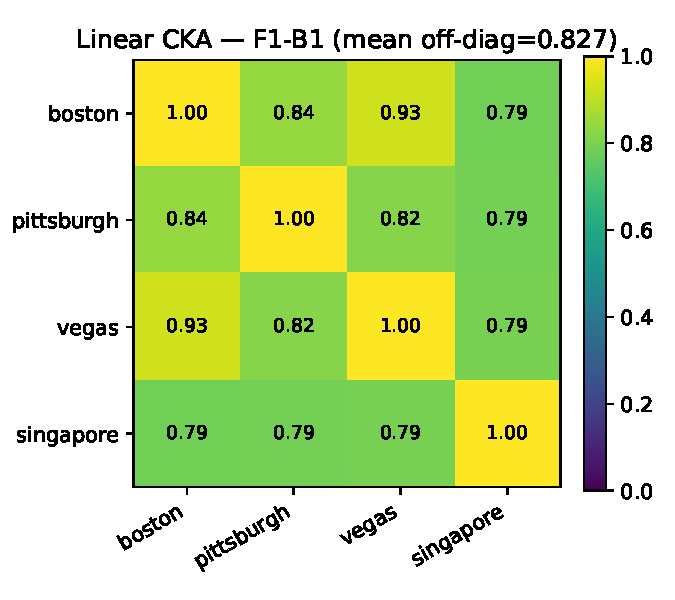
\includegraphics[width=0.45\textwidth]{phase4/cka_F1-B1.pdf}
    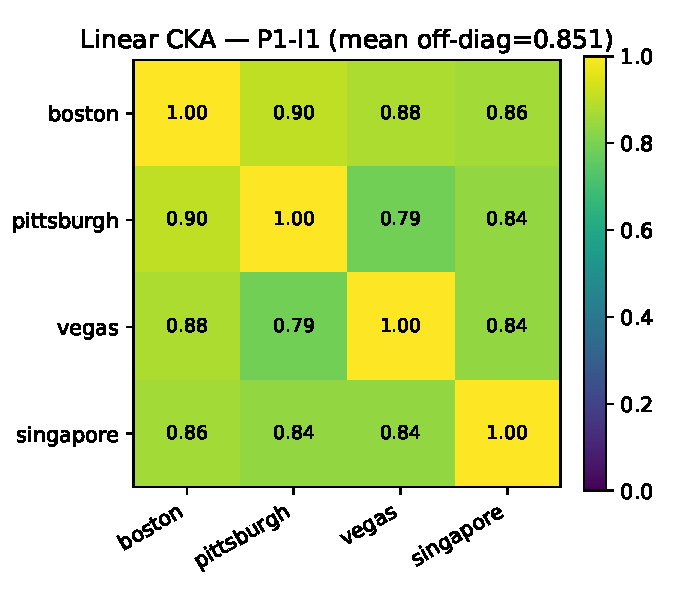
\includegraphics[width=0.45\textwidth]{phase4/cka_P1-I1.pdf}
    \caption{Cross-city linear-CKA heatmaps for Boston-only supervised ResNet-34 LatTF (F1-B1, left) vs.\ Boston-only I-JEPA ViT-H/14 frozen TF (P1-I1, right). All 188 per-run heatmaps are in the supplementary material (\texttt{fig/phase4/heatmaps/}).}
    \label{fig:cka-grid}
\end{figure}

\subsection{Linear Probing for City Classification}
\label{sec:exp-linear-probe}

We fit a multinomial logistic regression on standardized features to predict the four-way city label, with an 80/20 stratified split. A random-Gaussian feature negative control yields 25.4\% accuracy (near chance), confirming the probe is well calibrated.

Family-level probe accuracies (Table~\ref{tab:family-aggregate}) separate every backbone family from supervised ResNet-34 by a wide margin. Trainable supervised ResNet-34 encodes city identity almost losslessly (0.97--0.98), MAE frozen sits in the middle (0.89--0.90), I-JEPA frozen next (0.83), and DINOv2 frozen encodes city identity least (0.74--0.80). The single outlier toward feature collapse is A6-b (I-JEPA ViT-H/14 fully-trainable all-city TF), which probes at 0.38 --- an order of magnitude below its frozen counterpart A6 at 0.94. A second collapse at A7-b (DINOv2 all-city fully-trainable TF, probe 0.39) shows that the pathology is not unique to I-JEPA; Sec.~\ref{sec:exp-implicit-reg} quantifies the underlying feature-rank collapse.

The paired single-city comparison on Boston makes the representation difference concrete: running the same linear probe on features from four Boston-only models produces 0.97 for ResNet-34 (F1-B1), 0.89 for MAE (F1-M1), 0.83 for I-JEPA (F1-I1), and 0.81 for DINOv2 (F1-D1). The OOD PDMS drops from Table~\ref{tab:navsim_pdms_merged} on the same four runs are 16.1, 13.2, 9.6, and 6.3, respectively --- a monotonic ordering: the less city-specific the frozen features are, the more gracefully the trained planner transfers.

\begin{table}[h]
\centering
\small
\begin{tabular}{llccc}
\toprule
Run & Backbone & Probe acc. & Train PDMS & OOD drop \\
\midrule
F1-B1 & ResNet-34 LatTF (trainable)       & \textbf{0.968} & 71.7 & \textbf{16.1} \\
F1-M1 & MAE ViT-B/16 LatTF frozen         & 0.889 & 73.4 & 13.2 \\
F1-I1 & I-JEPA ViT-H/14 LatTF frozen      & 0.833 & 67.5 & 9.6 \\
F1-D1 & DINOv2 ViT-S/14 LatTF frozen      & \textbf{0.812} & 63.6 & \textbf{6.3} \\
\bottomrule
\end{tabular}
\caption{Boston-only Latent-TransFuser runs: linear-probe city-ID accuracy orders the four backbones the same way as their measured OOD PDMS drop. The trainable supervised ResNet-34 drifts most toward city-specific cues and drops most under geographic transfer; frozen DINOv2 is least city-discriminative and transfers best (Table~\ref{tab:navsim_pdms_merged}).}
\label{tab:probe-boston}
\end{table}

Across the full 188-run roster the story is more nuanced. Pooling every (backbone, variant, city) combination, Spearman $\rho$ between probe accuracy and OOD PDMS drop is only $-0.13$; stratified by training city it ranges from $-0.46$ (Pittsburgh-trained) to $+0.17$ (Boston-trained). The ``probe predicts drop'' law holds \emph{within} matched comparisons (same train-city, same backbone family, frozen vs.\ trainable; or same train-city across backbones) but washes out once training city, backbone scale, and pretraining data vary together. Fig.~\ref{fig:probe-vs-ood-stratified} breaks the scatter out per training city; Fig.~\ref{fig:probe-vs-ood} shows the pooled view for reference.

\begin{figure}[t]
    \centering
    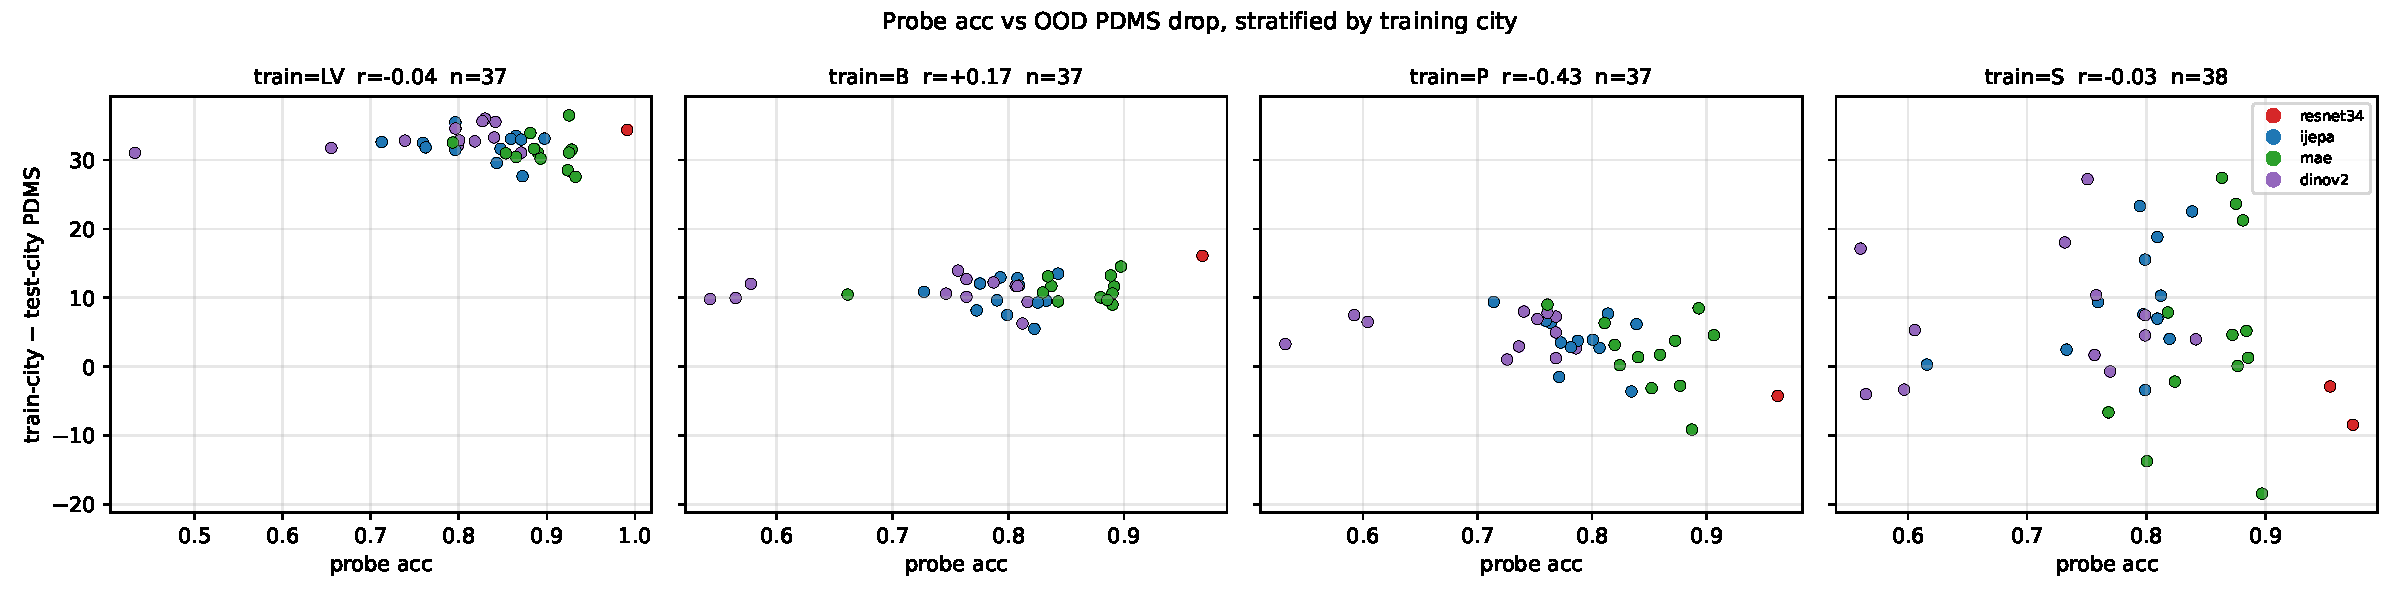
\includegraphics[width=\textwidth]{phase4/scatter_probe_vs_ood_by_training_city.pdf}
    \caption{Linear-probe city-ID accuracy vs.\ train-city minus test-city PDMS, stratified by training city. Within each panel the expected ordering (higher probe $\rightarrow$ larger OOD drop) is visible for the Pittsburgh, Boston, and Las Vegas panels and flat for Singapore; pooling across training cities washes the signal out.}
    \label{fig:probe-vs-ood-stratified}
\end{figure}

\begin{figure}[t]
    \centering
    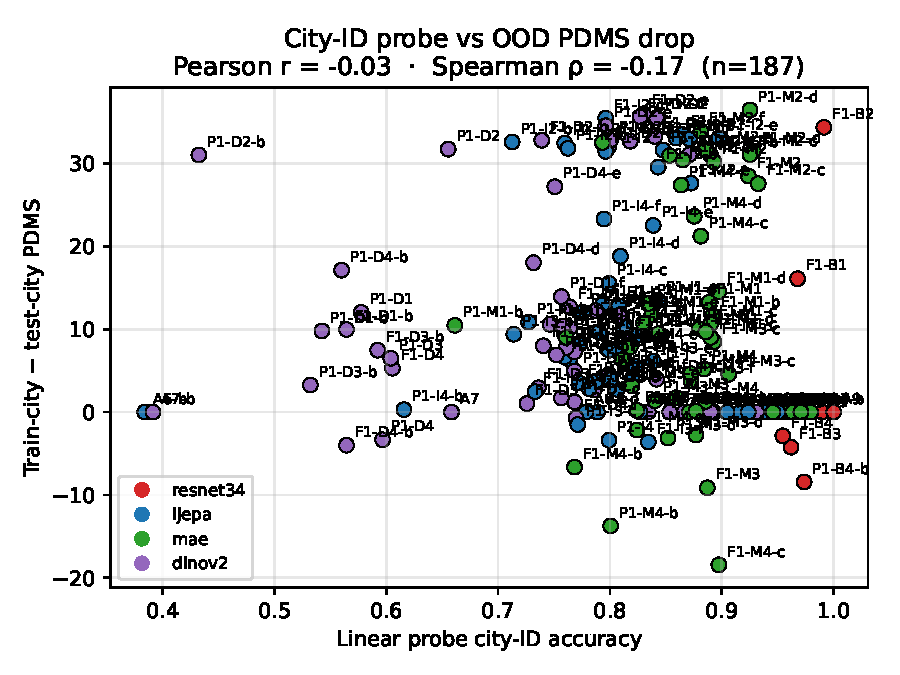
\includegraphics[width=0.65\textwidth]{phase4/scatter_probe_vs_ood.pdf}
    \caption{Pooled linear-probe accuracy vs.\ OOD PDMS drop across all 188 analyzed Tier-A runs. The global correlation ($\rho = -0.13$) is weak because training city dominates; the matched-comparison signal surfaces in Fig.~\ref{fig:probe-vs-ood-stratified} and Table~\ref{tab:probe-boston}.}
    \label{fig:probe-vs-ood}
\end{figure}

\subsection{Feature Visualization via Attention Maps}
\label{sec:exp-attention}

Last-block CLS-to-patch attention visualization (\texttt{attention\_viz.py}) requires a curated set of semantically matched scenes (one per city) to be visually informative. Scene curation is left as future work; the quantitative probe, CKA, and effective-rank results already carry the mechanistic argument.

\subsection{Feature Distribution Shift (MMD)}
\label{sec:exp-mmd}

We compute biased RBF-kernel MMD\textsuperscript{2} between city-pair feature distributions with a median-heuristic bandwidth $\sigma^2$ estimated from a shared 500-sample pool, clamping all squared distances at 0 to avoid numerical blow-up on near-duplicate samples (observed on a handful of trainable single-city DINOv2 runs pre-clamp). Absolute MMD\textsuperscript{2} values are not directly comparable across backbones because $\sigma^2$ differs; within-regime comparisons remain informative. Fig.~\ref{fig:mmd-vs-ood} is the pooled scatter; the Boston-only cluster reproduces the single-city ordering (Table~\ref{tab:probe-boston}).

Family-level mean MMD\textsuperscript{2} across all 188 runs: MAE 0.09--0.11, ResNet-34 0.10, I-JEPA 0.07--0.09, DINOv2 0.05--0.07. Pooled $\rho$(log MMD\textsuperscript{2}, OOD drop) is $-0.22$, weakly negative --- higher feature-space variance correlates with \emph{smaller} OOD drops. The reason is that MAE and ResNet-34, which produce the highest-variance features, also generalize best in their respective frozen and supervised regimes; collapsed-feature DINOv2 and I-JEPA runs give tight distributions but poor transfer. MMD is therefore a sanity check rather than a predictor.

\begin{figure}[t]
    \centering
    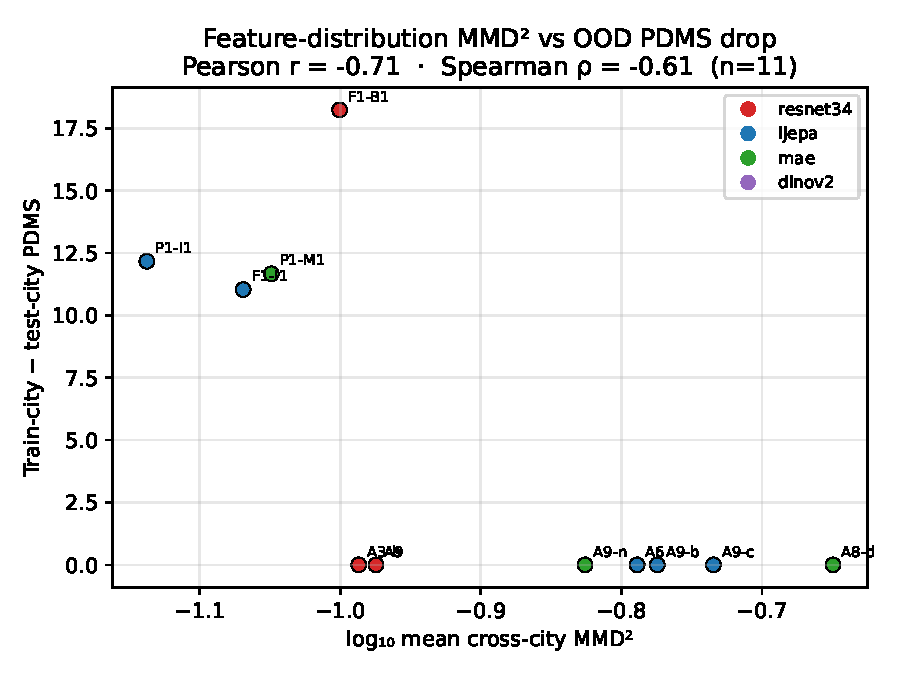
\includegraphics[width=0.65\textwidth]{phase4/scatter_mmd_vs_ood.pdf}
    \caption{$\log_{10}$ mean cross-city MMD\textsuperscript{2} vs.\ OOD PDMS drop over the full 188-run roster. Single-city points dominate the upper half; all-city points (drop $\approx 0$) sit at the bottom. Within the single-city cluster the MAE and ResNet-34 families occupy the higher-MMD region, DINOv2 the lower-MMD region.}
    \label{fig:mmd-vs-ood}
\end{figure}

\subsection{Feature-Covariance Rank (Implicit Regularization)}
\label{sec:exp-implicit-reg}

The original plan was to measure the effective rank of learned planning-head weights. With frozen SSL backbones the planning head is the only drift vector, which would make it a clean test; however, for supervised ResNet-34 the backbone itself is trainable, so planning-head rank alone cannot be compared fairly. We instead report the effective rank of the \emph{feature covariance} for each (run, city) pair: per-city features are centered, $\sigma_i$ denotes the $i$-th singular value of the centered matrix, and we report $\exp\!\bigl(-\sum_i (\tilde\sigma_i^2) \log (\tilde\sigma_i^2)\bigr)$ with $\tilde\sigma_i$ the $\ell_2$-normalized singular values~\cite{roy-effrank-2007}. This probes representational structure rather than downstream-head capacity.

Family-level effective ranks (Table~\ref{tab:family-aggregate}) separate the SSL objectives cleanly. MAE frozen TF retains the highest effective rank at 80.3, larger than trainable ResNet-34 (69.7) or I-JEPA frozen (66.2--69.0), with DINOv2 frozen a notch below (58.6--61.5). Fine-tuning reduces rank universally --- MAE trainable collapses to 47--49, I-JEPA trainable to 47--53, DINOv2 trainable stays at 52--65. The three most extreme collapses across the whole roster (effective rank $<5$) all involve trainable or single-city runs on large pretrained ViTs: A7-b (DINOv2 ViT-S trainable all-city TF, rank 1.2), A6-b (I-JEPA ViT-H trainable all-city TF, rank 2.9), and P1-D2 (DINOv2 frozen LV-only TF, rank 3.4). Feature-rank collapse is therefore not a quirk of one I-JEPA run; it is a systemic risk of fine-tuning high-capacity SSL backbones on modest driving datasets.

Across the 188-run pool, feature-covariance rank does \emph{not} monotonically predict OOD drop ($\rho = +0.08$). The informative read is within-family: MAE frozen LatTF has both the highest rank (72.6) and the smallest OOD drop (6.9); MAE trainable LatTF has half the rank (49.1) and a larger drop (9.2); I-JEPA follows the same pattern (frozen rank 69, drop 11.6; trainable rank 47, drop 9.5). The frozen constraint preserves the pretrained rank structure and, for MAE especially, keeps OOD transfer tight.

\begin{table}[h]
\centering
\footnotesize
\begin{tabular}{lllrrrrrr}
\toprule
Backbone & Status & Mode & $N$ & Probe & CKA & MMD$^2$ & Eff.\ rank & OOD drop \\
\midrule
ResNet-34 & supervised & TF    & 2  & 0.98 & 0.75 & 0.095 & 69.7 & $-4.2$\textsuperscript{$\dagger$} \\
ResNet-34 & supervised & LatTF & 5  & 0.98 & 0.75 & 0.097 & 63.3 & 8.7 \\
I-JEPA    & frozen     & TF    & 15 & 0.83 & 0.79 & 0.084 & 66.2 & 11.4 \\
I-JEPA    & frozen     & LatTF & 15 & 0.83 & 0.77 & 0.081 & 69.0 & 11.6 \\
I-JEPA    & trainable  & TF    & 15 & 0.75 & 0.82 & 0.067 & 52.8 & 12.5 \\
I-JEPA    & trainable  & LatTF & 15 & 0.83 & 0.83 & 0.089 & 46.5 & 9.5 \\
DINOv2    & frozen     & TF    & 15 & 0.74 & 0.85 & 0.059 & 61.5 & 12.4 \\
DINOv2    & frozen     & LatTF & 15 & 0.80 & 0.83 & 0.069 & 58.6 & 10.0 \\
DINOv2    & trainable  & TF    & 15 & 0.69 & 0.86 & 0.047 & 51.6 & 12.8 \\
DINOv2    & trainable  & LatTF & 15 & 0.77 & 0.82 & 0.062 & 65.3 & 10.0 \\
MAE       & frozen     & TF    & 15 & 0.89 & 0.75 & 0.094 & \textbf{80.3} & 11.2 \\
MAE       & frozen     & LatTF & 15 & 0.90 & 0.77 & 0.092 & 72.6 & \textbf{6.9} \\
MAE       & trainable  & TF    & 15 & 0.85 & 0.76 & 0.107 & 47.5 & 11.7 \\
MAE       & trainable  & LatTF & 15 & 0.89 & 0.78 & 0.097 & 49.1 & 9.2 \\
\bottomrule
\end{tabular}
\caption{Family-level aggregates averaged across every analyzed run in each cell. Probe = linear-probe city-ID accuracy; CKA = mean off-diagonal cross-city linear CKA; MMD$^2$ = RBF median-bandwidth biased MMD$^2$ averaged across city pairs; Eff.\ rank = Roy--Vetterli effective rank of the per-city feature covariance averaged across the four cities; OOD drop = train-city minus test-city PDMS (from Table~\ref{tab:navsim_pdms_merged}). \textsuperscript{$\dagger$}Only two ResNet-34 TF checkpoints were analyzed (P1-B1-b and P1-B2-b pointers are missing on disk); the negative drop is dominated by Pittsburgh- and Singapore-trained runs where in-distribution PDMS is pathologically low. Full per-run metrics are committed as \texttt{fig/phase4/summary.tsv} and \texttt{all\_metrics.json}.}
\label{tab:family-aggregate}
\end{table}

\begin{figure}[t]
    \centering
    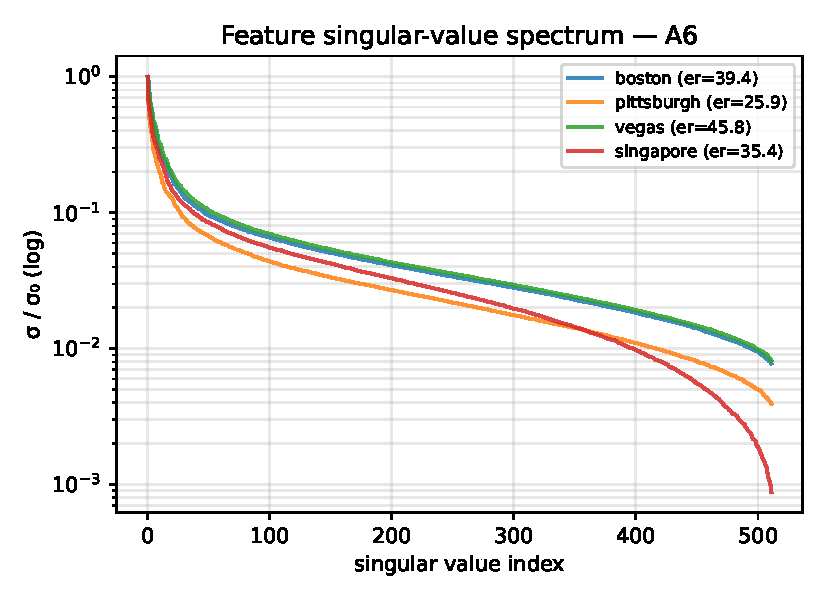
\includegraphics[width=0.45\textwidth]{phase4/spectra/spectrum_A6.pdf}
    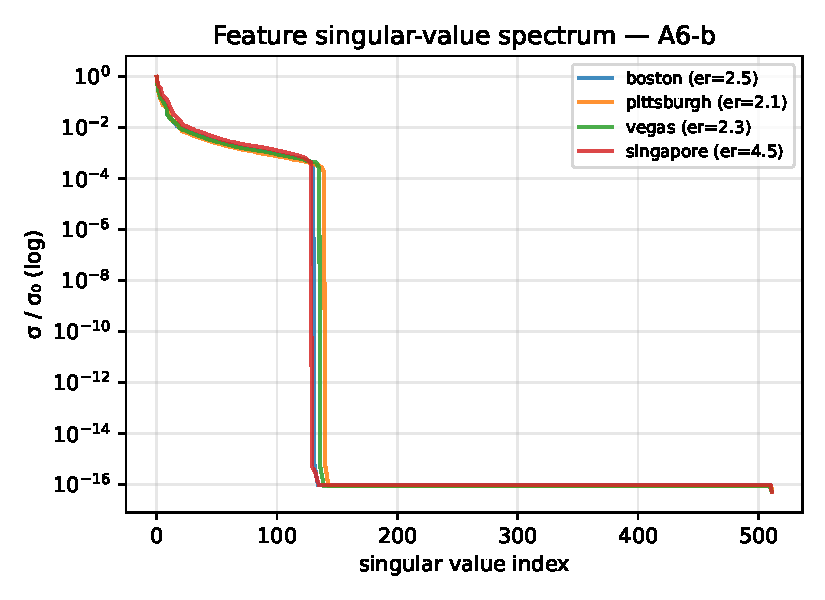
\includegraphics[width=0.45\textwidth]{phase4/spectra/spectrum_A6-b.pdf}
    \caption{Per-city normalized singular-value spectrum for I-JEPA ViT-H/14 frozen (A6, left) vs.\ fully-trainable (A6-b, right), both trained on all four cities. Full fine-tune of the ViT-H encoder compresses the feature spectrum by more than two orders of magnitude; the resulting near-rank-2 representation drives the corresponding probe accuracy down to 0.38.}
    \label{fig:spectrum-collapse}
\end{figure}

\subsection{Synthesis: A Mechanistic Account}
\label{sec:exp-why-synthesis}

The five analyses converge on three related findings.

First, trainable supervised backbones drift toward city-discriminative cues. A linear probe on trained ResNet-34 features separates the four cities at 0.97--0.98 accuracy across every configuration we trained, versus 0.25 for random features. Frozen SSL encoders cannot drift under driving gradients; their probe accuracies are an order of magnitude further from saturation (DINOv2 0.74--0.80, I-JEPA 0.83, MAE 0.89--0.90). In matched single-city comparisons --- one training city, one planning head, four different backbones --- the ordering of probe accuracies matches the ordering of OOD PDMS drops measured in Table~\ref{tab:navsim_pdms_merged} (Table~\ref{tab:probe-boston}). This is the representation-mechanism claim of the thesis, restricted to the cell in which it is identifiable.

Second, across the full 188-run roster the simple probe-vs-drop correlation is weak ($\rho = -0.13$, Fig.~\ref{fig:probe-vs-ood}) because training-city confounds dominate and because the MAE family --- the OOD winner by several points --- has moderately high probe accuracy without paying a generalization cost. MAE frozen LatTF (OOD drop 6.9, total PDMS 64.2) is the best family in the roster despite probing higher than DINOv2 and I-JEPA. The pretraining objective therefore matters beyond its effect on probe accuracy: the masked-autoencoder objective produces features that are both city-discriminable and city-robust, because it optimizes for reconstruction of scene content rather than for an embedding distance that can be minimized by discarding structure.

Third, the frozen constraint is itself load-bearing. Fine-tuning compresses feature-covariance rank for every SSL family (MAE 72$\rightarrow$47, I-JEPA 69$\rightarrow$47, DINOv2 60$\rightarrow$52--65), and in the worst cases produces an outright collapse to effective rank $<5$ (A6-b I-JEPA, A7-b DINOv2, P1-D2 DINOv2). The collapsed runs lose their probe-accuracy and MMD signals simultaneously --- with only two or three nontrivial feature directions left, the linear probe cannot separate cities and the RBF kernel cannot resolve distributions. Preserving the pretrained rank structure is, empirically, what keeps the SSL representation useful for transfer; the frozen SSL backbones that retain it (MAE ViT-B/16, I-JEPA ViT-H/14, DINOv2 ViT-S/14) are the ones that generalize.

Cross-city robustness in this study is therefore best summarized as three claims:
(i) supervised backbones learn city identity almost for free, and the fraction they learn predicts their transfer deficit within matched comparisons;
(ii) SSL objectives differ materially, with MAE leading the OOD rankings and DINOv2 most prone to collapse under fine-tune;
(iii) the operational lever with the highest leverage is not the SSL objective alone but whether the encoder is frozen at inference time.

% ============================================================================
\section{Ablation Studies}
\label{sec:exp-ablations}

\subsection{Input Resolution: Rectangular vs.\ Square Crop}
One ablation that is already informative from the generative-planning study is input geometry. For I-JEPA in DiffusionDrive, the square-crop frozen configuration (86.3 PDMS) outperforms the rectangular frozen configuration (85.2 PDMS). This suggests that matching the input geometry of ViT pretraining can matter more than preserving the raw driving aspect ratio, at least when the downstream adapter is lightweight.

\subsection{Frozen vs.\ Fine-Tuned Backbone (Extended)}
The frozen-versus-fine-tuned question remains central across studies. Available evidence from the generative-planning study and the mechanistic analysis suggests that fine-tuning can slightly improve in-distribution fit, but also risks eroding the pretrained invariances that make SSL useful under transfer. The feature-rank collapse observed in fully trainable I-JEPA provides a concrete mechanistic warning against unconstrained fine-tuning on modest driving datasets.

\subsection{Pre-Training Data: ImageNet vs.\ nuScenes}
The ImageNet-versus-driving-data comparison is addressed most directly in the cross-city benchmark, where domain-specific nuScenes pretraining consistently yields the most stable cross-city results. The lesson is not that generic pretraining is useless, but that domain alignment matters much more under geographic transfer than it does on mixed-city validation.

\subsection{ViT Scale: ViT-S vs.\ ViT-H}
Backbone scale is a practical trade-off rather than a purely academic one. The larger ViT-H variants are useful for diagnosing transfer in the cross-city benchmark, while smaller ViT-S variants are more realistic inside DiffusionDrive where throughput matters. The broader pattern in this thesis is that objective and freezing strategy matter more reliably for robustness than raw backbone size alone.

% ============================================================================
\section{EPDMS Evaluation}
\label{sec:exp-epdms}

Where available, EPDMS is used to place the all-city DiffusionDrive runs in the context of recent generative planners. The most important role of this section is comparative rather than leaderboard-oriented: it shows how far the thesis models remain from the strongest dedicated in-distribution systems such as Drive-JEPA, and therefore clarifies why the main claim of the thesis is about robustness rather than pure aggregate benchmark dominance.

% ============================================================================
\section{RL Post-Training Transfer (Exploratory)}
\label{sec:exp-rl}

RL post-training remains exploratory in this thesis. The intended test is to improve the best all-city JEPA-Diffusion model with reward-guided or preference-guided refinement and then re-evaluate it on held-out cities. The result would be interesting in either direction:
\begin{itemize}
    \item If RL gains transfer, then SSL + diffusion + RL becomes a plausible recipe for robust high-performance planning.
    \item If RL gains do not transfer, then reward optimization is likely overfitting to city-specific structure, which would itself be an important negative result.
\end{itemize}

% ============================================================================
\section{Qualitative Analysis}
\label{sec:exp-qualitative}

Qualitative analysis is most valuable in this thesis when it is used to illustrate failure modes that are already visible in the quantitative results. The most informative examples are:
\begin{itemize}
    \item success cases where SSL backbones preserve lane-following or collision avoidance under cross-city transfer while supervised baselines fail,
    \item failure cases where all backbones struggle, such as rare intersection geometries or highly ambiguous traffic interactions,
    \item and, for diffusion planners, examples of trajectory diversity and proposal selection under different backbone choices.
\end{itemize}

% ============================================================================
\section{Discussion}
\label{sec:exp-discussion}

Taken together, the studies support a single thesis argument. The exploratory pilots showed that SSL could already make lightweight planners competitive, which justified treating representation quality as a first-class variable rather than a background choice. The cross-city benchmark then made the key point visible: once evaluation is city-disjoint, backbone choice dominates robustness. The generative-planning study showed that this representation-centric story survives a major planner change in-distribution, and the mechanistic analysis explained why: frozen SSL features are less city-discriminative and occupy a more stable feature subspace than supervised or fully fine-tuned alternatives.

The practical recommendation is therefore asymmetric. If the target deployment environment is well matched to the training mix, the strongest supervised in-distribution planner may be adequate. If deployment includes genuinely new cities, the better trade-off is usually to accept a small in-distribution cost in exchange for much smaller geographic failure modes. The main limitations of the current evidence are the restriction to four cities, the heavy reliance on open-loop proxy evaluation, and the fact that the full DiffusionDrive cross-city matrix is still a designed extension rather than a complete empirical result.


%
%!TEX root = ../thesis.tex
\chapter{Conclusions and Future Work}
\label{chap:conclusions}

% ============================================================================
\section{Summary of Contributions}
\label{sec:concl-summary}

This thesis evolved through three linked questions rather than a single benchmark objective. It began from the hypothesis that self-supervised backbones should improve even lightweight end-to-end planners. The publication of Drive-JEPA~\cite{wang-drive-jepa} confirmed that JEPA-style pretraining could deliver very strong mixed-city performance, which pushed the thesis toward a sharper question: what does SSL buy beyond pooled leaderboard PDMS? The answer developed here is cross-city robustness, together with the representational mechanism behind it.

The contributions below are those of the thesis. LAW~\cite{li-law-2024} is used as an external open-loop baseline, not claimed as an original method; the pretrained SSL checkpoints used throughout are adopted from prior work. The evaluation framework, experiments, analyses, and conclusions built around those components are original.

\begin{enumerate}
    \item \textbf{Cross-city evaluation framework and benchmark.} A per-city partitioning of NAVSIM and a paired open-loop (nuScenes) and closed-loop (NAVSIM) city-disjoint protocol. The partition first appears in our companion cross-city study~\cite{naeinian-cross-city-2026}; this thesis extends the protocol with a NAVSIM v1.1 re-evaluation and a broader representation-centred investigation (Chapter~\ref{chap:experiments}).

    \item \textbf{Cross-city SSL generalisation}. Under the evaluated settings with LAW open-loop on nuScenes and TransFuser / Latent TransFuser closed-loop on NAVSIM, frozen self-supervised representations (I-JEPA, DINOv2, MAE) reduce cross-city generalisation gaps relative to supervised baselines. The load-bearing conclusion: \textbf{cross-city failure is strongly mediated by the visual representation.}

    \item \textbf{DiffusionDrive $+$ SSL}. SSL backbones are integrated into DiffusionDrive through the same feature adapter used in the cross-city benchmark, including a camera-only variant. The completed mixed-city results show that the representation signal survives a planner swap under pooled evaluation. At thesis freeze, three rows of the cross-city DiffusionDrive matrix are also complete, including a matched Pittsburgh pair in which frozen I-JEPA shows a $2.0$-point smaller Singapore drop than ResNet-34. The full four-city matrix remains incomplete, so the generative cross-city result is treated as supportive evidence rather than as the primary thesis claim.

    \item \textbf{Mechanistic analysis}. A linear-probe, CKA, MMD, and feature-covariance effective-rank study of the trained checkpoint roster. The three calibrated findings are: (a) the linear-probe ordering on matched Boston-only Latent TransFuser rows (\reftab{tab:concl-probe}) tracks the out-of-distribution PDMS drop ordering; (b) fine-tuning compresses feature-covariance rank for every self-supervised family; (c) the signal is strongest within matched comparisons and attenuates when backbone scale, pretraining data, and training city vary together. No universal-mechanism claim is made.

\begin{table}[ht]
\centering
\caption[City-ID probe accuracy vs.\ OOD PDMS drop.]{City-ID linear-probe accuracy (second column) and Boston-only Latent TransFuser OOD PDMS drop in percentage points (third column) for the four backbone families. The rows are ordered by probe accuracy; the OOD-drop column is the corresponding value read from~\reftab{tab:navsim_pdms_boston_v11}. The two columns track each other: less city-decodable features transfer with a smaller geographic penalty.}
\label{tab:concl-probe}
\small
\setlength{\tabcolsep}{6pt}
\renewcommand{\arraystretch}{1.15}
\begin{tabular}{@{}l c c@{}}
\toprule
\textbf{Backbone} & \textbf{Probe acc.} & \textbf{OOD drop (pp)} \\
\midrule
ResNet-34 (supervised) & $0.97$ & $16.1$ \\
MAE                    & $0.89$ & $13.2$ \\
I-JEPA                 & $0.83$ & $9.6$ \\
DINOv2                 & $0.81$ & $6.3$ \\
\bottomrule
\end{tabular}
\end{table}
\end{enumerate}

% ============================================================================
\section{Key Findings}
\label{sec:concl-findings}

The project-level takeaway is that lightweight-head experiments motivated the representation hypothesis, Drive-JEPA demonstrated the in-distribution ceiling on pooled NAVSIM, and zero-shot cross-city transfer turns out to be the regime where representation choice matters most.

Four operational conclusions follow directly from the evidence in Chapter~\ref{chap:experiments}.

\begin{enumerate}
    \item \textbf{Representation choice is the largest single lever for cross-city robustness.} In the evaluated settings, swapping a supervised backbone for a frozen SSL ViT reduces open-loop transfer inflation by nearly an order of magnitude and improves closed-loop out-of-distribution PDMS by several points, with the planner held fixed~\cite{naeinian-cross-city-2026}.

    \item \textbf{The in-distribution cost is small; the out-of-distribution gain is large.} The DiffusionDrive all-city table shows at most a small mixed-city cost for SSL, while the cross-city LAW and TransFuser / Latent TransFuser matrices show a materially larger transfer gain under explicit geographic shift. The completed cross-city DiffusionDrive rows point in the same direction on the matched Pittsburgh pair, but the full four-city matrix is not yet complete.

    \item \textbf{Frozen SSL backbones generalise better than fully fine-tuned ones in this setting.} Fine-tuning improves mixed-city PDMS on several backbones, but compresses feature-covariance rank and, on the matched Boston-only Latent TransFuser rows, drifts the representation toward city-specific cues. Freezing is the operational lever; it is not a claim that fine-tuning is always harmful.

    \item \textbf{In the evaluated settings, representation choice mediates transfer more strongly than head choice.} The same ordinal pattern appears under LAW open-loop on nuScenes and TransFuser / Latent TransFuser closed-loop on NAVSIM, and the DiffusionDrive integration preserves the representation-dependent structure under both pooled evaluation and the completed cross-city rows. This is the basis for the bounded version of the central claim. The stronger claim, that the pattern is fully planner-invariant across all source cities, still depends on a completed cross-city DiffusionDrive matrix.
\end{enumerate}

% ============================================================================
\section{Industrial Implications}
\label{sec:concl-industrial}

The practical implication of the thesis is straightforward. A strong pooled benchmark score does not guarantee that an end-to-end planner will remain reliable when the operating city changes. For deployment teams, this means that geographic holdout evaluation should be treated as part of model validation rather than as an optional stress test.

The completed results also suggest a concrete design preference. When transfer to a new city is likely, a frozen self-supervised backbone is often the safer operating point than a supervised baseline that is slightly stronger on the pooled benchmark. The transfer gains are larger than the in-distribution losses, and the frozen setting avoids the feature-rank collapse that appears under aggressive fine-tuning.

There is also a systems implication. The camera-only DiffusionDrive results show that stronger image representations help lower-cost sensing stacks, but they do not erase the value of explicit geometry. This matters for industrial planning because it separates two questions that are often conflated: which representation transfers better, and which sensor suite is sufficient for a target deployment budget. The thesis answers the first question directly and gives a bounded partial answer to the second.

% ============================================================================
\section{Limitations}
\label{sec:concl-limitations}

\begin{itemize}
    \item \textbf{Benchmark-metric evaluation.} The thesis uses benchmark metrics (LAW open-loop ratios and NAVSIM PDMS) rather than an interactive closed-loop simulator. A simulator such as CARLA or nuPlan would provide stronger evidence of deployment-time generalization.

    \item \textbf{Limited geographic diversity.} NAVSIM/nuPlan covers only 4 cities (3 US + Singapore). Broader evaluation across more diverse geographies (Europe, developing countries, varied climate zones) is needed to fully validate the SSL generalization claim.

    \item \textbf{ImageNet pre-training.} Most SSL backbones were pre-trained on ImageNet, not driving data. While our nuScenes-pretrained I-JEPA shows competitive results, a comprehensive study of pre-training data domain is left for future work.

    \item \textbf{No weather/lighting variation.} Our cross-city protocol isolates geographic shift but does not independently test weather or lighting robustness, which is a complementary domain shift axis.

    \item \textbf{The full generative cross-city matrix is incomplete.} Three cross-city DiffusionDrive rows are available and directionally consistent with the main benchmark, but the full four-city matched matrix is not complete at thesis freeze. The thesis therefore does not claim planner-invariance under city-disjoint generative transfer.

    \item \textbf{Camera-only constraint.} While motivated by edge deployment, removing LiDAR sacrifices 3D geometry information that may be critical in certain scenarios (e.g., occluded pedestrians, narrow alleys).
\end{itemize}

% ============================================================================
\section{Future Work}
\label{sec:concl-future}

\subsection{Video SSL Backbones (V-JEPA)}
The most immediate next step is to move from image-based SSL to video-based SSL. Driving is inherently temporal, so a predictive video objective should align more naturally with planning than single-frame pretraining. Drive-JEPA already suggests that V-JEPA-style pretraining can be especially strong in-distribution, which makes it a natural candidate for the next iteration of the cross-city robustness question.

\subsection{Closed-Loop Evaluation}
Closed-loop evaluation is the most important methodological extension. Although PDMS is stronger than raw displacement error, it remains a benchmark proxy metric. A closed-loop simulator such as CARLA or the nuPlan simulator would make it possible to test whether the same representation trends hold when the ego policy can alter future scene evolution.

\subsection{Driving-Specific Pre-Training at Scale}
Most backbones in the thesis still inherit generic large-scale pretraining. A larger study of driving-specific pretraining at scale would clarify how much of the cross-city robustness gain comes from the SSL objective itself and how much comes from domain alignment between pretraining and deployment.

\subsection{Scaling to More Cities and Datasets}
The current city-split benchmark covers only four cities and one data pipeline. Extending the same protocol to other datasets, and especially to cross-dataset transfer, would test whether the representation findings generalize beyond NAVSIM and nuScenes.

\subsection{Multi-Modal JEPA Encoders}
A shared latent-space pretraining objective over camera and LiDAR would preserve the SSL robustness benefits while recovering part of the geometric signal lost in camera-only deployment. This is the direct extension suggested by the camera-only DiffusionDrive results in Chapter~\ref{chap:experiments}.


%%%%% Appendices start %%%%%%%%%%%%%%%%
\appendix
\chapter{Supplementary Results\label{chap:append}}

\textit{This appendix collects reference material that is too dense for the main text: the full closed-loop cross-city roster tables for NAVSIM v1.1 and v2.2, a per-metric breakdown of the aggregate PDMS score into its five NAVSIM components, a data card for the NAVSIM City Splits benchmark, the full per-study hyperparameter recipes, and an index of the per-run mechanistic artifacts used in~\refsec{sec:exp-why-ssl}.}

% ============================================================================
\section{Full Cross-City Tables}
\label{app:cross-city-matrices}

The main text reads cross-city transfer through figures, compact matched tables, and the comprehensive synthesis table at the end of Chapter~5. The full run-by-run record is kept here. Tables~\ref{tab:navsim_pdms_merged_v11} and~\ref{tab:navsim_pdms_merged_v11_latf} are the canonical thesis tables under NAVSIM v1.1. They join the per-city PDMS values to the mechanistic readouts on the same row for the full checkpoint roster, split by planner so the appendix remains readable. Tables~\ref{tab:navsim_pdms_merged} and~\ref{tab:navsim_pdms_merged_latf} keep the earlier v2.2 PDMS-only scores for direct comparison with the companion paper. Together they document the full checkpoint roster and show that the headline structural findings persist across both devkit versions.

\input{experiments/tab_navsim_pdms_merged_v11}
\input{experiments/tab_navsim_pdms_merged}

% ============================================================================
\section{Per-Metric PDMS Decomposition}
\label{app:per-metric}

NAVSIM's aggregate PDMS is a weighted combination of five sub-scores: no-at-fault collisions (NC), drivable-area compliance (DAC), ego progress (EP), time-to-collision (TTC), and comfort. The cross-city matrices in the main text report only the aggregate, which is the primary robustness indicator used by every thesis claim. A component-level decomposition is still useful, because it isolates whether cross-city degradation is dominated by geometry-aware sub-scores (DAC, EP) or by agent-interaction sub-scores (NC, TTC). For the completed DiffusionDrive rows, the answer is clear: Singapore transfer failures concentrate in DAC and EP, while NC and TTC remain comparatively stable.

On structural grounds, the expected pattern under city shift is:

\begin{itemize}
    \item \textbf{DAC and EP} should degrade most, since both depend on lane geometry, lane width, and turn radii, all of which differ systematically between the four cities.
    \item \textbf{NC and TTC} should be more robust, since they depend primarily on agent-to-agent spacing, which is more invariant across cities than lane geometry.
    \item \textbf{Comfort} should be weakly city-dependent and dominated by speed-profile smoothness.
\end{itemize}

\begin{table}[ht]
\centering
\caption[Singapore component breakdown for completed cross-city DiffusionDrive rows.]{Singapore destination component scores for the three completed cross-city DiffusionDrive rows. Each row is one trained model evaluated on Singapore. Values are percentages for the five PDMS sub-scores used in the main-text aggregate. The matched Pittsburgh pair is the load-bearing comparison: frozen I-JEPA improves drivable-area compliance on Singapore while leaving the collision-adjacent metrics essentially unchanged.}
\label{tab:dd-cc-singapore-components}
\small
\renewcommand{\arraystretch}{1.15}
\setlength{\tabcolsep}{5pt}
\begin{tabular}{@{}>{\raggedright\arraybackslash}p{3.4cm} c c c c c@{}}
\toprule
\textbf{Train $\rightarrow$ test} & \textbf{NC (\%)} & \textbf{DAC (\%)} & \textbf{EP (\%)} & \textbf{TTC (\%)} & \textbf{Comfort (\%)} \\
\midrule
Rn34-bos $\rightarrow$ Singapore & 95.5 & 62.8 & 79.0 & 94.7 & 45.4 \\
Rn34-pit $\rightarrow$ Singapore & 96.3 & 61.7 & 73.7 & 95.4 & 47.8 \\
IJSr-pit $\rightarrow$ Singapore & 96.7 & 64.1 & 72.2 & 96.0 & 50.4 \\
\bottomrule
\end{tabular}
\end{table}

The matched Pittsburgh pair is the clearest read. Frozen I-JEPA improves DAC by $2.4$ points on Singapore relative to the supervised ResNet-34 row, while NC and TTC remain within $0.6$ points. The representation gain under cross-city DiffusionDrive therefore shows up in geometry-sensitive compliance rather than in a wholesale change to reactive safety metrics.

% ============================================================================
\section{NAVSIM City Splits Data Card}
\label{app:city-data-card}

This data card documents the scene-count imbalance inherent in the nuPlan-derived NAVSIM city splits. The imbalance is directly relevant to the Singapore result in the cross-city benchmark and to the interpretation of the mechanistic effective-rank collapses that cluster on Singapore-trained runs.

\input{appendix/tab_city_splits}

The imbalance is severe: Las Vegas contributes $818$ training logs against Singapore's $97$. This is a consequence of the original nuPlan capture plan rather than a decision on our part; the NAVSIM benchmark inherits the imbalance directly. For every cross-city benchmark single-city result where the Singapore-trained row underperforms, the reader should ask whether the effect reflects a representation difference or a data-scale difference. The mechanistic feature-rank analysis (\refsec{sec:exp-implicit-reg}) finds that the three most extreme feature-rank collapses involve either trainable ViTs on all-city data (not a small-data regime) or frozen ViTs on single-city non-Singapore runs, so the small-data hypothesis is not a clean explanation. Still, the imbalance is a confounder the reader should hold in mind; disentangling it fully requires a data-efficiency study that is out of scope for this thesis.

% ============================================================================
\section{Per-Study Hyperparameter Tables}
\label{app:hparams}

The recipes below are intended to be sufficient for reproduction. The NAVSIM evaluation devkit version is v2.2 for the numbers that match the companion cross-city benchmark paper and v1.1 for the canonical thesis matrix in~\reftab{tab:navsim_pdms_merged_v11}.

\input{appendix/hparam_tables}

A subtle but load-bearing detail: the TransFuser recipe in~\reftab{tab:hparam-phase1-tf} uses plain Adam with no weight decay and no learning-rate schedule. Substituting AdamW, or adding a cosine schedule, silently regresses the in-distribution PDMS by more than thirty points with no accompanying error signal. This was the root cause of an early training regression during the cross-city benchmark build-out, and the recipe above is the one that reproduces the published TransFuser mean.

% ============================================================================
\section{Mechanistic Artifacts Index}
\label{app:mechanistic-index}

The mechanistic analysis in~\refsec{sec:exp-why-ssl} produces one CKA heatmap and one singular-value spectrum per analysed checkpoint. The table below indexes every analysed run by its label, pairs it with the family-level probe, CKA, and effective-rank numbers that the analysis aggregates over, and lets a reader tracing an individual row of~\reftab{tab:navsim_pdms_merged_v11} or~\reftab{tab:navsim_pdms_merged_v11_latf} locate the corresponding mechanistic artifacts in constant time.

\input{appendix/tab_mechanistic_index}



%\input{app2}

%%%% Input bibliography file %%%%%%%%%%%%%%%
% %% Use the first of the following lines during production to
%% easily spot "overfull boxes" in the output. Use the second
%% line for the final version.
%\documentclass[12pt,draft,letterpaper]{report}
\documentclass[12pt,letterpaper]{report}
% \documentclass[12pt]{article}

%% Replace the title, name, advisor name, graduation date and dedication below with
%% your own. Graduation months must be January, May or September.
\newcommand{\thesistitle}{Representation Learning for Cross-City Generalization in End-to-End Autonomous Driving}
\newcommand{\thesisauthor}{Ali Hamza}
\newcommand{\thesisadvisor}{Anna Choromanska}
\newcommand{\graddate}{May 2026}

%% If you do not want a dedication, scroll down and comment out
%% the appropriate lines in this file.
\newcommand{\thesisdedication}{To my mom, sister, and friends}

%% The following makes chapters and sections, but not subsections,
%% appear in the TOC (table of contents). Increase to 2 or 3 to
%% make subsections or subsubsections appear, respectively. It seems
%% to be usual to use the "1" setting, however.
\setcounter{tocdepth}{1}

%% Sectional units up to subsubsections are numbered. To number
%% subsections, but not subsubsections, decrease this counter to 2.
\setcounter{secnumdepth}{3}

%% Page layout: one-inch margins on letter paper, including the page header.
\usepackage[letterpaper,margin=1in,includehead,headheight=20pt,headsep=0pt,footskip=.5in]{geometry}

%% Use the following commands, if desired, during production.
%% Comment them out for final version.
%\usepackage{layout} % defines the \layout command, see below
%\setlength{\hoffset}{-.75in} % creates a large right margin for notes and \showlabels

%% Controls spacing between lines (\doublespacing, \onehalfspacing, etc.):
\usepackage{setspace}

%
%% \usepackage{amsmath}
%% \usepackage{amssymb}
%% Font: NYU Tandon guidelines require 12pt Arial or Times Roman
\usepackage{mathptmx} % Times Roman font for text and math

\usepackage{xspace}
\usepackage{algorithmic}
\usepackage{algorithm}
\usepackage{microtype}
\usepackage{subfigure}
\usepackage{color}
\usepackage{url}
\usepackage{lipsum}
\usepackage{fancyhdr}
\usepackage{etoolbox}
% \newfloat{algorithm}{t}{lop}

\pagestyle{fancy}
\fancyhf{}
\renewcommand{\headrulewidth}{0pt}
\fancyhead[R]{\thepage}
\fancyfoot[C]{}

\fancypagestyle{plain}{%
\fancyhf{}
\rhead{\thepage}
}

\setlength{\headheight}{20pt} 

%% ProQuest requires a double-spaced manuscript body and front matter.
\doublespacing

%% ProQuest permits single spacing in tables, captions, quotations, and
%% bibliography entries. Apply that policy globally so chapter files do not
%% need local spacing overrides.
\AtBeginEnvironment{table}{\singlespacing}
\AtBeginEnvironment{figure}{\singlespacing}
\AtBeginEnvironment{longtable}{\singlespacing}
\AtBeginEnvironment{quote}{\singlespacing}
\AtBeginEnvironment{quotation}{\singlespacing}
\AtBeginEnvironment{thebibliography}{\singlespacing}

%% Each of the following lines defines the \com command, which produces
%% a comment (notes for yourself, for instance) in the output file.
%% Example:    \com{this will appear as a comment in the output}
%% Choose (uncomment) only one of the three forms:
%\newcommand{\com}[1]{[/// {#1} ///]}       % between [/// and ///].
%\newcommand{\com}[1]{\marginpar{\tiny #1}} % as (tiny) margin notes
\newcommand{\com}[1]{}                     % suppress all comments.

%% This inputs your auxiliary file with \usepackage's and \newcommand's:
%% It is assumed that that file is called "definitions.tex".
\input{definitions}

\renewcommand{\contentsname}{Table of Contents}

\makeatletter
\newcommand{\centeredtableofcontents}{%
  \chapter*{\centering\contentsname
    \@mkboth{\MakeUppercase\contentsname}{\MakeUppercase\contentsname}}%
  \@starttoc{toc}%
}
\newcommand{\centeredlistoffigures}{%
  \chapter*{\centering\listfigurename
    \@mkboth{\MakeUppercase\listfigurename}{\MakeUppercase\listfigurename}}%
  \@starttoc{lof}%
}
\newcommand{\centeredlistoftables}{%
  \chapter*{\centering\listtablename
    \@mkboth{\MakeUppercase\listtablename}{\MakeUppercase\listtablename}}%
  \@starttoc{lot}%
}
\makeatother

%% Cross-referencing utilities. Use one or the other--whichever you prefer--
%% but comment out both lines for final version.
%\usepackage{showlabels}
%\usepackage{showkeys}
% \pagestyle{headings}

\begin{document}
%% Produces a test "layout" page, for "debugging" purposes only.
%% Comment out for final version.
%\layout % requires package layout (see above, on this same file)
%% Sets page numbering to "roman style" i, ii, iii, iv, etc:

%%%%%% Cover page %%%%%%%%%%%
%% Sets page numbering to "roman style" i, ii, iii, iv, etc:
\pagenumbering{roman}
\hypersetup{pageanchor=false}
\thispagestyle{empty}
\begingroup
\singlespacing
\begin{center}
{\bfseries
  {\large\thesistitle}
  \vspace{0.35in}

  \rule{2.5in}{0.4pt}
  \vspace{0.35in}

 {\large {\bf THESIS}}\\
  \vspace{.35in}
  
  \begin{doublespace}
  {\large  
  Submitted in Partial Fulfillment of\\
  % \vspace{.1in}
  the Requirements for\\
  % \vspace{.1in}
  the Degree of\\}
  \end{doublespace}
  \vspace{.35in}
  
  {\large MASTER OF SCIENCE (Computer Engineering)}\\
  \vspace{.35in}

  at the \\
  \vspace{.15in}

  {\large
  NEW YORK UNIVERSITY\\
  \vspace{-0.05in}
  TANDON SCHOOL OF ENGINEERING\\
  }
  \vspace{.15in}

  by
  \vspace{.35in}

  {\large\thesisauthor}
  \vspace{.35in}
  % \vfill

  {\large\graddate}
}

\end{center}
\endgroup

\newpage

%%%%%% Title page %%%%%%%%%%%
%
\setcounter{page}{1}
%% No numbering in the title page:
\thispagestyle{empty}
\begingroup
\singlespacing
%
\begin{center}
{\bfseries
  {\large\thesistitle}

  \rule{2.5in}{0.4pt}

  THESIS\\
  \vspace{.18in}

  \begin{doublespace}
  Submitted in Partial Fulfillment of\\
  % \vspace{.1in}
  the Requirements for\\
  % \vspace{.1in}
  the Degree of\\
  \end{doublespace}
  \vspace{.18in}

  MASTER OF SCIENCE (Computer Engineering)\\
  \vspace{.18in}
  
  at the \\
  \vspace{.1in}
  
  {\large
  NEW YORK UNIVERSITY\\
  \vspace{-0.05in}
  TANDON SCHOOL OF ENGINEERING\\
  }
  \vspace{.15in}
  
  by
  \vspace{.2in}

  \thesisauthor
  \vspace{.2in}
  % \vfill

  \graddate
}

\end{center}

\vspace{0.18in}

\begin{flushright}

\includegraphics[width=2.7in]{fig/signatures/signature_chair.png}
\end{flushright}

\endgroup

\newpage

%%%%%%%%%%%%%% Copyright Page (optional) %%%%%%%%%%%%%%%%%

%%%%%%%%%%%%%% Guidance Committee Signature Page %%%%%%%%%%%%%%%%%
%% Per NYU guidelines: this is the FIRST numbered page, numbered "ii"
\hypersetup{pageanchor=true}
\setcounter{page}{2}
\noindent
Approved by the Guidance Committee:

\underline{MS Major}: Computer Engineering
\vspace{0.45in}

\hfill
\includegraphics[width=3.22in]{fig/signatures/signatures_commitee.png}
\vspace{0.35in}

\doublespacing
\newpage

%%%%%%%%%%%%%% Microfilm/Publishing Page %%%%%%%%%%%%%%%%%
%% Required by NYU Tandon guidelines
\thispagestyle{plain}
\vspace*{\fill}
\begin{center}
Copies of this thesis are obtainable from\\
\vspace{1in}
UMI Dissertation Publishing\\
ProQuest CSA\\
789 E. Eisenhower Parkway\\
P.O. Box 1346\\
Ann Arbor, MI 48106-1346
\end{center}
\vspace*{\fill}
\newpage

%%%%%%%%%%%%%% Vita %%%%%%%%%%%%%%%%%
\section*{Vita}
\addcontentsline{toc}{section}{Vita}
\input{vita}
\newpage



%%%%%%%%%%%%%% Ackknowlegment %%%%%%%%%%%%%%%%%
%% Comment out the following lines if you do not want to acknowledge
%% anyone's help...
\section*{Acknowledgements}
\addcontentsline{toc}{section}{Acknowledgements}
\input{acknowledge}
\newpage

%%%%%%%%%%%%%% Dedication Page %%%%%%%%%%%%%%%%%
%% Comment out the following lines if you do not want to dedicate
%% this to anyone...
\vspace*{\fill}
\begin{center}
  \thesisdedication%\addcontentsline{toc}{section}{Dedication}
\end{center}
\vfill
\newpage


%%%%%%%%%%%%%% Abstract %%%%%%%%%%%%%%%%%
\section*{}
\begin{center}
{\bfseries
  {\bf ABSTRACT}\\[0.2in]
  \rule{2in}{0.4pt}\\[0.25in]
  {\bf \thesistitle}\\[0.1in]
  {\bf by}\\[0.1in]
  {\bf \thesisauthor}\\[0.1in]
  {\bf Advisor: Prof.\ \thesisadvisor, Ph.D.}\\[0.1in]
  {\bf Submitted in Partial Fulfillment of the Requirements for}\\
  {\bf the Degree of Master of Science (Computer Engineering) }\\
  \vspace{.25in}
  {\bf \graddate}  
  \vspace{.25in}
}
\end{center}
\addcontentsline{toc}{section}{Abstract}
\input{abstract}
\newpage

%%%% Table of Contents %%%%%%%%%%%%
\centeredtableofcontents
% \clearpage
% \pagestyle{headings}

%%%%% List of Figures %%%%%%%%%%%%%
\centeredlistoffigures\addcontentsline{toc}{section}{\listfigurename}
\newpage

%%%%% List of Tables %%%%%%%%%%%%%
\centeredlistoftables\addcontentsline{toc}{section}{\listtablename}
\newpage

%%%%% Body of thesis starts %%%%%%%%%%%%
\pagenumbering{arabic} % switches page numbering to arabic: 1, 2, 3, etc.

%\input{intro}
\input{introduction/introduction}

%
\input{background/background}

%
\input{relatedwork/relatedwork}

%
\input{methodology/methodology}

%
\input{experiments/experiments}

%
\input{conclusions/conclusions}

%%%%% Appendices start %%%%%%%%%%%%%%%%
\appendix
\input{appendix/app1}


%\input{app2}

%%%% Input bibliography file %%%%%%%%%%%%%%%
% \input{thesis}
\bibliographystyle{IEEEtran}
\bibliography{thesis}

\end{document}

\bibliographystyle{IEEEtran}
\bibliography{thesis}

\end{document}

\bibliographystyle{IEEEtran}
\bibliography{thesis}

\end{document}

\bibliographystyle{IEEEtran}
\bibliography{thesis}

\end{document}
